\documentclass[11pt]{article}
\usepackage[margin=1.05in]{geometry}
\usepackage[T1]{fontenc}
\usepackage{lmodern,amsmath,amssymb,amsthm,mathtools,microtype,enumitem}
\usepackage{booktabs,longtable,array,graphicx}
\usepackage{tikz}
\usetikzlibrary{arrows.meta,positioning,calc}
\usepackage[hidelinks]{hyperref}
\hypersetup{
  pdftitle={Generalized multiplication tables in every fixed dimension},
  pdfauthor={Tseng}
}
\allowdisplaybreaks
\emergencystretch=2em
\raggedbottom
\setcounter{tocdepth}{1}
\numberwithin{equation}{section}
\newtheorem{theorem}{Theorem}[section]
\newtheorem{lemma}[theorem]{Lemma}
\newtheorem{proposition}[theorem]{Proposition}
\newtheorem{corollary}[theorem]{Corollary}
\theoremstyle{definition}
\newtheorem{definition}[theorem]{Definition}
\newtheorem{example}[theorem]{Example}
\theoremstyle{remark}
\newtheorem{remark}[theorem]{Remark}
\newcommand{\EE}{\mathbb E}
\newcommand{\PP}{\mathbb P}
\newcommand{\E}{\mathbb E}
\newcommand{\Prob}{\mathbb P}
\newcommand{\R}{\mathbb R}
\newcommand{\calD}{\mathcal D}
\newcommand{\calH}{\mathcal H}
\newcommand{\gap}{\operatorname{gap}}
\newcommand{\diag}{\operatorname{diag}}
\newcommand{\pos}[1]{(#1)_+}
\newcommand{\ind}{\mathbf 1}
\newcommand{\asympH}{\asymp_H}
\DeclareMathOperator{\Pois}{Pois}
\DeclareMathOperator{\Var}{Var}
\DeclareMathOperator{\Cov}{Cov}
\DeclareMathOperator{\Ent}{Ent}
\DeclareMathOperator{\KL}{D_{\mathrm{KL}}}
\DeclareMathOperator*{\argmin}{arg\,min}
\newcommand{\chieta}{\partial_\eta\chi}
\title{Generalized multiplication tables in every fixed dimension}
\author{Tseng}
\date{}
\begin{document}
\maketitle
\begin{abstract}
For each fixed integer $k\geq6$, we determine, up to constants depending
only on $k$, the number of distinct products in an arbitrary rectangular
$(k+1)$-dimensional multiplication table. We also obtain a uniform
estimate for the number of integers with a product of divisors in $k$
prescribed dyadic intervals, throughout its natural comparison range.
Together with the earlier results in lower dimensions, this settles the
remaining fixed-dimensional rectangular cases. A single structural
profile describes the answer. An ordered saddle determines its exponential
rate and equality blocks; count windows, fractional conditional
persistence, and one ordinary terminal bridge determine the remaining
factors. The lower bound realizes these constraints in a common family
of divisor decompositions, while a causal covering argument proves that
the same costs are necessary. The saddle rate is a Poisson relative
entropy. For sufficiently large positive block lengths, the derivative
of the persistence spectrum locates the selected environments and the
adaptive targets in a family of original prime tuples contributing the
full order of the harmonic volume sum. Averaging
the environment before taking the fractional power incurs a strictly
positive exponent loss. Arithmetic stability extends the comparison
to all relative scales, including bounded and zero original block lengths.
\end{abstract}
\tableofcontents
\section{Introduction}
\label{paper:introduction}

For real numbers $3\leq N_1\leq\cdots\leq N_{k+1}$, write
\[
 A_{k+1}(\mathbf N)
 =\#\{n_1\cdots n_{k+1}: n_i\in\mathbb N,\ n_i\leq N_i\}.
\]
The generalized multiplication-table problem asks for the order of this
quantity, uniformly in the side lengths, with the number of factors fixed.
Although there are about $N_1\cdots N_{k+1}$ ways to select the factors,
many selections have the same product. The problem is to measure this
multiplicity without losing the dependence on the relative sizes of the
sides. We determine the order of $A_{k+1}(\mathbf N)$ for every fixed
$k\geq6$ and all ordered side lengths. Combined with the work of Ford and
Koukoulopoulos, this completes the order-of-magnitude theory in every
fixed dimension.

\subsection{The arithmetic results}

The divisor-interval formulation both gives a more general arithmetic
result and reveals the structure of the answer. For
$\mathbf y=(y_1,\ldots,y_k)$, let
\[
 H^{(k+1)}(x,\mathbf y,2\mathbf y)
 =\#\bigl\{n\in\mathbb N:n\leq x,\
 \exists d_i\in\mathbb N\cap(y_i,2y_i]\ (1\leq i\leq k),\
 d_1\cdots d_k\mid n\bigr\}.
\]
All logarithms in this paper are natural. Set $y_0=3$ and define
\begin{equation}
 \ell_i(\mathbf y)=\log\frac{3\log y_i}{\log y_{i-1}},
 \qquad
 L_i=\ell_i-\log3=\log\frac{\log y_i}{\log y_{i-1}}.
 \label{paper:ell}
\end{equation}
Thus ordered cutoffs $3\leq y_1\leq\cdots\leq y_k$ correspond exactly
to vectors $\ell\in[\log3,\infty)^k$, or equivalently $L_i\geq0$.

The answer is expressed by a single function $\Phi_k$ of these logarithmic
lengths. Its definition, given in Section~\ref{profile:definition} and
completed in \eqref{profile:final}, involves a finite-dimensional ordered
optimization, finitely many endpoint comparisons, and a scalar
conditional persistence exponent. In particular, $\Phi_k$ is defined
independently of the arithmetic quantities being estimated. We first
state the two arithmetic consequences; the ingredients of the profile
are explained below and then specified in full.

\begin{theorem}[Divisors in prescribed dyadic intervals]
\label{paper:main-H}
Fix an integer $k\geq6$. Uniformly for real parameters satisfying
\begin{equation}
 3\leq y_1\leq\cdots\leq y_k,
 \qquad
 x\geq2^k\left(\prod_{i=1}^k y_i\right)y_k,
 \label{paper:ADH}
\end{equation}
one has
\[
 \frac{H^{(k+1)}(x,\mathbf y,2\mathbf y)}{x}
 \asymp_k \Phi_k\bigl(\ell(\mathbf y)\bigr).
\]
\end{theorem}

\begin{theorem}[Rectangular multiplication tables]
\label{paper:main-table}
Fix an integer $k\geq6$. For all real side lengths
$3\leq N_1\leq\cdots\leq N_{k+1}$, put
\[
 Y_0=3,\qquad Y_i=\max\{3,N_i/2\}\quad(1\leq i\leq k).
\]
Then
\[
 A_{k+1}(\mathbf N)
 \asymp_k
 \left(\prod_{i=1}^{k+1}N_i\right)
 \Phi_k\bigl(\ell(\mathbf Y)\bigr).
\]
\end{theorem}

Here $f\asymp_k g$ means that $c_kg\leq f\leq C_kg$ for positive
constants depending only on $k$. In particular, repeated side lengths,
bounded initial sides and arbitrarily large ratios of sides are all
included. The dimension of the table is $k+1$, so the new range starts
with seven factors. The constants are allowed to depend on the fixed
dimension. The restriction on $x$ in \eqref{paper:ADH} is the precise
range of the divisor-count comparison used in the proof;
Theorem~\ref{paper:main-table} covers the full stated range of side
lengths, including those for which some $N_i/2<3$.

\subsection{Previous work and the remaining dimensions}

The classical problem goes back to Erd\H{o}s~\cite{Erdos1955}.
Its connection with the distribution of divisors in an interval led to
extensive work on $H^{(2)}(x,y,z)$, including Tenenbaum's
estimates~\cite{Tenenbaum1984}. Ford determined the order of the
classical square table~\cite[Corollary~3]{FordDivisors2008}. With
$Q(u)=u\log u-u+1$, his result is
\[
 A_2(N,N)\asymp
 \frac{N^2}{(\log N)^{Q(1/\log2)}(\log\log N)^{3/2}}
 \qquad(N\geq3).
\]
Ford's interval estimate~\cite[Corollary~2]{FordDivisors2008}, together
with the multiplication-table comparison in
\cite[Theorem~1.1]{Kouk}, also gives the order of all two-dimensional
rectangular tables. This distinction between squares and rectangles is
useful in describing the higher-dimensional problem.

Koukoulopoulos proved that for every fixed $k\geq2$,
\begin{equation}
 A_{k+1}(N,\ldots,N)\asymp_k
 \frac{N^{k+1}}
 {(\log N)^{Q(k/\log(k+1))}(\log\log N)^{3/2}},
 \qquad N\geq3,
 \label{paper:known-cube}
\end{equation}
see \cite[Corollary~1]{KoukLocal}. His corresponding divisor theorem
covers comparable logarithmic scales. Thus high-dimensional cubes were
already understood. For arbitrary side lengths, his later work
\cite{Kouk} established a uniform estimate throughout
\eqref{paper:ADH} when $2\leq k\leq5$, and consequently determined the
order of rectangular tables with three through six factors.
The same paper gives a general upper bound in every fixed dimension,
a matching estimate under an additional condition on the saddle
parameter, and a high-dimensional range in which the logarithmic scales
are sufficiently close; see its Theorems~1.3--1.5. Its
Section~2.2, Lemma~2.3 and Remark~2.4 identify finer structural
constraints that can make the earlier expression too large when
$k\geq6$. The task of determining the uniform order for these remaining
dimensions was also stated explicitly in
\cite[Chapter~6, pp.~87--88]{KoukThesis2010}.
Theorems~\ref{paper:main-H} and~\ref{paper:main-table} resolve these
remaining fixed-dimensional cases.

More precise questions about the square table have recently seen
further progress. Sawhney announced joint work with Green giving an
asymptotic formula with a periodic amplitude for the two-dimensional
integer square table~\cite{SawhneyGreenAnnouncement2025}. Their
paper~\cite{GreenSawhney2026} proves an asymptotic formula for the
permutation analogue and describes the integer-table work as
forthcoming. Sabuncu and T\'afula~\cite{SabuncuTafula2026} study the
regime in which the dimension grows sufficiently rapidly relative to
a common side length. The present results concern uniform two-sided
bounds for arbitrary side lengths in each fixed dimension.

\subsection{What the profile records}

The exponential part of the answer is governed by an ordered saddle
$s_1\geq\cdots\geq s_k$. Its maximal consecutive blocks of equal
coordinates organize the constraints; we call these blocks
\emph{owners}. Equality of saddle coordinates does not identify the
original prime ranges or the divisor coordinates. Those ranges retain
their own lengths, and the coordinates retain their own deadlines.
This information is needed to distinguish several losses that can occur
at the same exponential scale.

For positive lengths, the profile has the form
\[
 \Psi_k(L)=e^{-J(L)}B_{\mathrm{ord}}
 \prod_{\substack{\text{proper}\\\text{owners}}}
       (1+d\sqrt{1+T})^{-\sigma}
 \prod_{\text{canonical edges }e}P_e.
\]
The saddle cost $J$ supplies the principal exponential rate. A proper
owner, meaning one that does not contain the last coordinate, contributes
a count-window factor: $T$ is its total native length, $\sigma$ its
saddle value, and $d$ its relative gap from the next owner. This factor
keeps the transition between a fixed gap and a gap of order $T^{-1/2}$
in the same formula. The terminal owner contributes one ordinary factor
$B_{\mathrm{ord}}$, which includes the terminal count probability and
its order-statistics bridge.

The remaining factors describe binary comparisons between a set of
retained names and its complement. Their endpoint scales are obtained
from a finite enumeration of legal histories on the original groups.
The associated paths share a random environment: one first fixes the
common gaps, averages over the private marks, and then takes a
fractional moment. This order of averaging produces the exponent
$\chi(\eta,\rho)$ in \eqref{profile:chi}, defined using two independent
stationary Ornstein--Uhlenbeck processes. The parameters $\eta$ and
$\rho$ respectively describe the fractional power and the contribution
of the common environment to the path variance. The exponent is an
independent scalar object, whose existence and required uniform
estimates are proved in this paper. The factors $P_e$ retain this
conditional information. Their product is established by a compatible
construction and successive conditional estimates; it does not require
independence of all the underlying path events.

This description builds on the order-statistics and clustering ideas
of Ford and Koukoulopoulos. Fractional moments themselves already
appear in \cite[Section~1]{KoukLocal}. The additional issue here is to
realize all the constraints simultaneously while preserving the common
environment, the original coordinates and the powers attached to
different owners. These requirements become essential in the
high-dimensional configurations discussed in \cite[Section~2.2]{Kouk}.
The definition of $\Phi_k$ extends the positive-length expression by a
specified common lift of every original coordinate and an infimum over
that lift. The saddle and all its associated data are recomputed at each
lift. An arithmetic stability argument proves that this definition also
covers zero and bounded original lengths.

\subsection{The proof}

We use Koukoulopoulos's arithmetic reduction
\cite[Theorem~1.7]{Kouk} to express the normalized divisor count as a
harmonic sum of volumes of unions of divisor boxes. The main analytic
statement evaluates this sum by $\Phi_k$. Its lower bound is obtained
by realizing the prescribed constraints on the original arithmetic
space, retaining the same accepting density through the successive
probabilistic and arithmetic comparisons. The upper bound uses causal
coverings and local conditional estimates to show that the same losses
are necessary. Finally, lift removal and the multiplication-table
transfer give the two theorems above.

The probability arguments include the scalar persistence theorem,
finite bridges with exact totals, and the simultaneous treatment of
several comparisons. The ordinary order-statistics estimates enter
separately. For the ordered-sum upper estimate, the method of
\cite[Lemma~5.3]{KoukLocal} requires an integer threshold in its band
decomposition. We give the corrected argument in full, starting from
its Lemmas~5.1 and~5.2, and deduce the real-threshold, all-positive-count
case needed here. The ordinary lower estimate is the separate
\cite[Lemma~8.3]{Kouk}.
All proofs needed for the stated results, including the boundary
transfers, are contained in this paper and its technical appendices.
The numbering of results cited from \cite{Kouk} refers throughout to
arXiv:1102.3236v3; for \cite{KoukLocal} it refers to the author version
linked in the bibliography.

\section{Divisor volumes and the plan of proof}
\label{paper:arithmetic-setup}

The two counting problems have a common geometric representation.
For $3\leq y_1\leq\cdots\leq y_k$, let $\mathcal A_k(\mathbf y)$
consist of squarefree tuples $\mathbf a=(a_1,\ldots,a_k)$ with prime
factors of $a_1$ at most $y_1$, and those of $a_i$, $i\geq2$, in
$(y_{i-1},y_i]$. Thus $2$ and $3$ belong to the first prime range.
The components are pairwise coprime, and an empty selection in any
component is allowed. Define
\begin{align}
\mathcal L^{(k+1)}(\mathbf a)
 &=\bigcup_{\substack{d_1,\ldots,d_k\in\mathbb N\\
       d_1\cdots d_j\mid a_1\cdots a_j\ (1\leq j\leq k)}}
       \prod_{j=1}^k[\log(d_j/2),\log d_j),\label{paper:divisor-boxes}\\
L^{(k+1)}(\mathbf a)&=\operatorname{vol}_k\mathcal L^{(k+1)}(\mathbf a),\notag\\
K_k(\ell)&=e^{-\sum_{i=1}^k h_iL_i}
       \sum_{\mathbf a\in\mathcal A_k(\mathbf y)}
       \frac{L^{(k+1)}(\mathbf a)}{a_1\cdots a_k},
       \qquad h_i=k-i+2.\label{paper:K}
\end{align}
Here $L_i=\ell_i-\log3\geq0$ and
$\log y_i=e^{L_i}\log y_{i-1}$, starting from $y_0=3$.
The volume $L^{(k+1)}$ and the block lengths $L_i$ are different objects.
The sum in \eqref{paper:K} includes all such squarefree tuples.
The empty tuple alone contributes $(\log2)^k$ before normalization.

A prime from the $i$th range can be assigned to one of the divisor
coordinates $i,\ldots,k$, or left unused. These are its $h_i$ eligible
labels. The union in \eqref{paper:divisor-boxes} records all the
resulting decompositions, counting overlapping boxes only once.
This overlap, rather than the number of decompositions, is the source
of the difficulty. The harmonic weight makes it possible to study the
prime locations and their labels separately while retaining the original
divisor union.

Koukoulopoulos's arithmetic comparison
\cite[Theorem~1.7]{Kouk} gives
\begin{equation}
\frac{H^{(k+1)}(x,\mathbf y,2\mathbf y)}x
 \asymp_k K_k(\ell(\mathbf y))
\quad\text{if}\quad
x\geq 2^k y_1\cdots y_k y_k.
\label{main:admissible}
\end{equation}
The first prime range in that comparison begins below $y_1$ and includes
the small primes; the choice $y_0=3$ above fixes only the logarithmic
normalization. Bounded changes in these normalizing factors are absorbed
by constants depending on $k$. We prove the table transfer, including
bounded axes, in Section~\ref{paper:assembly}.

\begin{theorem}\label{main:uniform}
For every fixed $k\geq6$, the function defined in
\eqref{profile:final} satisfies
\[
 K_k(\ell)\asymp_k\Phi_k(\ell)
 \qquad(\ell\in[\log3,\infty)^k).
\]
\end{theorem}

There are three parts to the proof. On positive physical lengths
$Q_i\geq1$, a covering argument gives
$K_k(\log3+Q)\ll_k\Psi_k(Q)$. A separate construction gives
$K_k(\log3+L)\gg_k\Psi_k(L^{L_*})$, where
$L_i^{L_*}=\max(L_i,L_*)$ and $L_*=L_*(k)$ is fixed once.
Finally, stability of the original harmonic sum compares the arithmetic
quantities at $L$ and $L^\lambda$. It allows the unknown threshold
$L_*$ to be removed from the definition of the answer by taking the
explicit infimum in \eqref{profile:final}.

The same ordered saddle appears in both estimates. Its tilt extracts
the exponential cost $e^{-J}$. Within each maximal equality block of
the saddle, a shared prime clock acts as an environment for several
private label constraints. This is why a fractional moment of a
conditional survival probability appears: averaging the environment
before taking the owner power would describe a different event.
Exit-count windows contribute their own powers. The final ordinary
suffix has one count variable that must simultaneously supply the root
and permit path survival. The proof keeps these requirements together.

The deterministic definitions come first, followed by explicit examples
and the saddle geometry. We then establish the scalar persistence and
conditioned bridge estimates, construct the common accepting measure
for the lower bound, and prove the upper bound directly for the full
divisor union. Arithmetic stability closes the proof on the original
parameter domain. We then return to the same lower source to identify
the contributing clocks and interpret the profile's entropy costs in
Section~\ref{fp:sec:arithmetic}.

\subsection{Size truncation of the harmonic volume sum}
\label{artrunc:section}

The arithmetic quantity in the main theorem sums all squarefree tuples
in their prescribed prime blocks. The actual rectangle arguments may
nevertheless start with a size-truncated tuple. The following positive
weighted truncation proves this implication independently of any sharp
upper bound, Poisson approximation, saddle point, or proposed profile.

Fix $H=k+1$ and $3\leq y_1\leq\cdots\leq y_k$. Write
$V(\mathbf a)=L^{(k+1)}(\mathbf a)$ and
\[
 S(\mathbf y)=\sum_{\mathbf a\in\mathcal A_k(\mathbf y)}
             \frac{V(\mathbf a)}{a_1\cdots a_k}.
\]
All prime sets here are finite; in particular all following rearrangements
are identities between finite nonnegative sums. Choose one absolute
constant $C_{\rm W}$ for the elementary weighted prime estimate
\begin{equation}
 \sum_{p\leq y}\frac{\log p}{p}\leq C_{\rm W}\log y
 \qquad(y\geq3).
 \label{artrunc:weighted-primes}
\end{equation}
For example the usual Chebyshev bound for $\sum_{p\leq y}\log p$ and
partial summation give this estimate; see \cite{RosserSchoenfeld1962}. Put
\[
 \tau_k=2kH C_{\rm W}+1,
 \qquad
 S_{\rm tr}(\mathbf y)=
 \sum_{\substack{\mathbf a\in\mathcal A_k(\mathbf y)\\
                         a_i\leq y_i^{\tau_k}\ (1\leq i\leq k)}}
                \frac{V(\mathbf a)}{a_1\cdots a_k}.
\]

\begin{lemma}[Uniform positive weighted truncation]
\label{artrunc:lemma}
Uniformly in the ordered cutoffs,
\begin{equation}
 S_{\rm tr}(\mathbf y)\leq S(\mathbf y)
                   \leq2 S_{\rm tr}(\mathbf y).
 \label{artrunc:comparison}
\end{equation}
The same comparison holds after multiplication by the exact normalizing
factor defining $K_k$. Every truncated tuple has, for each $i$,
\begin{equation}
 \log(a_1\cdots a_i)
       \leq\tau_k\sum_{g\leq i}\log y_g
       \leq k\tau_k\log y_i.
 \label{artrunc:prefix-size}
\end{equation}
\end{lemma}

\begin{proof}
Let $p$ be a prime in original block $i$, and remove it from that
coordinate of a squarefree tuple. Inserting $p$ back permits at most
$k-i+2\leq H$ eligible routing labels, including the unused label.
For each label the new divisor-box union is a translate of the old
one. Therefore, if $p$ does not already divide the tuple,
\begin{equation}
 V(b_1,\ldots,pb_i,\ldots,b_k)\leq H V(\mathbf b).
 \label{artrunc:slot-growth}
\end{equation}
Using the squarefree identity $\log a_i=\sum_{p\mid a_i}\log p$ gives
the exact decomposition
\begin{align}
 \sum_{\mathbf a\in\mathcal A_k(\mathbf y)}
       \frac{V(\mathbf a)\log a_i}{a_1\cdots a_k}
 &=\sum_{p\text{ in block }i}\frac{\log p}{p}
       \sum_{\substack{\mathbf b\in\mathcal A_k(\mathbf y)\\p\nmid b_i}}
       \frac{V(b_1,\ldots,pb_i,\ldots,b_k)}{b_1\cdots b_k}
       \notag\\
 &\leq H S(\mathbf y)
                \sum_{p\text{ in block }i}\frac{\log p}{p}
 \leq H C_{\rm W}\log y_i\,S(\mathbf y).
 \label{artrunc:first-moment}
\end{align}
The prime blocks are disjoint, so removal and reinsertion in this
identity preserve every original prime-range restriction. In the
inequality we only enlarged the inner nonnegative sum.

For the bad set $a_i>y_i^{\tau_k}$, multiply its indicator by
$\log a_i/(\tau_k\log y_i)\geq1$ and use
\eqref{artrunc:first-moment}. A union bound over $i$ yields
\[
 S(\mathbf y)-S_{\rm tr}(\mathbf y)
 \leq\frac{kH C_{\rm W}}{\tau_k}S(\mathbf y)
 <\frac12S(\mathbf y).
\]
This proves \eqref{artrunc:comparison}. The common normalizing factor
does not change its ratio. Finally \eqref{artrunc:prefix-size} follows
from the individual size bounds and the ordering of the cutoffs.
\end{proof}

In particular, every divisor coordinate whose available primes lie in
the first $i$ original groups has logarithmic width at most
$C_k\log y_i$ on the truncated tuples. Earlier contributions to a
remaining coordinate obey the same bound at the last earlier cutoff.
These are precisely the full-size baseline rectangles used by the
actual routing covers. The constant $C_k=k\tau_k$, and its fixed
powers, are absorbed into their dimension constants and fixed reserves,
with the physical lengths, KKT products and owners fixed. Apply those covers
first to this truncated sum, and only then perform the positive repeated-
prime and cell enlargements. Lemma~\ref{artrunc:lemma} supplies the upper
bound for the original full sum. The size inequalities enter at the
truncated squarefree stage, before the repeated-prime enlargement.

% Input chapter: deterministic definition and lift removal.
\section{The structural profile}
\label{profile:definition}

Throughout, $k\geq6$ is fixed, $H=k+1$, and $V_i=\sum_{g\leq i}L_g$,
with $V_0=0$. We first define a numerical function on $L_i\geq1$.
The final definition will cover $L_i\geq0$. The optimization dimension
and every finite enumeration below depend only on $k$.

The four factors in the profile describe four constraints on the same
family of decompositions: exponential tilting, proper exit counts,
conditional binary survival, and the terminal ordinary bridge. We define
them in this order. Although the final expression is a product, the
underlying events share counts and environments; their joint realization
and their simultaneous necessity are proved separately below.

\subsection{The saddle and the original named groups}
On the closed ordered simplex $1\geq s_1\geq\cdots\geq s_k\geq0$ put
\begin{align}
 G_k&=s_k\log2,&
 G_i&=s_i\log(1+\exp(G_{i+1}/s_i)),\\
 Z_i&=\exp G_i,&
 J(L;s)&=\sum_i L_i+\sum_j s_jV_j-\sum_i L_iZ_i.
 \label{profile:saddle}
\end{align}
At zero products use the continuous perspective extension. Write $s=s(L)$ for the
unique maximizer, whose existence and uniqueness are proved in
Section~\ref{paper:geometry}. The geometric theorem supplies
\begin{equation}
 \tfrac12<s_k\leq s_1<1-\epsilon_H,
 \qquad \epsilon_H=\frac{2\log2-1}{2H(\log H)^2}.
 \label{profile:compact}
\end{equation}
In particular $1\leq Z_i\leq H$. A maximal consecutive group
$[a,b]$ of equal products is called an owner; write its product as
$\sigma$. A proper owner has $b<k$ and
$z=\exp(G_{b+1}/\sigma)$; the terminal owner has $b=k$ and $z=1$.
The exterior names of this owner are $a,\ldots,b$. Its native groups
are the original groups $i\in[a,b]$, of ranks $r_i=b-i+1$.
Original groups $g<a$ are its old groups, of rank $b-a+1$.
Each original group retains its own random clock.

In the divisor model, name $c$ is coordinate $d_c$: primes in group $i$
may be assigned to $c\geq i$, and $V_c$ is its deadline. Assignments to
coordinates beyond $b$, together with the unused primes, form the
owner's compound child.

For $l<k$ define
\[
 \beta_l=\frac{\exp(G_{l+1}/s_l)}{1+\exp(G_{l+1}/s_l)}.
\]
The reference intensity per eligible exterior name is
\begin{equation}
 \kappa_g=
 \begin{cases}
 Z_g\displaystyle\prod_{l=g}^{a-1}\beta_l/(b-a+1+z),&g<a,\\
 (b-g+1+z)^{\sigma-1},&a\leq g\leq b.
 \end{cases}
 \label{profile:old-coefficients}
\end{equation}
Each old group retains the intensity acquired along its original route
into this owner. Averaging these coefficients would change the
constraints at the individual deadlines. Set
\[
 E_q(z)=(q+z)\log(q+z)-z\log z,\qquad
 g_g(q)=q-\kappa_gE_q(z).
\]

\subsection{An explicit enumeration of the two endpoint scores}
For every native group $i$ enumerate the edges $r_i\to q$, where
$0\leq q<r_i$ for a proper owner, and $1\leq q<r_i$ for the terminal
owner. The latter exclusion removes the degenerate ordinary edge.
The retained exterior names are $B=\{b-q+1,\ldots,b\}$; $B$ is empty
when $q=0$. The compound child is always retained.

Here is the complete named outside-context enumeration for that edge.
For each name $c\in\{a,\ldots,i-1\}$ choose
$\tau_c\in\{V_0,\ldots,V_c\}$ independently. For each $c\in B$ choose
$\tau_c\in\{V_i,\ldots,V_c\}$ independently. In the left completion
set $\tau_c=V_{i-1}$ for all $i\leq c\leq b-q$; in the right completion
set those same cuts to $V_i$. All other cuts are identical in the two
completions. This gives a finite set of lawful pairs $(v^-,v^+)$.
Every cut respects its original name's deadline, and the compound child
remains intact. These choices specify the entire enumeration.

For either completion $v$ and original group $1\leq g\leq b$, let
\[
 A_{v,g}=\{c\in\{a,\ldots,b\}:\tau_c\geq V_g\},
 \qquad q_{v,g}=|A_{v,g}|,
 \qquad t_v=\max_{a\leq c\leq b}\tau_c.
\]
In an old group the shallowest eligible name is $a$, and in native
group $g$ it is $g$. Call $g$ good when $0<q_{v,g}<r_g$ and this
shallowest eligible name is absent from $A_{v,g}$. Define
\begin{equation}
 \overline C_v=\sum_{g\leq b}L_gg_g(q_{v,g}),\qquad
 S_{\mathrm{good}}(v)=\sum_{g\text{ good}}\sqrt{L_g}.
 \label{profile:reference}
\end{equation}
The endpoint geometry gives $\overline C_v\geq0$ at the physical
optimizer. Both the old coefficients and the old lengths are included.

For a proper owner put $T=\sum_{a\leq i\leq b}L_i$,
$d=\sigma/s_{b+1}-1$, and
\[
 \widehat R=1+\frac{\sqrt{1+T}}{1+d\sqrt{1+T}}.
\]
For the terminal owner set $\widehat R=0$. Define
\begin{equation}
 S_v=\begin{cases}
 1+\widehat R+\overline C_v,&t_v\leq V_b/2,\\
 1+\overline C_v+S_{\mathrm{good}}(v),&t_v>V_b/2,
 \end{cases}
 \qquad X_e=\min_v S_{v^-},\quad Y_e=\min_v S_{v^+}.
 \label{profile:scores}
\end{equation}
The early score includes the uncertainty of a proper exit-count window.
At the late endpoint the incoming contribution cancels from the intrinsic
cost; the additional square-root terms instead measure the fluctuation
needed to remove an eligible shallow name while retaining deeper names.
The two minima are taken separately over the same finite set of paired
lawful contexts. The lower bound makes the two scores compatible by
keeping the actual type increment $\Delta$ fixed and choosing the legal pair
$x=\max(a_*X_e,a_*Y_e-\Delta)$, $y=x+\Delta$; see
\eqref{lower:local-pair}.

\subsection{The independent scalar and all canonical edge factors}
Let $E,W$ be independent stationary standard Ornstein--Uhlenbeck
processes, with covariance $e^{-|u-v|/2}$. For $0<\eta,\rho<1$ set
\begin{align}
 F_{\eta,\rho}(t)&=
 \mathbb E_E\Big[\mathbb P_W\{
 \sqrt\rho E_u+\sqrt{1-\rho}W_u\geq0\ (0\leq u\leq t)
 \mid E\}^{\eta}\Big],\\
 \chi(\eta,\rho)&=\lim_{t\to\infty}-t^{-1}\log F_{\eta,\rho}(t).
 \label{profile:chi}
\end{align}
The scalar theorem proves existence, local Lipschitz continuity, and
$\eta/2\leq\chi\leq1/2$. It is independent of $K_k$ and of all
multirank history spaces. It also gives certified computation: if
$b(t)=-\log F_{\eta,\rho}(t)$ and
$p_g=(1+e^{-g/2})/(1-e^{-g/2})$, then
\begin{equation}
 \frac{b(t)}{p_g(t+g)}\leq\chi(\eta,\rho)\leq\frac{b(t)}t.
 \label{profile:chi-bracket}
\end{equation}
The scalar finite Gaussian quadrature and crossing error bounds make
each endpoint effective. Taking $g=2\log t$ gives vanishing width.

For $e=(i,r,q)$ put $a=\log(r+z)$, $b_e=\log(q+z)$,
$p=(q+z)/(r+z)$, and
\begin{equation}
 m=a-b_ep,\qquad
 \rho_e=\frac{m^2}{m^2+b_e^2p(1-p)},\qquad
 T_e=\frac{(1+X_e)(1+Y_e)}{1+(r+z)^\sigma L_i},\qquad
 P_e=\min(1,T_e)^{2\chi(\sigma,\rho_e)}.
 \label{profile:edge-factor}
\end{equation}
These laws are nondegenerate. In particular a proper zero-output edge
has $z>1$, whereas the terminal zero-output edge was excluded. Every
canonical edge is used, including edges with a bounded positive factor.

\subsection{An explicit ordinary suffix}
Here $h_i=k-i+2$ on the complete original chain. If the selected suffix
starts at group $j$, then $V_{\rm pre}=V_{j-1}$ includes all preceding
owners as well as the earlier terminal groups.
For $2\leq h\leq H$ define
\[
 \alpha_h=\frac{\log((h-1)/\log h)}{\log h},\quad
 c_w=\frac1{4H^2},\quad
 \tau=\min\left\{\frac14,\frac{c_w}{2H(\log H)^2},
 \frac14\min_{2\leq h<H}(\alpha_{h+1}-\alpha_h)\right\}.
\]
The thresholds $\alpha_h$ are strictly increasing. If the terminal
product $\sigma$ lies in $[\alpha_{h_i}-\tau,\alpha_{h_i}+\tau]$ for
a terminal native group, begin the suffix at that group; at most one
qualifies. Otherwise begin at the first terminal native group with
$e_i=h_i^\sigma\log h_i-(h_i-1)>0$. The KKT theorem ensures existence.
Let $U$ be the suffix length, $M$ its largest original block, and $A,B$
the total lengths before and after that block within the suffix. Break
largest-block ties at the earliest index. Put
\begin{equation}
 D=\sum_{i\text{ in suffix}}e_iL_i,\qquad
 \mathcal B(L)=\frac1{\sqrt{1+U}}
       \min\left\{1,\frac{(1+B)(1+D+A)}{1+M}\right\}.
 \label{profile:ordinary}
\end{equation}
Here $D\geq0$, and the suffix theorem gives $D\geq c_kV_{\rm pre}$
and $U\geq c_kV_k$. This is the sole ordinary root factor.

The positive-length raw expression is
\begin{equation}
 \Psi_k(L)=e^{-J(L;s(L))}\mathcal B(L)
 \prod_{j\text{ proper}}(1+d_j\sqrt{1+T_j})^{-\sigma_j}
 \prod_{e\text{ canonical}}P_e.
 \label{profile:raw}
\end{equation}
All lengths, reference costs and products in this expression refer to
one and the same physical parameter vector. The rate $J$ is a Poisson
entropy, and each persistence exponent splits into an environmental
selection cost and a conditional path cost. These interpretations,
proved in Section~\ref{fp:sec:interpretation}, also locate, for sufficiently
large positive lengths, a family of prime tuples contributing the full
order of the arithmetic sum.
\begin{figure}[htbp]
\centering
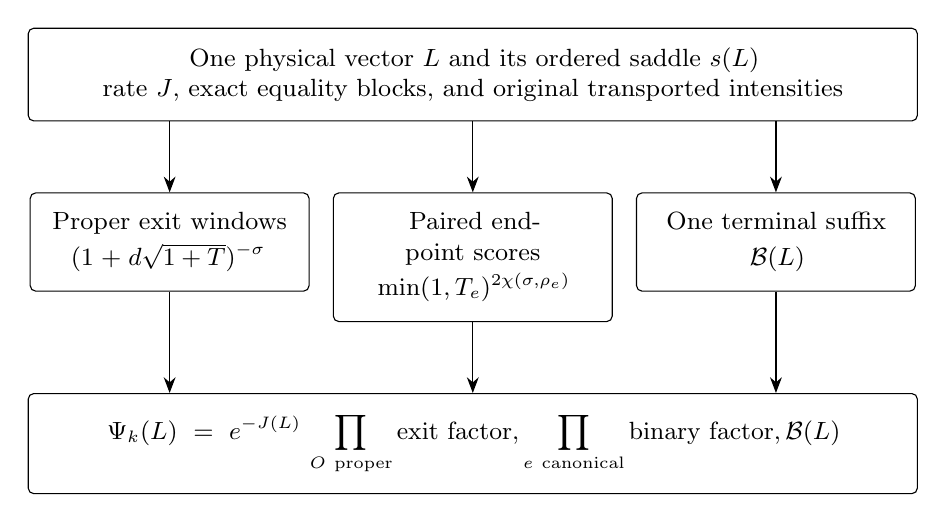
\begin{tikzpicture}[
  every node/.style={font=\small,align=center},
  box/.style={draw,rounded corners=2pt,inner sep=7pt},
  arr/.style={-{Stealth[length=2mm]},thin}]
\node[box,text width=10.8cm] (saddle)
 {One physical vector $L$ and its ordered saddle $s(L)$\\
  rate $J$, exact equality blocks, and original transported intensities};
\node[box,text width=3.05cm,below=9mm of saddle,xshift=-3.85cm] (count)
 {Proper exit windows\\[2pt]
  $(1+d\sqrt{1+T})^{-\sigma}$};
\node[box,text width=3.05cm,below=9mm of saddle] (binary)
 {Paired endpoint scores\\[2pt]
  $\min(1,T_e)^{2\chi(\sigma,\rho_e)}$};
\node[box,text width=3.05cm,below=9mm of saddle,xshift=3.85cm] (ordinary)
 {One terminal suffix\\[2pt]
  $\mathcal B(L)$};
\draw[arr] (saddle.south -| count.north) -- (count.north);
\draw[arr] (saddle.south) -- (binary.north);
\draw[arr] (saddle.south -| ordinary.north) -- (ordinary.north);
\node[box,text width=10.8cm,below=9mm of binary] (profile)
 {$\Psi_k(L)=e^{-J(L)}\,
    \displaystyle\prod_{O\text{ proper}}\text{exit factor},
    \displaystyle\prod_{e\text{ canonical}}\text{binary factor},
    \mathcal B(L)$};
\draw[arr] (count.south) -- (profile.north -| count.south);
\draw[arr] (binary.south) -- (profile.north);
\draw[arr] (ordinary.south) -- (profile.north -| ordinary.south);
\end{tikzpicture}
\caption{The deterministic construction of the positive-length profile.
The arrows indicate dependence on the same saddle data. The product
formula is established by the lower and upper proofs; it does not
assert independence of the count and path events.}
\label{fig:profile-structure}
\end{figure}


\subsection{The profile on the full parameter domain}
For $\ell_i\geq\log3$ put $L_i=\ell_i-\log3$, $A_k=2(k+1)^3$,
and define
\begin{equation}
 \Phi_k(\ell)=\inf_{\lambda\geq1}
     e^{A_k\lambda}\Psi_k\big((\max(L_i,\lambda))_{i=1}^k\big).
 \label{profile:final}
\end{equation}
This completes the numerical definition with one scalar optimization;
$\chi$ is the universal scalar specified in \eqref{profile:chi}.


Lemma~\ref{profile:finite-search} gives an explicit finite interval for
this last infimum and proves that $0<\Phi_k(\ell)<\infty$.
Every candidate length vector uses its own maximizer, exact equality
blocks, endpoint contexts and ordinary suffix.

\section{Reading the profile in concrete families}\label{sec:examples}

The exponential term alone does not distinguish all the regimes of the
answer.  The following families separate three further effects: the
comparison of named suffixes, the count associated with leaving an owner,
and the ordinary terminal constraint.  They also show how several
comparisons combine, first within one owner and then across different
owners.  Every partition into owners below is the partition of the actual
maximizer of \eqref{profile:saddle}.

Throughout this section, \(\log3+L\) means coordinatewise addition.  A
length vector specifies actual arithmetic cutoffs by
\[
 y_0=3,\qquad \log y_i=e^{L_i}\log y_{i-1}.
\]
Consequently every displayed estimate for \(\Phi_k(\log3+L)\) is also
an estimate for \(H^{(k+1)}(x,\mathbf y,2\mathbf y)/x\) throughout the
admissible region in Theorem~\ref{paper:main-H}.  Taking \(N_i=2y_i\)
for \(i\le k\) and \(N_{k+1}\ge N_k\) gives the corresponding
multiplication-table estimate by Theorem~\ref{paper:main-table}.
The dimension is fixed in all comparisons.  A constant denoted by \(C\)
is chosen once, sufficiently large in terms of that dimension.

For convenient reference, write the correlation in
\eqref{profile:edge-factor} as
\begin{equation}
 \rho(r,q;z)=
 \frac{\{\log(r+z)-p\log(q+z)\}^2}
 {\{\log(r+z)-p\log(q+z)\}^2+
             \{\log(q+z)\}^2p(1-p)},\qquad
 p=\frac{q+z}{r+z}.
 \label{ex:rho}
\end{equation}
Here \(r,q,z\) retain their meanings in the profile; in particular,
\(p\) is not the correlation.  The proofs of the evaluations, including
the finite inequalities used to locate the constants, are given in
Appendix~\ref{app:examples}.

\subsection{Equal cutoffs}

Put \(H=k+1\) and
\begin{equation}
 \alpha_H=\frac{\log((H-1)/\log H)}{\log H},\qquad
 I_H=1+(H-1)\alpha_H-H^{\alpha_H}.
 \label{ex:equal-rate}
\end{equation}
For \(L=(T,0,\ldots,0)\), the cutoffs are all \(3^{e^T}\), and
\begin{equation}
 \Phi_k(\log3+L)\asymp_k e^{-I_HT}T^{-3/2}.
 \label{ex:equal-answer}
\end{equation}
To see the factors in this formula, replace the zero lengths by a fixed
\(C\).  The resulting saddle has one terminal owner, with common product
\(\alpha_H+O_k(T^{-1})\).  All binary factors have a positive constant
lower bound.  The ordinary suffix starts in the first group, has zero
total drift, and has one group of length \(T\), followed by bounded
total length.  Its root factor is \(T^{-1/2}\) and its ballot factor is
\(T^{-1}\).  Bounded arithmetic stability transfers the estimate back
to the original equal cutoffs.  In particular the zero coordinates have
not removed any divisor coordinate.

\subsection{Three six-dimensional regimes}

The next two families have a long first group, four bounded groups, and
a long last group.  Their different relative lengths expose different
parts of the answer.

First define
\begin{gather}
 \sigma_c=1-\frac{\log((7\log7-2\log2)/5)}{\log7},\qquad
 e_h=h^{\sigma_c}\log h-(h-1),
 \label{ex:critical-constants}\\
 a=-\frac{e_7}{e_2},\qquad
 b=-\frac{e_6+e_5+e_4+e_3}{e_2},\qquad
 L=(T,C,C,C,C,aT+bC).
 \label{ex:critical-lengths}
\end{gather}
The constants satisfy \(\alpha_2<\sigma_c<\alpha_3\), \(54<a<55\),
and \(66<b<67\).  The unique saddle is exactly
\(s_1=\cdots=s_6=\sigma_c\).  Nevertheless a binary comparison remains
unsaturated.  It is the first-group edge \(6\to1\), which keeps name
\(6\) and removes names \(1,\ldots,5\).  Put
\[
 \Delta=\sum_{h=3}^6
 \left\{h^{\sigma_c-1}(h\log h-2\log2)-(h-2)\right\}>0.
\]
The pair giving the smallest endpoint scales has cuts
\[
\begin{array}{c|cc}
 &\tau_1,\ldots,\tau_5&\tau_6\\ \hline
 \text{left}&0,\ldots,0&V_6\\
 \text{right}&V_1,\ldots,V_1&V_6
\end{array}
\]
and both reference costs equal \(C\Delta\).  Both completions are late.
On the left the first group is good, and on the right it is not; the four
middle groups are good on both sides.  Thus the full scores are
\begin{equation}
 X=1+C\Delta+\sqrt T+4\sqrt C,\qquad
 Y=1+C\Delta+4\sqrt C
 \quad (T\text{ sufficiently large}).
 \label{ex:critical-endpoints}
\end{equation}
The distinction between reference cost and named endpoint score changes
the power of \(T\).  With
\(\chi_c=\chi(\sigma_c,\rho(6,1;1))\), the answer is
\begin{equation}
 \Phi_6(\log3+L)\asymp_6
       e^{-J(L)}T^{-1/2-\chi_c}.
 \label{ex:critical-answer}
\end{equation}
There is no proper-owner count.  The ordinary suffix consists of the
last group and has a drift proportional to its length, leaving only
the power \(T^{-1/2}\).  All remaining binary factors are bounded below.
The exponent is explicit: if
\(I_h^{c}=1+(h-1)\sigma_c-h^{\sigma_c}\), then
\[
 J(L)=(I_7^{c}+aI_2^{c})T+
             (I_6^{c}+I_5^{c}+I_4^{c}+I_3^{c}+bI_2^{c})C.
\]

Now move the last cutoff much farther away by taking
\begin{equation}
 L=(T,0,0,0,0,T^3).
 \label{ex:split-lengths}
\end{equation}
Write \(\alpha=\alpha_2\).  There is a unique \(s_*\in(\alpha,1)\)
satisfying
\begin{equation}
 z_*=2^{\alpha/s_*},\qquad
 (5+z_*)^{s_*-1}
 \{(5+z_*)\log(5+z_*)-z_*\log z_*\}=5;
 \qquad 0.54070<s_*<0.54072.
 \label{ex:split-root}
\end{equation}
After replacing the four zero lengths by \(C\), the actual owners are
\([1,5]\) and \([6]\).  Their products tend to \(s_*\) and \(\alpha\),
respectively.  Only the proper edge \(5\to0\) in the first group is
unsaturated.  Its endpoint scales are both bounded, giving
\(T^{-2\chi_*}\), where
\(\chi_*=\chi(s_*,\rho(5,0;z_*))\).  The proper count gives
\(T^{-s_*/2}\).  The terminal length is \(T^3\), but its drift has order
\(T\), supplied by the earlier owner.  Hence its joint ordinary and root
factor is \(T(T^3)^{-3/2}\).  Altogether, with
\[
 I_2=1+\alpha-2^\alpha,\qquad
 I_{\rm p}=1+5s_*+\alpha-(5+z_*)^{s_*},
\]
we obtain
\begin{equation}
 \Phi_6(\log3+L)\asymp_6
 e^{-I_2T^3-I_{\rm p}T}
 T^{1-s_*/2-2\chi_*}(T^3)^{-3/2}.
 \label{ex:split-answer}
\end{equation}
The child in this proper comparison has \(z_*>1\), so \(q=0\) still
leaves a nondegenerate binary mark.  It is distinct from the terminal
ordinary comparison.

There is a precise dimensional reason for using six coordinates in
these two families.  For the first construction, replacing \(7\) by
\(H\) in \eqref{ex:critical-constants} gives a product below
\(\alpha_2\) for \(3\le H\le6\), and above it for \(H=7\).  For the
second, the boundary sign is
\[
 f(H)=H^{\alpha-1}(H\log H-2\log2)-(H-2),\qquad
 f(6)>0>f(7).
\]
Strict concavity of \(f\) on \([2,\infty)\) makes the strict branch
possible precisely for \(H\ge7\) in this two-scale family.  These are
thresholds for the stated constructions, not classifications of all
parameter vectors.

A final contrast isolates the proper count.  Fix
\(s=107/200\), \(\theta=267/500\), and \(z=2^{\theta/s}\).  Set
\begin{gather}
 f_r=(r+z)^{s-1}E_r(z)-r,\qquad
 c_r=1-z\log2\,(r+z)^{s-1},\nonumber\\
 a=-\frac{f_1+f_2+f_3+f_4}{f_5},\qquad
 b=\frac{ac_5+c_1+c_2+c_3+c_4}{2^\theta\log2-1},\qquad
 L=t(a,1,1,1,1,b).
 \label{ex:ray-lengths}
\end{gather}
Here \(a\) and \(b\) are positive (approximately \(10.958044\) and
\(1651.936051\)).  The exact owners remain \([1,5]\), \([6]\), with
products \(s,\theta\), but every binary factor is bounded below.
Writing \(J_0=J(a,1,1,1,1,b)\), we have
\begin{equation}
 \Phi_6(\log3+L)\asymp_6 e^{-tJ_0}t^{-(1+s)/2}.
 \label{ex:ray-answer}
\end{equation}
Thus leaving an owner can impose a count penalty even when every binary
comparison has sufficient endpoint room.

\subsection{Two comparisons in one owner}

The next family has two unsaturated edges in the same proper owner.
They share its count factor, but have different endpoint scales and
different correlations.

For \(x>y\ge1\), define
\[
 t(x,y)=1-\frac{\log((x\log x-y\log y)/(x-y))}{\log x}.
\]
Let \(z\) be the unique solution in \((1.98455,1.98457)\) of
\begin{equation}
 t(14+z,6+z)=t(6+z,z),\qquad
 \sigma=t(6+z,z),\qquad \theta=\frac{\sigma\log z}{\log2}.
 \label{ex:same-root}
\end{equation}
Then \(\alpha_2<\theta<\sigma\), with
\(\sigma\) approximately \(0.551693\) and \(\theta\) approximately
\(0.545525\).  For \(1\le r\le14\), put
\[
 \kappa_r=(r+z)^{\sigma-1},\qquad
 f_r(q)=q-\kappa_r E_q(z),\qquad g_r=f_r(r).
\]
The defining equations give the exact identities
\begin{equation}
 g_6=0,\qquad f_{14}(6)=g_{14}>0,
 \qquad g_1<0.
 \label{ex:same-balances}
\end{equation}
Take \(k=15\), \(U=T^3\), and specify the lengths by
\begin{align}
 &L_1=T,\quad L_9=U,\quad
 L_i=C\quad(2\le i\le13,\ i\ne9),\nonumber\\
 &L_{14}=W=-\frac{g_{14}T+
                C\sum_{\substack{2\le r\le13\\r\ne6}}g_r}{g_1},
 \qquad
 L_{15}=R=
 \frac{\sum_{i=1}^{14}L_i(1-z\log2\,\kappa_{15-i})}
 {2^\theta\log2-1}.
 \label{ex:same-lengths}
\end{align}
All these lengths are positive; \(W\asymp T\) and \(R\asymp U\).
The actual saddle is
\((\sigma,\ldots,\sigma,\theta)\), so the owners are \([1,14]\) and
\([15]\).  The two equations defining \(W,R\) balance the common
proper-owner direction and the terminal direction.  The remaining KKT
inequalities are strict.

The first rare comparison is \(14\to6\) in group \(1\).  Keeping the
six deepest names until their deadlines gives equal bounded reference
costs at its endpoints.  The left completion makes the first group good,
while the right completion does not.  The second rare comparison is
\(6\to0\) in group \(9\).  Its six names must survive through the
earlier first group, and this creates a cost of order \(T\) at both
endpoints.  Precisely,
\begin{equation}
 (X_{1,6},Y_{1,6})\asymp(\sqrt T,1),\qquad
 (X_{9,0},Y_{9,0})\asymp(T,T).
 \label{ex:same-endpoints}
\end{equation}
Every other binary factor is bounded below.  Put
\[
 \chi_1=\chi(\sigma,\rho(14,6;z)),\qquad
 \chi_2=\chi(\sigma,\rho(6,0;z)).
\]
There is one proper count, of order \(U^{-\sigma/2}\), and one ordinary
root factor, of order \(U^{-1/2}\).  The resulting full profile is
\begin{equation}
 \Phi_{15}(\log3+L)\asymp_{15}
 e^{-J(L)}U^{-(1+\sigma)/2}T^{-\chi_1}
                   \left(\frac{T^2}{U}\right)^{2\chi_2},
 \qquad U=T^3.
 \label{ex:same-answer}
\end{equation}
Its exponential is explicit as well:
\begin{equation}
 J(L)=\sum_{i=1}^{14}L_i
  \{1+(15-i)\sigma+\theta-(15-i+z)^\sigma\}
       +R(1+\theta-2^\theta).
 \label{ex:same-rate}
\end{equation}
This example explains why the profile takes the product of all canonical
edge factors inside an owner, but assigns a count factor only once to
that owner.  No assertion of independence between the two comparisons
is involved.

\subsection{Two comparisons in different owners}

One more family makes the different owner powers visible.  Put
\(k=18\), \(\alpha=\alpha_2\), and, for \(c>0\), define
\[
 F(s;c)=(1+e^{c/s})^{s-1}
       \{(1+e^{c/s})\log(1+e^{c/s})-e^{c/s}(c/s)\}-1.
\]
Let \(v,u\) be the roots
\begin{equation}
 F(v;\alpha\log17)=0,\qquad
 G_2^*=v\log(1+17^{\alpha/v}),\qquad F(u;G_2^*)=0.
 \label{ex:multi-roots}
\end{equation}
They are uniquely determined in \((0,1)\) and satisfy
\(u>v>\alpha\); approximately they are
\(u=0.534353736\), \(v=0.531542356\).
Set
\begin{gather}
 z_2^*=17^{\alpha/v},\quad z_1^*=e^{G_2^*/u},\quad
 Z_j^*=(1+z_j^*)^{s_j^*},\quad (s_1^*,s_2^*)=(u,v),\nonumber\\
 L_1=T,\quad L_2=T^3,\quad
 L_i=2^{i-3}T^5\ (3\le i\le17),\quad L_{18}=T^{11}.
 \label{ex:multi-lengths}
\end{gather}
For sufficiently large \(T\), the exact owners are
\([1]\), \([2]\), \([3,18]\).  Their products satisfy
\[
 u_T=u+O(T^{-2}),\qquad v_T=v+O(T^{-2}),\qquad
 \tau_T=\alpha+O(T^{-6}).
\]
Each of the first two owners has just the proper edge \(1\to0\).
Their endpoint scales are
\[
 (X_1,Y_1)\asymp(1,1),\qquad
 (X_2,Y_2)\asymp(T,1).
\]
The old first group supplies the left endpoint room in the second
comparison.  With
\(\chi_1=\chi(u,\rho(1,0;z_1^*))\) and
\(\chi_2=\chi(v,\rho(1,0;z_2^*))\), the respective binary costs are
\(T^{-2\chi_1}\), \(T^{-4\chi_2}\), and the respective count costs
are \(T^{-u/2}\), \(T^{-3v/2}\).

All \(120\) terminal binary factors have a positive constant lower
bound.  The ordinary suffix is the last group: its length is \(T^{11}\)
and its drift has order \(T^5\).  Its single joint factor is therefore
\(T^{-23/2}\).  Define
\begin{align}
 J_0(T)={}&T(1+u+v+16\alpha-Z_1^*)
       +T^3(1+v+16\alpha-Z_2^*)\nonumber\\
 &+T^5\sum_{i=3}^{17}2^{i-3}
       \{1+(h_i-1)\alpha-h_i^\alpha\}
       +T^{11}(1+\alpha-2^\alpha),\qquad h_i=20-i.
 \label{ex:multi-rate}
\end{align}
Then \(J(L)=J_0(T)+O(T^{-1})\), and
\begin{equation}
 \Phi_{18}(\log3+L)\asymp_{18}
 e^{-J_0(T)}
 T^{-23/2-u/2-3v/2-2\chi_1-4\chi_2}.
 \label{ex:multi-answer}
\end{equation}
Thus the two owners contribute their own powers and counts, while the
whole chain still has only one ordinary root.

For this particular construction the dimensional threshold is governed
by a one-step, rather than a long-interval, secant.  If
\[
 t_1(x)=1-\frac{\log\{x\log x-(x-1)\log(x-1)\}}{\log x},
\]
then \(t_1(17)<\alpha_2<t_1(18)\).  Together with the one-valley
property in Lemma~\ref{hier:lem:valley}, this says that a terminal child
with limiting product \(\alpha_2\) needs at least \(17\) names before
the adjacent singleton can have a strictly larger product.  Two such
singleton owners therefore first fit in dimension \(18\).  This
statement concerns the specified singleton construction; the
fifteen-dimensional example uses a different arrangement of ranks.

\section{Geometry of the ordered saddle}\label{sec:geometry}\label{paper:geometry}

The optimizer does more than select the exponential scale of the answer.
Its equality blocks determine which count windows are narrow, and its
first derivatives give the budgets available to the path constraints.
We begin with a general finite rank chain, since restrictions to equality
subspaces arise naturally when parameters move. We then specialize to the
complete chain needed for the divisor problem.

\subsection{The objective and the main conclusions}

Fix integers
\[
 H=h_1>h_2>\cdots>h_m\ge 2,
\]
where the one-element chain is allowed.  Set
\[
 p_i=h_i-h_{i+1}\quad(i<m),\qquad p_m=h_m-1,
 \qquad V_j=\sum_{i=1}^j L_i,\quad V_0=0,
\]
with arbitrary \(L_i>0\).  The symbols \(p_i\) always denote these
positive integers.  Child probabilities will instead be denoted by
\(\beta_i\).

On the ordered simplex
\[
 \calD=\{s\in\R^m:1\ge s_1\ge\cdots\ge s_m\ge0\}
\]
define, first at positive products,
\begin{align}
 G_m(s)&=s_m\log h_m,\nonumber\\
 G_i(s)&=s_i\log\bigl(p_i+\exp(G_{i+1}(s)/s_i)\bigr)
                   &&(i<m),\label{geom:eq:recursion}\\
 Z_i(s)&=\exp G_i(s),\nonumber\\
 J(L;s)&=\sum_iL_i+\sum_j s_jp_jV_j-\sum_iL_iZ_i(s).
                                                        \label{geom:eq:objective}
\end{align}
Use the continuous extension at zero products.  Indeed, induction gives
\(0\le G_i(s)\le s_i\log h_i\): if
\(G_{i+1}\le s_{i+1}\log h_{i+1}\), ordering gives
\(\exp(G_{i+1}/s_i)\le h_{i+1}\).  Thus when \(s_i=0\) its whole
suffix is zero and \(G_i=0\), \(Z_i=1\).  In particular,
\begin{equation}
 1\le Z_i(s)\le h_i \qquad(s\in\calD).             \label{geom:eq:globalZ}
\end{equation}

For \(E\subseteq\{1,\ldots,m-1\}\), let
\[
 \calD_E=\{s\in\calD:s_j=s_{j+1}\text{ for every }j\in E\}.
\]
Every maximum below is over this \emph{whole} feasible set.  Equalities
not specified by \(E\), and all other order inequalities, remain part
of the optimization.  Write \(s^E(L)\) for the maximizer and
\(J_E^*(L)=J(L;s^E(L))\).  Existence and uniqueness will be proved.

Throughout, \(c,C>0\) may change from line to line and depend only on
the fixed chain.  In particular they do not depend on \(L\), its ratios,
the face \(E\), or the sizes of product gaps and multipliers.  The notation
\(A\asymp B\) means \(cB\le A\le CB\), with this convention.

\begin{theorem}[Global bounds]\label{geom:thm:global}
Put
\begin{equation}
 c_0=2\log2-1,\qquad
 \varepsilon_H=\frac{c_0}{2H(\log H)^2}.             \label{geom:eq:epsilon}
\end{equation}
For every positive length vector and every \(E\), there is a unique
maximizer on \(\calD_E\), and it satisfies
\begin{equation}
 \frac12<s_m^E(L)\le s_1^E(L)<1-\varepsilon_H.
                                                        \label{geom:eq:outer}
\end{equation}
\end{theorem}

At a face maximizer define the signed cumulative multipliers
\begin{equation}
 \lambda_j^E(L)=-\sum_{i\le j}\partial_{s_i}J(L;s^E(L)),
 \qquad \lambda_0^E=\lambda_m^E=0.                 \label{geom:eq:lambda}
\end{equation}
The equality for \(\lambda_m^E\) follows from stationarity in the common
product direction.  For \(j\notin E\), these multipliers are nonnegative
and complementary to \(s_j^E-s_{j+1}^E\).  For \(j\in E\) they are signed.

\begin{theorem}[Stability across changing active faces]\label{geom:thm:stability}
Fix \(E\), let \(L'=L+\Delta\), and assume
\(|\Delta_i|\le L_i/2\).  Put \(D=\sum_i|\Delta_i|\).  Then
\begin{align}
 |s_i^E(L')-s_i^E(L)|
   &\le C\sum_{\ell=1}^m
                \frac{|\Delta_\ell|}{V_{\max(i,\ell)}},   \label{geom:eq:stability}\\
 |J_E^*(L')-J_E^*(L)|&\le CD,                           \label{geom:eq:value}\\
 |\lambda_j^E(L')-\lambda_j^E(L)|&\le CD.                \label{geom:eq:multiplier}
\end{align}
No extra lower threshold for the lengths is required.  The active
inequalities outside \(E\) may appear, disappear, or remain degenerate
along the perturbation.
\end{theorem}

For \(x\in\calD\), write \(\gap_j(x)=x_j-x_{j+1}\).
Let \(\bar s=s^E(L)\), \(s^*=s^\varnothing(L)\), and set
\begin{equation}
 a_j=
 \begin{cases}(-\lambda_j^E(L))_+,&j\in E,\\0,&j\notin E,\end{cases}
 \qquad \mathcal A_E=\sum_{j<m}\frac{a_j^2}{V_j}.       \label{geom:eq:AE}
\end{equation}

\begin{theorem}[Release of equalities]\label{geom:thm:opening}
Uniformly in \(L\) and \(E\),
\begin{align}
 J_\varnothing^*(L)-J_E^*(L)&\asymp\mathcal A_E,       \label{geom:eq:openingrate}\\
 \sum_i V_i(s_i^*-\bar s_i)^2&\asymp\mathcal A_E.     \label{geom:eq:openingdisp}
\end{align}
Both quantities are zero when \(\mathcal A_E=0\).
For \(E=\{j\}\), put \(a=(-\lambda_j^E)_+\).  If \(a=0\),
then \(\bar s=s^*\).  If \(a>0\), additionally
\begin{equation}
 \gap_j(s^*)\asymp \frac a{V_j},\qquad
 J_\varnothing^*(L)-J_{\{j\}}^*(L)\asymp\frac{a^2}{V_j}.
                                                        \label{geom:eq:single}
\end{equation}
The individual-gap assertion is only made for a single released edge.
\end{theorem}

We prove these estimates directly from the finite objective. The curvature
controls each suffix on its own cumulative length scale; this is the
reason that perturbations remain controlled when the active equality
constraints change.

\subsection{Concavity and the outer boundaries}

The map \(x\mapsto\log(p+e^x)\) is convex and increasing.  Its
perspective \((s,y)\mapsto s\log(p+e^{y/s})\) is convex for \(s>0\)
and is increasing in \(y\).  Induction in \eqref{geom:eq:recursion} therefore
shows that each \(G_i\), and hence each \(Z_i\), is convex.  The continuous
extension gives convexity on \(\calD\).  Thus \(J\) is concave and
continuous on the compact convex set \(\calD_E\), so a maximum exists.

\subsubsection{The bottom plateau}

\begin{lemma}\label{geom:lem:bottom}
Every maximizer on \(\calD_E\) satisfies \(s_m>1/2\).
\end{lemma}

\begin{proof}
Suppose that \(a,\ldots,m\) is the maximal bottom block of equal
products, with common value \(\sigma\le1/2\).  Increasing this entire
block by a small positive amount is feasible.  If \(a>1\), its preceding
gap is strict, so no prescribed equality crosses that gap.  Exact
telescoping gives
\[
 G_i=\sigma\log h_i,\qquad Z_i=h_i^\sigma\quad(i\ge a).
\]
For \(i<a\), set
\[
 \beta_i=\frac{\exp(G_{i+1}/s_i)}
                    {p_i+\exp(G_{i+1}/s_i)}.
\]
Along this bottom-block direction,
\[
 \frac{dG_i}{d\sigma}
   =\left(\prod_{i\le b<a}\beta_b\right)\log h_a.
\]
The identity
\[
 Z_i\beta_i=Z_{i+1}\beta_i^{\,1-s_i}
\]
implies
\[
 Z_i\prod_{i\le b<a}\beta_b
   = Z_a\prod_{i\le b<a}\beta_b^{\,1-s_b}\le Z_a.
\]
When \(\sigma=0\), all preceding products, if present, are positive,
and these formulas give the right derivative.  There are no preceding
terms if \(a=1\).

The derivative of the linear budget is
\[
 \sum_{j\ge a}p_jV_j
   =(h_a-1)V_{a-1}+\sum_{i\ge a}(h_i-1)L_i.
\]
Consequently the directional derivative of \(J\) is at least
\begin{equation}
 V_{a-1}(h_a-1-h_a^\sigma\log h_a)
       +\sum_{i\ge a}L_i(h_i-1-h_i^\sigma\log h_i). \label{geom:eq:bottomderivative}
\end{equation}
For every real \(h>1\), one has \(\sqrt h\log h<h-1\).
Indeed, with \(t=\sqrt h\), the difference
\(t^2-1-2t\log t\) vanishes at \(1\) and has positive derivative
\(2(t-1-\log t)\) for \(t>1\).
Every bracket in \eqref{geom:eq:bottomderivative} is thus positive.
Since the lengths are positive, the derivative is strictly positive.
This contradicts maximality, including at \(\sigma=0\).
\end{proof}

\subsubsection{The top plateau}

\begin{lemma}\label{geom:lem:top}
Every maximizer on \(\calD_E\) satisfies \(s_1<1-\varepsilon_H\).
\end{lemma}

\begin{proof}
Let \(1,\ldots,b\) be the maximal top equal-product block, with
common value \(\sigma\).  If \(b<m\), put
\(C=h_{b+1}\) and \(z=\exp(G_{b+1}/\sigma)\); otherwise put \(C=z=1\).
For \(i\le b\), let \(n_i=h_i-C\ge1\).  Telescoping yields
\[
 G_i=\sigma\log(n_i+z).
\]
Here \(1\le z\le C\) and \(n_i+z\le H\), by the ordered recursion.
Varying the top block while keeping its child products fixed gives
\begin{equation}
 \frac{dZ_i}{d\sigma}=(n_i+z)^\sigma A(n_i,z),\qquad
 A(n,z)=\log(n+z)-\frac{z\log z}{n+z}.             \label{geom:eq:topderivative}
\end{equation}
This formula includes the variation of \(z=\exp(G_{b+1}/\sigma)\).
The budget derivative is \(\sum_{i\le b}L_i n_i\).

Write
\[
 E_n(z)=(n+z)\log(n+z)-z\log z=(n+z)A(n,z).
\]
It is increasing in \(z\), since \(\partial_zE_n=\log(1+n/z)>0\).
Moreover
\[
 E_n(z)\ge E_n(1)=(n+1)\log(n+1)\ge2n\log2.
\]
For the last inequality,
\((n+1)\log(n+1)/n\) is increasing for \(n>0\), with derivative
\([n-\log(n+1)]/n^2>0\), and \(n\ge1\).
Also \(0<A(n,z)\le\log H\).  With \(n,z\) fixed at their values
at the point under consideration, for \(0\le\tau\le1\),
\[
 \frac{d}{d\tau}\bigl((n+z)^\tau A(n,z)\bigr)
 \le H(\log H)^2.
\]
This auxiliary comparison keeps \(z\) fixed.
If \(\sigma\ge1-\varepsilon_H\), it follows that
\[
 (n+z)^\sigma A(n,z)-n
 \ge n(2\log2-1)-\varepsilon_HH(\log H)^2
 \ge c_0/2>0.
\]
Thus raising the top block has strictly negative derivative for \(J\).
Lowering it a sufficiently small amount is feasible and increases
\(J\), a contradiction.  This also covers \(\sigma=1\).
\end{proof}

Let \(\varepsilon=\varepsilon_H\), which lies in \((0,1/2)\), and put
\[
 \calD_\varepsilon
   =\{s:\varepsilon\le s_m\le\cdots\le s_1\le1-\varepsilon\}.
\]
The preceding lemmas put every maximizer on every prescribed face in
this single compact set.  We will use differential estimates on the
slightly larger convex set \(\calD_{\varepsilon/2}\).

\subsection{Full suffix curvature and uniqueness}

For \(i<m\), introduce
\[
 a_i=G_i/s_i=\log S_i,\qquad
 u_i=s_{i+1}/s_i,\qquad
 \beta_i=\frac{e^{G_{i+1}/s_i}}{S_i},\qquad
 A_i=a_i-u_i\beta_i a_{i+1},
\]
where \(S_i=p_i+e^{G_{i+1}/s_i}\); set
\(a_m=A_m=\log h_m\).
All these functions and the derivatives needed below are bounded on
\(\calD_{\varepsilon/2}\).  The quantities \(s_i,a_i,\beta_i,1-\beta_i\)
have positive chain-dependent lower bounds.  The same holds for \(A_i\):
it is the entropy of the distribution consisting of \(p_i\) named
probabilities \(1/S_i\) and the one compound probability \(\beta_i\).
These assertions use compactness but no separation of adjacent products.

\begin{lemma}[One perspective term controls its entire suffix]
\label{geom:lem:suffix}
For any \(s\in\calD_{\varepsilon/2}\), direction \(z\in\R^m\), and \(i\),
\begin{equation}
 c\sum_{j\ge i}z_j^2\le D^2Z_i(s)[z,z]
                   \le C\sum_{j\ge i}z_j^2.      \label{geom:eq:suffix}
\end{equation}
\end{lemma}

\begin{proof}
Let \(g_i=DG_i[z]\) and \(Q_i=D^2G_i[z,z]\).  Differentiating the
perspective recursion gives
\begin{align}
 g_m&=(\log h_m)z_m,\qquad Q_m=0,\nonumber\\
 g_i&=A_i z_i+\beta_i g_{i+1},\nonumber\\
 Q_i&=\beta_iQ_{i+1}
  +\frac{\beta_i(1-\beta_i)}{s_i}
              (g_{i+1}-u_i a_{i+1}z_i)^2.        \label{geom:eq:perspectivecurvature}
\end{align}
In particular \(Q_i\ge0\).  Put \(E_i=g_i^2+Q_i\) and
\(w_i=g_{i+1}-u_i a_{i+1}z_i\).  Then
\[
 g_i=a_i z_i+\beta_iw_i,\qquad
 Q_i\ge c w_i^2+cQ_{i+1}.
\]
Thus \(z_i^2\le CE_i\), and then \(g_{i+1}^2\le CE_i\), so that
\(E_{i+1}\le CE_i\).  Iteration over the fixed number of indices,
starting with \(E_m=(\log h_m)^2z_m^2\), proves
\[
 E_i\ge c\sum_{j\ge i}z_j^2.
\]
The reverse inequality follows recursively from
\eqref{geom:eq:perspectivecurvature} and its bounded coefficients.
Finally,
\[
 D^2Z_i[z,z]=Z_iE_i,
\]
and \(Z_i\) is bounded above and below.
\end{proof}

Define the negative objective Hessian by
\(\calH(L;s)=-D_s^2J(L;s)\).
Summing \eqref{geom:eq:suffix} with weights \(L_i\) gives
\begin{equation}
 c\sum_jV_j z_j^2
 \le z^{\mathsf T}\calH(L;s)z
 \le C\sum_jV_j z_j^2.                            \label{geom:eq:hessian}
\end{equation}
Furthermore,
\begin{equation}
 |\calH_{ij}(L;s)|\le C V_{\min(i,j)},             \label{geom:eq:hessianentry}
\end{equation}
because only terms \(L_\ell Z_\ell\) with \(\ell\le\min(i,j)\)
depend on both coordinates, and their second derivatives are bounded.
These estimates hold for every positive length vector, without
stationarity or a length hierarchy.

If two distinct maximizers existed on \(\calD_E\), concavity would
make their whole connecting segment maximizing.  The global boundary
lemmas put that segment in \(\calD_\varepsilon\), whereas
\eqref{geom:eq:hessian} makes the restriction to the segment strictly concave.
This contradiction proves uniqueness and finishes
Theorem~\ref{geom:thm:global}.

\subsection{An LDL inverse estimate on every equality subspace}

\begin{lemma}\label{geom:lem:inverse}
Suppose that a symmetric positive definite \(r\times r\) matrix \(A\)
and increasing positive numbers \(W_1,\ldots,W_r\) satisfy
\[
 c\diag(W)\le A\le C\diag(W),\qquad
 |A_{ij}|\le C W_{\min(i,j)}.
\]
Then
\begin{equation}
 |(A^{-1})_{ij}|\le\frac{C'}{W_{\max(i,j)}},       \label{geom:eq:inverse}
\end{equation}
where \(C'\) depends only on \(r,c,C\).
\end{lemma}

\begin{proof}
Perform scalar LDL elimination in the order \(1,\ldots,r\).
Every Schur complement retains the same diagonal quadratic bounds:
its quadratic form is obtained by minimizing the preceding form over
the eliminated coordinates.  The lower bound follows by discarding
the nonnegative eliminated diagonal terms; for the upper bound choose
those coordinates to be zero.  Thus the pivot at index \(i\) is
comparable to \(W_i\).

The entry estimate also persists, with constants depending on the
number of steps.  When index \(i\) is eliminated, the update in entry
\(j,\ell>i\) is bounded by
\[
 C\,\frac{W_iW_i}{W_i}=CW_i
       \le CW_{\min(j,\ell)}.
\]
Every multiplier in the unit lower triangular elimination matrix is
therefore bounded.  Its inverse has bounded entries as well, by the
finite nilpotent series for the strictly lower triangular part.
If \(A=\mathsf L\,\mathsf D\,\mathsf L^{\mathsf T}\), the \(i,j\) entry
of \(A^{-1}=\mathsf L^{-\mathsf T}\mathsf D^{-1}\mathsf L^{-1}\)
is a sum over indices \(t\ge\max(i,j)\) of bounded numerators divided
by pivots comparable to \(W_t\).  Monotonicity of \(W_t\) proves
\eqref{geom:eq:inverse}.
\end{proof}

Partition \(\{1,\ldots,m\}\) into consecutive blocks \(I_a=[b_a,e_a]\).
Let \(B\) map block coordinates to vectors constant on each block.
The restricted Hessian is \(A=B^{\mathsf T}\calH B\).
By \eqref{geom:eq:hessian}, its natural quadratic weights are
\(\sum_{j\in I_a}V_j\), which lie between \(V_{e_a}\) and \(mV_{e_a}\).
For \(a<b\), summing \eqref{geom:eq:hessianentry} over the two blocks gives
\(|A_{ab}|\le C V_{e_a}\).  Lemma~\ref{geom:lem:inverse} consequently gives
\begin{equation}
 \left|\bigl((B^{\mathsf T}\calH B)^{-1}\bigr)_{ab}\right|
       \le \frac C{V_{\max(e_a,e_b)}}.            \label{geom:eq:restrictedinverse}
\end{equation}
There are only finitely many such partitions, so a single constant
works for all of them.  The Hessian is that of the original objective
restricted to its current equality subspace.

\subsection{Moving optimizers and differentiation across faces}

We first record the elementary KKT relations with the sign convention
in \eqref{geom:eq:lambda}.  At a maximizer on \(\calD_E\), a small shift of
all products in either direction is feasible by
Theorem~\ref{geom:thm:global}; hence \(\sum_i\partial_iJ=0\).
For \(j\notin E\), increasing the first \(j\) coordinates is feasible
even when \(\gap_j=0\).  Its derivative is \(-\lambda_j\), so
\(\lambda_j\ge0\).  If \(\gap_j>0\), shifting that prefix in either
direction is feasible, giving \(\lambda_j=0\).  Thus
\begin{equation}
 \partial_iJ=\lambda_{i-1}-\lambda_i,\qquad
 \lambda_j\ge0,\quad\lambda_j\gap_j=0\quad(j\notin E).
                                                        \label{geom:eq:KKT}
\end{equation}
The multipliers at edges in \(E\) are not sign constrained.
Conversely, \eqref{geom:eq:KKT}, the signed equalities, and concavity
give the corresponding global variational inequality.

Fix \(E\), and consider \(L(t)=L+t\Delta\), \(0\le t\le1\), with
\(|\Delta_i|\le L_i/2\).  Then
\begin{equation}
 \tfrac12 V_j\le V_j(t)\le\tfrac32 V_j.            \label{geom:eq:Vcompare}
\end{equation}
Let \(s(t)=s^E(L(t))\).  All of these true constrained maxima lie in
\(\calD_\varepsilon\), by the global theorem.

\begin{lemma}\label{geom:lem:AC}
The path \(s(t)\), and all gradient components along it, are Lipschitz
and hence absolutely continuous.  At almost every \(t\), its derivative
is constant on each maximal block of equal current products.
\end{lemma}

\begin{proof}
Continuity follows from compactness and uniqueness: any convergent
subsequence of maximizing points as \(t_n\to t\) maximizes the limiting
objective, so its limit is \(s(t)\).

For \(t,t'\), the two constrained variational inequalities and strong
concavity on the segment joining the maximizers give, with
\(d=s(t')-s(t)\),
\[
 cV_1\|d\|^2
 \le \left|\bigl(\nabla J(L(t');s(t'))
                 -\nabla J(L(t);s(t'))\bigr)\cdot d\right|
 \le C|t'-t|D\|d\|.
\]
Here the first bound uses \eqref{geom:eq:hessian} and
\eqref{geom:eq:Vcompare}, and the second uses bounded length derivatives
of the gradient.  This Lipschitz bound establishes the regularity
needed for the componentwise estimate below.
The gradient path is also Lipschitz since the objective is smooth
on the compact product set and the length path is affine.

A nonnegative absolutely continuous function has derivative zero
at almost every point of its zero set.  To see this, at a density
point of the zero set where its derivative exists, take difference
quotients along that set.  The density theorem and almost-everywhere
differentiability remove the remaining null sets.
Apply this observation to each gap \(s_i(t)-s_{i+1}(t)\).
There are finitely many gaps, so at almost every common differentiability
point, \(\dot s(t)\) is constant on every current equal-product block.
\end{proof}

At such a time, let \(I_a=[b_a,e_a]\) be the current maximal blocks,
and write \(\dot s=B\dot q\).  Both exterior gaps of a block, when
present, are strictly positive.  They stay positive in a neighborhood
of this time, and their multipliers vanish throughout that neighborhood.
No prescribed equality crosses one of these strict gaps.  Consequently,
keeping these block endpoints fixed, one has in the whole neighborhood
\begin{equation}
 \sum_{i\in I_a}\partial_iJ(L(t);s(t))=0.          \label{geom:eq:blockstationarity}
\end{equation}
This identity remains true if internal equalities split nearby.
It may therefore be differentiated at the chosen almost-everywhere
point.  This is the step that avoids assuming a differentiable
active-set chart.

Since \(J\) is linear in \(L\), define
\begin{equation}
 U_\ell(s)=\partial_{L_\ell}J
    =1+\sum_{j\ge\ell}s_jp_j-Z_\ell(s),\qquad
 b=\sum_\ell\Delta_\ell\nabla U_\ell(s(t)).
                                                        \label{geom:eq:U}
\end{equation}
Differentiating \eqref{geom:eq:blockstationarity} gives
\begin{equation}
 (B^{\mathsf T}\calH B)\dot q=B^{\mathsf T}b.     \label{geom:eq:blockODE}
\end{equation}
The vector \(\nabla U_\ell\) has zero entries before \(\ell\) and
uniformly bounded entries thereafter.  Its sum over a block can
therefore be nonzero only when that block's right endpoint is at
least \(\ell\).  By \eqref{geom:eq:restrictedinverse}, for \(i\in I_a\),
\begin{align}
 |\dot s_i(t)|
 &\le C\sum_\ell|\Delta_\ell|
      \sum_{\substack{b:\ e_b\ge\ell}}
                   \frac1{V_{\max(e_a,e_b)}(t)}\nonumber\\
 &\le C\sum_\ell\frac{|\Delta_\ell|}
                         {V_{\max(i,\ell)}(t)}.  \label{geom:eq:derivstability}
\end{align}
Indeed \(e_a\ge i\), \(e_b\ge\ell\), and there are at most \(m\)
blocks.  Integrating this almost-everywhere estimate and using
\eqref{geom:eq:Vcompare} proves \eqref{geom:eq:stability}.

\begin{remark}
An equality with zero multiplier may persist on a set of positive
measure, split, or reform.  The preceding argument includes all such
possibilities: tangency comes from absolute continuity of the gaps,
and the differentiated stationarity equation uses only the current
block's strictly separated exterior boundaries.
\end{remark}

\subsection{Values, multipliers, and own-scale parameters}

The coefficients \(U_\ell\) in \eqref{geom:eq:U} are bounded on the entire
original simplex, using \eqref{geom:eq:globalZ}.  Hence
\[
 |J(L';s)-J(L;s)|\le CD\qquad(s\in\calD).
\]
Taking the maximum on the same \(\calD_E\) in both directions proves
\eqref{geom:eq:value}.  In fact this value bound does not require the
relative perturbation assumption.

For the signed multiplier, absolute continuity and
\eqref{geom:eq:U} give almost everywhere
\[
 \dot\lambda_j
   =-\sum_{i\le j}b_i
       +\sum_{i\le j}\sum_a\calH_{ia}\dot s_a.
\]
The first term is \(O(D)\).  By \eqref{geom:eq:hessianentry} and
\eqref{geom:eq:derivstability}, the second term is at most
\[
 C\sum_{i\le j}\sum_\ell|\Delta_\ell|
          \sum_a\frac{V_{\min(i,a)}(t)}
                       {V_{\max(a,\ell)}(t)}.
\]
Every fraction is at most one.  The finite sums are therefore
\(O(D)\), uniformly in all length ratios.  Integration proves
\eqref{geom:eq:multiplier} and finishes Theorem~\ref{geom:thm:stability}.
In particular the bound applies to the unrestricted signed
multipliers at prescribed equality edges.

\begin{corollary}[Own-scale exponent stability]\label{geom:cor:ownscale}
Let \(F_i(s_i,\ldots,s_m)\) be bounded and Lipschitz on
\(\calD_{\varepsilon/2}\), with chain-dependent bounds.  Under the
hypotheses of Theorem~\ref{geom:thm:stability},
\begin{equation}
 |F_i(s^E(L'))-F_i(s^E(L))|\le \frac{CD}{V_i}.
                                                        \label{geom:eq:ownscale}
\end{equation}
For \(D\) bounded, each of the factors
\[
 (1+L_i)^{F_i(s^E(L))},\qquad
 \left(\frac{1+V_{i-1}}{1+L_i}\right)^{F_i(s^E(L))}
\]
changes by a bounded multiplicative factor when \(L\) is replaced
by \(L'\).  The bound does not involve a logarithm of a more remote
length.
\end{corollary}

\begin{proof}
For every suffix coordinate \(j\ge i\), \eqref{geom:eq:stability} is
bounded above by \(CD/V_i\), proving \eqref{geom:eq:ownscale}.
Also
\[
 \log(1+L_i)\le\log(1+V_i),\qquad
 \left|\log\frac{1+V_{i-1}}{1+L_i}\right|
      \le2\log(1+V_i).
\]
Multiply these bounds by \eqref{geom:eq:ownscale} and use
\(\log(1+V_i)/V_i\le1\).
The bases themselves change by bounded multiplicative factors,
because their numerator and denominator change by bounded additive
amounts and each has a \(1+\) normalization.  Boundedness of \(F_i\)
finishes the proof.
\end{proof}

For example the ratio parameters \(d_i=s_i/s_{i+1}-1\) satisfy
\[
 |d_i(L')-d_i(L)|\le CD/V_i,
\]
since products stay away from zero.  This observation and
\eqref{geom:eq:multiplier} are separate statements.  They do not by
themselves justify stability of a proposed persistence expression
involving division by a shorter native length or a change of formula
between different platforms.

\subsection{Opening a single ordered-product edge}

Fix \(1\le j<m\).  Let \(\bar s\) maximize with the sole extra equality
\(s_j=s_{j+1}\), and let \(s^*\) be the unrestricted ordered maximizer.
All other inequalities are optimized in both problems.
Write \(\bar\lambda_i=-\sum_{a\le i}\partial_aJ(L;\bar s)\) and
\(a=(-\bar\lambda_j)_+\).

If \(\bar\lambda_j\ge0\), every multiplier has the sign and
complementarity required for the unrestricted problem.  More explicitly,
for every \(y\in\calD\), summation by parts gives
\[
 \nabla J(L;\bar s)\cdot(y-\bar s)
   =-\sum_{i<m}\bar\lambda_i
                  \bigl(\gap_i(y)-\gap_i(\bar s)\bigr)\le0.
\]
Concavity and uniqueness imply \(\bar s=s^*\).

Suppose now that \(a>0\).  Let \(e^{(j)}\) have its first \(j\)
coordinates equal to one and the rest zero.  The perturbation
\(\bar s+\tau e^{(j)}\) opens only gap \(j\); every other gap is
unchanged.  It is feasible for all sufficiently small \(\tau>0\),
even if some preceding or following inequalities are equalities.
Its first derivative at zero is
\[
 \nabla J(L;\bar s)\cdot e^{(j)}=-\bar\lambda_j=a.
\]
On \(\calD_{\varepsilon/2}\), its negative second derivative is at most
\[
 C\sum_{i\le j}V_i\le CmV_j.
\]
We also have the useful elementary bound
\begin{equation}
 |\bar\lambda_j|\le C_0V_j.                       \label{geom:eq:lambdabound}
\end{equation}
Indeed
\(\partial_iJ=p_iV_i-\sum_{\ell\le i}L_\ell\partial_iZ_\ell\)
has absolute value at most \(CV_i\), by the compact derivative
bounds, and there are at most \(m\) terms in \(\bar\lambda_j\).

Choose a sufficiently large chain-dependent \(C_1\) and set
\(\tau=a/(C_1V_j)\).  By \eqref{geom:eq:lambdabound}, this can be made
at most \(\varepsilon/2\), so the ray stays in
\(\calD_{\varepsilon/2}\).  Taylor's formula with integral remainder
then gives
\begin{equation}
 J(L;\bar s+\tau e^{(j)})-J(L;\bar s)
    \ge a\tau-CV_j\tau^2\ge c\,\frac{a^2}{V_j}.
                                                        \label{geom:eq:singlelower}
\end{equation}

For the matching bound, put \(\Delta s=s^*-\bar s\) and
\(g=\gap_j(s^*)\).  Since the original gap is zero,
\(g=\Delta s_j-\Delta s_{j+1}\ge0\).  Summation by parts and
complementarity at all other edges yield
\begin{align}
 \nabla J(L;\bar s)\cdot\Delta s
  &=-\sum_{i<m}\bar\lambda_i
                  \bigl(\gap_i(s^*)-\gap_i(\bar s)\bigr)\nonumber\\
  &=ag-\sum_{i\ne j}\bar\lambda_i\gap_i(s^*)\le ag.
                                                        \label{geom:eq:singlelinear}
\end{align}
The neighboring nonnegative multipliers retain their negative
contribution.
Moreover
\[
 \sum_iV_i(\Delta s_i)^2
 \ge V_j\bigl((\Delta s_j)^2+(\Delta s_{j+1})^2\bigr)
 \ge \tfrac12V_jg^2.
\]
Strong concavity integrated along the segment between the two
maximizers therefore implies
\begin{equation}
 0\le J(L;s^*)-J(L;\bar s)
       \le ag-cV_jg^2\le C\,\frac{a^2}{V_j}.      \label{geom:eq:singleupper}
\end{equation}
Combining \eqref{geom:eq:singlelower} with the bound by \(ag\) gives
\(g\ge ca/V_j\).  Nonnegativity in \eqref{geom:eq:singleupper} gives the
reverse inequality.  This proves \eqref{geom:eq:single}.

The natural bounded-rate opening coordinate is thus
\[
 \frac{a}{\sqrt{V_j}}.
\]
This is a statement about the exact optimized rate.  If this coordinate
diverges, using the restricted-face rate instead of the unrestricted
one produces an unbounded exponential discrepancy.

\subsection{Simultaneous release of a prescribed face}

We now allow an arbitrary \(E\), with the notation
\eqref{geom:eq:AE}.  All signed multipliers refer to the maximum
\(\bar s=s^E(L)\) of the original objective on that face.

\subsubsection{A feasible test direction}

For each \(j\) with \(a_j>0\), choose
\[
 \tau_j=\frac{a_j}{C_1V_j},\qquad
 z=\sum_{j:a_j>0}\tau_j e^{(j)}.
\]
This opens exactly these gaps, because
\(z_j-z_{j+1}=\tau_j\), with \(\tau_j=0\) at all other edges.
It preserves the order constraints.  The argument for
\eqref{geom:eq:lambdabound} gives \(a_j\le C_0V_j\), so
\(\sum_j\tau_j\le mC_0/C_1\).  Choose \(C_1\) large enough that
the entire test ray stays in \(\calD_{\varepsilon/2}\).

Its linear gain is exactly
\[
 \nabla J(L;\bar s)\cdot z=\sum_j a_j\tau_j.
\]
For the quadratic cost, Cauchy--Schwarz in the finite prefix sum gives
\begin{align}
 \sum_iV_i z_i^2
 &\le m\sum_j\tau_j^2\sum_{i\le j}V_i
 \le m^2\sum_jV_j\tau_j^2.                       \label{geom:eq:multiquad}
\end{align}
Taylor's formula and \eqref{geom:eq:hessian}, after one further
chain-dependent enlargement of \(C_1\), yield
\begin{equation}
 J(L;\bar s+z)-J(L;\bar s)\ge c\mathcal A_E.      \label{geom:eq:multilower}
\end{equation}
The unrestricted gain is therefore at least \(c\mathcal A_E\).

\subsubsection{The upper bound and the total displacement}

Put \(\Delta s=s^*-\bar s\) and
\(Q=\sum_iV_i(\Delta s_i)^2\).
At edges outside \(E\) the multipliers are nonnegative and
complementary; at edges in \(E\) the original gap is zero.
Summation by parts consequently gives
\begin{equation}
 \nabla J(L;\bar s)\cdot\Delta s
 \le\sum_{j:a_j>0}a_j\gap_j(s^*).                 \label{geom:eq:multilinear}
\end{equation}
For \(j\in E\), \(\gap_j(s^*)=\Delta s_j-\Delta s_{j+1}\), so
\begin{equation}
 \sum_{j\in E}V_j\gap_j(s^*)^2
 \le2\sum_{j<m}V_j\bigl((\Delta s_j)^2+
                              (\Delta s_{j+1})^2\bigr)
 \le4Q.                                         \label{geom:eq:gapQ}
\end{equation}
The last bound only uses \(V_j\le V_{j+1}\).
Weighted Cauchy--Schwarz in \eqref{geom:eq:multilinear}, followed by
integrated strong concavity, proves
\begin{equation}
 0\le J(L;s^*)-J(L;\bar s)
             \le2\sqrt{\mathcal A_EQ}-cQ.       \label{geom:eq:multiupper}
\end{equation}
Thus \(Q\le C\mathcal A_E\), and the rate gain is at most
\(C\mathcal A_E\).  Conversely, \eqref{geom:eq:multilower} and
\eqref{geom:eq:multiupper} with its negative term omitted give
\(Q\ge c\mathcal A_E\) when \(\mathcal A_E>0\).
If \(\mathcal A_E=0\), \eqref{geom:eq:multiupper} forces \(Q=0\),
and both optima coincide.  This proves
\eqref{geom:eq:openingrate}--\eqref{geom:eq:openingdisp} and completes
Theorem~\ref{geom:thm:opening}.

\begin{remark}
The simultaneous comparison gives a weighted total displacement,
but does not assert
\(\gap_j(s^*)\asymp a_j/V_j\) for every member of a multi-edge release.
Several signed multipliers may interact through the order constraints.
\end{remark}


\subsection{The finite optimization and its product bounds}

Fix integers
\[
 H=h_1>h_2>\cdots>h_m\ge2,
 \qquad p_j=h_j-h_{j+1}\ (j<m),\qquad p_m=h_m-1.
\]
Let $L_i>0$, $V_j=\sum_{i\le j}L_i$, and $V_0=0$. The product
variables belong to the ordered simplex
\[
 \mathcal S=\{1\ge s_1\ge s_2\ge\cdots\ge s_m\ge0\}.
\]
For positive products define recursively
\begin{align}
 G_m&=s_m\log h_m,&
 G_j&=s_j\log\bigl(p_j+\exp(G_{j+1}/s_j)\bigr)\quad(j<m),
 \label{hier:eq:G}\\
 Z_j&=e^{G_j},&
 J(\mathbf s)&=\sum_iL_i+\sum_j s_jp_jV_j-\sum_iL_iZ_i.
 \label{hier:eq:J}
\end{align}
The functions extend continuously to $\mathcal S$: if $s_j=0$, the
entire suffix has zero product and we set $G_j=0$. Indeed, induction
gives $0\le G_j\le s_j\log h_j$, which proves continuity at those
faces. A maximizer exists by compactness. The perspective of
$y\mapsto\log(p+e^y)$ is convex and nondecreasing in its second
argument; recursive perspective composition shows that each $G_j$,
then each $Z_j$, is convex on $\mathcal S$. Thus $J$ is concave. We
use the unique global maximizer furnished by Theorem~\ref{geom:thm:global}.

When products are positive, put
\begin{align}
 S_m&=h_m,& S_j&=p_j+S_{j+1}^{u_j},&u_j&=s_{j+1}/s_j,\\
 \beta_j&=S_{j+1}^{u_j}/S_j,&
 A_j&=\log S_j-u_j\beta_j\log S_{j+1}\quad(j<m),&
 A_m&=\log h_m. \label{hier:eq:node}
\end{align}
Then $G_j=s_j\log S_j$, $Z_j=S_j^{s_j}$, and
$2\le S_j\le h_j\le H$. We repeatedly use the entropy increment
\begin{equation}
 E_n(z)=(n+z)\log(n+z)-z\log z,
 \qquad n>0,\ z\ge1. \label{hier:eq:entropy}
\end{equation}
For a nonterminal node, $A_j=E_{p_j}(S_{j+1}^{u_j})/S_j>0$.

\begin{lemma}[Uniform upper product bound]\label{hier:lem:upper}
Every maximizer satisfies $s_1<1-\epsilon_H$, where
$\epsilon_H=(2\log2-1)/(2H(\log H)^2)$.
\end{lemma}
\begin{proof}
This is the upper bound in Theorem~\ref{geom:thm:global}, applied with
no prescribed equalities.
\end{proof}

\begin{lemma}[Canonical thresholds]\label{hier:lem:alpha}
For real $h>1$ define
\[
 \alpha_h=\frac{\log((h-1)/\log h)}{\log h}
 =1-\frac{\log(h\log h/(h-1))}{\log h}.
\]
Then $\alpha_h>1/2$ and $\alpha_h$ is strictly increasing.
In particular, $2^{\alpha_2}\log2=1$.
\end{lemma}
\begin{proof}
Write $y=\log h$ and $z=y/2$. Direct calculation gives
\[
 \alpha_h=\frac12+\frac{\log(\sinh z/z)}{2z}.
\]
The second term is positive. Its derivative has the sign of
\[
 N(z)=z\coth z-1-\log(\sinh z/z).
\]
Here $N(0+)=0$ and $N'(z)=1/z-z/\sinh^2z>0$. This proves both
assertions without a discrete approximation.
\end{proof}

\begin{lemma}[Transported natural intensities]\label{hier:lem:transport}
For $i<j$ at positive products,
\begin{equation}
 Z_i\prod_{q=i}^{j-1}\beta_q
 =Z_j\prod_{q=i}^{j-1}\beta_q^{\,1-s_q}\le Z_j.
 \label{hier:eq:transport}
\end{equation}
If $s_1<1$, the inequality is strict.
\end{lemma}
\begin{proof}
The one-edge identity $Z_q\beta_q=Z_{q+1}\beta_q^{1-s_q}$ follows
directly from \eqref{hier:eq:G}--\eqref{hier:eq:node}. Multiplication telescopes.
Since $0<\beta_q<1$, the conclusions follow.
\end{proof}

\begin{theorem}[Global product compactness]\label{hier:thm:compact}
For $H\ge3$ and every positive length vector, every maximizer satisfies
\begin{equation}
 \alpha_2<s_m\le s_1<1-\epsilon_H. \label{hier:eq:compact}
\end{equation}
For the exceptional one-node chain $H=2$, the unique maximizing
product is $\alpha_2$. In particular all products, local ratios and
finite positive mark probabilities used below lie in compact sets
determined by $H$.
\end{theorem}
\begin{proof}
Lemma~\ref{hier:lem:upper} already gives the upper bound. Let $a,\ldots,m$
be the bottom maximal platform, with product $\sigma\le\alpha_2$.
Raising its common product is feasible. Put
\[
 I_{\rm in}=\sum_{i<a}L_iZ_i\prod_{q=i}^{a-1}\beta_q.
\]
The derivative in that direction is
\begin{equation}
 (h_a-1)V_{a-1}-I_{\rm in}\log h_a
 +\sum_{i\ge a}L_i\bigl(h_i-1-h_i^\sigma\log h_i\bigr).
 \label{hier:eq:bottomderiv}
\end{equation}
This also holds as a one-sided derivative at $\sigma=0$: the older
products are positive, and the bottom recursion is exactly
$G_i=\sigma\log h_i$. Transport gives
$I_{\rm in}\le h_a^\sigma V_{a-1}$. By
Lemma~\ref{hier:lem:alpha}, all brackets in \eqref{hier:eq:bottomderiv} are
nonnegative, and a bracket with $h_i>2$ is strictly positive.
Thus \eqref{hier:eq:bottomderiv} is positive if such a rank occurs in
the bottom platform. Otherwise the platform is the single rank
$h_m=2$, with $a=m>1$ when $H\ge3$. In that case
$I_{\rm in}<2^\sigma V_{m-1}$ by Lemma~\ref{hier:lem:upper} and the
strict transport identity, so the derivative is again positive,
even at $\sigma=\alpha_2$. Both alternatives contradict maximality.
For the chain $H=2$, directly differentiating
$L(1+s-2^s)$ gives its unique maximizer $\alpha_2$.
\end{proof}

\subsection{Exact node margins and root centering}

We now work at a maximizer. The preceding result removes the upper
and lower faces of the ordered simplex. There are multipliers
\begin{equation}
 \lambda_0=\lambda_m=0,\quad \lambda_j\ge0,\quad
 \partial_jJ=\lambda_{j-1}-\lambda_j,\quad
 \lambda_j(s_j-s_{j+1})=0\quad(j<m).
 \label{hier:eq:KKT}
\end{equation}
Write $m_j=\lambda_j-\lambda_{j-1}$. A maximal platform is a
maximal interval $[a,b]$ on which the products are equal. Its exterior
multipliers satisfy $\lambda_{a-1}=\lambda_b=0$.

\begin{lemma}[Node equations and Euler root identity]\label{hier:lem:KKT}
For every $j$,
\begin{equation}
 A_j\sum_{i\le j}L_iZ_i\prod_{q=i}^{j-1}\beta_q=p_jV_j+m_j.
 \label{hier:eq:nodebalance}
\end{equation}
Let $r_j=s_j/s_1$, $a_j=\log S_j$ and
$\mu_j=L_jZ_j$. Then
\begin{equation}
 T_1:=\sum_jr_jp_jV_j=\sum_j c_j\mu_j,
 \qquad c_j=r_ja_j. \label{hier:eq:rootcenter}
\end{equation}
Moreover $0<c_-(H)\le c_j,Z_j\le c_+(H)<\infty$.
\end{lemma}
\begin{proof}
Differentiation of the recursion gives
$\partial G_j/\partial s_j=A_j$ and
$\partial G_i/\partial G_j=\prod_{q=i}^{j-1}\beta_q$ for $i<j$.
Substitution into $\partial_jJ$ and \eqref{hier:eq:KKT} proves
\eqref{hier:eq:nodebalance}.
Every $G_i$ is homogeneous of degree one in the products.
Consequently
\[
 \sum_js_j\partial_jJ=\sum_js_jp_jV_j-\sum_iL_iZ_iG_i.
\]
The left side is zero because
$\sum_js_jm_j=\sum_{j<m}\lambda_j(s_j-s_{j+1})=0$.
Division by $s_1$ proves \eqref{hier:eq:rootcenter}. Finally
$2\le S_j\le H$ and \eqref{hier:eq:compact} bound $r_j$ above and below,
which gives the stated constants.
\end{proof}

\begin{proposition}[Poisson entropy at the saddle]\label{fp:prop:poisson}
For positive original lengths, let $s=s(L)$ be the ordered optimizer
in \eqref{profile:saddle}. With $\mathcal Q(z)=z\log z-z+1$,
\begin{equation}\label{fp:eq:poisson}
 J(L;s)=\sum_{i=1}^k L_i\mathcal Q(Z_i).
\end{equation}
Equivalently, $J$ is the relative entropy of independent Poisson counts
with means $L_iZ_i$ with respect to independent counts with means $L_i$.
\end{proposition}
\begin{proof}
The upper and lower simplex faces are inactive, so dilation of all
products is feasible in both directions, even on an equality face.
Homogeneity of the $G_i$ and stationarity give
\[
 0=\sum_j s_j\partial_{s_j}J
   =\sum_j s_jV_j-\sum_iL_iZ_iG_i.
\]
Substitute $G_i=\log Z_i$ into \eqref{profile:saddle}.
For a single count,
$\KL(\Pois(Lz)\Vert\Pois(L))=L\mathcal Q(z)$;
relative entropy adds over independent coordinates.
\end{proof}
The identity describes the physical tilt that supplies the exponential
factor of the profile. The persistence factors describe a second
selection, on the shorter time scale of the conditional bridges;
Section~\ref{fp:sec:interpretation} identifies its entropy cost.

\subsection{Complete unit-step chains: sign and effective time}

In this section only, assume
\[
 H\ge3,\qquad m=H-1,\qquad h_j=H-j+1,
 \qquad p_j=1\quad(1\le j\le m).
\]
The \emph{natural native node drift} is
\begin{equation}
 e_j=Z_jA_j-1. \label{hier:eq:nodedrift}
\end{equation}
The rank here is one. It must not be replaced by the larger rank of
an entire equal-product platform with its child left unsplit.

\begin{lemma}[A secant threshold with one valley]\label{hier:lem:valley}
For $x\ge2$ put
\[
 D(x)=x\log x-(x-1)\log(x-1),\qquad
 t(x)=1-\frac{\log D(x)}{\log x}.
\]
For $2\le x\le y$,
\begin{equation}
 t(x)\le\max\{\alpha_2,t(y)\}, \label{hier:eq:valley}
\end{equation}
strictly when $2<x<y$. More quantitatively, if $y\le H$,
$x\ge2+\eta$ and $y\ge x+\eta$, then
\begin{equation}
 \max\{\alpha_2,t(y)\}-t(x)\ge
 \Delta_H(\eta):=
 \frac{\eta^2\log(2\log2)}{2H^2(1+\log H)(\log H)^2}.
 \label{hier:eq:valleygap}
\end{equation}
\end{lemma}
\begin{proof}
Set $l(x)=\log(x/(x-1))$. Direct differentiation yields
\begin{align}
 t'(x)&=\frac{F(x)}{xD(x)(\log x)^2},\\
 F(x)&=D(x)\log D(x)-x\log x\,l(x),\\
 F'(x)&=l(x)\log D(x)
       +\log x\bigl(1/(x-1)-l(x)\bigr)>0.
 \label{hier:eq:Fprime}
\end{align}
Here $D(x)\ge2\log2>1$, and $\log(1+u)<u$ proves the second
term positive. Thus $t$ first decreases and then increases, allowing
either monotone case, with no flat interval. Its maximum on $[2,y]$
is attained at an endpoint and $t(2)=\alpha_2$. This proves
\eqref{hier:eq:valley} and its strict form.

For the quantitative assertion, throughout $[2,H]$,
\[
 F'(v)\ge\frac{\log(2\log2)}H,
 \qquad vD(v)(\log v)^2\le H(1+\log H)(\log H)^2.
\]
The latter bound follows from
$D(v)=\int_{v-1}^v(1+\log w)\,dw\le1+\log H$.
If $F(x)\ge0$, integrate $t'$ over $[x,x+\eta]$, using the
linear lower bound for $F(v)$ based at $x$, and then use monotonicity
up to $y$. If $F(x)\le0$, integrate backwards over $[x-\eta,x]$;
$F$ is nonpositive on $[2,x]$, so $t(2)\ge t(x-\eta)$.
Both integrations give exactly \eqref{hier:eq:valleygap}.
\end{proof}

\begin{theorem}[No negative native node drift]\label{hier:thm:positive}
On the complete unit-step chain, every positive length vector has
\begin{equation}
 e_j\ge0\quad(1\le j\le m),\qquad e_m>0.
 \label{hier:eq:allpositive}
\end{equation}
If $a$ is the first index of a maximal platform, then $e_a>0$ when
$a>1$. In addition, for every nonterminal index that is not first
in its platform,
\begin{equation}
 e_j\ge c_H:=2^{\Delta_H(\sqrt2-1)}-1>0.
 \label{hier:eq:uniformpositive}
\end{equation}
There is no assumed lower bound on length ratios, gaps between
platform products, or nonzero multipliers.
\end{theorem}
\begin{proof}
Let $[a,b]$ be a maximal platform with product $\sigma$. At its
first node $m_a=\lambda_a\ge0$. With
$I_{\rm in}=\sum_{i<a}L_iZ_i\prod_{q=i}^{a-1}\beta_q$, the exact
node equation and transport give
\begin{equation}
 \lambda_a=A_a(L_aZ_a+I_{\rm in})-V_a
 \le (Z_aA_a-1)V_a=e_aV_a. \label{hier:eq:firstsign}
\end{equation}
This proves $e_a\ge0$. If $a>1$, strict transport makes the
inequality strict, so $e_a>0$.

For $b<m$ put $C=h_{b+1}$ and $z=\exp(G_{b+1}/\sigma)$;
for $b=m$ put $C=z=1$. Within the platform
$S_i=h_i-C+z$ decreases by one at each step. At every node its
immediate child weight is $S_i-1$, including the last node of the
platform. Therefore
\begin{equation}
 A_i=D(S_i)/S_i,\qquad
 e_i=S_i^{\sigma-1}D(S_i)-1
     =\exp\bigl((\sigma-t(S_i))\log S_i\bigr)-1.
 \label{hier:eq:nativesecant}
\end{equation}
The first-node sign gives $\sigma\ge t(S_a)$; global compactness
gives $\sigma>\alpha_2$. Lemma~\ref{hier:lem:valley} propagates
$\sigma\ge t(S_i)$ through the platform. At the terminal node,
$e_m=2^{s_m}\log2-1>0$.

For $i>a$ with $i<m$, we have $S_a\ge S_i+1$. If $b=m$, then
$S_i=h_i\ge3$. Otherwise $u_b=s_{b+1}/\sigma>1/2$ and
$S_{b+1}\ge2$, whence $z>\sqrt2$ and $S_i\ge1+z>1+\sqrt2$.
Thus $S_i\ge2+(\sqrt2-1)$ in both cases. Apply
\eqref{hier:eq:valleygap} with $\eta=\sqrt2-1$ and then
\eqref{hier:eq:nativesecant}, using $S_i\ge2$, to obtain
\eqref{hier:eq:uniformpositive}.
\end{proof}

\begin{theorem}[Exact first-node drift scale]\label{hier:thm:effectivetime}
For the first index $a$ of any maximal platform on the complete
chain,
\begin{equation}
 e_a\asympH\frac{\lambda_a+V_{a-1}}{V_a}.
 \label{hier:eq:driftscale}
\end{equation}
For $a=1$ this is the exact equality $e_1=\lambda_1/L_1$.
When $a>1$, set
\[
 q_-=H^{-H},\qquad q_+=(1-1/H)^{\epsilon_H}<1.
\]
Then \eqref{hier:eq:driftscale} holds with explicit lower and upper
comparison constants $1-q_+$ and $q_-^{-1}$.
Consequently, with the infinite-quotient convention,
\begin{equation}
 1+\min\{L_a,e_a^{-2}\}
 \asympH
 1+\min\left\{L_a,
       \left(\frac{V_a}{\lambda_a+V_{a-1}}\right)^2\right\}.
 \label{hier:eq:efftime}
\end{equation}
For a non-first, nonterminal node, the left effective time is at
most $1+c_H^{-2}$.
\end{theorem}
\begin{proof}
On the unit-step chain $1/H\le\beta_q\le1-1/H$. Also
$\epsilon_H<1-s_q<1$. Formula \eqref{hier:eq:transport} implies, when
$a>1$,
\[
 q_-V_{a-1}\le I_{\rm in}/Z_a\le q_+V_{a-1}.
\]
There are fewer than $H$ factors in each transported term; the
upper bound uses at least one factor. Write
$w=I_{\rm in}/(Z_aV_{a-1})\in[q_-,q_+]$. The exact equality in
\eqref{hier:eq:firstsign}, before using transport, is
\begin{align}
 \lambda_a&=e_a(L_a+wV_{a-1})-(1-w)V_{a-1},\\
 e_a&=\frac{\lambda_a+(1-w)V_{a-1}}{L_a+wV_{a-1}}.
 \label{hier:eq:exactfirst}
\end{align}
Its numerator lies between
$(1-q_+)(\lambda_a+V_{a-1})$ and $\lambda_a+V_{a-1}$;
its denominator lies between $q_-V_a$ and $V_a$. This proves the
stated comparison. At $a=1$ there is no incoming intensity and
\eqref{hier:eq:nodebalance} gives the exact equality directly.
Taking inverse squares and truncating by $L_a$ preserves comparison
by fixed constants, including the zero-drift case. The final assertion
follows from \eqref{hier:eq:uniformpositive}.
\end{proof}

\begin{remark}
The effective time in \eqref{hier:eq:efftime} identifies a possible long
one-ended persistence scale. It does not evaluate reverse reserves,
terminal bands, or conditional persistence with a private incoming
state. In particular, it is not a claim that native packets can be
multiplied independently.
\end{remark}

\subsection{A hierarchy of maximal platform lengths}

We return to an arbitrary sparse chain $H=h_1>\cdots>h_m\ge2$.
No sign assertion for its individual native node drifts is needed.
For a maximal equal-product platform $[a,b]$, let its common product
be $\sigma$. Define
\begin{align}
 (C,z)&=(h_{b+1},S_{b+1}^{u_b}) &&(b<m),\\
 (C,z)&=(1,1) &&(b=m),\\
 n_i&=h_i-C\quad(a\le i\le b),& n&=n_a,& S&=S_a=n+z,\\
 A_*&=E_n(z)/S,&
 \mathfrak e_i&=(n_i+z)^{\sigma-1}E_{n_i}(z)-n_i.
 \label{hier:eq:platformparameters}
\end{align}
The symbol $\mathfrak e_i$ is a \emph{whole-platform} drift: it
uses the entire exterior rank $n_i$, with the child intact. It is
different from $e_i$ in \eqref{hier:eq:nodedrift}.

\begin{lemma}[Exact platform balance]\label{hier:lem:platformbalance}
With $I_{\rm in}=\sum_{i<a}L_iZ_i\prod_{q=i}^{a-1}\beta_q$,
\begin{equation}
 \sum_{i=a}^bL_i\mathfrak e_i
       =nV_{a-1}-A_*I_{\rm in}. \label{hier:eq:platformbalance}
\end{equation}
If $a>1$, then
\begin{equation}
 I_{\rm in}
 =\frac{\beta_{a-1}}{A_{a-1}}
    \bigl(p_{a-1}V_{a-1}-\lambda_{a-2}\bigr)
 \le\frac{\beta_{a-1}p_{a-1}}{A_{a-1}}V_{a-1}.
 \label{hier:eq:incoming}
\end{equation}
\end{lemma}
\begin{proof}
The sum of budget derivatives over $[a,b]$ is
$nV_{a-1}+\sum_{i=a}^bn_iL_i$. On the platform,
$G_i=\sigma\log(n_i+z)$ and its derivative is
$E_{n_i}(z)/(n_i+z)$, including the variation in $z$. The derivative
for an older block is $A_*\prod_{q=i}^{a-1}\beta_q$.
The sum of the KKT derivatives on the platform is
$\lambda_{a-1}-\lambda_b=0$. Substituting these derivatives proves
\eqref{hier:eq:platformbalance}.

At the single node $a-1$, the multiplier margin is
$m_{a-1}=\lambda_{a-1}-\lambda_{a-2}=-\lambda_{a-2}\le0$.
Equation \eqref{hier:eq:nodebalance}, followed by its routing factor
$\beta_{a-1}$, is exactly \eqref{hier:eq:incoming}. This step retains
the actual mixture of all older incoming intensities.
\end{proof}

\begin{lemma}[Whole-platform entropy surplus]\label{hier:lem:surplus}
If $a>1$, then
\begin{equation}
 n-A_*\frac{\beta_{a-1}p_{a-1}}{A_{a-1}}
 \ge\frac{np_{a-1}}{2H^2(1+\log H)^2}>0.
 \label{hier:eq:surplus}
\end{equation}
This estimate is independent of the size of the strict product gap
before the platform.
\end{lemma}
\begin{proof}
For real $r>0$ and $x\ge1$ let $D(r,x)=E_r(x)/r$. Integrating
$1+\log(x+t)$ gives
\begin{align}
 D(r,x)&=1+\log x+\frac1r\int_0^r\log(1+t/x)\,dt,\\
 1+\log x+\frac{r}{2(x+r)}&\le D(r,x)\le1+\log(x+r).
 \label{hier:eq:Dincrements}
\end{align}
For the lower bound use
$\log(1+t/x)\ge t/(x+t)\ge t/(x+r)$.
Write $p=p_{a-1}$, $u=u_{a-1}$ and $w=S^u$. Then
$1\le w\le S$, $p+w\le H$, and
\[
 \frac{\beta_{a-1}p}{A_{a-1}}=\frac{w}{D(p,w)},
 \qquad \frac n{A_*}=\frac S{D(n,z)}\ge\frac S{1+\log S}.
\]
Since $x/(1+\log x)$ is nondecreasing for $x\ge1$,
\begin{align}
 \frac n{A_*}-\frac{\beta_{a-1}p}{A_{a-1}}
 &\ge\frac w{1+\log w}-\frac w{D(p,w)}\notag\\
 &=\frac{w\,[D(p,w)-(1+\log w)]}
          {(1+\log w)D(p,w)}
 \ge\frac p{2H(1+\log H)^2}. \label{hier:eq:surplusstep}
\end{align}
Finally \eqref{hier:eq:Dincrements} implies $E_n(z)\ge n$, so
$A_*\ge n/H$. Multiplication of \eqref{hier:eq:surplusstep} by $A_*$
proves \eqref{hier:eq:surplus}. Strict separation of the products was used
only for the zero exterior multiplier, not to obtain its numerical
constant.
\end{proof}

\begin{theorem}[Maximal-platform length hierarchy]\label{hier:thm:hierarchy}
At every global ordered KKT maximizer on an arbitrary sparse chain,
each maximal platform $[a,b]$ satisfies
\begin{equation}
 V_{a-1}\le C_H\sum_{i=a}^bL_i,
 \qquad C_H=2H^3(1+\log H)^3.
 \label{hier:eq:hierarchy}
\end{equation}
For $a>1$, its signed incoming whole-platform drift satisfies
\begin{equation}
 A_*I_{\rm in}-nV_{a-1}
 \le-\frac{np_{a-1}}{2H^2(1+\log H)^2}\,V_{a-1}.
 \label{hier:eq:incominggap}
\end{equation}
The estimates require no positive length-ratio or product-gap bound.
\end{theorem}
\begin{proof}
Combining \eqref{hier:eq:incoming} and \eqref{hier:eq:surplus} gives
\eqref{hier:eq:incominggap}, and then \eqref{hier:eq:platformbalance} gives
\[
 \sum_{i=a}^bL_i\mathfrak e_i
 \ge\frac{np_{a-1}}{2H^2(1+\log H)^2}V_{a-1}.
\]
For every summand, $1\le n_i+z\le H$, $0<\sigma<1$ and
\eqref{hier:eq:Dincrements} give
$|\mathfrak e_i|\le H(1+\log H)$. Hence
\[
 V_{a-1}\le
 \frac{2H^3(1+\log H)^3}{np_{a-1}}\sum_{i=a}^bL_i
 \le C_H\sum_{i=a}^bL_i.
\]
For $a=1$, $V_0=0$, so \eqref{hier:eq:hierarchy} is immediate.
\end{proof}

\begin{corollary}[A long block in the final platform]\label{hier:cor:longblock}
Let $[a,m]$ be the final maximal platform, and select a largest block
$d$ within it. Then
\begin{equation}
 L_d\ge\frac{V_m}{(H-1)(1+C_H)}. \label{hier:eq:longblock}
\end{equation}
\end{corollary}
\begin{proof}
Set $W=\sum_{i=a}^mL_i$. Theorem~\ref{hier:thm:hierarchy} gives
$V_m\le(1+C_H)W$. The platform has at most $H-1$ blocks, so
$L_d\ge W/(H-1)$.
\end{proof}

\begin{remark}
The hierarchy is for whole maximal equal-product platforms. It does
not imply $V_{j-1}\ll_H L_j$ at an internal node of a platform.
Nor does \eqref{hier:eq:incominggap} make several native blocks within
that platform independent. Opposite whole-platform drift signs can
still cancel, and incoming retained words still carry private data.
\end{remark}

\subsection{An unread uncolored root reservoir}

This section is an elementary conditional local-mass statement for
the natural Poisson model at the current KKT optimizer. It is not a
path-survival theorem. In block $i$ take an independent homogeneous
Poisson point process of intensity $Z_i$ over length $L_i$, giving
$N_i\sim\Pois(\mu_i)$ with $\mu_i=Z_iL_i$. Any independent private
marks can be attached to these points. Let
\[
 V=V_m,\qquad X_1=\sum_i c_iN_i-T_1,
 \qquad c_i=r_i\log S_i.
\]
The centering $T_1=\sum_ic_i\mu_i$ is exact by
Lemma~\ref{hier:lem:KKT}.

Choose deterministically a block $d$ satisfying $L_d\ge\kappa_H V$
for some fixed $\kappa_H>0$. Either a globally largest block or the
block in Corollary~\ref{hier:cor:longblock} does so. In block $d$, choose
a deterministic subinterval of length $\tau L_d$, where
$0<\tau_0\le\tau\le\tau_1<1$ are fixed. Denote its uncolored count
by $N_R$ and its mean by $\mu_R=\tau\mu_d$.

Let $\mathcal O$ be the sigma-field of all points and private marks
\emph{outside} that interval. Then $N_R$ is independent of
$\mathcal O$. Write $N_i^{\rm out}=N_i$ for $i\ne d$ and
$N_d^{\rm out}=N_d-N_R$, with corresponding means
$\mu_i^{\rm out}=\mu_i$ and $\mu_d^{\rm out}=(1-\tau)\mu_d$.
The target $x$ must be measurable in the uncolored part of
$\mathcal O$. Assume, for fixed $A,B<\infty$,
\begin{equation}
 |x|\le A\log(2+V),\qquad
 \mathcal C_B=\bigcap_i
 \{|N_i^{\rm out}-\mu_i^{\rm out}|
                         \le B\sqrt{1+L_i}\}.
 \label{hier:eq:outsidecentral}
\end{equation}
The reservoir and its count have not been read by the target or by
any previously selected outside cost.

\begin{theorem}[Uniform conditional root atom]\label{hier:thm:reservoir}
Define the $\mathcal O$-measurable integer
\begin{equation}
 n_*(\mathcal O)=
 \left\lfloor\frac{T_1+x-\sum_i c_iN_i^{\rm out}}{c_d}\right\rfloor.
 \label{hier:eq:rootinteger}
\end{equation}
For $L_d\ge L_0(H,A,B,\kappa_H,\tau_0,\tau_1)$, on
$\mathcal C_B$ it is nonnegative and
\begin{align}
 |n_*-\mu_R|&\le C\sqrt{L_d},\label{hier:eq:rootcentral}\\
 \Prob(N_R=n_*\mid\mathcal O)&\asymp (1+V)^{-1/2}.
 \label{hier:eq:rootatom}
\end{align}
The constants depend only on the displayed fixed parameters. On
$N_R=n_*$,
\begin{equation}
 x-c_d<X_1\le x. \label{hier:eq:rootinterval}
\end{equation}
For every nonnegative $\mathcal O$-measurable random variable $F$,
including arbitrarily rare outside private-word weights,
\begin{equation}
 \E\bigl[F\ind_{\mathcal C_B}\ind_{\{N_R=n_*\}}\bigr]
 \asymp (1+V)^{-1/2}\E\bigl[F\ind_{\mathcal C_B}\bigr].
 \label{hier:eq:weightedatom}
\end{equation}
\end{theorem}
\begin{proof}
Subtract $c_d\mu_R$ inside \eqref{hier:eq:rootinteger}. Exact centering
then gives
\[
 n_*-\mu_R=
 \frac{x-\sum_ic_i(N_i^{\rm out}-\mu_i^{\rm out})}{c_d}
 +\varepsilon,\qquad -1<\varepsilon\le0.
\]
There are at most $H-1$ blocks. On $\mathcal C_B$,
\[
 \sum_i\sqrt{1+L_i}\le C_H\sqrt{1+V}
 \le C_{H,\kappa_H}\sqrt{L_d},
 \qquad \log(2+V)\le C_{H,\kappa_H}\sqrt{L_d}
\]
when $L_d\ge1$. Uniform bounds for $c_i$ prove
\eqref{hier:eq:rootcentral}. Since $\mu_R\ge c_H\tau_0L_d$, taking
$L_0$ sufficiently large makes $n_*$ positive.

For completeness, if $n=\mu_R+v$ with $|v|\le C\sqrt{\mu_R}$,
then
\[
 n\log(n/\mu_R)-n+\mu_R=O_C(1),
 \qquad n!\asymp \sqrt n\,(n/e)^n.
\]
Uniform Stirling inequalities therefore put
$e^{-\mu_R}\mu_R^n/n!$ between fixed positive multiples of
$\mu_R^{-1/2}$. Because $\mu_R\asymp L_d\asymp V$, this proves
\eqref{hier:eq:rootatom} pointwise on every admitted outside fiber.
The floor in \eqref{hier:eq:rootinteger} gives \eqref{hier:eq:rootinterval}
exactly. Finally condition on $\mathcal O$ and use the pointwise
conditional estimate to obtain \eqref{hier:eq:weightedatom}.
\end{proof}

\begin{proposition}[Compatibility with exact margin-carry bands]
Assume $m\ge2$. Suppose, in addition to the hypotheses of
Theorem~\ref{hier:thm:reservoir}, that a subsequent retained word satisfies the exact recursions
\begin{equation}
 X_{j+1}=(X_j-Y_j)/u_j\quad(j<m)
 \label{hier:eq:rootrecursion}
\end{equation}
and the bands are represented exactly as
\begin{equation}
 Y_j=m_j+y_j+\xi_j-\xi_{j-1}/u_{j-1},\quad j<m,
 \qquad \xi_0=0,
 \label{hier:eq:carrybands}
\end{equation}
where the initial term with $u_0$ is absent. Choose the uncolored
root target $x=\sum_{j<m}r_jy_j$. Then
\begin{equation}
 X_m=\frac{X_1-x}{r_m}-\lambda_{m-1}
                         -\frac{\xi_{m-1}}{u_{m-1}}.
 \label{hier:eq:carrylast}
\end{equation}
The identity is unaffected by which block supplies the root count.
\end{proposition}
\begin{proof}
Since $r_{j+1}=r_ju_j$, recursion \eqref{hier:eq:rootrecursion} gives
$r_mX_m=X_1-\sum_{j<m}r_jY_j$. Complementarity in
\eqref{hier:eq:KKT} gives $\sum_{j\le m}r_jm_j=0$ and
$m_m=-\lambda_{m-1}$, hence
$\sum_{j<m}r_jm_j=r_m\lambda_{m-1}$. The carry terms telescope:
\[
 \sum_{j<m}r_j(\xi_j-\xi_{j-1}/u_{j-1})
       =r_{m-1}\xi_{m-1}.
\]
Substitute these equalities and $x=\sum_{j<m}r_jy_j$ to obtain
\eqref{hier:eq:carrylast}. The argument contains no assumption about
the position of the selected reservoir.
\end{proof}

\begin{remark}[The additional conditional obligation]
After conditioning on $N_R=n_*$, the reservoir points are uniform
order statistics on the fixed interval and their private marks
retain their original law. A later packet $P$ that reads that
reservoir needs a further pointwise conditional estimate at the
prescribed count. For example, if on $\mathcal C_B$,
\[
 c\,G(\mathcal O)\le
 \E[P\mid\mathcal O,N_R=n_*(\mathcal O)]
 \le C\,G(\mathcal O),
\]
then one more conditioning step extends \eqref{hier:eq:weightedatom}
with $P$ on the left and $G$ on the right. A marginal scalar
estimate averaged over $N_R$ cannot substitute for this hypothesis.
Neither an ordinary bridge factor nor a fractional persistence
factor is part of Theorem~\ref{hier:thm:reservoir}.
\end{remark}


\section{Fractional Gaussian persistence}
\label{pr:section}


This section proves the probability estimates used in the divisor-box
arguments. All conditional probabilities below integrate the marks and
retain the gap or Gaussian environment. In particular, a fractional power
is taken \emph{after} any permitted mark window has been summed. The
conditioning and projection arguments preserve this convention.

Write $\mathbb P$ and $\mathbb E$ for probability and expectation. Comparison
constants are uniform on the compact parameter sets explicitly specified
below. They may depend on fixed curve amplitudes, endpoint boxes, density
margins, and regularity tolerances. None depends on the length of the
process, its allowed reserve, or a count in the stated central range.

\subsection{The Gaussian exponent and effective finite-time bounds}

Let $X,Y$ be independent stationary standard Ornstein--Uhlenbeck processes
with covariance $\mathbb E X_sX_t=e^{-|s-t|/2}$. For $0<\lambda,\rho<1$ put
\begin{align}
 A_t&=\{\sqrt\rho X_s+\sqrt{1-\rho}Y_s\ge0:0\le s\le t\},\notag\\
 q_t(X)&=\mathbb P_Y(A_t\mid X),\qquad
 F_{\lambda,\rho}(t)=\mathbb E_X q_t(X)^\lambda. \label{pr:defF}
\end{align}
We suppress the parameters when they are fixed. Finite-grid assertions
are passed to continuous paths by decreasing events on nested dense grids
and bounded convergence.

\begin{proposition}[Existence and effective bounds]\label{pr:existence}
The limit
\[
 \chi(\lambda,\rho)=\lim_{t\to\infty}-t^{-1}\log F_{\lambda,\rho}(t)
\]
exists. If $b(t)=-\log F(t)$ and
$p_g=(1+e^{-g/2})/(1-e^{-g/2})$, then, for $t,g>0$,
\begin{equation}
 \frac{b(t)}{p_g(t+g)}\le\chi(\lambda,\rho)
             \le\frac{b(t)}t,
 \qquad \frac\lambda2\le\chi(\lambda,\rho)\le\frac12.
 \label{pr:effective}
\end{equation}
Thus $g=2\log t$, $t>1$, gives an effective interval of width
$O(\log t/t)$. Finite Gaussian integrals give arbitrarily accurate
certified values of the endpoints of this interval.
\end{proposition}

\begin{proof}
The private survival indicators on two adjacent time intervals are
increasing functions of a Gaussian vector with nonnegative covariances.
Gaussian association \cite{Pitt}, in the finite form proved in
Lemma~\ref{pr:association}, first in $Y$ and then in $X$, gives
\begin{equation}
 F(s+t)\ge F(s)F(t).                                      \label{pr:super}
\end{equation}
The function $b$ is nonnegative, locally bounded and subadditive.
Writing $T=nt+r$, $0\le r<t$, proves that its limiting slope exists
and equals $\inf_{t>0}b(t)/t$.

For completeness, the Gaussian H\"older inequality used here is the
following finite-dimensional result: if a centered Gaussian block vector
has covariance bounded above by $\operatorname{diag}(p_i\Sigma_{ii})$,
then $\mathbb E\prod_i f_i(Z_i)\le\prod_i
(\mathbb E f_i(Z_i)^{p_i})^{1/p_i}$ for nonnegative functions.
This is \cite[Theorem~1(i)]{CDP}.
Consider $N$ intervals of length $t$, separated by gaps $g$. The OU Markov
property and conditional expectation at their endpoints imply that the
covariance of linear functionals on blocks $i,j$ is bounded in absolute
value by $r^{|i-j|}$ times their standard deviations, where $r=e^{-g/2}$.
Consequently, by $2ab\le a^2+b^2$,
\[
 \operatorname{Var}\Big(\sum_i L_i\Big)
 \le \left(1+2\sum_{k\ge1}r^k\right)\sum_i\operatorname{Var}(L_i)
 =p_g\sum_i\operatorname{Var}(L_i).
\]
This is covariance domination, uniformly in the grids and $N$.
Drop survival in the intervening gaps. Private Gaussian H\"older gives
$q_{\rm joint}\le\prod_i q_i^{1/p_g}$. Applying the same inequality to
the environmental expectation gives
\[
 F(Nt+(N-1)g)\le
 \mathbb E\prod_iq_i^{\lambda/p_g}\le F(t)^{N/p_g}.
\]
Only one factor $p_g$ remains. Taking $N\to\infty$ proves the first
inequality of \eqref{pr:effective}.

The composite process in \eqref{pr:defF} is itself a standard OU process.
Brownian time change and reflection give its ordinary survival probability
\begin{equation}
 a(t)=\pi^{-1}\arcsin(e^{-t/2}).                            \label{pr:ordinaryOU}
\end{equation}
The inequalities $q^\lambda\ge q$ and Jensen give
$a(t)\le F(t)\le a(t)^\lambda$, proving the range of $\chi$ and also
$b(t)\le t/2+\log\pi$. This last bound makes the width assertion explicit.

Here are the finite-grid error bounds, to specify the claimed effective
meaning. At mesh size $\Delta=t/n$, let $G_h$ denote the fractional grid
survival moment with common threshold $h$. Conditional on two composite
endpoints $x,y\ge h$, the intervening crossing probability is
$\exp[-xy/\sinh(\Delta/2)]$. Therefore
\begin{align}
 F(t)&\le G_0,\notag\\
 F(t)&\ge G_h-
       \{n\exp[-h^2/\sinh(\Delta/2)]\}^{\lambda}.            \label{pr:griderror}
\end{align}
Indeed the conditional error probability is first raised to $\lambda$;
Jensen bounds its expectation by its annealed probability to that power.
Translation of the composite Gaussian grid gives
\begin{equation}
 |G_h-G_0|\le
 \left\{\frac{|h|}{\sqrt{2\pi}}
             \sqrt{1+n\tanh(\Delta/4)}\right\}^{\lambda}.
 \label{pr:gridthreshold}
\end{equation}
The squared translation norm is
$h^2\boldsymbol1^T\Sigma^{-1}\boldsymbol1
=h^2[1+n\tanh(\Delta/4)]$, where
$\Sigma_{ij}=e^{-|i-j|\Delta/2}$. Equal-covariance Gaussian total
variation is at most that norm divided by $\sqrt{2\pi}$.
Taking, for example, $h=\Delta^{1/4}$ makes both errors vanish.
On a bounded cube the Gaussian density is uniformly continuous and the
orthant integrand is bounded and monotone; displaced-threshold upper and
lower cube sums, followed by Gaussian tail bounds, give certified finite
quadratures. This completes the effective construction without any
assumption about a divisor-volume asymptotic.
\end{proof}

\subsection{Tilted environments and the private endpoint filter}

Write $\nu_{t,\lambda}$ for the environmental probability measure with
density $q_t^\lambda/F(t)$ relative to the OU law. We require endpoint
estimates under this measure, including the private endpoint after it
has been conditioned to survive against the actual environment.

\begin{lemma}[Order of the tilted laws]\label{pr:order}
For $0\le\lambda\le1$,
\begin{equation}
 \nu_{t,0}\preceq_{\rm st}\nu_{t,\lambda}
                         \preceq_{\rm st}\nu_{t,1}.          \label{pr:storder}
\end{equation}
For each $a<1/2$,
\begin{equation}
 \sup_{t\ge0,\,0\le u\le t}
      \mathbb E_{\nu_{t,\lambda}}e^{aX_u^2}<\infty.          \label{pr:envmoment}
\end{equation}
A nonnegative decreasing environmental path functional has tilted
expectation at most its ordinary expectation.
\end{lemma}

\begin{proof}
On a finite grid the OU precision matrix has nonpositive off-diagonal
entries, so its density is multivariate totally positive of order two
(MTP$_2$). Set $Z=-Y$ and $a_\rho=\sqrt{\rho/(1-\rho)}$.
The set $\{z_i\le a_\rho x_i\ \forall i\}$ is closed under coordinatewise
minimum and maximum. Its indicator is MTP$_2$. Multiplication by the
MTP$_2$ Gaussian density and marginalization over $Z$ show that $q(x)$
is MTP$_2$. One can insert an independent product Gaussian density in
$x$ to ensure integrability; its factors cancel in the defining inequality.
Thus $\varphi_\Sigma(x)q(x)^\lambda$ is MTP$_2$ and is associated.
The closure and association properties used here are given in
\cite[Proposition~3.4 and Section~3]{Fallat}.
Association under this tilted measure, applied to an increasing function
and $q^{1-\lambda}$, proves the right comparison in
\eqref{pr:storder}. Ordinary Gaussian association proves the left one.
The decreasing-functional assertion is the same left comparison.

Under $\nu_{t,1}$ rotate to
$Z=\sqrt\rho X+\sqrt{1-\rho}Y$ and an independent standard OU process
$V$. Only $Z$ is conditioned to be positive. Its density at time $u$ is
\[
 \frac{\varphi(z)\mathbb P_z(\tau_0>u)
                    \mathbb P_z(\tau_0>t-u)}{a(t)}
                 \boldsymbol1_{\{z>0\}},
 \qquad
 \mathbb P_z(\tau_0>v)=2\Phi\left(\frac z{\sqrt{e^v-1}}\right)-1.
\]
For each side of length at least one the latter probability is at most
$Cz e^{-v/2}$; a shorter side contributes at most one. Separating the
cases with zero, one or two long sides and using \eqref{pr:ordinaryOU}
bounds the density by $C(1+z)^2\varphi(z)$, uniformly in $u,t$.
The rotation gives uniform Gaussian exponential moments for $X_u$ under
$\nu_{t,1}$. Apply \eqref{pr:storder} to the increasing function
$e^{a(x_+)^2}$ and the decreasing function $e^{a(x_-)^2}$ separately.
This proves \eqref{pr:envmoment}; dense grids give the path assertions.
\end{proof}

\begin{lemma}[Uniform private filter estimate]\label{pr:filter}
On compact subsets of $0<\lambda,\rho<1$ there exist $a>0$ and $C<\infty$
such that
\begin{equation}
 \mathbb E_X\left[e^{aX_t^2}
  \left(\mathbb E_Y[\boldsymbol1_{A_t}e^{aY_t^2}\mid X]\right)^\lambda
             \right]\le C F(t).                            \label{pr:mixed}
\end{equation}
The same assertion holds with simultaneous Gaussian weights at both
initial and terminal endpoints, after decreasing $a$.
\end{lemma}

\begin{proof}
Fix the environmental path and let the private wall be
$Y_s\ge-a_\rho X_s$. The filtered endpoint density has the form
$\mu_v(y)\propto\varphi(y)g_v(y)$, where $g_v$ is increasing and
log-concave. Indeed the conditional OU bridge mean is increasing in its
endpoint, and its constraints are convex; marginal log-concavity is
Pr\'ekopa's marginalization theorem
\cite[Theorem~6, p.~342]{Prekopa1973}, first on a finite grid and then by
a limit.
Thus $\mu_v$ is $1$-strongly log-concave and its mode $m_v$ is nonnegative.
For any such density with mode $m$,
\begin{equation}
 |Z-m|\preceq_{\rm st}|N(0,1)|,
 \qquad |\mathbb E Z-m|\le\sqrt{2/\pi}.                     \label{pr:mode-tail}
\end{equation}
To verify this directly, both functions
$\mu(m+r)e^{r^2/2}$ and $\mu(m-r)e^{r^2/2}$ decrease for $r\ge0$.
Their sum therefore gives likelihood-ratio domination of the radial
half-normal density after normalization.
The density is also dominated in monotone likelihood-ratio order by
$m+|N|$: on $y\ge m$ its ratio to $e^{-(y-m)^2/2}$ decreases, while
on $y<m$ the comparison density is zero. OU transition kernels are TP$_2$;
composition with killing indicators and integration preserve this property.
The likelihood-ratio convention allowing zero densities agrees with
\cite[Theorem~1 and Remark~16]{DuembgenMoesching2023}; kernel composition
here follows from the MTP$_2$ marginalization just used. Consequently
this order propagates through a killed OU segment.
Raising a wall also increases its normalized endpoint law, by association
under the original truncated MTP$_2$ path measure.

Consider a segment of length $v\in[1,2]$, and put $r=e^{-v/2}$,
$B=\max(0,\sup_{\rm segment}(-a_\rho X))$. Raise the incoming law to
$m+|N|$ and the wall to $B$. If $rm\ge B+2$, an OU-noise tube of radius
one ensures survival with a fixed positive probability. The unconditional
endpoint above $rm$ has a uniform Gaussian tail, so its conditional mean
is at most $rm+C$. If $rm<B+2$, restrict the initial value to
$[e(B+3),e(B+3)+1]$ and use the same noise tube. The restriction has
probability at least $c e^{-C(B+1)^2}$. Dividing the unconditional
Gaussian endpoint tail by this probability and integrating yields a
conditional mean at most $rm+C(B+1)$. Equation \eqref{pr:mode-tail}
therefore gives
\begin{equation}
 m_{\rm new}\le e^{-v/2}m+C(B+1).                            \label{pr:mode-recursion}
\end{equation}
An initial segment of length at most one is handled only once: raise its
wall to its supremum and retain a fixed initial interval above
$e(B+3)$. The same tube and tail argument bounds its mode by $C(B+1)$.
There is no iteration with a contraction tending to one.

Partition backwards from the terminal time into intervals $I_j$ of length
at most two. Iterating \eqref{pr:mode-recursion}, including the initial
truncation, gives
\begin{equation}
 m_t(X)\le C\left(1+\sum_{j\ge0}e^{-j/2}
                         \sup_{s\in I_j}(-a_\rho X_s)_+\right)=:\mathcal M_t(X).
 \label{pr:mode-majorant}
\end{equation}
OU suprema on bounded intervals have uniform Gaussian tails. Weighted
Cauchy--Schwarz and Jensen imply
$\sup_t\mathbb E e^{c\mathcal M_t^2}<\infty$ for some $c>0$; independence
of the intervals is not needed. The majorant is decreasing in $X$, so
Lemma~\ref{pr:order} transfers this bound to $\nu_{t,\lambda}$.
Finally, for $a$ small, \eqref{pr:mode-tail} gives
\[
 \mathbb E[e^{aY_t^2}\mid A_t,X]
 \le (1-4a)^{-1/2}e^{2am_t(X)^2}.
\]
Multiply by $q_t^\lambda$, use \eqref{pr:envmoment} and the preceding
mode bound, and apply Cauchy--Schwarz under $\nu_{t,\lambda}$.
This proves \eqref{pr:mixed}. Reversibility treats the other endpoint;
Cauchy--Schwarz first inside the private law and then in the environmental
law treats both endpoints simultaneously. The private law was never
replaced by a fresh Gaussian after survival was imposed.
\end{proof}

\begin{theorem}[Constant-factor Gaussian survival]\label{pr:gaussian}
Uniformly on compact subsets of $0<\lambda,\rho<1$,
\begin{equation}
 F(s)F(t)\le F(s+t)\le C F(s)F(t),\qquad
 C^{-1}e^{-\chi t}\le F(t)\le e^{-\chi t}.                  \label{pr:quasimult}
\end{equation}
The second comparison is valid for $t\ge1$. There exist compatible,
sufficiently wide fixed positive endpoint boxes for both Gaussian
channels that can be imposed at a constant cost. These are the boxes
constructed below, or fixed boxes containing them; this assertion does
not prescribe an arbitrary narrow endpoint box.
\end{theorem}

\begin{proof}
The Mehler density relative to two independent standard Gaussians is
\[
 k_r(x,y)=\frac1{\sqrt{1-r^2}}
 \exp\left(\frac{2rxy-r^2(x^2+y^2)}{2(1-r^2)}\right)
 \le\frac1{\sqrt{1-r^2}}
       \exp\left(\frac{r(x^2+y^2)}{2(1+r)}\right).
\]
Choose a fixed gap $g$ so large that $r=e^{-g/2}$ makes the exponent
smaller than the coefficient allowed in Lemma~\ref{pr:filter}.
Drop survival across the gap. Apply this density bound inside the private
conditional integral and then to the environmental transition. The two
reference blocks are independent; \eqref{pr:mixed} at their adjacent
endpoints gives $F(s+g+t)\le C F(s)F(t)$. On the other hand,
\eqref{pr:super} gives $F(s+g+t)\ge F(s+t)F(g)$. This proves the first
comparison. Iteration at $nt$ and Proposition~\ref{pr:existence} yield
the second one.

By \eqref{pr:mixed}, excluding any of the four Gaussian endpoints from
$[-R,R]$ costs at most $Ce^{-cR^2}F(t)$ in fractional mass. Choose fixed
$R$ so that their union costs at most $F(t)/2$. Add to each channel
$A(e^{-s/2}+e^{-(t-s)/2})$, with any fixed $A\ge2R$. This preserves
survival and moves all retained endpoints into the fixed positive box
$[A-R,A(1+e^{-1/2})+R]$, uniformly for $t\ge1$.
The Cameron--Martin translation formula \cite{CameronMartin1944}, in
the form including an independent Gaussian initial value given in
\cite[Theorem~2.1]{BarbourRossZheng2024}, applies after the OU-to-Brownian
time change. The density of this shift depends only on those endpoints and is bounded above and below
on the box, uniformly for $t\ge1$. Change variables first in the private
integral and then in the environmental integral. The positive-box event
therefore retains a fixed fraction of $F(t)$. A required fixed positive
lower endpoint level can be accommodated by choosing $A$ first and then
retaining this sufficiently wide box (or a fixed containing box).
No restriction to an arbitrary prescribed narrower box is inferred.
\end{proof}

\subsection{Parameter stability, integrable walls, and Brownian reserves}

\begin{proposition}[Local Lipschitz continuity]\label{pr:lipschitz}
On each compact subset of $(0,1)^2$,
\[
 |\chi(\lambda,\rho)-\chi(\lambda',\rho')|
             \le C(|\lambda-\lambda'|+|\rho-\rho'|).
\]
\end{proposition}
\begin{proof}
Whiten a finite Gaussian grid. Its survival indicator is a fixed function
$f$, and $q_\rho=T_s f$, where $T_s$ is the Gaussian noise semigroup and
$e^{-s}=\sqrt\rho$. In any unit direction Gaussian integration by parts
and the one-dimensional rearrangement inequality give
\[
 |\nabla q_\rho|\le\sqrt{\frac\rho{1-\rho}} I(q_\rho),
 \qquad I(v)=\varphi(\Phi^{-1}v).
\]
For clarity, the rearrangement step fixes the value $v=\mathbb E f$ and
maximizes $|\mathbb E[Z_1 f(Z)]|$ over $0\le f\le1$; the maximizer is a
half-space in the first coordinate, with value $I(v)$. Gaussian tail
bounds give $I(v)^2\le Cv^2(1-\log v)$, including both endpoints.
Differentiating under the Gaussian integral and integrating by parts,
\[
 \partial_s\log\mathbb E q_s^\lambda
 =\lambda(1-\lambda)
   \frac{\mathbb E q_s^{\lambda-2}|\nabla q_s|^2}
        {\mathbb E q_s^\lambda}.
\]
Convexity of $K(\lambda)=\log\mathbb E q^\lambda$, with $K(0)=0$, gives
$\mathbb E_{q^\lambda}[-\log q]\le-K(\lambda)/\lambda$.
Since $\mathbb E q^\lambda\ge a(t)\ge\pi^{-1}e^{-t/2}$, both the
$\lambda$ derivative and, on a compact $\rho$ interval, the $\rho$
derivative are bounded in absolute value by $C(t+1)$, independently of
the grid dimension. Smooth approximation justifies the derivatives when
$f$ is an indicator. Integrating these bounds, passing to dense grids,
dividing by $t$, and taking $t\to\infty$ proves the assertion.
\end{proof}

For a piecewise smooth shift $h$ on $[0,t]$, define
\begin{align*}
 \|h\|_{\mathcal H}^2&=h(0)^2+\int_0^t(h'+h/2)^2\,ds,\\
 J_t(h)&=|h(0)/2-h'(0)|+|h'(t)+h(t)/2|
                         +\int_0^t|h/4-h''|\,ds.
\end{align*}
Derivative jumps are included in the last total variation.

\begin{lemma}[Bounded-action walls]\label{pr:wall}
Replacing the zero composite OU wall by a deterministic wall $b$ changes
$F(t)$ by a factor bounded above and below whenever
$J_t(b/\sqrt\rho)+\|b/\sqrt\rho\|_{\mathcal H}^2$ is bounded.
An endpoint-restricted version holds with compatible sufficiently wide
boxes chosen after the wall bound, or with the endpoint boxes supplied
by Theorem~\ref{pr:gaussian} translated together with the path.
It is not a statement for arbitrary prescribed unchanged endpoint boxes.
\end{lemma}
\begin{proof}
The Cameron--Martin linear functional is
\[
 L_h(X)=(h(0)/2-h'(0))X_0+(h'(t)+h(t)/2)X_t
                   +\int_0^t(h/4-h'')X_s\,ds.
\]
Environmental translation alone gives exactly
$F_b(t)/F(t)=\mathbb E_{\nu_{t,\lambda}}
\exp[-L_h(X)-\|h\|_{\mathcal H}^2/2]$, with $h=b/\sqrt\rho$ and the
consistent translation sign. The absolute variation of the coefficients
of $L_h$ is bounded. Jensen with its normalized absolute coefficient
measure and \eqref{pr:envmoment} bounds both exponential signs uniformly.
Jensen also supplies a positive lower bound, or equivalently use the
bound for $\mathbb E_{\nu}|L_h|$. Mixed endpoint moments, followed by
Cauchy--Schwarz and truncation, give the same conclusion for compatible
sufficiently wide boxes chosen after the fixed wall bound. Equivalently,
translate the endpoint
boxes in the same environmental change of variables. A fixed feasible
interior margin and a finite initial or terminal tube permit the
sufficiently wide compatible central boxes used below; their constants
are chosen after the wall and drift bounds.
This argument does not change the power $\lambda$.
\end{proof}

\begin{corollary}[Brownian one-end estimate]\label{pr:brownian}
Let independent Brownian channels have environmental variance $\sigma_E^2$
and private variance $\sigma_C^2$, bounded above and below by positive
constants. Put $\rho=\sigma_E^2/(\sigma_E^2+\sigma_C^2)$. From reserve
$h\ge1$, over duration $n$, with $|\delta|\sqrt n\le D$, the conditional
private survival probability $Q$ satisfies
\begin{equation}
 \mathbb E Q^\lambda\asymp
 B_n(h):=\min\{1,((1+h)/\sqrt n)^{2\chi(\lambda,\rho)}\}.
 \label{pr:Bn}
\end{equation}
The upper bound allows a fixed soft wall $-h-gs^\gamma$, $0<\gamma<1/2$.
For a sufficiently large fixed minimum reserve, the lower bound permits
a strong wall $-h+gs^\gamma$, positive central terminal risk, and
compatible sufficiently wide central terminal boxes of the separate
channels. Choose these boxes after the compact-law, wall, and drift
bounds; their locations and widths are then fixed uniformly in $n,h$.
\end{corollary}
\begin{proof}
For $h^2<n$, scale from time $h^2$ and use Lamperti time $u=\log(s/h^2)$.
Its length is $\log(n/h^2)$. Reserve, power wall and bounded scaled drift
become bounded multiples of
\[
 e^{-u/2},\qquad e^{-(1/2-\gamma)u},\qquad
 e^{-(\log(n/h^2)-u)/2}.
\]
Their $J$ and Hilbert norms are bounded. Drop the initial time interval
for the upper bound and apply Lemma~\ref{pr:wall} and
Theorem~\ref{pr:gaussian}. For the lower bound prepare, on a fixed multiple
of $h^2$, both channels in positive central boxes using a fixed Brownian
tube. Brownian scaling makes its probability and its endpoint transition
density bounds uniform. Thereafter use the endpoint version of those
lemmas. The preparation has fixed cost before the fractional power as
well as after it. A large fixed minimum reserve makes the normalized
strong-wall amplitude as small as required. If $h$ is comparable to or
larger than $\sqrt n$, a fixed-scale positive tube and monotonicity give
a constant lower bound; the upper bound is one. Reflection of both
channels proves the same assertions for the opposite risk sign.
\end{proof}

\subsection{Independent exponential gaps: relative coupling}

Let $C_i$ be iid marks in a fixed finite alphabet, with probabilities in
a compact subset of its open simplex. Their weights have two values,
\[
 w(C_i)=l-bB_i\in[w_*,l],\qquad
 p=\mathbb P(B_i=1),\qquad \omega=l-bp,
\]
where all parameters range over compact sets, $b,w_*>0$, and $p$ stays
away from zero and one. Independent gaps $E_i$ have exponential mean
$\tau$ in a positive compact interval. Write
\begin{equation}
 S_j=\sum_{i\le j}(w(C_i)-E_i),\quad
 \delta=\omega-\tau,\quad
 \rho_\tau=\frac{\tau^2}{\tau^2+b^2p(1-p)},\quad
 F_n(h)=\mathbb E\mathbb P_C\{\min_{j\le n}S_j\ge-h\mid E\}^{\lambda}.
 \label{pr:walk}
\end{equation}
The following arguments also apply to $-S$, with all monotonicities
reversed together. Assume initially $|\delta|\sqrt n\le D$.

\begin{lemma}[Crude comparisons before the exponent is known]
\label{pr:crude}
Uniformly for $h\ge1$, $u\ge0$,
\begin{equation}
 F_n(h)\ge c_D n^{-1/2},\qquad
 F_n(h+u)\le C_D(1+u)F_n(h),\qquad
 F_{2n}(h)\ge c_D F_n(h).                                 \label{pr:crudeineq}
\end{equation}
The drift bound for a doubled interval is enlarged by a fixed factor.
The assertions remain valid for a fixed soft sub-square-root power wall,
with a fixed polynomial in $1+u$ allowed in the middle inequality.
\end{lemma}
\begin{proof}
We detail the elementary annealed preparation used here. For the centered
walk stopped on leaving $[-h_0,B]$, upper overshoots are bounded and lower
overshoots have exponential tails; for the reversed walk these roles
are interchanged. Optional stopping of the walk gives an upper-exit
probability comparable to $1/B$, from a fixed reserve $h_0>0$.
Stopping its square minus the variance times time bounds the mean exit
time by $C B$: on an upper exit its squared displacement is $O(B^2)$
and that exit has probability $O(1/B)$; on a lower exit the second
moment is bounded. Truncation first justifies both stopping identities.
By Markov's inequality, a sufficiently large fixed multiple of $B^2$
retains a fixed fraction of the upper exits. From height $B$, a positive
scaled tube over a further comparable time has probability bounded below
by the functional central limit theorem, uniformly on our compact laws.
It can end above any prescribed fixed multiple of $B$.
The lower-overshoot memoryless law and bounded upper overshoot provide
uniformity at entrance. The stopped centered gap and mark martingales
have second moments at most $C\mathbb E\tau_{\rm exit}\le CB$.
Their probability of exceeding $RB$ before the retained entrance is
therefore at most $C/(R^2B)$. Choosing fixed $R$ large retains a fixed
fraction of the $B^{-1}$ entrance probability with both channel sums
central; the subsequent tube preserves centrality at the final time.
Small drift is handled by changing the exponential
mean on the retained central gap-sum tube: if $m=O(B^2)$ and
$|\delta|\sqrt m=O_D(1)$, its log density ratio is $O_D(1)$ there.
The same proof, or its sign reversal, therefore gives a preparation of
length $O((1+u)^2)$ from fixed reserve to height at least $u$, of
annealed probability at least $c_D/(1+u)$.

For $u\le\sqrt n$, let $p_u$ be its conditional private probability.
Concatenating with an independent $n$-step survival from $h+u$, and
using $\mathbb E p_u^\lambda\ge\mathbb E p_u$, gives
$F_{n+m}(h)\ge c_D(1+u)^{-1}F_n(h+u)$. Time monotonicity gives the
middle inequality. The same preparation and tube give ordinary survival
at least $c_D/\sqrt n$, hence the first inequality. For $u>\sqrt n$
these two inequalities and $F_n(h+u)\le1$ suffice.

For doubling, remove environments whose centered prefix gap sum is
unfavorable by more than $R\sqrt n$. Survival is monotone in the opposite
direction to this unfavorable event, so product association bounds its
$F_n$-weighted mass by its unweighted probability times $F_n$.
Choose $R$ large. On the retained environments an appropriate favorable
private centered endpoint of size $(R+D+c)\sqrt n$ has a fixed positive
probability. Its mark event is monotone in the same direction as survival,
so their intersection retains that fraction of the conditional survival
probability. Its ending reserve is at least $c\sqrt n$.
An independent further $n$ steps survive from this height with annealed
probability at least a constant. If $f$ is the prefix mark probability
and $Z$ its completed probability as a function of the future environment,
then $0\le Z\le f$ and $\mathbb E Z\ge cf$, whence
$\mathbb E Z^\lambda\ge cf^\lambda$. Integration proves doubling.
All finite small lengths are absorbed using compactness and a fixed
positive gap/mark event. For a soft wall use
$(s+t)^\gamma\le s^\gamma+t^\gamma$ after a prefix; its additional reserve
is polynomial in the prefix length. The preparation and favorable
continuation remain sufficient. No value of $\chi$ is used in this proof.
\end{proof}

\begin{lemma}[Relative cost of a bad block]\label{pr:relativebad}
Let $\mathcal D$ depend on the first $b\le n/2$ slots, including any
coupling auxiliaries. Then
\begin{equation}
 \mathbb E\mathbb P_C(\text{survival},\mathcal D\mid
                  \text{extended environment})^\lambda
 \le C_D(1+b)^2\mathbb P(\mathcal D)^{\lambda/4}F_n(h).
 \label{pr:earlybad}
\end{equation}
If instead $\mathcal D$ begins after $n/4$, its relative cost is at most
$C_D\mathbb P(\mathcal D)^\lambda F_n(h)$. Fixed fractions in these
statements may be changed, with corresponding constants. The same
bounds hold for the Gaussian comparison walk and for both risk signs.
\end{lemma}
\begin{proof}
If positive jumps are bounded, discard prefix survival and use the
endpoint bound $S_b\le lb$. Independence of the remainder, Jensen over
the prefix, and Lemma~\ref{pr:crude} give the stronger upper bound
$C(1+b)\mathbb P(\mathcal D)^\lambda F_n(h)$.
For unbounded positive jumps divide positive prefix endpoints into unit
bins $[k,k+1)$. Their probabilities are bounded both by
$\mathbb P(\mathcal D)$ and by
$C\exp[-c\min(k^2/b,k)]$, with the fixed $O_D(\sqrt b)$ drift displacement
absorbed in the constants and a first group of bins. Apply the reserve
comparison bin by bin. Using the geometric mean of the two probability
bounds and summing the Gaussian/exponential tail proves
\eqref{pr:earlybad}; the displayed exponent $\lambda/4$ and quadratic
polynomial are deliberately weaker than necessary. Negative endpoints
can only decrease the available reserve. The Gaussian case has the same
tail estimate. For a late bad block retain necessary survival on the
first $\lfloor n/8\rfloor$ slots, independent of that block. Jensen and
finitely many doublings prove the stated bound. These are relative
bounds, not an assertion that the bad event is independent of survival.
\end{proof}

\begin{lemma}[Relative control of the initial coupling block]
\label{pr:initial-coupling-block}
Fix the compact laws and the bounded scaled-drift range in
Lemma~\ref{pr:relativebad}, and let the fractional exponent satisfy
$\lambda\in[\lambda_*,1]$, where $\lambda_*>0$ is fixed. Fix an integer
$b\ge1$. Couple the centered
exponential and binary channels separately to their scalar Gaussian
channels on the first $b$ slots, independently of all later blocks.
The environmental coupling is outside the private conditional
probability, and the private coupling is inside it.
For every prescribed $\varepsilon>0$ there is a finite $H_b$, depending
only on these fixed data and $\varepsilon$, such that, whenever
$n\ge2b$ and $h\ge H_b$, the following assertion holds for each
marginal survival functional covered by Lemma~\ref{pr:relativebad}.
There is an initial good event $\mathcal G_b$ on which the discrepancy
of the two initial risk paths is at most $H_b/8$, and
\[
 \mathbb E\bigl[
   \mathbb P_{\mathrm{private}}
     (\mathrm{survival},\mathcal G_b^c
           \mid\mathrm{extended\ environment})^{\lambda}\bigr]
       \le \varepsilon F_n(h).
\]
The same $H_b$ works for both risk signs. A prescribed fixed strong or
soft curve on this initial finite interval may also be absorbed in
$H_b/8$ by increasing $H_b$ before lengths vary.
\end{lemma}
\begin{proof}
Let $M_b$ be the maximum of the absolute centered partial sums of
both original channels on the first $b$ slots and of the absolute
Gaussian suprema on the corresponding time interval. Enlarge its
definition by the fixed compact coefficients needed to reconstruct
the risk. No independence between the two members of a channel
coupling is required for the following union bound. Exponential
moments of the gaps, boundedness of the binary increments, and the
Gaussian maximal tail give constants $C_b,c_b>0$ such that
\[
 \mathbb P\{M_b>v\}\le C_b e^{-c_b v}
 \qquad(v\ge C_b).
\]
The constants are independent of $n$ and $h$. The deterministic drift
on the first $b$ slots is bounded in terms of the fixed data, because
$n\ge2b$ and the full-horizon scaled drift is bounded.
Choose a fixed compact-data constant $C_0$ so that, on
$\mathcal G_b=\{M_b\le H_b/C_0\}$, the two initial risk paths differ
by at most $H_b/8$; make the same choice large enough to pay the
initial drift. A fixed curve on this finite interval has a finite
maximum, which is paid by the final increase of $H_b$.

The bad event reads only the first $b$ slots and their coupling
auxiliaries. Lemma~\ref{pr:relativebad} therefore gives
\[
 \mathbb E\bigl[
   \mathbb P_{\mathrm{private}}
      (\mathrm{survival},\mathcal G_b^c
           \mid\mathrm{extended\ environment})^{\lambda}\bigr]
 \le C(1+b)^2
       \bigl(C_b e^{-c_bH_b/C_0}\bigr)^{\lambda/4}F_n(h).
\]
After $b$ has been fixed, choose $H_b$ so that its coefficient is at
most $\varepsilon$, uniformly for $\lambda\ge\lambda_*$. This choice
does not depend on a persistence exponent or on the eventual reserve
$h$. Since $h\ge H_b$, a change by $H_b/8$ lies between the reserves
$7h/8$ and $9h/8$. The argument bounds the initial error only on
$\mathcal G_b$; it has assigned no deterministic bound to any
exponential gap. The finitely many experiments $n<2b$ are outside this
lemma and are handled by their explicitly supported finite cases.
\end{proof}

\begin{theorem}[Reference one-end theorem]\label{pr:one}
For $|\delta|\sqrt n\le D$, $h\ge1$, and either sign of $S$,
\begin{equation}
 F_n(h)\asymp_D
 \min\{1,((1+h)/\sqrt n)^{2\chi(\lambda,\rho_\tau)}\}.
 \label{pr:ONE}
\end{equation}
The upper estimate allows a fixed soft power wall of exponent below
$1/2$. For $h\ge H_0$ the lower estimate may retain a fixed strong curve,
a fixed positive central unreserved endpoint, and central gap, binary,
and full-color endpoints. The central boxes are chosen compatible and
sufficiently wide after the compact laws, wall, $D$, and $D'$ are fixed,
before the coupling accuracy and minimum reserve are chosen.
For this endpoint version take $h\le D'\sqrt n$;
larger reserves are not needed for the endpoint assertion.
\end{theorem}
\begin{proof}
We use a finite strong approximation with explicit failure tails, not an
unconditional limiting invariance principle. The finite scalar coupling of
Sakhanenko \cite{Sakhanenko1984}, in the finite iid form of
Waudby-Smith, Larsson, and Ramdas \cite[Lemma~4.2, p.~12]{WLR}, followed
by Markov's inequality (as in their equation~(17)), gives
\[
 \mathbb P\!\left\{\max_{j\le L}
       \left|\sum_{i\le j}(Z_i-G_i)\right|\ge z\right\}
 \le (1+s_*\sqrt{Lv})e^{-cs_*z},
\]
where $v=\operatorname{Var}(Z)$, $c>0$ is universal, and $s_*$ is strictly
below the Sakhanenko parameter. We check this uniformly for the two
centered channels $Z=E-\tau$ and $Z=w(C)-\omega$ before conditioning.
Write $\tau\in[\tau_-,\tau_+]$, $b\in[b_-,b_+]$, and
$p\in[p_-,1-p_-]$ for their fixed compact bounds. Set
\[
 v_- =\min\{\tau_-^2,b_-^2p_-(1-p_-)\}>0,\quad
 v_+ =\max\{\tau_+^2,b_+^2/4\},\quad t_0=(2\tau_+)^{-1}.
\]
For $E=\tau U$ with $U$ exponential of mean one,
\[
 \mathbb E|E-\tau|^3e^{t_0|E-\tau|}
 \le e^{1/2}\tau_+^3\int_0^\infty(u+1)^3e^{-u/2}\,du
 =158e^{1/2}\tau_+^3.
\]
For the binary channel $|Z|\le b_+$, so the corresponding moment is at
most $b_+^3e^{t_0b_+}$. Let $M$ be the larger of these two bounds,
$t_1=\min\{t_0,v_-/(2M)\}$, and $s_*=t_1/2$. Then
$t_1\mathbb E|Z|^3e^{t_1|Z|}\le v_-/2\le v$; Definition~2.1 and
(6) of \cite{WLR} give a Sakhanenko parameter at least $t_1>s_*$.
These estimates also hold for $-Z$. For any fixed $A>0$ and $L\ge2$,
choose $C_A$ with $cs_*C_A>A+1/2$ and take $z=C_A\log L$. The displayed
tail is at most $(1+s_*\sqrt{v_+})L^{1/2-cs_*C_A}\le C L^{-A}$.
Increasing $C_A$ if needed gives error $C_A\log L$ with failure at most
$C_A L^{-A}$, uniformly in the compact laws. The bounded initial block
is treated separately below; no conditioned coupling is asserted.

Couple gaps and private binary marks separately, using independent
couplings on successive dyadic blocks, starting at a fixed scale $L_0$.
Include Brownian interpolation oscillations in the bad events; their
Gaussian bounds have the same arbitrarily high polynomial decay after
increasing $C_A$. A block intersecting the horizon either ends by $n/2$
or begins after $n/4$, apart from a bounded initial case. Apply
Lemma~\ref{pr:relativebad} on both marginal processes. The total
fractional failure mass is at most
\begin{equation}
 C F_n(h)\sum_{L\ge L_0,\ L\ {\rm dyadic}}L^{2-A\lambda/4},
 \label{pr:KMTrelative}
\end{equation}
and the analogous bound holds with Brownian survival in place of $F_n$.
Choose $A$ first, and then $L_0$, so this is any prescribed small
fraction of the corresponding marginal survival moment.

First fix a bounded-action envelope and the relative reserve interval
$[7h/8,9h/8]$. Fix its Gaussian and compatible endpoint lower constants.
Choose the coupling tail exponent and initial dyadic scale so the later
relative error sum is below the required fraction of these constants.
Apply Lemma~\ref{pr:initial-coupling-block} at that fixed initial scale;
choose its minimum reserve last. On the resulting good event the
initial discrepancy is at most $h/8$ and the later discrepancy is at most
$C\log(1+s/L_0)+C\log^2(1+s/L_0)$. After Lamperti transformation the latter
is a bounded-action curve of Lemma~\ref{pr:wall}. Increasing the minimum
reserve reduces its normalized amplitude; it does not enlarge the
chosen relative reserve interval. The initial bad event is paid at the
same marginal survival scale, not by a deterministic bound on gaps.
Finally choose the bounded-horizon threshold. None of these choices
uses the discrete normalization being proved.

The coupling is used on an extended probability space: the coupled gap
and Brownian environment is outside the private conditional probability;
the independent mark/Brownian coupling is inside it. The two marginal
conditional probabilities consequently remain the genuine $q_D(E)$ and
$q_B(W)$. On good paths the deterministic inclusions give
\[
 q_D\le q_{B,\mathrm{soft}}+\Delta_D,
 \qquad q_{B,\mathrm{hard}}\le q_D+\Delta_B.
\]
Subadditivity and \eqref{pr:KMTrelative} absorb the first error against
the discrete moment and the second against the Brownian moment.
Corollary~\ref{pr:brownian} proves \eqref{pr:ONE}, without presupposing
its normalization on either side. Reserves below the fixed threshold
are handled by the preparation and reserve comparisons of
Lemma~\ref{pr:crude}. The same argument retains Brownian strong curves
and endpoint boxes; its errors are still bounded by the flat relative
majorant.

Only the binary mark was coupled. Conditional on the entire binary path,
the full colors in each category remain independent with their conditional
probabilities. If the binary endpoint is central, their means differ
from the unconditional color means by $O(\sqrt n)$. Enlarging a fixed
central color window once, the multinomial variance bound makes all
colors central with conditional probability at least $3/4$, uniformly
for every retained binary path. This is a constant loss before the
fractional power. It requires no unstated multivariate KMT theorem.
\end{proof}

\subsection{Exact Gamma conditioning and relative local regularity}

Let $T_n=\sum_{i=1}^nE_i$ and condition on $T_n=A>0$, where
$|A-n\tau|\le D\sqrt n$ and $n\ge1$. Write
$0<\tau_-\le\tau\le\tau_+<\infty$ for the fixed gap-mean range.
All such conditioning is by a regular conditional
density. Write $\mathbb E_A$ for the resulting environmental expectation.
The private marks remain independent of the gaps and of one another.

\begin{lemma}[Selected-gap density]\label{pr:gamma}
For a deterministic proper set $I$ of $m<n$ coordinates, the conditional density
relative to independent mean-$\tau$ exponentials is exactly
\begin{equation}
 \frac{f_{n-m}(A-\sum_{i\in I}E_i)}{f_n(A)},\qquad
 f_k(x)=\frac{x^{k-1}e^{-x/\tau}}{\tau^k\Gamma(k)}
                          \boldsymbol1_{\{x>0\}}.          \label{pr:RN}
\end{equation}
There is a fixed threshold
$N_\Gamma=N_\Gamma(D,\tau_-,\tau_+)\ge
\max\{1,(2D/\tau_-)^2\}$ such that the following two upper bounds
hold for $n\ge N_\Gamma$: if $m\le cn$, $c<1$, the ratio is bounded
above uniformly on its whole support; for any proper selected set it
has the weaker upper bound $C_D\sqrt n$.
If $m\le cn$, it is bounded below by a positive constant on
$|\sum_I E_i-m\tau|\le R\sqrt n$ for
$n\ge n_0(c,D,R)\ge N_\Gamma$,
with constants depending on $c,D,R$ and the compact gap-mean range.
This threshold ensures that the displayed central set lies inside
the support of the remaining Gamma density.
In the exact-mean case $A=n\tau$, both upper bounds hold for every
$n\ge1$. The central lower bound still requires its stated threshold.
No uniform upper bound is asserted for a near-central bounded-$n$
window that permits $A\downarrow0$.
\end{lemma}
\begin{proof}
Independence and convolution of Gamma densities give \eqref{pr:RN}.
Stirling's formula, uniformly for $\tau$ in its compact interval, gives
\[
 \sup_x f_k(x)\le C k^{-1/2},\qquad
 f_k(k\tau+z\sqrt k)\asymp_R k^{-1/2}
 \quad(|z|\le R,\ k\ge N(R,\tau_-)).
\]
For $k=1$ the supremum is $1/\tau$ and the same upper bound holds.
For $n\ge N_\Gamma$, enlarge the threshold for the preceding central
estimate with $R=D$; the denominator in \eqref{pr:RN} is then comparable
to $n^{-1/2}$, and $A\ge n\tau/2$.
If $A=n\tau$, the explicit density and Stirling's bounds instead give
$f_n(n\tau)\asymp n^{-1/2}$ for every $n\ge1$, uniformly in $\tau$.
The asserted bounds follow; on the central selected set the remaining
total has displacement $O(\sqrt n)$ from a mean with shape comparable
to $n$. This is one joint density for all selected coordinates, not
independence of selected blocks after conditioning.
\end{proof}

\begin{proposition}[One-end exact-total bridge]\label{pr:gamma-one}
For fixed $D,D'$, the compact laws, and a fixed curve as below,
there are $N_{\rm one},H_0$
such that the following holds for $n\ge N_{\rm one}$.
Suppose $|\omega-\tau|\sqrt n\le D$, $|A-n\tau|\le D\sqrt n$, and
$H_0\le h\le D'\sqrt n$. The flat conditional survival probability has
$\lambda$ moment at most $C B_n(h)$, with the exponent of
\eqref{pr:ONE}. A stronger event has moment at least $c B_n(h)$ and can
retain a fixed curve $g\min(j,n-j)^\gamma$, $0<\gamma<1/6$, positive
unreserved terminal risk in $[a_0\sqrt n,a_1\sqrt n]$, and central
full-color windows. The constants and windows can be fixed uniformly
on the displayed parameter range.
One may enlarge $H_0$ after fixing $N_{\rm one}$ so that
$H_0>D'\sqrt{N_{\rm one}}$; the reserve range then itself enforces
the length threshold. The flat upper bound alone also holds for bounded
$n$, by increasing its constant.
\end{proposition}
\begin{proof}
All density comparisons below are made after taking
$N_{\rm one}\ge N_\Gamma$ and the required central-support thresholds.
Keeping just the first $\lfloor n/4\rfloor$ survival constraints and
using Lemma~\ref{pr:gamma} proves the upper bound. For the lower bound
first assume $h\le\varepsilon\sqrt n$. On $m=\lfloor n/4\rfloor$
slots retain the strong reference family in Theorem~\ref{pr:one}, with
\begin{equation}
 a_0\sqrt n\le S_m\le a_1\sqrt n,\quad
 |T_m-m\tau|\le R\sqrt n,\quad
 |N_c(m)-\pi_cm|\le R\sqrt n\quad\hbox{for every color }c.
 \label{pr:prefixboxes}
\end{equation}
Its conditional mark probability $f$ has $\mathbb E f^\lambda\ge cB_n(h)$.
The selected-gap density has a positive lower bound on these boxes.
Fix one retained prefix environment and one retained prefix label word.
For $k=n-m$, the remaining exact gap total $A-T_m$ is central. Represent
these gaps as
\[
 E'_i=(A-T_m)\frac{W_i}{W_1+\cdots+W_k},
 \qquad W_i\hbox{ iid exponential of mean one}.
\]
The centered polygonal partial gap sums, divided by $\sqrt k$, converge
to $\tau$ times a Brownian bridge plus their prescribed central linear
drift. Independently, centered color counts converge to multinomial
Brownian motion on the zero-sum hyperplane. Its weight projection has
positive variance. Both convergences are uniform over the central boxes
and compact laws: every parameter sequence has a convergent subsequence;
characteristic-function expansion identifies its Gaussian finite-dimensional
limits, and the uniform fourth-moment bound
$\mathbb E|\sum_{i=1}^k Z_i|^4\le C(k^2+k)$ gives tightness, including
polygonal intervals shorter than $1/k$. Normalizing by $k^{-1}\sum W_i$
preserves convergence by the law of large numbers.

The starting risk is in a fixed positive compact interval after scaling.
Choose a continuous color path in the zero-sum hyperplane whose weight
projection carries it to a fixed positive final window while remaining
strictly positive; choose the zero centered gap bridge. Each sufficiently
small tube about these paths has positive limiting probability. The
multinomial covariance is nondegenerate on its hyperplane, so all the
required color paths lie in its support. A finite set of tubes covers
the compact possible prefix endpoints and remaining central drifts.
The minimum probability is positive, and uniform convergence transfers
a fixed fraction to the finite bridges. Enlarging the final color windows
once absorbs the prefix deviations. On the tube the risk is at least
$c\sqrt n$ on the continuation, which dominates $gn^\gamma$ for large
$n$. On the first quarter the imposed one-sided curve is already the
required global curve. Thus every retained prefix word has joint
remaining-environment-and-mark continuation probability at least $c>0$.

For each prefix environment let $Z$ be the full successful mark probability
as a function of the remaining environment. Exactly
\begin{equation}
 0\le Z\le f,\qquad \mathbb E_{\rm remainder}Z\ge cf,
 \qquad \mathbb E_{\rm remainder}Z^\lambda\ge cf^\lambda.
 \label{pr:concavecontinue}
\end{equation}
The last inequality follows from $z^\lambda\ge f^{\lambda-1}z$ for
$0\le z\le f$. Integrate against the central lower density in
Lemma~\ref{pr:gamma}. This proves the lower bound. When $h$ is comparable
to $\sqrt n$, a fixed positive tube directly gives a constant lower
bound; alternatively use a smaller fixed multiple of $\sqrt n$ and
monotonicity. This is an annealed continuation for each prefix word,
not a quenched lower bound for every remaining environment. Central
full-type windows are retained; no individual exact type is asserted
to have constant probability.
The length threshold also includes the uniform tube-convergence and
endpoint-support thresholds after the windows are fixed. Indeed
$l-\omega=bp$ is bounded below by some $\beta>0$, whereas
$A\le n\omega+2D\sqrt n$. Thus
$nl-A\ge\beta n-2D\sqrt n$, which exceeds $a_1\sqrt n$
for sufficiently large $n$. For the opposite sign the corresponding
available endpoint is $A-n(l-b)\ge b(1-p)n-2D\sqrt n$, and $b(1-p)$
has the same kind of positive compact lower bound. Thus a positive
terminal window is not demanded beyond the possible mark total in
either orientation. The retained central color tubes above
give its actual support. No lower bound is obtained by compactness at
excluded small $n$. For the flat upper bound in the bounded range, use
$q\le1$ and $B_n(h)\ge n^{-1/2}$ for $h\ge1$.
\end{proof}

Fix a small $\epsilon>0$, $0<\gamma<1/6$, and put $d_n(i)=\min(i,n-i)$.
Let $\mathrm{REG}_K$ consist of the following inequalities for every
$0\le i<j\le n$ and every color $c$:
\begin{align}
 |T_j-T_i-\tau(j-i)|&\le\epsilon(j-i)
               +K[1+d_n(i)^\gamma+d_n(j)^\gamma],\notag\\
 |N_c(i,j)-\pi_c(j-i)|&\le\epsilon(j-i)
               +K[1+d_n(i)^\gamma+d_n(j)^\gamma].           \label{pr:REG}
\end{align}

\begin{lemma}[Relative regularity under the exact total]\label{pr:REGlemma}
Assume $n\ge1$, $A>0$, $|A-n\tau|\le D\sqrt n$,
$|\omega-\tau|\sqrt n\le D$, and $K\ge0$.
If $Q_{\rm bad}(E)$ is the conditional mark probability of flat survival
and $\mathrm{REG}_K^c$, then
\begin{equation}
 \mathbb E_A Q_{\rm bad}^\lambda\le C e^{-cK} B_n(h),
 \qquad h\ge1.                                             \label{pr:relativeREG}
\end{equation}
The constants are uniform in the stated near-centered regime.
\end{lemma}
\begin{proof}
Choose a fixed $N_{\rm REG}\ge\max\{32,N_\Gamma,(D/\epsilon)^2\}$,
enlarging it for the fixed-fraction comparisons below, and first take
$n\ge N_{\rm REG}$.
For a single bad interval $(i,j]$, exponential moments and Chernoff give
under the independent reference law
\begin{equation}
 \mathbb P(\mathcal D_{i,j})
 \le C\exp\{-c\epsilon^2(j-i)
          -c\epsilon K[1+d_n(i)^\gamma+d_n(j)^\gamma]\}.
 \label{pr:intervaltail}
\end{equation}
This follows by choosing a fixed tilt $z$ with
$\log\mathbb E e^{z(E-\tau)}\le Cz^2$ and $C|z|\le\epsilon/2$;
the finite color variables are even bounded.
We give a partition that preserves the survival scale under conditioning.

For $j\le n/4$, retain only survival to $n/2$. The event and the bad
interval use at most half the gaps. Lemma~\ref{pr:gamma} bounds their
conditional moment by the independent reference moment, to which
Lemma~\ref{pr:relativebad} applies. Its upper bound is
$C(1+j)^2\mathbb P(\mathcal D_{i,j})^{\lambda/4}B_n(h)$.
For $i\ge n/8$, retain necessary survival on the first $\lfloor n/16\rfloor$
slots. It is disjoint from the bad interval; their union omits a fixed
fraction of the gaps. After one joint density comparison they are
independent under the reference law, giving
$C\mathbb P(\mathcal D_{i,j})^\lambda B_n(h)$.
The remaining intervals have $i<n/8$, $j>n/4$ and length at least $n/8$.
For a proper gap interval use the $C\sqrt n$ density bound in
Lemma~\ref{pr:gamma}; for the entire gap set its total is fixed and its
linear tolerance is satisfied for large $n$. Mark distributions are
unaffected by the gap total. Thus all these remaining errors are
exponentially small, even after their $\lambda$ powers.

In the early region, the polynomial in $j$ is summable against
$e^{-cKj^\gamma}$ and the interval-length factor. In the late region
near the terminal end sum in $n-i$; away from both ends the additional
$e^{-cKn^\gamma}$ absorbs the number of intervals. There are at most
$n^2$ macroscopic intervals, and their exponential errors are smaller
than $e^{-cK}B_n(h)$ since $B_n(h)\ge c n^{-1/2}$.
Subadditivity of the $\lambda$ power proves \eqref{pr:relativeREG}.
For $1\le n<N_{\rm REG}$, every gap sub-sum is at most
$A\le N_{\rm REG}\tau_++D\sqrt{N_{\rm REG}}$, and every color count
is at most $N_{\rm REG}$. Consequently all of \eqref{pr:REG} hold
deterministically whenever
\[
 K\ge K_{\rm fin}:=1+2N_{\rm REG}\tau_+
                       +D\sqrt{N_{\rm REG}}+N_{\rm REG}.
\]
For $0\le K<K_{\rm fin}$ use $Q_{\rm bad}\le1$ and
$B_n(h)\ge N_{\rm REG}^{-1/2}$; increasing $C$ to at least
$e^{cK_{\rm fin}}\sqrt{N_{\rm REG}}$ proves the same estimate.
This handles the entire bounded-$n$ range even when $A\downarrow0$,
without a Gamma density comparison.
This proof does not subtract an unconditional error larger than the
survival moment.
\end{proof}

\subsection{Complete cells, every internal ordering, and Harris's inequality}

We specify the deterministic projection because its converse is needed
when a relative bad event is removed. Take $r$ independent forward
positions $U_i$ uniform on $[0,v]$, with $v$ an integer. Fix an integer
$N\ge1$, and set
\begin{equation}
 J_i=N+\left\lfloor\frac{v-N}{v}U_i\right\rfloor,
 \qquad J_i\in\{N,\ldots,v-1\}.                            \label{pr:cellmap}
\end{equation}
These are independent uniform retained cells and
$U_i-1<J_i\le U_i+N$. Let the slope per cell be $c>0$. With reverse
coordinates $\tau_i=v-U_i$, $\xi_i=v-J_i$, use strict before-jump deficits
\[
 R_{\rm full}(t)=ct-\sum_{\tau_i<t}w(C_i),\qquad
 R_{\rm cell}(t)=ct-\sum_{\xi_i<t}w(C_i).
\]
The displacement $\tau_i-N\le\xi_i<\tau_i+1$ and positivity of all
weights give exactly
\begin{equation}
 R_{\rm cell}(t)\le c+R_{\rm full}(t-1),\qquad
 R_{\rm full}(t)\le cN+R_{\rm cell}(t-N).                   \label{pr:twocell}
\end{equation}
The inequalities apply respectively for $t\ge1$ and $t\ge N$; earlier
times have bounds $c$ and $cN$. Integer before-jump tests control the
entire cell path since its deficit increases linearly between jumps.
In particular a cell flat cap implies a continuous flat cap with only
$cN$ extra reserve.

There are $n=r+1$ spacings between the $r$ genuine positions and both
endpoints. In physical units their law is that of $n$ exponential gaps
conditioned on total $cv$. Introduce one independent dummy mark at the
last spacing. Auxiliary after-jump and genuine before-jump risks differ
by at most $l$ at each tested time; removing the dummy changes each
color total by at most one. Fixed reserve and central-window adjustments
therefore transfer Proposition~\ref{pr:gamma-one} to these actual positions.
This transfer uses $n\ge N_{\rm one}$ after those adjustments;
it makes no endpoint-support assertion for excluded short clocks.
The last empty gap is retained throughout. This assertion concerns
central windows, not a prescribed exact type or a prescribed dummy color.

\begin{lemma}[Permutation-invariant regularity projection]\label{pr:cellREG}
There is a cell event depending only on the occupancy and the color
counts in each cell, implied by \eqref{pr:REG}, such that its occurrence
implies the required color interval bounds, with a larger fixed
coefficient, for \emph{every} ordering within cells. It also bounds each
cell occupancy by a fixed constant times one plus its distance to the
nearer physical endpoint raised to $\gamma$.
\end{lemma}
\begin{proof}
Here is a full deterministic formulation. Let ordered physical positions
$x_i=T_i$, $x_0=0,x_n=A$, be mapped to nondecreasing cells $J_i$ satisfying
$|aJ_i-x_i|\le\Delta_0$, with fixed $a,\Delta_0$; this includes the reverse
version of \eqref{pr:cellmap}. Put $D_A(t)=\min(t,A-t)$.
Applying the gap inequalities in \eqref{pr:REG} to $(0,i]$ and $(i,n]$
gives
\[
 (\tau-\epsilon)d_n(i)-K[1+d_n(i)^\gamma]
 \le D_A(x_i)\le
 (\tau+\epsilon)d_n(i)+K[1+d_n(i)^\gamma].
\]
The inequality $Kx^\gamma\le\eta x+C_{\eta,\gamma}K^{1/(1-\gamma)}$
therefore implies
\begin{equation}
 C^{-1}d_n(i)-B_K\le D_A(x_i)\le C d_n(i)+B_K.               \label{pr:rankdistance}
\end{equation}
The single-gap bound gives
$x_{i+1}-x_i\le\tau+\epsilon+K[1+d_n(i)^\gamma+d_n(i+1)^\gamma]$.
If a physical cut $t$ is within $\Delta_0$ of $[x_i,x_{i+1}]$, subtract
this bound from the lower bound in \eqref{pr:rankdistance} and absorb
its sublinear term. Thus
\begin{equation}
 d_n(i)^\gamma\le C D_A(t)^\gamma+B'_K.                     \label{pr:cutdistance}
\end{equation}
This includes $i=0,n-1$.

Let $I(s)=\#\{i:J_i\le s\}$, $g_s=I(s)-I(s-1)$,
$D(s)=D_A(as)$, and let $N_c(s,t)$ count color $c$ in cells $(s,t]$.
A cell cut $as$ is within $\Delta_0$ of $[x_{I(s)},x_{I(s)+1}]$.
Equations \eqref{pr:REG} and \eqref{pr:cutdistance} therefore imply
\begin{align}
 |N_c(s,t)-\pi_c[I(t)-I(s)]|
 &\le\epsilon[I(t)-I(s)]+K_1[1+D(s)^\gamma+D(t)^\gamma],\notag\\
 g_s&\le K_1[1+D(s)^\gamma].                               \label{pr:cell-envelopes}
\end{align}
For the second assertion, the first and last positions of an occupied
cell are separated by at most $a+2\Delta_0$; the gap lower bound then
bounds $g_s-1$, using \eqref{pr:cutdistance} at the adjacent cell cuts.
Furthermore, for each rank $u$ belonging to that cell,
\begin{equation}
 D(s)\le C d_r(u)+B''_K.                                   \label{pr:cell-rank}
\end{equation}
This follows from \eqref{pr:rankdistance} and the bounded displacement;
$|d_n(u)-d_r(u)|\le1$. It can be tested solely from occupancy counts,
since the smallest $d_r(u)$ in a cell's consecutive rank range occurs
at one of its rank endpoints.

Define the cell regularity event by \eqref{pr:cell-envelopes} and
\eqref{pr:cell-rank}. For an arbitrary rank interval in any internal
ordering, remove its two partial endpoint cells. Apply the first bound
of \eqref{pr:cell-envelopes} to the remaining complete-cell interval.
The two omitted parts have total error at most their occupancies, bounded
by the second assertion. Convert their physical endpoint distances back
to rank distances by \eqref{pr:cell-rank}. Adjacent cuts differ by a
fixed amount, and $|d_r(u+1)-d_r(u)|\le1$. Consequently, for every order,
\[
 |N_c(u,v)-\pi_c(v-u)|\le\epsilon(v-u)
          +K_2[1+d_r(u)^\gamma+d_r(v)^\gamma].
\]
If both endpoints are in one cell its entire contribution is controlled
by that cell's occupancy. The same argument covers the first and last
occupied cells and empty cuts. All constants are fixed before $n$ varies.
\end{proof}

\begin{theorem}[Critical complete-cell family]\label{pr:cell-critical}
Suppose $n=r+1\asymp T$, $|cv-n\tau|\le D\sqrt n$,
$|\omega-\tau|\sqrt n\le D$, and the retained-cell density is bounded
strictly below a fixed $\zeta<1$. Fix $0<\gamma<1/6$.
For $H_0\le h\le D'\sqrt T$ there is a family depending only on complete
colored cell occupancies whose conditional mark probability $f$ satisfies
\begin{equation}
 \mathbb E f^\lambda\ge c
       \min\{1,((1+h)/\sqrt T)^{2\chi(\lambda,\rho_\tau)}\}.
 \label{pr:cell-lower}
\end{equation}
The same family has the following properties: the ordinary forward
occupancy bounds $G_s\le s+1$ and $G_s\le\zeta s+C_0$; a reverse flat
cap with reserve $h+O(1)$; a prescribed fixed strong physical curve;
the complete-cell regularity of Lemma~\ref{pr:cellREG}, hence color
regularity for all internal orderings; a fixed positive central window
for the unreserved final risk; and central full-color windows.
The constants $C_0,N,H_0$ and all window widths are fixed. The assertion
uses $n\ge N_{\rm cell}$, with a fixed threshold chosen after these
data and containing the adjusted $N_{\rm one}$ and central-support
thresholds. If $n\ge c_*T$ is the fixed comparability bound, one may
finally enlarge $H_0>D'\sqrt{N_{\rm cell}/c_*}$ so that its reserve
range already enforces this length restriction.
More explicitly, the two reverse restrictions may be written
$R_{\rm cell}(k)\le h+C_1$ and
$R_{\rm cell}(k)\le h+C_g-g\min(k,v-k)^\gamma$ at every integer cut.
The flat extra reserve $C_1$ is independent of the selected amplitude $g$.

If a necessary competitor event skips at most $J_d\le C(1+d)^a$ slots
and retains a deterministic free block of a fixed positive fraction of
$n$, of length at most $c_1n$ with $c_1<1$, its cell conditional probability
$q_d$ obeys
\begin{equation}
 \mathbb E q_d^\lambda\le C(1+d)^C
       \min\{1,((1+h)/\sqrt T)^{2\chi(\lambda,\rho_\tau)}\}.
 \label{pr:cell-competitor}
\end{equation}
When a skip is too large to leave that block, the same bound holds after
increasing the fixed polynomial exponent.
\end{theorem}
\begin{proof}
First the ordinary occupancy conditions have fixed positive probability.
For independent retained cells with density at most $\zeta_0<\zeta$,
a binomial exponential bound gives
$\mathbb P(G_s>\zeta s+C_0)\le C e^{-cC_0-cs}$.
Choose $C_0$ large. For $G_s\le s+1$, the first $N$ cells are empty,
and the same negative-drift bound summed over $s\ge N$ has arbitrarily
small total when fixed $N$ is large. After deleting these fixed cells
the density still has a uniform margin for all sufficiently large $v$.
Thus their intersection has probability $c_{\rm occ}>0$. Both events
are increasing when any labeled forward position is moved rightward.

The order of transferring the strong event is essential. Apply
Proposition~\ref{pr:gamma-one} first to a stronger rank curve. Subtract
\eqref{pr:relativeREG}; on the remaining family the deterministic
comparisons \eqref{pr:rankdistance}--\eqref{pr:cutdistance} convert this
curve to the desired physical curve. The single-gap bound controls
before-jump interpolation as well. Now drop REG and all proof-only
prefix boxes, retaining the physical strong and flat conditions and the
position-independent total-type and final-risk windows. This larger
event still has the same lower fractional moment and is monotone in
each independent original forward position, for every fixed mark word.
If its conditional mark probability is $Q(U)$, Harris's product-measure
inequality gives
\begin{equation}
 \mathbb E[\boldsymbol1_{\rm occ}Q(U)^\lambda]
     \ge\mathbb P({\rm occ})\mathbb E Q(U)^\lambda.           \label{pr:Harris}
\end{equation}
It is applied to independent labeled positions, not to the dependent
Dirichlet spacings. For one coordinate the inequality is the identity
$2\operatorname{Cov}(f,g)=\mathbb E[(f(Z)-f(Z'))(g(Z)-g(Z'))]\ge0$;
induction proves the product version. Total-type restrictions do not
disturb monotonicity because they do not depend on the positions.

Project by \eqref{pr:cellmap}. Equation \eqref{pr:twocell} and the
H\"older modulus of $\min(t,v-t)^\gamma$ give a cell strong event and a
separate cell flat cap. The latter has only the fixed extra reserve $c$,
independent of the subsequent curve amplitude. By the converse in
\eqref{pr:twocell}, a bad cell family lies, for every compatible latent
position vector, in continuous flat survival with $cN+O(1)$ extra
reserve and failure of a stronger continuous regularity envelope.
Lemma~\ref{pr:REGlemma} bounds its fractional mass. Subtract this second
REG loss and use Lemma~\ref{pr:cellREG}. Pointwise comparisons are taken
before fractional powers: if $Q_{\rm full}(U)\le Q_{\rm cell}(J(U))$,
then integration gives the lower direction immediately; the converse
bad-event containment gives the upper direction for the error. No
incorrect reversal of conditional Jensen is used.

Here is a noncircular choice of constants. Fix the retained-cell deletion,
density margin, and $c_{\rm occ}$. Fix central endpoint boxes and a small
fraction of their flat comparison constant. Choose regularity tolerances
and $K$ so that \eqref{pr:relativeREG} pays for both REG losses and the
occupancy factor. Then choose the rank-curve amplitude needed in the
cell projection. Choose the relative KMT accuracy and finally enlarge
$H_0$ to dominate its fixed initial error and make the normalized curve
cost small. This is possible because $\gamma<1/2$; its normalized
amplitude decreases as $H_0$ grows. Relative error estimates are uniform
for reserves at least one, so the earlier choices do not change.
Finally fix $N_{\rm cell}$ above all length thresholds, and, if desired,
make the final reserve enlargement stated in the theorem. This proves
\eqref{pr:cell-lower}.

For a competitor, discarding $J_d$ positive bounded jumps increases its
necessary reserve by at most $lJ_d$. At the same rank index, replacing
latent positions by cell centers changes only the two endpoint times
by a fixed amount, not by an amount proportional to the rank. Its free
block is therefore majorized by reference survival with reserve
$h+C+lJ_d$. Since $n\ge N_{\rm cell}\ge N_\Gamma$,
Lemma~\ref{pr:gamma} and Theorem~\ref{pr:one} give
\eqref{pr:cell-competitor}. If the skip exceeds a fixed fraction of $T$,
use $q_d\le1$; a larger fixed power of $1+d$ absorbs one since
$B_T(h)\ge cT^{-1/2}$. This completes the same-family assertion.
\end{proof}

In the critical application $h=H_0+M/4$, $0\le M\le\sqrt T$,
$\lambda=\theta+O_D(T^{-1/2})$, and
$\rho_\tau=\rho_c+O_D(T^{-1/2})$. Proposition~\ref{pr:lipschitz}
shows that the factors in \eqref{pr:cell-lower} and
\eqref{pr:cell-competitor} are uniformly comparable to
\[
 \min\{1,((1+M)/\sqrt T)^{2\chi(\theta,\rho_c)}\}.
\]
Indeed the error in its logarithm is $O_D(\log T/\sqrt T)$.
The assertions hold for every fixed central first count; mixing a fixed
central Poisson slab of positive probability preserves the lower bound.
Here the original length and each retained central count are taken above
the fixed $N_{\rm cell}$ threshold, as required by the lower construction.

\subsection{Positive drift: an effective prefix and uniform continuation}

Continue with \eqref{pr:walk}, now $0<\delta=\omega-\tau\le\delta_0$,
and condition on $T_n=n\tau$. Put
\begin{equation}
 B_{n,\delta}(h)=
 \min\{1,[(1+h)(\delta+n^{-1/2})]^{2\chi(\lambda,\rho_\tau)}\}.
 \label{pr:driftscale}
\end{equation}

\begin{theorem}[Positive-drift complete-cell family]\label{pr:cell-drift}
For fixed $\gamma\in(0,1/6)$ and fixed curve and occupancy requirements,
there are $\delta_0,H_0,D_0>0$ such that, for
$0<\delta\le\delta_0$, $\delta\sqrt n\ge D_0$, $h\ge H_0$,
the flat exact-total survival moment is at most $C B_{n,\delta}(h)$,
and a complete-cell family with the properties of
Theorem~\ref{pr:cell-critical} has moment at least $c B_{n,\delta}(h)$.
Its final unreserved risk can be restricted to
$[\delta n-C\sqrt n,\delta n+C\sqrt n]$, and its full color counts are
central. Deterministic competitor skips satisfy the corresponding upper
bound $C(1+J)^C B_{n,\delta}(h)$.
\end{theorem}

\begin{proof}
Fix constants $A_0,K_0$, and set $m=\lfloor A_0/\delta^2\rfloor$.
Choose $D_0$ later so $m\le n/8$, and decrease $\delta_0$ to absorb
rounding. On this effective prefix $\delta\sqrt m$ is bounded. Apply
Theorem~\ref{pr:one}, retaining
\begin{equation}
 S_m\in[K_0/\delta,C_{A_0,K_0}/\delta],\quad
 |T_m-m\tau|\le C_{A_0,K_0}/\delta,\quad
 |N_c(m)-\pi_cm|\le C_{A_0,K_0}/\delta.                     \label{pr:driftprefix}
\end{equation}
Its conditional probability $f$ has moment at least
$c\min(1,[(1+h)\delta]^{2\chi})$. For $h\delta$ bounded below, a fixed
tube at the effective scale gives this constant lower bound directly;
large reserves help. Lemma~\ref{pr:gamma} bounds the prefix density
above and below on \eqref{pr:driftprefix}. The upper survival bound
already follows by retaining only this prefix.
For this application the complete total is exactly $n\tau$, so the
upper comparison uses the all-$n$ exact-mean clause. The central lower
comparison uses its length threshold, enforced by the eventual choices
of large $D_0$ and small $\delta_0$.

Fix its environment and a retained label word. Let $k=n-m$ and
$R=n\tau-T_m$. Retain remaining full-color totals within fixed
$C_1\sqrt k$ windows around $k\pi_c$. Their joint multinomial probability
is bounded below. Conditional on any such type, use independent reference
parameters equal to its proportions $\pi'_c$ and to $\tau'=R/k$.
The binary sequence is the uniform fixed-count permutation and the gaps
are a Dirichlet bridge. The new parameters satisfy
\[
 \pi'_c=\pi_c+O(C_1/\sqrt n),\qquad
 \tau'=\tau+O(C_{A_0,K_0}/(\delta n)),\qquad
 \delta':=\sum_c\pi'_cw(c)-\tau'\ge\delta/2,
\]
after $D_0$ is large in terms of the constants already fixed. Also
$\delta'\le C\delta$. The complete endpoint then belongs to the stated
$\delta n+O(\sqrt n)$ window and is at least $c\delta n$.

We verify the required continuation estimates under these two exact
conditions. A selected initial or terminal block of at most $k/2$ gaps
has density bounded by a constant relative to the new reference law.
Indeed its full total is exactly $R=k\tau'$ with $\tau'$ in a positive
compact interval, so this is again the all-$k$ exact-mean upper bound.
The corresponding binary density ratio is
\[
 \frac{\mathbb P\{\operatorname{Bin}(k-j,p')=u-U_j\}}
      {\mathbb P\{\operatorname{Bin}(k,p')=u\}},\qquad u=kp'.
\]
Its denominator is comparable to $k^{-1/2}$ and numerator at most
$C(k-j)^{-1/2}$, so it too is bounded. The two ratios multiply by
independence. Specifying all colors leaves this same binary bridge law.

For independent reference increments $X=w(C)-E$, uniform exponential
moments and Taylor expansion give, for a fixed small $a>0$,
\[
 \mathbb E\exp[-a\delta(X-\delta'/2)]\le1.
\]
The exponential supermartingale therefore gives, from $x\ge K_0/\delta$,
\begin{equation}
 \mathbb P\{\exists j\ge0:x+\textstyle\sum_{i\le j}X_i
                      <x/2+\delta'j/2\}\le e^{-c\delta x}.
 \label{pr:ruin}
\end{equation}
The bounded initial-half density transfers this estimate to the first
half of the conditioned continuation. For its late half, the maximal
Bernstein estimate for each independent centered channel is
\[
 \mathbb P\{\max_{j\le k/2}|\textstyle\sum_{i\le j}Z_i|>z\}
          \le C\exp[-c\min(z^2/k,z)].
\]
Apply the same bounded density to the initial half and to the reversed
terminal half. Both centered totals are fixed to zero; these halves
cover the complete bridge, giving
\begin{equation}
 \mathbb P\{\max_{j\le k}|S'_j-\delta'j|>c_2\delta k\}
                    \le C e^{-c\delta^2 k}.                \label{pr:bridge-max}
\end{equation}
There is no factor $k$ from a union over individual times.

The global strong curve on the continuation is at most $g(m+j)^\gamma$.
At its beginning $gm^\gamma=o(\delta^{-1})$, and its derivative is
$O(\delta^{2-2\gamma})=o(\delta)$ as $\delta_0\to0$.
Thus the positive linear margin in \eqref{pr:ruin} dominates it on the
first half. On the late half $gn^\gamma=o(\delta n)$ uniformly when
$\delta\sqrt n\ge D_0$, so \eqref{pr:bridge-max} suffices.
Choose $K_0$ so $Ce^{-cK_0}<1/4$, then $D_0$ so the late failure is
less than $1/4$ and all parameter comparisons hold. Every retained
prefix word and remaining type now has conditional continuation
probability at least $1/2$, averaged over its remaining exact gaps.
The central type window has fixed positive mass. Thus the inequalities
\eqref{pr:concavecontinue} hold again, proving the strong exact-total
lower bound after integrating the central prefix density.

For completeness, regularity is not inferred from endpoint centrality.
Before exact conditioning, the same effective-prefix argument and
\eqref{pr:ruin} prove flat reference survival comparable to
\eqref{pr:driftscale}: use the near-centered theorem when
$\delta\sqrt n$ is bounded, and the effective prefix otherwise.
Hence time doubling and polynomial reserve comparison hold uniformly
throughout this positive-drift layer. Repeat the three-region proof of
Lemma~\ref{pr:REGlemma} with the unchanged exponential interval tails.
It gives a relative bad moment at most
$Ce^{-cK}B_{n,\delta}(h)$ under the exact total. The ordinary occupancy,
physical projection, and two-stage REG/Harris argument are now precisely
those in Theorem~\ref{pr:cell-critical}. The proof-only effective-prefix
boxes are dropped before Harris. The final endpoint and total-type
windows are position independent and remain.

Constants can be fixed in the following order: occupancy/deletion
requirements; effective-prefix constants $A_0,K_0$ and their endpoint
fraction; central type widths; REG tolerance and $K$; required curve
amplitude and relative coupling accuracy; minimum reserve $H_0$;
then large $D_0$, small $\delta_0$, and the length threshold. The
reference relative errors are uniform in $h\ge1$. Enlarging $H_0$ and
shrinking $\delta_0$ make normalized curve costs small without changing
the earlier fixed success fraction. The two displayed parameter
inequalities enforce $n\ge(D_0/\delta_0)^2$; take these final choices
so that this exceeds every required length threshold. Competitor blocks
have enlarged
reserve $h+C+lJ$ and bounded selected-gap density. Use the reference
upper bound; if $J$ is a fixed fraction of the effective time
$\min(n,\delta^{-2})$, the trivial bound one is absorbed by a larger
polynomial. This proves all assertions.
\end{proof}

In the ordinary boundary application, $n\asymp T$ and the count-specific
drift equals $d/\kappa+O(T^{-1/2})$, with $\kappa$ bounded above and below.
The reference parameters differ from their critical values by
$O(d+T^{-1/2})$. Proposition~\ref{pr:lipschitz} permits the critical
exponent in the scale
\[
 \min\{1,[(1+h)(d+T^{-1/2})]^{2\chi_c}\}.
\]
Indeed $d\log(1/d)$ and $T^{-1/2}\log T$ are bounded. The region of
bounded $d\sqrt T$ is already covered by
Theorem~\ref{pr:cell-critical}; no intermediate drift range is omitted.

\subsection{Physical Poisson time and weighted insertion}

Let $\Pi$ be a homogeneous Poisson process of rate $\kappa$ on $[0,s]$,
where $\kappa$ ranges over a fixed positive compact interval. Its points
carry independent marks of the preceding law. For fixed $c>0$ write
\[
 S(t)=\sum_{u\in\Pi,\ u\le t}w(C_u)-ct,
 \qquad \tau=c/\kappa,\qquad
 \rho_\tau=\frac{\tau^2}{\tau^2+\operatorname{Var}(w)}.
\]
Before-jump and after-jump conventions differ by at most $l$ and will
always be allowed that fixed reserve adjustment.

\begin{theorem}[Physical one-end upper bound]\label{pr:physical-one}
Fix $0<\gamma<1/2$, $g\ge0$, $H\ge1$. Given $\Pi$, let $q$ be the
conditional mark probability that either $S(t)$ or $-S(t)$ stays above
$-H-gt^\gamma$ for every $0\le t\le s$. If
$|\kappa\omega-c|\sqrt s\le D$, then
\begin{equation}
 \mathbb E q^\lambda\le C_{D,g,\gamma}
       \min\{1,[(1+H)/\sqrt s]^{2\chi(\lambda,\rho_\tau)}\}.
 \label{pr:physical-upper}
\end{equation}
The correlation is the arrival-gap correlation $\rho_\tau$ displayed
above. The bound also permits a fixed logarithmic wall in place of
the power wall.
\end{theorem}
\begin{proof}
We first note why the soft-wall form of Theorem~\ref{pr:one} has its
stated uniformity. After a bad prefix of length $b$,
$(b+j)^\gamma\le b^\gamma+j^\gamma$ changes reserve by only a fixed
polynomial in $b$. Thus the relative bad-prefix proof is unchanged up
to its fixed polynomial. Under Lamperti transformation from time $H^2$,
the wall becomes $gH^{2\gamma-1}e^{-(1/2-\gamma)u}$, whose action and
coefficient variation are bounded for $H\ge1$. The relative KMT proof
and its absorption therefore hold for both signs; no fixed unconditional
REG error is subtracted to prove this upper bound.

Take $m=\lfloor\kappa s/2\rfloor$; bounded $s$ is absorbed in constants.
The Poisson lower-tail probability $\mathbb P(N_s<m)$ is at most
$e^{-c_0s}$. Extend the process beyond $s$ if necessary. Its first $m$
scaled arrival gaps $E_i=c(t_i-t_{i-1})$ are independent exponentials
of mean $\tau$. The extension does not alter the conditional mark
probability on $[0,s]$.

On $N_s\ge m$, physical survival imposes necessary inequalities at these
first $m$ arrivals. For the sign $S$, at a relevant test time the
accumulated weight is at most $lj$; hence survival implies
$ct\le lj+H+gt^\gamma$. Since $\gamma<1$, it follows that
$t\le C(j+H+1)$ and consequently
$gt^\gamma\le C(j^\gamma+H+1)$. Thus the necessary rank event has reserve
$C(H+1)$ and a fixed soft-power coefficient. For the sign $-S$, no
arrival-time upper bound is needed when $-S(t)\ge0$: its rank lower
wall is automatic. When $-S(t)<0$, one has $ct<\sum w\le lj$, which
again bounds the allowed physical soft wall by a fixed rank power wall.
This separate argument avoids reversing an invalid time inequality.

At a fixed full environment the mark probability of this necessary rank
event depends only on the first $m$ gaps. Dropping the restriction
$N_s\ge m$ in its expectation gives
\[
 \mathbb E q^\lambda\le\mathbb E q_{\rm rank}^\lambda+e^{-c_0s}.
\]
Here $|\omega-\tau|\sqrt m\le C_D$. Apply Theorem~\ref{pr:one} with
its soft wall to the iid arrival gaps. Since $m\asymp s$ this gives
\eqref{pr:physical-upper}. Finally the displayed scale is at least
$cs^{-1/2}$, because $\chi\le1/2$ and $H\ge1$, so the exponential tail
is absorbed. A logarithm is bounded by a fixed constant plus any fixed
positive power $t^\gamma$, proving the last assertion.
\end{proof}

\begin{corollary}[Effective physical time]\label{pr:physical-drift}
If the physical mean $d=\kappa\omega-c\ge0$ is sufficiently small, the
same full-horizon necessary event has fractional moment at most
\[
 C\min\{1,[(1+H)(d+s^{-1/2})]^{2\chi(\lambda,\rho_\tau)}\}.
\]
The bound is valid for either risk sign and the preceding soft walls.
\end{corollary}
\begin{proof}
Retain only the deterministic interval of length
$s_0=c_0\min(s,d^{-2})$, with $d^{-2}=\infty$ when $d=0$.
Then $d\sqrt{s_0}$ is bounded. Apply Theorem~\ref{pr:physical-one};
$s_0^{-1/2}\asymp d+s^{-1/2}$. When $s_0$ is bounded the conclusion
follows from the trivial upper bound one. Restricting to this interval
is a necessary condition for full survival, so no continuation lower
bound is asserted or required.
\end{proof}

\begin{proposition}[Palm bounds with the survival weight retained]
\label{pr:palm}
Let $T\ge1$ and let $q_H(\Pi)$ be a physical conditional survival
probability of the preceding kind on $[0,T]$. Suppose its proved upper
bound is $C B_T(H)$, where either
\[
 B_T(H)=\min\{1,[(1+H)/\sqrt T]^{2\chi}\}
 \quad\hbox{or}\quad
 B_T(H)=\min\{1,[(1+H)(d+T^{-1/2})]^{2\chi}\}.
\]
For $t\in[0,T]$ set
\[
 Z(t)=1+\sum_{u\in\Pi,\ u\ge t}e^{-(u-t)},\qquad
 \mathcal A=1+C_0\sup_{0\le t\le T}\frac{Z(t)^5}{(2+t)^4},
 \qquad N_T=|\Pi|.
\]
For each integer $m\ge0$ and every fixed $a>1/4$,
\begin{align}
 \mathbb E[Z(t)^m q_H^\lambda]&\le C_m B_T(H),\notag\\
 \mathbb E[N_T Z(t)^m q_H^\lambda]&\le C_m T B_T(H),\notag\\
 \mathbb E[(T+N_T)\mathcal A^a q_H^\lambda]
                                      &\le C_a T B_T(H).    \label{pr:palmweighted}
\end{align}
Moreover for $k\ge0$,
\begin{equation}
 \mathbb E[(T+N_T)
       q_{H+k+\lceil\log\mathcal A\rceil}^{\lambda}]
                          \le C(1+k)^C T B_T(H).             \label{pr:randomreserve}
\end{equation}
\end{proposition}
\begin{proof}
Adding $j$ deterministic points changes every risk by at most $jl$,
regardless of their marks. Integrating the new marks therefore gives
the pointwise inequality
\begin{equation}
 q_H(\Pi+\{u_1,\ldots,u_j\})\le q_{H+jl}(\Pi).             \label{pr:insert}
\end{equation}
It holds for either sign. The proved survival upper bounds imply
$\mathbb E q_{H+jl}^\lambda\le C(1+j)^C B_T(H)$, since $H\ge1$ and
$2\chi\le1$.

Expand $Z(t)^m$ and group monomials by their distinct Poisson points.
The multivariate Mecke identity for $j$ distinct points says that
\[
 \mathbb E\sum_{u_1,\ldots,u_j\in\Pi}^{\ne}
 G(u_1,\ldots,u_j,\Pi)
 =\kappa^j\int_{[0,T]^j}
   \mathbb E G(u_1,\ldots,u_j,\Pi+\{u_1,\ldots,u_j\}),d\boldsymbol u.
\]
For a Poisson process this follows directly by expanding its factorial
probabilities $e^{-\kappa T}(\kappa T)^n/n!$, choosing the $j$ ordered
distinct points, and reindexing $n-j$; thus no independence of the weight
and the environment is being assumed. In each monomial the insertion
integrals have bounded mass, since every point carries at least one
factor $e^{-(u-t)}\boldsymbol1_{\{u\ge t\}}$. Use
\eqref{pr:insert} after insertion to obtain the first bound in
\eqref{pr:palmweighted}. One additional Mecke point without a decaying
factor gives a factor $\kappa T$ and proves the second; coincidences
with existing monomial points only reduce the number of integrations.

For $j\le t<j+1$ one has $Z(t)\le eZ(j)$. Hence
$\mathcal A^a\le C_a[1+\sum_{j\ge0}(2+j)^{-4a}Z(j)^{5a}]$.
Bound the noninteger moment by a larger integer moment and sum the
convergent series, since $4a>1$. This proves the last assertion of
\eqref{pr:palmweighted}.
Finally, on $\lceil\log\mathcal A\rceil=j$ one has
$\mathcal A^a\ge e^{a(j-1)}$. Apply the weighted estimate with reserve
$H+k+j$, separately in each bin, to get
\[
 \mathbb E[(T+N_T)q_{H+k+\lceil\log\mathcal A\rceil}^{\lambda}]
 \le CT\sum_{j\ge0}e^{-a(j-1)} B_T(H+k+j)
 \le C(1+k)^C T B_T(H).
\]
The reserve in the weighted estimate depends on the bin $j$; a single
unweighted crowding tail would not justify this step. This proof also
shows why arbitrary stopped depths may be controlled by the global
crowding majorant without claiming that a stop remains fixed when
unseen Poisson points are deleted.
\end{proof}

The probability results proved here are inputs about conditional mark
families. Their use for divisor-box volumes requires the separate positive
complete-cell kernel, geometric cover, and terminal-count arguments.
In particular no pointwise identification of an actual divisor union
with a fractional survival probability is used in any proof in this section.

\section{Environmental selection and mixed source weights}\label{fp:sec:positive}

\subsection{Positive moment orders for the same scalar model}
Let $E,W$ be independent stationary standard Ornstein--Uhlenbeck
processes with covariance $e^{-|u-v|/2}$. We use the same conditional survival as in \eqref{pr:defF}, now allowing all positive moment orders. For $0<\rho<1$, set
\begin{equation}\label{fp:eq:basic}
 \beta=\sqrt{\rho/(1-\rho)},\qquad
 q_t(E)=\PP_W\{W_s\ge-\beta E_s\ (0\le s\le t)\mid E\},
 \qquad S_t=-\log q_t(E).
\end{equation}
For every $p>0$ define
\begin{equation}\label{fp:eq:positive-spectrum}
 F_{p,\rho}(t)=\EE q_t^p,\qquad b_t(p,\rho)=-\log F_{p,\rho}(t),
 \qquad \chi(p,\rho)=\lim_{t\to\infty}b_t(p,\rho)/t.
\end{equation}
Theorem~\ref{fp:thm:joint-constant} proves existence and, locally
uniformly for positive $p$ and $0<\rho<1$,
\begin{equation}\label{fp:eq:constant}
 b_t(p,\rho)=t\chi(p,\rho)+O(1),\qquad t\ge1.
\end{equation}
For $0<p<1$ this is the scalar in \eqref{profile:chi}.
The ordinary probability from \eqref{pr:ordinaryOU} is
\begin{equation}\label{fp:eq:ordinary}
 a(t)=\EE q_t=\pi^{-1}\arcsin(e^{-t/2}),\qquad
 -\log a(t)=t/2+O(1).
\end{equation}
Every continuous environmental path is bounded on a compact interval;
a sufficiently high private OU tube gives $q_t(E)>0$. The initial
constraint gives $q_t(E)<1$. Thus $S_t$ is finite almost surely.
These moments describe the selection of the common environment.
Mallein and Mi\l o\'s~\cite[Theorem~1.6]{MalleinMilos2018} established
quenched and annealed OU persistence exponents for admissible initial
data, with a strict gap between them for a nonzero wall amplitude.
Here the stationary moment spectrum, its constant-factor estimates
and its derivatives will locate the clocks supporting the arithmetic
lower bound.


\subsection{A dimension-free curvature estimate}
\begin{lemma}[Gaussian convex-probability curvature]\label{fp:lem:curvature}
Let $C\subset\R^d$ be convex with positive Gaussian measure and let
\[
 A(x)=-\log\PP\{Z+\beta x\in C\},\qquad Z\sim N(0,I_d),\quad\beta>0.
\]
Then
\begin{equation}\label{fp:eq:curvature}
 0\preceq D^2A(x)\preceq\beta^2I_d,\qquad
 |\nabla A(x)|^2\le2\beta^2A(x).
\end{equation}
Under $d\nu_p\propto e^{-pA}d\gamma_d$, $p>0$,
\begin{equation}\label{fp:eq:variance}
 \Var_{\nu_p}(A)\le2\beta^2\EE_{\nu_p}A.
\end{equation}
\end{lemma}
\begin{proof}
Let $U_x$ have law $N(\beta x,I_d)$ conditioned to lie in $C$. Differentiating the Gaussian convolution gives
\[
 D^2A(x)=\beta^2\{I_d-\Cov(U_x)\}.
\]
The variance inequality of Brascamp and Lieb~\cite{BrascampLieb1976}
for a strongly log-concave measure gives $\Cov(U_x)\preceq I_d$.
For the hard-boundary approximation, a convex set of positive Gaussian
measure has nonempty interior, and replacing it by its closure changes
no Gaussian integral. Use the potentials
\[
 V_{N,x}(u)=\tfrac12|u-\beta x|^2+N\operatorname{dist}(u,C)^2.
\]
Smooth convex approximations to the squared distance allow the classical inequality with $D^2V_{N,x}\succeq I_d$. First remove the smoothing and then let $N\to\infty$; Gaussian domination passes the means and second moments to the conditioned law. This proves the covariance bound for the possibly unbounded hard convex set. Covariance is positive semidefinite, which proves the other bound. We use the standard form
\[
 \Var_\nu f\le\EE_\nu\langle\nabla f,(D^2V)^{-1}\nabla f\rangle,
 \qquad d\nu\propto e^{-V}dx;
\]
see~\cite[equation~(1.3)]{CarlenCorderoLieb2013}. Since $A\ge0$ and its Hessian is bounded above by $\beta^2I_d$,
\[
 0\le A(x-\beta^{-2}\nabla A(x))
 \le A(x)-\frac{|\nabla A(x)|^2}{2\beta^2}.
\]
Finally, $|x|^2/2+pA(x)$ has Hessian at least $I_d$. Apply Brascamp--Lieb once more and use the gradient estimate.
\end{proof}

\begin{theorem}[Regularity of the positive spectrum]\label{fp:thm:regularity}
For $p>0$ and $0<\rho<1$, $\chi(p,\rho)$ is nondecreasing and concave in $p$, and belongs to $C^{1,1}_{\mathrm{loc}}$ in that variable. It is jointly locally Lipschitz in $(p,\rho)$, and $\partial_p\chi$ is jointly continuous. Locally,
\begin{equation}\label{fp:eq:rho-holder}
 |\partial_p\chi(p,\rho)-\partial_p\chi(p,\rho')|
 \le C|\rho-\rho'|^{1/2}.
\end{equation}
Moreover, uniformly on compact positive parameter sets,
\begin{equation}\label{fp:eq:derivative-rate}
 \partial_pb_t(p,\rho)=t\partial_p\chi(p,\rho)+O(\sqrt t),
 \qquad t\ge1.
\end{equation}
\end{theorem}
\begin{proof}
On a finite grid, simultaneously whitening the two equal covariance matrices gives the cone $\Sigma^{-1/2}\R_+^d$ in Lemma~\ref{fp:lem:curvature}. With $b=-\log\EE e^{-pA}$,
\[
 b'=\EE_{\nu_p}A,\qquad
 -b''=\Var_{\nu_p}(A)\le2\beta^2b'.
\]
Concavity and $b(0)=0$ imply $0\le b'(p)\le b(p)/p$. For $p\le1$, $q^p\ge q$; for $p\ge1$, Jensen gives $\EE q^p\ge(\EE q)^p$. Hence
\begin{equation}\label{fp:eq:linear-b}
 0\le b(p)\le\max(1,p)[-\log a(t)]
 \le\max(1,p)(t/2+\log\pi).
\end{equation}
Thus $b/t$ has uniformly locally bounded first derivatives and uniformly Lipschitz first derivatives for $t\ge1$. For nested grids whose union is dense and includes both endpoints, the conditional grid probabilities decrease to $q_t(E)$ by path continuity. Their negative logarithms therefore increase to $S_t$. On each compact positive order interval, the functions $x^j e^{-px}$, $j=0,1,2$, are bounded uniformly in $x\ge0$. Dominated convergence consequently passes the unnormalized moments and their first two order derivatives to the path limit. The normalizers are positive, so the same is true of the derivatives of $b_t$. Equicontinuity, pointwise convergence and integration of the first derivatives prove the $C^{1,1}$ assertion. The constant-factor estimate \eqref{fp:eq:constant}, proved in Appendix~\ref{fp:app:joint}, and difference quotients of length $t^{-1/2}$ give \eqref{fp:eq:derivative-rate}.

For the dependence on $\rho$, the finite-grid semigroup calculation
in the proof of Proposition~\ref{pr:lipschitz} gives
\[
 \left|\partial_u\log\EE q_\rho^p\right|
 \le C\frac{\EE[q_\rho^p(1-\log q_\rho)]}{\EE q_\rho^p},
 \qquad u=-\tfrac12\log\rho.
\]
The calculation uses $|p(1-p)|$, so it applies to all compact positive
order intervals. By concavity, the ratio is at most $1+b_t(p,\rho)/p$;
\eqref{fp:eq:linear-b} bounds it by $C(1+t)$. A slightly smaller
positive exponent dominates the logarithmic integrand when removing
smooth approximation and passing to dense grids. Integrating the
parameter bounds and taking the limiting slope proves joint local
Lipschitz continuity. Finally compare difference quotients at $\rho,\rho'$ with step $|\rho-\rho'|^{1/2}$, using the uniform Lipschitz bound for $\partial_p\chi$ in $p$. This proves \eqref{fp:eq:rho-holder} and joint continuity.
\end{proof}

\subsection{A neighboring-moment localization principle}
\begin{lemma}\label{fp:lem:localization}
Let $J\Subset(0,\infty)$ be a compact interval, let $\eta\in\operatorname{int}J$, and let $R\in[0,1]$, $\tau\ge0$. Suppose, for the same random variable $R$ at every $p\in J$,
\begin{equation}\label{fp:eq:moment-window}
 C^{-1}e^{-\tau\chi(p,\rho)}\le\EE R^p\le Ce^{-\tau\chi(p,\rho)}.
\end{equation}
Put $d\nu_R=R^\eta d\PP/\EE R^\eta$. Then
\begin{equation}\label{fp:eq:bernstein}
 \nu_R\{|{-\log R}-\tau\partial_\eta\chi(\eta,\rho)|>u\}
 \le C_1\exp\left[-c_1\min\left\{\frac{u^2}{1+\tau},u\right\}\right],
 \qquad u\ge0.
\end{equation}
The constants are locally uniform in the indicated parameters. Zeros of $R$ have zero $\nu_R$-mass.
\end{lemma}
\begin{proof}
For $|h|$ smaller than a fixed distance to $\partial J$,
\[
 \EE_{\nu_R}e^{h(-\log R-\tau\partial_\eta\chi)}
 =e^{-h\tau\partial_\eta\chi}\frac{\EE R^{\eta-h}}{\EE R^\eta}
 \le C^2e^{C_2\tau h^2},
\]
by the $C^{1,1}$ Taylor bound of Theorem~\ref{fp:thm:regularity}. Apply Chernoff in both directions with $|h|$ comparable to $\min\{u/(1+\tau),1\}$. 
\end{proof}

\subsection{A strictly positive cost of annealing first}
\begin{theorem}[Strict extensive annealing loss]\label{fp:thm:annealing}
For every $0<\eta,\rho<1$,
\begin{equation}\label{fp:eq:annealing-loss}
 \chi(\eta,\rho)-\frac\eta2
 \ge\frac{\rho}{16\pi}\min\{\eta,1-\eta\}>0.
\end{equation}
\end{theorem}
\begin{proof}
Let $\mathsf P_t$ be the environmental OU law and $\mathsf Q_t$ its law conditional on joint survival. Then
\[
 f_t:=\frac{d\mathsf Q_t}{d\mathsf P_t}=\frac{q_t}{a(t)}.
\]
For $H_t=\int_0^tE_s\,ds$, the unconditioned variance is
\[
 v_t=4t-8(1-e^{-t/2})\le4t.
\]
Complete $Z=\sqrt\rho E+\sqrt{1-\rho}W$ to an independent orthogonal Gaussian rotation. Only $Z$ is conditioned to stay positive. At time $s$ its density on $(0,\infty)$ is proportional to
\[
 \varphi(z)h_s(z)h_{t-s}(z),\qquad h_u(z)=\PP_z(\tau_0>u).
\]
Both factors are increasing, so the conditional law dominates a positive half-normal. Hence
\[
 \EE_{\mathsf Q_t}H_t\ge\sqrt{2\rho/\pi}\,t=:m_0t.
\]
Under $\mathsf Q_t$, $H_t$ is sub-Gaussian about its mean with variance proxy $v_t$. To verify this, append $H_t$ to a finite Gaussian survival grid. After any linear tilt, the survival constraint is convex, and Brascamp--Lieb bounds the variance of $H_t$ by its original Gaussian variance. Integrating the second derivative of the log moment generating function proves the claim. The finite-grid normalizers decrease to the positive number $a(t)$; Gaussian integrability passes the means and exponential moments to the limit.

For $B_t=\{H_t\ge m_0t/2\}$, the two sub-Gaussian estimates give
\[
 \mathsf P_t(B_t)\le e^{-\rho t/(16\pi)},\qquad
 \mathsf Q_t(B_t^c)\le e^{-\rho t/(16\pi)}.
\]
H\"older on $B_t$ and $B_t^c$ yields
\begin{align*}
 \int f_t^\eta\,d\mathsf P_t
 &\le\mathsf Q_t(B_t)^\eta\mathsf P_t(B_t)^{1-\eta}
   +\mathsf Q_t(B_t^c)^\eta\mathsf P_t(B_t^c)^{1-\eta}\\
 &\le2e^{-\rho t\min(\eta,1-\eta)/(16\pi)}.
\end{align*}
Use $F_{\eta,\rho}(t)=a(t)^\eta\int f_t^\eta d\mathsf P_t$, take negative logarithms, divide by $t$, and let $t\to\infty$.
\end{proof}

\begin{remark}[Exact information identity]\label{fp:rem:renyi}
With the standard R\'enyi divergence~\cite{VanErvenHarremoes2014},
\begin{equation}\label{fp:eq:renyi}
 -\log\EE q_t^\eta
 =-\eta\log a(t)+(1-\eta)D_\eta(\mathsf Q_t\Vert\mathsf P_t).
\end{equation}
Thus $\chi-\eta/2$ is a nonzero information rate for the change in environmental law caused by survival. Theorem~\ref{fp:thm:annealing} gives a positive lower bound for this rate.
\end{remark}


\subsection{Mixed weights and Gibbs variational error}\label{fp:sec:mixed}
We now consider the weight that arises when an accepted private path is divided by an environmental envelope. Let $J=[p_-,p_+]\Subset(0,1)$, $\eta\in\operatorname{int}J$, and
\[
 0\le q\le1,\qquad 0<D\le1,\qquad q\le C_0D,\quad C_0\ge1.
\]
For fixed $\tau\ge0$ and $0<\rho<1$, the same $q,D$ satisfy,
for every $p\in J$,
\begin{equation}\label{fp:eq:two-windows}
 \EE q^p\asymp\EE D^p\asymp e^{-\tau\chi(p,\rho)}.
\end{equation}
Set
\begin{equation}\label{fp:eq:mixed-measure}
 R=\frac qD,\quad w=RD^\eta=qD^{\eta-1},\quad
 Z_\eta=\EE w,\quad d\widehat\nu_\eta=\frac w{Z_\eta}\,d\PP.
\end{equation}
On the support of this measure write $S=-\log q$, $T=-\log D$. On $\{q=0\}$ all integrands with a strictly positive power of $q$ are defined as zero.

\begin{lemma}[Mixed-power stability]\label{fp:lem:mixed-power}
Uniformly for $p\in J$ and $a$ in a compact subset of $(0,\infty)$,
\begin{equation}\label{fp:eq:mixed-power}
 \EE[R^aD^p]\asymp e^{-\tau\chi(p,\rho)}.
\end{equation}
\end{lemma}
\begin{proof}
Put $A_p=\EE D^p$, $d\nu_p=D^p d\PP/A_p$ and $r=R/C_0\in[0,1]$. Then
\[
 \EE_{\nu_p}r^p
 =\frac{\EE q^p}{C_0^p\EE D^p}\ge\kappa>0.
\]
For $a\le p$, $r^a\ge r^p$; for $a\ge p$, Jensen gives $\EE r^a\ge(\EE r^p)^{a/p}$. Hence
\[
 \kappa^{\max(1,a/p)}\le\EE_{\nu_p}r^a\le1.
\]
Multiplication by $C_0^aA_p$ proves the result. In fact this lemma alone is valid on any compact positive $p$-interval.
\end{proof}

\begin{theorem}[Mixed spectrum and localization]\label{fp:thm:mixed}
The normalization satisfies $Z_\eta\asymp e^{-\tau\chi(\eta,\rho)}$. If
\begin{equation}\label{fp:eq:signed-domain}
 s<1,\qquad p:=\eta-s-t\in\operatorname{int}J,
\end{equation}
then, uniformly on compact subsets of this region,
\begin{equation}\label{fp:eq:mixed-mgf}
 \log\EE_{\widehat\nu_\eta}e^{sS+tT}
 =\tau[\chi(\eta,\rho)-\chi(\eta-s-t,\rho)]+O(1).
\end{equation}
Both $S$ and $T$ satisfy \eqref{fp:eq:bernstein} under $\widehat\nu_\eta$. In addition,
\begin{equation}\label{fp:eq:ratio-tail}
 \widehat\nu_\eta\{\log(D/q)>v\}\le Ce^{-v}\quad(v\ge0),
 \qquad \log(D/q)\ge-\log C_0,
\end{equation}
and
\begin{equation}\label{fp:eq:mixed-entropy}
 \KL(\widehat\nu_\eta\Vert\PP)
 =\tau[\chi(\eta,\rho)-\eta\chieta(\eta,\rho)]
 +O(\sqrt{1+\tau}).
\end{equation}
\end{theorem}
\begin{proof}
The identity
\[
 RD^\eta e^{sS+tT}=R^{1-s}D^{\eta-s-t}
\]
and Lemma~\ref{fp:lem:mixed-power} prove \eqref{fp:eq:mixed-mgf}. Neighboring values of $s$ or $t$ and the same Chernoff argument as in Lemma~\ref{fp:lem:localization} give concentration about $\tau\chieta$.

On $\{D/q>e^v\}$ one has $w\le e^{-v}D^\eta$. Divide expectations by $Z_\eta$ and use \eqref{fp:eq:two-windows}; this proves the tail bound. In particular $\EE_{\widehat\nu}|\log R|=O(1)$. Integrating the concentration bound gives $\EE_{\widehat\nu}T=\tau\chieta+O(\sqrt{1+\tau})$. Finally,
\[
 \log\frac{d\widehat\nu}{d\PP}=-\eta T+\log R-\log Z_\eta,
\]
which proves \eqref{fp:eq:mixed-entropy}.
\end{proof}

\begin{proposition}[Two Gibbs comparisons and near-minimality]\label{fp:prop:gibbs}
Let
\[
 d\nu_\eta^D=\frac{D^\eta}{\EE D^\eta}\,d\PP,
 \qquad
 d\nu_\eta^q=\frac{q^\eta}{\EE q^\eta}\,d\PP.
\]
Then
\begin{equation}\label{fp:eq:gibbs-density}
 \frac{d\widehat\nu_\eta}{d\nu_\eta^D}\le C,
 \qquad \frac{d\widehat\nu_\eta}{d\nu_\eta^q}\le C,
 \qquad
 \KL(\widehat\nu_\eta\Vert\nu_\eta^D),\,
 \KL(\widehat\nu_\eta\Vert\nu_\eta^q)\le\log C.
\end{equation}
Consequently the actual mixed measure has $O(1)$ excess in each of the two finite-time Gibbs variational problems:
\begin{align}
 0&\le\KL(\widehat\nu_\eta\Vert\PP)+\eta\EE_{\widehat\nu_\eta}T+\log\EE D^\eta\le\log C,\label{fp:eq:gibbs-D}\\
 0&\le\KL(\widehat\nu_\eta\Vert\PP)+\eta\EE_{\widehat\nu_\eta}S+\log\EE q^\eta\le\log C.\label{fp:eq:gibbs-q}
\end{align}
\end{proposition}
\begin{proof}
The two density ratios are respectively
\[
 R\frac{\EE D^\eta}{Z_\eta},\qquad
 R^{1-\eta}\frac{\EE q^\eta}{Z_\eta}.
\]
They are bounded because $R\le C_0$ and $0<\eta<1$. The normalization estimates give the claimed uniform constants. Relative entropy is nonnegative and is at most the logarithm of an upper density bound. Expand the two relative entropies; integrability was proved in Theorem~\ref{fp:thm:mixed}.
\end{proof}

\begin{remark}\label{fp:rem:forward-kl}
The bound relative to $\nu_\eta^q$ uses $\eta\le1$; the power-stability and mixed-moment formulas themselves have a larger positive-parameter range. Appendix~\ref{fp:sec:histories} treats finitely many conditional stages and groups of comparisons on a shared clock.
\end{remark}

The conditioned bridges and accepting measure constructed next provide
the fixed neighboring-moment windows needed to apply these estimates
to original prime tuples in Section~\ref{fp:sec:arithmetic}.

\section{Conditioned marked bridges}\label{sec:bridges}

The scalar persistence estimates must now be used with the totals that
actually occur in the arithmetic construction. Conditioning on those
totals changes the law of both ends of a path. The useful comparison is
one joint likelihood ratio, followed by integration of the remaining
bridge before taking the fractional power. This order also permits an
entire inherited measure, rather than a single entrance state, to pass
through a new clock.

\subsection{The exact binary bridge}

Fix a compact family of marks $w_+>w_->0$, their difference
$b=w_+-w_->0$, speed $c>0$, gap mean $\tau>0$, and
$\eta,\pi\in(0,1)$, with all positive quantities and complementary
probabilities bounded away from zero. Let $n\ge1$, $k=n\pi$ be an
integer, and $P=(n+1)\tau$. The clock $G$ consists of $n$ ordered
uniform points in $[0,P]$. Independently, the low marks occupy a
uniform $k$-subset of its slots. For either orientation
$\varepsilon\in\{-1,1\}$, write
\begin{equation}
 Z(t)=x+\varepsilon\{S(t)-ct\},\qquad
 y-x=\varepsilon(nw_+-bk-cP),
 \label{bridge:endpoint}
\end{equation}
where $S(t)$ is the sum of the marks at or before $t$. Both one-sided
values at a jump are included in every wall condition. Put
\begin{equation}
 \rho=\frac{(c\tau)^2}{(c\tau)^2+b^2\pi(1-\pi)},\quad
 \chi=\chi(\eta,\rho),\quad
 Q_n(x,y)=\min\left\{1,
     \left(\frac{(1+x)(1+y)}n\right)^{2\chi}\right\}.
 \label{bridge:Q}
\end{equation}
All $n+1$ gaps, including the final unmarked gap, are present.

For a deterministic grid with bounded boundary density, including
$0,P$, write $d_P(t)=\min(t,P-t)$. Given a slope $\vartheta>0$ and
$0<\zeta<1/2$, the condition $\operatorname{REG}_K$ is
\begin{equation}
 |N_a((s,t])-\lambda_a(t-s)|
 \le\vartheta(t-s)+K\{1+d_P(s)^\zeta+d_P(t)^\zeta\},
 \quad \lambda_- =k/P,\quad\lambda_+=(n-k)/P,
 \label{bridge:REG}
\end{equation}
for both colors and every grid pair $s\le t$.

\begin{theorem}[Exact binary bridges with all endpoint reserves]
\label{bridge:all-reserves}
Fix $g\ge0$ and $\zeta<\gamma<1/2$. There are fixed $h_0,K$ such
that, for every $n$, both signs, and all legal $x,y\ge h_0$,
\begin{equation}
 \mathbb E_G\mathbb P_{\rm marks}
 \{Z(t)\ge g d_P(t)^\gamma\ (0\le t\le P),
                \operatorname{REG}_K\mid G\}^{\eta}
 \asymp Q_n(x,y).
 \label{bridge:strong}
\end{equation}
The upper bound holds on dropping both the curve and regularity.
There is no upper bound on the reserves. One may replace the rates in
\eqref{bridge:REG} by prescribed rates differing from them by at most
$C/\sqrt n$, after changing the fixed constants.
\end{theorem}

We first establish the relative regularity needed in its proof.

\begin{lemma}[Relative one-end regularity]\label{bridge:relative-REG}
For the independent exponential/binary reference law with either risk
sign and bounded scaled drift on $m$ steps, set
\[
 F_m(h)=\min\{1,((1+h)/\sqrt{1+m})^{2\chi}\}.
\]
The one-end lower family from Theorem~\ref{pr:one}, with its strong
curve, compatible central separate totals, and positive inner endpoint,
can also retain two-ended local gap and color regularity, at a fixed
fraction of its $\eta$-moment, uniformly for
$h_{\rm pre}\le h\le C_{\rm res}\sqrt m$. After a fixed reserve
adjustment its curve and regularity hold in physical time.
\end{lemma}
\begin{proof}
Let $D$ read only the first $j\le m/2$ gaps and marks. Write the
positive part of the signed prefix height in unit bins $[r,r+1)$.
Discarding initial survival, the necessary remaining wall has reserve
at most $h+r+1$. The one-end upper gives
\[
 F_{m-j}(h+r+1)\le C F_m(h)(1+r)^{2\chi_{\max}},
\]
uniformly for all $h\ge h_0$. If $p_r$ is the private prefix mass
of $D$ and that bin, independence and fractional subadditivity give
\[
 \mathbb E q_D^\eta
 \le C F_m(h)\sum_{r\ge0}(1+r)^{2\chi_{\max}}\mathbb E p_r^\eta.
\]
Concavity and Cauchy--Schwarz imply
\[
 \mathbb E p_r^\eta
 \le\mathbb P(D,\text{bin }r)^\eta
 \le\mathbb P(D)^{\eta/2}
       \mathbb P(H_j^+\ge r)^{\eta/2},
\]
with the evident adjustment for $r=0$. The signed increments have
uniform exponential moments and prefix mean $O(\sqrt j)$. Their
upper tail above a fixed multiple of $\sqrt j$ is
$C\exp\{-c\min(r^2/(1+j),r)\}$. Summation proves
\begin{equation}
 \mathbb E q_D^\eta
 \le C(1+j)^C\mathbb P(D)^{\eta/2}F_m(h).
 \label{bridge:bad-prefix}
\end{equation}
This treats the unbounded positive signed heights in the negative-jump
orientation as well.

For all rank intervals $0\le i<j\le m$ require
\begin{align*}
 \left|\sum_{i<l\le j}(E_l-\tau)\right|
 &\le\epsilon_0(j-i)+K_r[1+d_m(i)^\zeta+d_m(j)^\zeta],\\
 |N_a(i,j)-\pi_a(j-i)|
 &\le\epsilon_0(j-i)+K_r[1+d_m(i)^\zeta+d_m(j)^\zeta].
\end{align*}
A fixed exponential tilt bounds the probability of any failure $D_{ij}$ by
\[
 C\exp\{-c(j-i)-cK_r[1+d_m(i)^\zeta+d_m(j)^\zeta]\}.
\]
For $j\le m/2$, use \eqref{bridge:bad-prefix}; its polynomial is
summable against the depth terms. For $i\ge m/4$, retain necessary
survival on the first $\lfloor m/8\rfloor$ steps, independent of the
failure, and apply the one-end upper. Otherwise $j-i>m/4$; drop
survival, using $F_m(h)\ge c(1+m)^{-\chi_{\max}}$ to absorb its
reciprocal and the $O(m^2)$ choices into the length tail. Fractional
subadditivity yields
\begin{equation}
 \mathbb E q_{\rm REG\,bad}^{\eta}
           \le Ce^{-cK_r}F_m(h).\label{bridge:relative-delete}
\end{equation}
This is relative to the rare survival scale. If $q$ is the retained
strong one-end mass, then
$(q-q_{\rm bad})^\eta\ge q^\eta-q_{\rm bad}^\eta$.
Choose $K_r$ after its lower constant. At least half the moment and
all its endpoint restrictions remain.

Here is the conversion to physical time. Endpoint gap inequalities
imply $i\le C(T_i+B_K)$ and
$m-i\le C(T_m-T_i+B_K)$. At a physical interval's endpoints use
the adjacent outer arrival indices. Rank depths are at most the
corresponding physical depths times a fixed constant plus $C_K$.
Applying gap regularity to the complete intervening gaps and the two
endpoint gaps gives
\[
 |\Delta t-\tau\Delta\mathrm{rank}|
 \le C\epsilon_0\Delta\mathrm{rank}
       +C_K[1+d_{T_m}(s)^\zeta+d_{T_m}(t)^\zeta].
\]
Eliminate the rank difference using $\tau\ge\tau_-$ and choose
$\epsilon_0$ small. Combining with the color inequality gives any
prescribed positive physical slope. One endpoint mark changes a count
by at most one.

For the strong curve the right endpoint of the gap following rank $j$
is at most $C(j+1)+C_K[1+(j+1)^\zeta]$. Choose its leading rank-curve
coefficient before $K_r$. The resulting physical-curve conversion
error is bounded by $\epsilon_{\rm curve}j^\gamma+C_K'$, the first
term being paid by that coefficient. Apply the rank construction
with reserve $h-C_K'$, including the fixed adverse pre-jump adjustment.
For $h\ge2C_K'+h_{\rm pre}$ its moment is comparable to $F_m(h)$;
adding $C_K'$ back to the actual risk pays the intercept. A fixed
length threshold keeps this adjustment inside the positive inner
endpoint box. No individual gap has been bounded deterministically.
\end{proof}

\begin{proof}[Proof of Theorem~\ref{bridge:all-reserves}]
Write $B(G;x)$ for the flat exact-type mass. For its upper, if both
reserves exceed $\sqrt n$, use $B\le1$. If both are at most
$2\sqrt n$, expose the first and reversed last $m=\lfloor n/8\rfloor$
marks and their distinct gaps. The two reference drifts are opposite,
with
\begin{equation}
 \delta=\varepsilon(w_+-b\pi-c\tau)
           =\frac{y-x+\varepsilon c\tau}{n},
 \label{bridge:rank-drift}
\end{equation}
and bounded scaled magnitude. The type part of the joint density
\eqref{bridge:prefix-density} bounds the private mass pointwise by
$Cq_Lq_R$. Its gap part transfers the $\eta$-moment to independent
reference ends. Theorem~\ref{pr:one} gives
\[
 \mathbb E B^\eta\le C
 \min\{1,((1+x)/\sqrt n)^{2\chi}\}
 \min\{1,((1+y)/\sqrt n)^{2\chi}\}\le C Q_n(x,y).
\]
If $x\le\sqrt n$ and $y>2\sqrt n$, then
$\delta\asymp y/n>0$, apart from bounded $n$. Expose only a prefix
of length $m=\lfloor c_0n^2/(1+y)^2\rfloor$. When this exceeds a
fixed scalar threshold, it is at most $n/4$ and
$\delta\sqrt m\le C$. Dropping all subsequent tests and using
\eqref{bridge:prefix-density} and the one-end upper gives
\[
 \mathbb E B^\eta\le C
      \min\{1,((1+x)/\sqrt m)^{2\chi}\}\le C Q_n(x,y).
\]
If $m$ is bounded, $y\gg n$, and $Q_n(x,y)\gg1$; the trivial
upper suffices. Reverse the entire bridge for the opposite asymmetric
case, reversing all $n+1$ gaps and exchanging the signs and reserves.
All remaining bounded $n$ are immediate.

For the lower, first restrict $h_0\le x,y\le C_{\rm res}\sqrt n$,
where $C_{\rm res}$ is any fixed constant. On the same two exposed
ends use Lemma~\ref{bridge:relative-REG} and the strong one-end
lower. In the positive-jump direction the rank reserve $x-w_+$
enforces every forward pre-jump value; in the reverse direction
minima occur after the negative marks. Choose the endpoint boxes
wide and compatible after $C_{\rm res}$, the laws, and the curves.
The two actual inner heights are in $[a\sqrt n,A\sqrt n]$;
separate outer gap sums and color counts are central.

For every retained complete outer state the middle has
$r=n-2m$ marks and $r+1$ gaps, a compact gap mean and interior type.
If its duration is $T'$ and its endpoints are $x_L,y_R$, its mean
pre-jump height before mark $j+1$ is exactly
\begin{equation}
 (1-j/r)x_L+(j/r)y_R
      -\varepsilon\frac{cT'(r-j)}{r(r+1)},\qquad 0\le j<r.
 \label{bridge:middle-chord}
\end{equation}
The final endpoint has height $y_R$. The correction is $O(1)$ for both
signs. Lemma~\ref{bridge:small-tube}, separately
for its $r+1$ gaps and $r$ colors, gives a fixed positive probability
of remaining above $a\sqrt n/2$, which pays the global curve
$gP^\gamma$ for large $n$.

An ordinary exact-type bridge has uniformly small regularity failure:
\begin{equation}
 \mathbb P(\operatorname{REG}_K^c)\le Ce^{-cK}.
 \label{bridge:ordinary-REG}
\end{equation}
Indeed its two colors are independent sets of uniform points with
fixed respective counts. Each interval count is binomial of mean at
most $C|I|$. Bernstein gives a bound
$C\exp\{-c|I|-cK[1+d(s)^\zeta+d(t)^\zeta]\}$ for its failure.
Bounded grid density and $\sum_{l\ge0}e^{-cl^\zeta}<\infty$
sum all pairs. Add the piece endpoints to the grid if necessary.
Choose $K$ so the failure is less than half the middle's constant
success probability. Piecewise empirical centers differ from the
full centers by $O(n^{-1/2})$; start with a smaller slope, absorb
this difference for large $n$, and split a tested interval at the
at most two junctions. Piece depths are no larger than global depths,
so the finitely many junction terms are absorbed by the intercept.

Conditional on the outer clocks put $a=q_Lq_R$, their retained
reference private mass. The complete private success mass $U$, as
a function of the middle clock, obeys
\[
 0\le U\le Ca,\qquad \mathbb E_{\rm middle}U\ge ca.
\]
The first inequality uses the all-support type density upper. The
second uses its central lower and the constant ordinary middle
success for each complete outer word. Therefore
\begin{equation}
 \mathbb E_{\rm middle}U^\eta
 \ge(Ca)^{\eta-1}\mathbb E_{\rm middle}U\ge c'a^\eta,
 \label{bridge:integrate-before-power}
\end{equation}
with zero interpreted separately. Transfer the one joint outer gap
density and average the independent reference ends. The result is
$\gg F_n(x)F_n(y)\asymp Q_n(x,y)$ in this fixed central box.

If both reserves exceed $\sqrt n$, a small tube for the whole exact
bridge remains above half its chord, pays the global curve, and has
constant ordinary probability. Delete ordinary regularity failure
using \eqref{bridge:ordinary-REG}. Its fractional moment is at least
its ordinary probability, proving the saturated case.

It remains, after reflection, that $x<\sqrt n$ and
$y>K_{\rm asym}\sqrt n$. The drift \eqref{bridge:rank-drift} is
positive and comparable to $y/n$. For small $\delta$ take
\[
 m=\lfloor c_1\delta^{-2}\rfloor,\qquad
 x'=\min(x,C_2\sqrt m),\qquad y'=y-x+x'.
\]
Lowering the entrance this way lowers the whole path. Choose
$K_{\rm asym}$ large enough that $m\le n/8$. Only the one-end
threshold $h_{\rm pre}$ is required for $x'$. The regular strong
one-end family retains
\[
 T_{\rm pre}\asymp m,\quad a\sqrt m\le H\le A\sqrt m,
 \quad |T_{\rm pre}-m\tau|+|K_{\rm pre}-m\pi|\le C\sqrt m,
\]
and has moment
\begin{equation}
 \mathbb E q_{\rm pre}^\eta
      \gg F_m(x')\asymp Q_n(x,y).\label{bridge:prefix-scale}
\end{equation}
The comparison follows from $m^{-1/2}\asymp\delta\asymp y/n$;
when entrance clipping occurs both sides are bounded below.
For each retained complete prefix set
\[
 \begin{gathered}
 n'=n-m,\qquad P'=P-T_{\rm pre},\qquad k'=k-K_{\rm pre},\\
 M'=(n'-k')w_++k'w_-,\qquad
 v'=(y'-H)/P'=\varepsilon(M'/P'-c).
 \end{gathered}
\]
The errors are $O(\delta^{-1})$, whereas $y'\asymp n\delta$.
Increasing $K_{\rm asym}$ makes $n\delta^2$ uniformly large and yields
\begin{equation}
 v'\asymp\delta,\qquad Hv'\ge a_0>0,
       \qquad P'(v')^2\ge R_{\rm tail}.
 \label{bridge:tail-data}
\end{equation}
Residual type and gap parameters stay compact. These are estimates
for every retained prefix, not assertions about a typical one.

Use the positive compact speed
$c_{\rm half}=c+\varepsilon v'/2=(c+M'/P')/2$.
On the same remaining word,
\[
 H/2+\varepsilon(S_{\rm rem}(s)-c_{\rm half}s)
 =Z_{\rm rem}(s)-(H+v's)/2.
\]
Lemma~\ref{bridge:continuation}, with entrance $H/2$, drift $v'/2$
and fixed scaled reserve $a_0/4$, gives constant ordinary probability
of $Z_{\rm rem}(s)\ge(H+v's)/2$. By \eqref{bridge:tail-data},
\[
 (H+v's)/2\ge c_*\sqrt m(1+s/m),\qquad
 d_P(T_{\rm pre}+s)^\gamma
          \le C_*m^\gamma(1+s/m)^\gamma.
\]
For $m$ above a fixed threshold this pays the entire remaining curve,
uniformly even when $n/m$ is arbitrarily large. Retain ordinary tail
regularity by \eqref{bridge:ordinary-REG}, and join it to the prefix.
Residual rates differ from full rates by
$O(\sqrt m/n+1/n)=O(n^{-1/2})$; the prefix's center conversion uses
its fixed large effective-time threshold. Apply the single prefix
density \eqref{bridge:prefix-density}. The full mass again satisfies
$0\le U\le Cq_{\rm pre}$ and
$\mathbb E_{\rm rem}U\ge cq_{\rm pre}$, where the whole exact
remaining clock and type are integrated. Equation
\eqref{bridge:integrate-before-power} and
\eqref{bridge:prefix-scale} prove the lower.

If this effective $m$ is bounded, $\delta\ge\delta_0>0$ and, for
large $n$, the physical drift $v=(y-x)/P\ge v_0>0$. Apply the
half-chord construction to the whole bridge. Choose the final $h_0$
so $h_0v_0/4\ge1$ and
\[
 h_0/2+(v_0/2)t\ge gt^\gamma\qquad(t\ge0).
\]
The finite supremum of $gt^\gamma-v_0t/2$ permits this choice.
Continuation and ordinary regularity have constant joint probability;
$Q_n(x,y)$ is also of constant order. This avoids using a rare-prefix
estimate at one step.

For clarity, first fix the regular strong one-end family, its own
threshold, and $c_1,C_2$. Its endpoint boxes fix $a_0$. Then choose
continuation constants and $K_{\rm asym}$, then the central-box
constants, then a large effective-time threshold exceeding the curve
and prefix thresholds and $(h_{\rm pre}/C_2)^2$. This fixes $v_0$.
Only now choose the final $h_0$, the ordinary middle/tail regularity
intercepts, and a large horizon threshold. For the remaining bounded
$n$, enlarge $h_0,K$ so the bounded possible excursions, curve and
counts are covered. This last enlargement changes no internal prefix
construction, which required only $h_{\rm pre}$. Finally, prescribed
rate differences $O(n^{-1/2})$ are absorbed into an initially smaller
slope at large $n$, and into $K$ at bounded $n$.
\end{proof}

\subsection{Whole inherited measures and endpoint boxes}

The next assertion concerns a measure fixed before the new clock is
read. It includes old private words and the complete terminal type
window in the same integral.

\begin{theorem}[A whole inherited measure on one clock]
\label{bridge:posterior}
Fix common $n,P,w_+,w_-,c,\varepsilon$ as above. Let $\mu$ be a
finite nonnegative measure on old states and exact types, independent
of the new clock $G$. Each state has legal endpoints satisfying
\[
 X\le x\le C_{\rm box}X,\qquad
 Y\le y\le C_{\rm box}Y,\qquad
 \epsilon\le k/n\le1-\epsilon,
\]
where $X,Y$ exceed a sufficiently large fixed threshold. Let $W=\mu(1)$
and integrate the conditional private masses over this whole measure,
before taking the power. Put $T=(1+X)(1+Y)/n$. For a sufficiently
small fixed $t_0>0$, define
\begin{equation}
 \Psi_{\rm box}=
 \begin{cases}
 1,&T\ge t_0,\\
 T^{2\chi(\eta,\rho_0)},&T<t_0,
 \end{cases}
 \quad
 q_0=\frac{w_+-cP/n}{b},\quad
 \rho_0=\frac{(c\tau)^2}{(c\tau)^2+b^2q_0(1-q_0)}.
 \label{bridge:box-factor}
\end{equation}
In the second branch with $W>0$, $q_0$ lies in a fixed compact
subinterval of $(0,1)$. The whole flat mass $q(G)$ satisfies
\begin{equation}
 \mathbb E q(G)^\eta\asymp W^\eta\Psi_{\rm box}.
 \label{bridge:whole-mass}
\end{equation}
The same comparison holds when every constituent bridge retains the
strong curve and regularity of Theorem~\ref{bridge:all-reserves}.
For $W=0$ both sides are zero.
\end{theorem}
\begin{proof}
Time reversal reduces to $\varepsilon=1$. First observe a pointwise
coordinate monotonicity on the same clock. If two lawful pairs satisfy
$x_2\ge x_1$ and $y_2\ge y_1$, couple their low subsets using the
first $k_1$ and first $k_2$ indices of one uniform permutation.
The endpoint relation gives
$b(k_2-k_1)=(x_2-x_1)-(y_2-y_1)$.
If $k_2\ge k_1$, the path difference lies between the two
nonnegative endpoint differences. If $k_2<k_1$, it is the entrance
difference plus $b$ times the number of changed low marks already
seen. Thus
\begin{equation}
 B_{k_1,x_1}(G)\le B_{k_2,x_2}(G)
 \quad\text{whenever }x_1\le x_2, y_1\le y_2.
 \label{bridge:coordinate-monotonicity}
\end{equation}
It holds at every physical time.

In the saturated branch $q\le W$. With $\nu=\mu/W$, concavity gives
\[
 \mathbb E q^\eta\ge W^\eta
          \int\mathbb E B_{k,x}^\eta\,d\nu.
\]
Each integrand is bounded below by Theorem~\ref{bridge:all-reserves},
since its endpoint product is at least $t_0$. This also proves the
strong/regular lower there.

In the rare branch the endpoint identity gives
\[
 |k/n-q_0|\le C(X+Y)/n\le C'T.
\]
Choose $t_0$ so this forces
$q_0\in[3\epsilon/4,1-3\epsilon/4]$. Set $U=nw_+-cP$ and choose
lawful enclosing bridges
\begin{align*}
 x_-&=X/2,&k_-&=\left\lfloor\frac{x_-+U-Y/2}{b}\right\rfloor,
 &y_-&=x_-+U-bk_-\in[Y/2,Y/2+b),\\
 x_+&=2C_{\rm box}X,&
 k_+&=\left\lfloor\frac{x_++U-2C_{\rm box}Y}{b}\right\rfloor,
 &y_+&=x_++U-bk_+\in[2C_{\rm box}Y,2C_{\rm box}Y+b).
\end{align*}
Choose the reserve threshold so $X/2,Y/2$ meet the bridge theorem
and $b\le Y/2$. Then $x_-\le x\le x_+$ and
$y_-\le y\le y_+$. Their type proportions differ from $q_0$ by
$O((X+Y)/n+1/n)=O(T)$; after decreasing $t_0$ and increasing the
fixed length threshold they lie in
$[\epsilon/2,1-\epsilon/2]$. The floor choices are therefore genuine
admissible types. Equation~\eqref{bridge:coordinate-monotonicity}
gives, on the one actual clock,
\[
 WB_-(G)\le q(G)\le WB_+(G).
\]
Their endpoint products are comparable to $T$. The local Lipschitz
estimate for $\chi$ gives $|\chi_\pm-\chi_0|\le CT$.
Since $T|\log T|$ is bounded, both bridge moments are comparable
to $\Psi_{\rm box}$. Taking the power proves the flat comparison.
The same exponent argument makes every constituent $Q_n(x,y)$
comparable to $\Psi_{\rm box}$. Normalized-measure concavity and
Theorem~\ref{bridge:all-reserves} give the strong/regular lower;
the upper drops these extra conditions. No monotonicity of regularity
under the subset coupling is needed.
\end{proof}

\begin{corollary}[A central terminal band]\label{bridge:terminal-band}
Let an old-state measure $\kappa$ be independent of $G$ and have mass
$m_\kappa$. In state $\omega$, let the admissible private counts form
an integer interval $J_\omega$ containing $\asymp r$ integers,
$r\ge1$, all with $|k-n\beta|\le C_{\rm type}\sqrt n$.
Assume the common endpoint boxes of Theorem~\ref{bridge:posterior}.
Give type $k$ its original mass
$p_k=\mathbb P\{\operatorname{Bin}(n,\beta)=k\}$ and let $q$ be
the entire old-state and terminal-band mass. Then, with
\[
 \rho_\beta=\frac{(c\tau)^2}
 {(c\tau)^2+b^2\beta(1-\beta)},
\]
one has
\[
 \mathbb E q^\eta\asymp m_\kappa^\eta
       \min(1,r/\sqrt n)^\eta
       \min(1,T^{2\chi(\eta,\rho_\beta)}).
\]
This also holds with the strong curve and regularity.
\end{corollary}
\begin{proof}
Uniform central Stirling gives
$\sum_{k\in J_\omega}p_k\asymp\min(1,r/\sqrt n)$ in every state.
Thus $W\asymp m_\kappa\min(1,r/\sqrt n)$. In the rare branch,
$|q_0-\beta|\le C(T+n^{-1/2})$ and $T\ge c/n$.
The exponent change times $|\log T|$ is bounded by
$C(T|\log T|+n^{-1/2}\log n)$. In the other branch the factors
are of constant order. Apply Theorem~\ref{bridge:posterior}.
\end{proof}

For clarity, the count-resolved version has a direct formulation.
On a native block of rate $\nu$, duration $L$, high mark $a$, low
mark $a-b$, and child probability $\beta$, put
$A=a-b\beta$ and $e=\nu A-c$. Given $N=n$ and entrance $x$, let
\[
 v_k=x+an-bk-cL,\qquad
 M_n(x,I)=\sum_{k:v_k\in I}\mathbb P\{\operatorname{Bin}(n,\beta)=k\}.
\]
The private terminal kernel has the exact expansion
\begin{equation}
 K_G(x,I)=\sum_{k:v_k\in I}
          \mathbb P\{\operatorname{Bin}(n,\beta)=k\}B_k(G;x).
 \label{bridge:terminal-expansion}
\end{equation}
For a nonempty band $I=[y,y+\Delta]$, with
$2b\le\Delta\le C(1+y)$, central selected types, and
$h_0\le x\le C_{\rm res}\sqrt n$ and
$h_0\le y\le y+\Delta\le C_{\rm res}\sqrt n$, monotonicity sandwiches this mass between
$M_nB_{k_{\max}}$ and $M_nB_{k_{\min}}$. Consequently
\begin{equation}
 \mathbb E_{G\mid n}K_G(x,I)^\eta
 \asymp \min(1,\Delta/\sqrt n)^\eta
       \min\{1,((1+x)(1+y)/n)^{2\chi_*}\}.
 \label{bridge:central-kernel}
\end{equation}
The exponent may be evaluated at either extreme selected type. Their
proportions differ by $O(n^{-1/2})$, so its Lipschitz change times
$\log n$ is bounded. Sufficient count-resolved conditions are
\[
 |n-\nu L|\le C_N\sqrt L,\qquad |eL|\le C_e\sqrt L,
 \qquad h_0\le x,y,\quad x,y+\Delta\le C_{\rm res}\sqrt n.
\]
Indeed
$k-\beta n=[x+A(n-\nu L)+eL-v_k]/b=O(\sqrt L)$.
Then $\tau=L/(n+1)=\nu^{-1}+O(L^{-1/2})$ and
$\pi=\beta+O(L^{-1/2})$; one may use
$\rho=A^2/(A^2+b^2\beta(1-\beta))$ in \eqref{bridge:central-kernel}.
Every selected type is central here; an uncolored central count alone
would not verify that condition.

\subsection{Allocating a fixed fraction of the endpoint budget}

\begin{corollary}[Contracted chords]\label{bridge:contracted}
On the same exact bridge write
\[
 Z(t)=\ell(t)+B(t),\quad
 \ell(t)=(1-t/P)x+(t/P)y,\quad
 B(t)=\varepsilon\{S(t)-(t/P)M\},\quad M=nw_+-bk.
\]
For $\theta\in[\theta_0,1]$, $\theta_0>0$, replacing the wall
condition in \eqref{bridge:strong} by
$\theta\ell(t)+B(t)\ge gd_P(t)^\gamma$ preserves its comparison
to the original $Q_n(x,y)$, after increasing the fixed reserve
threshold. The whole-measure version of Theorem~\ref{bridge:posterior}
also holds, with $\theta$ allowed to depend on the old state and type,
provided that measure and selection remain independent of $G$.
\end{corollary}
\begin{proof}
The exact same-word identity is
\[
 \theta\ell(t)+B(t)
 =\theta x+\varepsilon\{S(t)-c_\theta t\},\qquad
 c_\theta=\theta c+(1-\theta)M/P.
\]
This speed is a convex combination of two positive compact rates.
Theorem~\ref{bridge:all-reserves} applies with endpoints
$\theta x,\theta y$ and unchanged type, clock and regularity centers.
If $T=(1+x)(1+y)/n$ is bounded below, both its factor and the
original factor are bounded below. Otherwise
\[
 |c_\theta-c|=(1-\theta)|y-x|/P\le C(x+y)/n\le CT.
\]
Lipschitz continuity gives $|\chi_\theta-\chi|\le CT$, while
$\theta_0^2T\le(1+\theta x)(1+\theta y)/n\le T$.
Boundedness of $T|\log T|$ proves the factor comparison.
For the whole measure, the contracted event is a subset of the
original event since $\ell\ge0$, proving the upper. Normalize the
measure, apply concavity, and integrate the individual lower for the
lower. This changes an auxiliary path inequality, without changing
any original type probability or likelihood.
\end{proof}

There is also a literal complete-cell version of the flat wall and
regularity statement. Requiring them only at cell boundaries enlarges
the continuous lower event. Conversely, if widths are bounded by
$\Delta_{\max}$, a boundary wall implies continuous survival after
increasing both reserves by $c\Delta_{\max}$: use the preceding
boundary for positive jumps and the following boundary for negative
jumps. The new $Q$ is comparable to the old one. The boundary tests
read only cell/color counts; their conditional private mass depends
only on cell occupancies. Projection of uniform positions to these
occupancies therefore preserves that mass and its fractional moment
exactly.

\subsection{Ordinary bridges with physical curves}

The terminal ordinary factor has no private binary variance. We establish
its path estimate separately rather than taking a degenerate limit of
$\rho$ in a fractional theorem.

\begin{lemma}[Flat constant-mark bridge]\label{bridge:ordinary-flat}
Let $n$ uniform points lie in $[0,P]$, and let
$Z(t)=x+\varepsilon(wN(t)-ct)$ with legal endpoint
$y=x+\varepsilon(nw-cP)$. For $w,c$ in fixed positive compact ranges,
\[
 \mathbb P\{Z(t)\ge0\ (0\le t\le P)\}
 \asymp\min\{1,xy/(1+n)\},\qquad x,y\ge\max(w,1).
\]
For arbitrary nonnegative endpoints its upper holds with
$(1+x)(1+y)$ in place of $xy$.
\end{lemma}
\begin{proof}
It suffices to take $\varepsilon=1$. Scale height by $w$ and time
by $w/c$, and put $l=cP/w$, $a=x/w$, $b'=y/w=a+n-l$.
Reversing the ordered uniform points gives precisely the constraints
$\xi_j\ge(j-b')/l$. By \cite[Lemma~8.3, pp.~53--54]{Kouk}, for
integer $n\ge1$ and real $u,v\ge1$ with $u+v-n\ge1$,
\[
 n!\operatorname{vol}\{0\le\xi_1\le\cdots\le\xi_n\le1:
                      \xi_j\ge(j-u)/v\}
 \asymp\min\{1,u(u+v-n)/n\}.
\]
Use $u=b'$, $v=l$, so the other endpoint is $a$. When $l<1$
and $a,b'\ge1$, survival is automatic and the displayed factor is
bounded below. The case $n=0$ is deterministic. Raising both reserves
by $w$ proves the upper for arbitrary nonnegative endpoints, with
the same elementary small-duration cases. Reflection proves the
negative-jump assertion and reverses all $n+1$ gaps.
\end{proof}

\begin{theorem}[Ordinary strong bridge with all reserves]
\label{bridge:ordinary-strong}
Fix positive compact $w,c,\tau$, put $P=(n+1)\tau$, and take $n\ge1$
uniform points in $[0,P]$. Let $Z(t)=x+\varepsilon(wN(t)-ct)$ have
legal endpoint $y$. Fix $g>0$, $0<\zeta<\gamma<1/2$, a regularity
slope $\vartheta>0$, and a grid of bounded boundary density. There
are fixed $h_0,K$ such that, for all legal $x,y\ge h_0$ and both signs,
let $\mathcal A_{x,y}$ be the joint event
\begin{align*}
 Z(t)&\ge gd_P(t)^\gamma\qquad(0\le t\le P),\\
 |N(t)-N(s)-(n/P)(t-s)|
 &\le\vartheta(t-s)+K[1+d_P(s)^\zeta+d_P(t)^\zeta]
 \qquad\text{for all grid pairs}.
\end{align*}
Then
\begin{equation}
 \mathbb P(\mathcal A_{x,y})\asymp\beta_n(x,y):=
       \min\{1,(1+x)(1+y)/(1+n)\}.
 \label{bridge:ordinary-strong-eq}
\end{equation}
The regularity may hold at all physical pairs. Rates within
$C/\sqrt{1+n}$ of $n/P$ are also permitted. The same result holds
for a fixed contracted chord $\theta\ell+B$, with
$\theta\in[\theta_0,1]$.
\end{theorem}
\begin{proof}
The upper is Lemma~\ref{bridge:ordinary-flat}. First prove the lower
in a fixed central box $h_0\le x,y\le C_{\rm res}\sqrt n$.
Rescale to mark and speed one, changing only compact constants and
curve parameters. Write the duration as $L$ and $\lambda=n/L$.
Then $|\lambda-1|\ll n^{-1/2}$ and $L\asymp n$. The uniform
clock is a rate-$\lambda$ Poisson process conditioned on $N(L)=n$;
this single count atom has size $\asymp n^{-1/2}$.

Two elementary consequences of Lemma~\ref{bridge:ordinary-flat} are
\begin{align}
 K_\lambda(t;u,v)&\le
       \frac{C(1+u)(1+v)}{(1+t)^{3/2}},
       \label{bridge:killed}\\
 \mathbb P_u^{(1)}(\text{survival to }t)&\le
       C\min\{1,(1+u)/\sqrt{1+t}\}.
       \label{bridge:critical-one}
\end{align}
Here $K$ is a killed Poisson endpoint atom, zero unless its count is
attainable, and both orientations are allowed. For counts at least
$t/2$, multiply the conditional ballot upper by the Poisson mode
$C/\sqrt{1+t}$ and retain its denominator. Smaller counts have
an exponential Poisson lower tail; bounded $t$ is immediate. To
prove \eqref{bridge:critical-one}, sum the ballot upper at rate one:
the positive part of the terminal height has expectation at most
$u+\sqrt t+1$. For $u>\sqrt t$ use the trivial bound.

On a first-half dyadic annulus $[d,2d]$, a strong-wall failure while
surviving flat entails a first visit to height at most
$l=g(2d)^\gamma+O(1)$. At that stopped path the likelihood relative
to rate one is
\[
 \exp\{\varepsilon(Z(t)-x)\log\lambda
                 -(\lambda-1-\log\lambda)t\}.
\]
It is bounded by a constant depending on $C_{\rm res}$:
$|\log\lambda|\ll n^{-1/2}$, $x\le C_{\rm res}\sqrt n$, and
$l\ll n^\gamma$. Equation~\eqref{bridge:critical-one} until the
visit, followed by the remaining atom \eqref{bridge:killed}, and
division by the one central count atom and the flat-ballot lower,
give a relative loss at most
\begin{equation}
 C_{C_{\rm res}}(1+l)/\sqrt d.
 \label{bridge:ordinary-annulus}
\end{equation}
Explicitly, before division by the flat probability the bridge loss
is at most $C(1+x)(1+y)(1+l)/(n\sqrt d)$, and its ratio to
$\beta_n(x,y)$ is bounded in this central range.

For positive jumps no such visit occurs before $h_0/2$ once
$g(h_0/2)^\gamma\le h_0/4$. For negative jumps a visit before
$h_0/2$ requires at least $3h_0/4+(x-h_0)+O(1)$ arrivals, whereas
the mean is at most $11h_0/20$ for large $n$. Chernoff and
\eqref{bridge:killed} give relative loss
$C(1+gh_0^\gamma)e^{-ch_0}$. Reverse the argument at the right
end. The remaining annuli sum to
$C_{C_{\rm res}}(gh_0^{\gamma-1/2}+h_0^{-1/2})$.
Choose $h_0$ so the total loss is less than one quarter.

Regularity is retained relatively to this same flat event. For a
first-half interval failure $A_{s,t}$, condition on its prefix and
apply \eqref{bridge:killed} to the remaining endpoint atom. After
dividing by the count atom and flat probability,
\[
 \frac{\mathbb P_{\rm bridge}(\text{flat},A_{s,t})}
      {\mathbb P_{\rm bridge}(\text{flat})}
 \le C_{C_{\rm res}}
       \frac{\mathbb E_\lambda[(1+Z(t))_+\mathbf1_{A_{s,t}}]}{1+x}.
\]
A fixed Chernoff parameter gives
\[
 \mathbb P_\lambda(A_{s,t})
 \le2e^{-c(t-s)-cK(1+s^\zeta+t^\zeta)}.
\]
The second moment of $(1+Z(t))_+$ is at most $C(1+x+t)^2$.
Cauchy--Schwarz makes the last two displays summable over first-half
grid pairs, with total $Ce^{-cK}$. Reverse for the last half. For
crossing pairs use their exact binomial interval law: either the
length is at least $L/4$ or both endpoint depths are at least $L/4$.
Its exponential tail absorbs the $O(L^2)$ pairs and the reciprocal
flat probability, which is at most $C(1+n)$. Hence
\begin{equation}
 \mathbb P_{\rm bridge}(\text{flat},\operatorname{REG}_K^c)
 \le Ce^{-cK}\mathbb P_{\rm bridge}(\text{flat}).
 \label{bridge:ordinary-relative}
\end{equation}
Choose $K$ after the preceding strong-wall constant. This proves the
central case by relative deletion.

We need an independent-gap prefix with deterministic marks. For
$m$ independent exponential gaps, suppose
$|\varepsilon(w-c\tau)|\sqrt m\le D$ and
$h_{\rm pre}\le h\le C_{\rm pre}\sqrt m$. There is an event of
probability
\begin{equation}
 \gg\min\{1,(1+h)/\sqrt{1+m}\}\label{bridge:ordinary-prefix}
\end{equation}
on which the prefix has a strong one-ended physical curve, local
regularity, central total duration and actual endpoint in
$[a\sqrt m,A\sqrt m]$. Here is a direct construction. Conditional
on $T_m=t$, the first $m-1$ arrivals are uniform on $[0,t]$ and
the genuine $m$th mark is at the right endpoint. Choose an actual
endpoint $H$ in a sufficiently wide fixed positive $\sqrt m$ box
and set $t=(mw-\varepsilon(H-h))/c$. These durations occupy a
central Gamma window of width $\asymp\sqrt m$ and thus constant
probability by Stirling. Its constants are chosen after the reserve
and drift bounds. The inner bridge has $m-1$ marks, $m$ gaps and
pre-jump endpoint $H-\varepsilon w$. Subtract a linear height
$a'\sqrt m\,t'/t$, where $0<a'<a/2$. This changes the speed by
$\varepsilon a'\sqrt m/t$ and leaves positive central endpoints.
The central result just proved gives the order in
\eqref{bridge:ordinary-prefix}. In the first half its strong
 two-ended curve suffices; in the second half the added linear
height is at least $a'\sqrt m/2$ and dominates the one-ended curve.
The genuine final mark and its bounded endpoint adjustment are
included before fixing $h_{\rm pre}$. This proves the prefix claim
without private-mark persistence.

For the complete exact clock, exposing its first $m$ gaps has density
\[
 \frac{f_{n+1-m,\tau}(P-T_m)}{f_{n+1,\tau}(P)}.
\]
For $m\le n/8$ this has an all-support upper and, for sufficiently
large $n$, a positive lower on $|T_m-m\tau|\le C\sqrt m$.
These are the exact-reference-mean bounds of Lemma~\ref{pr:gamma};
the lower is used only above its support and length threshold.

If $x,y\ge\sqrt n$, use on the same clock the surrogate speed
$c_0=nw/P$ and endpoints $x_0=y_0=\sqrt n$.
Its centered path is $\sqrt n+\varepsilon w(N(t)-nt/P)$.
The central result has constant probability, and its event is a
subset of the desired event since the actual chord is larger.

Otherwise, outside a sufficiently large fixed central box, reverse
to $x<\sqrt n$, $y>K_{\rm asym}\sqrt n$. The reference drift
$\delta=\varepsilon(w-c\tau)=(y-x+\varepsilon c\tau)/n$
is positive. For small $\delta$ set
$m=\lfloor c_1\delta^{-2}\rfloor$ and
$x'=\min(x,C_2\sqrt m)$, $y'=y-x+x'$.
Choose $K_{\rm asym}$ so $m\le n/8$. The prefix just constructed
has probability
$\asymp\min(1,(1+x')/\sqrt m)\asymp\beta_n(x,y)$ and retains
$T_m\asymp m$, $H\asymp\sqrt m$ and a central gap sum.
For every retained prefix, the remaining duration $P'=P-T_m$ and
physical drift $v'=(y'-H)/P'$ satisfy
\[
 v'\asymp\delta,\quad Hv'\ge a_0>0,\quad P'(v')^2\ge R_{\rm tail}.
\]
The estimates follow exactly from the $O(\sqrt m)$ prefix errors
and $n\delta^2\gg1$. Apply Lemma~\ref{bridge:continuation} with
equal marks to the residual clock, speed
$(c+(n-m)w/P')/2$, entrance $H/2$ and drift $v'/2$.
It has constant probability of the half-chord bound
\[
 Z_{\rm rem}(s)\ge(H+v's)/2
      \ge c_*\sqrt m(1+s/m).
\]
Since $d_P(T_m+s)^\gamma\le C_*m^\gamma(1+s/m)^\gamma$,
a fixed large effective-time threshold pays the whole global curve.
Ordinary exact-count regularity has failure $Ce^{-cK}$, so retain
it at a constant cost. Prefix and tail center discrepancies are
$O(m^{-1/2})$ and $O(\sqrt m/n)$; reserve a small slope for them
and join the inequalities at the junction. Integrate the residual
ordinary success and then the single prefix density. This proves
the asymmetric lower above that effective-time threshold.

Below it the drift is bounded below by $\delta_0>0$, and for
sufficiently large $n$ the whole physical drift is at least $v_0>0$.
Use the same half-chord argument on the whole bridge, choosing the
final $h_0$ so
$h_0v_0/4\ge1$ and $h_0/2+v_0t/2\ge gt^\gamma$ for all $t$.
The probability and $\beta_n$ are then both of constant order.
The order of constants is: prefix boxes and thresholds; continuation
and asymmetric cutoff; effective-time threshold; then final $h_0$,
regularity intercepts and horizon threshold $n_0$. Include the
length-independent requirement
\[
 h_0\ge2+\sup_{s\ge0}(gs^\gamma-c_{\min}s).
\]
For the remaining $n<n_0$, put all points in a fixed sufficiently
short initial interval in the positive orientation. Before its end
$Z(t)\ge h_0-c_{\max}\delta_{\rm short}$; after the last point
$Z(t)=y+c(P-t)$ pays the global curve by the preceding requirement.
This event has a fixed positive probability on the bounded range.
Reflect it for negative jumps. Increase only the output regularity
intercept to make regularity automatic there. This does not feed
a reserve enlargement back into the effective-time cutoff.

To obtain all physical pairs, first use a unit mesh and sandwich an
arbitrary interval between its inward and outward mesh approximations.
Their lengths differ by at most two and endpoint depths by at most
one, so the desired inequalities follow with a fixed larger intercept
and an initially smaller slope. The permitted center change follows
as in the binary case. Finally
\[
 \theta\ell(t)+B(t)=\theta x+\varepsilon(wN(t)-c_\theta t),
 \qquad c_\theta=\theta c+(1-\theta)nw/P.
\]
This speed stays positive compact; apply the theorem with endpoints
$\theta x,\theta y$. Its ordinary factor differs only by constants.
\end{proof}

\begin{corollary}[Fixed entrance and a nonnegative terminal surplus]
\label{bridge:ordinary-surplus}
Fix $w>0$, $g\ge0$, $0<\zeta<\gamma<1/2$ and $\vartheta>0$.
There are fixed $h,K,H,\epsilon_0>0$ such that, for $n$ uniform
points on $[0,U]$ and $v=nw-U$ with $0\le v\le\epsilon_0U$,
the joint event
\begin{align*}
 h+wN(t)-t&\ge gd_U(t)^\gamma,\\
 |N(t)-N(s)-(n/U)(t-s)|
 &\le\vartheta(t-s)+K[1+d_U(s)^\zeta+d_U(t)^\zeta],\\
 |N(t)-(n/U)t|&\le H+\vartheta d_U(t)
\end{align*}
has probability $\asymp(1+v)/(1+U)$, for all sufficiently large $U$.
The same holds on a fixed complete-cell mesh of bounded width.
\end{corollary}
\begin{proof}
Use Theorem~\ref{bridge:ordinary-strong} with endpoints $h,h+v$.
First fix $h$, then choose $\epsilon_0$ so $\epsilon_0h$ is
sufficiently small. Since $n\asymp U$, its factor is
$\asymp(1+v)/(1+U)$. Take regularity slope initially below
$\vartheta/2$. Setting $s=0$ or $t=U$ and using the exact total
bounds the endpoint discrepancy by
$(\vartheta/2)d_U(t)+K'[1+d_U(t)^\zeta]$.
The inequality $K'z^\zeta\le(\vartheta/2)z+H$ gives the third
condition at no probability cost. A boundary-only wall implies
a continuous flat wall after a fixed reserve increase, which proves
the mesh upper; the continuous lower already implies the mesh lower.
\end{proof}

The all-physical regularity also yields, for $T_0=0,T_{n+1}=P$,
\[
 |T_j-T_i-\tfrac P{n+1}(j-i)|
 \le\vartheta_{\rm gap}(j-i)
       +K_{\rm gap}[1+d_n(i)^\zeta+d_n(j)^\zeta],
 \quad d_n(i)=\min(i,n+1-i).
\]
Indeed the rank-count difference at arrival endpoints is at most one.
End-interval instances of physical regularity show that time and rank
depths are comparable up to an additive constant, by absorbing
$Kz^\zeta$ into a small linear term. Solve the resulting interval
inequality; replacing $P/n$ by $P/(n+1)$ costs a fixed constant.
This includes both boundary gaps.

Optional named regularity is compatible with the ordinary lower.
Conditional on each retained uncolored regular clock, refine its slots
by a uniform exact full type in a compact simplex. A category count
in an interval is hypergeometric with mean $p_aN(I)$. Start with
uncolored slope and intercept $K_0$ fixed. Then
$N(I)\le C|I|+CK_0[1+d(s)^\zeta+d(t)^\zeta]$.
Hypergeometric Bernstein, with a named intercept $K_1$ sufficiently
larger than $K_0$, bounds each failure by
\[
 C\exp\{-c|I|-cK_1[1+d(s)^\zeta+d(t)^\zeta]\}.
\]
Summation over grid pairs makes its probability as small as desired
uniformly for every retained uncolored clock. Thus this refinement
retains a fixed fraction before any outer mixture; it does not assert
retention of an arbitrary additional private future test.

\subsection{One root count and the ordinary terminal suffix}

\begin{theorem}[Joint ordinary root and path estimate]
\label{bridge:ordinary-root}
Fix $H$, a compact product interval $[\sigma_-,\sigma_+]\subset(0,1)$,
$C_\zeta<\infty$, and $W\ge\log H$. Let the occupied alphabets be
$H\ge a_1>\cdots>a_m\ge2$, with positive lengths $L_i$, and put
\[
 \nu_i=a_i^\sigma,\quad w_i=\log a_i,\quad c_i=a_i-1,\quad
 e_i=\nu_iw_i-c_i,\quad V=\sum_iL_i,\quad D=\sum_ie_iL_i\ge0.
\]
Read independent rate-$\nu_i$ Poisson clocks in reverse block order
$m,\ldots,1$, with jumps $w_i$ and downward speed $c_i$, obtaining
$R(0)=0$ and
$X=R(V)=\sum_iw_iN_i-\sum_ic_iL_i$.
Let $E=D+\zeta$, where $|\zeta|\le C_\zeta\sqrt{1+D}$ is fixed
independently of these clocks. For a largest block $i_*$, with a fixed
tie rule, set
\[
 M=L_{i_*},\quad A=\sum_{i<i_*}L_i,\quad B=\sum_{i>i_*}L_i,
 \qquad
 \beta_D(h)=\min\left\{1,
       \frac{(1+h+B)(1+h+D+A)}{1+M}\right\}.
\]
There are fixed $V_0,h_0$ such that, uniformly for $V\ge V_0$ and
all $h\ge h_0$,
\begin{equation}
 \mathbb P\{h+R(t)\ge0\ (0\le t\le V), E-W\le X\le E\}
       \asymp (1+V)^{-1/2}\beta_D(h).
 \label{bridge:root-factor}
\end{equation}
The upper holds without the lower length threshold. The same estimate
holds conditionally on any complete external state independent of the
native clocks. That state may set $h$ using private prefix labels;
when the target is required to be uncolored, $E$ is set by its
uncolored data. The root count selected in the proof does not read $h$.
\end{theorem}
\begin{proof}
The all-count Poisson estimates are
\begin{equation}
 \sup_np_\mu(n)\ll(1+\mu)^{-1/2},\qquad
 \sup_n\frac{p_\mu(n)}{1+n}\ll(1+\mu)^{-3/2}.
 \label{bridge:poisson-modes}
\end{equation}
The first is Stirling. For the second, use $n\ge\mu/2$ to retain
its denominator, and the exponential lower tail otherwise. At a
fixed central distance from a sufficiently large mean,
$p_\mu(n)\gg(1+\mu)^{-1/2}$.

Condition on all counts except $N_*=N_{i_*}$ and write
\[
 B_{\rm act}=\sum_{i>i_*}(w_iN_i-c_iL_i),\qquad
 A_{\rm act}=-\sum_{i<i_*}(w_iN_i-c_iL_i).
\]
The largest block's actual entrance and exit reserves are
$x=h+B_{\rm act}$ and $y=h+X+A_{\rm act}$. If either is negative
there is no survival. Otherwise discard all other path tests and
use Lemma~\ref{bridge:ordinary-flat}. At most $1+W/\log2$ reservoir
counts lie in the root window. The two bounds
\eqref{bridge:poisson-modes} separately give
\[
 C(1+M)^{-1/2},\qquad
 C(1+M)^{-3/2}
 [1+h+(B_{\rm act})_+]
 [1+h+D+|\zeta|+(A_{\rm act})_+].
\]
The side sums are independent and
$\mathbb E|B_{\rm act}|\ll1+B$,
$\mathbb E|A_{\rm act}|\ll1+A$ by their Poisson means and
variances. Also $1+D+|\zeta|\ll1+D$. Average the bounds separately,
then take their minimum. Since $M\le V\le mM$, this is the upper
in \eqref{bridge:root-factor}, with constants independent of $h$.
No centrality condition has been imposed in this upper.

For the lower retain all other counts in the independent windows
\begin{equation}
 |N_i-\nu_iL_i|\le C_0\sqrt{1+L_i},\qquad i\ne i_*.
 \label{bridge:root-count-box}
\end{equation}
Choose $C_0$ so their joint mass is bounded below, using Chebyshev
and the fixed number of blocks. For each retained vector select one
count
\begin{equation}
 N_*=\left\lfloor
 \frac{\sum_ic_iL_i+D+\zeta-\sum_{i\ne i_*}w_iN_i}{w_*}
 \right\rfloor.
 \label{bridge:root-selection}
\end{equation}
Then $E-w_*<X\le E$, hence the root window holds. The exact mean
identity $\sum_iw_i\nu_iL_i=\sum_ic_iL_i+D$ gives
\[
 |N_*-\nu_*M|
 \le C\left(1+|\zeta|+\sum_{i\ne i_*}\sqrt{1+L_i}\right)
 \le C'\sqrt{1+M},
\]
since $D\ll V\ll M$. Choose $V_0$ so this is a nonnegative central
count. Its pointwise probability is $\gg(1+M)^{-1/2}$.
On the complete selected vector,
\begin{equation}
 |w_i(N_i-\nu_iL_i)|\le C_1\sqrt{1+L_i}\quad\text{for all }i.
 \label{bridge:root-complete-box}
\end{equation}
Conditioned on this vector, the original uniform positions of the
blocks are independent. Neither the windows nor the selected root
read $h$.

We next control their paths. The thresholds
$\alpha_a=\log((a-1)/\log a)/\log a$ strictly increase with $a$,
by Lemma~\ref{hier:lem:alpha}. Choose fixed disjoint small threshold
neighborhoods. At most one occupied block $i_0$ is near its threshold;
if present, one can fix $g_0>0$ so
\[
 e_i\le-g_0\ (i<i_0),\qquad e_i\ge g_0\ (i>i_0),
                  \qquad |e_{i_0}|\le g_0/8.
\]
Away from all occupied thresholds, every present drift has magnitude
at least some fixed $g_1>0$. These choices follow from finite
threshold separation and $|e_a'(\sigma)|\le H(\log H)^2$.
A single occupied alphabet is included by its one near-threshold case.

For a block with outward positive drift at least $g$, sufficiently
large $L_i$ and \eqref{bridge:root-complete-box} imply actual
endpoint increment at least $gL_i/2$. From a fixed reserve,
Lemma~\ref{bridge:ordinary-flat} gives constant survival probability,
since $N_i\ll1+L_i$. For bounded $L_i$, both selected count and
duration are bounded, so the possible loss is deterministically
bounded. Concatenating at most $H$ blocks gives an outward side path
bounded below by a fixed $-K_{\rm side}$ with constant conditional
probability. Read positive groups forward and negative groups
backward. This event is independent of the chosen $h\ge h_0$.
Since $E\ge D-C_\zeta\sqrt{1+D}\ge-C$, choosing $h_0$ once
makes both endpoint reserves sufficient.

If $i_0$ is present, write $L_0,A_0,B_0$ for its length and the
lengths on its two sides, and
\[
 A_{\rm mean}=-\sum_{i<i_0}e_iL_i,\qquad
 B_{\rm mean}=\sum_{i>i_0}e_iL_i,\qquad
 D=-A_{\rm mean}+B_{\rm mean}+e_0L_0.
\]
Here $A_{\rm mean}\asymp A_0$, $B_{\rm mean}\asymp B_0$.
Their actual values differ by $O(\sqrt{1+A_0})$ and
$O(\sqrt{1+B_0})$. The actual central junction heights are
\[
 x=h+B_{\rm act},\qquad
 y=h+D+\zeta+\epsilon_{\rm root}+A_{\rm act},
                  \quad -W\le\epsilon_{\rm root}\le0.
\]
For all $h\ge h_0$, choose $h_0$ so that
\begin{equation}
 x\asymp1+h+B_0,\qquad y\asymp1+h+D+A_0,\qquad x,y\ge\log H.
 \label{bridge:root-reserves}
\end{equation}
Indeed $g_0t-C\sqrt{1+t}\ge g_0t/2-C'$ and
$D-C_\zeta\sqrt{1+D}\ge D/2-C''$; the fixed remainders are
absorbed while retaining at least $h/2$. This is uniform in an
unbounded $h$.

The central count is at most $C(1+L_0)$. Its conditional ballot
probability is therefore at least
\[
 c\beta_0(h),\qquad
 \beta_0(h)=\min\{1,(1+h+B_0)(1+h+D+A_0)/(1+L_0)\}.
\]
At count zero the positive endpoints suffice directly. The central
bridge and two outward side events use disjoint positions after all
counts are fixed; their junctions are the actual values above.
Their joint conditional success is at least $c\beta_0(h)$.

If $i_*=i_0$, this is the desired factor. If $i_*<i_0$, then
$A_{\rm mean}\ge g_0M$ and $L_0\le M$, whence
$B_{\rm mean}\ge7g_0M/8+D$ and $B_0\gg M$.
If $i_*>i_0$, similarly
$A_{\rm mean}+D\ge7g_0M/8$ and $D+A_0\gg M$.
In either case $\beta_0(h_0)\gg1$, so monotonicity in $h$ supplies
constant success, which dominates $\beta_D(h)\le1$. These cases
also cover ties. If there is no near-threshold block, the negative
group followed in reverse and the positive group followed forward
have constant joint success. Their junction agrees because their
exact increments add to $X$. All-negative nonempty groups are
excluded by $D\ge0$; empty one-sided groups cause no difficulty.
Multiplying the conditional success by the constant outside-count
mass and the one atom in \eqref{bridge:root-selection} proves the
lower.
\end{proof}

With a fixed reserve $h=h_0$, Theorem~\ref{bridge:ordinary-root}
gives the intrinsic scales $(1+B,1+D+A)$. Its $D=\zeta=0$
specialization gives
\[
 (1+V)^{-1/2}\min\{1,(1+A)(1+B)/(1+M)\}.
\]
For a single occupied block this is $(1+V)^{-3/2}$. Thus root
centering and ordinary survival use the same count even in the
most restrictive case.

More generally, if $\mathcal F_{\rm pre}$ contains the full old
word and all its clocks, the theorem applies conditionally whenever
the native clocks are still independent with the displayed laws.
For every nonnegative $\mathcal F_{\rm pre}$-measurable weight $A_0$,
\[
 \mathbb E[A_0\mathbf1_{\{\mathrm{root, survival}\}}]
 \asymp\mathbb E[A_0(1+V)^{-1/2}\beta_D(h)].
\]
This retains the rare shared prefix measure. It neither replaces $h$
by its mean nor moves a native average through an earlier fractional
power. The lower threshold $V\ge V_0$ cannot be removed for arbitrary
allowed translates: at vanishing length a fixed negative translate
can put the root window between all attainable counts. The fixed
width $W\ge\log H$ ensures that the root selection always hits its
lattice at large length.

\section{Joint count constraints and the lower source}
\label{lower:chapter}

We prove the lower bound before making any use of the upper bound.
There are three distinct measures in the argument: the original
categorical law on fine words, the natural Poisson law on the original
clocks, and the squarefree harmonic measure on prime tuples.  The same
bounded accepting density is retained when passing between them.
Transport retains the density itself, and comparison classes retain
their original conditional word law.

The construction proceeds from joint counts to paths, then transports the
accepted fine-word measure and finally assigns actual primes. The finite
reference and endpoint arguments are proved in
Appendix~\ref{app:endpoint-details}, the measure construction in
Appendix~\ref{app:lower-details}, and the full original-history estimates
in Appendix~\ref{app:history-details}. The bridge upper estimates used
to control local cost moments concern the scalar processes of the
preceding sections and are independent of the arithmetic upper bound.

\begin{theorem}[Actual lower at one fixed admissible lift]
\label{lower:lifted}
For each fixed $k$ there are constants $L_*=L_*(k)\geq1$ and $c_k>0$
such that, for every $\ell_i\geq\log3$, putting
\[
 L_i=\ell_i-\log3,\qquad L_i^+=\max(L_i,L_*),
\]
one has
\begin{equation}
 K_k(\ell)\geq c_k\Psi_k(L^+).
 \label{lower:actual}
\end{equation}
Here $\Psi_k$ is the same-vector raw expression
\eqref{profile:raw}; its saddle, owners, endpoint scores and scalar
factors are all evaluated at $L^+$.  The conclusion is uniform in
all original length ratios, strict product gaps and equality faces.
The constant $L_*$ is chosen once from $k$, and is not optimized as a
function of $\ell$.
\end{theorem}

\subsection{Physical data and compatible endpoint pairs}
\label{lower:data}
For the moment all original physical lengths are large.  Their unique
ordered saddle is $s$, their maximal products are
$\sigma_1>\cdots>\sigma_m$, and we set
\[
 u_j=\frac{\sigma_{j+1}}{\sigma_j},\qquad
 d_j=u_j^{-1}-1,\qquad r_j=\frac{\sigma_j}{\sigma_1}.
\]
These ratios and the original fine-label probabilities lie in fixed
compact ranges.  An owner is a deterministic group of indices whose
original physical blocks remain separate clocks.  Let $T_j$ be owner $j$'s
native total.  On a proper owner use the literal width convention
\begin{equation}
 R_j=\max\{R_0,\min(\sqrt{T_j},d_j^{-1})\},\qquad
 w_j=R_j/\sqrt{T_j},\qquad j<m.
 \label{lower:width}
\end{equation}
The large-length threshold makes $w_j\leq1$.  Also
$d_jR_j\leq C_k$ and
$w_j\asymp_k(1+d_j\sqrt{1+T_j})^{-1}$.
The fixed-width floor avoids an unsupported lattice band.

For an owner write its actual normalized history cost as
$C_v=a_0-I_v$ and its output as $Y=a_0-b_0$.  The source uses the
\emph{intrinsic} cost
\begin{equation}
 K_v=C_v-b_0=Y-I_v.
 \label{lower:intrinsic}
\end{equation}
On the displaced full-name count box, native completed endpoint
histories have finite scales
\begin{equation}
 S_v^I=\begin{cases}
 h+R_j+\overline C_v,&t_v\leq T_{\rm old+native}/2,\quad j<m,\\
 h+\overline C_v,&t_v\leq T_{\rm old+native}/2,\quad j=m,\\
 h+\overline C_v+S_{\rm good}(v),&t_v>T_{\rm old+native}/2.
 \end{cases}
 \label{lower:intrinsic-scores}
\end{equation}
The terminal early score is constructed at zero common root target.
The early comparison uses the positive reference budget to pay the
incoming strict-exit subtraction; in the late row it cancels exactly in
\eqref{lower:intrinsic}.  All contexts are lawful named contexts of
the original chain, including the genuine old groups.

Choose the fixed rare threshold in the finite endpoint theorem.
The selected nondegenerate native edges form a set $\mathcal I$,
with at most one selected edge per original physical block.
Unselected edge factors are bounded above and below by fixed constants.
For $i\in\mathcal I$ its original risk is
\[
 c_it-a_iN_i(t)+b_iN_{B_i}(t),\qquad
 a_i=\log S_i,\quad b_i=\log B_i,\quad c_i>0.
\]
The original marks $a_i,a_i-b_i$ are positive and nondegenerate.
Let $X_i^I,Y_i^I$ be the minima of \eqref{lower:intrinsic-scores}
over its left and right completed contexts.  Conditional on its
actual total $n_i$ and actual subset count $k_i$, put
\begin{equation}
 \Delta_i=c_iL_i-a_in_i+b_ik_i,\qquad
 x_i^- =\max\{a_*X_i^I,a_*Y_i^I-\Delta_i\},\quad
 y_i^-=x_i^-+\Delta_i.
 \label{lower:local-pair}
\end{equation}
Here $a_*>0$ is fixed and small.  The count-box theorem makes this
a legal pair in a common positive box of scales $X_i^I,Y_i^I$.
Its difference is the \emph{actual type increment}, while the
deterministic scales specify the common box.

The finite scalar theorem gives the factor
\begin{align}
 \Psi_i^I(\eta)&=
 \begin{cases}
 \left(\dfrac{(1+X_i^I)(1+Y_i^I)}{1+n_i}\right)^{2\chi(\eta,\rho_i^0)},
       &\text{below the fixed rare threshold},\\
 1,&\text{otherwise},
 \end{cases}\notag\\
 \rho_i^0&=\frac{(c_iL_i/(n_i+1))^2}
 {(c_iL_i/(n_i+1))^2+b_i^2p_i^0(1-p_i^0)},
 \label{lower:conditional-factor}
\end{align}
where $p_i^0=(a_i-c_iL_i/n_i)/b_i$ on the rare branch.
There $p_i^0$ is in a fixed interior interval; bounded supported
experiments are treated separately and contribute a fixed factor.
All $n_i+1$ gaps are retained.  Deterministic-mark ordinary bridges
are a separate theorem, not the substitution $\rho=1$ in
\eqref{lower:conditional-factor}.

The endpoint construction is proved in Appendix~\ref{app:endpoint-details}.
The bridge estimates apply with compatible endpoint boxes chosen after
the fixed wall constants. Both near-central Gamma upper bounds require
$n\geq N_\Gamma$, and the central lower bound also requires
$n\geq n_0(c,D,R)$ and feasible remaining support; at the exact reference
mean the upper bounds hold for every sample size. The fixed lift is
chosen so that every original-block count meets the thresholds required
here.

\subsection{The whole coupled count measure and its mixed moment}
\label{lower:source-moment}
The source assertion concerns one joint full-leaf count measure.
Conditional on every original uncolored total in its own central window, the diagonal strict-exit construction and the
fresh-name endpoint repair give a count-only measure $\mu$ on complete
fine types with
\begin{equation}
 W:=\mu(\text{all types})\asymp_k\prod_{j<m}w_j.
 \label{lower:type-mass}
\end{equation}
The diagonal splitting variables are genuine independent two-name
splits before conditioning their bands.  The subsequent acceptance
may couple every block.  The entire band is summed in
\eqref{lower:type-mass}.
Terminal names can first be projected out of this count measure and
then filled by their original uniform conditional law after the root
count is fixed.  The latter completion has constant conditional mass
for each retained prefix and admitted root vector.  It changes neither
the uncolored root nor any proper coarse word.

For each complete type $\omega$ and selected block define its
conditional private source mass $q_i(\omega,G_i)$ using the allocated
strong curve, binary REG and full named REG at the pair
\eqref{lower:local-pair}.  Named REG is supplied by uniform refinement
of \emph{both} true mark lists, conditional on that binary word.
There is a nonnegative uncolored cost $D_i(G_i)$, chosen before any
target is read, such that for $\eta=\sigma_{\rm owner(i)}$,
\begin{equation}
 q_i\leq C D_i,\qquad
 \mathbb E_{G_i}q_i^{\eta}\geq c\Psi_i^I(\eta),\qquad
 \mathbb E_{G_i}D_i^{\eta}\leq C\Psi_i^I(\eta),\qquad
 (2+n_i)^{-D_0}\leq D_i\leq1.
 \label{lower:local-cost}
\end{equation}
The upper cost is the joint original-class free-bank envelope, uniform
in the complete type and in every permitted logarithmic recoloring.
For depths beyond its active cutoff the bank test is one, and the
summable coefficient tail pays its contribution to the last moment
in \eqref{lower:local-cost}.

The local bounds immediately give the mixed moment which will be
needed with different owner powers:
\begin{equation}
 \mathbb E_{G_i}\big[q_iD_i^{\eta-1}\big]
                  \asymp_k\Psi_i^I(\eta).
 \label{lower:local-mixed}
\end{equation}
Indeed $q_iD_i^{\eta-1}\leq C D_i^\eta$ gives the upper bound.
Writing $q_i^\eta=(q_iD_i^{\eta-1})^\eta
(D_i^\eta)^{1-\eta}$ and applying H\"older gives
\[
 \mathbb E[q_iD_i^{\eta-1}]
 \geq \frac{(\mathbb E q_i^\eta)^{1/\eta}}
 { (\mathbb E D_i^\eta)^{(1-\eta)/\eta}},
\]
which gives the lower bound in \eqref{lower:local-mixed}.

For a \emph{fixed complete type}, different original native blocks
have independent clocks and uniform multiset words.  We may therefore
multiply \eqref{lower:local-mixed} at their respective owner powers.
Only afterwards do we integrate the whole measure $\mu$ by Tonelli,
retaining the dependence among type coordinates, exits, and old lists.
Define
\begin{equation}
 D_j^{\rm own}=w_j\prod_{i:\,\operatorname{owner}(i)=j}D_i
 \quad(j<m),\qquad
 D_m^{\rm own}=\prod_{i:\,\operatorname{owner}(i)=m}D_i.
 \label{lower:owner-cost}
\end{equation}
The width powers multiply \eqref{lower:type-mass} as
$\prod w_j\,\prod w_j^{\sigma_j-1}=\prod w_j^{\sigma_j}$.
This is the source of the proper-owner count exponents.

Appendix~\ref{app:lower-details} proves the joint type construction and
these local bounds, including the uniform refinement of both mark lists.
The count measure is integrated only after the complete type has been
fixed in each path estimate.

\subsection{One prefix-measurable root with a fixed small endpoint}
\label{lower:root}
All selected terminal binary edges lie in the negative-drift head.
The remaining unread suffix is ordinary.  Let its total length be
$U$, its largest original block have length $M$, and let $A,B$ be
its preceding and following lengths within the suffix.  Its mean is
$D\geq0$.  The genuine hierarchy gives the macro reservoir and the
required mean comparison with the full prefix length $V_{\rm pre}$.
Set
\begin{equation}
 \mathcal B_I=(1+U)^{-1/2}
       \min\left\{1,\frac{(1+B)(1+D+A)}{1+M}\right\}.
 \label{lower:ordinary-factor}
\end{equation}
This is the ordinary factor in \eqref{profile:ordinary}.

Let $x=x(G_{\rm pre})$ be prefix-uncolored measurable with
$0\leq x\leq A_{\rm tar}(k)\log(2+V_{\rm pre})$.  The constant $A_{\rm tar}(k)$ is fixed by the literal floors and
cascade range below; it is unrelated to the lift-envelope coefficient
$A_k$ in \eqref{profile:final}.  The prefix paths and their
pairs are fixed before evaluating $x$.  Conditional on the complete
prefix word, keep the other suffix counts central and select the one
reservoir count
\begin{align}
 n_*^x&=\left\lfloor
 \frac{\sum_{i\in\mathrm{suffix}}c_iL_i+E_x
                    -\sum_{i\ne *}w_in_i}{w_*}\right\rfloor,\notag\\
 E_x&=D+\frac{x-\Delta_{\rm pre}}{r_m},
 \quad w_i=\log(r_i+1),\ c_i=r_i.
 \label{lower:root-floor}
\end{align}
The symbol $\Delta_{\rm pre}$ is the actual uncolored prefix offset
in the exact root identity.  On the count support,
$|E_x-D|\leq C\sqrt{1+D}$.  The count in
\eqref{lower:root-floor} is nonnegative and central after the fixed
threshold is chosen; its probability is comparable to
$(1+U)^{-1/2}$.  In an unconditional Poisson experiment this is an
acceptance test on the already sampled total.  It does not change a
fixed arithmetic tuple.  It gives the true root
$X_1=x+\epsilon$, where $-C_k\leq\epsilon\leq0$.

The terminal intrinsic endpoint theorem supplies the ordinary local
scales $X_0^I\asymp1+P$ and $Y_0^I\asymp1+B$, where $P$ is the full
length preceding its weak block.  The old incoming strict exit is
absent from $Y_0^I$.  If the weak block is the reservoir, the new count
changes its increment by $-w_*(n_*^x-n_*^0)$: the smaller legal left
representative grows by at most $O(1+x)$ and the right representative
decreases while retaining its fixed positive lower bound.  The
inequality $\log(2+V_{\rm pre})\leq C X_0^I$ pays the left change.
If it is not the reservoir, its local count is unchanged.
The zero-root completion used in this argument only certifies that
the prefix types have legal boxes; the actual experiment uses
\eqref{lower:root-floor} anew.

At the selected counts, impose the ordinary allocated strong wall
and REG at the intrinsic pair and then perform the true fine-name
refinement.  Strong suffix blocks use their fixed signed drift and
REG; the unique nearly centered block uses the ordinary exact bridge.
This gives the following \emph{joint} statement, before any private
prefix integration:
\begin{equation}
 \mathbb E_{\rm suffix}
 F_0^{I,x}(\omega_{\rm pre},G_{\rm suffix})
       \asymp_k\mathcal B_I F_{\rm pre}^I(\omega_{\rm pre}).
 \label{lower:root-kernel}
\end{equation}
The upper bound follows from the intrinsic full-stop context's fixed
reserve ordinary wall and its all-count ballot estimate.  The lower
constructs the type box and strong wall jointly on the same root fiber.
The one root atom occurs once in \eqref{lower:root-kernel}.
Combining it with \eqref{lower:local-mixed} gives
\begin{equation}
 \mathbb E\left[f_0^{I,x}(G)
                    \prod_{j=1}^m(D_j^{\rm own})^{\sigma_j-1}
                    \,\middle|\,\mathbf n_{\rm pre}\right]
 \asymp_k\mathcal B_I\prod_{j<m}w_j^{\sigma_j}
                       \prod_{i\in\mathcal I}\Psi_i^I(\sigma_{\rm owner(i)}).
 \label{lower:source-mixed}
\end{equation}
Here the original prefix totals $\mathbf n_{\rm pre}$ are fixed in
their central windows; the uniform comparison permits their later
integration.  The private mass $f_0^{I,x}=\mathbb E_\pi F_0^{I,x}$
retains all coupled types and the true root acceptance.

The ordinary bridge theorem and the same-count construction in
Appendix~\ref{app:lower-details} prove \eqref{lower:root-kernel} uniformly
in the displayed range of prefix-measurable targets.

\section{Transport of the accepting measure}\label{paper:transport}
\subsection{Adaptive targets and exact density}
\label{lower:transport}
Put
\begin{equation}
 y_j=-\log D_j^{\rm own}\geq0,\qquad
 x=\sum_{j=1}^m r_jy_j.
 \label{lower:targets}
\end{equation}
Literal floors first bound the $y_j$ by dimension-only multiples of
$\log(2+T_j)$.  The hierarchy then bounds all transfers below by
predetermined multiples of the same logarithms.  Construct the
all-transfer envelopes for that entire range, and enlarge the final
source threshold last.  The literal floors remain fixed throughout
this order of choices.

In proper owner $j$ choose its admitted native macro bank and the two
actual fine names: the immediate child's first shallow name $c_j$
and that block's eligible shallow exterior destination $t_j$.
Write $A_{j+1}$ for the logarithm of the child's first effective
alphabet and $b_j=u_jA_{j+1}$.  With $e_0=0$, set
\begin{equation}
 e_j=\left\lceil\frac{y_j+A_je_{j-1}}{b_j}\right\rceil,
 \qquad \delta_j=b_je_j-A_je_{j-1}-y_j\in[0,b_j).
 \label{lower:triangular}
\end{equation}
Uniformly choose $e_j$ occurrences of $c_j$ in that bank and recolor
them $t_j$.  The banks are disjoint original blocks.  Relative broad
bank admission, performed inside the local owner-power norm, ensures
enough source occurrences while retaining a fixed proportion of that norm.

For target bank counts $k'_c,k'_t$, the exact unrestricted output
density relative to the original fine law is
\begin{equation}
 \left(\frac{p_c}{p_t}\right)^{e}
       \frac{\binom{k'_t}{e}}{\binom{k'_c+e}{e}},
 \qquad \frac{p_c}{p_t}=\exp((u_j-1)A_{j+1}).
 \label{lower:transport-density}
\end{equation}
On the logarithmically broad source bank its logarithm is bounded by
$C(e/\log(2+T_j)+e^2/N_{\rm bank})\leq C_k$.
Discarding preimages preserves the upper density bound.  If $\nu_y$
is the push-forward of the actual accepted source measure, define
\begin{equation}
 F_y^I=\frac1{C_R}\frac{d\nu_y}{d\pi},\qquad
 0\leq F_y^I\leq1,\qquad
 \mathbb E_\pi F_y^I(G,\cdot)=f_0^{I,x}(G)/C_R.
 \label{lower:literal-density}
\end{equation}
The last equality is pointwise in the full uncolored environment,
including its actual root indicator.

The necessary path support is reconstructed from the inverse source
type.  For a flipped selected block of length $P$, every output type
has the same inverse type and hence the same pair $x_0,y_0$.
If $L_{\rm flip}(t)$ counts its recolorings, exactly
\begin{equation}
 \widetilde Z(t)=x_0+(c+be/P)t-aN(t)+bN_{B,\rm target}(t)
              =Z_{\rm source}(t)-b[L_{\rm flip}(t)-et/P].
 \label{lower:reconstructed}
\end{equation}
Both endpoints remain $x_0,y_0$.  Macro interiority gives
$|L_{\rm flip}(t)-et/P|\leq CeP^{-\gamma}\min(t,P-t)^\gamma$.
The preassigned spare source curve absorbs this at the final threshold.
Thus the transported necessary banks retain the original source scales.
Earlier recolorings may change a later old list while preserving its
native points.  The same-word geometry below transfers full fine-history
support.

The exact grouped outputs satisfy
\begin{align}
 Z_j^y&=y_j+\eta_j^y-\eta_{j-1}^y/u_{j-1},&&j<m,\notag\\
 Z_m^y&=y_m+\epsilon/r_m-\eta_{m-1}^y/u_{m-1},\notag\\
 \eta_j^y-\eta_j^0
     &=\sum_{l\leq j}(\sigma_l/\sigma_j)\delta_l=O_k(1),
 &0\leq E_y:=\sum_{j<m}d_j\eta_j^y\leq C_k.
 \label{lower:exact-outputs}
\end{align}
The already chosen common root supplies the terminal target, and the
root suffix is left unrecolored.  For two retained fine words in the same environment,
\begin{equation}
 \frac{\pi(\omega)}{\pi(\omega')}
       =\exp(E_y(\omega)-E_y(\omega')).
 \label{lower:relative-rn}
\end{equation}
This bounded likelihood ratio applies to the full chain.

The exact recoloring and density calculations, with their support
conditions, are given in Appendix~\ref{app:lower-details}.

\subsection{Direct complete cells and the evaluated nominal first mass}
\label{lower:cells}
The preceding construction is made directly on the final complete-cell
grid.
For total $n$ in a block of length $L$, its exact uncolored occupancy law
is
\begin{equation}
 \mathbb P(g\mid n)=n!\prod_c
           \frac{(|c|/L)^{g_c}}{g_c!}.
 \label{lower:multinomial-cells}
\end{equation}
This is the push-forward of the original $n$ uniform points and all
$n+1$ gaps.  Define count acceptances, walls, REG, macro banks, costs,
targets and the root count on cell words from the outset.

For either one-sided jump convention the loss in extending a boundary
wall into a cell is at most the linear speed times its fixed mesh.
It does not depend on the number of points in the cell.  For REG,
round each interval endpoint inward and outward: the length changes
by at most two meshes, the reference mean by a fixed amount, and
$|d(t)^\zeta-d(t')^\zeta|\leq|t-t'|^\zeta$.
Thus boundary REG gives continuous REG for \emph{every} lift of the
same word, with fixed extra constants.  The exact-type bank proof
applies to the boundary events, and the corresponding $q_i,D_i$ are
constant on each uncolored cell fiber.  Consequently $q_i^\eta$ and
$q_iD_i^{\eta-1}$ are preserved exactly by
\eqref{lower:multinomial-cells}.
The uniform recoloring kernel commutes with every within-cell slot
permutation.  The resulting $F_y^I$ is therefore cell-invariant and
independent of the actual prime values later assigned to those slots.

Let $g=(g_{i,c})$, $h_i=k-i+2$, and
\[
 W_g=\prod_{i,c}\frac{|c|^{g_{i,c}}}{g_{i,c}!},\qquad
 Z_F(g)=\sum_{\omega}F_y^I(g,\omega).
\]
The normalized nominal counting mass is
$\mathcal N(F)=e^{-\sum_i h_iL_i}\sum_gW_gZ_F(g)$.
Expanding the independent natural Poisson cell law of intensity $Z_i$
and then the original fine categorical law gives the exact tilt
identity
\begin{equation}
 \mathcal N(F)=e^{-J(L;s)}\,
 \mathbb E_{\rm nat}\mathbb E_\pi\left[
 F_y^I e^{-E_y}
 \prod_{j=1}^m(D_j^{\rm own})^{\sigma_j-1}
 e^{(1/r_m-\sigma_1)\epsilon}\right].
 \label{lower:nominal-identity}
\end{equation}
The expression is zero off the accepted root/count support.
To check the target powers, with $q_j=\sigma_j/\sigma_m-1$ use
$q_j-q_{j+1}/u_j=d_j$ and
$(1/r_m-\sigma_1)r_j-q_j=1-\sigma_j$.
The deterministic part of the Poisson expansion is the current
$J(L;s)$; no limiting rate is substituted.  The identity is algebraic
at fixed products and will remain valid on the frozen grid.
The root error and $E_y$ in \eqref{lower:nominal-identity} are bounded,
whereas the logarithmic targets are not discarded as constants.
Equations \eqref{lower:source-mixed} and
\eqref{lower:literal-density} now give
\begin{equation}
 \mathcal N(F)\asymp_k e^{-J(L;s)}\mathcal B_I
        \prod_{j<m}w_j^{\sigma_j}
        \prod_{i\in\mathcal I}\overline\Psi_i^I(\sigma_{\rm owner(i)}).
 \label{lower:nominal-mass}
\end{equation}
Here the natural-count factors are obtained as follows.  If
$\mu_i=Z_iL_i$ and $|n_i-\mu_i|\leq C\sqrt{1+\mu_i}$, then on the
compact rare branch the changes in $p_i^0,\rho_i^0$ are
$O(\mu_i^{-1/2})$.  The compact Lipschitz bound for $\chi$ gives
\[
 |\log\Psi_i^I-\log\overline\Psi_i^I|
       \leq C\frac{\log(2+\mu_i)}{\sqrt{\mu_i}}\leq C.
\]
A threshold crossing is harmless since both bases are then comparable
to the fixed threshold.  The finitely many original Poisson central
windows have constant joint mass.  Integrating them pays no new type
atom and no extra root atom.

We finally compare the centered natural correlation with the original
mark correlation in \eqref{profile:edge-factor}.  This comparison is
made only on the compact rare branch.  Fix a selected edge $r\to q$,
write $L=L_i$, and put
\[
 \lambda=(r+z)^\sigma,\qquad c=r-q,\qquad
 a=\log(r+z),\qquad b_e=\log(q+z),\qquad
 p=\frac{q+z}{r+z},\qquad m=a-b_ep.
\]
Its centered natural type and finite-mean correlation are
\begin{equation}
 \overline p=\frac{a-c/\lambda}{b_e},\qquad
 \overline\rho=\frac{(cL/(\lambda L+1))^2}
 {(cL/(\lambda L+1))^2+b_e^2\overline p(1-\overline p)}.
 \label{lower:natural-correlation}
\end{equation}
In general $\overline p\ne p$.  For every paired context in
\eqref{profile:reference}, its right and left reference costs differ by
\[
 \overline C_{v^+}-\overline C_{v^-}
       =L\{c-\lambda(a-b_ep)\}=L\nu,
       \qquad \nu=c-\lambda m.
\]
Both reference costs are nonnegative.  Hence $Y_e\ge L\nu$ if
$\nu\ge0$, and $X_e\ge L|\nu|$ if $\nu<0$, even though the
endpoint minima are taken separately.  Since $L\ge1$ and the natural
intensity is bounded above and below, the positive score floors give
\[
 |\nu|\le C T_e,\qquad T_e\ge\frac{c_k}{1+L},\qquad
 \overline p-p=-\frac{\nu}{b_e\lambda},\qquad
 |\overline\rho-\rho_e|\le C\bigl(|\nu|+L^{-1}\bigr).
\]
Here the last estimate uses the compact rare parameter range; it is
not a statement at a degenerate ordinary law.  Proposition~\ref{pr:lipschitz}
therefore gives, for $T_e$ below a fixed rare threshold,
\[
 |\chi(\sigma,\overline\rho)-\chi(\sigma,\rho_e)|\,|\log T_e|
 \le C(T_e+L^{-1})|\log T_e|\le C.
\]
The $L^{-1}$ term retains the finite denominator $\lambda L+1$.
Thus the two powers of $T_e$ are comparable by fixed constants.
Replacing the fixed positive score constants in
\eqref{lower:intrinsic-scores} by those in \eqref{profile:scores}
also changes each factor by fixed constants.  Branch crossings and
the finitely many saturated edges have bounded factors.  This proves
that the product in \eqref{lower:nominal-mass} is precisely the binary
profile product up to the required dimension-dependent constants.

Appendix~\ref{app:lower-details} gives the complete-cell construction
and verifies the count and slot invariances used in this calculation.

\section{Original histories and the volume lower bound}
\subsection{The full original fine-history row}
\label{lower:row}
We state the geometric and class conclusion with its normalization
explicit.  Fix one cell occupancy, its original legal fine-word space
$\Omega_g$, a retained anchor $\omega$, and any original history $h$.
Let $Q_h(\omega)$ be its actual comparison class and $\Phi_g(h)$
its actual geometric multiplier.  All original permutations, zero
pivots, ties and distinct positive pivot choices remain in this set.
Define
\begin{align}
 I_h&=\log\Phi_g(h)+\log\frac{\pi(Q_h(\omega))}{\pi(\omega)},
 &R_y&=\sum_{j=1}^m Z_j^y,
 &C_y(h)&=R_y-I_h,\notag\\
 q_h^{\rm rel}
 &=\mathbb E_\pi\left[
 F_y^I(\omega')\frac{\pi(\omega)}{\pi(\omega')}
                  \,\middle|\,Q_h(\omega)\right].
 \label{lower:class-defs}
\end{align}
There is a fixed $0<\delta\leq1$, chosen from the finite geometry and
scalar ranges and independently of roughness, such that
\begin{equation}
 \sum_{h\ \mathrm{original}}
        e^{-\delta C_y(h)}(q_h^{\rm rel})^\delta
       \leq C_k\left(\prod_jD_j^{\rm own}\right)^\delta.
 \label{lower:posterior-row}
\end{equation}
We describe the argument, keeping the conditioning and the geometric
charges explicit; the finite estimates are established in
Appendix~\ref{app:history-details}.

First, legal parent/child projection gives the exact residual-entropy
identity and a nonnegative rank-delay correction.  A positive mixed
entropy loss is charged only when at least two child-touching cells
survive and one is mixed with an outside name.  Proper-owner branching
normal form pays pure-cell lifetimes.  The terminal owner uses a
floating last nonsingleton spine, retains the expired-first and ghost
terms, and then makes a lawful same-time permanent-$0$ comparison.
Its zero-mean named discrepancy is bounded by REG on the actual
floating interval.  The reference fraction and the spread/depth
budgets reserved by the global STAR theorem pay this discrepancy;
this comparison is applied with those reserved budgets.

Second, synchronize cuts only within an original physical block,
using the ordered simplex when several owner cuts share it.  Strong
entropy concavity pays spread; actual empirical contrasts are supported
on the moved intervals.  Endpoint interpolation retains the reference,
good-count and genuine mixed-time budgets and allocates the available
endpoint reserve once over the finitely many native coordinates.
Old weak, proper-input and wrong-name directions are paid by their
reference charges.  Each remaining selected native direction uses
its allocated intrinsic wall.  A maximum-weight lawful endpoint
vertex pays the root flag without contracting its coefficient.
The same-word target identity \eqref{lower:reconstructed} and exact
carry \eqref{lower:exact-outputs} then give, for the appropriate
endpoint signature of an arbitrary fine history,
\[
 C_y(h)\geq\sum_{j\in\mathcal E(h)}y_j+c_k\Lambda(h)-C_k.
\]
Here $\mathcal E(h)$ is the set of early-completion owners and
$\Lambda$ retains all positive movement, delay, pure/mixed lifetime,
reference/good-count and strong-wall depth penalties required below.

Third, inspect the \emph{original} class before using a bank.  On a
block which is FULL away from its actual endpoint strips, condition
on the complete target type and the literal revealed assignments.
The remaining word has its exact original multiset law, and its two
necessary bank events admit one joint Gamma/type comparison.
Their conditional probability is bounded by the corresponding
all-transfer bank envelope.  Blocks which are fully exposed pay
only their own count and floor polynomials; a comparator-FULL block
which is not original-class FULL forces a pure, off-spine or genuine
mixed penalty.  Late non-FULL endpoint groups have the displaced
square-root charge.  Early completion keeps the entire $y_j$ instead
of attempting to pay a huge exposed suffix by a short prefix budget.
These are precisely the signatures preserved in $\Lambda(h)$.

The full inverse-type acceptance, including path acceptance and future
child weights, is summed before the $\delta$ power.  Bank costs satisfy
$q_{i,d}\leq D_i\exp(b_*d^\gamma)$ at active depths, and the literal
floor handles exposed/far depths.  Choose $b_*$ below a fixed fraction
of the geometric depth coefficient.  The remaining positive charges
sum all original pivot multiplicities.  Erased projected times are
matched to actual physical deadlines and keep their nonnegative
distance penalty.  Added deadline representatives may repeat in an
enlarged comparison row; original full histories keep their distinct
pivots.  Finally \eqref{lower:relative-rn} supplies the true relative
likelihood in \eqref{lower:class-defs}.  This proves
\eqref{lower:posterior-row} for the same transported density.

By summing \eqref{lower:exact-outputs},
\begin{equation}
 R_y=\sum_j y_j+\epsilon/r_m-E_y,
 \qquad e^{R_y}\prod_jD_j^{\rm own}
             =e^{\epsilon/r_m-E_y}\leq1.
 \label{lower:row-cancel}
\end{equation}
Write $M_h(F;\omega)=\sum_{\omega'\in Q_h(\omega)}F_y^I(\omega')$.
There is the exact identity
\begin{equation}
 \Phi_g(h)M_h(F;\omega)=e^{I_h}q_h^{\rm rel}.
 \label{lower:class-exact}
\end{equation}
Multiplying \eqref{lower:posterior-row} by $e^{\delta R_y}$ and using
\eqref{lower:row-cancel} proves the unnormalized arithmetic row
\begin{equation}
 \sum_h\Phi_g(h)^\delta M_h(F;\omega)^\delta\leq C_k
                   \qquad(F_y^I(\omega)>0).
 \label{lower:unnormalized-row}
\end{equation}
Bounded complete-cell geometric discrepancies multiply its constant
once per original cut.  Positivity extends the row to bounded accepting
densities.

Appendix~\ref{app:history-details} proves the projection, synchronization,
and full-class estimates just used. In particular, the terminal spine's
same-time comparison is paid by the global reference and depth budgets;
it does not assert a conditional closure for an arbitrary child weight.
The exact class identity also appears in the collision calculation of
Appendix~\ref{app:arithmetic-details}.

\subsection{Pointwise squarefree supply and one H\"older inequality}
\label{lower:arithmetic}
Summing the named boundary REG gives an uncolored occupancy tube
\begin{equation}
 g_{i,t}\leq A_0+A_1\min(t,v_i-t+1)
 \label{lower:occupancy}
\end{equation}
with constants fixed before roughness and the prime grid.  Recoloring
does not change $g$.  Choose a fixed rough-prime cutoff and greedy
complete prime cells of harmonic mass at most their fixed mesh
$\eta_i=\log(k-i+2)/(k-i+1)$.
For a cell $D$ with $g$ slots, the successive-distinct-drawing bound is
\begin{equation}
 1\geq\frac{g!e_g(D)}{\eta_i^g}
       \geq\exp\left[-\frac{2g^2}{\eta_*\min D}\right].
 \label{lower:squarefree}
\end{equation}
The roughness choice makes every elementary factor positive.  Cell
minima grow at least exponentially in their index while
\eqref{lower:occupancy} grows linearly.  Thus for every retained occupancy,
\begin{equation}
 c_k W_g\leq S_g:=\sum_{\mathbf a\in\mathcal A(g)}
                 \frac1{a_1\cdots a_k}\leq W_g.
 \label{lower:actual-supply}
\end{equation}
The reverse tube and Mertens' difference estimate also put every
retained tuple inside one fixed allowed size truncation.  Its auxiliary
size exponent is fixed from the tube.

Let $B_\omega(\mathbf a)$ be the original divisor box of side
$b=\log2$.  On the \emph{same} product of harmonic tuple measure and
Lebesgue measure define
\[
 f(\mathbf a,t)=\sum_{\omega\in\Omega_g}
                 F_y^I(\omega)\mathbf1_{B_\omega(\mathbf a)}(t),
 \qquad Z_F=\sum_\omega F_y^I(\omega).
\]
Then $\int f=b^kS_gZ_F\geq cW_gZ_F$.
The correlated prime-cell kernel applies to this cell-invariant
bounded weight.  Its finite class identity is
\[
 \sum_h\Phi_g(h)^\delta
       \sum_\omega F_y^I(\omega)M_h(F;\omega)^\delta
 =\sum_\omega F_y^I(\omega)
       \sum_h\Phi_g(h)^\delta M_h(F;\omega)^\delta.
\]
By \eqref{lower:unnormalized-row} and the kernel theorem,
$\int f^{1+\delta}\leq CW_gZ_F$.
H\"older on $\{f>0\}$ gives
\begin{equation}
 \operatorname{meas}\{f>0\}
 \geq\frac{(\int f)^{(1+\delta)/\delta}}
            {(\int f^{1+\delta})^{1/\delta}}
 \geq c_kW_gZ_F.
 \label{lower:holder}
\end{equation}
This retains the nominal first mass to the \emph{first} power.  The
set $\{f>0\}$ lies in the full original divisor union, so summing
\eqref{lower:holder} over disjoint occupancies and using
\eqref{lower:nominal-mass} gives the desired actual lower on consistent
large grid data.

The prime-cell kernel and the pointwise supply estimates are proved in
Appendix~\ref{app:arithmetic-details}, for the same bounded cell-invariant
weight used above.

\section{The physical saddle on the arithmetic grid}
\label{lower:frozen}
We complete the parameter-uniform argument by carrying the physical
saddle to the complete-cell grid.

Fix the finite geometric, scalar, count, REG and occupancy constants.
Choose roughness and the complete-cell grid from those constants,
and let $R_k$ bound its total length loss.  Choose the lift $L_*>
C_k(1+R_k)^2$ above the remaining source thresholds.  Only then lift
$L$ to $L^+$, solve its KKT problem once, and call its optimizer $s^+$.
For final cell lengths $L'$ one has
\[
 \sum_i|L_i'-L_i^+|\leq R_k.
\]
Keep products, owners, categorical laws, selected native edges and the
root suffix fixed from $(L^+,s^+)$.  Map each original physical block
affinely to its grid block.  This preserves legal cut/deadline order
and gives, uniformly over the entire original history space,
\begin{equation}
 |\overline C_{L',s^+}(h')-\overline C_{L^+,s^+}(h)|\leq C_kR_k,
 \qquad |J(L';s^+)-J(L^+;s^+)|\leq C_kR_k.
 \label{lower:frozen-defects}
\end{equation}
All reference charges acquire only this fixed intercept.  The
same-word, class and likelihood identities remain exact on the grid.

Two exceptional endpoint templates must be handled by their exact
outputs.  If an owner's grid natural mean residual is
$m_{\rm ref}=O_k(R_k)$ and $\zeta_g=H_g-\mathbb EH_g$, then
\begin{align}
 C_v&=a_0-\sum_{g\leq l}\zeta_g+\overline C_v'
                                    +\sum_{\rm proper}\nu_{v,g},\notag\\
    &=b_0+m_{\rm ref}+\sum_{g>l}\zeta_g+\overline C_v'
                                    +\sum_{\rm proper}\nu_{v,g}.
 \label{lower:grid-row}
\end{align}
The all-zero template is exactly $C_v=a_0$.
For the complete-deadline template $\nu=0$ and
$\overline C_v'=-m_{\rm ref}$, hence $C_v=b_0$ and its intrinsic
cost is exactly zero.  Both small endpoints retain their original values.
Every other template has reference plus good-count charge at least
$c_k\sqrt{\min_iL_i^+}-C_k$, which absorbs
\eqref{lower:frozen-defects} after the chosen lift.

The complete strict count bands retain their widths under bounded
integer center translations; the final threshold makes the relevant
Stirling ratios bounded.  The local pair uses its actual grid increment.  Frozen physical endpoint scales and
all grid scalar parameters are comparable, with bounded
exponent-times-log error.  The newly selected grid root uses the exact
grid budget.  If its old prefix is nonempty, its positive incoming
mean survives the bounded defect.  If that prefix is empty, use the
legal exact ordinary pair and its bounded root floor directly.  The
literal root/error/carry identities and \eqref{lower:row-cancel} remain exact.

It follows that the direct cell family, full row and arithmetic
transfer above apply on $(L',s^+)$ and give
\begin{equation}
 K_k(\log3+L^+)\geq
 c_k e^{-J(L';s^+)}\mathcal P_{\rm frozen}^I(L';s^+)
 \geq c_k e^{-J(L^+;s^+)}\mathcal P_I(L^+).
 \label{lower:frozen-lower}
\end{equation}
Here $\mathcal P_I$ is \eqref{lower:nominal-mass}'s nonexponential
factor, comparable to the factors of \eqref{profile:raw}.  The frozen
likelihood comparison above applies off stationarity on the grid.

Finally the independent actual parameter-stability theorem applies
to the whole harmonic volume sum at every $\ell_i\geq\log3$.
Since the lift changes each coordinate by at most the fixed $L_*$,
\[
 K_k(\ell)\geq c_kK_k(\log3+L^+).
\]
Combining this with \eqref{lower:frozen-lower} proves
Theorem~\ref{lower:lifted}.  The occupancy constants remain fixed after
choosing roughness, and the size of $L_*$ affects only the theorem's
constants.

The complete grid comparison is proved in
Appendix~\ref{app:arithmetic-details}. Parameter stability is proved in
Section~\ref{paper:assembly} directly for the original arithmetic sum.

The arithmetic comparison is ultimately applied at the original vector
$\ell(\mathbf y)$ under \eqref{main:admissible}. The auxiliary lift of
$K_k$ does not alter the cutoffs in that hypothesis. The same observation
will apply to the original table axes in Section~\ref{paper:assembly}.

\section{Ordered exponential sums and ordinary root estimates}
\label{ordsumrepair:section}

The proof of \cite[Lemma~5.3, pp.~31--33]{KoukLocal} uses a real
threshold followed by integer bands. We give the proof with an explicit
integer-rounding correction in this band decomposition and recover the
$A=0$ case of \cite[Lemma~5.5]{Kouk} used below. The two order-statistics
inputs are stated next. All constants below may depend on fixed $C>1$
and $\mu>1$.

Put
\begin{align*}
 \Delta_r&=\{0\leq\xi_1\leq\cdots\leq\xi_r\leq1\},\\
 S_r(u,v)&=\{\xi\in\Delta_r:\xi_j\geq(j-u)/v\ (1\leq j\leq r)\},\\
 Q_r(u,v)&=r!\operatorname{vol}(S_r(u,v)).
\end{align*}

\begin{lemma}[Flat-wall upper bound]
\label{ordsumrepair:flat-input}
For an integer $r\geq1$ and real $u,v>0$ with $w=u+v-r>0$,
\[
 Q_r(u,v)\ll\frac{(u+1)(w+1)}r.
\]
\end{lemma}

This is the upper assertion of \cite[Lemma~5.1, p.~30]{KoukLocal}.
Koukoulopoulos derives this statement from Ford's estimates
\cite[Theorem~1]{FordSmirnov2008} and
\cite[Lemma~11.1]{FordDivisors2008}.
The lower assertion of Lemma~5.1 is not used here.

\begin{lemma}[Crowding estimate]
\label{ordsumrepair:crowding-input}
Fix $C>1$. Suppose $g,r,s,u,v$ are integers satisfying
\[
 2\leq g\leq r/2,\quad s\geq0,\quad r\leq Cv,\quad
 u\geq0,\quad u+v\geq r+1.
\]
Let $R$ consist of the points of $S_r(u,v)$ for which there is an
integer $g+1\leq l\leq r$ such that
\[
 \frac{l-u}{v}\leq\xi_l\leq\frac{l-u+1}{v},\qquad
 \xi_{l-g}\geq\frac{l-u-s}{v}.
\]
Then
\[
 \operatorname{vol}(R)\ll_C
 \frac{[C(s+1)]^g}{(g-1)!}
 \frac{(u+1)(u+v-r)}{(r+1)!}.
\]
\end{lemma}

This is \cite[Lemma~5.2, p.~30]{KoukLocal}. That source obtains it
from \cite[Lemma~4.3]{FordDyadic2008}, using Lemma~5.1 in place of
Ford's Lemma~4.1.
The stated changes are the fixed constant $10$ to $C$, the factor
$(u+v-r)^2$ to $u+v-r$, and $(g-2)!$ to $(g-1)!$.
We use these two order-statistics estimates in precisely the forms
stated above.

For any $\gamma\geq0$, define
\[
 \mathcal T_\mu(r,v,\gamma)=
 \left\{\xi\in\Delta_r:
    \sum_{i\leq j}\mu^{v\xi_i}\geq\mu^{j-\gamma}
                           \ (1\leq j\leq r)\right\}.
\]

\begin{lemma}[Corrected integer-parameter ordered-sum estimate]
\label{ordsumrepair:integer-bound}
Fix $C>1$ and $\mu>1$. For integers $r,v,\gamma$ satisfying
$\gamma\geq0$ and $1\leq r\leq Cv$, set $b=r-v$, $d=b-\gamma$, and
\[
 Y=\begin{cases}b,&d\geq1,\\
                 (1-d)(\gamma+1),&d\leq0.
   \end{cases}
\]
Then
\begin{equation}
 \operatorname{vol}(\mathcal T_\mu(r,v,\gamma))
 \ll_{C,\mu}\frac{Y}{\mu^{\mu^d}(r+1)!}.
 \label{ordsumrepair:integer-estimate}
\end{equation}
\end{lemma}

\begin{proof}
The only change of threshold from the source proof is
\begin{equation}
 B=\left\lceil2+\frac{\log32}{\log\mu}\right\rceil,
 \qquad t=\max\{d,B\}.
 \label{ordsumrepair:threshold}
\end{equation}
Both $d$ and $t$ are integers. For $\xi\in\mathcal T_\mu(r,v,\gamma)$
let $D=\max_{j\leq r}(j-\gamma-v\xi_j)$.
If $D<t$, all coordinates satisfy
$\xi_j>(j-\gamma-t)/v$; call this part $V_1$.
Otherwise choose the integer $h=\lfloor D\rfloor+1\geq t+1$ and
an index $l$ attaining $D$. Then
\begin{equation}
 \min_{j\leq r}\left(\xi_j-\frac{j-\gamma}{v}\right)
 =\xi_l-\frac{l-\gamma}{v}
 \in[-h/v,(-h+1)/v].
 \label{ordsumrepair:band}
\end{equation}
Call the union of these bands $V_2$. This covers also $D=t$;
any overlaps at endpoints are harmless. The unrounded threshold
$t_0=\max\{d,2+\log32/\log\mu\}$ would omit points with
$t_0<D<\lceil t_0\rceil$ when $t_0$ is not an integer.

If $d\geq B$, then $t=d$ and $V_1$ is empty: the inequality for
$j=r$ would give $\xi_r>1$.
If $d<B$, then $t=B$, and Lemma~\ref{ordsumrepair:flat-input}
applies with $u=\gamma+B>0$, $w=B-d\geq1$. Thus
\begin{equation}
 \operatorname{vol}(V_1)
 \ll\frac{(\gamma+B+1)(B-d+1)}{(r+1)!}.
 \label{ordsumrepair:v1}
\end{equation}
Here $1/(r r!)\leq2/(r+1)!$. For $d\leq0$ the numerator is at most
$(B+1)^2Y$ and $\mu^{\mu^d}\leq\mu$. For $1\leq d<B$ it is at
most $B(B+2)b$, while $\mu^{\mu^d}\leq\mu^{\mu^{B-1}}$.
Since $B$ depends only on $\mu$, both cases give the required
bound for $V_1$, including its double exponential denominator.

Fix an integer band $h\geq t+1$. Write
\[
 a=\left\lceil\frac{\log4}{\log\mu}\right\rceil,\qquad
 m_0=1+a,\qquad h_0=h-m_0.
\]
These are integers, and
\begin{equation}
 h_0\geq t-\left(\frac{\log4}{\log\mu}+1\right)
       \geq1+\frac{\log8}{\log\mu}.
 \label{ordsumrepair:h0}
\end{equation}
We claim that there is an integer $m\geq h_0$ with
$g_m=\lfloor\mu^m\rfloor<l/2$ such that
\begin{equation}
 \xi_{l-g_m}\geq\frac{l-\gamma-2m}{v}.
 \label{ordsumrepair:cluster}
\end{equation}
For completeness, order the last half of the first $l$ summands and
group their backward indices into $[g_m,g_{m+1})$. Enlarging the first
group to $\mu^{h_0}$ terms and every subsequent group to
$g_{m+1}-g_m$ terms gives
\[
 \sum_{j\leq l}\mu^{v\xi_j}
 \leq2\left(\mu^{h_0}\mu^{v\xi_l}
       +\sum_{\substack{m\geq h_0\\g_m<l/2}}
            (g_{m+1}-g_m)\mu^{v\xi_{l-g_m}}\right).
\]
If \eqref{ordsumrepair:cluster} failed for all candidates, the
band condition would therefore give
\[
 \sum_{j\leq l}\mu^{v\xi_j}
 <2\mu^{l-\gamma}\left(\mu^{-a}
           +\sum_{m\geq h_0}(g_{m+1}-g_m)\mu^{-2m}\right)
 \leq\mu^{l-\gamma}.
\]
Indeed, $\mu^{-a}\leq1/4$, and summation by parts with
$\mu^m-1\leq g_m\leq\mu^m$ gives
\[
 \sum_{m\geq h_0}(g_{m+1}-g_m)\mu^{-2m}
 \leq\mu^{1-h_0}+\mu^{-2h_0}
 \leq2\mu^{1-h_0}\leq1/4.
\]
When there are no candidates, the first group alone bounds the sum
by $\mu^{l-\gamma}/2$, so no strict-inequality argument is needed.
Either case contradicts membership in $\mathcal T_\mu$ and proves
\eqref{ordsumrepair:cluster}.

Apply Lemma~\ref{ordsumrepair:crowding-input} with
$u=\gamma+h$, $s=2m$, $g=g_m$. The minimal-band condition places
$\xi$ in $S_r(u,v)$ and gives the required interval for $\xi_l$;
moreover
\[
 \xi_{l-g}\geq(l-\gamma-2m)/v\geq(l-u-s)/v.
\]
All parameters are integers, $g\geq2$ by
\eqref{ordsumrepair:h0}, $g<l/2\leq r/2$, $l\geq g+1$,
$s,u\geq0$, $u+v-r=h-d\geq1$, and $r\leq Cv$.
The external lemma already takes the union over $l$, so there is no
additional factor $r$. Summing only over $h,m$ yields
\begin{equation}
 \operatorname{vol}(V_2)\ll_C\frac1{(r+1)!}
 \sum_{h\geq t+1}\sum_{m\geq h-m_0}
 (\gamma+h+1)(h-d)
 \frac{[C(2m+1)]^{\lfloor\mu^m\rfloor}}
      {(\lfloor\mu^m\rfloor-1)!}.
 \label{ordsumrepair:v2sum}
\end{equation}
For fixed $C,\mu$, Stirling's lower bound implies
\[
 \frac{[C(2m+1)]^{\lfloor\mu^m\rfloor}}
      {(\lfloor\mu^m\rfloor-1)!}
 \ll_{C,\mu}\mu^{-\mu^{m+m_0}}.
\]
Its logarithm is
$-(\log\mu)m\mu^m+O_{C,\mu}(\mu^m\log(m+1)+m)$, which is eventually
smaller than $-(\log\mu)\mu^{m+m_0}$; the finitely many remaining
$m$ are absorbed into a constant depending only on $C,\mu$.
The successive ratios of $\mu^{-\mu^q}$ for $q\geq t+1\geq B+1$
are bounded above by a fixed number less than one. Thus the $m$ tail
is $\ll_\mu\mu^{-\mu^h}$. Writing $h=t+1+j$, each of the two
linear factors grows by at most a factor $j+1$, and the same
geometric domination sums $(j+1)^2$. Consequently
\begin{equation}
 \operatorname{vol}(V_2)\ll_{C,\mu}
 \frac{(\gamma+t+2)(t+1-d)}{\mu^{\mu^{t+1}}(r+1)!}.
 \label{ordsumrepair:v2}
\end{equation}
If $d\geq B$, its numerator is $b+2\ll b=Y$.
If $d\leq0$, it is at most $(B+2)(B+1)Y$.
If $1\leq d<B$, it is at most $B(B+3)b$.
In all cases $t+1\geq d$, which proves the desired bound for $V_2$.
Together with \eqref{ordsumrepair:v1} and the covering, this proves
\eqref{ordsumrepair:integer-estimate}.
\end{proof}

\begin{corollary}[The $A=0$ estimate for every count]
\label{ordsumrepair:a0}
Fix $\mu>1$. For all positive integers $r,v$ and real
$\gamma\geq\max\{0,r-v\}$,
\begin{equation}
 r!\operatorname{vol}(\mathcal T_\mu(r,v,\gamma))
 \leq C_\mu\min\left\{1,
      \frac{(\gamma-r+v+1)(\gamma+1)}r\right\}.
 \label{ordsumrepair:a0-bound}
\end{equation}
\end{corollary}

\begin{proof}
When $1\leq r\leq2v$, put $b=r-v$ and
$\Gamma=\lceil\gamma\rceil$. The event increases with $\gamma$, so
$\mathcal T_\mu(r,v,\gamma)\subseteq\mathcal T_\mu(r,v,\Gamma)$.
Lemma~\ref{ordsumrepair:integer-bound} applies with $C=2$ and
$d=b-\Gamma\leq0$. Discarding its denominator
$\mu^{\mu^d}\geq1$, and using
\[
 (\Gamma-b+1)(\Gamma+1)
 \leq4(\gamma-b+1)(\gamma+1),
\]
gives \eqref{ordsumrepair:a0-bound}, after also using the simplex
bound $\operatorname{vol}(\mathcal T_\mu)\leq1/r!$.
If $r>2v$, then $b>r/2$, $\gamma\geq b$, and
$(\gamma-b+1)(\gamma+1)/r>1/2$. The simplex bound alone proves
the assertion with constant two in this case.
Thus no restriction on $r/v$ or centrality of the count is imposed.
The singular expression $1/r$ is never used at $r=0$.
\end{proof}

\subsection{The tail of the ordinary rectangle}
\label{ordsum:section}

The ordinary root rectangle involves a sum of exponentials of ordered
positions, rather than a flat order-statistics wall. We state precisely
the locally repaired input and its application to that rectangle.

\begin{lemma}[Ordered-sum estimate in the required $A=0$ range]
\label{ordsum:published}
Fix $\mu>1$. For positive integers $n,v$ and
$\gamma\geq0$ with $\gamma\geq n-v$, let
\[
 \mathcal T_\mu(n,v,\gamma)=
 \left\{0\leq\xi_1\leq\cdots\leq\xi_n\leq1:
      \sum_{\ell\leq j}\mu^{v\xi_\ell}
                   \geq\mu^{j-\gamma}\ (1\leq j\leq n)\right\}.
\]
Then
\begin{equation}
 n!\operatorname{vol}(\mathcal T_\mu(n,v,\gamma))
 \leq C_{\mu}\min\left\{1,
       \frac{(\gamma-n+v+1)(\gamma+1)}n\right\}.
 \label{ordsum:published-bound}
\end{equation}
\end{lemma}

\begin{proof}
This is Corollary~\ref{ordsumrepair:a0}, with $r=n$.
\end{proof}

This is exactly the $A=0$ portion of \cite[Lemma~5.5]{Kouk}, with the theorem numbering of arXiv:1102.3236v3.
The proof in
Section~\ref{ordsumrepair:section} includes integer rounding of the
threshold and the passage to real $\gamma$. Its hypotheses
include every $n/v$; there is no central-count restriction. The factor
$n!$ converts ordered-simplex volume to the probability for the order
statistics of $n$ independent uniform points. No assertion for $A>0$
is needed here.

\begin{lemma}[All-count tail of the ordinary rectangle]
\label{ordsum:rectangle-tail}
Fix an integer $2\leq h\leq H$ and $C_0\geq1$. Set
$c=h-1$, $w=\log h$ and $\mu=h^{1/c}$. For $v\geq1$ an integer,
let $\xi_1\leq\cdots\leq\xi_n$ be the ordered independent uniform
points on $[0,1]$, and put
\begin{align}
 Z&=(n-v)\log h,\notag\\
 F_n&=\min_{0\leq j\leq n}
       h^{-j}\left(1+\sum_{\ell\leq j}\mu^{v\xi_\ell}\right)^c,
 & W_n&=\min\{1,C_0e^Z F_n\}.
 \label{ordsum:rectangle}
\end{align}
There exist constants $C,C_1$ depending only on $H,C_0$ such that,
for every $n\geq0$ and $\ell\geq0$,
\begin{equation}
 \mathbb P\{W_n>e^{-\ell}\mid n\}
 \leq\min\left\{1,
       \frac{C(1+\ell)(C_1+Z+\ell)_+}{1+n}\right\}.
 \label{ordsum:rectangle-bound}
\end{equation}
For $\ell<0$ the event is empty.
\end{lemma}

\begin{proof}
Suppose first $n\geq1$ and the event is nonempty. The term $j=0$
gives $F_n\leq1$, hence $Z+\ell+\log C_0>0$. Define
\[
 \gamma_0=\frac{Z+\ell+\log C_0}{\log h},
 \qquad \gamma=\gamma_0+\frac{\log2}{\log\mu}.
\]
For each $1\leq j\leq n$, the event in question implies
\[
 1+\sum_{a\leq j}\mu^{v\xi_a}>\mu^{j-\gamma_0}.
\]
The sum without the initial $1$ is at least $1$. Consequently
\[
 \sum_{a\leq j}\mu^{v\xi_a}
       >\tfrac12\mu^{j-\gamma_0}=\mu^{j-\gamma}.
\]
Here $\gamma\geq0$, and the exact identity $Z=(n-v)\log h$ gives
\[
 \gamma-n+v
   =\frac{\ell+\log C_0}{\log h}
      +\frac{\log2}{\log\mu}\geq0.
\]
Lemma~\ref{ordsum:published} therefore applies in its proved $A=0$ range.
Furthermore
\[
 \gamma-n+v+1\leq C(1+\ell),\qquad
 \gamma+1\leq C(C_1+Z+\ell)_+
\]
on the nonempty event, after choosing $C_1$ large in terms of $H,C_0$.
There are only finitely many $\mu=h^{1/(h-1)}$, $2\leq h\leq H$;
the constants from Corollary~\ref{ordsumrepair:a0} may therefore be
replaced by their maximum over this fixed finite set.
Its probability is at most the right side of
\eqref{ordsum:rectangle-bound}, since $1+n\leq2n$.

If $n=0$, then $F_0=1$ and $W_0=\min(1,C_0e^Z)$ is deterministic.
On its nonempty event $Z+\ell> -\log C_0$. Increasing $C_1$ once
makes the displayed right side equal to one. This proves the assertion
also at count zero. Finally $W_n\leq1$ makes the event empty for
$\ell<0$.
\end{proof}

In the actual root application $v$ is the number of completed harmonic
cells, of width $\eta=\log h/(h-1)$, and their budget is $U=\eta v$.
Uniform latent points in the cells give exactly the variables used in
\eqref{ordsum:rectangle}; rounding changes the geometric constant $C_0$
by a fixed factor. Thus $Z=n\log h-(h-1)U$ exactly. A bounded change
of physical budget is kept in the external root translate, as in
Section~\ref{positive:section}. If there are no cells, the completed
Poisson count is identically zero and is covered directly. The subsequent
Poisson maximum-atom and layer integrals use the same count.


\section{Causal rising covers and the full native upper bound}
\label{upper:section}

This section proves the upper bound on the original divisor union.
The main step treats a proper full-to-zero native transition with two
small endpoint reserves.  A conditional rising cover supplies both exponential half-line kernels
needed by the original routing filtration.  Their powers are the
products of their respective owners, rather than the final product.

\subsection{Notation and previously established inputs}
\label{upper:inputs-section}

Fix the dimension bound $H$.  Perform the fixed bounded lift once and
take its genuine ordered optimizer.  Its maximal equal-product owners
have products
\[
  0<\sigma_*\leq \sigma_m<\cdots<\sigma_1\leq\sigma^*<1.
\]
All constants below depend on $H$ and the fixed conventions in the
previously established estimates.  Write
\begin{equation}
 s=\sigma_1,\qquad r_j=\frac{\sigma_j}{s},\qquad
 u_j=\frac{\sigma_{j+1}}{\sigma_j},\qquad
 d_j=\frac1{u_j}-1\quad(j<m).
 \label{upper:ratios}
\end{equation}
The compound child weight of a proper owner is denoted by $z_j$.
It satisfies $1<z_*\leq z_j\leq H$, and a native slot with $r$
eligible exterior names has original coarse law
\begin{equation}
 \pi_j(c)=\frac1{r+z_j}\quad(c\text{ exterior}),\qquad
 \pi_j(\mathrm{child})=\frac{z_j}{r+z_j}.
 \label{upper:native-law}
\end{equation}

The following are the precise earlier inputs used in the proof.
Their complete proofs are given in Appendix~\ref{app:upper-details};
we state them together to make the parameters of the conditional
cover argument explicit.

\begin{proposition}[Geometric and scalar estimates]
\label{upper:established-inputs}
The following assertions hold with constants depending only on $H$.
\begin{enumerate}
\item Every retained native transition is canonical
$r\to q$, with full input and deepest-suffix output.  Within an owner,
sufficiently rare transitions have disjoint rank intervals: if one
precedes another, then $q_1\geq r_2$.  Thus a zero-output transition,
if present, is last.  Its actual intrinsic endpoint scores are positive,
and its persistence factor is
\[
 \Psi_i=\min\left\{1,
 \left(\frac{(1+X_i)(1+Y_i)}{1+\mu_i}\right)^{2\chi_i}\right\}.
\]
The exponents and rates are in fixed compact ranges.  Factors above
any fixed positive rarity threshold are bounded below by a fixed
positive constant.

\item A retained nonzero-output transition has a necessary test on
an original short native bank.  The test reads that bank's coarse
labels and the uncolored counts in its intermediate native groups.
The corresponding true failure cover has volume at most $S_i e^{-h}$.
Its private probability $p_i(h)$ satisfies
\[
 \mathbb E p_i(h)^{\sigma_{o(i)}}
       \leq C(1+h)^K\Psi_i .
\]
The same assertion holds for a proper zero-output transition when
$1+X_i\geq c_X\sqrt{1+L_i}$.  In that case its intermediate groups
are all the later native groups of its owner.  These current-plus-
intermediate groups are pairwise disjoint within each owner and across
owners.  All these estimates allow fixed point insertions at the same
power.  Original count middles are disjoint from the short label banks.

\item For any proper full-to-zero transition which remains genuinely
rare, let $M$ be its native block length, $A,B$ the preceding and
following native lengths of that owner, and $V_{\rm old}$ its complete
old physical length.  Then
\begin{align}
 V_{\rm old}+A+B&\leq C\tau M,\qquad T_j\asymp M,
 \label{upper:dominance}\\
 L&=1+B,\qquad R=1+V_{\rm old}+A+\varrho,\notag\\
 \varrho&=\max\left\{\varrho_0,
       \frac{c_0\sqrt{1+M}}{1+d_j\sqrt{1+M}}\right\},\notag\\
 X_i&\asymp R,\qquad Y_i\asymp L,\qquad
 |e|M\leq C(V_{\rm old}+A+B),
 \label{upper:zero-scales}
\end{align}
where $e=(r+z_j)^{\sigma_j}\mathbb EW-r$ and
$W=\log(r+z_j)-\log z_j\,1_{\rm child}$.
The $V_{\rm old}$ here consists of the genuine original groups and
their transported coefficients.  It is not a newly sampled old list.

\item On disjoint original end banks and a middle bank in the $M$
block, the signed logarithmically lowered one-end estimates and the
whole-band binomial maximum atom give
\begin{equation}
 \mathbb E B_w(h,n)^{\sigma_j}
 \leq C(1+h)^K(1+|n|)^K F_j^0,
 \qquad
 F_j^0=\left(\frac{\varrho}{\sqrt{1+M}}\right)^{\sigma_j}
       \min\left\{1,\left(\frac{LR}{1+M}\right)^{2\chi_i}\right\}.
 \label{upper:scalar-bank}
\end{equation}
Here $w\geq M/2$; a completed-word band has width $\varrho$, while a
first-hit band may have fixed width.  The left reserve is at most
$h+C(1+N_B)$ and the right reserve is at most
$C(1+h+V_{\rm old}+A+(|n|+1)\varrho)$.  The estimates sum all
original counts and keep all $n+1$ conditional gaps.  If the larger
reserve is superdiffusive, only the smaller-reserve bank of length
$cM^2/\max(L,R)^2$ is retained.  In the small-gap case
$d_j\sqrt M<1$, a left bank alone gives the same factor, since
$\varrho/\sqrt M\asymp1$.

\item Fixed-dimensional original shot sums have all fixed moments.
Their insertion estimates are obtained by a finite Poisson--Mecke
partition before summing bank locations.  A count middle occurring in
an intermediate reserve group is handled by the conditional inequality
\begin{equation}
 \mathbb E[f(N)g(N)]\leq\mathbb Ef(N)\,\mathbb Eg(N)
 \quad(f\text{ nonincreasing},\ g\text{ nondecreasing}),
 \label{upper:opposite-monotonicity}
\end{equation}
with all other groups fixed.  This includes its count weight
$(1+d_j\sqrt{1+N})^{-1}$ and an increasing necessary-bank reserve.
\end{enumerate}
\end{proposition}

For clarity, the bounded-scaled-drift hypothesis in
\eqref{upper:scalar-bank} follows from \eqref{upper:zero-scales}:
use two banks of length $M/16$ if $\max(L,R)\leq C\sqrt M$,
and otherwise a bank of length $cM^2/\max(L,R)^2$.  The original
correlation parameter and the centered scalar parameter differ by
$O(LR/M)$, so the exponent comparison costs only
$\exp\{O((LR/M)|\log(LR/M)|)\}$.  Thus \eqref{upper:scalar-bank}
has the same current intrinsic factor as the lower bound.

Let $F_j$ be the proper owner's count factor, at power $\sigma_j$,
times all its retained native persistence factors.  For the terminal
owner it is just the product of its retained nondegenerate factors.
Consequently
\begin{equation}
 \prod_{j=1}^m F_j=\mathcal C_{\rm count}\mathcal P_{\rm ret}.
 \label{upper:factor-product}
\end{equation}
Each $F_j$ has a dimension-dependent polynomial lower bound in the
total length of the original native groups it reads.  The terminal
ordinary factor is denoted by $\mathcal B_I$ and is kept separate.

\subsection{Actual routing capacities and two left covers}
\label{upper:geometry-section}

By Lemma~\ref{artrunc:lemma}, the full squarefree harmonic volume sum is
at most twice its restriction to $a_i\leq y_i^{\tau_k}$ for all $i$.
The prefix bounds \eqref{artrunc:prefix-size} supply the dimension-constant
full-size rectangles below. Fix such an original squarefree tuple and its complete
uncolored data $G$.  Its original product fine-label measure is
$\pi_G$.  Let $\mathcal Q_j$ reveal the complete first $j$ owner
routes and leave the genuine descendant alphabet compounded.
Write $Z_j$ for the actual grouped output and put
\begin{equation}
 P_j=\sum_{\ell\leq j}Z_\ell,\qquad
 \eta_j=\sum_{\ell\leq j}\frac{\sigma_\ell}{\sigma_j}Z_\ell,
 \qquad X=\sum_{j=1}^m r_j Z_j.
 \label{upper:outputs}
\end{equation}
The common root $X$ is uncolored.  For $j<m$ the exact identities are
\begin{equation}
 P_j=\eta_j-\sum_{\ell<j}d_\ell\eta_\ell,
 \qquad
 P_m=\frac{X}{r_m}-\sum_{\ell<m}d_\ell\eta_\ell.
 \label{upper:carry-identities}
\end{equation}

Call a proper owner \emph{hard} if its retained zero-output edge does
not satisfy the one-end admissibility hypothesis of
Proposition~\ref{upper:established-inputs}(2).  All other owners are
simple.  A hard owner has one selected zero block and all its other
retained edges are earlier nonzero edges.  Constants may be chosen
so that a hard owner has $d_j\sqrt M\geq1$; the small-gap variant below
also covers the bounded transition range.

\begin{lemma}[Original projected rectangles and dual left walls]
\label{upper:dual-walls}
A complete $\mathcal Q_j$ atom $q$ has actual capacity
\begin{equation}
 \operatorname{Vol}(q)\leq C\pi_G(q)e^{P_j(q)}.
 \label{upper:complete-cap}
\end{equation}
At a hard owner, fix a genuine $\mathcal Q_{j-1}$ atom $\alpha$.
Read its selected zero block backwards and set
\begin{equation}
 C_j(w)=H_B+\sum_{x<w}
       [\log(r+z_j)-\log z_j\,1_{\rm child}]-rw,
 \qquad Z_j=C_j(M)+Y_A.
 \label{upper:local-risk}
\end{equation}
Then $H_B\leq C N_B$ and
$Y_A\geq-C(V_{\rm old}+A)$ wordwise.  There are two genuine
partial capacities,
\begin{align}
 \operatorname{Vol}(Q_w^{\rm glob})
   &\leq C\pi_G(Q_w^{\rm glob})e^{C_j(w)}\operatorname{Shot}_w,
 \label{upper:global-native-cap}\\
 \operatorname{Vol}(\alpha,Q_w)
   &\leq C\pi_G(\alpha,Q_w)e^{P_{j-1}(\alpha)+C_j(w)}
        \operatorname{Shot}_w.
 \label{upper:cumulative-native-cap}
\end{align}
Imposing both left walls
\begin{equation}
 C_j(w)\geq-h-\mathcal L(w),\qquad
 P_{j-1}+C_j(w)\geq-h-\mathcal L(w),\qquad
 \mathcal L(w)=A_0\log(1+\min(w,M-w)),
 \label{upper:two-left-tests}
\end{equation}
costs at most $CS e^{-h}$ in the union of their failures.  Their
simultaneous survivors have effective reserve
\begin{equation}
 h_{\rm eff}=h+\min(P_{j-1},0)\leq h.
 \label{upper:effective-reserve}
\end{equation}
Here $S\geq1$ is an uncolored original shot with all fixed moments;
it may be chosen jointly for the finitely many owners and other
native failure covers, without reading the final unread root suffix.
\end{lemma}

\begin{proof}
Fixing the observed exterior divisors gives translated original
rectangles in their coordinates.  All unresolved coordinates keep
their original size bounds.  The negative logarithm of the observed
class probability is the sum of its original information marks.
Subtracting the geometric budgets gives precisely $P_j$, proving
\eqref{upper:complete-cap}.

For \eqref{upper:global-native-cap}, leave all ancestor and earlier
coordinates in their full rectangles.  Reveal the later native word
and the crossed points of the current block.  The $r$ unresolved
exterior widths have common threshold $b-w$, where $b$ is the block's
original right endpoint.  Their budget deficit is
$rw+\sum_{\rm later}r_gL_g$.  The negative observed log mass is the
corresponding mark sum, so their difference is $C_j(w)$.  Every other
original coordinate budget cancels.  In particular no earlier private
output or selected incoming count occurs in this capacity.

Instead first fix $\alpha$.  Its actual resolved translations give
$\pi_G(\alpha)e^{P_{j-1}}$.  The same rectangle on its literal child
fiber gives the conditional factor
$\pi_G(Q_w\mid\alpha)e^{C_j(w)}\operatorname{Shot}_w$.
Their product is \eqref{upper:cumulative-native-cap}.  The fiber is
not renormalized by a survival event.  A shot using all original
points dominates its selected-list shot by positivity.  The two
capacities are different covers, not two factorizations of one
artificially independent route.

At the first failure of either wall, including $w=0$, substitute
the failed inequality into its corresponding capacity.  The result
is the original class probability times
$e^{-h-\mathcal L(w)}\operatorname{Shot}_w$.  The first-failure
classes form an antichain in their own reveal order.  For the second
cover, first sum conditional Kraft masses and then their original
ancestor probabilities.  Their total is at most one.  Summing the
fixed logarithmic shot weights gives $CS e^{-h}$ for each cover.
The two reveal orders need not be one filtration: the union bound
retains all their failures.  Finally their intersection is exactly
\eqref{upper:effective-reserve}.  The wordwise bounds in the statement
follow from positive information marks and the original physical
rank budgets; no mean of an old list is used.
\end{proof}

\subsection{Conditional half-line kernels on true incoming fibers}
\label{upper:kernels-section}

We first record the simple-owner calculation.  A proper native slot is
after all ancestor exterior deadlines, so its ancestor category is
deterministically child.  Thus conditioning on any $\mathcal Q_{j-1}$
atom leaves its native labels with exactly the product law
\eqref{upper:native-law}.

\begin{lemma}[Simple-owner kernels]
\label{upper:simple-kernels}
Choose an original native count middle of $n$ slots, disjoint from
the owner's necessary label banks.  Let $E_j(h)$ be their joint event
and $p_j(h,G)$ its private probability.  For every uncolored threshold
$\xi_j$, set $\zeta_j=\eta_j-\xi_j$.  Uniformly in every genuine
$\mathcal Q_{j-1}$ atom,
\begin{align}
 \mathbb E_{\pi_G}[e^{\zeta_j}1_{\{\zeta_j\leq0\}}1_{E_j(h)}
                   \mid\mathcal Q_{j-1}]&\leq Cb_j(h),\notag\\
 \mathbb E_{\pi_G}[e^{-d_j\zeta_j}1_{\{\zeta_j>0\}}1_{E_j(h)}
                   \mid\mathcal Q_{j-1}]&\leq Cb_j(h),
 \label{upper:simple-half-lines}\\
 b_j(h)&=(1+d_j\sqrt{1+n})^{-1}p_j(h,G).\notag
\end{align}
For a terminal owner the corresponding conditional mask mass is bounded
by $b_m(h)=p_m(h,G)$.
\end{lemma}

\begin{proof}
Fix the actual ancestor atom and then the entire current coarse route
outside the middle.  Its masks are now fixed, and
\[
 \zeta_j=H_0-\log z_j\,K,\qquad
 K\sim\operatorname{Bin}\left(n,\frac{z_j}{r+z_j}\right),
\]
where $H_0$ may depend arbitrarily on the old list and outside word.
The binomial maximum atom is at most $C(1+n)^{-1/2}$.  Summing the
negative exponential half-lattice gives $C(1+n)^{-1/2}$; summing
the positive half-lattice gives $C/[d_j\sqrt{1+n}]$, capped by one.
At $d_j=0$ use only the probability bound.  The resulting common
bound is $C(1+d_j\sqrt{1+n})^{-1}$, uniformly in $H_0$.
Release the outside labels only after taking this uniform bound.
Their mask mass is $p_j(h,G)$ on every ancestor fiber.  The terminal
assertion is the same native-only observation without a count weight.
Future child words were not fixed while varying $K$.
\end{proof}

For a hard owner write $P=V_{\rm old}+A$ and let $E_<(h)$ denote
its earlier own native masks.  Their probability $p_h(G_A)$ reads
only original native groups strictly before the selected block.
Choose a fixed $D_A$ and put
\begin{equation}
 \alpha_h=\min\{1,(2+A)^{-D_A}+p_h(G_A)\}.
 \label{upper:short-prefix-floor}
\end{equation}
By its polynomial factor floor, $D_A$ can be chosen so that
\begin{equation}
 p_h\leq\alpha_h\leq1,\quad
 -\log\alpha_h\leq D_A\log(2+A)\leq C(1+P),\quad
 \mathbb E\alpha_h^{\sigma_j}\leq C(1+h)^K\mathcal P_<.
 \label{upper:alpha-bounds}
\end{equation}
An empty earlier collection has $\alpha_h=1$.

\begin{lemma}[Hard-owner kernels and right stops]
\label{upper:hard-kernels}
On a fixed genuine ancestor atom let
\begin{equation}
 x_j=\xi_j-\frac{\sigma_{j-1}}{\sigma_j}\eta_{j-1}
 \quad(j>1),\qquad x_1=\xi_1,
 \qquad \zeta_j=Z_j-x_j.
 \label{upper:local-threshold}
\end{equation}
In addition to the dual left walls, use the right wall
\begin{equation}
 C_j(w)\geq x_j+\log\alpha_h-\log S
                         -A_1\log(1+M-w).
 \label{upper:right-wall}
\end{equation}
Assume its deterministic gate places right-governed first hits after
$M/2$.  There is one uncolored coefficient $b_j(h)$, independent of
the ancestor private word and of $x_j$, with all three properties:
\begin{enumerate}
\item the total right-stop capacity on the ancestor fiber is at most
$C\pi_G(\alpha)e^{P_{j-1}+x_j}b_j(h)$;
\item complete surviving owner words with $\zeta_j\leq0$ have conditional
weighted mass at most $Cb_j(h)$ under weight $e^{\zeta_j}$;
\item complete surviving owner words with $\zeta_j>0$ have conditional
weighted mass at most $Cb_j(h)$ under weight $e^{-d_j\zeta_j}$.
\end{enumerate}
The complete-survivor conclusions themselves do not require the gate.
The small-gap variant omits the right wall and internal right stops.
\end{lemma}

\begin{proof}
First consider complete survivors.  The exact numerical identity
\begin{equation}
 e^\zeta1_{\{\zeta\leq0\}}+e^{-d_j\zeta}1_{\{\zeta>0\}}
 =e^{-x_j}\min\{e^{Z_j},e^{x_j/u_j-d_jZ_j}\}
 \label{upper:numerical-min}
\end{equation}
is only a test-function identity.  No child volume bound is used.
Set $\bar x=x_j-\log S$ and divide the WHOLE output $Z_j-\bar x$
into bands $[n\varrho,(n+1)\varrho)$, $n\in\mathbb Z$.
The right side of \eqref{upper:numerical-min} is at most $S^{d_j}w_n$,
where
\begin{equation}
 w_n=e^{-d_jn\varrho}\ (n\geq0),\qquad
 w_n=e^{-(|n|-1)\varrho}\ (n\leq-1).
 \label{upper:signed-band-weights}
\end{equation}
For positive bands use the second exponential branch and for negative
bands the first.  This remains valid if a shifted band crosses
$\zeta=0$, since the minimum is at most either branch everywhere.
If $d_j\sqrt M\geq1$, both series of $w_n^{\sigma_j}$ times every
fixed polynomial in $|n|$ converge uniformly.

The reflected necessary reserve follows by subtracting
\eqref{upper:right-wall} from $Z_j=C_j(M)+Y_A$:
\begin{align}
 C+Z_j-\bar x-Y_A-\log\alpha_h
 &\leq C_H(1+V_{\rm old}+A)+(|n|+1)\varrho
                                  +D_A\log(2+A)\notag\\
 &\leq C_D(1+V_{\rm old}+A)+(|n|+1)\varrho.
 \label{upper:reflected-reserve}
\end{align}
Both the supplied root level and $\log S$ cancel.  The small left
reserve is still $h+C(1+N_B)$: only for this necessary test we enlarge
$h_{\rm eff}$ to $h$.

For a fixed band, fix the complete current old and earlier native word,
the later native word, and all selected-block labels outside its middle
bank.  The whole-band center is now fixed.  The middle child-count
maximum atom is uniform in that center.  The two end tests use disjoint
original slots and \eqref{upper:reflected-reserve} no longer reads the
earlier private word.  Release the earlier own word with its event
$E_<(h)$, giving its exact mass $p_h\leq\alpha_h$.  Release the true
old word on the ancestor fiber with total mass one.  The later word is
released with its original mass, using $H_B\leq CN_B$ only in the
left necessary reserve.  Thus the conditional mass of the band is at
most $C\alpha_h B_M(h,n)$, uniformly over the actual incoming list.
With
\[
 T_{\rm full}(h)=\sum_{n\in\mathbb Z}w_n B_M(h,n),
\]
each of the two complete half-lines is at most
$CS^{d_j}\alpha_h T_{\rm full}(h)$.

At a right first hit, positivity of the jumps and bounded downward
speed put the risk in a bounded strip below its wall.  This does not
require a bound on a tied positive prime batch.  Substitution into
\eqref{upper:cumulative-native-cap}, divided by
$\pi_G(\alpha)e^{P_{j-1}+x_j}$, gives
\begin{equation}
 C\frac{\alpha_h}{S}(1+M-w)^{-A_1}
        \operatorname{Shot}_w
 \quad\text{times the true conditional prefix mass}.
 \label{upper:right-node-weight}
\end{equation}
The factor $\alpha_h$ comes from the actual capacity, not from
multiplying an unobserved earlier probability into a node.  Prior
survival and the first-hit strip imply the fixed-$w$ end-bank tests
and one fixed-width middle atom.  Their centers can read the fixed
ancestor data, but their upper bounds are uniform.  Let
$T_{\rm right}(h)$ sum these bounds with the weights and shots in
\eqref{upper:right-node-weight}.  One may therefore take
\begin{equation}
 b_j(h)=C\alpha_h\bigl[S^{d_j}T_{\rm full}(h)
                         +S^{-1}T_{\rm right}(h)\bigr].
 \label{upper:hard-cost}
\end{equation}
This proves the three separate statements.

If $d_j\sqrt M<1$, then $\varrho\asymp\sqrt M$ and $R\geq c\sqrt M$.
Keep only the necessary left bank and omit the right wall.  The function
in \eqref{upper:numerical-min} is at most one.  Whole-word conditioning
gives $p_h$ times this bank's probability; its moment is $F_j^0$ because
the count-width factor is comparable to one.  This avoids any series
with a decay rate tending to zero.
\end{proof}

\begin{lemma}[Joint moments at all owner powers]
\label{upper:joint-moments}
The simple and hard costs can be chosen so that, for every subset
$J\subseteq\{1,\ldots,m\}$, every nonnegative integer vector $(h_j)$,
and every fixed $p$,
\begin{align}
 \mathbb E\left[S^p\prod_{j\in J}b_j(h_j)^{\sigma_j}\right]
 &\leq C_p\prod_{j\in J}(1+h_j)^K F_j,
 \label{upper:subset-moment}\\
 \mathbb E\left[(1+N_{\rm pre})S^p
                  \prod_{j\in J}b_j(h_j)^{\sigma_j}\right]
 &\leq C_p(1+V_{\rm pre})
                      \prod_{j\in J}(1+h_j)^K F_j.
 \label{upper:subset-count-moment}
\end{align}
Moreover $b_j(h)\leq CS^Q$ pointwise, uniformly in $h$, for a fixed $Q$.
These are expectations over the ORIGINAL uncolored Poisson restrictions,
not over clocks conditioned on a chosen stopping route.
\end{lemma}

\begin{proof}
For a hard owner, before attaching shots the input of $\alpha_h$ is
strictly before its selected block.  The fixed-$w$, fixed-band bank
expression reads only that block and later native counts.  Original
Poisson restrictions on these groups are independent.  Apply
\eqref{upper:alpha-bounds} and \eqref{upper:scalar-bank} at the same
power $\sigma_j$, then sum the signed bands and weighted positions.
This gives $\mathcal P_<F_j^0=F_j$ with a fixed polynomial in $h$.

For a simple owner, a middle count in an intermediate group is not
independent of the corresponding mask reserve.  Condition on other
groups and use \eqref{upper:opposite-monotonicity} once, then integrate
the disjoint groups.  The same argument includes an admissible
large-left zero edge.  No input group leaves its own native owner.
Different owners' resulting functions therefore use disjoint original
Poisson restrictions.  Old physical lengths in a hard reserve are
deterministic and introduce no old random count into its cost.

Attach a global shot by a finite Mecke partition to each fixed bank
expression before summing positions or forming any reserve envelope.
Inserted native points are deleted at the cost of a bounded reserve
shift; a later count raises $N_B$ by a bounded amount; an inserted
middle point decreases its inverse-count bound.  The earlier mask has
$\alpha_h(G+\text{points})\leq C_k\alpha_{h+Ck}(G)$, with unchanged
floor.  Apply the preceding disjoint-group estimates after these
fixed insertions.  This proves \eqref{upper:subset-moment}; a raw-count
insertion costs its own mean and proves \eqref{upper:subset-count-moment}.
Omitted owners have factor one, so the proof holds for every subset.
In particular it applies to mixed terms created by deterministic floors.
There is no redistribution of powers by Holder's inequality.

Finally every private bank mass and truncated maximum-atom upper is at
most one, the signed band weights have uniformly bounded sum, and the
weighted right-position sum is bounded by $S$.  The exponents $d_j$
are bounded.  This proves the pointwise bound, which will pay positive
logarithms; it is not inferred from a fractional moment.
\end{proof}

\subsection{Floors, the causal gate, and the original-route tower}
\label{upper:composition-section}

For a proper owner let $T_j$ be its total native length.  For the
terminal owner use only its native head before the unread suffix.
Choose fixed $D_j$ so that $f_j=(2+T_j)^{-D_j}$ satisfies
$f_j^{\sigma_j}\leq CF_j$.  Set
\begin{equation}
 a_j=f_j+\sum_{h=0}^\infty(1+h)^{-\beta}b_j(h),\qquad
 B_* =\sum_{j=1}^m r_j\log a_j,
 \theta_j=\frac1{r_j}\sum_{\ell>j}r_\ell\log a_\ell,
 \qquad \xi_j=\frac X{r_j}+\theta_j.
 \label{upper:pooling}
\end{equation}
The $a_j$ are positive uncolored numbers and need not be at most one.
They are fixed before the single cover reserve $h$ is chosen.  In
particular
\begin{equation}
 b_j(h)\leq a_j(1+h)^\beta,
 \qquad-\log a_j\leq D_j\log(2+T_j).
 \label{upper:pool-bounds}
\end{equation}
The pointwise bound in Lemma~\ref{upper:joint-moments} makes every
sum finite when $\beta>1$.

\begin{lemma}[Mixed pooling and the no-future-scale gate]
\label{upper:pool-gate}
Choose $\beta\sigma_*>K+2$ and $\beta_*\geq m\beta$, and put
\begin{equation}
 L_S=1+\log(2S),\qquad D=L_S^{\beta_*}e^{B_*}.
 \label{upper:global-cost}
\end{equation}
Then
\begin{align}
 \mathbb E[S^pD^s]&\leq C_p\prod_jF_j,\notag\\
 \mathbb E[(1+N_{\rm pre}+V_{\rm pre}+|\log D|)D^s]
                    &\leq C(1+V_{\rm pre})\prod_jF_j.
 \label{upper:pooled-moments}
\end{align}
If $w_0=X+\log D<0$, choose
\begin{equation}
 h=\left\lceil\log(2S)-w_0\right\rceil.
 \label{upper:global-h}
\end{equation}
At every reached hard owner, whose previous proper outputs continued,
the right-hit gate holds with a fixed dimension constant.
\end{lemma}

\begin{proof}
Expand the separate sums and floors using subadditivity at each
$\sigma_j<1$.  Apply \eqref{upper:subset-moment} to every resulting
owner subset, and sum $(1+h)^{K-\beta\sigma_j}$.  Since
$sr_j=\sigma_j$, this gives the first bound in
\eqref{upper:pooled-moments}.  Use
\eqref{upper:subset-count-moment} for the raw count.  The floors give
$(-\log D)_+\leq C\log(2+V_{\rm pre})$.  The pointwise polynomial
shot bound gives $\log_+D\leq C(1+\log S)$, which is absorbed by a
fixed additional shot moment.  This proves the second bound.

Set $\zeta_\ell=\eta_\ell-X/r_\ell-\theta_\ell$ and
\begin{equation}
 c_j=\theta_j-\sum_{\ell<j}d_\ell\theta_\ell\quad(j<m),
 \qquad c_m=-\sum_{\ell<m}d_\ell\theta_\ell.
 \label{upper:offsets}
\end{equation}
Direct telescoping gives, including $j=m$,
\begin{equation}
 c_j+\sum_{\ell\leq j}\log a_\ell=B_*.
 \label{upper:offset-cancellation}
\end{equation}
The local level at a hard owner satisfies
\begin{align}
 h_{\rm eff}+x_j
 &\leq h+P_{j-1}+x_j\notag\\
 &=h+X+c_j-\sum_{\ell<j}d_\ell\zeta_\ell
 \leq h+X+c_j.
 \label{upper:gate-private-cancellation}
\end{align}
The first inequality holds for both signs of $P_{j-1}$, since
$\min(P_{j-1},0)\leq P_{j-1}$.  The last uses the true previous
continuations $\zeta_\ell>0$.  The choice
\eqref{upper:global-h} yields $h+X+B_*\leq\log(2S)+C$.
Therefore
\begin{equation}
 h_{\rm eff}+x_j+\log\alpha_h-\log S
 \leq C-\sum_{\ell\leq j}\log a_\ell
 \leq C+\sum_{\ell\leq j}D_\ell\log(2+T_\ell).
 \label{upper:gate-past-only}
\end{equation}
All future-owner scales have canceled.  At a hard owner,
\eqref{upper:dominance} implies that every preceding owner's native
length is at most $V_{\rm old}\leq CM$ and the current $T_j\leq CM$.
Thus the last expression is at most $D_{\rm gate}\log(2+M)+C$.
Choose $A_1$ large relative to $D_{\rm gate}$ and $A_0$; direct
comparison of the two logarithmic walls then prevents a right-governed
first hit before $M/2$.  This is the required gate.  No sign assumption
on an incoming output and no bound on a future length were used.
\end{proof}

\begin{remark}[Order of constants]
\label{upper:constant-order}
First fix dimension compactness, rarity and deterministic bank scales.
Choose the prefix floors $D_A$, owner floors $D_j$, and then
$D_{\rm gate}$ from those floors.  Choose $A_1$ next, including the
condition $A_1\sigma_*>2$ for position sums.  Determine the scalar
reserve exponent $K$ after this choice, and finally choose $\beta$
and $\beta_*$.  If a scalar effective-bank threshold depends on $A_1$,
the bounded effective-length case is treated by the probability bound
one and the same middle atom: its persistence ratio is bounded below
by a fixed positive constant.  One does not reduce the original rarity
cutoff in a way which feeds back into $D_{\rm gate}$.  Increasing
$\beta_*$ only improves the gate.
\end{remark}

\begin{theorem}[Actual causal rising profile]
\label{upper:actual-profile}
For the original complete divisor union there is a prefix-uncolored
$D>0$, unread by the final ordinary suffix, such that at its TRUE root
\begin{equation}
 I_{\rm actual}\leq C J_{\beta_*}(X+\log D),\qquad
 J_b(w)=\min\{1,C_b e^w(1+(-w)_+)^b\},
 \label{upper:actual-profile-bound}
\end{equation}
and $D$ satisfies \eqref{upper:pooled-moments}.  All original failure
words are included in this upper bound.
\end{theorem}

\begin{proof}
Use all genuine left-failure covers, keeping their union cost
$CS e^{-h}$.  On the survivors route owners in order.  At a hard owner
allow its internal right stop; otherwise complete its route and stop
at the first $\eta_j\leq\xi_j$.  If there is no proper stop, use the
complete terminal word.  These are actual projected branches.  A
later private filter is never charged at an earlier projection.

For a complete stop at owner $j<m$, the exact capacity exponent is
\begin{equation}
 P_j=X+c_j+\zeta_j-\sum_{\ell<j}d_\ell\zeta_\ell.
 \label{upper:stop-exponent}
\end{equation}
Condition on its true $\mathcal Q_{j-1}$ fiber and apply the negative
kernel, then integrate earlier routes backwards with their positive
kernels.  Each bound is uniform on every genuine preceding fiber.
The result is at most
$Ce^{X+c_j}\prod_{\ell\leq j}b_\ell(h)$.

For an internal hard right stop, its reference exponent is exactly
\[
 P_{j-1}+x_j=X+c_j-\sum_{\ell<j}d_\ell\zeta_\ell.
\]
Use the separate right-stop assertion of
Lemma~\ref{upper:hard-kernels}, followed by the same backward positive
kernels.  It has the same upper bound.  For the terminal branch,
\eqref{upper:carry-identities} gives
$P_m=X+c_m-\sum_{\ell<m}d_\ell\zeta_\ell$.  Integrate its true
native mask first and then use the earlier positive kernels.

The conditional tower integrates each future child word by a uniform
bound before varying the current native count.  The current middle
therefore retains its conditional binomial law, and ancestor atoms
retain their original probabilities.

By \eqref{upper:pool-bounds} and
\eqref{upper:offset-cancellation}, each branch is at most
$Ce^{X+B_*}(1+h)^{j\beta}$.  There are dimension-many branch types,
so
\begin{equation}
 I_{\rm actual}\leq C\min\{1,
          Se^{-h}+e^{X+B_*}(1+h)^{m\beta}\}.
 \label{upper:pre-profile}
\end{equation}
For $w_0<0$, Lemma~\ref{upper:pool-gate} permits the reserve in
\eqref{upper:global-h}.  It satisfies
$1+h\leq C L_S(1+(-w_0)_+)$, and
\eqref{upper:global-cost} now gives
\eqref{upper:actual-profile-bound}.  For $w_0\geq0$, use the global
original rectangle and no gated cover.  The case $m=1$ has no proper
frontier and follows directly from its terminal native masks.
\end{proof}

\subsection{One unread ordinary root and the arithmetic conclusion}
\label{upper:root-section}

We state explicitly the earlier one-root input, including its range.
After the proved whole-original-block trimming needed by terminal
nonzero banks, the unread ordinary suffix has length $U$, largest
block $M_*$, side lengths $A_*,B_*$, and deterministic mean surplus
$\Delta_*$.  It retains the same intrinsic ordinary factor
\begin{equation}
 \mathcal B_I\asymp
 (1+U)^{-1/2}\min\left\{1,
 \frac{(1+B_*)(1+\Delta_*+A_*)}{1+M_*}\right\},
 \qquad \Delta_*\geq cV_{\rm pre}.
 \label{upper:ordinary-factor}
\end{equation}
The trimming leaves the largest root block unchanged and reads no
clock needed by the new proper-owner banks.  On the same original
tuple its genuine endpoint and largest-block ordinary rectangles may
be combined with \eqref{upper:actual-profile-bound}.

\begin{proposition}[The joint ordinary root estimate]
\label{upper:root-contract}
Let $D>0$ and $\kappa$ be arbitrary original-prefix-measurable numbers,
and write $X=\kappa+(\sigma_m/s)Z_{\rm suffix}$.  If the same tuple
has the profile \eqref{upper:actual-profile-bound}, its combination
with the ordinary suffix rectangles satisfies
\begin{equation}
 \mathbb E_{\rm suffix}[e^{-sX}I_{\rm actual}\mid G_{\rm pre}]
 \leq C D^s e^{-\sigma_m H_-}(1+U)^{-1/2}
 \min\left\{1,
 \frac{(1+B_*)(1+H_++A_*)}{1+M_*}\right\},
 \label{upper:root-bound}
\end{equation}
Here $H=(-\log D-\kappa)/(\sigma_m/s)$.
This is valid for every translated root, all original counts, and
the fixed polynomial profile exponent.  It contains the one largest-
block atom jointly with its ballot denominator, with all $n+1$ gaps.
The rectangle's ordered-sum tail is Lemma~\ref{ordsum:rectangle-tail},
including its separate count-zero case.
No additional Poisson atom is to be appended.
\end{proposition}
\begin{proof}
The same-count layer calculation, including every translate and the
polynomial outgoing profile, is given in Section~\ref{updetail:ordinary-root}.
\end{proof}

\begin{theorem}[Upper bound with the same intrinsic factor]
\label{upper:sharp-upper}
At the fixed lifted physical optimizer,
\begin{equation}
 K_k(\ell^+)\leq C_H e^{-J}
               \mathcal C_{\rm count}\mathcal B_I
               \mathcal P_{\rm native}.
 \label{upper:final-upper}
\end{equation}
Together with the previously established complete intrinsic arithmetic
lower, this is a two-sided estimate with that same finite factor.
Actual bounded-parameter stability transfers it to the original vector;
the original multiplication-table and $H$ comparisons are then applied
only on their original admissible domains.
\end{theorem}

\begin{proof}
The profile coefficient of Theorem~\ref{upper:actual-profile} reads no
uncolored point of the unread suffix.  Apply
\eqref{upper:root-bound} ONCE at the actual original root.  The exact
prefix normalization gives
$|\kappa|\leq C(1+V_{\rm pre}+N_{\rm pre})$.
For its first alternative use $e^{-\sigma_mH_-}\leq1$ and the first
bound of \eqref{upper:pooled-moments}.  For its second alternative use
\[
 1+H_++A_*\leq C(1+A_*+V_{\rm pre}+N_{\rm pre}+|\log D|)
\]
and the second bound.  Average these two upper bounds separately and
then take their minimum.  The inequality in
\eqref{upper:ordinary-factor} compares the result with
$C\mathcal B_I\prod_jF_j$.

All actual geometric covers preceded the positive prime-series and
cell enlargement.  The original exponential change of measure bounds
$K_k$ above by $C_H e^{-J}\mathbb E[e^{-sX}I_{\rm actual}]$;
consistently rounded harmonic budgets have only a fixed normalization
error.  Thus
\eqref{upper:factor-product} proves \eqref{upper:final-upper} with
$\mathcal P_{\rm ret}$.  Changing between the finitely many fixed
rarity thresholds only changes a dimension constant, so the full
$\mathcal P_{\rm native}$ is equivalent.  The current correlations
were retained by Proposition~\ref{upper:established-inputs} and the
bank comparisons.  Finally invoke the actual lower and the arithmetic
bounded-lift stability.
\end{proof}


\section{Actual prime clocks and the positive core}
\label{positive:section}

The lower construction requires one sufficiently large fixed length lift.
The upper bound has no such restriction. We prove here the precise
extension needed in Proposition~\ref{profile:lift-removal}:
\begin{theorem}[Positive-core upper]
\label{positive:upper}
For each fixed $k$, the numerical profile of
\eqref{profile:raw} satisfies
\begin{equation}
 K_k(\log3+L_1,\ldots,\log3+L_k)
       \leq C_k\Psi_k(L),\qquad L_i\geq1.
 \label{positive:claim}
\end{equation}
The optimizer, its owners, and all endpoint scores in this formula are
taken at the displayed physical vector $L$. No optimizer is taken at a
rounded prime-cell vector.
\end{theorem}

We give the arithmetic and probability details of this extension.
The geometric covers, scalar all-count estimates, and conditional owner
tower are the established inputs and theorems of
Section~\ref{upper:section}. Their length thresholds concern only
effective scalar banks; bounded banks are treated below.
Lemma~\ref{artrunc:lemma} first restricts the full arithmetic sum to the
size-truncated original tuples used by those covers, at a factor of two.
Its prime blocks include the original first primes $2$ and $3$.

\subsection{Actual prime banks and their exact harmonic clock}
Put $H=k+1$. All physical saddle products, Gibbs probabilities and rates
are frozen. By \eqref{profile:compact}, all parameters needed by the
nondegenerate scalar laws belong to dimension-dependent compact sets.
For an original block, with either forward or reverse log-log coordinate
$t(p)$, the uniform prime harmonic estimate gives
\begin{equation}
 \left|\sum_{p:\,t(p)\in[a,a+v)}\frac1p-v\right|\leq C_H.
 \label{positive:harmonic}
\end{equation}
The constant covers open endpoints and fixed omitted initial primes.
An empty terminal piece has bounded length and causes the same error.
This estimate is uniform in $a,v$ and the original block.

For clarity about the initial primes, set
\[
 \eta_* =\min_{2\leq h\leq H}\frac{\log h}{h-1},
 \qquad Q_H\geq\max(3,4/\eta_*).
\]
Deleting one prime from an actual divisor union costs at most its $H$
possible labels. Summing over the presence of the finitely many primes
$p\leq Q_H$ costs at most
\[
 \prod_{p\leq Q_H}(1+H/p),
\]
a fixed dimension constant. Deletion preserves each original upper size
constraint. The remaining calculation still uses the original physical
optimizer and budgets: the missing harmonic mass is part of the bounded
error in \eqref{positive:harmonic}. This is an upper operation, not an
extra roughness assumption on the input.

On a deterministic native bank $I$, write
$H_I=\sum_{p\in I}1/p$. The generalized inverse $T$ of its harmonic
cumulative measure obeys
\begin{equation}
 |T(s)-s|\leq C_H\quad(0\leq s\leq H_I),
 \qquad H_I=|I|+O_H(1).
 \label{positive:quantile}
\end{equation}
Push a homogeneous rate-$Z_i$ Poisson process through $T$, retaining its
iid Gibbs marks. The image is exactly the required prime process with
intensity $Z_i\sum_{p\in I}p^{-1}\delta_{t(p)}$. In particular this
identity permits arbitrarily many occurrences at a single prime.
Disjoint deterministic actual banks are independent.

The signed wall comparisons are pointwise. For a positive-jump lower
wall, the homogeneous partial sum inside a collapsed atom is at least
the actual pre-jump sum. For a negative-jump wall use the actual post-jump
minimum: an incomplete sum of the negative jumps is larger. The linear
clock error in \eqref{positive:quantile} and a fixed logarithmic soft
allowance enlarge the reserve by $O_H(1)$. Thus an actual necessary wall
implies the corresponding homogeneous necessary wall with that enlarged
reserve. No multiplicity or central-count bound is involved.

The middle-binomial atom is likewise an all-count assertion:
conditional on the actual middle count $N_I$, it is at most
$C(1+N_I)^{-1/2}$, uniformly in the band center and in every outside
private word. For fixed $a>0$,
\begin{equation}
 \mathbb E(1+N_I)^{-a}\leq C_{H,a}(1+|I|)^{-a}.
 \label{positive:middle}
\end{equation}
For large $|I|$ this follows from the Poisson lower-tail estimate and
\eqref{positive:quantile}; for bounded $|I|$ the right side has a fixed
positive lower bound. The translated half-line binomial bound proves
the same extension for a proper count window of width $1/d$.

All prefix shot and insertion arguments remain on these actual atomic
processes. For a fixed number of inserted occurrences, condition their
marks and enlarge each necessary reserve by at most the number inserted
times the largest mark. The middle bound can still use the original
free middle occurrences. A fixed-degree shot polynomial has a finite
Mecke partition, so only a fixed finite number of such insertions occurs.
Its exponentially or summably polynomially weighted intensity moments
remain bounded under \eqref{positive:quantile}. The joint subset moment
estimate therefore retains the original power $\sigma_j$ of every owner.

\subsection{Bounded effective banks}
If an effective bank has length exceeding a fixed scalar threshold plus
$2C_H$, its harmonic length is comparable to its physical length. Apply
the sharp signed one-end bound of Theorem~\ref{pr:one} after
\eqref{positive:quantile}. The reserve change is harmless because the
factor contains $1+$reserve.

If an effective bank is bounded, its numerical persistence factor has
a fixed positive lower bound. Indeed the selected one-end regime has
$\overline T\asymp_H(1+Y)/\sqrt\ell$, and the selected two-end regime has
the product of the two normalized reserves. Since each reserve is at
least one, bounded $\ell$ cannot give a vanishing factor. Discard that
test in the upper and keep the other banks and the count middle, with
the rarity cutoff fixed in the order of Remark~\ref{upper:constant-order}.
A bounded total native owner length also
has a count factor bounded below; both weighted half-lines are at most
one. These arguments are uniform for all $L_i\geq1$.

\subsection{One domination for the entire completed Poisson law}
The unread ordinary root suffix is represented by equal mass cells.
The following whole-law comparison handles the completion with all
private powers kept inside the integrand.

\begin{lemma}[Whole-law mass completion]
\label{positive:poisson-domination}
Let $0\leq\mu_c\leq\mu_c^*$ on a finite collection of cells, and let
$\Delta=\sum_c(\mu_c^*-\mu_c)$. Attach the same conditional Gibbs label
law to the counts under both product Poisson measures. For every
nonnegative measurable functional $F$ of the entire environment and
private word,
\begin{equation}
 \mathbb E_{\mu}F\leq e^\Delta\mathbb E_{\mu^*}F.
 \label{positive:whole-domination}
\end{equation}
This remains true conditionally on any unchanged prefix.
\end{lemma}
\begin{proof}
On the support of the first measure its likelihood ratio is
\[
 \frac{d\mathbb P_\mu}{d\mathbb P_{\mu^*}}(n)
   =e^\Delta\prod_c(\mu_c/\mu_c^*)^{n_c}\leq e^\Delta.
\]
Use the usual support convention for zero means. The identical Gibbs
conditional law cancels from the ratio. Integrating $F$ proves the claim.
\end{proof}

For example $F$ may contain the minimum of all actual rectangles, the
true root tilt, shots, and several conditional masses raised to different
owner powers. The coupling
$N_c^*=N_c+\operatorname{Pois}(\mu_c^*-\mu_c)$ represents the two
laws. Inequality~\eqref{positive:whole-domination} compares complete
integrands by their likelihood ratio; it requires no pointwise
monotonicity under added points.

In our use the actual same-tuple minimum has already been formed. All
prefix costs and gates are fixed before the ordinary suffix is sampled.
We apply the lemma once to its whole nonnegative suffix integrand.

\subsection{A bounded total cell deficit and the physical rectangle}
For an ordinary block with $h$ colors put $\eta=\log h/(h-1)$.
Greedily group successive primes above $Q_H$ until adding the next prime
would exceed mass $\eta$. If $p_j$ begins a complete cell and $p_{j+1}$
begins the next one, its harmonic mass $H_j$ satisfies
\begin{equation}
 \eta-1/p_{j+1}\leq H_j\leq\eta,
 \qquad H_j\geq3\eta/4.
 \label{positive:cell-deficit}
\end{equation}
Since the prime sum is at most the corresponding integer harmonic sum,
\[
 H_j\leq 1/p_j+\log(p_{j+1}/p_j).
\]
Our choice of $Q_H$ gives
\begin{equation}
 p_{j+1}\geq e^{\eta/2}p_j,\qquad
 \sum_j(\eta-H_j)
   \leq\frac1{Q_H(e^{\eta/2}-1)}.
 \label{positive:total-deficit}
\end{equation}
A final partial cell and an initial clipped piece each add at most
$\eta$ to the deficit. Complete them too. There are at most $k$ blocks
and their rates are at most $H$, so the total tilted Poisson mass added
is bounded solely by $H$. Lemma~\ref{positive:poisson-domination}
therefore costs a fixed multiplicative constant.

If $U_i'$ is the number of completed cells times $\eta_i$, then
\begin{equation}
 U_i'=L_i+O_H(1).
 \label{positive:budget}
\end{equation}
Every partial sum of the cell deficits is bounded by the same constant
in \eqref{positive:total-deficit}. Combining it with
\eqref{positive:harmonic}, a prime in cell $j$ has log-log coordinate
within $O_H(1)$ of $j\eta_i$. Consequently replacing actual positions by
cell positions multiplies a whole expression
$1+\sum_\ell e^{t_\ell}$ by at most $e^{O_H(1)}$.
Its exponent $h-1$ is bounded, so the comparison constant is uniform
in the number of occurrences. The actual original rectangle is proved before
this replacement and before repeated-prime enlargement.

Under the completed Poisson law, conditional on the total $N=n$, cell
indices are iid uniform indices. They can be realized by $n$ independent
uniform continuous positions on $[0,U_i']$ and rounding to cells.
For either signed minimum, use the appropriate boundary of the cell;
the loss is at most its fixed linear-clock width, irrespective of the
number of points in the cell. This realizes the same all-$n$ ordinary
ballot bound with all $n+1$ spacings retained. For the actual rectangle
the precise ordered-sum estimate is Lemma~\ref{ordsum:rectangle-tail};
its proof does not impose centrality or exclude count zero.

\subsection{The unchanged root and the all-count suffix integral}
Write $w_i=\log h_i$, $c_i=h_i-1$ on the unread suffix. With its same
counts and the original root coefficient $r$,
\begin{align}
 Z_{\rm phys}&=\sum_i(w_iN_i-c_iL_i),
 \qquad Z_{\rm cell}=\sum_i(w_iN_i-c_iU_i'),\notag\\
 X&=\kappa+rZ_{\rm phys}=\kappa'+rZ_{\rm cell},\notag\\
 \kappa'&=\kappa+r\sum_i c_i(U_i'-L_i).
 \label{positive:exact-root}
\end{align}
This exact identity has $\kappa'-\kappa=O_H(1)$ and preserves the
root draw and the suffix's conditional Gibbs law.

Let $D>0$ be the complete prefix cost after the causal cover. The
all-count ordinary rectangle theorem of
Proposition~\ref{upper:root-contract} is valid for every real translate
\[
 H_*=\frac{-\log D-\kappa'}r.
\]
On the completed suffix it yields
\begin{equation}
 C D^s e^{-t(H_*)_-}(1+U')^{-1/2}
 \min\left\{1,
   \frac{(1+B')[1+(H_*)_++A']}{1+M'}\right\}.
 \label{positive:root-upper}
\end{equation}
It also permits the established fixed polynomial outgoing envelope.
The single largest-block Poisson atom and the ballot denominator were
extracted jointly in this bound, and
Lemma~\ref{positive:poisson-domination} preserves that bound.

All quantities with $1+$length in \eqref{positive:root-upper} are
comparable to their physical versions. For a large suffix one may use
its physical largest block, whose completed length remains comparable;
for a bounded suffix the numerical factors have a fixed positive lower
bound. The arbitrary translate in \eqref{positive:root-upper} absorbs
a grid mean negative by $O_H(1)$. The physical KKT
inequality $D_{\rm nat}\geq c_HV_{\rm pre}$ is used only when averaging
the prefix. The bounded change of $\kappa$ is absorbed by
$1+D_{\rm nat}+A$. The joint subset moment and the one-count Mecke bound
then give the same physical ordinary factor as in
Theorem~\ref{upper:sharp-upper}.

\subsection{Completion of the positive-core proof}
\begin{proof}[Proof of Theorem~\ref{positive:upper}]
Apply every geometric cover to the original size-truncated tuple and
only then enlarge its nonnegative analytic envelope. All finite KKT
comparisons, original eligibility rules and causal gates are valid at
positive physical lengths. The actual harmonic comparison above supplies
their all-count prefix estimates. Bounded effective banks have fixed
factor floors and can be omitted. The unread suffix is completed by
Lemma~\ref{positive:poisson-domination}, with its true root preserved by
\eqref{positive:exact-root}. Thus the complete causal proof, its
different owner powers and its single root integration apply for every
$L_i\geq1$. All constants are independent of $L$.

It remains to identify the numerical profile. This comparison takes
place at the same physical optimizer. Fixed proof reserves and window
constants can be replaced by the finite scores in
\eqref{profile:scores}, because their reference and good-group terms
are nonnegative. For paired contexts the reference increment is
$\nu L_i$, independent of the outside context. Nonnegativity of their
minima gives $|\nu|L_i\leq X_i+Y_i$. Therefore a strongly drifting or
omitted saturated canonical edge contributes a factor bounded below.
For a genuinely rare edge, the speed-centered and natural correlations
differ by $O_H(|\nu|+1/L_i)=O_H(T_e)$. The local Lipschitz estimate for
$\chi$ and boundedness of $T_e|\log T_e|$ allow the exponent replacement
at constant cost. Including all the finitely many canonical edges is
therefore legitimate. The count widths similarly become
$(1+d\sqrt{1+T})^{-\sigma}$, and the explicit ordinary suffix has the
same factor. This proves \eqref{positive:claim}.
\end{proof}

\begin{corollary}[No unspecified lift in the definition]
\label{positive:explicit-profile}
The finite-infimum formula of Section~\ref{profile:definition}, together
with the established large-lift lower, satisfies
$K_k(\ell)\asymp_k\Phi_k(\ell)$ on $[\log3,\infty)^k$.
\end{corollary}
\begin{proof}
Use Theorem~\ref{positive:upper} in
Proposition~\ref{profile:lift-removal}. The unknown lower-source lift
occurs only in that proof, not in the definition or its finite search
range. The only comparison between different physical vectors is the
independent arithmetic stability theorem for $K_k$.
\end{proof}

\section{Stability and the uniform arithmetic estimates}\label{paper:assembly}
\subsection{Stability of the original harmonic sum}
\label{sec:ell-stability}

The following comparison comes directly from the arithmetic sum. It
uses no Poisson bridge, saddle evaluation, or conjectured profile.
Write $c=\log3$ and $m_i=k-i+2$ as before, and fix an absolute constant
$C_{\rm M}$ for which
\[
 \left|\sum_{p\le t}\frac1p-\log\log t-B_1\right|
 \le C_{\rm M}\qquad(t\ge3).
\]
This form follows, for example, from the explicit estimates of
Rosser and Schoenfeld \cite{RosserSchoenfeld1962}; enlarging the absolute
constant covers the bounded range. Only this uniform coarse bound is used.

\begin{theorem}[Explicit log-parameter stability]\label{thm:ell-stability}
For $\ell,\ell'\in[c,\infty)^k$ put
\[
 \delta_i=\ell'_i-\ell_i,\quad
 D=\sum_{i=1}^k\left|\sum_{h=1}^i\delta_h\right|,
 \quad
 A=\sum_{i=1}^km_i|\delta_i|+(k+1)(D+2kC_{\rm M}).
\]
Then
\[
 e^{-A}K_k(\ell)\le K_k(\ell')\le e^A K_k(\ell).
\]
In particular, for each fixed $L<\infty$,
$K_k(\ell')\asymp_{k,L}K_k(\ell)$ uniformly whenever
$\|\ell'-\ell\|_1\le L$.
\end{theorem}
\begin{proof}
Let $y_i,y_i'$ be the associated cutoffs. Their definitions give
\[
 \log\log y_i'-\log\log y_i=\sum_{h\le i}\delta_h.
\]
Every prime that belongs to different blocks in the two configurations,
or belongs to only one of their prime ranges, lies in
\[
 \mathcal B=\bigcup_{i=1}^k
  \{p:\min(y_i,y_i')<p\le\max(y_i,y_i')\}.
\]
Indeed, outside this union the truth values of all inequalities
$p\le y_i$ and $p\le y_i'$ agree. Hence their least valid index,
if any, agrees. Mertens's estimate and positivity imply
\begin{equation}\label{eq:bad-prime-mass}
 \sum_{p\in\mathcal B}\frac1p\le D+2kC_{\rm M}.
\end{equation}

Retain only the common primes outside $\mathcal B$, with their common
block labels, and let $S_*$ be their unnormalized harmonic volume sum.
This number is positive, since the empty selection contributes
$(\log2)^k$. Write $S,S'$ for the two full unnormalized sums.
Inserting a selected block-$i$ prime gives the union of at most $m_i$
translates of the old union, one of them unchanged. Thus it increases
the volume by a factor between $1$ and $m_i\le k+1$.
Sum first over the common primes, and then over all selections of
the remaining primes, retaining their exact reciprocal weights. This
gives, for both $S_1=S$ and $S_1=S'$,
\[
 S_*\le S_1\le
 S_*\prod_{p\in\mathcal B}\left(1+\frac{k+1}{p}\right)
 \le S_*\exp\left((k+1)\sum_{p\in\mathcal B}\frac1p\right).
\]
It follows that $S'/S$ lies between the reciprocal and the value of
the last exponential; the exponent is not doubled. Finally the exact
ratio of the normalizing products is
$\exp(-\sum_i m_i\delta_i)$. Combine this identity with
\eqref{eq:bad-prime-mass} to obtain the assertion.
\end{proof}

\begin{corollary}[Contraction of any bounded collection of blocks]
\label{cor:bounded-blocks}
Fix $L\ge c$ and any set $I\subseteq\{1,\ldots,k\}$. If
$c\le\ell_i\le L$ for $i\in I$, replace those coordinates by $c$
and leave the others unchanged, obtaining $\widehat\ell$.
Then $K_k(\ell)\asymp_{k,L}K_k(\widehat\ell)$ uniformly over all
remaining coordinates. If $L$ is specified in terms of $k$ only, the
constants depend on $k$ only.
\end{corollary}
\begin{proof}
The changed vector remains admissible and its $\ell^1$ distance from
the original is at most $k(L-c)$. Apply
Theorem~\ref{thm:ell-stability}.
\end{proof}


\subsection{The lifted infimum and completion of the core estimate}
\begin{lemma}[Finite search range]\label{profile:finite-search}
Set
\[
 N=\frac{k(k+1)}2,\quad E=N+\frac{k-1}2+\frac32,
 \quad C=\frac{k(k+1)}2,\quad c=kH,\quad a=A_k-C,
\]
and
\[
 R=1+\max\left\{1,\max_i L_i,
          \frac{4E^2c}{a^2},
          \frac{2[A_k+(k-1)\log2+1]}a\right\}.
\]
The infimum in \eqref{profile:final} is unchanged if restricted to
$1\leq\lambda\leq R$. It is strictly positive and finite.
\end{lemma}
\begin{proof}
There are at most $N$ canonical edges. Since scores are at least one,
$Z_i\leq H$, and $2\chi\leq1$, each edge factor is at least
$(1+HL_i)^{-1}$. The bounds \eqref{profile:compact} give $0<d_j<1$.
Each proper count factor is therefore at least
$[2\sqrt{1+T_j}]^{-1}$. Finally
$\mathcal B\geq(1+V_k)^{-3/2}$. If $\lambda\geq\max_iL_i$,
every lifted length equals $\lambda$. The rate is at most
$\sum_jV_j=C\lambda$: in \eqref{profile:saddle}, $Z_i\geq1$
and $s_j\leq1$. Hence the objective is at least
\[
 2^{-(k-1)}e^{a\lambda}(1+c\lambda)^{-E}.
\]
The elementary inequality $\log(1+x)\leq\sqrt x$ gives
$a\lambda-E\log(1+c\lambda)\geq a\lambda/2$ when
$\lambda\geq4E^2c/a^2$. For $\lambda\geq R$ the last lower bound
exceeds $e^{A_k}$. At $\lambda=1$ the objective is at most $e^{A_k}$,
because $J\geq0$ and every factor in \eqref{profile:raw} is at most
one. This proves the range claim. The same explicit factor floors
on the bounded interval, and the elementary bound $J\leq kV_k$,
bound the infimum strictly away from zero. No continuity across an
owner merger is required for this argument.
\end{proof}


\begin{proposition}\label{profile:lift-removal}
The positive-length upper bound of Theorem~\ref{positive:upper},
the fixed-lift lower bound of Theorem~\ref{lower:lifted}, and
Theorem~\ref{thm:ell-stability} imply Theorem~\ref{main:uniform}.
\end{proposition}
\begin{proof}
Put $L_i^\lambda=\max(L_i,\lambda)$ and
$\delta_i=L_i^\lambda-L_i$, so that $0\leq\delta_i\leq\lambda$.
The exponent in Theorem~\ref{thm:ell-stability} satisfies
\[
 \sum_i h_i\delta_i\leq\frac{k(k+3)}2\lambda,
 \qquad
 \sum_{i=1}^k\left|\sum_{h\leq i}\delta_h\right|
 \leq\frac{k(k+1)}2\lambda.
\]
Hence it is at most $B_k\lambda+C_0(k)$, where
\[
 B_k=\frac{k(k^2+3k+4)}2,
 \qquad C_0(k)=2k(k+1)C_{\rm M},
 \qquad
 A_k-B_k=\frac{3k^3+9k^2+8k+4}{2}>0.
\]
For every $\lambda\geq1$, stability and the positive-length upper give
\[
 K_k(\ell)
 \leq e^{C_0(k)}C_U(k)e^{B_k\lambda}\Psi_k(L^\lambda)
 \leq e^{C_0(k)}C_U(k)e^{A_k\lambda}\Psi_k(L^\lambda).
\]
Taking the infimum proves $K_k(\ell)\ll_k\Phi_k(\ell)$.
For the reverse bound, choose just the value $\lambda=L_*(k)$
from Theorem~\ref{lower:lifted}:
\[
 \Phi_k(\ell)\leq e^{A_kL_*}\Psi_k(L^{L_*})
 \leq e^{A_kL_*}c_L(k)^{-1}K_k(\ell).
\]
All constants depend only on $k$. In particular, no comparison of
profiles at different equality faces is needed.
\end{proof}

\subsection{Transfer to the multiplication table}
\label{sec:table-transfer}

For ordered real parameters $3\le N_1\le\cdots\le N_{k+1}$, put
\[
 A_{k+1}(\mathbf N)
 =\#\{n_1\cdots n_{k+1}:n_i\in\mathbb N,\ n_i\le N_i\},
 \qquad P=\prod_{i=1}^{k+1}N_i.
\]
For ordered cutoffs $3\le t_1\le\cdots\le t_r$, write
$\mathcal K_r(\mathbf t)=K_r(\boldsymbol\ell(\mathbf t))$, where
\[
 \ell_i(\mathbf t)=\log\frac{3\log t_i}{\log t_{i-1}},
 \qquad t_0=3.
\]
The arithmetic normalization of this quantity is
\begin{equation}\label{eq:table-K-normalization}
 \mathcal K_r(\mathbf t)=
 \prod_{i=1}^r\left(\frac{\log t_i}{\log t_{i-1}}\right)^{-(r-i+2)}
 \sum_{\mathbf a\in\mathcal A_r(\mathbf t)}
 \frac{L^{(r+1)}(\mathbf a)}{a_1\cdots a_r}.
\end{equation}
Here $a_1$ is squarefree with prime factors at most $t_1$, and for
$i\ge2$ the prime factors of $a_i$ lie in $(t_{i-1},t_i]$.
In particular, the first prime block begins at $1$, not at $3$.
Write $\mathcal L^{(r+1)}(\mathbf a)$ for the union of boxes
\[
 \prod_{i=1}^r[\log(d_i/2),\log d_i),
 \qquad d_1\cdots d_i\mid a_1\cdots a_i\quad(1\le i\le r).
\]
Its volume is $L^{(r+1)}(\mathbf a)$.

\begin{theorem}[Full table transfer]\label{thm:full-table-transfer}
For every fixed integer $k\ge1$, define
\[
 Y_0=3,\qquad Y_i=\max\{3,N_i/2\}\quad(1\le i\le k),
 \qquad \lambda_i=\log\frac{3\log Y_i}{\log Y_{i-1}}.
\]
Then uniformly over $3\le N_1\le\cdots\le N_{k+1}$,
\begin{equation}\label{eq:table-K-transfer}
 A_{k+1}(\mathbf N)\asymp_k P K_k(\boldsymbol\lambda).
\end{equation}
Consequently, any independently proved comparison
$K_k(\boldsymbol\ell)\asymp_k\Phi_k(\boldsymbol\ell)$ on
$[\log3,\infty)^k$ gives
\[
 A_{k+1}(\mathbf N)\asymp_k P\Phi_k(\boldsymbol\lambda)
\]
on this entire table region. This implication requires no stability
assumption on $\Phi_k$.
\end{theorem}

\begin{proof}
We use two published reductions, whose hypotheses we record explicitly.
Koukoulopoulos's Theorem~1.1 \cite{Kouk} gives, for every $r\ge1$ and every
$3\le M_1\le\cdots\le M_{r+1}$,
\[
 A_{r+1}(\mathbf M)\asymp_r
 H^{(r+1)}\left(\prod_{i=1}^{r+1}M_i,
                   (M_1/2,\ldots,M_r/2),(M_1,\ldots,M_r)\right).
\]
His Theorem~1.7 \cite{Kouk} gives $H^{(r+1)}(x,\mathbf t,2\mathbf t)/x
\asymp_r\mathcal K_r(\mathbf t)$ provided
$3\le t_1\le\cdots\le t_r$ and
$x\ge2^r t_1\cdots t_rt_r$.
Neither reduction uses a proposed evaluation of $K_r$.

If $M_1\ge6$, then $t_i=M_i/2\ge3$ and
\[
 2^r t_1\cdots t_rt_r
 =\left(\prod_{i=1}^rM_i\right)\frac{M_r}{2}
 \le\frac12\prod_{i=1}^{r+1}M_i.
\]
Thus the two reductions apply directly. Choose constants $a_r,b_r>0$
depending only on $r$ such that
\begin{equation}\label{eq:table-large-axis}
 a_r\mathcal K_r(M_1/2,\ldots,M_r/2)
 \le\frac{A_{r+1}(\mathbf M)}{\prod_iM_i}
 \le b_r\mathcal K_r(M_1/2,\ldots,M_r/2)
 \quad(M_1\ge6).
\end{equation}

Let $b=\#\{1\le i\le k:N_i<6\}$ and $m=k-b$.
By ordering these are the first $b$ indices. Set
\[
 P_{\rm tail}=\prod_{i=b+1}^{k+1}N_i,\qquad
 A_{\rm tail}=A_{m+1}(N_{b+1},\ldots,N_{k+1}),
\]
with $A_1(N)=\lfloor N\rfloor$.
The full table contains the tail table, by taking its first $b$
factors equal to $1$. Conversely it is a union of at most
$\prod_{i=1}^b\lfloor N_i\rfloor$ integer dilates of the tail table.
Since $\prod_{i=1}^bN_i<6^b$ when $b>0$, we have in all cases
\begin{equation}\label{eq:table-delete-axes}
 6^{-b}\frac{A_{\rm tail}}{P_{\rm tail}}
 \le\frac{A_{k+1}(\mathbf N)}P
 \le\frac{A_{\rm tail}}{P_{\rm tail}}.
\end{equation}

Suppose $m\ge1$ and put $z_j=N_{b+j}/2$ for $1\le j\le m$.
Then $z_1\ge3$, and \eqref{eq:table-large-axis} applies in dimension
$m$. We claim, on writing $h=\log2$ and $D=\log12$, that
\begin{equation}\label{eq:table-insert-three}
 h^b\mathcal K_m(\mathbf z)
 \le\mathcal K_k(\underbrace{3,\ldots,3}_{b},\mathbf z)
 \le D^b\mathcal K_m(\mathbf z).
\end{equation}
For $b=0$ this is equality. For $b\ge1$, every tuple on the middle
side satisfies $a_1\mid6$ and $a_2=\cdots=a_b=1$.
The map
\[
 (a_1,1,\ldots,1,a_{b+1},\ldots,a_k)
 \longmapsto(a_1a_{b+1},a_{b+2},\ldots,a_k)
\]
is a bijection onto $\mathcal A_m(\mathbf z)$, and preserves the
weight $1/(a_1\cdots a_k)$: the factors at primes $2,3$ uniquely
recover $a_1$. Let $\mathbf a'$ denote its image. Setting the first
$b$ divisor coordinates equal to $1$ gives the inclusion
\[
 [-h,0)^b\times\mathcal L^{(m+1)}(\mathbf a')
 \subseteq\mathcal L^{(k+1)}(\mathbf a).
\]
Conversely each of the first $b$ divisor coordinates is at most $6$,
and the projection onto the last $m$ coordinates belongs to
$\mathcal L^{(m+1)}(\mathbf a')$. Hence
\[
 \mathcal L^{(k+1)}(\mathbf a)
 \subseteq[-h,\log6)^b\times\mathcal L^{(m+1)}(\mathbf a').
\]
Taking volumes gives the factors $h^b,D^b$. The first $b$
normalizing log ratios are $1$; the remaining ratios and their
exponents agree exactly with those in dimension $m$.
Summing proves \eqref{eq:table-insert-three}.
Together with \eqref{eq:table-large-axis} and
\eqref{eq:table-delete-axes}, this yields
\[
 6^{-b}a_mD^{-b}\mathcal K_k(\mathbf Y)
 \le\frac{A_{k+1}(\mathbf N)}P
 \le b_mh^{-b}\mathcal K_k(\mathbf Y).
\]

It remains to handle $m=0$. The ratio
$A_{\rm tail}/P_{\rm tail}=\lfloor N_{k+1}\rfloor/N_{k+1}$ lies in
$[2/3,1]$. At $\mathbf Y=(3,\ldots,3)$ the only tuples are
$(a_1,1,\ldots,1)$ with $a_1\mid6$, and their reciprocal weights
sum to $2$. Every such union has volume between $h^k$ and $D^k$.
Consequently
\[
 2h^k\le\mathcal K_k(3,\ldots,3)\le2D^k,
\]
and \eqref{eq:table-delete-axes} gives the explicit bounds
\[
 \frac{\mathcal K_k(\mathbf Y)}{3(6D)^k}
 \le\frac{A_{k+1}(\mathbf N)}P
 \le\frac{\mathcal K_k(\mathbf Y)}{2h^k}.
\]
Taking the minimum and maximum over the finitely many possible
$b\in\{0,\ldots,k\}$ proves \eqref{eq:table-K-transfer} with
constants depending only on $k$.
\end{proof}


\begin{proof}[Proof of Theorems~\ref{paper:main-H} and~\ref{paper:main-table}]
Theorem~\ref{main:uniform} and the arithmetic comparison
\eqref{main:admissible} give the asserted estimate for
$H^{(k+1)}$ throughout the stated region. For the table, apply
Theorem~\ref{thm:full-table-transfer} at the original axes and then
Theorem~\ref{main:uniform} at $\ell(\mathbf Y)$. Both comparisons have
constants depending only on the fixed dimension. Adjacent equal cutoffs,
bounded axes, and arbitrarily small strict saddle gaps are included in
these same arguments.
\end{proof}

\section{Contributing clocks and the entropy of the profile}
\label{fp:sec:arithmetic}

We apply the neighboring-moment estimates to one fixed accepting source
from Sections~\ref{lower:chapter}--\ref{lower:frozen}. All its original
physical groups, fine types, count windows, allocated walls, costs and
adaptive targets are retained. The source measure below includes the
regularity and bank acceptance on unselected prefix blocks as well as
the selected binary comparisons.

\subsection{One source for a compact interval of moment orders}

Fix a dimension-dependent compact interval
$J=[p_-,p_+]\Subset(0,1)$ which contains the whole range of owner
products in \eqref{profile:compact} in its interior. The margin from
these products to the endpoints of $J$ is fixed and positive. The
physical saddle and every original mark law are held fixed when a
test order $p\in J$ is varied.

For a physical vector $L$ in the sufficiently large positive-length
region, let $\mathcal I$ be the selected native binary comparisons
of Section~\ref{lower:data}. There is at most one such comparison
in an original physical block. If $i\in\mathcal I$, write $e_i$
for its physical canonical edge and put
\begin{equation}
 \eta_i=\sigma_{\operatorname{owner}(i)},\qquad
 \rho_i=\rho_{e_i},\qquad
 \tau_i=-2\log\min\{1,T_{e_i}\},
 \label{fp:eq:physical-duration}
\end{equation}
where $T_e,\rho_e$ are exactly those of
\eqref{profile:edge-factor}. In particular
$P_{e_i}=\exp\{-\tau_i\chi(\eta_i,\rho_i)\}$.
The durations and correlations in this section are deterministic
functions of the physical vector. Every sum involving them is over
selected comparisons unless another index set is displayed.
Unselected blocks have $D_i=1$ and contribute no duration or Gaussian
parameter; they still retain their actual local acceptance.

\begin{lemma}[Uniform neighboring moments of a fixed cell source]
\label{fp:lem:fixed-source-window}
The complete-cell source and its costs can be chosen once, uniformly
for $p\in J$, so that at every supported complete prefix type
$\omega$ and admitted original count vector,
\begin{equation}
 \begin{split}
 &0\le q_i(\omega,g_i)\le1,\qquad
 0<D_i(g_i)\le1,\qquad q_i\le C_kD_i,\\
 &\EE_{g_i}q_i(\omega,g_i)^p
   \asymp_k\EE_{g_i}D_i(g_i)^p
   \asymp_k\exp\{-\tau_i\chi(p,\rho_i)\},\qquad p\in J.
 \end{split}
 \label{fp:eq:actual-window}
\end{equation}
Here $g_i$ has the original exact-total cell law
\eqref{ld:exact-cell-law}. The same $q_i,D_i$ occur for every $p$.
Each $D_i$ reads only the uncolored cell occupancies, including their
total, and is independent of the fine type after that total is fixed.
\end{lemma}
\begin{proof}
Choose the compact scalar ranges with the test order ranging over
all of $J$. Theorem~\ref{bridge:all-reserves} and
Corollary~\ref{bridge:contracted} then supply common wall, reserve
and binary regularity constants. The refinement in
Lemma~\ref{ld:named-REG} reads both true mark lists and has a uniform
conditional success probability for each retained binary word and
full type. Choose its constants once for these same walls.

In \eqref{ld:cost-envelope}, choose a single floor exponent satisfying
$D_0p_->2\sup_{p\in J,\rho}\chi(p,\rho)+1$ over the compact
correlation range. Fix the literal exit widths and use this floor to
bound the whole logarithmic target and recoloring range. Then choose
the coefficient tail and the all-transfer envelopes
\eqref{ld:all-e-parameters} uniformly for $p\in J$, with their
geometric depth coefficient fixed below the available history budget.
Finally choose the spare strong-wall and named regularity margins,
macroscopic-bank support, complete-cell allowances, and final count
and root thresholds, in the order of \eqref{ld:targets} and the end
of Section~\ref{ld:cells}. None of these later choices changes $D_0$
or requires evaluating a target before its envelope has been fixed.

The lower bridge moment, the upper envelope moment
\eqref{ld:cost-moment}, and the relative macroscopic-bank retention
\eqref{ld:local-bank-retention} are uniform in this compact order
range. The direct cell construction \eqref{ld:cell-local} preserves
them directly for the same functions of the cell word, with the
private acceptance evaluated before taking its power. The pointwise inequality
$q_i\le C_kD_i$ supplies the other sides of the two moment
comparisons.

Initially these comparisons use the exact count, compatible local
pair and centered correlation of \eqref{lower:conditional-factor}.
The central-count estimate \eqref{ld:count-comparison} and the
physical-correlation comparison following
\eqref{lower:natural-correlation} are uniform in $p\in J$ by the
compact Lipschitz bound for $\chi$. More explicitly, on a rare
branch the additional correlation error is
$O_k(T_{e_i}+L_i^{-1})$ and
$T_{e_i}\ge c_k/(1+L_i)$; its product with $|\log T_{e_i}|$ is
bounded. Replacing endpoint scales by fixed comparable scales changes
the effective duration by $O_k(1)$. Threshold crossings and
saturated comparisons also have bounded effective duration.
These observations yield \eqref{fp:eq:actual-window} with the
physical parameters \eqref{fp:eq:physical-duration}.

On the actual arithmetic grid, keep the physical saddle frozen as
in Section~\ref{lower:frozen}. Its bounded grid defects and exact
local increments give the same endpoint and
exponent-times-log comparisons uniformly over $J$. The preceding
argument therefore applies directly to the grid functions. The
resulting neighboring-moment inequalities determine the physical
centers below. Bounded supported experiments retain their
prescribed finite support and fixed positive mass throughout.
\end{proof}

\subsection{The whole prefix source and the unselected blocks}

Let $\mathcal P$ be the set of original blocks before the unread
ordinary suffix. For each admitted prefix total vector $\mathbf n$,
let $\mu_{\mathbf n}$ be the one count-only measure on complete
prefix types in \eqref{ld:whole-count-mass}. Its mass is uniformly
comparable to $\prod_{j<m}w_j$. Conditional on a complete type,
all original cell clocks are independent. At a selected block retain
$q_i$ from Lemma~\ref{fp:lem:fixed-source-window}. At
$i\in\mathcal P\setminus\mathcal I$, denote its actual private
local regularity and bank acceptance by $q_i^{\rm reg}(\omega,g_i)$.
The unselected-block case of \eqref{ld:local-bank-retention},
together with the named refinement, gives
\begin{equation}
 0\le q_i^{\rm reg}\le1,\qquad
 c_k\le\EE_{g_i}q_i^{\rm reg}(\omega,g_i)\le1
 \label{fp:eq:unselected-mass}
\end{equation}
uniformly in the whole supported type. Equivalently, the lower
fractional moment already established with $D_i=\Psi_i=1$ implies
this lower first moment by Jensen.

To include the remaining central uncolored totals explicitly, let
$\nu(d\mathbf n)$ be their original independent natural Poisson
law restricted to their prescribed central windows. Put
\begin{equation}
 \mathcal W=\int\mu_{\mathbf n}(1)\,\nu(d\mathbf n),\qquad
 d\PP_{\rm ref}
 =\mathcal W^{-1}\nu(d\mathbf n)\mu_{\mathbf n}(d\omega)
       \prod_{i\in\mathcal P}d\PP_{i,n_i}(g_i),
 \label{fp:eq:source-reference}
\end{equation}
where $\PP_{i,n_i}$ is \eqref{ld:exact-cell-law}. The same
definitions can be used conditional on any one admitted total
vector, by taking $\nu$ concentrated there. This reference law
retains the coupled type coordinates under the count-only acceptance.

Set
\begin{equation}
 \begin{split}
 U(\omega,g)&=\prod_{i\in\mathcal P\setminus\mathcal I}
                      q_i^{\rm reg}(\omega,g_i),\\
 R_i&=q_i/D_i,\qquad
 W_{\rm pre}(\omega,g)
       =U(\omega,g)\prod_{i\in\mathcal I}R_iD_i^{\eta_i},\\
 Z_{\rm pre}&=\EE_{\rm ref}W_{\rm pre},\qquad
 d\mathfrak M=Z_{\rm pre}^{-1}W_{\rm pre}\,d\PP_{\rm ref}.
 \end{split}
 \label{fp:eq:source-weight}
\end{equation}
The deterministic factor $\prod_{j<m}w_j^{\sigma_j-1}$ from
the owner costs cancels on normalization. Thus $\mathfrak M$ is
the complete prefix mixed source, including its unselected blocks.

\begin{lemma}[Integrating the unselected acceptance]
\label{fp:lem:unselected-integration}
At a fixed $(\mathbf n,\omega)$, integrating the unselected
clocks in \eqref{fp:eq:source-weight} replaces their factor by
\begin{equation}
 H(\mathbf n,\omega)
   =\prod_{i\in\mathcal P\setminus\mathcal I}
                     \EE_{g_i}q_i^{\rm reg}(\omega,g_i),
 \qquad c_k\le H\le1.
 \label{fp:eq:unselected-type-weight}
\end{equation}
This is a bounded reweighting of the same coupled count-only type
measure. In particular, uniformly on compact subsets of
$s_i<1$, $p_i=\eta_i-s_i-t_i\in\operatorname{int}J$,
\begin{align}
 Z_{\rm pre}&\asymp_k
       \exp\{-\sum_{i\in\mathcal I}\tau_i\chi(\eta_i,\rho_i)\},
       \label{fp:eq:complete-source-Z}\\
 \log\EE_{\mathfrak M}
       e^{\sum_{i\in\mathcal I}(s_iS_i+t_iT_i)}
   &=\sum_{i\in\mathcal I}\tau_i
       [\chi(\eta_i,\rho_i)-\chi(p_i,\rho_i)]+O_k(1),
       \label{fp:eq:complete-source-spectrum}
\end{align}
where $S_i=-\log q_i$, $T_i=-\log D_i$ on the mixed support.
\end{lemma}
\begin{proof}
At a fixed complete type, the unselected factors use only their
own original clocks. Their exact integral is the product in
\eqref{fp:eq:unselected-type-weight}; its bounds follow from
\eqref{fp:eq:unselected-mass} and the fixed number of blocks.
The selected clocks remain independent conditional on that type.
For arbitrary fixed $a_i>0$ and $p_i\in J$, Lemma~\ref{fp:lem:mixed-power}
and \eqref{fp:eq:actual-window} give
\[
 \EE_{g_i}R_i^{a_i}D_i^{p_i}
      \asymp_k e^{-\tau_i\chi(p_i,\rho_i)}.
\]
Multiply these integrals at the fixed type, retain $H$ inside the
whole type sum, and use its uniform upper and lower bounds. Tonelli
then integrates that one coupled measure and the central totals.
Taking $a_i=1,p_i=\eta_i$ gives the normalization. For the moment
numerator take $a_i=1-s_i$ and use the exact identity
$R_iD_i^{\eta_i}e^{s_iS_i+t_iT_i}=R_i^{1-s_i}D_i^{p_i}$.
Division by the normalization proves the spectrum with $O_k(1)$
error.
\end{proof}

\subsection{Clock shells, entropy, and projection}

Define physical centers and an uncolored prefix event by
\begin{equation}
 m_i=\tau_i\partial_p\chi(\eta_i,\rho_i),\qquad
 \mathcal G_A=\bigcap_{i\in\mathcal I}
       \{|T_i-m_i|\le A\sqrt{1+\tau_i}\}.
 \label{fp:eq:source-shell}
\end{equation}

\begin{proposition}[Contributing clock shells]
\label{fp:prop:source-shell}
Uniformly over the physical large-length region and the admitted
central-count support,
\begin{equation}
 \mathfrak M(\mathcal G_A^c)\le C_ke^{-c_kA},\qquad A\ge1.
 \label{fp:eq:shell-tail}
\end{equation}
Both $S_i$ and $T_i$ satisfy
\begin{equation}
 \mathfrak M\{|S_i-m_i|>u\},\quad
 \mathfrak M\{|T_i-m_i|>u\}
 \le C_k\exp\{-c_k\min(u^2/(1+\tau_i),u)\}.
 \label{fp:eq:complete-source-concentration}
\end{equation}
Moreover
\begin{equation}
 \mathfrak M\{\log(D_i/q_i)>v\}\le C_ke^{-v},\qquad
 \log(D_i/q_i)\ge-\log C_k,
 \label{fp:eq:complete-source-ratio}
\end{equation}
and
\begin{equation}
 \KL(\mathfrak M\Vert\PP_{\rm ref})
  =\sum_{i\in\mathcal I}\tau_i
       [\chi(\eta_i,\rho_i)-\eta_i\partial_p\chi(\eta_i,\rho_i)]
       +O_k\!\left(\sum_{i\in\mathcal I}\sqrt{1+\tau_i}+1\right).
 \label{fp:eq:source-entropy}
\end{equation}
The same entropy formula holds for projection to the complete
uncolored prefix occupancies, with the corresponding reference
marginal. The expected conditional entropy of the discarded type
information is $O_k(1)$. The event $\mathcal G_A$ reads neither a
fine name nor an unread ordinary-suffix clock.
\end{proposition}
\begin{proof}
The local $C^{1,1}$ estimate of Theorem~\ref{fp:thm:regularity},
applied to \eqref{fp:eq:complete-source-spectrum}, gives the
two-sided Bernstein bound by Chernoff exactly as in
Proposition~\ref{fp:prop:history-target}. Here the order interval
has a fixed margin around every $\eta_i$. For $A\ge1$,
$\min(A^2,A\sqrt{1+\tau_i})\ge A$; a union bound gives the shell
estimate. At a fixed type, the proof of the ratio tail uses
$R_i\mathbf1_{\{R_i<e^{-v}\}}\le e^{-v}$. The other selected
integrals and the factor $H$ have uniform comparisons, so the same
argument proves \eqref{fp:eq:complete-source-ratio} for the
complete source. In particular each $\EE_{\mathfrak M}|\log R_i|$
is bounded.

Conditional on the type and selected clocks, the unselected clocks
have density $U/H$ relative to their original product law. Since
$0\le U\le1$ and $H\ge c_k$,
\[
 \EE_{\mathfrak M}[-\log U\mid\mathbf n,\omega,g_{\mathcal I}]
     =H^{-1}\EE[U(-\log U)\mid\mathbf n,\omega]
     \le (e c_k)^{-1}.
\]
Thus the unselected source restrictions have bounded entropy cost.
Integrating \eqref{fp:eq:complete-source-concentration} gives
$\EE_{\mathfrak M}T_i=m_i+O_k(\sqrt{1+\tau_i})$.
Expansion of the exact density
\[
 \log\frac{d\mathfrak M}{d\PP_{\rm ref}}
  =\log U+\sum_{i\in\mathcal I}\log R_i
       -\sum_{i\in\mathcal I}\eta_iT_i-\log Z_{\rm pre}
\]
proves \eqref{fp:eq:source-entropy}, including the case
$\mathcal I=\varnothing$.

For clarity, define the two Gibbs laws relative to this same full
reference measure by densities proportional to
$\prod_{i\in\mathcal I}D_i^{\eta_i}$ and
$\prod_{i\in\mathcal I}q_i^{\eta_i}$, respectively. Their
normalizers and $Z_{\rm pre}$ are comparable. The respective
density ratios of $\mathfrak M$ are bounded by constants times
$U\prod_iR_i$ and $U\prod_iR_i^{1-\eta_i}$, hence are uniformly
bounded. Both forward Gibbs relative entropies, and the corresponding
finite-time Gibbs variational excesses, are consequently $O_k(1)$.
For the $D$-Gibbs law its density is measurable with respect to the
complete uncolored occupancies (including the totals). Its conditional
type law given those occupancies agrees exactly with that of
$\PP_{\rm ref}$. The relative-entropy chain rule, as in
Corollary~\ref{fp:cor:projection}, bounds the entropy of the
discarded information by $O_k(1)$ and proves the marginal formula.
All physical centers remain deterministic when the original central
totals are integrated in \eqref{fp:eq:source-reference}.
\end{proof}

\subsection{Restriction and transfer to original prime tuples}

\begin{theorem}[Full-order arithmetic lower family]
\label{fp:thm:arithmetic-family}
For each fixed $k$, the source constants and complete-cell conventions
can be chosen as above. There are fixed $L_*(k)$ and $A(k)$ such
that for every physical vector $L_i\ge L_*(k)$ there is a family
$\mathcal A_A(L)$ of the original squarefree tuples in
\eqref{paper:K} satisfying
\begin{equation}
 e^{-\sum_i h_iL_i}
 \sum_{\mathbf a\in\mathcal A_A(L)}
       \frac{L^{(k+1)}(\mathbf a)}{a_1\cdots a_k}
       \asymp_k\Psi_k(L),\qquad h_i=k-i+2.
 \label{fp:eq:arithmetic-family}
\end{equation}
Every tuple in this family has complete-cell occupancy in
$\mathcal G_A$ and retains the original uncolored count/root support
and size restrictions. Thus the family contributes a fixed positive
dimension-dependent fraction of the entire harmonic volume sum.
\end{theorem}
\begin{proof}
The joint ordinary-suffix kernel \eqref{ld:cell-root-kernel}
holds pointwise on each retained complete prefix. Multiply it by
the original owner cost factors and
$\mathbf1_{\mathcal G_A^c}$. The complete prefix measure in
\eqref{fp:eq:source-weight}, including $U$, is exactly the one
which results when these factors are integrated against the private
prefix mass. Equations~\eqref{fp:eq:shell-tail} and
\eqref{ld:cell-root-kernel} therefore bound the removed mixed
source mass by $C_ke^{-c_kA}$ times the original mixed source mass.

Keep the costs, floors, targets, strong curves, count bands and root
rule unchanged, and restrict the accepted source by
$\mathbf1_{\mathcal G_A}$. The recoloring kernel preserves every
uncolored cell occupancy, so its transported density is exactly
\begin{equation}
 F_A(g,\omega)=\mathbf1_{\mathcal G_A}(g)F_y^{I,\rm cell}(g,\omega).
 \label{fp:eq:restricted-density}
\end{equation}
The pointwise mass identity \eqref{ld:cell-density} includes its
original root indicator. In the exact nominal identity
\eqref{ld:exact-first-mass}, the remaining factors involving
$E_y$ and the root error are bounded above and below. Consequently
the removed nominal first mass is at most $C_ke^{-c_kA}$ of the
whole first mass. Choose the fixed $A(k)$ large enough to retain
a fixed positive fraction. The nominal mass remains comparable to
$\Psi_k(L)$ by \eqref{lower:nominal-mass} and the frozen-grid
comparison of Section~\ref{lower:frozen}.

For any retained anchor and any original history,
$M_h(F_A;\omega)\le M_h(F_y^{I,\rm cell};\omega)$. The original
unnormalized collision row \eqref{lower:unnormalized-row} thus
retains its constant under the restriction. For every retained
occupancy the pointwise squarefree supply
\eqref{lower:actual-supply} also remains valid. Apply the original
prime-cell kernel to $F_A$ on that occupancy. With
$Z_{F_A}(g)=\sum_\omega F_A(g,\omega)$, it gives
\[
 \int f_A\ge c_kW_gZ_{F_A}(g),\qquad
 \int f_A^{1+\delta}\le C_kW_gZ_{F_A}(g).
\]
The same H\"older inequality as \eqref{lower:holder} yields
$\operatorname{meas}\{f_A>0\}\ge c_kW_gZ_{F_A}(g)$.

Here is an explicit tuple definition. For every occupancy $g$ let
$\mathcal A(g)$ be its original squarefree tuple set from
\eqref{lower:actual-supply}, with the source size restrictions, and set
\begin{equation}
 \mathcal A_A(L)=
    \bigcup_{g:Z_{F_A}(g)>0}\mathcal A(g).
 \label{fp:eq:tuple-family-definition}
\end{equation}
These sets have disjoint occupancies. The positive set of $f_A$ is
contained in the original divisor union for each such tuple.
Summing the preceding bound over $g$ and retaining the nominal
normalization proves the lower bound in
\eqref{fp:eq:arithmetic-family}. Its upper bound follows by
inclusion in the entire sum \eqref{paper:K} and
Theorem~\ref{positive:upper}. Bounded grid-length losses change the
normalizing exponent only by a dimension-dependent constant.

All these objects are constructed on the actual complete prime-cell
grid with the physical products and owner structure frozen. The
grid comparison \eqref{lower:frozen-defects} uses the exact budget
of Section~\ref{lower:frozen}.
Since \eqref{fp:eq:restricted-density} only removes accepted words,
the original count, root, occupancy and size support is preserved.
\end{proof}

Each $\mathbf a\in\mathcal A_A(L)$ determines its occupancies
$g_{i,c}(\mathbf a)$ by counting its prime factors in the fixed
complete cells. We define $D_i(\mathbf a)=D_i(g_i(\mathbf a))$.
The shell and targets are therefore actual functions of the original
tuple, evaluated from its uncolored occupancies. The condition
$Z_{F_A}(g)>0$ in \eqref{fp:eq:tuple-family-definition} expresses
the existence of an accepted fine word; $q_i(\omega,g_i)$ still
depends on that word's fine type.

\subsection{The original adaptive targets and their physical centers}

Retain \eqref{lower:owner-cost}, \eqref{lower:targets} and
\eqref{lower:triangular}, with $w_m=1$ for the terminal owner:
\[
 y_j=-\log w_j+
       \sum_{\substack{i\in\mathcal I\\\operatorname{owner}(i)=j}}T_i,
 \qquad x=\sum_j\frac{\sigma_j}{\sigma_1}y_j.
\]
Define deterministic physical centers by
\begin{align}
 \bar y_j&=-\log w_j+
       \sum_{\substack{i\in\mathcal I\\\operatorname{owner}(i)=j}}
           \tau_i\partial_p\chi(\sigma_j,\rho_i),
           \label{fp:eq:ybar}\\
 \bar x&=\sum_j\frac{\sigma_j}{\sigma_1}\bar y_j.
           \label{fp:eq:xbar}
\end{align}

\begin{corollary}[Target and root localization on original tuples]
\label{fp:cor:targets}
Every tuple in \eqref{fp:eq:tuple-family-definition} satisfies
\begin{align}
 |y_j-\bar y_j|&\le C_kA
       \sqrt{1+\sum_{\substack{i\in\mathcal I\\
                                      \operatorname{owner}(i)=j}}\tau_i},
       \label{fp:eq:y-error}\\
 |x-\bar x|&\le C_kA\sqrt{1+\sum_{i\in\mathcal I}\tau_i}.
       \label{fp:eq:x-error}
\end{align}
Let $L'_i$ be the actual complete-cell lengths,
$V'_j=\sum_{i\le j}L'_i$, and retain the physical $s_i,G_i$.
The exact uncolored grid root on a tuple is
\begin{equation}
 X_1^{\rm grid}(\mathbf a)=
    \frac{\sum_iG_i\,\omega(a_i)-\sum_js_jV'_j}{\sigma_1},
 \qquad
 X_1^{\rm grid}=x+\epsilon,\qquad -C_k\le\epsilon\le0.
 \label{fp:eq:tuple-root}
\end{equation}
Here $\omega(a_i)$ denotes the number of prime factors of the
squarefree integer $a_i$. If $e_j$ is the original integer recoloring
recursion, then it differs by
$O_k(A\sqrt{1+\sum_i\tau_i}+1)$ from the deterministic real recursion
\[
 \bar e_0=0,\qquad
 \bar e_j=(\bar y_j+A_j\bar e_{j-1})/b_j.
\]
\end{corollary}
\begin{proof}
Sum the shell inequalities within each owner and use Cauchy--Schwarz
and the dimension-bounded number of selected blocks. The ratios
$\sigma_j/\sigma_1$, the reciprocals of $b_j$, and the remaining
recursion coefficients are dimension-bounded. Iterating the
recursion difference, with the error in $[0,1)$ at each ceiling,
proves the stated recoloring estimate.

The first expression in \eqref{fp:eq:tuple-root} is the uncolored
count/root identity \eqref{paper:ep-root-telescope} on the complete
original chain, evaluated algebraically at the frozen physical
coefficients and the actual grid budget.
The actual reservoir count is the floor in \eqref{ld:new-root},
using this grid budget as specified in Section~\ref{lower:frozen}.
Thus its floor error is in $[-r_m w_*,0]$, where
$r_m=\sigma_m/\sigma_1$ and $w_*\le\log(k+1)$ is the reservoir
mark. This proves the second assertion in
\eqref{fp:eq:tuple-root}. Recoloring fixes all uncolored counts,
and the shell restriction fixes the root rule, so the identity
holds on every tuple of the family. Thus the root is the complete-cell
count functional with frozen marks $G_i$ and grid budgets $V_j'$.
\end{proof}

The derivative in \eqref{fp:eq:ybar} is with respect to the test
moment order while the physical vector, mark law and correlation
are fixed. The exact support and recoloring rules continue to use
the adaptive targets $y_j,x$; the centers describe their localization.

For the complete normalized prefix source, every fixed real linear
path target $X_{\rm path}=\sum_{i\in\mathcal I}a_iT_i$ also obeys
\begin{equation}
 \log\EE_{\mathfrak M}e^{hX_{\rm path}}
   =\sum_{i\in\mathcal I}\tau_i
       [\chi(\eta_i,\rho_i)-\chi(\eta_i-ha_i,\rho_i)]+O_k(1)
 \label{fp:eq:source-target-spectrum}
\end{equation}
for small fixed $h$. A deterministic count-window contribution can
be added exactly; the conditional statement likewise holds at fixed
admitted totals. The selected local deviation conclusion of
Theorem~\ref{fp:thm:history-local-ldp} applies when the effective
durations have a common diverging scale.

\begin{remark}[Scope of the arithmetic localization]
\label{fp:rem:arithmetic-scope}
The localization describes a full-order subfamily in the sufficiently
large positive-length region, measured by harmonic divisor volume.
The local deviation principle concerns the normalized prefix source.
For bounded or zero physical lengths, arithmetic stability controls
the total sum; localization of the contributing clocks in that region
would require a separate argument.
\end{remark}

\subsection{Environmental entropy and the structural profile}
\label{fp:sec:interpretation}
The scalar exponent measures a balance between selecting a favorable
clock and asking its private labels to survive. To make this balance
precise, let $\mathsf P_t$ be the OU environmental law and write
$S_t=-\log q_t$. The classical Gibbs variational formula
\cite[Section~1.4]{DupuisEllis1997}, applied to $\eta S_t$, gives
\begin{equation}\label{fp:eq:gibbs-identity}
 b_t(\eta,\rho)=\inf_{\mathsf Q\ll\mathsf P_t}
 \{\KL(\mathsf Q\Vert\mathsf P_t)+\eta\EE_{\mathsf Q}S_t\}.
\end{equation}
Indeed, for $d\nu_{\eta,t}=q_t^\eta d\mathsf P_t/F_{\eta,\rho}(t)$,
subtracting $b_t$ from the expression in braces gives
$\KL(\mathsf Q\Vert\nu_{\eta,t})$. Define
\begin{equation}\label{fp:eq:selection-cost}
 v(\eta,\rho)=\partial_\eta\chi(\eta,\rho),\qquad
 d(\eta,\rho)=\chi(\eta,\rho)-\eta v(\eta,\rho).
\end{equation}
Theorem~\ref{fp:thm:regularity} gives
\[
 \EE_{\nu_{\eta,t}}S_t=t v(\eta,\rho)+O(\sqrt t),\qquad
 \KL(\nu_{\eta,t}\Vert\mathsf P_t)
       =t d(\eta,\rho)+O(\sqrt t).
\]
In particular $d(\eta,\rho)\ge0$. The complete mixed source has the
corresponding sums of these leading quantities by
Proposition~\ref{fp:prop:source-shell}. Its selected local factors
are $qD^{\eta-1}$, and its unselected acceptance has bounded entropy
cost.

The full scalar large-deviation principle in
Theorem~\ref{fp:thm:scalar-ldp} makes the environmental cost explicit.
Its good rate function $I_\rho$ satisfies
\begin{equation}\label{fp:eq:scalar-var}
 \begin{split}
 \chi(\eta,\rho)&=\min_{v\ge0}\{I_\rho(v)+\eta v\},\\
 \argmin_{v\ge0}\{I_\rho(v)+\eta v\}
   &=\{\partial_\eta\chi(\eta,\rho)\}.
 \end{split}
\end{equation}
These identities follow from convex duality for
$\Lambda_\rho(\theta)=-\chi(-\theta,\rho)$ at $\theta=-\eta$;
differentiability makes its subgradient a singleton. Thus
$d(\eta,\rho)=I_\rho(v(\eta,\rho))$.

For a canonical edge $e$ in \eqref{profile:edge-factor}, write
$\sigma_e=\sigma_{\operatorname{owner}(e)}$ for its owner product and set
\begin{equation}\label{fp:eq:edge-clock}
 \tau_e=2[-\log T_e]_+,\qquad
 P_e=e^{-\tau_e\chi(\sigma_e,\rho_e)}.
\end{equation}
Proposition~\ref{fp:prop:poisson} and \eqref{fp:eq:scalar-var} now
express the positive-length profile as two entropy costs:
\begin{align}\label{fp:eq:profile-var}
 -\log\Psi_k(L)
 ={}&\sum_iL_i\mathcal Q(Z_i)-\log\mathcal B(L)
       +\sum_{j\ \mathrm{proper}}
          \sigma_j\log(1+d_j\sqrt{1+T_j})\notag\\
 &+\inf_{(v_e\ge0)}\sum_e\tau_e
             \{I_{\rho_e}(v_e)+\sigma_ev_e\}.
\end{align}
Here $T_j$ denotes owner $j$'s native length as in
\eqref{profile:raw}. For every active edge the minimizing coordinate is
$v_e=\partial_\eta\chi(\sigma_e,\rho_e)$; a coordinate with
$\tau_e=0$ has no effect. The sum separates by the proved product
formula \eqref{profile:raw}: each summand uses the scalar OU rate
function for its edge.
The Poisson cost is measured in the physical lengths $L_i$, whereas
the persistence cost is measured in the effective times $\tau_e$,
which are often logarithmic in those lengths. The constant-factor
bridge estimates remain necessary to recover the arithmetic order.

\subsection{The loss from averaging the clock first}
Let $\Psi_k^{\mathrm{ann}}$ be the expression \eqref{profile:raw}
with each $\chi(\sigma_e,\rho_e)$ replaced by $\sigma_e/2$.
This substitution keeps the saddle, endpoint scores, count windows
and ordinary suffix fixed.
\begin{corollary}\label{fp:cor:anneal-profile}
Uniformly on the positive-length domain,
\begin{equation}\label{fp:eq:anneal-profile}
 \log\frac{\Psi_k^{\mathrm{ann}}(L)}{\Psi_k(L)}
 =\sum_e\tau_e\left[\chi(\sigma_e,\rho_e)-\frac{\sigma_e}{2}\right]
 \asymp_k\sum_e\tau_e.
\end{equation}
Both sides are zero if all $\tau_e$ vanish. Along a parameter family,
the ratio tends to infinity exactly when $\sum_e\tau_e\to\infty$.
\end{corollary}
\begin{proof}
The owner products are bounded away from zero and one. On the
canonical nondegenerate parameter range, the correlations have a
positive lower bound depending only on $k$. Apply
Theorem~\ref{fp:thm:annealing} for the lower estimate and
$\chi(\sigma_e,\rho_e)\le1/2$ for the upper estimate.
\end{proof}

\subsection{The critical six-coordinate family}
In the family \eqref{ex:critical-lengths}, take the fixed middle
length $C$ above the threshold of Theorem~\ref{fp:thm:arithmetic-family}.
The rare edge is $6\to1$, with owner product $\sigma_c$ and correlation
\[
 \rho_c=\frac{(7\log7-2\log2)^2}
              {(7\log7-2\log2)^2+10(\log2)^2}.
\]
Its low-mark probability is $2/7$, so this is exactly
$\rho(6,1;1)$ in \eqref{ex:rho}. Put
\[
 \chi_c=\chi(\sigma_c,\rho_c),\qquad
 v_c=\partial_\eta\chi(\sigma_c,\rho_c),\qquad
 d_c=\chi_c-\sigma_cv_c=I_{\rho_c}(v_c).
\]
The endpoints \eqref{ex:critical-endpoints} give
$\tau_e=\log T+O_k(1)$. Thus \eqref{ex:critical-answer} becomes
\begin{equation}\label{fp:eq:six-example}
 \Phi_6(\log3+L)
 \asymp_6 e^{-J(L)}T^{-1/2}\,T^{-d_c}\,T^{-\sigma_cv_c}.
\end{equation}
The last two factors respectively describe the environmental selection
cost and the conditional path cost at the selected clock. Under the
mixed source, the environmental entropy is
$d_c\log T+O_k(\sqrt{\log T})$. Moreover, the arithmetic family in
Theorem~\ref{fp:thm:arithmetic-family} can be chosen so that
\begin{equation}\label{fp:eq:six-shell}
 -\log D=v_c\log T+O_k(\sqrt{\log T}),\qquad
 X_1^{\mathrm{grid}}=v_c\log T+O_k(\sqrt{\log T}).
\end{equation}
Here $X_1^{\mathrm{grid}}$ is the uncolored count root of the
complete-cell construction, including its bounded rounding error,
as in Corollary~\ref{fp:cor:targets}. The bounded clocks contribute
only bounded target terms. This locates a full-order lower family
of original prime tuples.
Finally the comparison that averages first is too large by a factor
$\asymp T^{\Delta_c}$, where
\[
 \Delta_c=\chi_c-\sigma_c/2
 \ge\frac{\rho_c}{16\pi}\min\{\sigma_c,1-\sigma_c\}>0.
\]
Since $T=\log(\log y_1/\log3)$, this is a power of $\log\log y_1$.

\subsection{How overlap changes the environmental cost}
The original comparison constraints can share a clock. A separate
calculation for deterministic OU windows shows explicitly why the
cost of a shared environment differs from that of independent ones.
Use the conditional probabilities $q_{j,I}$ and joint pressures
$\Xi_A$ of \eqref{fp:eq:joint-pressure}.
Theorem~\ref{fp:thm:overlap} gives
\[
 \EE\prod_j q_{j,I_j}^{p_j}
 \asymp\exp\left[-\int_\R
       \Xi_{\{j:s\in I_j^\circ\}}(\boldsymbol p;\boldsymbol\beta)\,ds\right]
\]
for any fixed number of deterministic intervals, uniformly in their
lengths and positions. If all slopes equal $\sqrt{\rho/(1-\rho)}$,
then the conditional probabilities on the same window coincide, so
\begin{equation}\label{fp:eq:overlap-scalar}
 \Xi_A=\chi\left(\sum_{j\in A}p_j,\rho\right),\qquad
 \EE\prod_jq_{\rho,I_j}^{p_j}
 \asymp\exp\left[-\int_\R\chi(w_{\boldsymbol p}(s),\rho)\,ds\right],
\end{equation}
where $w_{\boldsymbol p}=\sum_jp_j\ind_{I_j}$ and the value
$\chi(0,\rho)=0$ denotes the region with no active interval.
For $I_j=t[a_j,b_j]$, write
$\Xi_\Gamma(\boldsymbol p)=\int\chi(\sum_jp_j\ind_{[a_j,b_j]}(s),\rho)\,ds$.
The finitely many active sets and Theorem~\ref{fp:thm:regularity} give
\begin{equation}\label{fp:eq:overlap-derivative}
 \partial_{p_j}\Xi_\Gamma
 =\int_{a_j}^{b_j}\partial_p\chi(w_{\boldsymbol p}(s),\rho)\,ds,
\end{equation}
where in this formula $w_{\boldsymbol p}=\sum_jp_j\ind_{[a_j,b_j]}$.
The entropy rate of the joint Gibbs environment is consequently
\begin{equation}\label{fp:eq:overlap-entropy}
 \Xi_\Gamma-\boldsymbol p\cdot\nabla\Xi_\Gamma
 =\int\{\chi(w_{\boldsymbol p}(s),\rho)
       -w_{\boldsymbol p}(s)\partial_p\chi(w_{\boldsymbol p}(s),\rho)\}\,ds,
\end{equation}
with zero integrand outside the active union. The same leading rate
holds for mixed envelopes satisfying the joint window
\eqref{fp:eq:joint-window}.

For two intervals of length $t$ with overlap $h$, the formula reads
\begin{equation}\label{fp:eq:overlap-two}
 \EE[q_{I_1}^{p_1}q_{I_2}^{p_2}]
 \asymp e^{-(t-h)[\chi(p_1,\rho)+\chi(p_2,\rho)]
                  -h\chi(p_1+p_2,\rho)}.
\end{equation}
In particular, at $p_1=p_2=1/2$ it equals, up to constants,
$e^{-2(t-h)\chi(1/2,\rho)-h/2}$. These deterministic-window
identities explain the shared-clock effect; the arithmetic profile
uses the conditioned, exact-type construction proved above.

\section{Open problems}
\label{sec:open-problems}

For an integer $d\ge2$ and real side lengths
$1\le N_1\le\cdots\le N_d$, write
\[
 \mathcal M_d(\mathbf N)
 =\{n_1\cdots n_d:n_i\in\mathbb N,\ n_i\le N_i\},
 \qquad A_d(\mathbf N)=\#\mathcal M_d(\mathbf N).
\]

\paragraph{Variable-dimensional rectangular tables.}
Seek matching two-sided estimates for $A_d(\mathbf N)$ uniformly in
the dimension and the entire ordered side-length vector. For asymptotic
formulae, consider joint families $(d(t),\mathbf N(t))$ satisfying
\[
 d(t)\longrightarrow\infty
 \quad\text{or}\quad N_{d(t)}(t)\longrightarrow\infty
 \qquad(t\to\infty).
\]
Such a theory
should recover Theorem~\ref{paper:main-table} at fixed dimension and
the equal-side large-dimension results of \cite{SabuncuTafula2026}.

\paragraph{Perfect powers.}
For an integer $r\ge2$, define
\[
 A_d^{[r]}(\mathbf N)
 =\#\bigl(\mathcal M_d(\mathbf N)\cap\{m^r:m\in\mathbb N\}\bigr).
\]
This counts distinct perfect $r$th powers. The equal-side case $d=r$
is elementary. What matching estimates hold uniformly in
$(d,\mathbf N,r)$, and what asymptotic formulae hold along the growing
families above with an integer-valued $r=r(t)\ge2$, including fixed $r$?

\appendix
\section{Two reference-cost identities}\label{app:geometry}

The following identities keep the original physical groups separate.
They are useful when a cost is charged to an old group, whose intensity
need not satisfy an individual stationarity equation.

\begin{lemma}[Clipped margin telescope]\label{geometry:clipped-margin}
Use the complete chain $p_i=1$. Let $[a,b]$ be a maximal equal-product
owner, with product $\sigma$, child weight $z$, and original coefficients
$\kappa_g$ as in \eqref{profile:old-coefficients}. Write $r_g=b-a+1$ for
$g<a$, and $r_g=b-g+1$ for $a\le g\le b$. For integers
$0\le R\le b-a+1$ set
\[
 \Lambda_R=\sum_{g\le b}L_g\{
 \min(r_g,R)-\kappa_g E_{\min(r_g,R)}(z)\}.
\]
Then
\[
 \Lambda_R=\lambda_{b-R}\ge0,\qquad
 \Lambda_0=\Lambda_{b-a+1}=0,
 \qquad
 \lambda_j=-\sum_{i\le j}\partial_{s_i}J,
 \quad\lambda_0=\lambda_k=0.
\]
\end{lemma}
\begin{proof}
For $1\le R\le b-a+1$ put $j=b-R+1$ and differentiate in the
formal direction which raises $s_j,\ldots,s_b$ together. The derivatives
exist in the positive product region even when this direction is not
a two-sided feasible order direction. The linear budget derivative is
$\sum_{l=j}^bV_l=\sum_{g\le b}\min(r_g,R)L_g$.

For $g\ge j$, differentiating $G_g=\sigma\log(r_g+z)$, with the
permanent child exponent below $b$ fixed, gives
$dz/d\sigma=-z\log z/\sigma$ and
\[
 \frac{dG_g}{d\sigma}=\frac{E_{r_g}(z)}{r_g+z},
 \qquad \frac{dZ_g}{d\sigma}=\kappa_gE_{r_g}(z).
\]
For an earlier native group the routing probability into the surviving
compound alphabet is $(R+z)/(r_g+z)$. For an old group it is
\[
 \left(\prod_{l=g}^{a-1}\beta_l\right)
       \frac{R+z}{b-a+1+z}.
\]
The derivative at $j$ is $E_R(z)/(R+z)$; propagation and multiplication
by $Z_g$ therefore give $\kappa_gE_R(z)$ in both cases. Subtraction
from the linear derivative yields
\[
 \Lambda_R=\sum_{l=j}^b\partial_{s_l}J
            =\lambda_{j-1}-\lambda_b=\lambda_{b-R}.
\]
Maximality of the owner gives $\lambda_b=\lambda_{a-1}=0$, with the
stated endpoint conventions. The remaining multipliers are nonnegative.
The case $R=0$ follows from the definition.
\end{proof}

This identity concerns clipped benchmark paths. General legal rank paths
also require the shifted compression argument: the capacities change
between groups, so one cannot infer their nonnegativity from a global
concavity assertion about the displayed sequence.

\begin{lemma}[Entropy denominator for an old mixture]
\label{geometry:entropy-denominator}
Suppose $H\ge2$, $p>0$, $S\ge1$, $0\le u\le1$, and $p+S^u\le H$.
With
\[
 E_p(x)=(p+x)\log(p+x)-x\log x,
 \qquad D(p,x)=E_p(x)/p,
\]
one has
\begin{equation}
 S^{u-1}(1+\log S)+\frac p{2H}
       \le D(p,S^u)\le1+\log H.\label{geometry:entropy-sandwich}
\end{equation}
Consequently, if $\kappa_{\rm av}\ge0$ and
$\kappa_{\rm av}\le S^{u-1}/D(p,S^u)$, then
\[
 \kappa_{\rm av}(1+\log S)
        \le1-\frac p{2H(1+\log H)}.
\]
\end{lemma}
\begin{proof}
For $x=S^u$, integration of the derivative of $t\log t$ gives
\[
 D(p,x)=1+\log x+\frac1p\int_0^p\log(1+t/x)\,dt.
\]
Since $\log(1+t/x)\ge t/(x+t)\ge t/(x+p)$,
\[
 D(p,x)\ge1+u\log S+\frac p{2(x+p)}
             \ge1+u\log S+\frac p{2H}.
\]
The same expression is the average of $1+\log(x+t)$, giving the upper
bound in \eqref{geometry:entropy-sandwich}. Put $L=\log S$ and
$f(u)=1+uL-e^{(u-1)L}(1+L)$. Then $f''\le0$,
$f(1)=0$, and $f(0)=1-(1+L)e^{-L}\ge0$. Concavity implies $f(u)\ge0$,
which proves the lower bound. Finally divide it by $D(p,S^u)$ and use
its upper bound:
\[
 \frac{S^{u-1}(1+\log S)}{D(p,S^u)}
 \le1-\frac p{2H D(p,S^u)}
 \le1-\frac p{2H(1+\log H)}.
\]
Multiplication by the assumed bound for $\kappa_{\rm av}$ completes
the proof.
\end{proof}

In applications $\kappa_{\rm av}$ is obtained from the whole incoming
count balance. The conclusion bounds that average, and does not assign
an individual stationarity equation to each old physical group.

\section{Auxiliary probability estimates}\label{app:probability}

\begin{lemma}[Finite Gaussian association]\label{pr:association}
Let $Z$ be a centered nondegenerate Gaussian vector whose covariance
matrix $\Sigma$ has nonnegative entries. For bounded coordinatewise
nondecreasing Borel functions $f,g$,
\[
 \mathbb E[f(Z)g(Z)]\ge\mathbb Ef(Z)\,\mathbb Eg(Z).
\]
The assertion also holds whenever truncation makes both sides converge.
\end{lemma}
\begin{proof}
For smooth bounded functions with bounded derivatives, let $(X_t,Y_t)$
have diagonal covariance blocks $\Sigma$ and cross block $t\Sigma$,
$0\le t\le1$. This is a positive semidefinite covariance: one may take
$X_t=Z$ and $Y_t=tZ+\sqrt{1-t^2}Z'$ with $Z'$ an independent copy.
Gaussian integration by parts gives
\[
 \frac d{dt}\mathbb E[f(X_t)g(Y_t)]
 =\sum_{i,j}\Sigma_{ij}
       \mathbb E[\partial_i f(X_t)\partial_jg(Y_t)]\ge0.
\]
The two off-diagonal covariance blocks account for the absence of a
factor $1/2$. The covariance derivative identity follows by
differentiating $\exp(-\langle\xi,C(t)\xi\rangle/2)$ and integrating
twice by parts, first for smooth compactly supported test functions;
cutoff approximation and covariance regularization give the displayed
form. At $t=0$ the two vectors are independent; at $t=1$ they coincide.
Integration proves the claim for smooth functions.

Convolution with a positive smooth product kernel preserves
monotonicity. Bounded coordinatewise monotone functions have a
Lebesgue-null discontinuity set, so the convolutions converge almost
everywhere for the nonsingular Gaussian law. Dominated convergence
proves the Borel assertion. At distinct finite Ornstein--Uhlenbeck
times the covariance is positive definite; coincident times can simply
be deleted. Applying this finite result on nested dense time grids and
using path continuity proves its survival applications. This argument
does not assert association after arbitrary conditioning.
\end{proof}

\subsection{Joint exact-total comparisons and small tubes}

Let $f_{r,\tau}$ denote the density of a sum of $r$ independent
exponentials of mean $\tau$. If $n$ marks have exact low count $k$,
$\pi=k/n$, and their $n+1$ gaps have total $P=(n+1)\tau$, exposing
$m$ specified marks and $m$ distinct specified gaps has joint density
\begin{equation}
 \frac{f_{n+1-m,\tau}(P-T)}{f_{n+1,\tau}(P)}
 \frac{\mathbb P\{\operatorname{Bin}(n-m,\pi)=k-K\}}
      {\mathbb P\{\operatorname{Bin}(n,\pi)=k\}}
 \label{bridge:prefix-density}
\end{equation}
relative to independent reference gaps and marks. Here $T,K$ are the
exposed totals, and the ratio is zero outside its support. Independence
of the two unobserved sums proves the identity. The same formula
with $m$ replaced by $2m$ applies jointly to the first $m$ and last $m$
marks and to the distinct gap sets
\[
 E_1,\ldots,E_m;\qquad E_{n-m+2},\ldots,E_{n+1}.
\]
There are $n-2m$ residual marks and $n+1-2m$ residual gaps.

For $m\le n/4$, or for $m=\lfloor n/8\rfloor$ at each end, this
ratio is bounded above on its entire support, uniformly on compact
positive $\tau$ and interior $\pi$. On each fixed central box
\[
 |T-m\tau|+|K-m\pi|\le C\sqrt n
\]
it is bounded below positively for sufficiently large $n$; in the
two-end formula replace $m$ by $2m$. Indeed the Gamma maximum density
is $O((1+r)^{-1/2})$, its density at the reference mean is
$\asymp(1+r)^{-1/2}$, and the corresponding binomial bounds have
the same order. Central Stirling bounds give the lowers after the
remaining totals are inside their support. These denominators are
at their exact reference means. Near-central variants require the
large-total hypotheses of Lemma~\ref{pr:gamma}.

\begin{lemma}[Exact multicolor small tube]\label{bridge:small-tube}
Fix $r$, $\epsilon>0$, $0<\tau_-\le\tau_+<\infty$, and $a>0$.
Let a word of length $n$ be uniform of exact type
$v=(v_1,\ldots,v_r)$, $\pi_c=v_c/n\ge\epsilon$. Independently let
$n$ exponential gaps be conditioned to have total $n\tau$,
$\tau\in[\tau_-,\tau_+]$. For all sufficiently large $n$,
\[
 \mathbb P\left\{
 \max_{j\le n}|T_j-j\tau|\le a\sqrt n,
 \quad\max_{c,j}|N_c(j)-j\pi_c|\le a\sqrt n
 \right\}\ge c_a>0.
\]
The threshold depends on the fixed data and $a$.
\end{lemma}
\begin{proof}
First, for both exact bridges,
\begin{equation}
 \mathbb P\{\max_j|T_j-j\tau|>u\}
 +\sum_c\mathbb P\{\max_j|N_c(j)-j\pi_c|>u\}
 \le C\exp\{-c\min(u^2/n,u)\}.\label{bridge:maximal}
\end{equation}
To see this, expose at most $3n/4$ coordinates. Their likelihood
relative to independent reference coordinates is the product of
\[
 \frac{f_{n-m,\tau}(n\tau-\sum_I E_j)}{f_{n,\tau}(n\tau)},
 \qquad
 \frac{\mathbb P\{\operatorname{Mult}(n-m,\pi)=v-N_I\}}
      {\mathbb P\{\operatorname{Mult}(n,\pi)=v\}}.
\]
Gamma and multinomial maximum-density and central-density Stirling
bounds make both ratios bounded above. This is a comparison for the
whole selected set. It does not assert independence of separated
selected coordinates. Independent centered gaps and centered color
indicators have moment generating functions bounded by
$\exp(C\theta^2)$ for $|\theta|\le\theta_0$. The exponential
supermartingale maximal inequality gives the right side of
\eqref{bridge:maximal} on the first half. Reverse the second half,
using exchangeability and the zero centered complete total. This
proves \eqref{bridge:maximal}; $n=1$ is immediate.

Choose a fixed integer $J\ge2$, and split the coordinates into $J$
blocks of lengths between $n/(2J)$ and $2n/J$. In the first $J-1$
blocks, let the first $r-1$ color counts vary in integer intervals of
width $\delta\sqrt n$ about their means. Determine the remaining
color count by the block length and the last block by the full type.
All deviations are $O_r(J\delta\sqrt n)$ and all counts are
nonnegative for sufficiently large $n$. The exact conditional atom is
\[
 \frac{\prod_{b=1}^J
       \mathbb P\{\operatorname{Mult}(n_b,\pi)=v_b\}}
      {\mathbb P\{\operatorname{Mult}(n,\pi)=v\}}.
\]
Central Stirling gives a lower bound
$c_{J,\delta}n^{-(J-1)(r-1)/2}$ for each choice. There are at least
$c_{J,\delta}n^{(J-1)(r-1)/2}$ choices. Thus this event has positive
constant probability, including $r=1$.

Likewise prescribe the first $J-1$ block gap totals in real intervals
of width $\delta\sqrt n$ about $n_b\tau$, with the last determined by
the full total. Their density is
$\prod_b f_{n_b,\tau}(A_b)/f_{n,\tau}(n\tau)$, bounded below by
$c_{J,\delta}n^{-(J-1)/2}$ on a box of volume
$\asymp n^{(J-1)/2}$. Its probability is positive, and the gap and
color channels remain independent.

After $J$ is fixed, choose $\delta$ small enough that all cumulative
boundary deviations are at most $a\sqrt n/4$. Conditional on these
block totals, the blocks are independent exact bridges with compact
new parameters. By \eqref{bridge:maximal}, their combined failure
probability for tubes of radius $a\sqrt n/2$ about their own linear
interpolants is at most $CJ\exp(-ca^2J)$ for sufficiently large $n$.
Choose $J$ to make this at most $1/2$, and then choose $\delta$ and
the length threshold. Boundary and internal deviations sum to less
than $a\sqrt n$. All choices precede $n$.
\end{proof}

The gap and color conclusions can have different lengths: apply their
separate estimates at $n+1$ and $n$, respectively. In particular the
lemma applies to a bridge with $n$ marks and all $n+1$ gaps. Its large
length threshold is essential for an arbitrarily narrow tube.

\subsection{Positive drift under exact conditioning}

\begin{lemma}[Ordinary positive-drift continuation]
\label{bridge:continuation}
Fix compact positive ranges for two marks $w_0,w_1$ (which may be equal),
a speed $c$, and $\tau=P/(n+1)$, with $k/n$ in a fixed compact
subinterval of $(0,1)$. On $[0,P]$ take $n$ uniform points and,
independently, a uniform $k$-subset bearing mark $w_1$; the others bear
$w_0$. For $\varepsilon\in\{-1,1\}$ put
\[
 Z(t)=x+\varepsilon\{w_0N_0(t)+w_1N_1(t)-ct\},\qquad
 v=\varepsilon\left(\frac{(n-k)w_0+kw_1}{P}-c\right).
\]
Suppose $0<v\le v_{\max}$. For every fixed $a>0$ there are
$R(a)<\infty$ and $b(a)>0$ such that
\[
 x\ge a/v,\quad Pv^2\ge R(a)
 \quad\Longrightarrow\quad
 \mathbb P\{Z(t)\ge0\ (0\le t\le P)\}\ge b(a).
\]
This probability averages both the exact clock and exact type.
\end{lemma}
\begin{proof}
Write $n_0=n-k$, $n_1=k$. The law is equivalently that of independent
uniform positions of each color, with respective counts $n_i$. Use
independent Poisson processes of rates $\lambda_i=n_i/P$ as a reference
law $Q$, and call their law conditioned on the two totals $B$. On the
first half, the exact density is
\begin{equation}
 \frac{dB}{dQ}
 =\prod_{i=0}^1
 \frac{p_{n_i/2}(n_i-N_i(P/2))}{p_{n_i}(n_i)},
 \qquad p_\mu(r)=e^{-\mu}\mu^r/r!.
 \label{bridge:poisson-half-density}
\end{equation}
It is at most a fixed $C_{\rm den}$ everywhere. On
$\mathcal C_K=\{|N_i(P/2)-n_i/2|\le K\sqrt{n_i},\ i=0,1\}$
it is at least $c_{\rm den}(K)>0$ once $n_i\ge N_0(K)$.
The upper follows from Poisson maximum atoms, and the lower from
central Stirling, for example first taking $n_i\ge16K^2$. The same
statements apply to the reversed half.

If $w_+$ bounds the marks above and $\tau_-$ bounds the gap mean
below, put
\[
 C_{\exp}=\frac{w_+^2e^{w_+}}{2\tau_-},\qquad
 \kappa=\min\{v_{\max}^{-1},(2C_{\exp})^{-1}\}.
\]
For $0\le\theta\le1$, the Taylor remainder gives in both orientations
\[
 \varepsilon c\theta+
 \sum_i\lambda_i(e^{-\varepsilon\theta w_i}-1)
 \le-v\theta+C_{\exp}\theta^2.
\]
With $\theta=\kappa v$, the process $e^{-\theta Z(t)}$ is a
nonnegative supermartingale. At the first exit from $(0,\infty)$
its value is at least one; the possible negative overshoot is bounded
by $w_+$. Stopping at the exit or a fixed time and passing to the
limit proves that the exit probability under $Q$ is at most
$e^{-\theta x}\le e^{-\kappa a}$. Thus first-half survival has
$Q$-probability at least $p_a=1-e^{-\kappa a}>0$.
Choose $K\ge\max(1,\sqrt{2/p_a})$. Chebyshev gives
$Q(\mathcal C_K^c)\le K^{-2}\le p_a/2$, so
\[
 B(\text{first-half survival})
 \ge c_{\rm den}(K)p_a/2=:b_{\rm left}(a)>0.
\]

For $0\le u\le P/2$, let $N_i^{\rm rev}(u)$ count points in the
last interval of length $u$, with the strict-open convention at the
moving left endpoint. The exact identity is
\[
 Z(P-u)=x+v(P-u)-\varepsilon M^{\rm rev}(u),\qquad
 M^{\rm rev}(u)=\sum_iw_i(N_i^{\rm rev}(u)-\lambda_i u).
\]
A second-half failure therefore forces
$\sup_{u\le P/2}\varepsilon M^{\rm rev}(u)\ge vP/2$.
Including one-sided limits makes this the usual right-continuous
Poisson maximal event. Its reference exponential compensator is
\[
 \Lambda_\varepsilon(\theta)
 =\sum_i\lambda_i(e^{\varepsilon\theta w_i}-1
                           -\varepsilon\theta w_i)
 \le C_{\exp}\theta^2.
\]
The exponential martingale maximal inequality and the upper density
in \eqref{bridge:poisson-half-density} give
\[
 B(\text{second-half failure})
 \le C_{\rm den}e^{-\kappa Pv^2/4}.
\]
Choose $R(a)$ to make this at most $b_{\rm left}(a)/2$, and large
enough that $Pv^2\ge R(a)$ forces $n_i\ge N_0(K)$. It suffices for
the latter that
$R(a)/v_{\max}^2\ge\tau_+[N_0(K)/\epsilon+1]$.
Subtracting gives the result. All constants are fixed before the
bridge or any retained prefix is chosen.
\end{proof}

The reference rank drift is
$\varepsilon(\mathbb EW-c\tau)=(y-x+\varepsilon c\tau)/n$.
It differs from the physical drift $(y-x)/P$ by the contribution of
the terminal unmarked gap; neither gap nor contribution is omitted.

\section{Joint positive OU pressure and deterministic overlaps}\label{fp:app:joint}
For independent stationary standard OU processes $E,W_1,\ldots,W_m$, fixed slopes $\beta_j>0$ and positive orders $p_j$, put
\[
 q_{j,I}(E)=\PP_{W_j}\{W_{j,s}\ge-\beta_jE_s\ (s\in I)\mid E\}.
\]
Write $q_{j,t}=q_{j,[0,t]}$ and let $\mu$ denote the stationary environmental OU path law. For a nonempty active set $A$, define
\begin{equation}\label{fp:eq:joint-pressure}
 \Xi_A(\boldsymbol p;\boldsymbol\beta)
 =-\lim_{t\to\infty}t^{-1}\log\EE\prod_{j\in A}q_{j,[0,t]}^{p_j},
 \qquad \Xi_\varnothing=0.
\end{equation}
The existence of this limit is part of the theorem below. This appendix proves the positive-moment inputs independently of a full LDP and independently of arithmetic estimates. All comparison constants can be chosen uniformly on compact positive order and wall-slope sets, for a fixed number of comparisons.

\subsection{Association and the order of tilted environments}
On a finite ordered time grid, the OU precision matrix is tridiagonal with nonpositive off-diagonal entries. Its density is MTP$_2$. Here a nonnegative density $f$ is MTP$_2$ when
\[
 f(x\wedge y)f(x\vee y)\ge f(x)f(y).
\]
The product, marginalization and association properties used below are standard; see~\cite[Proposition~3.4 and Section~3, especially equation~(3.5)]{Fallat}. Gaussian association also follows directly from nonnegative covariances~\cite{Pitt}.

For $q_j(E)=\PP(W_j\ge-\beta_jE\mid E)$, set $Z=-W_j$. The indicator of $\{Z_i\le\beta_jE_i\ \forall i\}$ is MTP$_2$: its support is closed under coordinatewise minimum and maximum. Multiply by the MTP$_2$ density of $Z$ and an independent product Gaussian density in $E$, integrate out $Z$, and cancel the auxiliary product density. This proves that $q_j(E)$ is MTP$_2$. It is also increasing in $E$.

Therefore
\[
 d\mu_{\boldsymbol p,t}\propto\prod_jq_j^{p_j}\,d\mu
\]
is associated for every $p_j\ge0$. If $0\le p_j\le n_j$ coordinatewise,
\begin{equation}\label{fp:eq:tilt-order}
 \mu\preceq_{\rm st}\mu_{\boldsymbol p,t}\preceq_{\rm st}\mu_{\mathbf n,t}.
\end{equation}
The first comparison applies original Gaussian association to an increasing test and $\prod_jq_j^{p_j}$. The second applies association under $\mu_{\boldsymbol p,t}$ to the same test and $\prod_jq_j^{n_j-p_j}$. For nested dense grids including the endpoints, the private grid survival probabilities decrease to the path survival probabilities. Dominated convergence passes each bounded cylindrical association and order inequality to the path law. Approximation by finite-grid maxima, followed by truncation and monotone convergence, gives the same inequalities for the endpoint and short-interval supremum functionals used below.

\subsection{An exact cone time-change identity}
Choose integers $n_j\ge p_j$ and write
\[
 U=(E,W_{j,\ell}:1\le\ell\le n_j),\qquad
 d=1+\sum_jn_j.
\]
Its coordinates are independent stationary standard OU processes. Set
\[
 C=\{(e,w):w_{j,\ell}+\beta_je\ge0\ \forall j,\ell\},\qquad
 p_C(t)=\PP\{U_s\in C\ (0\le s\le t)\}.
\]
The environmental marginal conditioned on this event is $\mu_{\mathbf n,t}$. All constraint signals have nonnegative covariances at all pairs of times. Consequently
\begin{equation}\label{fp:eq:cone-assoc}
 p_C(s+t)\ge p_C(s)p_C(t).
\end{equation}

\begin{lemma}[Quadratic endpoint weights shorten cone time]\label{fp:lem:cone-time}
For $0<a<1/2$, set
\[
 v=(1-2a)^{-1},\qquad
 f_v(h)=\log\left(1+\frac{e^h-1}{v}\right).
\]
For $0\le s\le t$,
\begin{equation}\label{fp:eq:cone-time}
 \EE\left[e^{a|U_s|^2};\ U_u\in C\ (0\le u\le t)\right]
 =v^{d/2}p_C(f_v(s)+f_v(t-s)).
\end{equation}
In particular,
\begin{equation}\label{fp:eq:cone-endpoint}
 \sup_{t\ge0,\,0\le s\le t}
 \EE[e^{a|U_s|^2}\mid U_{[0,t]}\subset C]
 \le\frac{v^{d/2}}{p_C(2\log v)}<\infty.
\end{equation}
\end{lemma}
\begin{proof}
Multiplication by $e^{a|U_s|^2}$ changes the $N(0,I_d)$ density of $U_s$ into $v^{d/2}$ times the density of $N(0,vI_d)$. Given $U_s$, the past and future are independent reversed and forward OU branches. Starting from $\sqrt vG$, a branch has representation
\[
 e^{-h/2}(\sqrt vG+B_{e^h-1}).
\]
Divide by $\sqrt v$ and scale Brownian time. Membership in the cone becomes the usual OU cone condition for a branch of duration $f_v(h)$; the remaining multiplier is positive and does not change cone membership. The two branches share a standard Gaussian initial point and recombine into a stationary OU segment of duration $f_v(s)+f_v(t-s)$. This proves \eqref{fp:eq:cone-time}.

Since $0\le h-f_v(h)\le\log v$, the new duration $t'$ differs from $t$ by at most $2\log v$. By \eqref{fp:eq:cone-assoc} and monotonicity,
\[
 p_C(t)\ge p_C(t')p_C(t-t')\ge p_C(t')p_C(2\log v).
\]
This gives \eqref{fp:eq:cone-endpoint}. The positive coordinate orthant is contained in $C$, so $p_C(2\log v)\ge a(2\log v)^d>0$, uniformly in the positive slopes.
\end{proof}

Apply \eqref{fp:eq:tilt-order} separately to $e^{a(E_s^+)^2}$ and $e^{a(E_s^-)^2}$. Lemma~\ref{fp:lem:cone-time} and the original Gaussian law give
\begin{equation}\label{fp:eq:env-endpoint}
 \sup_{t\ge0,\,0\le s\le t}
 \EE_{\mu_{\boldsymbol p,t}}e^{aE_s^2}<\infty,
 \qquad 0<a<1/2.
\end{equation}
On a compact positive order set the dominating integers $n_j$ can be fixed once.

\subsection{The deterministic filter under positive tilts}
The deterministic part of Lemma~\ref{pr:filter} is independent of the
moment order and applies pathwise before any environmental tilt.
In the notation of its proof,
\eqref{pr:mode-tail} and \eqref{pr:mode-recursion} apply to the actual
private endpoint law conditioned on the whole environmental path and
survival. The proof includes the possibly truncated initial law, a
single initial segment of length at most one, and all subsequent
segments of lengths in $[1,2]$, retaining the incoming conditional
private law at each step.

For each slope $\beta_j$ and each endpoint $v\in\{0,t\}$, time
reversal and \eqref{pr:mode-majorant} supply a nonnegative decreasing
functional $M_{j,v}$ dominating the private endpoint mode, of the form
\begin{equation}\label{fp:eq:mode-majorant}
 M_{j,v}(E)=C\left(1+\sum_{\ell\ge0}e^{-\ell/2}
                \sup_{s\in I_{v,\ell}}(-\beta_jE_s)_+\right).
\end{equation}
The intervals have length at most two and are ordered inward from
$v$; absent intervals contribute zero. Constants are uniform when
the slopes vary in a compact subset of $(0,\infty)$. The proof of
Lemma~\ref{pr:filter} gives, for some $c>0$,
\begin{equation}\label{fp:eq:mode-moment}
 \sup_{t\ge0}\EE_\mu e^{cM_{j,0}^2}
 +\sup_{t\ge0}\EE_\mu e^{cM_{j,t}^2}<\infty.
\end{equation}
These interval suprema are controlled together: if
$a_\ell=e^{-\ell/2}$ and $A=\sum a_\ell$, weighted
Cauchy--Schwarz bounds $(\sum a_\ell B_\ell)^2$ by
$A\sum a_\ell B_\ell^2$, and Jensen bounds its exponential
expectation by the supremum of the uniformly bounded short-interval
OU supremum exponential moments. Since the functionals in
\eqref{fp:eq:mode-moment} are decreasing, the first stochastic-order
comparison in \eqref{fp:eq:tilt-order} transfers these bounds to
$\mu_{\boldsymbol p,t}$ for every positive order vector.

The radial bound \eqref{pr:mode-tail}, followed by
Cauchy--Schwarz within the conditional private law, gives, for small
$a>0$,
\begin{equation}\label{fp:eq:private-endpoint}
 \EE_{W_j}[e^{a(W_{j,0}^2+W_{j,t}^2)}\mid
                  \mathrm{survival}\ j,E]
 \le C\exp\{Ca(M_{j,0}^2+M_{j,t}^2)\}.
\end{equation}
Thus only the environmental endpoint estimate
\eqref{fp:eq:env-endpoint} needed extension beyond total order one;
that extension was supplied by the integer replica cone and its
exact time change above.

\subsection{Joint endpoint weights and quasi-multiplicativity}
For each private channel set
\[
 Q_{j,t}^{(a)}(E)=
 \EE_{W_j}[\ind_{\{\mathrm{survival}\ j\}}
             e^{a(W_{j,0}^2+W_{j,t}^2)}\mid E],\qquad
 Z(t)=\EE\prod_jq_{j,t}^{p_j}.
\]
By \eqref{fp:eq:env-endpoint}, \eqref{fp:eq:mode-moment}, \eqref{fp:eq:private-endpoint}, and finitely many H\"older inequalities, there are $a>0,C<\infty$ such that
\begin{equation}\label{fp:eq:joint-EP}
 \EE\left[e^{a(E_0^2+E_t^2)}
            \prod_j\bigl(Q_{j,t}^{(a)}(E)\bigr)^{p_j}\right]
 \le CZ(t),\qquad t\ge0.
\end{equation}
To see the normalization explicitly, divide by $Z(t)$. Each private ratio $Q_j^{(a)}/q_j$ is bounded by \eqref{fp:eq:private-endpoint}; the resulting decreasing exponential majorants and the environmental endpoint exponential have uniform moments. Choose $a$ small enough to absorb the finite positive exponents and H\"older powers.

\begin{theorem}[Joint positive pressure with constant-factor error]\label{fp:thm:joint-constant}
For every fixed nonempty finite collection of positive $p_j,\beta_j$, the pressure \eqref{fp:eq:joint-pressure} exists, is finite and positive, and
\begin{equation}\label{fp:eq:joint-quasi}
 Z(s)Z(t)\le Z(s+t)\le C Z(s)Z(t).
\end{equation}
Consequently
\begin{equation}\label{fp:eq:joint-constant}
 C^{-1}e^{-t\Xi}\le Z(t)\le e^{-t\Xi},\qquad t\ge1.
\end{equation}
All constants are locally uniform. In particular, \eqref{fp:eq:constant} holds for every positive scalar order.
\end{theorem}
\begin{proof}
For fixed $E$, Gaussian association in each private process gives $q_{j,s+t}\ge q_{j,s}q_{j,t}\circ\vartheta_s$. Environmental association then proves the first inequality in \eqref{fp:eq:joint-quasi}. Hence $b=-\log Z$ is subadditive.

If $K=\sum_j\max(1,p_j)$, association between the increasing functions $q_j^{p_j}$ and Jensen give
\[
 Z(t)\ge a(t)^K,\qquad 0\le b(t)\le K(t/2+\log\pi).
\]
Thus $\Xi=\lim b(t)/t=\inf_{t>0}b(t)/t$ exists and is finite: the usual subadditive argument applies because the displayed bound controls $b$ on every bounded time interval, including a remainder tending to zero. Also $Z\le\EE q_j^{p_j}$. For $p_j\le1$, Jensen gives $\EE q_j^{p_j}\le a(t)^{p_j}$; for $p_j\ge1$, $q_j^{p_j}\le q_j$. Hence $\Xi\ge\min(1,p_j)/2>0$.

For a fixed gap $g$, write $r=e^{-g/2}$. The density of two separated stationary OU blocks relative to independent blocks is the endpoint Mehler ratio
\[
 k_r(x,y)=\frac1{\sqrt{1-r^2}}
 \exp\left[\frac{2rxy-r^2(x^2+y^2)}{2(1-r^2)}\right]
 \le\frac1{\sqrt{1-r^2}}
 e^{r(x^2+y^2)/(2(1+r))}.
\]
Choose a fixed $g$ large enough that this quadratic coefficient fits into \eqref{fp:eq:joint-EP}. Drop survival across the gap, apply this bound first inside every private conditional integral and then to the environmental transition. The two reference blocks are independent, and \eqref{fp:eq:joint-EP} gives
\[
 Z(s+g+t)\le C_0Z(s)Z(t).
\]
The lower product inequality also gives $Z(s+g+t)\ge Z(s+t)Z(g)$. This proves the upper bound in \eqref{fp:eq:joint-quasi}. Therefore
\[
 b(s)+b(t)-\log C\le b(s+t)\le b(s)+b(t).
\]
Iterate at integer multiples of $t$ and pass to the limiting slope to get
\[
 t\Xi\le b(t)\le t\Xi+\log C.
\]
The same estimate can be used down to $t=0$ after a fixed enlargement of $C$: for $0\le t\le1$, the preceding bound gives $Z(t)\ge a(1)^K$, while $Z(t)\le1$ and $\Xi$ is locally bounded above. This explicitly supplies the uniform short-time constant needed for arbitrarily short overlap pieces. This proves the theorem.
\end{proof}

\subsection{Differentiation, concentration, and selected local deviations}
\begin{proposition}\label{fp:prop:joint-regularity}
The joint pressure is nondecreasing and concave in $\boldsymbol p$ and belongs to $C^{1,1}_{\mathrm{loc}}((0,\infty)^m)$. Under the joint tilt, let $\mathbf Y_t=(-\log q_j/t)_j$ and $\mathbf y=\nabla\Xi(\boldsymbol p)$. Then
\begin{equation}\label{fp:eq:joint-concentration}
 \mu_{\boldsymbol p,t}(\|\mathbf Y_t-\mathbf y\|_\infty>\epsilon)
 \le C\exp[-ct\min\{\epsilon^2,\epsilon\}].
\end{equation}
Furthermore,
\begin{align}
 \lim_{\delta\downarrow0}\liminf_{t\to\infty}\frac1t
 \log\PP(\|\mathbf Y_t-\mathbf y\|_\infty<\delta)
 &=\lim_{\delta\downarrow0}\limsup_{t\to\infty}\frac1t
 \log\PP(\|\mathbf Y_t-\mathbf y\|_\infty<\delta)\notag\\
 &=-[\Xi(\boldsymbol p)-\boldsymbol p\cdot\nabla\Xi(\boldsymbol p)].\label{fp:eq:joint-local-ldp}
\end{align}
The same bracket is $\lim_t t^{-1}\KL(\mu_{\boldsymbol p,t}\Vert\mu)$.
\end{proposition}
\begin{proof}
On a whitened finite grid put $A_j=-\log q_j$. Lemma~\ref{fp:lem:curvature} applies to each $A_j$ with constant $\beta_j^2$. The joint tilted potential $|x|^2/2+\sum_jp_jA_j$ has Hessian at least $I$. For any $v\in\R^m$,
\begin{align*}
 \Var_{\boldsymbol p}\left(\sum_jv_jA_j\right)
 &\le\EE_{\boldsymbol p}\left|\sum_jv_j\nabla A_j\right|^2\\
 &\le2\left(\sum_jv_j^2\beta_j^2\right)
         \sum_j\EE_{\boldsymbol p}A_j.
\end{align*}
Concavity of $b_t$ in each coordinate and nonnegativity on the coordinate face give
\[
 \EE_{\boldsymbol p}A_j\le b_t(\boldsymbol p)/p_j=O(t+1).
\]
Thus the Hessians of $b_t/t$ are uniformly bounded on positive compact sets. Grid limits of the derivatives follow from slightly smaller positive exponents, which dominate polynomial factors in the $A_j$. Equicontinuity and integration of the gradients give $C^{1,1}$ regularity. The $O(1)$ error in Theorem~\ref{fp:thm:joint-constant} also gives $\nabla(b_t/t)-\nabla\Xi=O(t^{-1/2})$ locally.

For small $|h|$ with $\boldsymbol p-he_j$ positive,
\[
 \EE_{\boldsymbol p,t}e^{h(S_j-ty_j)}
 =e^{-hty_j}\frac{Z_{\boldsymbol p-he_j}(t)}{Z_{\boldsymbol p}(t)}
 \le Ce^{Lth^2/2}.
\]
Two-sided Chernoff and a union bound prove \eqref{fp:eq:joint-concentration}. For the local deviations, write exactly
\[
 \PP(B_\delta)
 =Z_{\boldsymbol p}(t)
   \EE_{\boldsymbol p,t}[e^{t\boldsymbol p\cdot\mathbf Y_t}\ind_{B_\delta}].
\]
On $B_\delta$, replace the exponent by $t\boldsymbol p\cdot\mathbf y$ with error at most $t\delta\|\boldsymbol p\|_1$. Use \eqref{fp:eq:joint-concentration} and then let $\delta\downarrow0$. Finally
\[
 \KL(\mu_{\boldsymbol p,t}\Vert\mu)
 =b_t(\boldsymbol p)-\boldsymbol p\cdot\nabla b_t(\boldsymbol p),
\]
which gives the entropy rate at the selected points.
\end{proof}

\subsection{Proof of the deterministic-overlap formula}
\begin{theorem}\label{fp:thm:overlap}
For finitely many deterministic positive-length intervals $I_j$, put
$A(s)=\{j:s\in I_j^\circ\}$. Then
\begin{equation}\label{fp:eq:overlap-main}
 \EE\prod_jq_{j,I_j}^{p_j}
 \asymp\exp\left[-\int_\R
             \Xi_{A(s)}(\boldsymbol p;\boldsymbol\beta)\,ds\right].
\end{equation}
The constants are independent of all interval lengths, locations and
overlaps, and locally uniform in the positive orders and slopes for
a fixed number of intervals.
\end{theorem}
\begin{proof}
Sort all interval endpoints and partition the active union into positive-length intervals $J_\ell$ of lengths $L_\ell$, with constant active sets $A_\ell$. There are at most $2m-1$ such elementary intervals. Conditional association in each private process gives
\[
 q_{j,I_j}\ge\prod_{\ell:J_\ell\subset I_j}q_{j,J_\ell}.
\]
After raising to positive powers, environmental association and Theorem~\ref{fp:thm:joint-constant} give the lower bound
\[
 \EE\prod_jq_{j,I_j}^{p_j}
 \ge\prod_\ell Z_{A_\ell}(L_\ell)
 \ge c\exp[-\sum_\ell L_\ell\Xi_{A_\ell}].
\]

For the upper bound choose the fixed gap $g$ in the proof of Theorem~\ref{fp:thm:joint-constant} uniformly over all active subsets. Keep the elementary intervals with length at least $2g$ and remove $g/2$ from each end. Their cores have length $L_\ell-g\ge g$ and are pairwise separated by at least $g$. Drop all other survival constraints. For each private channel its active cores form an ordered subsequence. Its joint law relative to independent stationary cores is a product of endpoint Mehler ratios. Bound these as above, then do the same for the environmental core law. Each core endpoint is used at most once on each side. Apply \eqref{fp:eq:joint-EP} inside each reference core to obtain
\[
 \EE\prod_jq_{j,I_j}^{p_j}
 \le C\prod_{\ell:L_\ell\ge2g} Z_{A_\ell}(L_\ell-g).
\]
The total active duration deleted is at most $C_mg$. All active-set pressures have locally uniform finite upper bounds. Hence
\[
 \sum_{L_\ell\ge2g}(L_\ell-g)\Xi_{A_\ell}
 =\sum_\ell L_\ell\Xi_{A_\ell}+O(1).
\]
Theorem~\ref{fp:thm:joint-constant} proves the upper bound. This also covers the case in which all elementary intervals are short. Endpoints shared by adjacent intervals are handled by continuity; the stated integrals are unaffected by sets of zero length.
\end{proof}

\section{The full scalar LDP for stationary equal-rate OU processes}\label{fp:app:ldp}
Let $E,W$ be independent stationary standard OU processes with covariance
$e^{-|s-t|/2}$, and retain $q_t(E)$ and $S_t=-\log q_t(E)$ from
\eqref{fp:eq:basic}. We prove the exact negative-moment domain, regularity
of its pressure, and a full large-deviation principle. The stationary
initial law and equal covariance functions of the two channels are part
of this model.

\begin{theorem}[Full scalar large deviations]\label{fp:thm:scalar-ldp}
Fix $0<\rho<1$, let $\beta^2=\rho/(1-\rho)$ and set
\[
 \theta_c=\beta^{-2}=\frac{1-\rho}{\rho}.
\]
The limit
\begin{equation}\label{fp:eq:Lambda}
 \Lambda_\rho(\theta)
 =\lim_{t\to\infty}\frac1t\log\EE e^{\theta S_t}
 =\lim_{t\to\infty}\frac1t\log\EE q_t^{-\theta}
\end{equation}
exists and is finite for every $\theta<\theta_c$, and
\begin{equation}\label{fp:eq:Lambda-c11}
 \Lambda_\rho\in C^{1,1}_{\mathrm{loc}}(( -\infty,\theta_c)).
\end{equation}
For every $t>0$, $\EE q_t^{-\theta}=\infty$ when $\theta\ge\theta_c$. Furthermore,
\begin{equation}\label{fp:eq:Lambda-boundaries}
 \Lambda_\rho(\theta)\to+\infty,\quad
 \Lambda_\rho'(\theta)\to+\infty\quad(\theta\uparrow\theta_c),
 \qquad
 \Lambda_\rho'(\theta)\to0\quad(\theta\to-\infty).
\end{equation}
The variables $Y_t=S_t/t$ satisfy a full LDP at speed $t$ with good convex rate
\begin{equation}\label{fp:eq:rate}
 I_\rho(y)=\sup_{\theta<\theta_c}\{\theta y-\Lambda_\rho(\theta)\}.
\end{equation}
Explicitly, for every Borel set $A\subset\R$,
\begin{align}
 -\inf_{A^\circ}I_\rho
 &\le\liminf_{t\to\infty}\frac1t\log\PP(Y_t\in A)\notag\\
 &\le\limsup_{t\to\infty}\frac1t\log\PP(Y_t\in A)
 \le-\inf_{\overline A}I_\rho.\label{fp:eq:full-ldp}
\end{align}
\end{theorem}

\subsection{The exact negative-moment domain}
On a finite grid with covariance $\Sigma$, simultaneous whitening gives
\[
 q(x)=\PP\{Z+\beta x\in C\},\qquad
 C=\Sigma^{-1/2}\R_+^n,
\]
where $x,Z$ are standard normal. Since $C$ is a cone,
\[
 q=T_{\sqrt\rho}\ind_C,
 \qquad T_rf(x)=\EE f(rx+\sqrt{1-r^2}Z).
\]
We use the Gaussian reverse-hypercontractive inequality
\cite[Section~3.3, equation~(3.14)]{CDP}:
\begin{equation}\label{fp:eq:reverse-HC}
 \|T_rf\|_s\ge\|f\|_p,
 \qquad s<p<1,\qquad
 r^2\le\frac{1-p}{1-s}.
\end{equation}
Negative exponent norms mean $\|f\|_s=(\EE f^s)^{1/s}$ for positive $f$.
Reverse hypercontractivity originates with Borell~\cite{Borell1982}.
We give the logarithmic Sobolev calculation, following the semigroup
method in \cite{MosselOleszkiewiczSen2013}, to fix the Gaussian
normalization. For the OU semigroup $P_u=T_{e^{-u}}$, set
$r(u)=1-(1-p)e^{2u}$ and
$v_u=P_uf>0$. Then
\begin{align*}
 \frac d{du}\log\|v_u\|_{r(u)}
 ={}&\frac{r'(u)}{r(u)^2}
       \frac{\Ent(v_u^{r(u)})}{\EE v_u^{r(u)}}\\
 &-(r(u)-1)
       \frac{\EE[v_u^{r(u)-2}|\nabla v_u|^2]}{\EE v_u^{r(u)}}.
\end{align*}
Gross's Gaussian logarithmic Sobolev inequality~\cite{Gross1975} gives
\[
 \Ent(v^r)\le\frac{r^2}{2}\EE[v^{r-2}|\nabla v|^2].
\]
Because $r'=2(r-1)<0$, substitution reverses the direction in the first term and makes the derivative nonnegative. Start with bounded strictly positive $f$, pass through exponent zero by the geometric-mean limit, and approximate an indicator from above. This proves the form needed in \eqref{fp:eq:reverse-HC}.

For $0<\theta<\theta_c$, take
\[
 s=-\theta,\qquad p=1-\rho(1+\theta)>0.
\]
Since a negative power reverses the norm inequality, one obtains
\[
 \EE q_{\mathrm{grid}}^{-\theta}
 \le a_{\mathrm{grid}}^{-\theta/[1-\rho(1+\theta)]}.
\]
Along nested dense grids, $q_{\mathrm{grid}}\downarrow q_t$ and $a_{\mathrm{grid}}\downarrow a(t)>0$. Monotone convergence therefore gives
\begin{equation}\label{fp:eq:neg-bound}
 \EE q_t^{-\theta}
 \le a(t)^{-\theta/[1-\rho(1+\theta)]}<\infty.
\end{equation}
In particular,
\begin{equation}\label{fp:eq:Lambda-upper}
 \limsup_t\frac1t\log\EE e^{\theta S_t}
 \le\frac{\theta}{2[1-\rho(1+\theta)]}.
\end{equation}

For the converse, the initial constraint gives $q_t(E)\le\Phi(\beta E_0)$. The Gaussian lower-tail estimate implies that $\EE\Phi(\beta G)^{-\theta}$ dominates a positive constant times
\[
 \int^\infty x^\theta
 \exp\left[\frac{\theta\beta^2-1}{2}x^2\right]dx.
\]
It is infinite when $\theta\beta^2\ge1$, including equality. Thus the finite-time moment domain is exact. Section~\ref{fp:subsec:boundary-divergence} proves the corresponding divergence of the limiting pressure.

\subsection{Covariance interpolation and the existence of all required limits}
Consider two consecutive parts of a finite ordered OU grid. Multiply the one adjacent correlation joining them by $v\in[0,1]$. The new covariance $\Sigma_v$ has unchanged within-block entries and cross-block entries multiplied by $v$. Hence
\[
 \dot\Sigma_{ii}=0,\qquad\dot\Sigma_{ij}\ge0\quad(i\ne j).
\]
Indeed an ordered OU grid has the representation
$X_{k+1}=r_kX_k+\sqrt{1-r_k^2}\,G_{k+1}$, with independent standard
$G_{k+1}$ and $0<r_k<1$. Replacing only the joining $r_k$ by $vr_k$
has exactly the stated effect on the cross-block covariance. The
precision remains tridiagonal with nonpositive off-diagonal entries,
including at $v=0$. Thus its Gaussian density is MTP$_2$; see
\cite[Section~4.1]{Fallat}. Write
\[
 u_v(z)=\PP\{N(0,\Sigma_v)\le z\}.
\]
MTP$_2$ and marginalization give
\begin{equation}\label{fp:eq:cdf-mtp}
 u_i\ge0,\qquad\partial_{ij}\log u\ge0\quad(i\ne j).
\end{equation}
Indeed the set $\{(w,z):w_i\le z_i\ \forall i\}$ is closed under
coordinatewise minimum and maximum. Its indicator times the Gaussian
density is MTP$_2$ in $(w,z)$, and marginalization preserves MTP$_2$
by \cite[Proposition~3.4]{Fallat}. An independent product density in
$z$ can be inserted and cancelled to obtain an integrable joint density.

For $\eta>-\beta^{-2}$ set
\[
 H_\eta(v)=\EE_{X_v\sim N(0,\Sigma_v)}u_v(\beta X_v)^\eta.
\]
Differentiate the environmental covariance using Gaussian integration by parts, and the private covariance using its heat equation. The two contributions are
\begin{equation}\label{fp:eq:interpolation}
 H_\eta'(v)
 =\frac\eta2\sum_{i,j}\dot\Sigma_{ij}
 \EE\left[u^{\eta-2}
 \{(1+\beta^2)u u_{ij}+\beta^2(\eta-1)u_i u_j\}\right],
\end{equation}
where derivatives of $u$ are evaluated at $\beta X_v$. The bracket rewrites exactly as
\begin{equation}\label{fp:eq:interpolation-positive}
 (1+\beta^2)u^2\partial_{ij}\log u
 +(1+\eta\beta^2)u_i u_j.
\end{equation}
Only $i\ne j$ terms occur. By \eqref{fp:eq:cdf-mtp} and $1+\eta\beta^2>0$, the bracket is nonnegative. Thus
\begin{equation}\label{fp:eq:interpolation-sign}
 H_\eta'(v)\ge0\quad(\eta>0),\qquad
 H_\eta'(v)\le0\quad(-\beta^{-2}<\eta<0).
\end{equation}
To justify differentiation for negative powers, first fix the grid.
The covariance path is uniformly positive definite. After whitening,
Lemma~\ref{fp:lem:curvature} bounds first and second spatial derivatives
of $\log u$ by fixed polynomials, uniformly in $v$. The
reverse-hypercontractive proof above applies to every $\Sigma_v$.
Its ordinary orthant probability is bounded below uniformly in $v$:
Gaussian association gives at least $2^{-n}$ for a grid of $n$ points.
Choose $\theta'$ with $-\eta<\theta'<\beta^{-2}$. The resulting
uniform $\theta'$ inverse-moment bound and H\"older's inequality
control every polynomial-weighted differentiated integrand.
One may first differentiate with smooth cutoffs and then remove them
using this uniform integrability. The positive-power case follows by
the same polynomial bounds and $u^\eta\le1$.

At $v=0$ the two blocks are independent, and at $v=1$ their original
joint law is restored. For adjacent continuous intervals choose nested
dense grids with no duplicated boundary point. In each block, points
approach the common endpoint from its own side; continuity then imposes
that endpoint constraint in both marginal limits. For negative powers,
monotone convergence and the finite bound \eqref{fp:eq:neg-bound}
justify this limit. If $M_\theta(t)=\EE e^{\theta S_t}$, we obtain
\begin{equation}\label{fp:eq:theta-subadd}
 M_\theta(s+t)\le M_\theta(s)M_\theta(t),
 \qquad0<\theta<\theta_c,
\end{equation}
whereas
\begin{equation}\label{fp:eq:theta-superadd}
 M_\theta(s+t)\ge M_\theta(s)M_\theta(t),
 \qquad\theta<0.
\end{equation}
For positive $\theta$, \eqref{fp:eq:neg-bound} bounds $\log M_\theta(t)$ above by $C(t+1)$ and it is nonnegative. For negative $\theta$, \eqref{fp:eq:linear-b} bounds it below by $-C(t+1)$ and it is nonpositive. Continuous-parameter subadditivity or superadditivity therefore proves existence and finiteness in \eqref{fp:eq:Lambda}; more precisely,
\begin{equation}\label{fp:eq:Lambda-inf-sup}
 \Lambda_\rho(\theta)=
 \begin{cases}
 \inf_{t>0}t^{-1}\log M_\theta(t),&0<\theta<\theta_c,\\
 0,&\theta=0,\\
 \sup_{t>0}t^{-1}\log M_\theta(t),&\theta<0.
 \end{cases}
\end{equation}

\subsection{Differentiability throughout the finite domain}
On a whitened grid, write $A=-\log q$ and
\[
 d\nu_\theta\propto e^{\theta A}d\gamma,
 \qquad V_\theta(x)=|x|^2/2-\theta A(x).
\]
Lemma~\ref{fp:lem:curvature} gives
\begin{equation}\label{fp:eq:kappa-theta}
 D^2V_\theta\succeq\kappa_\theta I,\qquad
 \kappa_\theta=
 \begin{cases}
 1,&\theta\le0,\\
 1-\theta\beta^2,&0<\theta<\theta_c.
 \end{cases}
\end{equation}
For $\theta\le0$, convexity of $A$ gives the lower bound $I_d$. Brascamp--Lieb and \eqref{fp:eq:curvature} imply
\[
 \Var_{\nu_\theta}(A)
 \le\frac{2\beta^2}{\kappa_\theta}\EE_{\nu_\theta}A.
\]
Consequently, for $\Lambda_{t,\mathrm{grid}}=t^{-1}\log\EE e^{\theta A}$,
\begin{equation}\label{fp:eq:Lambda-curvature}
 0\le\Lambda_{t,\mathrm{grid}}''(\theta)
 \le\frac{2\beta^2}{\kappa_\theta}
       \Lambda_{t,\mathrm{grid}}'(\theta).
\end{equation}
The moment bounds on a slightly larger compact subinterval of $(-\infty,\theta_c)$ and convex secants give a uniform bound for $\Lambda_{t,\mathrm{grid}}'$ for $t\ge1$. Thus the second derivatives are uniformly bounded on compacts. A neighboring exponent dominates $A^je^{\theta A}$, $j\le2$, when passing to dense grids. The same bounds hold for the continuous-time $\Lambda_t$.

Apply Arzel\`a--Ascoli to the first derivatives and use
\[
 \Lambda_t(b)-\Lambda_t(a)=\int_a^b\Lambda_t'(\theta)\,d\theta
\]
together with pointwise convergence. Every subsequential derivative limit is the derivative of $\Lambda_\rho$. Hence \eqref{fp:eq:Lambda-c11} holds and
\begin{equation}\label{fp:eq:Lambda-derivative-limit}
 \Lambda_t'\longrightarrow\Lambda_\rho'
 \quad\text{locally uniformly on }(-\infty,\theta_c).
\end{equation}

\subsection{Extensive divergence at the finite boundary}
\label{fp:subsec:boundary-divergence}
Take a unit-spaced grid of $n$ times in $[0,t]$, with $n/t\to1$. Its covariance is $\Sigma_{ij}=r^{|i-j|}$, $r=e^{-1/2}$. Let $Q=\Sigma^{-1}$. Both matrices have eigenvalues in $[K^{-1},K]$, with $K=(1+r)/(1-r)$; this also follows from the explicit tridiagonal precision and row-sum bounds.

For an environmental vector satisfying $Qx\le0$, choose the nonnegative Chernoff vector $h=-\beta Qx$. Then
\begin{equation}\label{fp:eq:chernoff-cone}
 q_{\mathrm{grid}}(x)=\PP\{Z\ge-\beta x\}
 \le e^{\beta h^Tx+\frac12h^T\Sigma h}
 =e^{-\beta^2x^TQx/2}.
\end{equation}
Since $q_t\le q_{\mathrm{grid}}$, for $0<\theta<\theta_c$ and $\delta=1-\theta\beta^2$,
\begin{align}
 M_\theta(t)
 &\ge\int_{\{Qx\le0\}}e^{\theta\beta^2x^TQx/2}\,dN(0,\Sigma)(x)\notag\\
 &=\delta^{-n/2}\PP\{QX\le0\},\qquad X\sim N(0,\Sigma).\label{fp:eq:boundary-integral}
\end{align}
The equality uses homogeneity of the cone. Now $QX\sim N(0,Q)$; on $[-1,0]^n$ its density is at least
\[
 (2\pi K)^{-n/2}e^{-Kn/2}.
\]
Thus $\PP(QX\le0)\ge e^{-Cn}$, and
\begin{equation}\label{fp:eq:boundary-divergence}
 \Lambda_\rho(\theta)
 \ge\frac12\log\frac1{1-\theta\beta^2}-C.
\end{equation}
This proves divergence of $\Lambda_\rho$ at $\theta_c$; convexity proves divergence of its derivative. The linear number of grid constraints makes the divergence extensive in time.

For the other boundary, fix $a>0$ and set
\[
 p_a=\PP(E_s\ge a\ (0\le s\le1)),\qquad
 r_a=\PP(W_s\ge-\beta a\ (0\le s\le1)).
\]
Both are positive. Association on consecutive unit intervals gives
\[
 \EE q_t^\eta\ge p_a^{\lceil t\rceil}r_a^{\eta\lceil t\rceil},
 \qquad \Lambda_\rho(-\eta)\ge\log p_a+\eta\log r_a.
\]
First let $\eta\to\infty$, then $a\to\infty$, using $r_a\to1$. Since $\Lambda_\rho(-\eta)\le0$, this yields $\Lambda_\rho(-\eta)/(-\eta)\to0$. Convexity proves $\Lambda_\rho'(-\infty)=0$. This completes \eqref{fp:eq:Lambda-boundaries}.

\subsection{The full upper and lower LDP bounds}
We now apply the G\"artner--Ellis argument~\cite{DemboZeitouni2010}
to the pressure just constructed, giving the upper and lower bounds
explicitly.

For any fixed $0<\theta_0<\theta_c$, Chernoff gives
\[
 \limsup_{t\to\infty}\frac1t\log\PP(Y_t>R)
 \le\Lambda_\rho(\theta_0)-\theta_0R\longrightarrow-\infty.
\]
Since $Y_t\ge0$, the laws are exponentially tight.

By continuity of $\Lambda_\rho'$ and its two boundary limits, each $y>0$ is $\Lambda_\rho'(\theta)$ for some interior parameter. Convexity then gives
\[
 I_\rho(y)=\theta y-\Lambda_\rho(\theta).
\]
Under
\[
 \frac{d\PP_{\theta,t}}{d\PP}
 =e^{\theta S_t-t\Lambda_t(\theta)},
\]
the mean of $Y_t$ tends to $y$ by \eqref{fp:eq:Lambda-derivative-limit}, and its variance is $\Lambda_t''(\theta)/t=O(t^{-1})$. Thus $\PP_{\theta,t}(|Y_t-y|<\epsilon)\to1$. Changing measure back yields
\[
 \liminf_{t\to\infty}\frac1t\log\PP(|Y_t-y|<\epsilon)
 \ge-I_\rho(y)-|\theta|\epsilon.
\]
Let $\epsilon\downarrow0$ to obtain the local lower bound. The endpoint $y=0$ is obtained by positive approximation if $I_\rho(0)<\infty$: convexity and lower semicontinuity then imply right continuity there. If $I_\rho(0)=\infty$ it adds no lower-bound obligation. For $y<0$, \eqref{fp:eq:rate} is infinite, by the sublinear left asymptotic of $\Lambda_\rho$.

For the upper bound, each fixed $\theta$ gives a Chernoff bound on a sufficiently small neighborhood of a point. Choose an almost-optimal supporting parameter in \eqref{fp:eq:rate}, cover a compact set by finitely many such neighborhoods, and use exponential tightness outside that compact set. This proves the closed-set upper bound. The rate is convex and lower semicontinuous; it dominates $\theta_0y-\Lambda_\rho(\theta_0)$ on $y\ge0$, so its sublevel sets are compact. Theorem~\ref{fp:thm:scalar-ldp} is proved.

\subsection{Consequences for the spectrum and tilted environments}
Define the extended spectrum
\[
 \widetilde\chi(\eta,\rho)=-\Lambda_\rho(-\eta),
 \qquad \eta>-(1-\rho)/\rho.
\]
It agrees with \eqref{fp:eq:positive-spectrum} on positive orders. Convex duality gives
\begin{equation}\label{fp:eq:duality-extended}
 \widetilde\chi(\eta,\rho)=\inf_{y\ge0}\{I_\rho(y)+\eta y\},\qquad
 I_\rho(y)=\sup_{\eta>-(1-\rho)/\rho}
 \{\widetilde\chi(\eta,\rho)-\eta y\}.
\end{equation}
The minimizer in the first formula is uniquely $\Lambda_\rho'(-\eta)$: equality in convex duality forces $y$ into the singleton subgradient of the differentiable function $\Lambda_\rho$ at $-\eta$. This proves \eqref{fp:eq:scalar-var}.

The unique zero of $I_\rho$ is $\gamma_\rho=\Lambda_\rho'(0)$, and
\begin{equation}\label{fp:eq:quenched-derivative}
 \partial_\eta\widetilde\chi(0,\rho)=\gamma_\rho
 =\lim_{t\to\infty}\frac1t\EE[-\log q_t].
\end{equation}
Small positive and negative Chernoff parameters give exponential concentration about $\gamma_\rho$. Borel--Cantelli along integers and monotonicity of $S_t$ imply $S_t/t\to\gamma_\rho$ almost surely. Jensen and \eqref{fp:eq:Lambda-upper} give
\[
 \frac12\le\gamma_\rho\le\frac1{2(1-\rho)}.
\]
Theorem~\ref{fp:thm:annealing} improves the lower bound to
\begin{equation}\label{fp:eq:gamma-strict}
 \gamma_\rho\ge\frac12+\frac\rho{16\pi},
\end{equation}
since for $0<\eta\le1/2$ it bounds $\chi(\eta,\rho)/\eta$ from below, and this quotient tends to $\partial_\eta\widetilde\chi(0,\rho)$.

For the pure $q_t^\eta$-tilted OU environment, $Y_t$ has the full good rate
\begin{equation}\label{fp:eq:tilted-rate}
 I_{\eta,\rho}(y)=I_\rho(y)+\eta y-\chi(\eta,\rho),\qquad\eta>0.
\end{equation}
One proves this by the same change of measure on compact sets; the nonnegative linear tilt and exponential tightness control the upper tail. Its unique zero is $\partial_\eta\chi(\eta,\rho)$. The mixed arithmetic source has the separate local conclusion in
Theorem~\ref{fp:thm:history-local-ldp}.

Finally,
\begin{equation}\label{fp:eq:tail-slope}
 \lim_{y\to\infty}\frac{I_\rho(y)}y
 =\theta_c=\frac{1-\rho}{\rho}.
\end{equation}
Every $\theta<\theta_c$ gives the lower limiting slope. For $y\ge\gamma_\rho$, negative $\theta$ cannot improve the dual supremum over its value at zero, because $\Lambda_\rho(\theta)\ge\gamma_\rho\theta$. For $\theta\ge0$, $\Lambda_\rho(\theta)\ge0$, so $I_\rho(y)\le\theta_cy$. This proves the opposite inequality.

The exact Lamperti representation $E_u=e^{-u/2}B^E_{e^u}$, $W_u=e^{-u/2}B^W_{e^u}$ transfers the scalar statement to Brownian random-wall survival on $[1,R]$ with speed $\log R$. The initial law is the distribution induced by Brownian time $1$.

\section{Adapted histories, signed moments, and finite mixtures}
\label{fp:sec:histories}\label{fp:app:history-scope}
The mixed-power argument extends to finitely many adapted stages when
the same neighboring-moment bounds hold uniformly on every true
entering fiber. This section gives the conditional theorem, its entropy
and localization consequences, and the complementary finite-mixture law.

\subsection{The conditional window hypothesis}
Fix $m$. For each index $n$, let $\PP_n$ be obtained from an initial history and probability kernels
\[
 K_{i,n}(dx_i\mid h_{i-1}),\qquad 1\le i\le m,
\]
on standard Borel spaces. The history retains all previously revealed data. Let $q_i,D_i$ be measurable at stage $i$, with
\[
 0\le q_i\le1,\quad0<D_i\le1,\quad q_i\le C_0D_i.
\]
For compact intervals $J_i\Subset(0,1)$ assume, on every legal entering history,
\begin{equation}\label{fp:eq:conditional-window}
 \EE[q_i^p\mid h_{i-1}]\asymp
 \EE[D_i^p\mid h_{i-1}]\asymp
 e^{-\tau_{i,n}\chi_i(p)},\qquad p\in J_i.
\end{equation}
The comparison constants are uniform in $n,p$ and the full entering history. The numbers $\tau_{i,n}\ge0$ and the functions $\chi_i$ are deterministic once the physical parameters are fixed. Each $\chi_i$ is concave and locally $C^{1,1}$ on $\operatorname{int}J_i$. The principal application is $\chi_i(p)=\chi(p,\rho_i)$.

Fix $\eta_i\in\operatorname{int}J_i$ and put
\begin{equation}\label{fp:eq:history-weight}
 R_i=q_i/D_i,\quad W_n=\prod_iR_iD_i^{\eta_i},\quad
 Z_n=\EE W_n,\quad d\widehat\PP_n=\frac{W_n}{Z_n}\,d\PP_n.
\end{equation}
On its support define $S_i=-\log q_i$ and $T_i=-\log D_i$.

\begin{theorem}[History-stable mixed spectrum]\label{fp:thm:histories}
Under \eqref{fp:eq:conditional-window},
\begin{equation}\label{fp:eq:history-Z}
 Z_n\asymp\exp\left[-\sum_i\tau_{i,n}\chi_i(\eta_i)\right].
\end{equation}
For $s_i<1$ and $p_i=\eta_i-s_i-t_i\in\operatorname{int}J_i$,
\begin{equation}\label{fp:eq:history-mgf}
 \log\EE_{\widehat\PP_n}
 e^{\sum_i(s_iS_i+t_iT_i)}
 =\sum_i\tau_{i,n}[\chi_i(\eta_i)-\chi_i(p_i)]+O(1).
\end{equation}
The error is uniform on compact subsets of the displayed parameter region. Successive histories need not be independent; the number of stages is fixed.
\end{theorem}
\begin{proof}
For fixed $a_i>0,p_i\in J_i$, Lemma~\ref{fp:lem:mixed-power} applies to each conditional kernel:
\[
 \EE[R_i^{a_i}D_i^{p_i}\mid h_{i-1}]
 \asymp e^{-\tau_{i,n}\chi_i(p_i)}.
\]
Integrate the last kernel first. Its uniform upper and lower constants multiply the nonnegative preceding integrand. Continue backwards and then integrate the initial history. This yields
\begin{equation}\label{fp:eq:history-power}
 \EE\prod_iR_i^{a_i}D_i^{p_i}
 \asymp e^{-\sum_i\tau_{i,n}\chi_i(p_i)}.
\end{equation}
Take $a_i=1,p_i=\eta_i$ for \eqref{fp:eq:history-Z}. For the numerator in \eqref{fp:eq:history-mgf}, use the exact identity
\[
 R_iD_i^{\eta_i}q_i^{-s_i}D_i^{-t_i}
 =R_i^{1-s_i}D_i^{\eta_i-s_i-t_i}.
\]
The exponent $1-s_i$ is positive, so \eqref{fp:eq:history-power} applies. On $q_i=0$ this numerator is zero, consistently with the support of the mixed measure. Divide by $Z_n$.
\end{proof}

\subsection{Gibbs comparison, entropy, and forgetting fine types}
Let $\nu_n^D,\nu_n^q$ have densities proportional to $\prod_iD_i^{\eta_i}$ and $\prod_iq_i^{\eta_i}$ relative to $\PP_n$, with normalizers $Z_n^D,Z_n^q$.
\begin{corollary}\label{fp:cor:history-gibbs}
There is a constant independent of $n$ such that
\[
 \frac{d\widehat\PP_n}{d\nu_n^D}\le C,
 \qquad\frac{d\widehat\PP_n}{d\nu_n^q}\le C.
\]
In particular,
\begin{align}
 0&\le\KL(\widehat\PP_n\Vert\PP_n)+\sum_i\eta_i\EE_{\widehat\PP_n}T_i+\log Z_n^D\le\log C,\label{fp:eq:history-gibbsD}\\
 0&\le\KL(\widehat\PP_n\Vert\PP_n)+\sum_i\eta_i\EE_{\widehat\PP_n}S_i+\log Z_n^q\le\log C.\label{fp:eq:history-gibbsQ}
\end{align}
\end{corollary}
\begin{proof}
Backward integration shows $Z_n,Z_n^D,Z_n^q$ are comparable to the same expression in \eqref{fp:eq:history-Z}. The unnormalized density ratios are
\[
 \prod_iR_i\le C_0^m,
 \qquad
 \prod_iR_i^{1-\eta_i}\le C_0^{\sum_i(1-\eta_i)}.
\]
The latter step uses $\eta_i<1$. Expand the resulting bounded forward relative entropies. Neighboring exponents in Theorem~\ref{fp:thm:histories} give all required logarithmic integrability.
\end{proof}

\begin{proposition}[Target concentration and entropy]\label{fp:prop:history-target}
For fixed real coefficients $a_i$, put
\[
 X_n=\sum_i a_iT_i,\qquad
 \bar X_n=\sum_i a_i\tau_{i,n}\chi_i'(\eta_i).
\]
Then, for $h$ in a fixed neighborhood of zero,
\begin{equation}\label{fp:eq:target-spectrum}
 \log\EE_{\widehat\PP_n}e^{hX_n}
 =\sum_i\tau_{i,n}[\chi_i(\eta_i)-\chi_i(\eta_i-ha_i)]+O(1),
\end{equation}
and
\begin{equation}\label{fp:eq:target-concentration}
 \widehat\PP_n\{|X_n-\bar X_n|>u\}
 \le C\exp\left[-c\min\left\{
 \frac{u^2}{1+\sum_i a_i^2\tau_{i,n}},u\right\}\right].
\end{equation}
Each $S_i$ satisfies the corresponding one-coordinate bound. Moreover,
\begin{equation}\label{fp:eq:history-ratio}
 \widehat\PP_n\{\log(D_i/q_i)>v\}\le Ce^{-v},\qquad
 \log(D_i/q_i)\ge-\log C_0,
\end{equation}
and
\begin{equation}\label{fp:eq:history-entropy}
 \KL(\widehat\PP_n\Vert\PP_n)
 =\sum_i\tau_{i,n}[\chi_i(\eta_i)-\eta_i\chi_i'(\eta_i)]
 +O\left(\sum_i\sqrt{1+\tau_{i,n}}\right).
\end{equation}
\end{proposition}
\begin{proof}
Take $s_i=0,t_i=ha_i$ in \eqref{fp:eq:history-mgf}; Taylor's estimate for $\chi_i$ and two-sided Chernoff give \eqref{fp:eq:target-concentration}. Integrating the one-coordinate tail gives
\[
 \EE_{\widehat\PP_n}T_i
 =\tau_{i,n}\chi_i'(\eta_i)+O(\sqrt{1+\tau_{i,n}}),
\]
and similarly for $S_i$. To prove \eqref{fp:eq:history-ratio}, integrate all future factors using their uniform bounds, use $R_i\ind_{\{R_i<e^{-v}\}}\le e^{-v}$ at stage $i$, and then integrate the current $D_i^{\eta_i}$ and all preceding factors. Divide by the lower bound for $Z_n$. Finally expand
\[
 \log\frac{W_n}{Z_n}
 =-\sum_i\eta_iT_i+\sum_i\log R_i-\log Z_n.
\]
The ratio tails make the sum of the expected $\log R_i$ uniformly bounded, giving \eqref{fp:eq:history-entropy}.
\end{proof}

\begin{corollary}[Entropy after projection to the uncolored clocks]\label{fp:cor:projection}
Let $\mathcal C_n$ be a sub-$\sigma$-field on which all $D_i$ are measurable. It may forget the fine type while retaining the complete uncolored clocks. The projected mixed and reference laws satisfy
\begin{align}
 \KL(\widehat\PP_n|_{\mathcal C_n}\Vert\PP_n|_{\mathcal C_n})
 ={}&\sum_i\tau_{i,n}[\chi_i(\eta_i)-\eta_i\chi_i'(\eta_i)]\notag\\
 &+O\left(\sum_i\sqrt{1+\tau_{i,n}}\right).\label{fp:eq:projected-entropy}
\end{align}
The expected conditional entropy of the discarded information, relative to its reference conditional law given $\mathcal C_n$, is $O(1)$.
\end{corollary}
\begin{proof}
Since the density of $\nu_n^D$ relative to $\PP_n$ is $\mathcal C_n$-measurable, its conditional law of the discarded information is unchanged. The chain rule gives
\begin{align*}
 \KL(\widehat\PP_n\Vert\nu_n^D)
 ={}&\KL(\widehat\PP_n|_{\mathcal C_n}\Vert\nu_n^D|_{\mathcal C_n})\\
 &+\EE_{\widehat\PP_n}
 \KL\bigl(\widehat\PP_n(\cdot\mid\mathcal C_n)
       \Vert\PP_n(\cdot\mid\mathcal C_n)\bigr).
\end{align*}
Both nonnegative terms are bounded by Corollary~\ref{fp:cor:history-gibbs}. Expanding the first term and using the expectations in Proposition~\ref{fp:prop:history-target} proves \eqref{fp:eq:projected-entropy}. 
\end{proof}

\subsection{A local LDP under the actual mixed measure}
\begin{theorem}\label{fp:thm:history-local-ldp}
Assume $a_n\to\infty$ and $\tau_{i,n}/a_n\to c_i>0$. Fix $p_i\in\operatorname{int}J_i$ and define
\begin{align}
 v_i&=c_i\chi_i'(p_i),\label{fp:eq:local-v}\\
 \mathcal J_{\boldsymbol\eta}(\boldsymbol p)
 &=\sum_i c_i\bigl[\chi_i(p_i)+(\eta_i-p_i)\chi_i'(p_i)-\chi_i(\eta_i)\bigr].\label{fp:eq:local-rate}
\end{align}
If $B_\delta$ is the event that both $S_i/a_n$ and $T_i/a_n$ lie within $\delta$ of $v_i$ for every $i$, then
\begin{equation}\label{fp:eq:local-ldp}
 \lim_{\delta\downarrow0}\liminf_n\frac1{a_n}\log\widehat\PP_n(B_\delta)
 =\lim_{\delta\downarrow0}\limsup_n\frac1{a_n}\log\widehat\PP_n(B_\delta)
 =-\mathcal J_{\boldsymbol\eta}(\boldsymbol p).
\end{equation}
\end{theorem}
\begin{proof}
Let $\widehat\PP_{\boldsymbol p,n}$ be the actual mixed measure with weight $\prod_iR_iD_i^{p_i}$. Concentration under this measure gives $\widehat\PP_{\boldsymbol p,n}(B_\delta)\to1$ for fixed $\delta>0$. The exact likelihood ratio is
\[
 \frac{d\widehat\PP_{\boldsymbol\eta,n}}
 {d\widehat\PP_{\boldsymbol p,n}}
 =\frac{Z_{\boldsymbol p,n}}{Z_{\boldsymbol\eta,n}}
 e^{-\sum_i(\eta_i-p_i)T_i}.
\]
On $B_\delta$, the exponent differs from $-a_n\sum_i(\eta_i-p_i)v_i$ by at most $a_n\delta\sum_i|\eta_i-p_i|$. Use \eqref{fp:eq:history-Z}, then take the two limits. Nonnegativity of \eqref{fp:eq:local-rate} also follows from concavity. This proves the local LDP at the selected vectors.
\end{proof}

\subsection{The exact backward correction}
Let $H_{m+1}=1$ and
\[
 H_i(h)=\int w_i(h,x)H_{i+1}(h,x)K_i(dx\mid h),
 \qquad w_i=R_iD_i^{\eta_i}.
\]
The conditional kernel under the global mixed measure is exactly
\begin{equation}\label{fp:eq:doob-history}
 K_i^*(dx\mid h)
 =\frac{w_i(h,x)H_{i+1}(h,x)}{H_i(h)}K_i(dx\mid h).
\end{equation}
If the entering history itself has reference law $\mu_0$, its marginal
under the mixed measure is $H_1(h)\mu_0(dh)/Z_n$.
Backward integration proves
\[
 H_i(h)\asymp
 e^{-\sum_{j\ge i}\tau_{j,n}\chi_j(\eta_j)}
\]
uniformly in the entering history. Thus the future correction relative to the locally normalized mixed kernel is bounded above and below. This is the reason Theorem~\ref{fp:thm:histories} tolerates adaptation. If the remaining spectral cost changes by order $a_n$ between histories, the uniform hypothesis fails and the selection cost must be retained.

\subsection{Several comparisons on a shared clock}\label{fp:subsec:grouped}
For several comparisons on a shared clock, assume a joint window on a compact box $J\Subset(0,\infty)^r$,
\begin{equation}\label{fp:eq:joint-window}
 \EE\prod_{j=1}^r q_j^{p_j}
 \asymp\EE\prod_{j=1}^rD_j^{p_j}
 \asymp e^{-\tau\Xi(\boldsymbol p)},
 \qquad q_j\le C_0D_j.
\end{equation}
Then for positive $a_j$ in compact sets,
\begin{equation}\label{fp:eq:grouped-power}
 \EE\prod_j(q_j/D_j)^{a_j}D_j^{p_j}
 \asymp e^{-\tau\Xi(\boldsymbol p)}.
\end{equation}
Indeed, under the $\prod_jD_j^{p_j}$ tilt put $r_j=q_j/(C_0D_j)$ and $B=\prod_jr_j^{p_j}$. Its mean has a uniform positive lower bound. With $c=\max_j(a_j/p_j)$, $\prod_jr_j^{a_j}\ge B^c$; Jensen, or $B^c\ge B$ for $c\le1$, proves the assertion.

Consequently the history partition and mixed-spectrum theorems extend to vector stages:
\begin{equation}\label{fp:eq:grouped-history}
 \log\EE_{\widehat\PP_n}e^{\sum_{i,j}(s_{ij}S_{ij}+t_{ij}T_{ij})}
 =\sum_i\tau_{i,n}
 \bigl[\Xi_i(\boldsymbol\eta_i)
 -\Xi_i(\boldsymbol\eta_i-\boldsymbol s_i-\boldsymbol t_i)\bigr]+O(1),
\end{equation}
provided $s_{ij}<1$ and the shifted vectors remain in their joint windows. Local $C^{1,1}$ regularity gives the corresponding concentration, entropy and selected local LDP with gradients and dot products. The comparison to the $D$-Gibbs law holds for all positive owner coordinates. The second comparison, to the $q$-Gibbs law, additionally requires $\eta_{ij}\le1$ coordinatewise, as in the arithmetic application. The hypothesis is the joint envelope window for $D_j$.


\subsection{An exact joint negative-moment boundary}
\begin{proposition}\label{fp:prop:joint-negative-domain}
For a common stationary OU environment and slopes $\beta_j>0$, fix $t>0$. If $\theta_j\ge0$, then
\begin{equation}\label{fp:eq:joint-negative-domain}
 \EE\prod_jq_{j,t}^{-\theta_j}<\infty
 \quad\Longleftrightarrow\quad
 \sum_j\theta_j\beta_j^2<1.
\end{equation}
For arbitrary real $\theta_j$, the condition
$\sum_j\theta_j^+\beta_j^2<1$ is sufficient for finiteness.
\end{proposition}
\begin{proof}
Put $a_j=\theta_j\beta_j^2$ and $A=\sum_ja_j<1$. Omit zero terms; if none remain the assertion is immediate. H\"older with exponents $r_j=A/a_j$ has $\sum_jr_j^{-1}=1$ and $r_j\theta_j=A/\beta_j^2<\beta_j^{-2}$. The scalar estimate \eqref{fp:eq:neg-bound} gives finiteness of every required factor. Conversely, $q_{j,t}(E)\le\Phi(\beta_jE_0)$. At $E_0=-x\to-\infty$ the joint negative-moment integral dominates a constant times
\[
 \int^\infty x^{\sum_j\theta_j}
 e^{(\sum_j\theta_j\beta_j^2-1)x^2/2}\,dx,
\]
which diverges at and beyond the boundary. For arbitrary signs discard factors $q_j^{-\theta_j}\le1$ with $\theta_j<0$ and apply the result to the positive coordinates.
\end{proof}

On a whitened grid, the mixed-sign tilted potential also obeys
\[
 D^2\left(\frac{|x|^2}{2}-\sum_j\theta_jA_j(x)\right)
 \succeq\left(1-\sum_j\theta_j^+\beta_j^2\right)I.
\]
This gives finite-time curvature estimates in the sufficient region.
For coincident slopes and windows, the vector is diagonal, so its full
LDP is exactly the scalar LDP of Theorem~\ref{fp:thm:scalar-ldp}.
For distinct slopes, existence of a mixed-sign long-time pressure
requires a further argument.

\subsection{A complete LDP for finitely many history branches}
\begin{theorem}[Finite history mixtures]\label{fp:thm:finite-mixture}
Let $H_n$ take values in a fixed finite set $\mathcal H$, let $a_n\to\infty$, and assume
\[
 -a_n^{-1}\log\PP(H_n=h)\to d_h<\infty,\qquad\min_hd_h=0.
\]
If, given $H_n=h$, $Y_n$ satisfies a full LDP at speed $a_n$ with good rate $I_h$, then $(H_n,Y_n)$ has good rate
\[
 I(h,y)=d_h+I_h(y),
\]
and $Y_n$ has good rate
\begin{equation}\label{fp:eq:mixture-rate}
 I_{\mathrm{mix}}(y)=\min_{h\in\mathcal H}\{d_h+I_h(y)\}.
\end{equation}
The resulting rate can be nonconvex.
\end{theorem}
\begin{proof}
For a closed set, sum the finitely many conditional upper bounds and retain the largest exponential term. For an open set, retain one branch, use its conditional lower bound, and optimize over branches. The joint statement uses the finite discrete topology on $\mathcal H$. Each sublevel set is a finite union of compact sets, which proves goodness.
\end{proof}
For example, let $H\in\{1,2\}$ be an independent fair variable revealed at time zero and put $Y_t=S_{Ht}/t$. This is a nonanticipating random horizon. Theorem~\ref{fp:thm:finite-mixture} gives
\[
 I_{\mathrm{mix}}(y)=\min\{I_\rho(y),2I_\rho(y/2)\}.
\]
It vanishes at $\gamma_\rho$ and $2\gamma_\rho$, but is positive between them, and is therefore nonconvex. Its limiting log moment generating function is
\[
 \max\{\Lambda_\rho(\theta),2\Lambda_\rho(\theta)\}.
\]
Its Legendre transform cannot recover the nonconvex rate. Thus even a nonanticipating history selection need not retain the scalar convex-pressure description.

\subsection{Beyond the conditional moment window}
Positive neighboring moments cannot determine every signed tail of an envelope ratio. To see this, take any $D_n$ with the required positive spectrum and, independently, set
\[
 R_n=
 \begin{cases}
 1,&\text{with probability }1-e^{-An},\\
 e^{-Bn},&\text{with probability }e^{-An},
 \end{cases}
 \qquad q_n=D_nR_n,\quad A,B>0.
\]
For every $p>0$,
\[
 \EE q_n^p=\EE D_n^p[1-e^{-An}+e^{-(A+pB)n}],
\]
so all positive moment exponents agree. Under the actual mixed law proportional to $R_nD_n^\eta$, however,
\begin{equation}\label{fp:eq:ratio-counterexample}
 \lim_{n\to\infty}\frac1n
 \log\EE_{\mathrm{mixed}}(D_n/q_n)^s
 =\max\{0,(s-1)B-A\}.
\end{equation}
This example exhibits the additional ratio rate that can occur beyond
$s=1$, outside the window in \eqref{fp:eq:signed-domain}.

For a full source LDP, an informative additional coordinate is
\[
 X_n=-a_n^{-1}\log D_n,\qquad
 U_n=a_n^{-1}\log(C_0D_n/q_n)\ge0.
\]
If this pair is finite-valued and its reference law has a good full LDP on $[0,\infty)^2$ with rate $\mathcal I$, then the law weighted by $q_nD_n^{\eta-1}$ has good rate
\begin{equation}\label{fp:eq:source-tilt-rate}
 \widehat{\mathcal I}_\eta(x,u)
 =\mathcal I(x,u)+\eta x+u
 -\inf_{z,v\ge0}\{\mathcal I(z,v)+\eta z+v\}.
\end{equation}
Indeed $q_nD_n^{\eta-1}=C_0e^{-a_n(\eta X_n+U_n)}$. The nonnegative continuous tilting cost gives its normalization by the Laplace principle, and the usual compact upper and local lower estimates give \eqref{fp:eq:source-tilt-rate}; exponential tightness follows from that of the reference law. The joint reference LDP is a new input. If $q_n=0$ can occur, the value $U_n=\infty$ and its support must be handled separately.

\section{Proofs of the worked examples}\label{app:examples}

This appendix derives the evaluations in Section~\ref{sec:examples}
from the saddle and the named endpoint definitions.  We first record the
two observations that permit exact face calculations and the passage
from positive vectors to arithmetic families with repeated cutoffs.

\subsection{Stationarity and bounded coordinates}

Suppose a candidate saddle has a proper owner \([1,n]\) with product
\(s\), followed by a singleton terminal owner with product \(\theta<s\).
Write \(z=2^{\theta/s}\), \(r_i=n-i+1\), and
\(\kappa_r=(r+z)^{s-1}\).  On this face the two common-direction
stationarity equations are
\begin{align}
 &\sum_{i=1}^n L_i\{\kappa_{r_i}E_{r_i}(z)-r_i\}=0,
 \label{exapp:owner-balance}\\
 &L_{n+1}(2^\theta\log2-1)
   =\sum_{i=1}^nL_i\{1-z\log2\,\kappa_{r_i}\}.
 \label{exapp:child-balance}
\end{align}
For \(1\le j<n\), the internal multiplier is
\begin{equation}
 \lambda_j=
 \sum_{i=1}^j L_i
 \{\kappa_{r_i}[E_{r_i}(z)-E_{n-j}(z)]-(r_i-n+j)\}.
 \label{exapp:prefix-KKT}
\end{equation}
These formulas follow by differentiating \(G_i=s\log(r_i+z)\).
When differentiating in \(s\), the child product \(\theta\) is held
fixed, so the derivative of \(z\) must be included.  For example,
\[
 \frac{\partial}{\partial s}(r+2^{\theta/s})^s
       =(r+z)^{s-1}E_r(z).
\]
For the prefix in \eqref{exapp:prefix-KKT}, the child has weight
\(n-j+z\); taking the difference of the corresponding entropy
increments gives the displayed formula.  Its sign convention agrees
with \eqref{hier:eq:KKT}.  Thus nonnegative internal multipliers,
zero exterior multipliers, and strict separation of the two products
verify all KKT conditions.  Theorem~\ref{geom:thm:global} then identifies
the candidate as the unique global saddle.  The same calculation for a
single terminal owner uses \(z=1\), with common-direction balance
\begin{equation}
 \sum_iL_i\{h_i^s\log h_i-(h_i-1)\}=0.
 \label{exapp:terminal-balance}
\end{equation}

We use the word \emph{saturated} below in the asymptotic sense that a
binary factor has a positive lower bound independent of the parameter
tending to infinity.  It need not equal one.  If one endpoint score is
\(\gg L_i\), the other is at least one, and the native intensity remains
in a fixed compact interval, the factor for group \(i\) is saturated.
Every edge on a bounded positive clock is saturated for the same reason.

Choose \(C\ge L_*(k)\), where \(L_*(k)\) is the fixed threshold in
Theorem~\ref{lower:lifted}.  On vectors all of whose coordinates exceed
this threshold, that theorem and Theorem~\ref{positive:upper} give
\(K_k\asymp_k\Psi_k\); Theorem~\ref{main:uniform} then gives
\(\Phi_k\asymp_k\Psi_k\).  Replacing a fixed number of zero coordinates
by \(C\) changes the total log-parameter distance by a bounded amount.
Theorem~\ref{thm:ell-stability} therefore transfers the arithmetic
estimate to the original vector.  This proves the required statements
about \(\Phi_k\) without any assertion about where its defining
infimum is attained.  In particular, a raw saddle is never assigned
to a vector with zero coordinates.

\subsection{A finite rational calculation used below}
\label{exapp:certificate-method}

All decimal endpoints in this appendix denote exact rational numbers.
We give the finite inequalities explicitly and describe a single
rational procedure for verifying them.  For \(1\le x\le2\), let
\(w=(x-1)/(x+1)\).  Then
\begin{equation}
 2\sum_{j=0}^{N-1}\frac{w^{2j+1}}{2j+1}
 \le\log x\le
 2\sum_{j=0}^{N-1}\frac{w^{2j+1}}{2j+1}
 +\frac{2w^{2N+1}}{(2N+1)(1-w^2)}.
 \label{exapp:log-bounds}
\end{equation}
This follows by integrating the geometric series for
\(2/(1-w^2)\), and bounding all remaining denominators below by
\(2N+1\).  General positive rational arguments are reduced to
\([1,2]\) by extracting powers of two and, if necessary, taking
reciprocals.  For \(0\le x<N+2\), Taylor's series gives
\begin{equation}
 \sum_{j=0}^N\frac{x^j}{j!}\le e^x\le
 \sum_{j=0}^N\frac{x^j}{j!}
 +\frac{x^{N+1}}{(N+1)!}\frac{1}{1-x/(N+2)}.
 \label{exapp:exp-bounds}
\end{equation}
Indeed, successive omitted terms have ratio at most \(x/(N+2)\).
Reduce a nonnegative argument to \([0,1/4]\), then square back;
negative arguments are handled by reciprocation.

The bounds below result from \(48\) terms in
\eqref{exapp:log-bounds}, degree \(40\) in
\eqref{exapp:exp-bounds}, and outward rounding to the rational grid
\(10^{-40}\mathbb Z\) after each operation.  Interval addition,
multiplication, and division use their elementary rational endpoint
formulas; divisions are used only when zero is excluded from the
denominator interval.  Monotonicity supplies interval logarithms and
exponentials.  Thus each table is a finite rational inequality, with
explicit remainders.  Exact zeros used in the constructions are instead
proved algebraically from their defining equations.

The finite sums and interval operations specified here suffice to
reproduce every bound below.  Neither numerical optimization nor
floating-point equality tests are needed.

\subsection{Equal cutoffs}

Evaluate the positive vector \(Q=(T,C,\ldots,C)\).  At a common
product \(s\), equation \eqref{exapp:terminal-balance} is strictly
increasing in \(s\), and gives
\(s=\alpha_H+O_k(T^{-1})\).  For \(1\le j<k\), its multiplier is
\begin{equation}
 \lambda_j=T\left[
 H^{\alpha_H-1}\{H\log H-(H-j)\log(H-j)\}-j\right]+O_k(1).
 \label{exapp:equal-KKT}
\end{equation}
The term in brackets is positive.  To prove this, apply strict
convexity of \(x\log x\): the secant over \([H-j,H]\) has larger
slope than the secant over \([1,H]\).  The latter equals
\(H^{1-\alpha_H}\), since
\(H^{\alpha_H}\log H=H-1\).  Multiplication by
\(jH^{\alpha_H-1}\) gives the claim.  All internal multipliers are
therefore positive for large \(T\), and common-direction stationarity
proves the asserted single owner.

For each first-group binary edge \(k\to q\), \(1\le q<k\), the left
completion retains exactly \(q\) names through the first group.  Its
reference cost is
\[
 T\{q-H^{\alpha_H-1}(q+1)\log(q+1)\}+O_k(1)\gg_k T.
\]
The inequality follows because \((q+1)\log(q+1)/q\) is strictly
increasing and the corresponding quantity at \(q=k\) is
\(H^{1-\alpha_H}\).  The other clocks are fixed, so all binary
factors are saturated.  The ordinary suffix starts in group \(1\),
because \(|s-\alpha_H|<\tau\) for large \(T\).  Equation
\eqref{exapp:terminal-balance} gives \(D=0\), while
\(U=T+(k-1)C\), \(M=T\), \(A=0\), and \(B=(k-1)C\).
Formula \eqref{profile:ordinary} gives \(T^{-3/2}\).
Finally \(J(Q)=I_HT+O_k(1)\).  The bounded-coordinate argument above
proves \eqref{ex:equal-answer}.

\subsection{The critical family with six divisor coordinates}

Use \(\sigma_c,e_h,a,b\) from
\eqref{ex:critical-constants}--\eqref{ex:critical-lengths}.  Put
\[
 f_h(q)=q-h^{\sigma_c-1}(q+1)\log(q+1),\qquad
 \Delta_h(Q)=h^{\sigma_c-1}(h\log h-Q\log Q)-(h-Q).
\]
Thus \(f_h(0)=0\), \(f_h(h-1)=-e_h\), and
\(\Delta_h(Q)=f_h(Q-1)-f_h(h-1)\).  The finite inequalities needed
here are
\begin{gather}
 e_2>0,\qquad e_h<0\quad(3\le h\le7),\nonumber\\
 \Delta_7(2)=0,\qquad
 \Delta_7(Q)>0\quad(3\le Q\le6),\qquad
 \Delta_h(Q)>0\quad(3\le h\le6,\ 2\le Q<h).
 \label{exapp:critical-signs}
\end{gather}
The zero is exactly the definition of \(\sigma_c\).  The rational
bounds of \S\ref{exapp:certificate-method} give
\[
 \begin{array}{c|c}
 \text{quantity}&\text{enclosure or lower bound}\\ \hline
 \sigma_c&(0.540128277594,\ 0.540128277595)\\
 e_2&(0.00790656,\ 0.00790657)\\
 a&(54.82474304,\ 54.82474305)\\
 b&(66.42545992,\ 66.42545993)\\
 \min\{\Delta_h(Q):(h,Q)\ne(7,2)\text{ in \eqref{exapp:critical-signs}}\}
       &>0.1079
 \end{array}
\]
They also give
\(\sigma_c-\alpha_2>1/(8\cdot7^3(\log7)^2)\) and
\(\alpha_3-\sigma_c>1/(8\cdot7^3(\log7)^2)\).
Since the right side is an upper bound for the profile's \(\tau\),
the ordinary suffix is exactly the last group.  The signs of \(e_h\)
also follow from these two inequalities and the strict increase of
\(\alpha_h\).

The common-direction balance holds exactly by the definitions of
\(a,b\).  For \(1\le j\le5\), the prefix derivative gives
\[
 \lambda_j=\sum_{i=1}^jL_i\Delta_{8-i}(7-j).
\]
For \(j\le4\), each summand is positive by
\eqref{exapp:critical-signs}.  At \(j=5\), the first summand is zero
and
\(\lambda_5=C\sum_{h=3}^6\Delta_h(2)>0\).
Together with \(\lambda_6=0\), these verify the full KKT system.
In particular the fixed positive buffers keep the last internal
multiplier positive; the actual family is not an owner-merging boundary.

We next verify both endpoint minima, rather than just exhibit one
favorable pair.  For the edge \(6\to1\), the only freely chosen cut
is \(\tau_6\in\{V_1,\ldots,V_6\}\).  If \(\tau_6<V_6\), there is
no negative contribution from the final group.  The function \(f_h\)
is strictly concave, vanishes at zero, and is positive at \(h-1\)
for \(h\ge3\).  It is therefore positive at every intermediate
integer.  The first-group contribution is \(\gg T\) on both sides.
If \(\tau_6=V_6\), use total balance to subtract the full surviving
configuration.  Since \(\Delta_7(2)=0\), both reference costs are
exactly \(C\sum_{h=3}^6\Delta_h(2)=C\Delta\).  The completion is
late, and its good groups are exactly those listed before
\eqref{ex:critical-endpoints}.  Hence the two scores in that equation
are the separate minima for all sufficiently large \(T\).

For the other edges, a completion with \(\tau_6<V_6\) again has cost
\(\gg T\): a retained name survives the first group, and no negative
last-group contribution occurs.  If \(\tau_6=V_6\), at least one
name survives every group, and total balance gives
\begin{equation}
 \overline C_v=\sum_{i=1}^5L_i
          \Delta_{8-i}(q_{v,i}+1).
 \label{exapp:critical-context}
\end{equation}
Every summand is nonnegative.  In group \(1\), an edge with
\(q\ge2\) has left cost \(\gg T\).  In a middle group, a proper
subset of the names survives on the left, giving left cost \(\gg C\).
These bounds saturate every remaining edge.  The ordinary factor has
\(U=M=L_6\), \(A=B=0\), and \(D=e_2L_6\), and is therefore
\(\asymp T^{-1/2}\).  Formula \eqref{profile:edge-factor} applied
to \eqref{ex:critical-endpoints} supplies \(T^{-\chi_c}\).
This proves \eqref{ex:critical-answer} and the stated explicit
expression for \(J(L)\).

For completeness, let
\(\sigma_c(H)=1-\log((H\log H-2\log2)/(H-2))/\log H\).
The values of \(\sigma_c(H)-\alpha_2\), for \(H=3,4,5,6\), lie
respectively in
\[
 \begin{array}{cc}
 (-0.117568,-0.117566),&(-0.056865,-0.056864),\\
 (-0.024370,-0.024368),&(-0.003499,-0.003498).
 \end{array}
\]
Thus \(H=7\) is the first admissible integer in this critical
first/last-group construction.

\subsection{The separated family with six divisor coordinates}

It is useful to check the dimensional boundary for the same family
with \(n=k-1\) and \(H=n+2\).  Let \(\alpha=\alpha_2\) and define
\[
 f(H)=H^{\alpha-1}(H\log H-2\log2)-(H-2).
\]
The rational calculation gives
\begin{equation}
 0.025<f(6)<0.026,\qquad -0.110<f(7)<-0.109,
 \qquad 2\alpha-1<\alpha(1-\alpha)\log2.
 \label{exapp:split-signs}
\end{equation}
For real \(x\ge2\), direct differentiation gives
\[
 f''(x)=x^{\alpha-2}\left[
 \alpha(\alpha-1)\log x+2\alpha-1
 -\frac{2\log2(1-\alpha)(2-\alpha)}x\right]<0.
\]
Indeed, the first two terms already have negative sum by
\eqref{exapp:split-signs}.  Since \(f(2)=0\), strict concavity and
the two signs imply \(f(H)>0\) for integer \(3\le H\le6\) and
\(f(H)<0\) for integer \(H\ge7\).

At fixed \(\theta=\alpha\), the derivative of
\((n+2^{\theta/s})^s\) is
\((n+z)^{s-1}E_n(z)\), and its second derivative is strictly positive.
For instance, with \(c=\theta\log2\), \(p=z/(n+z)\), and
\(A=\log(n+z)-p\log z\), it equals
\[
 (n+z)^s\{A^2+c^2p(1-p)/s^3\}>0.
\]
Thus the equation \((n+z)^{s-1}E_n(z)=n\) has at most one root.
Its left side minus \(n\) equals \(f(H)\) at \(s=\alpha\)
and is positive at \(s=1\), since
\(E_n(z)=\int_0^n(1+\log(z+t))\,dt>n\).
For \(H\ge7\) this proves existence of a unique root above
\(\alpha\).  For \(k=6\) the interval
\((0.54070,0.54072)\) isolates it by opposite signs at its endpoints.
For \(H\le6\), the last multiplier on the terminal diagonal has
positive limiting coefficient \(f(H)\); the other prefix coefficients
are positive by concavity as well.  This proves the dimensional
assertion for this family.

Now take \(Q=(T,C,C,C,C,B)\), \(B=T^3\), with \(k=6\).
Solve \eqref{exapp:owner-balance}--\eqref{exapp:child-balance} with
\(n=5\).  After division by \(T\) and \(B\), respectively, the
limiting equations are \eqref{ex:split-root} and
\(2^\theta\log2=1\).  Their Jacobian is triangular with positive
diagonal entries.  The implicit function theorem gives
\begin{equation}
 s=s_*+O(T^{-1}+T/B),\qquad
 \theta=\alpha+O(T/B).
 \label{exapp:split-products}
\end{equation}
The exterior multiplier is zero by the first equation.  For
\(1\le j<5\), the leading internal multiplier is
\[
 T\left[(5+z_*)^{s_*-1}
 \{(5+z_*)\log(5+z_*)-(5+z_*-j)\log(5+z_*-j)\}-j\right].
\]
Strict convexity of \(x\log x\), compared with its secant on
\([z_*,5+z_*]\), makes this positive.  The remaining terms are
\(O(1)\).  The products have a fixed limiting gap, so these are
the full KKT conditions for precisely the two asserted owners.

The first edge \(5\to0\) has no outside cuts.  On the left all five
names end at zero; the completion is early and has bounded score,
since the proper exit gap has a positive limit.  On the right they end
at \(V_1=T\), a late cut for the proper owner.  Its reference cost is
\(T\{5-(5+z)^{s-1}E_5(z)\}=O(1)\), by
\eqref{exapp:owner-balance}, and it has no good group.  Thus both
endpoint scores are \(\asymp1\).
For a first-group edge with \(q\ge1\), the left cost is
\[
 T\{q-(5+z_*)^{s_*-1}E_q(z_*)\}+O(1)\gg T.
\]
This follows from strict convexity of \(E_q(z_*)\) in \(q\), or
equivalently from strict increase of \(E_q(z_*)/q\), with equality
only at rank \(5\).  The middle clocks are bounded.  The terminal
singleton has no binary edge.  Hence the sole unsaturated binary
factor has order \(T^{-2\chi_*}\), and the sole proper count has
order \(T^{-s_*/2}\).  The use of the limiting products in these
powers is valid by \eqref{exapp:split-products} and the local
Lipschitz continuity of \(\chi\).

Finally, \eqref{exapp:child-balance} gives
\[
 D=c_*T+O(1+T^2/B),\qquad
 c_*=1-z_*\log2\,(5+z_*)^{s_*-1}>0.
\]
The rational bounds give \(0.4403<c_*<0.4404\); positivity alone
is needed.  Thus
\(\mathcal B_{\rm ord}\asymp T B^{-3/2}\).
At the limiting products the objective is
\(I_2B+I_{\rm p}T+O(1)\).  Taylor expansion at those products has
linear error \(O(1)\) and quadratic error
\(O(T\lvert s-s_*\rvert^2+B\lvert\theta-\alpha\rvert^2)=O(1)\).
The mixed derivatives are \(O(T)\), so their contribution is also
bounded.  This proves \(J(Q)=I_2B+I_{\rm p}T+O(1)\) and
\eqref{ex:split-answer}, including the transfer from \(Q\) to the
original repeated cutoffs.

\subsection{The positive ray}

For \eqref{ex:ray-lengths}, equations
\eqref{exapp:owner-balance}--\eqref{exapp:child-balance} hold by
the definitions of \(a,b\).  Direct use of
\eqref{exapp:prefix-KKT} gives the following enclosures:
\[
 \begin{array}{c|cccc}
 j&1&2&3&4\\ \hline
 \lambda_j/t&(1.77059,1.77060)&(2.97343,2.97344)&
 (3.37910,3.37911)&(2.61456,2.61457)
 \end{array}
\]
The products are strictly separated, so this proves the exact saddle.

Here the complete endpoint verification is small enough to specify
directly.  Represent the cut \(V_d\) of name \(c\) by its integer
index \(d_c\).  For an edge \((i,q)\), choose
\[
 d_c\in\{0,\ldots,c\}\quad(c<i),\qquad
 d_c\in\{i,\ldots,c\}\quad(6-q\le c\le5),
\]
and set \(d_c=i-1\) on the left and \(d_c=i\) on the right for
\(i\le c\le5-q\).  This is exactly the paired-template definition
of the profile, including zero cuts and ties.  With
\(w=(a,1,1,1,1)\), each cost is the explicit expression
\begin{equation}
 \frac{\overline C_v}{t}=
 \sum_{g=1}^5 w_g\left[q_g-(6-g+z)^{s-1}E_{q_g}(z)\right],
 \qquad q_g=\#\{c:d_c\ge g\}.
 \label{exapp:ray-cost}
\end{equation}
The following table gives rational lower bounds for its minimum over
all templates on the indicated side.  The template count makes the
finite set in each row explicit.
\begin{center}
\begin{tabular}{cccrr}
\(i\)&\(q\)&side&templates&lower bound\\ \hline
1&0&right&1&0.5490\\
1&1&left&5&2.4949\\
1&2&left&20&3.3791\\
1&3&left&60&2.9734\\
1&4&left&120&1.7705\\
2&0&left&2&0.5490\\
2&1&left&8&0.6686\\
2&2&left&24&0.4464\\
2&3&left&48&0.1751\\
3&0&left&6&0.4791\\
3&1&left&18&0.4284\\
3&2&left&36&0.1837\\
4&0&left&24&0.3280\\
4&1&left&48&0.1805\\
5&0&left&120&0.1455
\end{tabular}
\end{center}
For example, the first row has all cuts at \(V_1\), so its cost is
\(a[5-(5+z)^{s-1}E_5(z)]\).  Every other row is obtained by the
same explicit sum \eqref{exapp:ray-cost} over the displayed independent
integer choices, with \(\log,\exp\) bounded by
\eqref{exapp:log-bounds}--\eqref{exapp:exp-bounds}.
Thus each edge has one endpoint score \(\gg t\) and the other at
least one, proving saturation of all fifteen factors.
The proper count is \(\asymp t^{-s/2}\).
The terminal group has \(U=M=bt\) and
\(D=(2^\theta\log2-1)bt\asymp t\), so its ordinary factor is
\(\asymp t^{-1/2}\).  Homogeneity gives \(J(L)=tJ_0\).
All lengths tend to infinity, proving \eqref{ex:ray-answer} directly.

\subsection{Two comparisons within one owner}

We first justify all fixed constants in \eqref{ex:same-root}.  Let
\(D_{r,q}(z)=(E_r(z)-E_q(z))/(r-q)\) and
\(t_{r,q}(z)=1-\log D_{r,q}(z)/\log(r+z)\).  Differentiation gives
\begin{equation}
 t_{r,q}'(z)=
 \frac{\log D_{r,q}(z)}{(r+z)\{\log(r+z)\}^2}
 -\frac{\log(r+z)-\log(q+z)}
 {(r-q)D_{r,q}(z)\log(r+z)}.
 \label{exapp:secant-derivative}
\end{equation}
On \(I=[1.98455,1.98457]\), the rational bounds give
\begin{gather*}
 (t_{14,6}-t_{6,0})(1.98455)
       \in(-0.000000199838,-0.000000199837),\\
 (t_{14,6}-t_{6,0})(1.98457)
       \in(0.000000161388,0.000000161389),\\
 0.01806066<(t_{14,6}-t_{6,0})'(z)<0.01806187
       \qquad(z\in I).
\end{gather*}
The intermediate value theorem and strict monotonicity therefore
give exactly one root in \(I\).  The same calculation on \(I\)
gives
\begin{equation}
 \begin{gathered}
 \alpha_2<\theta<\sigma,\qquad
 -0.166<g_1<-0.165,\qquad 1.604<g_{14}<1.605,\\
 \min_{1\le r\le14}(1-z\log2\,\kappa_r)>0.1574.
 \end{gathered}
 \label{exapp:same-fixed-signs}
\end{equation}
The identities \(g_6=0\) and \(f_{14}(6)=g_{14}\) follow exactly
from the two secant equations, since
\((r+z)^{\sigma-1}(E_r-E_q)=r-q\) is equivalent to
\(\sigma=t_{r,q}(z)\).  With
\(\Delta_r=\kappa_r(E_r-E_6)-(r-6)\), further positive bounds are
\[
\begin{array}{c|rrrrrrr}
 r&7&8&9&10&11&12&13\\ \hline
 \Delta_r&
 >0.1725&>0.2765&>0.3250&>0.3277&>0.2916&>0.2222&>0.1238
\end{array}
\]
The two coefficients in \(W\) and the leading coefficient in \(R\)
are enclosed by
\begin{gather*}
 9.6779<-g_{14}/g_1<9.6822,\\
 25.0555<-\frac{\sum_{2\le r\le13,\ r\ne6}g_r}{g_1}<25.0707,\\
 39.1859<\frac{1-z\log2\,\kappa_6}{2^\theta\log2-1}<39.214.
\end{gather*}
Thus all lengths in \eqref{ex:same-lengths} are positive.  Each
\(f_r(q)\) is strictly concave in \(q\).  Its zero at \(q=0\)
and the equalities just proved imply
\begin{equation}
 f_6(q)>0\ (0<q<6),\qquad
 f_{14}(q)>g_{14}\ (6<q<14),\qquad
 f_{14}(q)>0\ (0<q\le14).
 \label{exapp:same-concavity}
\end{equation}

The lengths \(W,R\) give exactly
\eqref{exapp:owner-balance}--\eqref{exapp:child-balance} for \(n=14\).
For an internal index \(j\), put \(q=14-j\) in
\eqref{exapp:prefix-KKT}.  If \(j<8\), the first term is
\(T[f_{14}(q)-g_{14}]>0\), while the others are \(O(C)\).
If \(j=8\), the first term vanishes exactly and the other seven
terms are the strictly positive middle margins displayed above,
multiplied by \(C\).  If \(9\le j\le13\), the ninth group gives
\(Uf_6(q)>0\), with all other terms \(O(T+C)\).
Since \(U=T^3\), all internal multipliers are positive for large
\(T\).  The exterior multipliers vanish and \(\sigma>\theta\),
proving the asserted exact owner partition.

Only groups \(1,9,14\) have growing clocks in the proper owner;
all other binary factors are automatically saturated.  For the edge
\((i,q)=(1,6)\), keep names \(9,\ldots,14\) until their own
deadlines.  Comparing the two completions with the full configuration
and using \(f_{14}(6)=g_{14}\), both reference costs equal
\[
 C\sum_{r=7}^{13}\{\kappa_r(E_r-E_6)-(r-6)\}.
\]
The cuts are late.  The left side makes the first group good, and
both sides make precisely the seven intermediate groups of ranks
\(7,\ldots,13\) good.  In particular the displayed pair gives
\(X_{1,6}\ll\sqrt T\), \(Y_{1,6}\ll1\).

To prove the lower bound for \(X_{1,6}\), consider any legal
completion.  If between one and five names survive through the
rank-six group, its cost is \(Uf_6(q')\gg U\), and all other
possibly negative contributions have total magnitude \(O(T+C)\).
If none survives, the rank-one compensating length \(W\) contributes
nothing, while the first-group contribution is \(g_{14}T\).
If all six survive but name \(14\) ends before its deadline
\(V_{14}\), the rank-one negative contribution is again absent,
leaving \(g_{14}T+O(C)\).  In the remaining case name \(14\)
reaches \(V_{14}\); the completion is late and the first group is
good on the left.  Its score is then at least \(\sqrt T\).
These cases exhaust the templates and prove
\((X_{1,6},Y_{1,6})\asymp(\sqrt T,1)\).

For \((i,q)=(9,0)\), all six deep names end at \(V_8\) or \(V_9\).
At least these six names survive the first group.  Since the number
there lies between \(6\) and \(14\), strict concavity and equal
endpoint values give a contribution at least \(g_{14}T\).  In
group \(9\), the left and right contributions are respectively
\(f_6(0)U=f_6(6)U=0\).  No name survives into the group of length
\(W\).  The remaining costs are \(O(C)\).  These bounds apply to
every completion.  Conversely, ending every earlier name at zero
gives costs \(O(T+C)\), and the good-group correction is at most
\(\sqrt T+11\sqrt C\): the long rank-six group has either no
survivor or all its names.  The exit reserve is bounded.
Thus both endpoint scores have order \(T\).

It remains to exclude additional unsaturated edges on the three
growing clocks.  In group \(1\), the edge \(q=0\) has a bounded
left score and right reference cost \(g_{14}T\), so it is saturated.
For \(1\le q\le5\), the left completion has at most five survivors
in group \(9\).  A nonempty surviving set there costs \(\gg U\);
an empty set leaves \(Tf_{14}(q)+O(C)\gg T\), with no rank-one
compensation.  For \(7\le q\le13\), the entire possible negative
rank-one compensation is \(g_1W=-g_{14}T+O(C)\).
The first-group cost still leaves
\(T[f_{14}(q)-g_{14}]+O(C)\gg T\), and the rank-six contribution
is nonnegative.  In group \(9\), each edge with \(q\ge1\) has
left cost \(Uf_6(q)+O(T+C)\gg U\).  Finally, group \(14\) has
only \(q=0\).  Its left completion keeps name \(14\) through
group \(9\), but supplies no negative rank-one contribution.
If fewer than six names survive group \(9\), its cost is
\(\gg U\); otherwise the first group contributes at least
\(g_{14}T\), up to bounded errors.  Since \(W\asymp T\), this
also saturates the edge.  These cases cover every canonical edge.

The proper native length is \(\asymp U\), and its exit gap is a
fixed positive constant, so its count is \(U^{-\sigma/2}\).
The terminal singleton has length \(R\asymp U\) and fixed positive
drift coefficient \(2^\theta\log2-1\).  Its factor is
\(U^{-1/2}\).  Inserting the two endpoint pairs in
\eqref{profile:edge-factor} proves \eqref{ex:same-answer}.
Direct substitution into \eqref{profile:saddle} gives
\eqref{ex:same-rate}.

\subsection{Two comparisons in different owners}

Write \(z=e^{c/s}\), \(Z=(1+z)^s\), and
\(A=\log(1+z)-z\log z/(1+z)\).  The rank-one equation is
\(F(s;c)=ZA-1\).  At fixed \(c>0\), differentiation gives
\begin{equation}
 \partial_sF(s;c)=Z\left[A^2+
               \frac{c^2}{s^3}\frac{z}{(1+z)^2}\right]>0.
 \label{exapp:rankone-monotone}
\end{equation}
Moreover \(F(1;c)>0\), because
\((1+z)\log(1+z)-z\log z>1\) when \(z>1\).
The rational inequalities
\[
 t_1(17)-\alpha\in(-0.00026097,-0.00026095),\qquad
 t_1(18)-\alpha\in(0.00374983,0.00374984)
\]
give \(F(\alpha;\alpha\log17)<0\).  The roots of
\eqref{ex:multi-roots} are isolated by
\begin{equation}
 0.531542356069<v<0.531542356071,\qquad
 0.5343537358<u<0.5343537362.
 \label{exapp:multi-root-bounds}
\end{equation}
For the first interval substitute its endpoints in
\(F(s;\alpha\log17)\); for the second use the entire first
interval in \(G_2^*\), and substitute the second pair of endpoints
in \(F(s;G_2^*)\).  The signs are respectively negative and positive
under the rational bounds of \S\ref{exapp:certificate-method}.
Equation \eqref{exapp:rankone-monotone} proves uniqueness, and the
enclosures prove the two strict gaps.

On the proposed face, set
\(s_1=u_T\), \(s_2=v_T\), \(s_3=\cdots=s_{18}=\tau_T\).
Solve
\begin{equation}
 \partial_{s_1}J=0,\qquad \partial_{s_2}J=0,\qquad
 \sum_{j=3}^{18}\partial_{s_j}J=0.
 \label{exapp:multi-stationary}
\end{equation}
After division by \(T,T^3,T^{11}\), respectively, the limiting
system is \eqref{ex:multi-roots} together with
\(2^\alpha\log2=1\).  Its Jacobian is triangular when the terminal
variable is solved first.  Its diagonal entries are nonzero by
\eqref{exapp:rankone-monotone} and
\(\frac{d}{d\tau}(2^\tau\log2)|_{\tau=\alpha}=\log2\).
The normalized perturbation in the second equation is \(O(T^{-2})\),
and in the last it is \(O(T^{-6})\); the first is an exact native
equation with perturbed child.  Applying the implicit function
theorem successively gives
\begin{equation}
 u_T-u=O(T^{-2}),\quad v_T-v=O(T^{-2}),\quad
 \tau_T-\alpha=O(T^{-6}).
 \label{exapp:multi-convergence}
\end{equation}

We verify all internal terminal KKT inequalities.  At the limiting
products their leading coefficients, after division by \(T^5\), are
\begin{equation}
 \Lambda_j=\sum_{i=3}^j2^{i-3}
 \left[h_i^{\alpha-1}
   \{h_i\log h_i-(19-j)\log(19-j)\}-(j-i+1)\right],
 \quad 3\le j\le17.
 \label{exapp:multi-KKT}
\end{equation}
Rational lower bounds for these fifteen expressions are in the middle
column below.  The old groups contribute \(O(T^3)\), and parameter
perturbations give smaller errors; hence
\(\lambda_j/T^5=\Lambda_j+O(T^{-2})>0\).  The first two equations
of \eqref{exapp:multi-stationary} give \(\lambda_1=\lambda_2=0\),
and its last equation gives \(\lambda_{18}=0\).  This verifies the
entire KKT system and the exact owner partition.

The same table records the finite signs needed to saturate all
terminal binary edges.  For \(3\le h\le17\), put
\begin{equation}
 \delta_{h,q}=h-1-q-
 h^{\alpha-1}\{h\log h-(q+1)\log(q+1)\},
 \qquad 1\le q\le h-2.
 \label{exapp:terminal-edge-difference}
\end{equation}
The last column bounds \(\min_{1\le q\le h-2}|\delta_{h,q}|\)
from below.  Each entry is obtained by the finite sum
\eqref{exapp:multi-KKT} or the \(h-2\) values in
\eqref{exapp:terminal-edge-difference}, with the rational series
bounds already specified.
\begin{center}
\begin{tabular}{rr|rr}
\(j\)&lower bound for \(\Lambda_j\)&\(h\)&lower bound for
\(\min_q|\delta_{h,q}|\)\\ \hline
3&0.000739&3&0.13787\\
4&0.010639&4&0.16404\\
5&0.068703&5&0.11999\\
6&0.299317&6&0.02515\\
7&1.046964&7&0.10933\\
8&3.195478&8&0.00702\\
9&8.902046&9&0.05276\\
10&23.236999&10&0.06103\\
11&57.730006&11&0.04796\\
12&137.702459&12&0.02228\\
13&316.297189&13&0.01094\\
14&696.898091&14&0.01397\\
15&1448.473445&15&0.01498\\
16&2693.099320&16&0.00755\\
17&3533.706046&17&0.000739
\end{tabular}
\end{center}
In particular all these lower bounds exceed \(7/10000\).

For the singleton owner \([1]\), there is just one paired template,
and no good group.  Its left reference cost is zero.  Its right
reference cost is also zero by \(\partial_{s_1}J=0\).
The left cut is early and the right cut is late.  Since its exit gap
has a positive limit,
\(X_1=1+\widehat R_1\asymp1\), \(Y_1=1\).

The singleton owner \([2]\) also has just one pair, with cuts
\(V_1\) and \(V_2\).  Let \(A_2\) be its native entropy
increment, so that \(A_2Z_2\to1\).  Its left reference cost is
\begin{equation}
 \overline C_{2,-}=T(1-A_2Z_1\beta_1),\qquad
 1-A_2Z_1\beta_1\longrightarrow
          1-(\beta_1^*)^{1-u}>0.
 \label{exapp:old-singleton-score}
\end{equation}
Here the identity
\(Z_1\beta_1=Z_2\beta_1^{1-s_1}\) follows directly from the
recursion, and accounts for the transported old intensity.
The right reference cost is zero by \(\partial_{s_2}J=0\).
The left cut is early since \(T\ll T^3\), and the right cut is
late.  No good group is possible in rank one.  Thus
\(X_2\asymp T\) and \(Y_2=1\).
The two binary ratios are \(\asymp T^{-1}\) and
\(\asymp T^{-2}\), respectively.  Their powers tend to
\(2\chi_1,2\chi_2\).  Local Lipschitz continuity and
\eqref{exapp:multi-convergence} allow replacement by those limiting
powers at a bounded multiplicative cost.  The proper count factors
are \(T^{-u/2}\) and \(T^{-3v/2}\).

For any terminal edge in group \(i\), changing from its left to
its right completion changes cuts only across that group.  Therefore
the reference-cost difference is exactly
\(L_i\delta_{h_i,q}(\tau_T)\), where the notation in
\eqref{exapp:terminal-edge-difference} now uses \(\tau_T\) instead
of \(\alpha\).  The finite lower bounds and
\eqref{exapp:multi-convergence} keep its absolute value
\(\gg L_i\).  If the difference is positive, every right reference
cost is \(\gg L_i\), because every left reference cost is
nonnegative.  If it is negative, every left cost is \(\gg L_i\).
Thus one entire side has this lower bound before taking the two
separate minima.  All \(\sum_{h=3}^{17}(h-2)=120\) binary factors
are saturated; no enumeration of their many individual contexts
is required.

The ordinary suffix starts in group \(18\), since
\(\tau_T\to\alpha_2\).  The common terminal balance gives
\begin{equation}
 D=(2^{\tau_T}\log2-1)T^{11}
   =d_0T^5+O(T^3)+O(T^{-1}),\qquad
 d_0=\sum_{i=3}^{17}2^{i-3}
             \{h_i-1-h_i^\alpha\log h_i\}>0.
 \label{exapp:multi-ordinary}
\end{equation}
Each summand of \(d_0\) is positive because \(\alpha_h>\alpha_2\)
for \(h>2\).  To obtain the error bound, the old groups have total
length \(O(T^3)\), and changing the product in the nonfinal terminal
groups costs \(O(T^5|\tau_T-\alpha|)=O(T^{-1})\).
Now \(U=M=T^{11}\), \(A=B=0\), so
\(\mathcal B_{\rm ord}\asymp T^{-11/2}T^5/T^{11}=T^{-23/2}\).

Finally, \(J_0(T)\) in \eqref{ex:multi-rate} is precisely the
objective at the limiting products \((u,v,\alpha)\).  Its residual
first derivative is zero in the first direction, \(O(T)\) in the
second, and \(O(T^5)\) in the common terminal direction.
Together with \eqref{exapp:multi-convergence}, the linear change is
\(O(T\,T^{-2}+T^5T^{-6})=O(T^{-1})\).
For the quadratic change, differentiating the recursion on a compact
neighborhood gives diagonal bounds \(O(T)\), \(O(T^3)\),
\(O(T^{11})\).  Mixed derivatives involving the first direction
are \(O(T)\), and the remaining mixed derivative is \(O(T^3)\):
only groups preceding both differentiated nodes can contribute.
Their products with the respective increments are no larger than
\(O(T^{-1})\).  Hence \(J(L)-J_0(T)=O(T^{-1})\).
All coordinates tend to infinity, and the positive-vector comparison
proves \eqref{ex:multi-answer}.

To finish the dimensional statement, suppose a terminal owner has
\(C\) names including its permanent child and limiting product
\(\alpha_2\).  A singleton immediately above it solves
\(F(s;\alpha_2\log C)=0\).  By
\eqref{exapp:rankone-monotone}, its product exceeds \(\alpha_2\)
exactly when \(t_1(C+1)>\alpha_2\).  The one-valley property
of Lemma~\ref{hier:lem:valley} and
\(t_1(17)<\alpha_2<t_1(18)\) show that the first integer value
is \(C=17\).  Two preceding singleton owners require
\(H=19\), or \(k=18\).  The root enclosures above verify that
both strict gaps are realized in this first admissible case.

\section{Reference geometry and endpoint estimates}
\label{app:endpoint-details}

This appendix proves the identities and endpoint estimates used in the
construction of the lower bound. Throughout, the original physical groups
remain distinct. An owner is a maximal interval of equal saddle products;
when discussing an individual owner we also call it a platform. Expectations
of reference costs always mean the unconditioned natural reference flow.
Actual incoming lists, once selected, retain their original conditional law.

\subsection{Exact carries and the full word density}
\label{paper:ep-carries}\label{proof:A02}

We first allow a decreasing alphabet chain
$H=h_1>\cdots>h_m\ge2$, $m\ge2$, with positive lengths $L_i$.
Write $p_j=h_j-h_{j+1}$ for $j<m$, $p_m=h_m-1$, and
$V_j=\sum_{i\le j}L_i$. At its ordered saddle, set
\[
 S_m=h_m,\quad S_j=p_j+S_{j+1}^{s_{j+1}/s_j},\quad
 Z_i=S_i^{s_i},\quad
 J=\sum_iL_i+\sum_js_jp_jV_j-\sum_iL_iZ_i.
\]
The compactness theorem gives
$1/2<s_m\le\cdots\le s_1<1-\epsilon_H$. Define
\begin{gather*}
 u_j=s_{j+1}/s_j,\qquad d_j=u_j^{-1}-1,\qquad
 r_j=s_j/s_1,\qquad a_j=\log S_j,\qquad
 \beta_j=S_{j+1}^{u_j}/S_j,\\
 A_j=a_j-u_j\beta_ja_{j+1}\ (j<m),\qquad A_m=a_m,\\
 \lambda_j=-\sum_{i\le j}\partial_iJ,\qquad
 \lambda_0=\lambda_m=0,\qquad m_j=\lambda_j-\lambda_{j-1}.
\end{gather*}
The signed margin $m_j$ is distinct from the number $m$ of levels.
Complementarity and summation by parts give
\begin{equation}
 \lambda_j\ge0,\quad\lambda_j(s_j-s_{j+1})=0,\quad
 \sum_js_jm_j=0,\quad\sum_jm_j=0,\quad
 \sum_{j<m}r_jm_j=r_m\lambda_{m-1}.
 \label{paper:ep-complementarity}
\end{equation}
Indeed the first sum is
$\sum_{j<m}(s_j-s_{j+1})\lambda_j$.
With $\mu_i=L_iZ_i$, differentiation of the perspective recursion yields
\begin{equation}
 A_j\sum_{i\le j}\mu_i\prod_{i\le q<j}\beta_q=p_jV_j+m_j.
 \label{paper:ep-stationarity}
\end{equation}
Euler homogeneity of $G_i=s_i\log S_i$ then gives the uncolored root identity
\begin{equation}
 T_1:=\sum_jr_jp_jV_j=\sum_ir_ia_i\mu_i.
 \label{paper:ep-euler}
\end{equation}
For the difference, multiplied by $s_1$, is
$\sum_js_j\partial_jJ=0$ by \eqref{paper:ep-complementarity}.

Use the original recursive color law on a fixed uncolored tuple.
At level $j<m$, let $M_j$ count the incoming and native slots and let
$C_j$ count those routed to the child. Put
\[
 Y_j=a_jM_j-u_ja_{j+1}C_j-p_jV_j,\qquad
 X_m=a_mM_m-p_mV_m,\qquad
 X_1=\sum_ir_ia_iN_i-T_1.
\]
Here $X_1$ denotes the uncolored root residual, not $Y_1$.
Using $M_{j+1}=C_j+N_{j+1}$ and $r_{j+1}=r_ju_j$, every child count
cancels and gives
\begin{equation}
 X_1=\sum_{j<m}r_jY_j+r_mX_m.
 \label{paper:ep-root-telescope}
\end{equation}
Under the natural marked Poisson law,
$\mathbb EY_j=m_j$ and $\mathbb EX_m=m_m=-\lambda_{m-1}$.
The full word probability $\pi(\omega)$ includes the terminal free names.
The negative log probability of an exterior name is $a_j$, and that of
a child route is $a_j-u_ja_{j+1}$; subsequent refinement contributes at
its own level. Therefore, term by term,
\begin{equation}
 -\log\pi(\omega)=B_{\rm geom}+\sum_{j<m}Y_j+X_m,
 \qquad B_{\rm geom}=\sum_jp_jV_j.
 \label{paper:ep-word-density}
\end{equation}
If $q_j=s_j/s_m-1$, $q_m=0$, elimination of $X_m$ gives
\begin{equation}
 1=A_{\rm eff}\pi(\omega)
       \exp\!\left(-\sum_{j<m}q_jY_j\right),\qquad
 A_{\rm eff}=\exp(B_{\rm geom}+X_1/r_m).
 \label{paper:ep-rn}
\end{equation}
These identities require no independence among the residuals.

Let $y_j$ be fixed by the uncolored environment before its private
refinements, and define carries by
\begin{equation}
 Y_j=m_j+y_j+\xi_j-\xi_{j-1}/u_{j-1},\qquad \xi_0=0.
 \label{paper:ep-carry-bands}
\end{equation}
The index-zero term is zero. Put $x=\sum_{j<m}r_jy_j$. If
$x-C_{\rm root}<X_1\le x$, then
\begin{equation}
 X_m=(X_1-x)/r_m-\lambda_{m-1}-\xi_{m-1}/u_{m-1}.
 \label{paper:ep-terminal-margin}
\end{equation}
Thus the terminal margin retains the last cumulative multiplier.
For example, solving for the last native count by
\[
 N_m^*=\left\lfloor
 \frac{T_1+x-\sum_{i<m}r_ia_iN_i}{r_ma_m}\right\rfloor
\]
would give $C_{\rm root}=r_ma_m$ when this count is admissible.
Centrality and nonnegativity of this count are separate probability
requirements; the identity alone supplies neither when $L_m$ is small.

Since $\sum_jq_jm_j=0$ and $q_j-q_{j+1}/u_j=d_j$, the exact cancellation is
\begin{equation}
 \sum_{j<m}q_jY_j=\sum_{j<m}q_jy_j+\sum_{j<m}d_j\xi_j.
 \label{paper:ep-likelihood-cancel}
\end{equation}
Combining this with the factor $e^{-s_1X_1}$ gives
\begin{equation}
 (r_m^{-1}-s_1)X_1-\sum_{j<m}q_jY_j
 =\sum_{j<m}(1-s_j)y_j-\sum_{j<m}d_j\xi_j
        +(r_m^{-1}-s_1)(X_1-x).
 \label{paper:ep-full-tilt}
\end{equation}
Here $(r_m^{-1}-s_1)r_j-q_j=1-s_j$.
Thus $y_j=\log(C_j^*/D_j)$ produces the powers $D_j^{s_j-1}$,
with no additional multiplier-dependent rate.

\subsection{Comparison of the original posteriors}
\label{paper:ep-posteriors}

Fix one complete uncolored environment $G$, one accepted full-chain
weight $0\le F_G\le1$, and the original prior $\pi_G$ on all its fine
words. The carries in \eqref{paper:ep-carry-bands} can be defined for
any word; bounds on them are additional support conditions. Write
$E(\omega)=\sum_{j<m}d_j\xi_j(\omega)$. For two retained words,
\[
 \frac{\pi_G(\omega)}{\pi_G(\omega')}
   =e^{E(\omega)-E(\omega')}.
\]
Let $Q_h(\omega)$ be any genuine original comparison class, including
classes that mix parent and child cells, and put
\[
 q_h=\mathbb E_\pi[F_G(\omega')\mid Q_h(\omega)],\qquad
 q_h^{\rm rel}=\mathbb E_\pi[
 F_G(\omega')e^{E(\omega)-E(\omega')}\mid Q_h(\omega)].
\]
If the oscillation of $E$ on $\{F_G>0\}$ is at most $B_H$, positivity
on this same class gives
\begin{equation}
 e^{-B_H}q_h\le q_h^{\rm rel}\le e^{B_H}q_h.
 \label{paper:ep-relative-posterior}
\end{equation}
For the actual geometric factor $\Phi_h$, define
$I_h=\log\Phi_h+\log[\pi_G(Q_h)/\pi_G(\omega)]$. Direct substitution gives
\[
 e^{I_h}q_h^{\rm rel}=\Phi_h\sum_{\omega'\in Q_h}F_G(\omega').
\]
Consequently \eqref{paper:ep-relative-posterior} compares the full-history
sums for every fixed positive collision power. The same argument applies
to an enlarged whole cell with its actual class and original geometric factor.
A sufficient oscillation condition is
\[
 |\xi_j-c_j|\le w_j,\qquad
 \sum_{j<m}d_jw_j\le B_H/2,
\]
where the centers $c_j$ are common to the environment. If
$E_c=\sum d_jc_j$, the nominal mass is
\[
 \mathbb E_\pi[F_Ge^{-E}]\asymp e^{-E_c}\mathbb E_\pi F_G.
\]
The center factor is retained even when the oscillation is bounded.

Now group the levels into maximal owners $[a_\nu,b_\nu]$, with
products $\sigma_1>\cdots>\sigma_M$. Put
\[
 u_\nu=\sigma_{\nu+1}/\sigma_\nu,\quad
 d_\nu=u_\nu^{-1}-1,\quad\eta_\nu=\xi_{b_\nu},\quad
 y^{(\nu)}=\sum_{j=a_\nu}^{b_\nu}y_j,\quad
 Z_\nu=\sum_{j=a_\nu}^{b_\nu}Y_j\quad(\nu<M).
\]
Exterior multipliers vanish, and internal ratios equal one. Hence
\begin{gather}
 Z_\nu=y^{(\nu)}+\eta_\nu-\eta_{\nu-1}/u_{\nu-1},\qquad
 E=\sum_{\nu<M}d_\nu\eta_\nu,\label{paper:ep-grouped-carry}\\
 Z_M:=\sum_{j=a_M}^{m-1}Y_j+X_m
 =\frac{X_1-x}{r_m}+\sum_{j=a_M}^{m-1}y_j
       -\eta_{M-1}/u_{M-1}.\label{paper:ep-grouped-terminal}
\end{gather}
Common owner sums of the targets suffice in these formulas; individual
internal targets may be redistributed while those sums and the grouped
bands are maintained. If the strict exits have widths $R_\nu$ satisfying
\[
 0\le\eta_\nu\le C_HR_\nu,\quad
 R_\nu\le C_H\sqrt{1+T_\nu},\quad d_\nu R_\nu\le C_H,
\]
then $E=O_H(1)$. The lattice-sized floor of
$\sqrt{1+T_\nu}/(1+d_\nu\sqrt{1+T_\nu})$ has these properties.
Internal equal-product carries have coefficient zero. In the one-owner
case the full word probability is independent of the routing at fixed
$G$, although a proper atomic projection need not be uniform.

Formula \eqref{paper:ep-full-tilt} expresses the nominal integrand as
\[
 \prod_{j<m}D_j^{s_j-1}\,\mathbb E_\pi[F_Ge^{-E}],
\]
up to the fixed target constants and bounded root factor. Grouping retains
the corresponding owner powers $\sigma_\nu-1$. Evaluating this expression
requires the conditional first-mass estimate at each stage with its
entire type mixture inside the power. The algebra itself asserts no
factorization of $F_G$ and remains valid for coupled count acceptance.

For completeness, the distinction between a full word and its atomic
projection can be seen from one parent and child. If the parent output
is $Z=y+\eta$, then
\[
 \pi_{\rm full}(w,v)=\pi_p(w)\pi_c(v\mid w),\qquad
 -\log\pi_p(w)=B_p+Z(w).
\]
For two accepted full words,
\begin{align*}
 \log\frac{\pi_p(w_0)}{\pi_p(w)}&=\eta-\eta_0,\\
 \log\frac{\pi_{\rm full}(w_0,v_0)}{\pi_{\rm full}(w,v)}
   &=d(\eta_0-\eta),\\
 \log\frac{\pi_c(v_0\mid w_0)}{\pi_c(v\mid w)}&=(\eta_0-\eta)/u.
\end{align*}
The child fiber supplies the cancellation even when $d=0$.
Thus full-word posterior comparison is applied after the fine-history
estimate, retaining the actual child conditional mass.

\subsection{A finite shift of the strict-exit targets}
\label{paper:ep-cascade}

Let $A_\nu=\log S_{a_\nu}$ denote the mark of the shallowest exterior
leaf of owner $\nu$, and put
$b_\nu=u_\nu A_{\nu+1}=\log z_\nu$ for $\nu<M$.
In a native bank of owner $\nu$, change $e_\nu$ leaves that are the
immediate child's shallowest exterior into the owner's eligible shallow
name. The banks lie in disjoint original native blocks. With $e_0=0$,
\[
 \Delta Z_\nu=b_\nu e_\nu-A_\nu e_{\nu-1}\quad(\nu<M),\qquad
 \Delta Z_M=-A_Me_{M-1}.
\]
For desired nonnegative shifts $y_\nu$, choose successively
\[
 e_\nu=\left\lceil\frac{y_\nu+A_\nu e_{\nu-1}}{b_\nu}\right\rceil,
 \qquad
 \delta_\nu=b_\nu e_\nu-A_\nu e_{\nu-1}-y_\nu\in[0,b_\nu).
\]
Comparison of \eqref{paper:ep-grouped-carry} before and after the change gives
\[
 \Delta\eta_\nu=\delta_\nu+\Delta\eta_{\nu-1}/u_{\nu-1}
 =\sum_{l\le\nu}\frac{\sigma_l}{\sigma_\nu}\delta_l=O_H(1).
\]
Thus an existing exit window is preserved with a fixed enlargement.
If $y_\nu=O_H(\log(2+T_\nu))$, the owner length hierarchy gives
$T_l\le C_HT_\nu$ for $l<\nu$, and the finite recursion yields
$e_\nu=O_H(\log(2+T_\nu))$. These changes fit a macroscopic native
bank with a central required-leaf count once its own total is large.
The weighted sum of the output changes is zero because
$r_\nu b_\nu=r_{\nu+1}A_{\nu+1}$, so the private changes leave the
uncolored root unchanged. Its desired target rises by
$\sum r_\nu y_\nu$; the unread reservoir must therefore be selected
under that target before the private construction.

\subsection{Secants, compression, and the reference cost}
\label{paper:ep-reference}
Throughout this appendix the ambient alphabet has at most $H$ letters;
all constants may depend on $H$.  For $z\geq1$ put
\[
 E_q(z)=(q+z)\log(q+z)-z\log z,\qquad E_0(z)=0.
\]
The following elementary estimate supplies both the qualitative
compression and the quantitative separation needed below.
\begin{lemma}[Normalized secants]\label{paper:ep-secants}
For $1\leq b<y\leq H$, let
\[
 L(b,y)=\frac{y\log y-b\log b}{y-b},\qquad
 \beta_b(y)=\frac{\log L(b,y)}{\log y}.
\]
Then $\beta_b'(y)\leq-1/(24H^2)$.
\end{lemma}
\begin{proof}
Set $F(t)=\log\int_0^1e^{tu}\,du$, $0\leq t\leq\log H$.
Its second derivative is the variance under the density
$p_t(u)=e^{tu}/\int_0^1e^{tv}\,dv\geq H^{-1}$, so
\[
 F''(t)\geq H^{-1}\int_0^1(u-\mathbb E_tu)^2\,du\geq(12H)^{-1}.
\]
For $t=\log y$, $\beta_1(y)=1-F(t)/t$, whence
\[
 -\beta_1'(y)=\frac{\int_0^t vF''(v)\,dv}{yt^2}
 \geq\frac1{24Hy}\geq\frac1{24H^2}.
\]
For general $b$, writing $s=b/y$ gives
\[
 y\partial_yL(b,y)=h(s)=\frac{1-s+s\log s}{(1-s)^2},\qquad
 h'(s)=\frac{(1+s)\log s+2(1-s)}{(1-s)^3}<0.
\]
Indeed $\log s-2(s-1)/(s+1)$ increases to zero on $(0,1)$,
its derivative being $(s-1)^2/[s(s+1)^2]$.  Increasing $b$ at fixed
$y$ increases $L$ and decreases $y\partial_yL$.  It therefore decreases
\[
 \beta_b'(y)=\frac{(y\partial_yL/L)\log y-\log L}
                   {y(\log y)^2}.
\]
Comparison with $b=1$ proves the assertion.
\end{proof}

\begin{lemma}[Shifted compression]\label{paper:ep-compression}
Let $0\leq e\leq1$ and $F_r(q)=q-(r+z)^{-e}E_q(z)$.
At finitely many increasing integer capacities $r$, let integers $d_r$
be nondecreasing and satisfy $0\leq d_r\leq r$.  There is an integer
$R\geq0$ such that
\[
 F_r(\min(r,R))\leq F_r(d_r)\quad\hbox{at every capacity}.
\]
The assertion remains true if only the coefficient at the largest
capacity is decreased to an arbitrary positive value.  No restriction
on the increments $d_{r'}-d_r$ is required.
\end{lemma}
\begin{proof}
Read capacities in increasing order, starting with benchmark $R=0$.
At capacity $r$, replace $R=A$ by the current count $C=d_r$ only if
$F_r(A)>F_r(C)$.  Monotonicity of the counts ensures $A<C\leq r$.
The failing comparison means
\[
 L(z+A,z+C)>(z+r)^e.
\]
For an earlier capacity $A<h<C$, Lemma~\ref{paper:ep-secants} gives
$L(z+A,z+h)>(z+h)^e$; for $C\leq h\leq r$ the displayed
inequality suffices, and for $h\leq A$ the clipped arguments coincide.
Thus every earlier comparison is preserved.  If the last coefficient
is $a\leq(r+z)^{-e}$, its failing comparison instead gives
$L(z+A,z+C)>1/a\geq(z+r)^e$, which proves the same preservation.
For the singleton convention
$\phi_m(n)=n-1-m^{-e}n\log n$, $1\leq n\leq m$, the identical
argument uses $L(A,C)>m^e$; zero counts may first be replaced by one,
since the entropy margin is zero at both zero and one.
\end{proof}

Fix a maximal equal-product platform $[a,b]$ of product $\sigma$ in
the complete natural chain.  Write
\[
 r_i=b-i+1,\quad S_i=r_i+z,\quad c_i=S_i^{\sigma-1},\quad
 V_i=\sum_{l\leq i}L_l,\quad T=V_b.
\]
The permanent child has weight $z\geq1$.  Retain every original old
physical block, with its natural coefficient
\begin{equation}\label{paper:ep-old-coeff}
 \kappa_i=\frac{Z_i}{S_a}\prod_{i\leq l<a}\beta_l\quad(i<a),
 \qquad \kappa_i=c_i\quad(a\leq i\leq b).
\end{equation}
Its mean letter intensities are $\kappa_i(1,\ldots,1,z)$.
All old blocks have capacity $r_a$; native block $i$ has capacity $r_i$.
Put $K_{\rm in}=\sum_{i<a}L_i\kappa_i$.  The platform stationarity
identities give
\begin{align}
 K_{\rm in}E_{r_a}(z)-r_aV_{a-1}
    +\sum_{i=a}^bL_i[c_iE_{r_i}(z)-r_i]&=0,\label{paper:ep-balance}\\
 \Lambda_R:=RV_{a-1}-K_{\rm in}E_R(z)
    +\sum_{i=a}^bL_i\{\min(r_i,R)-c_iE_{\min(r_i,R)}(z)\}
    &=\lambda_{b-R}\geq0.\label{paper:ep-suffix-buffer}
\end{align}
Here $0\leq R\leq r_a$ and $\lambda_{a-1}=\lambda_b=0$.
For example, at $R=r_j$ the left side is precisely the incoming
buffer minus the remaining native drift, hence the multiplier
$\lambda_{j-1}$.  This also checks the two zero endpoint values.
These coefficients describe the unconditioned natural reference;
conditional estimates retain each old word's actual list.

\begin{proposition}[Reference nonnegativity]\label{paper:ep-reference-positive}
Every lawful original coarse history on this platform alphabet has
nonnegative mean total cost.  More precisely, its cost has the form
\begin{equation}\label{paper:ep-reference-certificate}
 \overline C=D_{\rm partition}+D_{\rm clock}
  +\sum_v\omega_v\left(\lambda_{b-R_v}
                  +\sum_i L'_i\Delta_{i,v}\right),
\end{equation}
where all terms on the right are nonnegative, $\sum_v\omega_v=1$,
and the finite list of vertices has cardinality bounded in terms of
$H$ alone.
\end{proposition}
\begin{proof}
First retain the chain of cells containing the permanent child,
$A_0\supsetneq\cdots\supsetneq A_q$, with split times
$\tau_0\leq\cdots\leq\tau_q$.  Resolve every pure sibling immediately
when it leaves this chain.  This is lawful, since every name in a live
cell is eligible until its split.  If $d(t)$ is the number of unresolved
boundaries, then $d$ is nonincreasing, $d(t)\leq r_i$ in native block
$i$, and the resulting star-spine cost is exactly
\begin{align}
 \overline C_{\rm sp}
 &=\overline F_{\rm full}(\tau_0)
       +\sum_{l=1}^q\{\overline F_{A_l}(\tau_l)
                         -\overline F_{A_l}(\tau_{l-1})\}\\
 &=\int_0^T[d(t)-\kappa(t)E_{d(t)}(z)]\,dt.\label{paper:ep-spine-integral}
\end{align}
The initial value is zero by \eqref{paper:ep-balance}; no pure-cell
lifetime or original rank delay remains in this comparison history.

The transport identity is
$\kappa_i=\kappa_{i+1}\beta_i^{1-s_i}$, including the old/native
transition, so $\kappa$ increases on $[0,V_a]$.  Define
\[
 \bar c_a=\frac{K_{\rm in}+L_ac_a}{V_a}\leq c_a,\qquad
 A(x)=\int_0^x(\bar c_a-\kappa(v))\,dv.
\]
Then $A\geq0$, $A(0)=A(V_a)=0$.  Since $E_{d(t)}$ is nonincreasing,
Stieltjes summation gives the exact correction
\[
 D_{\rm clock}=\int_0^{V_a}(\bar c_a-\kappa(t))E_{d(t)}\,dt
              =\sum_{0<x<V_a}\Delta E_{d}(x)A(x)\geq0.
\]
Replace this first region by $L'_a=V_a$, $c'_a=\bar c_a$; for $i>a$
keep $L'_i=L_i$, $c'_i=c_i$.  The suffix sums
\eqref{paper:ep-suffix-buffer} are unchanged.

Subdivide the ordered split-time domain at the reduced physical
endpoints $0,V_a,\ldots,V_b$.  In each closed chamber the averaged
cost is affine.  At a vertex every split time is an endpoint: otherwise
a maximal tied group of nonendpoint coordinates can be moved in both
directions without violating its order, block or deadline constraints.
Thus the cost is a convex combination, with weights $\omega_v$, of
\[
 \sum_iL'_iF_i(d_i(v)),\qquad F_i(q)=q-c'_iE_q(z).
\]
At every vertex the ranks $d_i(v)$ decrease in physical order.
Lemma~\ref{paper:ep-compression}, including its reduced largest
coefficient, supplies $R_v$ for which
$\Delta_{i,v}=F_i(d_i(v))-F_i(\min(r_i,R_v))\geq0$.
This proves \eqref{paper:ep-reference-certificate} for a star spine.
In particular the total negative proper-cell increments are at most
the root mean plus the positive proper-cell increments.  The root
mean is nonnegative: it starts and ends at zero and its slopes have
one positive-to-negative sign change, as established below.

For a general coarse history let $d(t)$ count all unresolved original
boundaries.  Its eligible unresolved rank is at most $d(t)$, the
remaining rank being original delay.  A partition of masses
$(1,\ldots,1,z)$ with unresolved rank at most $d$ has entropy at most
$E_d(z)$.  Indeed merge two nontrivial cells and split off their smallest
atom.  Convexity of $x\log x$ preserves rank and does not decrease
entropy.  Iteration leaves one nontrivial cell, and increasing any
chosen mass increases its entropy; it therefore uses the largest
$d+1$ atoms, namely the child and $d$ exterior names.  Consequently
\[
 D_{\rm partition}=\int_0^T\left\{\kappa_iE_{d(t)}(z)
             -\sum_{A\in\Pi(t)}\operatorname{Ent}_{v_i}(A)\right\}\,dt\geq0.
\]
Apply the preceding chamber argument to the history's actual activation
order to obtain \eqref{paper:ep-reference-certificate}.
\end{proof}
For a proper platform, whose $z$ is bounded away from one, the finite
partition inequality has a strict gap unless its unresolved partition
is one child-containing cell of full unresolved rank and singletons.
It has no gap between different child-containing sets of the same
cardinality.  At $z=1$ further equal-weight ties remain.  Moreover,
Proposition~\ref{paper:ep-reference-positive} concerns this platform
alphabet: old cells crossing to a name outside it belong to their
larger original context.

\subsection{Discrete reserves and single crossings}
\label{paper:ep-reserves}
For groups of capacity $c_j$, length $L_j\geq0$ and coefficient
$0<\kappa_j\leq1$, put
\[
 g_j(q)=q-\kappa_jE_q(z),\qquad
 \Lambda_q=\sum_jL_jg_j(\min(c_j,q)).
\]
Assume $c_j+z\leq H$ and all $\Lambda_q\geq0$.
\begin{lemma}[Discrete curvature reserve]\label{paper:ep-curvature}
Let $T_a=\sum_{c_j=a}L_j$ and
$W_a=\sum_{c_j>a}\kappa_jL_j$.  Then
\begin{equation}\label{paper:ep-curvature-local}
 \Lambda_a+\tfrac12\log H\,T_a\geq\frac{W_a}{2H}.
\end{equation}
If $A<R<B$, set
$G_R(a)=(\min(R,a)-A)(B-\max(R,a))/(B-A)$ for $A<a<B$.
Then
\begin{equation}\label{paper:ep-green}
 \Lambda_R+\log H\sum_{a=A+1}^{B-1}G_R(a)T_a
 \geq\frac{(R-A)(B-R)}{2H}
                  \sum_{c_j\geq B}\kappa_jL_j.
\end{equation}
In particular a native group of capacity greater than $a$ contributes
at least $L_i/(2H^2)$ to the right side of
\eqref{paper:ep-curvature-local}.
\end{lemma}
\begin{proof}
With $Q_a=E_{a+1}-2E_a+E_{a-1}$,
\[
 Q_a=\int_{-1}^1\frac{1-|t|}{z+a+t}\,dt\geq H^{-1},
\]
and direct subtraction gives
\[
 D_a:=2\Lambda_a-\Lambda_{a-1}-\Lambda_{a+1}
 =Q_aW_a+\sum_{c_j=a}L_j[1-\kappa_j(E_a-E_{a-1})].
\]
The last bracket is at least $-\log H$.  Since
$2\Lambda_a\geq D_a$, this proves \eqref{paper:ep-curvature-local}.
The discrete Green identity expresses $\Lambda_R$ as the linear
interpolation of $\Lambda_A,\Lambda_B$ plus
$\sum_{a=A+1}^{B-1}G_R(a)D_a$.  These endpoint values are nonnegative,
$W_a\geq\sum_{c_j\geq B}\kappa_jL_j$, and
$\sum_aG_R(a)=(R-A)(B-R)/2$, giving \eqref{paper:ep-green}.
A native coefficient is at least $H^{-1}$.
\end{proof}

\begin{lemma}[Weak edges and their order]\label{paper:ep-weak-order}
On one platform let $g_r(q)=q-(r+z)^{-e}E_q(z)$, $0\leq e\leq1$,
and put $\epsilon_*=(\log2)/(192H^2)$.
If $0\leq q<r$ and $|g_r(r)-g_r(q)|\leq\epsilon_*$, then for
$q<h<r$
\begin{equation}\label{paper:ep-intervening}
 g_h(q)-g_h(h)\geq\frac{\log2}{32H^2}.
\end{equation}
Two such full-input edges $r_1\to q_1$, $r_2\to q_2$ with
$r_1>r_2$ necessarily satisfy $q_1>q_2$.
\end{lemma}
\begin{proof}
Weakness gives
$|(r+z)^{-e}L(q+z,r+z)-1|\leq\epsilon_* /(r-q)$.
Its logarithm is at least $-2\epsilon_*$.  Integrating
Lemma~\ref{paper:ep-secants} between $h+z$ and $r+z$, and using
$\log(h+z)\geq\log2$, gives
\[
 \log[(h+z)^{-e}L(q+z,h+z)]
 \geq\frac{\log2}{24H^2}-2\epsilon_*
 \geq\frac{\log2}{32H^2}.
\]
Since $g_h(q)-g_h(h)=(h-q)[(h+z)^{-e}L(q+z,h+z)-1]$,
this proves the first assertion.
For the second write $\beta(q,r)=\beta_{q+z}(r+z)$.
Weakness implies $|\beta(q_j,r_j)-e|\leq2\epsilon_*/\log2$.
If $q_1\leq q_2$, increasing the lower secant endpoint and then using
Lemma~\ref{paper:ep-secants} gives
\[
 \beta(q_2,r_2)-\beta(q_1,r_1)
 \geq\beta(q_1,r_2)-\beta(q_1,r_1)\geq\frac1{24H^2},
\]
whereas the two weak bounds give at most $1/(48H^2)$.
\end{proof}
Thus surviving deepest output sets are strictly nested in physical
order within one platform.

We record explicitly the uniform old coefficients used in the estimates.
If every natural product lies in $[\varepsilon_H,1-\varepsilon_H]$,
then \eqref{paper:ep-old-coeff} and its transport identity give
\begin{equation}\label{paper:ep-old-uniform}
 H^{-H-1}=:\kappa_*\leq\kappa_l\leq1,
 \qquad \kappa_{l+1}-\kappa_l\geq d_*>0
\end{equation}
for consecutive old groups, where one may take
\[
 d_* =\min\left\{\frac{\varepsilon_H}{H^2},
 H^{-H-1}\big[1-(1-H^{-1})^{\varepsilon_H}\big]\right\}.
\]
The first term also covers the last old/native transition.  This follows
by inserting the natural transport ratio
$\kappa_l/\kappa_{l+1}=\beta_l^{1-s_l}$ and the bounds on its
finite alphabet.  In particular all old full-rank slopes decrease.
For later quantitative comparisons one may fix
\[
 \delta_*=\frac{\kappa_*}{4H},\quad
 \epsilon_0=\min\{\delta_*/2,d_*\delta_*/(4H)\},\quad
 C_{\rm len}=H/\delta_*,\quad
 c_{\rm prefix}=\frac{d_*}{2(1+C_{\rm len})}.
\]

\begin{lemma}[Single crossing and length allocation]\label{paper:ep-single-crossing}
Take any equal-product interval $[a,b]$, not necessarily maximal, with
common product $\sigma$, child size $C=h_{b+1}$ and
$z=\exp(G_{b+1}/\sigma)$; at the terminal boundary $C=z=1$.
Put $n_i=h_i-C$, $Z_i=(n_i+z)^\sigma$, and
\[
 e_i=(n_i+z)^{\sigma-1}E_{n_i}(z)-n_i,\quad
 I_{\rm in}=\sum_{l<a}L_lZ_l\prod_{l\leq v<a}\beta_v,
 \quad M_H=H(1+\log H).
\]
Then
\begin{equation}\label{paper:ep-interval-drift}
 \sum_{i=a}^bL_ie_i
 =n_aV_{a-1}-I_{\rm in}\frac{E_{n_a}(z)}{n_a+z}
       -\lambda_{a-1}+\lambda_b.
\end{equation}
Writing $B_0=M_HV_{a-1}+|\lambda_{a-1}|+|\lambda_b|$,
the absolute value of the left side is at most $B_0$.
The signs of $e_i$ have at most one negative-to-positive change.
Except for at most one index, $|e_i|\geq\gamma_H$, where
\[
 d_H=(24H^2)^{-1},\qquad \gamma_H=1-2^{-d_H/3}>0.
\]
Consequently
\begin{align}
 |e_i|L_i&\leq B_0+M_H\sum_{l\ne i}L_l,\label{paper:ep-length-one}\\
 \gamma_H\sum_{i\in S}L_i
 &\leq B_0+M_H\sum_{i\notin S}L_i\label{paper:ep-length-sign}
\end{align}
whenever $S$ has one sign and avoids the possible small-drift index.
If $R_i=V_{a-1}+\sum_{l\ne i}L_l+
(|\lambda_{a-1}|+|\lambda_b|)/M_H$, then
\[
 |e_i|\leq M_HR_i/L_i,\qquad
 |\sigma-\theta_{n_i}(z)|\leq\frac{HM_HR_i}{(\log2)L_i},
 \quad
 \theta_n(z)=1-\frac{\log(E_n(z)/n)}{\log(n+z)}.
\]
If the small-drift index is first or last, the other lengths satisfy
$\sum_{l\ne i}L_l\leq(B_0+|e_i|L_i)/\gamma_H$.
\end{lemma}
\begin{proof}
Vary the common product, differentiating the child weight as well.
The natural recursion gives $\partial_\sigma G_i=E_{n_i}(z)/(n_i+z)$
on the interval and its transported multiple before the interval.
Stationarity, with the two boundary multipliers retained, is exactly
\eqref{paper:ep-interval-drift}.  The transport relation
$Z_i\beta_i=Z_{i+1}\beta_i^{1-s_i}$ gives
$I_{\rm in}\leq Z_aV_{a-1}$; all displayed coefficients are bounded
by $M_H$, proving its absolute bound.
Now
\[
 \frac{e_i}{n_i}
 =\exp\{(\sigma-\theta_{n_i}(z))\log(n_i+z)\}-1.
\]
The normalized-secant estimate implies
$0<\theta_n(z)<1$ and
$\theta_{n'}(z)-\theta_n(z)\geq d_H(n'-n)$ for $n'>n$.
(The secant here is $L(z,z+n)=E_n/n$.)  The integer capacities decrease
in physical order, so the asserted sign pattern follows; at most one
threshold is within $d_H/3$ of $\sigma$.  Outside that interval the
last exponential has absolute difference from one at least
$\gamma_H$, giving the uniform separation.  Moving the remaining
terms in \eqref{paper:ep-interval-drift} proves
\eqref{paper:ep-length-one} and \eqref{paper:ep-length-sign}.
Finally the derivative of $e_i$ in $\sigma$ is at least
$(\log2)/H$, yielding the threshold-distance bound.  At an extreme
small-drift index all the others have one sign, giving the final claim.
\end{proof}
On a maximal platform the preceding lemma and the increasing old
coefficients show that the full-rank slopes $g_i(r_i)=-e_i$ change
from positive to negative at most once.  Their integral is zero by
\eqref{paper:ep-balance}.  This proves the root-mean assertion used in
Proposition~\ref{paper:ep-reference-positive}.

\subsection{Which weak transitions can remain}
\label{paper:ep-weak-selection}
All histories in this subsection retain the original names and deadlines.
Their pure siblings are resolved when they leave the star spine.
Let $e=1-\sigma\geq e_0>0$.  The following argument explains why a
small reference budget forces both the input and the output names.
\begin{proposition}[Native weak transitions]\label{paper:ep-native-weak}
There are $\epsilon_H,c_H>0$ such that a synchronous native weak edge
$A\to B$, of ranks $0\leq q<R\leq r_i$, satisfies
\[
 |g_i(R)-g_i(q)|\leq\epsilon_H
 \quad\Longrightarrow\quad
 \overline C_i^-,\overline C_i^+\geq c_H L_i,
\]
for every lawful endpoint prefix and suffix context, unless $A$ is the
full current eligible alphabet and $B$ is its true deepest $q$-name
suffix together with the child.  There is at most one exceptional
$q$ for a fixed full rank.  Across native blocks these exceptional
outputs are strictly ordered as in Lemma~\ref{paper:ep-weak-order}.
\end{proposition}
\begin{proof}
We first keep track of the full compression certificate on the original
groups.  Reading an endpoint rank profile backwards makes both ranks
and capacities nondecreasing.  Use the algorithm of
Lemma~\ref{paper:ep-compression}.  Old groups have the same largest
capacity and their coefficients are nonincreasing in this reading
order.  An old update $A\to D$ gives
$(E_D-E_A)/(D-A)>1/\kappa_{\rm current}$; every processed old
coefficient is at least the current one, so its benchmark value also
decreases.  The threshold is at least the natural largest-capacity
threshold and therefore preserves all preceding native comparisons.
The resulting identity is
\begin{equation}\label{paper:ep-original-compression}
 \overline C=\Lambda_K+\sum_jL_j\Delta_j,\qquad
 \Delta_j=g_j(d_j)-g_j(\min(c_j,K))\geq0.
\end{equation}
During this algorithm the benchmark \emph{value} at every already
processed group only decreases.  Splitting a group at a cut preserves
this argument, since repeated equal coefficients cause no difficulty.

Set $\eta=1/(4H^2)$, $\nu=e_0/H$, and initially take
$\epsilon\leq1/(16H^2)$.  Since $g_i''\leq-H^{-2}$, an integer
strictly between $q$ and $R$ has value greater than both weak endpoint
values by $\eta$, whereas an integer outside $[q,R]$ has value less
than both by $\eta$.  To see the latter, compare its secant with the
secant on $[q,R]$, whose absolute slope is at most
$\epsilon/(R-q)$; strong concavity separates the slopes by at least
$(R-k)/(2H^2)$ on the left (and symmetrically on the right).
Thus if $\min(r_i,K)\notin\{q,R\}$, either
\eqref{paper:ep-original-compression} is impossible or
$\Delta_i\geq\eta$, which pays $\eta L_i$.

Suppose now that this clipped value is $q$ or $R$, with $q\geq1$.
Every future rank is at most $q$.  The reverse benchmark must reach
$q$ strictly after block $i$: if its incoming value were $A<q$, its
value on block $i$ would be strictly below both weak endpoint values,
so block $i$ would not update it; subsequent updates only decrease
this value and cannot finish at either weak endpoint.  At the first
reverse crossing $A\to q$, occurring at capacity $h$, every already
processed future group of capacity $c\geq q$ whose actual rank is
less than $q$ gains at least
\begin{equation}\label{paper:ep-deadline-charge}
 g_c(A)-g_c(q)
 >(q-A)\left[\left(\frac{h+z}{c+z}\right)^e-1\right]
 \geq \frac{e_0}{H}=\nu.
\end{equation}
Here $h>c$; a later forward rank cannot rise back to $q$.
The last bound uses $h\geq c+1$ and
$\log(1+1/(c+z))\geq1/H$.  It follows that
\[
 \overline C\geq\min\{\eta L_i,\nu D_B\},\qquad
 D_B=\sum_{j>i:\ c_j\geq q,\ |B\cap E_j|<q}L_j.
\]
More strongly, in the accepted benchmark cases the full decomposition
retains $\Lambda_K+\nu D_{\rm rank}$, where $D_{\rm rank}$ sums all
future groups of capacity at least $q$ and actual rank below $q$.
This includes both expired names and premature refinements.

Keeping the multiplier now turns this side-length payment into a
current-length payment.  If $K=q$ and $B$ is wrong, its capacity-$q$
group has rank below $q$, so
$\overline C\geq\Lambda_q+\nu T_q$.  By
Lemma~\ref{paper:ep-curvature}, this is at least
\[
 c_{\rm curv}L_i,\qquad
 c_{\rm curv}=\frac{\min(1,2\nu/\log H)}{2H^2}.
\]
If $K=R<r_i$, the reverse algorithm first reaches $R$ at block $i$
or earlier, of capacity at least $r_i>R$.  The same comparison as
\eqref{paper:ep-deadline-charge} pays $\nu$ on the already processed
capacity-$R$ group, giving the same conclusion.  Old coefficients
are no greater than the corresponding natural one, as required for
this comparison.

It remains to consider a wrong output with $R=r_i=r$ and $K\geq r$.
Set
\[
 \epsilon^*=\min\{(16H^2)^{-1},(\log2)/(192H^2)\},\quad
 \gamma=\frac{\log2}{48H^2},\quad \mu=\min(\nu,\gamma),\quad
 M=2H(1+\log H).
\]
At every future capacity $q<h<r$, rank $q$ costs at least $\gamma$
against the full benchmark by \eqref{paper:ep-intervening}; rank
below $q$ costs $\nu$ by \eqref{paper:ep-deadline-charge}.
The capacity-$q$ group has rank below $q$ because $B$ is wrong.
Consequently, with $T'=\sum_{a=q}^{r-1}T_a$,
\begin{equation}\label{paper:ep-wrong-intermediate}
 \overline C\geq\Lambda_K+\mu T'.
\end{equation}
Set
\[
 W=\sum_{c_j\geq r}\kappa_jL_j,\qquad
 A_H=\frac{2H^2\log H}{\log2},\qquad
 \epsilon_H=\min\{\epsilon^*,1/(16HA_H)\}.
\]
With $\ell=L(q+z,r+z)$ and $e'=\log\ell/\log(r+z)$,
\[
 0<e'<1,\qquad |e'-e|\leq\frac{2\epsilon_H}{(r-q)\log2}.
\]
For an earlier/current capacity $c\geq r$, put $n=\min(c,K)\geq r$.
Since $\kappa_j\leq(c+z)^{-e}$, normalized-secant monotonicity yields
\begin{align*}
 g_j(q)-g_j(n)
 &\leq\kappa_j(n-q)[(n+z)^{e'}-(c+z)^e]\\
 &\leq A_H\epsilon_H\kappa_j.
\end{align*}
The last inequality uses $n-q\leq H$ and
$\partial_v(n+z)^v\leq H\log H$ on $[0,1]$; it is one-sided and
remains valid if $e'<e$.  Smaller capacities between $q$ and $r$
contribute at most $MT'$, and capacities at most $q$ contribute zero.
Thus
\[
 \Lambda_q\leq\Lambda_K+A_H\epsilon_HW+MT'.
\]
The Green estimate \eqref{paper:ep-green} on $[q-1,r]$, evaluated
at $q$, gives $\Lambda_q+\log H\,T'\geq(r-q)W/(2H)$.
Combining these inequalities and \eqref{paper:ep-wrong-intermediate}
shows
\[
 \frac{7W}{16H}\leq\Lambda_K+(M+\log H)T'
 \leq\max\{1,(M+\log H)/\mu\}\overline C.
\]
Since $W\geq L_i/H$, this pays
$c_{\rm wrong}L_i$, where
$c_{\rm wrong}=7\min\{1,\mu/(M+\log H)\}/(16H^2)$.
The case of a genuine deadline completion, with full rank $r$ on
the preceding blocks, is included (then $K\leq r$); no lower bound
on intervening side lengths has been imposed.

For a proper input $q<R<r_i$, the following time exchange pays the
current block even when its output is correct.  At the right endpoint
$b_i$ choose $c\in A\setminus B$ and an eligible $d\notin A$,
already cut at $\tau_d\leq l_i$.  Both names have deadlines at least
$b_i$.  Move only $c$ to $\tau_d$ to form one comparison history,
and move only $d$ to $b_i$ to form a second.  Both are lawful.  Between
$\tau_d$ and $b_i$ their ranks are $k(t)-1$ and $k(t)+1$, surrounding
the original $k(t)$, and remain between zero and eligible capacity.
Proposition~\ref{paper:ep-reference-positive} gives nonnegative
comparison costs, while exact subtraction gives
\[
 2\overline C-\overline C^- -\overline C^+
 =\int_{\tau_d}^{b_i}\kappa(t)
       [E_{k(t)+1}-2E_{k(t)}+E_{k(t)-1}]\,dt
 \geq L_i/H^2.
\]
The right endpoint costs at least $L_i/(2H^2)$; the left differs by
$L_i[g_i(R)-g_i(q)]$, so both cost at least $\eta L_i$.
This also covers $q=0$.  Taking the minimum of the three positive
constants proves the stated selection for every context and hence
for its finite minimum.  Strict concavity makes the weak matching
from a fixed full rank unique, and
Lemma~\ref{paper:ep-weak-order} gives the ordering across blocks.
\end{proof}

\begin{proposition}[Old weak transitions]\label{paper:ep-old-weak}
Every weak transition in an original old group of a successor
platform has reference endpoint costs at least $c_HL_i$.
For a full-input transition both costs are at least $c_HV_{a-1}$.
These assertions hold for every lawful star-history context, including
$z=1$ at a terminal platform.
\end{proposition}
\begin{proof}
Let the incoming platform have full exterior rank $r$, $S=r+z$, and
$V=V_{a-1}>0$.  Its averaged incoming coefficient is
$\kappa_{\rm av}=I_{\rm in}/(SV)$.  At the preceding strict node,
write $p\geq1$, $u<1$, $x=S^u$,
$A=E_p(x)/(p+x)$ and $\beta=x/(p+x)$.
Stationarity, with $m=-\lambda_{\rm preceding}\leq0$, gives
\[
 I_{\rm in}=\beta(pV+m)/A\leq \frac{x}{D(p,x)}V,
 \qquad D(p,x)=E_p(x)/p.
\]
The entropy integral and concavity give
\[
 D(p,S^u)\geq S^{u-1}(1+\log S)+\frac{p}{2H},
 \qquad D(p,x)\leq1+\log H.
\]
Indeed integrate $1+\log(x+t)$ for $0\leq t\leq p$, using
$\log(1+t/x)\geq t/(x+p)$, and then use the tangent bound for
$S^{1-u}$.  It follows that
\[
 \kappa_{\rm av}(1+\log S)\leq1-\delta_0,
 \qquad \delta_0=\frac{p}{2H(1+\log H)}.
\]
Put $\beta_H=1/[4H(1+\log H)^2]$, and use a weak threshold
at most $\min\{\beta_H/4,\kappa_*/(8H)\}$.
For a full-input edge $r\to q$, weakness implies
$\kappa_i\geq(1-\epsilon)/(1+\log S)$, hence
$\kappa_i-\kappa_{\rm av}\geq\beta_H$.
Old coefficients increase, so
\[
 \sum_{l<i}L_l(\kappa_i-\kappa_l)
 \geq V(\kappa_i-\kappa_{\rm av}).
\]
Move just the names in $A\setminus B$ to time zero, leaving the
future $B$ cuts fixed.  The comparison is lawful and nonnegative.
If the original transition time is $\tau$, exact subtraction is
\[
 \overline C_\tau-\overline C_{\rm early}
 =(E_r-E_q)\sum_{l<i}L_l(\kappa_i-\kappa_l)
       +[g_i(r)-g_i(q)]\tau.
\]
Since $E_r-E_q\geq1$, $\tau\leq V$, both endpoints cost at least
$\beta_HV/2$.  If instead $q<R<r$, use the same legal two-cut
exchange as in Proposition~\ref{paper:ep-native-weak}.
Now its second difference is at least $\kappa_*L_i/H$, giving
both endpoint costs at least $\kappa_*L_i/(4H)$.

For the eventual actual-word application, an admitted endpoint row
$C_v\geq c_0\overline C_v-h$, together with the original named
regularity estimate
$E_i(t)\geq-C_H\vartheta L_i-C_HK(1+L_i^\zeta)$,
converts this to $c'_HL_i-C$.  Choose $\vartheta$ first small, then
use Young's inequality on $L_i^\zeta$ ($\zeta<1$).  Nonweak edges
use their favored endpoint.  Multiple coordinates share the same
finite deterministic cost budget.
\end{proof}

\subsection{A terminal suffix without proper weak binary edges}
\label{paper:ep-terminal-suffix}
\begin{proposition}\label{paper:ep-binary-free}
In a terminal maximal platform with positive native lengths there is
a deterministic native suffix
whose total length is at least $c_HT$, and which has no proper
full-input weak binary edge.  Its earliest largest original block has
length at least $c_HT/H$.  The suffix and the tie rule depend only on
the natural profile.
\end{proposition}
\begin{proof}
Let its natural alphabet sizes be $H\geq h_1>\cdots>h_m\geq2$,
$r_i=h_i-1$, $\kappa_i=h_i^{\sigma-1}$, and
$e_i=h_i^\sigma\log h_i-(h_i-1)=-g_i(r_i)$.
The exact terminal balance gives
\[
 D:=\sum_iL_ie_i
 =nV_{\rm old}-\frac{E_n(1)}{h_1}I_{\rm in}
 \geq b_HV_{\rm old},\qquad
 b_H=\frac{1}{2H^2(1+\log H)^2}.
\]
For completeness, when $V_{\rm old}>0$ insert
$I_{\rm in}=\beta(pV_{\rm old}+m)/A$, $m\leq0$, from the
preceding proof.  The inequality
$E_p(x)/p\geq1+\log x+p/[2(x+p)]$ gives a surplus of at least
$np/[2H^2(1+\log H)^2]$ times $V_{\rm old}$.
When there is no incoming block, $D=0$.

If $r\to q$ is proper ($1\leq q<r$) and
$|g_i(r)-g_i(q)|\leq\epsilon_w\leq1/(4H^3)$, then
$-g_i''\geq H^{-2}$ and $g_i(0)=0$ imply
\[
 g_i(q)-\frac qrg_i(r)\geq\frac{q(r-q)}{2H^2}.
\]
Writing $v=g_i(r)-g_i(q)$ shows
$g_i(r)\geq qr/(2H^2)+rv/(r-q)\geq1/(4H^2)=:c_w$.
Thus every such weak block has $e_i\leq-c_w$.
The thresholds $\alpha_h$ solving $e_h(\sigma)=0$ are strictly
increasing in $h$, by Lemma~\ref{paper:ep-single-crossing}.
Choose disjoint fixed closed neighborhoods
$|\sigma-\alpha_h|\leq\tau$ in which $|e_h|\leq c_w/2$;
this is possible since $|\partial_\sigma e_h|\leq H(\log H)^2$.
Outside these neighborhoods the nonzero drifts have a uniform
absolute lower bound $g_0>0$.

If a present threshold is near $\sigma$, begin the suffix there;
otherwise begin at the first positive drift, which exists since
$D\geq0$.  The head has negative drift at most $-g_0$, while the
suffix has at most one small drift followed by positive drifts and
therefore contains no proper weak binary block.  Its drift sum obeys
\[
 D_{\rm tail}\geq b_HV_{\rm old}+g_0L_{\rm head}\geq0.
\]
Since $|e_i|\leq H(1+\log H)$, its length is a fixed fraction of
$V_{\rm old}+L_{\rm head}+L_{\rm tail}=T$.  The largest of its at
most $H$ original blocks has length at least $c_HT/H$; choosing the
earliest one resolves ties deterministically.
\end{proof}
This suffix supplies an unread reservoir for the one uncolored root
count.  It does not impose a within-block terminal path event.

\subsection{Physical prefix guards}
\label{paper:ep-prefix-guards}
Keep the original groups, including old groups, indexed by $g=1,\ldots,m$,
$m\leq H$, with capacities $r_g$ and transported coefficients
$\kappa_g$.  Zero-length original groups may retain their indices;
the coefficients are those of the same fixed complete-chain optimizer.
For $\mu_g=\kappa_g(r_g+z)L_g$ and $\beta_g=z/(r_g+z)$, fix actual
total and child counts in the own-group windows
\begin{equation}\label{paper:ep-own-central}
 |n_g-\mu_g|+|k_g-\beta_g\mu_g|\leq B\sqrt{1+\mu_g}.
\end{equation}
The child positions and the old word may also be fixed.  Define
\begin{align}
 w_g&=\log(r_g+z)n_g-\log z\,k_g-r_gL_g,\nonumber\\
 \zeta_g&=\log(r_g+z)(n_g-\mu_g)
                   -\log z(k_g-\beta_g\mu_g),\nonumber\\
 Y&=\sum_gw_g=\sum_g\zeta_g,\qquad b_0=a_0-Y,
       \qquad Z_l=\sum_{g>l}\zeta_g.\label{paper:ep-binary-remainder}
\end{align}
The equality for $Y$ is reference balance, not conditional expectation.
The entrance $a_0$ is the actual entrance, with all its dependence on
the old word retained.
\begin{lemma}[Clipped positive prefixes]\label{paper:ep-clipped-prefix}
Let $m_l$ be the least reference cost of a lawful endpoint rank profile
positive through group $l$ and zero thereafter; set $m_0=0$.
Then
\begin{equation}\label{paper:ep-clipped-formula}
 m_l=\min_{1\leq R\leq r_a}
       \sum_{g\leq l}L_gg_g(\min(r_g,R))
       \geq c_H\min(V_l,T-V_l),\qquad m_m=0.
\end{equation}
If $a_0,b_0\geq-h_0$, then, for each fixed $\theta>0$,
\begin{equation}\label{paper:ep-guard}
 b_0+Z_l+\theta m_l\geq-h_{\rm bin}\quad(0\leq l\leq m),
\end{equation}
where $h_{\rm bin}$ depends only on $H,B,h_0,\theta$.
\end{lemma}
\begin{proof}
Apply original-group reverse compression to the positive prefix,
starting the benchmark at one instead of zero.  Every update still
preserves the already processed comparisons: for old groups its
threshold is $1/\kappa_{\rm current}$, with larger coefficients
already processed, and for native groups it is the same secant
comparison as before.  Thus every positive rank profile dominates
some clipped profile.  Conversely, retain the deepest $R$ eligible
names, delete each on expiry, and cut the rest at $V_l$.  This realizes
the clipped prefix lawfully and proves the equality in
\eqref{paper:ep-clipped-formula}.  Each candidate is nonnegative by
the full-history certificate; no stationarity for a truncated system
is invoked.

For fixed $R$ put $k_g=\min(r_g,R)$ and
\[
 f_g=g_g(k_g)=k_g(1-S_g^{t_g}),\qquad
 t_g=\frac{\log(\kappa_gE_{k_g}(z)/k_g)}{\log S_g},
 \qquad S_g=r_g+z.
\]
Across old groups and the first native transition,
$t_{g+1}-t_g\geq d_*/\log H$.  At native capacity $h$ write
\[
 t_g=\sigma-T_h(R),\quad
 T_h(R)=1-\frac{\log(E_{\min(h,R)}(z)/\min(h,R))}{\log(h+z)}.
\]
For $h\leq R$, Lemma~\ref{paper:ep-secants} gives
$T_h'(R)\geq1/(24H^2)$; for $h\geq R$,
\[
 T_h'(R)=\frac{\log(E_R/R)}{(h+z)\log^2(h+z)}
 \geq\frac{\log(2\log2)}{H\log^2H}.
\]
The function is continuous at $R$, and native capacities fall by
positive integers.  Therefore every original transition raises $t_g$
by at least
\[
 d_0=\min\left\{\frac{d_*}{\log H},\frac1{24H^2},
                    \frac{\log(2\log2)}{H\log^2H}\right\}>0.
\]
Set $c_H=1-2^{-d_0/3}$.  If $f_g\leq c_H$, then
$t_g\geq-d_0/3$; hence every later $f_v\leq1-2^{2d_0/3}\leq-c_H$.
Thus either all prefix coefficients exceed $c_H$, or all tail
coefficients are at most $-c_H$.  In the first case its cost is at
least $c_HV_l$; in the second the retained multiplier gives
\[
 \sum_{g\leq l}L_gf_g=\Lambda_R-\sum_{g>l}L_gf_g
                 \geq c_H(T-V_l).
\]
Minimizing proves \eqref{paper:ep-clipped-formula}.  At $l=m$,
$R=r_a$ gives zero.

Own-group centrality implies for every consecutive group set $I$
\[
 \left|\sum_{g\in I}\zeta_g\right|
       \leq C_B\sqrt{1+\sum_{g\in I}L_g}.
\]
Use both exact expressions for the same remainder,
\[
 b_0+Z_l=b_0+\sum_{g>l}\zeta_g
         =a_0-\sum_{g\leq l}\zeta_g.
\]
Their lower bounds give $-h_0-C_B\sqrt{1+D_l}$, where
$D_l=\min(V_l,T-V_l)$.  The single inequality
$C_B\sqrt{D_l}\leq\theta c_HD_l+C_B^2/(4\theta c_H)$ proves
\eqref{paper:ep-guard}, with
$h_{\rm bin}=h_0+C_B+C_B^2/(4\theta c_H)$.
\end{proof}
Only original physical endpoints occur in this lemma.  Splitting a
weak block artificially would destroy the strict increase of $t_g$.
Its actual full-stop row is
\begin{equation}\label{paper:ep-full-stop}
 C_{\rm stop}(l)=b_0+\sum_{g>l}w_g
 =a_0-\sum_{g\leq l}w_g
 =C_{\rm stop}^{\rm nat}(l)+b_0+Z_l,
 \quad C_{\rm stop}^{\rm nat}(l)=\sum_{g\leq l}L_gg_g(r_g).
\end{equation}
In particular the two extreme rows require the actual bounds on
$a_0,b_0$; fresh exterior names cannot repair them.

It is useful to see why a carry bound alone is insufficient here.
At an internal native endpoint $j$, let $n_0$ be the incoming count,
$C_j^{\rm route}$ the count routed to the next child, and $K_j^{\rm past}$
the permanent-child count in all old and native groups through $j$.
Then
\begin{align*}
 T_j&=\log S_a\,n_0+\sum_{i=a}^j\log S_i\,n_i
       -\log S_{j+1}\,C_j^{\rm route}-\sum_{l=a}^jV_l,\\
 W_j&=W_{\rm in}+T_j-\sum_{l=a}^jy_l,\\
 H_j&=\log S_{j+1}\,C_j^{\rm route}
                   -\log z\,K_j^{\rm past}-r_{j+1}V_j.
\end{align*}
Direct cancellation yields
\begin{equation}\label{paper:ep-signed-stop}
 \sum_{g\leq j}w_g=T_j+H_j,\qquad
 C_{\rm stop}(j)=a_0+W_{\rm in}-W_j-\sum_{l=a}^jy_l-H_j.
\end{equation}
Fresh naming changes $T_j,H_j$ oppositely.  The old routed-child risk
in $H_j$ is not a later native wall.  Lemma~\ref{paper:ep-clipped-prefix}
absorbs this remainder directly, using centrality of each old physical
group; an aggregate old window would not suffice at an old internal
endpoint.

\subsection{A common count box for every endpoint}
\label{paper:ep-endpoint-boxes}
\begin{proposition}[Displaced exterior counts]\label{paper:ep-count-box}
Fix all original clocks, total and permanent-child counts, child binary
words, and old prerefinement data, with \eqref{paper:ep-own-central}.
Assume the natural full balance and nonnegativity of every completed
named-star reference history.  Conditional on this data, fresh exterior
labels in group $g$ are independent uniform labels from its nested
eligible set $D_g$, of size $r_g$.
There is an event of conditional probability at least $c_{\rm box}>0$
on which, simultaneously for every completed endpoint history $v$,
\begin{equation}\label{paper:ep-box-strong}
 C_v\geq(1-\theta)\overline C_v+b_0+Z_{l(v)}
                  +T_{{\rm good},v}-C_\theta.
\end{equation}
Here $0<\theta<1$ is fixed, $l(v)$ is the last positive-rank group,
and $T_{{\rm good},v}$ is a nonnegative sum of square-root exterior
counts defined in the proof.  If the guards
$b_0+Z_l+\theta' m_l\geq-h_{\rm bin}$ hold, the constants can be
chosen so that the same event satisfies
\begin{equation}\label{paper:ep-box-row}
 C_v\geq c_0\overline C_v-h_{\rm bin}-C
 \quad\hbox{for every }v
\end{equation}
for any fixed $c_0<1$.
For every nonnegative prerefinement-measurable weight $F_0$,
$\mathbb E(F_0\mathbf1_{\rm box})\geq c_{\rm box}\mathbb EF_0$.
\end{proposition}
\begin{proof}
Write $N_g=n_g-k_g$ for the exterior count and $n_{gc}$ for its count
of name $c$.  Let $c_g$ be the shallowest eligible name.  A proper
row of rank $0<q<r_g$ is called good on this group if it omits $c_g$,
and bad if it retains $c_g$.
A bad row has a missing deeper name $d$ with later deadline.  Its
cut is no later than the left endpoint of the group, whereas $c_g$
is retained through the right endpoint.  Move the cut of $c_g$ to
that of $d$, and, in a second comparison, move that of $d$ to the
cut of $c_g$.  Both histories are lawful.  The exact second difference
is at least $\kappa_gL_g/H$, so reference nonnegativity gives
$\overline C_v\geq\kappa_gL_g/(2H)$ for each bad group.
There are at most $H$ such groups, hence
\begin{equation}\label{paper:ep-bad-budget}
 \overline C_v\geq\frac{\kappa_*}{2H^2}
                           \sum_{g\ {\rm bad}}L_g.
\end{equation}

For a proper rank-$q$ row retaining $A_g$, exact expansion of its
entropy costs gives
\begin{equation}\label{paper:ep-row-expansion}
 C_v=b_0+\overline C_v+Z_{l(v)}
      +\sum_{g\ {\rm proper}}e_{vg}
      -\sum_{g\ {\rm proper}}\log(q+z)
                 \sum_{c\in A_g}(n_{gc}-N_g/r_g),
\end{equation}
where
\[
 e_{vg}=\left[\log S_g-\frac q{r_g}\log(q+z)\right](n_g-\mu_g)
       -\left(1-\frac q{r_g}\right)\log(q+z)(k_g-\beta_g\mu_g).
\]
There is no fresh-name error for a full or empty row.
By centrality, $|e_{vg}|\leq C_B(1+\sqrt{N_g})$ and
$N_g\leq C_B(1+L_g)$.

Choose a fixed small $\epsilon>0$ and then a large fixed $K$.
For sufficiently large $N_g$, require every nonshallow count to lie
in the interval
\begin{equation}\label{paper:ep-displaced-type}
 n_{gc}=N_g/r_g-K\sqrt{N_g}+[-\epsilon,\epsilon]\sqrt{N_g}
 \quad(c\ne c_g),
\end{equation}
with the shallow count determined by the total.  A good proper row
then gains $qK\sqrt{N_g}+O_H(\epsilon\sqrt{N_g})$, while a bad
row loses at most $C_HK\sqrt{N_g}$.  Choosing $K$ after $B$ makes
the gain pay the good binary errors and leaves $\sqrt{N_g}$ on
every sufficiently large good group.  Define their sum to be
$T_{{\rm good},v}$.
For large $N_g$ these boxes are interior, contain
$\gg_HN_g^{(r_g-1)/2}$ lattice points, and each point has multinomial
mass $\asymp_HN_g^{-(r_g-1)/2}$ by Stirling's formula with all
coordinates in fixed central windows.  Their probability is therefore
bounded below.  On bounded groups choose a supported balanced type;
its minimum positive probability is a fixed constant.  A group with
$r_g=1$ has no exterior choice.  The finitely many independent group
boxes thus have conditional probability at least $c_{\rm box}$.

The total remaining bad error is at most
$C_K\sum_{g\ {\rm bad}}\sqrt{1+L_g}$.
Apply Young's inequality once and use
\eqref{paper:ep-bad-budget} to bound it by
$\theta\overline C_v+C_\theta$.  Substitution in
\eqref{paper:ep-row-expansion} proves
\eqref{paper:ep-box-strong} simultaneously for the finite family.
Taking $\theta=\theta'=(1-c_0)/2$ and using
$\overline C_v\geq m_{l(v)}$ yields
\eqref{paper:ep-box-row}.  More economically, the guard can use
$\min_{v:l(v)=l}(\theta\overline C_v+T_{{\rm good},v})$,
which is at least $\theta m_l$.
Finally the probability bound holds for every fixed unread environment;
conditioning proves the weighted assertion.  It applies to the whole
type event before any fractional power.  The input likelihood, fixed
by the original totals and binary child words, is unchanged.
\end{proof}
A named regularity event whose conditional failure probability is at
most $c_{\rm box}/2$ for every fixed child word may be intersected
with this box.  The weighted assertion does not permit a weight that
reads the fresh exterior labels.

\begin{lemma}[Monotone transport to the box]\label{paper:ep-count-transport}
Fix the same original clocks and child binary words.  Let the source be
any subset of exterior count types with
$|n_{gc}-N_g/r_g|\leq K_{\rm src}\sqrt{1+N_g}$.
There is a target distribution of constant conditional mass in a fixed
wider central window, satisfying the endpoint box, and a coupling from
each source type to each target type that changes only nonshallow names
into the shallowest name.  For every nonnegative functional increasing
under these replacements,
\begin{equation}\label{paper:ep-transport-inequality}
 \mathbb E[\mathbf1_{\rm target}\Phi]
             \geq c_{\rm tar}\,
                         \mathbb E[\mathbf1_{\rm source}\Phi].
\end{equation}
\end{lemma}
\begin{proof}
Choose \eqref{paper:ep-displaced-type} with
$K>\sqrt2K_{\rm src}+\epsilon$, enlarged as required for the box.
Every target nonshallow count $m_c$ is then at most its source count
$n_c$.  For bounded $N<N_0$ choose the all-shallow target, of probability
at least $H^{-N_0}$; this lies in a fixed wider central window.
The large-count Stirling estimate proves target mass at least
$c_{\rm tar}>0$.
Given a uniform source word of type $n$, retain a uniformly selected
$m_c$ of the $n_c$ occurrences of each nonshallow $c$, and change the
rest to the shallow name $0$.  The resulting word is uniform of type
$m$.  Indeed a fixed target word has
$m_0!/[n_0!\prod_{c\ne0}(n_c-m_c)!]$ source preimages; multiplying
by the source word probability $n_0!\prod_{c\ne0}n_c!/N!$ and the
retention probability $\prod_{c\ne0}\binom{n_c}{m_c}^{-1}$ gives
$m_0!\prod_{c\ne0}m_c!/N!$, its required uniform probability.
All original slots, times and child marks stay fixed.
Monotonicity therefore gives
$\mathbb E(\Phi\mid m)\geq\mathbb E(\Phi\mid n)$ for every
source and target pair.  Average over the normalized source
acceptance, then over target types and use source mass at most one.
This proves \eqref{paper:ep-transport-inequality}; truncation handles
unbounded $\Phi$.  The target endpoint support follows from
Proposition~\ref{paper:ep-count-box} and the already fixed two-entrance
guards.  No within-block path or filtered regularity assertion is
part of this transport.
\end{proof}

\subsection{The strict-exit packet on original counts}
\label{paper:ep-diagonal-section}
\begin{proposition}[Diagonal strict exits]\label{paper:ep-diagonal}
Let maximal platforms be indexed in decreasing products
$\sigma_1>\cdots>\sigma_M$, with
$u_j=\sigma_{j+1}/\sigma_j$ and $d_j=1/u_j-1$.
Let $T_j$ be the native length of proper platform $j$, and suppose
$V_j\leq C_HT_j$ and $T_j\geq T_0$ for the proper platforms in
question.  Conditional on admitted original uncolored count windows,
there is a count-only acceptance, in fixed full-leaf central windows,
of mass
\begin{equation}\label{paper:ep-diagonal-mass}
 \asymp_H\prod_{j<M}\frac{R_j}{\sqrt{T_j}},\qquad
 R_j=\max\{R_0,\min(\sqrt{T_j},d_j^{-1})\},
\end{equation}
on which all strict carries satisfy
$aR_j\leq\eta_j\leq bR_j$ for fixed $0<a<b$.
This acceptance can be transported through the proper endpoint boxes,
with a further dimension-only factor and without changing the carries.
\end{proposition}
\begin{proof}
Choose in each proper platform an original block $B_j$ of length at
least $T_j/H$.  In it choose its current shallow name $t_j$ and the
first shallow fine leaf $c_j$ of the immediate child.  Set
$A_j=\log S_{a_j}$ and $b_j=u_jA_{j+1}=\log z_j$.
These are uniformly bounded above and away from zero.  The two
original probabilities obey
$p_{c_j}/p_{t_j}=S_{\rm child}^{u_j-1}$ and both lie in a fixed
interior probability interval.
Coarsen just the pair $\{c_j,t_j\}$, fixing its total count $m_j$,
all coarsened words and all other leaf words.  Its unread split count
$K_j$, counting $t_j$, has the original binomial law
$\operatorname{Bin}(m_j,p_j)$, independently for different $j$.
These are original conditional words, not new point lists.

Let $Z_j$ be the grouped platform output and
$\eta_j=Z_j-y_j+\eta_{j-1}/u_{j-1}$.
Changing one $c_j$ to $t_j$ raises $Z_j$ by $b_j$, lowers
$Z_{j+1}$ by $A_{j+1}$ and changes no other grouped output.
The expansion
\[
 \eta_l=\sum_{a\leq l}\frac{\sigma_a}{\sigma_l}(Z_a-y_a)
\]
therefore cancels the two effects for $l>j$, giving the simultaneous
exact diagonalization
\begin{equation}\label{paper:ep-diagonal-equation}
 \eta_j=h_j+b_jK_j.
\end{equation}
There is a fixed central coarsening event of constant probability on
which all coarsened categories and all other original-block leaf
counts lie in their own-scale central windows.  It leaves all $K_j$
unread.  On it $m_j\asymp_HT_j$ and
$|h_j+b_jm_jp_j|\leq C_H\sqrt{T_j}$.
To verify the last estimate, the natural grouped proper output has
mean zero at a strict boundary; the sum of finitely many own-group
errors through $j$ is $O_H(\sqrt{1+V_j})$, while the admitted targets
$0\leq y_j\leq C_y\log(2+T_j)$ are absorbed by the same bound.

Choose $R_0$ large enough that $(b-a)R_0>2\sup_jb_j$, then
$T_0\geq R_0^2$ large enough for all resulting binomial windows to
be interior.  For each coarsening, the condition
$aR_j\leq h_j+b_jK_j\leq bR_j$ is an interval of
$\asymp_HR_j$ integers within $C_H\sqrt{m_j}$ of its mean.
Each such atom has mass $\asymp_Hm_j^{-1/2}$, so independence of
the unread split counts proves \eqref{paper:ep-diagonal-mass}.
The full fine-leaf counts still lie in fixed enlarged central windows.
The event is an explicit polytope of original counts; neither a
count-of-types loss nor an early fractional power has been introduced.

Its actual entrances are $a_{0j}=y_j+\eta_j\geq0$ and
$b_{0j}=\eta_{j-1}/u_{j-1}\geq0$.
Apply Lemma~\ref{paper:ep-count-transport} successively to the
finitely many proper owners.  Each replacement preserves that owner's
permanent-child word, all preceding coarse words and the finer child
word, hence every $Z_j$ and $\eta_j$.  The source acceptance remains
inside the linear integral at each step.  The resulting subprobability
measure has mass reduced only by a dimension constant; its bounded
density can be normalized to an acceptance in $[0,1]$.
This is an unfiltered count transport.  A later path condition is
imposed only after this count source has been built.
Finally $0\leq d_j\eta_j\leq C_H$ on the bands, so the exact
full-word likelihood ratios in \eqref{paper:ep-likelihood-cancel}
are bounded above and below; the native products themselves have not
been replaced or perturbed.
\end{proof}
A weight measurable with respect to the coarsened words can be retained
in the conditional diagonal calculation.  A weight reading the unread
$K_j$ or their paths cannot be inserted at that stage.

\subsection{Local endpoint representatives and terminal admission}
\label{paper:ep-localization}
\begin{lemma}[A local representative of a common endpoint pair]
\label{paper:ep-local-pair}
Suppose the actual minima of the two endpoints on original block $i$
satisfy, throughout an admitted whole-count support,
\[
 aX_i\leq x_i\leq bX_i,\qquad aY_i\leq y_i\leq bY_i,
 \qquad y_i-x_i=\Delta_i(K_i),
\]
where $0<a\leq b$ are fixed, $X_i,Y_i>0$ are deterministic scores,
and $K_i$ is the original local binary count.  Then
\begin{equation}\label{paper:ep-local-pair-formula}
 x_i^-(K_i)=\max\{aX_i,aY_i-\Delta_i(K_i)\},\qquad
 y_i^-(K_i)=x_i^-(K_i)+\Delta_i(K_i)
\end{equation}
satisfy the same scale bounds from below and are no greater than the
actual minima coordinatewise.  They have exactly the original endpoint
difference and read only the local count (and its fixed original total).
\end{lemma}
\begin{proof}
The actual $x_i$ is at least both entries in the first maximum;
adding its fixed difference proves the right-end comparison.  The
second maximum is equivalently
$\max\{aX_i+\Delta_i(K_i),aY_i\}$, which proves its lower bound.
For a native edge the exact difference is
\[
 \Delta_i(K_i)=(r_i-q_i)L_i-n_i\log S_i+K_i\log B_i.
\]
Every outside context uses this same difference.  Its centered
empirical bridge is also the same original binary bridge $E_i(t)$.
Thus the chord between \eqref{paper:ep-local-pair-formula} lies below
every actual endpoint chord.  If $\theta>0$ is the fixed allocation
fraction, the sufficient wall
$\theta\ell_i^-(t)+E_i(t)\geq g\,d_i(t)^\gamma$ (or its fixed
intercept version) implies all corresponding allocated walls on the
admitted count support.
Choose the fixed shift in the scores so that their lower bounds
exceed the scalar reserve threshold.  The scalar all-reserve theorem
then evaluates this local pair on the same scale, using its required
interior type and compact original clock.  For bounded blocks use
the admitted finite support.  A deterministic-mark bridge uses the
ordinary scalar theorem rather than a zero-variance substitution in
the binary theorem.
\end{proof}
This construction avoids choosing two independent corners of an
endpoint rectangle.  The path event alone does not assert the count
support on which the comparisons hold.

\begin{lemma}[Forgetting private terminal names]\label{paper:ep-terminal-marginal}
Let $\pi$ be the genuine full-leaf word law after fixing original
uncolored totals.  Write $C$ for the complete coarse word retaining
all proper names and treating the entire last platform as one compound
symbol, and $V$ for its private refinement.  Then
\[
 \pi(dC,dV)=\pi_c(dC)\pi_t(dV\mid C).
\]
For a count-only acceptance $0\leq A(C,V)\leq1$ of mass $W$, its
conditional average $A_c(C)=\mathbb E_{\pi_t}[A(C,V)\mid C]$ has
the same mass.  If $A$ is invariant under within-block permutations,
$A_c$ depends only on coarse counts.  Every condition depending only
on $C$ that holds on the source still holds where $A_c>0$.
\end{lemma}
\begin{proof}
Conditional terminal labels are uniform among genuinely eligible names
at each original slot, independently between slots.  Applying the
same within-block permutation to $C$ and $V$ preserves this conditional
law, proving the count assertion.  The mass identity is conditional
expectation.  If a coarse condition fails at $C$, the original
acceptance vanishes for almost every refinement there, so its average
also vanishes.  The new measure is $A_c(C)\pi(dC,dV)$, leaving $V$
at its genuine conditional law.  Thus proper endpoints, strict exits,
proper canonical binary types, own-group coarse centrality and proper
coarse paths survive.  An old test or arbitrary weight of the private
$V$ need not survive.  After a count transport this averaging is done
after its bounded-density normalization, and introduces no further
mass loss or fractional power.
\end{proof}

\begin{proposition}[Prefix source before the unread suffix]
\label{paper:ep-prefix-source}
Condition on admitted own-scale original uncolored totals before the
terminal suffix of Proposition~\ref{paper:ep-binary-free}.
There is a count-only prefix acceptance $0\leq A_{\rm pre}\leq1$,
independent of the uncolored counts and paths in that suffix, of mass
\begin{equation}\label{paper:ep-prefix-mass}
 W\asymp_H\prod_{j<M}w_j,\qquad w_j=R_j/\sqrt{T_j},
\end{equation}
with all proper strict-exit bands and endpoint boxes, all admitted
proper binary types, and own-group terminal-prefix central and
exterior count windows.  Its original full-leaf type law is retained.
The constants can be fixed uniformly for every suffix count vector
in the central lower construction of the root theorem.
\end{proposition}
\begin{proof}
The diagonal packet and each proper-owner count transport read only
blocks through their proper owner.  In particular they read no
terminal native block and can be formed with zero common target
before any suffix count.  Their mass is
\eqref{paper:ep-prefix-mass}.  Apply
Lemma~\ref{paper:ep-terminal-marginal} to forget the private terminal
names; this preserves the mass and the proper coarse conditions.
The absence of suffix \emph{uncolored} count dependence follows from
the preceding construction, not merely from this marginalization.
Refine the terminal lists already present in the prefix with their
genuine conditional uniform law.  Require permanent-$0$ counts in
fixed sufficiently wide own-group central windows, and then impose
the displaced exterior count boxes on these prefix groups.
Binomial centrality and Proposition~\ref{paper:ep-count-box} give
a fixed conditional factor on each of at most $H$ groups.  These
restrictions do not affect any proper coarse condition, and read no
newly sampled clock.  The resulting acceptance has the asserted mass.
All constants are chosen to cover the uniform central windows of
the root construction, so this construction works for each of its
later admitted root count vectors.  Within every exact full-leaf type
the bridge words retain their original uniform permutations.
\end{proof}

\begin{proposition}[Terminal counts after the one root atom]
\label{paper:ep-terminal-admission}
Use the zero common-target prefix source above and the genuine
uncolored Euler root band
$-r_*W_0\leq X_1\leq0$.
After the one suffix reservoir count has been selected by the root
theorem, the terminal endpoint box can be imposed with a conditional
probability bounded below uniformly for every admitted coarse prefix
and root count vector.  It changes neither that root count nor any
proper coarse word.  With $a_0=0$ its terminal entrance is
\begin{equation}\label{paper:ep-terminal-entrance}
 b_0=\eta_{\rm prev}/u_{\rm prev}-X_1/r_*\geq0,
 \qquad 1+b_0\asymp_H1+R_{\rm prev}/u_{\rm prev}.
\end{equation}
For an absent proper predecessor set $R_{\rm prev}=0$.
The admitted rows satisfy
\begin{equation}\label{paper:ep-terminal-raw-row}
 C_v\geq b_0+\zeta_{{\rm tail},v}
                     +\tfrac34\overline C_v+G_v-C_{\rm box},
\end{equation}
where $G_v$ is the good-group square-root gain.
\end{proposition}
\begin{proof}
The exact carry relation for the whole terminal platform is
$Z_{\rm term}=X_1/r_*-\eta_{\rm prev}/u_{\rm prev}$.
Thus $a_0=0$, $b_0=-Z_{\rm term}$ give
\eqref{paper:ep-terminal-entrance}; the root error is bounded and
the proper exit is in its positive band.
Condition now on the coarse prefix and every original uncolored count,
including the already chosen root reservoir count.  Each old group's
actual entering terminal total is in its own-scale coarse window.
Refine terminal names by the genuine conditional law of
Lemma~\ref{paper:ep-terminal-marginal}.  Require the permanent-name
$0$ count in a sufficiently wide central interval.  Binomial
Chebyshev bounds give a fixed simultaneous probability, using the
supported finite convention on bounded groups.  With these counts
and positions fixed, impose Proposition~\ref{paper:ep-count-box}.
Its full-stop guards follow deterministically from
Lemma~\ref{paper:ep-clipped-prefix} and the two nonnegative entrances.
For terminal $z=1$, each full-group logarithmic sum is
$\log(r_g+1)n_g$, independent of all refinements.  Hence neither
$Z_{\rm term}$, the uncolored root, nor $b_0$ changes, and no second
root atom is paid.  Proper binary words are coarse and remain fixed.
The stronger row \eqref{paper:ep-box-strong}, with $\theta=1/4$,
is exactly \eqref{paper:ep-terminal-raw-row}.
This is a count admission; terminal within-block paths are imposed
subsequently.
\end{proof}

\subsection{Actual endpoint scores and their intrinsic normalization}
\label{paper:ep-intrinsic-section}
We now distinguish the raw local cost from the cost that enters a native
wall.  This distinction matters when a platform inherits a large
entrance from its predecessor.
For a named endpoint star template $v$, let $A_{v,g}$ be its retained
exterior names in group $g$, $q_g=|A_{v,g}|$, and $l=l(v)$ its last
positive-rank group.  Its reference cost is
\[
 \overline C_v=\sum_gL_gg_g(q_g).
\]
Let $\mathcal B_v$ and $\mathcal G_v$ be respectively its bad and good
proper groups, as in Proposition~\ref{paper:ep-count-box}, and put
\[
 L_{\rm bad}=\sum_{g\in\mathcal B_v}L_g,\qquad
 L_{\rm zero}=T-V_l,\qquad
 S_{\rm good}(v)=\sum_{g\in\mathcal G_v}\sqrt{L_g}.
\]
All other groups are full and incur no exposed-name discrepancy.
The reference estimates and the displaced box give, simultaneously,
\begin{align}
 \overline C_v&\geq a_HL_{\rm bad},\qquad
 \overline C_v\geq b_H\min(V_l,T-V_l),\nonumber\\
 C_v&\geq b_0+Z_l+\tfrac34\overline C_v+G_v-C_{\rm box},
 \qquad G_v\geq c_HS_{\rm good}(v)-C_H.
 \label{paper:ep-corner-input}
\end{align}
The last comparison follows from own-scale centrality: on a large group
$N_g\geq c_HL_g$, whereas bounded $N_g$ forces bounded $L_g$.

\begin{lemma}[Early and late corner payment]\label{paper:ep-corner-payment}
On this single box, every named endpoint star corner obeys
\begin{align}
 V_l\leq T/2:&\qquad C_v\geq a_0+c_HV_l-C_H,
                       \label{paper:ep-early-payment}\\
 V_l\geq T/2:&\qquad C_v\geq b_0+c_HL_{\rm zero}
                 +c_HL_{\rm bad}+c_HS_{\rm good}(v)-C_H.
                       \label{paper:ep-late-payment}
\end{align}
The all-zero and complete-deadline corners have costs exactly $a_0$
and $b_0$, respectively.
\end{lemma}
\begin{proof}
In the early case use $b_0+Z_l=a_0-\sum_{g\leq l}\zeta_g$.
Its error is $O(\sqrt{1+V_l})$ and is absorbed once by the positive
prefix charge in \eqref{paper:ep-corner-input}, retaining a fixed
fraction of $V_l$.  In the late case use
$b_0+Z_l=b_0+\sum_{g>l}\zeta_g$; only the zero-rank tail has a
square-root error.  Split the $3\overline C_v/4$ budget into two
equal pieces for $L_{\rm bad}$ and $L_{\rm zero}$, absorb that error
with half the latter piece, and retain the good-group gain.
The extreme identities follow directly from
\eqref{paper:ep-full-stop}.  The same proof, with a fixed constant,
includes $T=0$.
\end{proof}

Here is the exact cancellation behind two-sided scores.  With $N_g(A)$
the exterior count in $A$, write
\[
 H_g=\log S_g\,n_g-\log z\,k_g,\qquad
 H_g(A)=\log(q_g+z)[k_g+N_g(A)]-\log z\,k_g.
\]
For an empty group $H_g(A)=0$; for a full group it is $H_g$ exactly.
The notation $\overline H_g$ below means the deterministic natural
reference potential, including unconditioned old routing.  Set
\[
 \nu_{vg}=[H_g-H_g(A_{v,g})]
                  -[\overline H_g-\overline H_g(A_{v,g})].
\]
Then $\nu_{vg}=0$ identically on every full group, and direct expansion
of $C_v=a_0+\sum_{g\leq l}[q_gL_g-H_g(A_{v,g})]$ gives
\begin{equation}\label{paper:ep-exact-residual}
 C_v=a_0-\sum_{g\leq l}\zeta_g+\overline C_v
                   +\sum_{g\ {\rm proper}}\nu_{vg}
     =b_0+\sum_{g>l}\zeta_g+\overline C_v
                   +\sum_{g\ {\rm proper}}\nu_{vg}.
\end{equation}
Every repaired named count is within $C_H\sqrt{1+L_g}$ of its own
natural group mean.  Therefore
\begin{equation}\label{paper:ep-residual-central}
 |\nu_{vg}|\leq C_H\sqrt{1+L_g},\qquad
 \left|\sum_{g\in J}\zeta_g\right|
                  \leq C_H\sqrt{1+\sum_{g\in J}L_g}
\end{equation}
for consecutive $J$.  In the late formula the discrepancies of large
full groups have canceled, rather than contributing a spurious
$\sqrt T$ error.

\begin{lemma}[Raw finite scores]\label{paper:ep-raw-scores}
Suppose $a_0,b_0\geq0$ lie in fixed comparable intervals of deterministic
scales $A_{\rm in},B_{\rm in}$, respectively, allowing scale zero for
an identically zero entrance.  For a fixed sufficiently large $h$, set
\[
 S_v^{\rm raw}=\begin{cases}
 h+A_{\rm in}+\overline C_v,&V_l\leq T/2,\\
 h+B_{\rm in}+\overline C_v+S_{\rm good}(v),&V_l>T/2.
 \end{cases}
\]
Then $c_HS_v^{\rm raw}\leq C_v+h\leq C_HS_v^{\rm raw}$
simultaneously on every admitted count type.
\end{lemma}
\begin{proof}
For an early corner all proper groups are in the prefix, and
\eqref{paper:ep-exact-residual}--\eqref{paper:ep-residual-central}
give
$C_v\leq a_0+\overline C_v+C_H\sqrt{1+V_l}$.
Since $V_l\ll_H\overline C_v$, this is
$a_0+C_H'\overline C_v+C_H'$.
For the lower bound use the first expression for $b_0+Z_l$ in
\eqref{paper:ep-corner-input}, discard $G_v\geq0$, and absorb its
square root with at most $\overline C_v/4$ to get
\begin{equation}\label{paper:ep-early-raw}
 C_v\geq a_0+\tfrac12\overline C_v-C_H.
\end{equation}
For a late corner, the stronger box row similarly gives
\begin{equation}\label{paper:ep-late-raw}
 C_v\geq b_0+\tfrac12\overline C_v
                         +c_HS_{\rm good}(v)-C_H.
\end{equation}
The tail formula gives an upper bound by
$b_0+\overline C_v$ plus the square roots of the zero tail, bad groups
and good groups.  The first two are bounded by $C_H(1+\overline C_v)$;
the last are $C_HS_{\rm good}+C_H$.  A fixed large $h$ completes both
comparisons, including the literal extreme rows.
\end{proof}
These raw scores describe $C_v$.  They are not the native reserve
scores, which must account for the normalization in the full cost.

For later use we spell out how the raw payment interacts with exact
competitor classes.  Let $A$ be a finite nonnegative complete-type weight
in the own-group central support, $W=\mathbb E_\pi A$, and let
$\mathcal E_v=\mathcal B_v\cup\mathcal G_v\cup\{g>l(v)\}$
be its exposed groups.  Full groups have one cell containing all eligible
names.  The exact count-reveal estimate \eqref{ld:reveal-bound} therefore
gives, in the original class of the retained anchor,
\begin{equation}\label{paper:ep-corner-reveal}
 W_v:=\mathbb E_\pi[A\mid\operatorname{Class}_v]
 \leq C_HW\prod_{g\in\mathcal E_v}(1+n_g)^{(a_g-1)/2}.
\end{equation}
There is no full-group count factor and no class-probability factor.
If a predeclared selected-bridge cost satisfies
$D_g\geq c_D(1+n_g)^{-A_D}$ (and $D_g=1$ on unselected groups),
then \eqref{paper:ep-late-payment} pays every polynomial in
\eqref{paper:ep-corner-reveal} on a late corner, giving
\begin{equation}\label{paper:ep-late-class-payment}
 e^{-C_v}W_v\leq C_He^{-b_0}W\prod_{g\in\mathcal E_v}D_g.
\end{equation}
Indeed $n_g\ll_H1+L_g$, and a positive fraction of $L_g$ on a bad or
zero-tail group, or of $\sqrt{L_g}$ on a good group, dominates any
fixed multiple of $\log(1+L_g)$ up to a fixed constant.  The same
argument works for any fixed positive fraction of $C_v-b_0$.
Under the same-class bank hypotheses of \eqref{ld:class-banks}, apply
the bank theorem with every $\mathcal E_v$ slot exposed and depth zero
elsewhere.  Its bounds $q_{g,0}\leq C_HD_g$ then give, for an
acceptance $0\leq F\leq A$ with the stated path tests,
\begin{equation}\label{paper:ep-late-all-banks}
 e^{-C_v}\mathbb E_\pi[F\mid\operatorname{Class}_v]
       \leq C_He^{-b_0}W\prod_{g\ {\rm selected}}D_g.
\end{equation}
An early corner instead uses the literal bound
$q_v=\mathbb E_\pi[F\mid\operatorname{Class}_v]\leq1$ for
$0\leq F\leq1$.  It yields
$e^{-C_v}q_v\leq C_He^{-a_0}e^{-c_HV_l}$.
In the normalization $a_0=Y,b_0=0$, an independently verified same-family
target condition
\begin{equation}\label{paper:ep-target-contract}
 e^{-Y}\leq C_{\rm target}D_{\rm global},\qquad
 D_{\rm global}=W\prod_{g\ {\rm selected}}D_g,
\end{equation}
pays all early corners.  Combining with
\eqref{paper:ep-late-all-banks}, and the dimension-bounded number of
endpoint templates, gives for fixed $\delta>0$
\[
 \sum_v e^{-\delta C_v}q_v^\delta\leq C_\delta D_{\rm global}^\delta.
\]
Condition \eqref{paper:ep-target-contract} is an additional target
input, not a consequence of the count box.  In particular a short
prefix is never asked to pay count factors from an unrelated long
zero-rank tail.  The type envelope $A$ may be unbounded as long as the
actual early-corner acceptance $F$ is bounded by one.

\begin{theorem}[Intrinsic endpoint reserve]\label{paper:ep-intrinsic}
Let $V_{\rm old}$ be the total original old length and assume
\begin{equation}\label{paper:ep-incoming-size}
 a_0,b_0\geq0,\qquad b_0\leq B\sqrt{1+V_{\rm old}}.
\end{equation}
Define the intrinsic cost
\[
 K_v=Y-I_v=C_v-b_0\quad\hbox{when }C_v=a_0-I_v,
 \qquad Y=a_0-b_0.
\]
For every lawful endpoint template with $t_v=V_{l(v)}\geq V_{\rm old}$,
set
\begin{equation}\label{paper:ep-intrinsic-score}
 S_v^{\rm intr}=\begin{cases}
 h+A_{\rm in}+\overline C_v,&t_v\leq T/2,\\
 h+\overline C_v+S_{\rm good}(v),&t_v>T/2.
 \end{cases}
\end{equation}
For a fixed sufficiently large $h$, uniformly on the same count support,
\begin{equation}\label{paper:ep-intrinsic-comparison}
 c_HS_v^{\rm intr}\leq K_v+h\leq C_HS_v^{\rm intr},\qquad
 K_v\geq c_0\overline C_v-C_0.
\end{equation}
The assertion also holds for terminal $z=1$ using
Proposition~\ref{paper:ep-terminal-admission}; no proper-child
branching gap is needed for it.
\end{theorem}
\begin{proof}
If $V_{\rm old}\leq t_v\leq T/2$, the prefix reference charge
and \eqref{paper:ep-incoming-size} give, by one Young inequality,
$b_0\leq B\sqrt{1+t_v}\leq\overline C_v/4+C_B$.
Subtracting $b_0$ from \eqref{paper:ep-early-raw}, while retaining
$a_0$ with coefficient one, yields
\[
 K_v\geq a_0+\tfrac14\overline C_v-C_B.
\]
Its upper bound follows from the exact prefix formula and $b_0\geq0$:
$K_v\leq a_0+\overline C_v+C_H\sqrt{1+t_v}
\leq a_0+C_H'\overline C_v+C_H'$.
The case $t_v=V_{\rm old}=0$ is covered by the fixed constant.
For $t_v>T/2$, subtract $b_0$ in the exact tail formula itself:
\[
 K_v=Z_{l(v)}+\overline C_v+
                         \sum_{g\ {\rm proper}}\nu_{vg}.
\]
The proof of \eqref{paper:ep-late-raw} now gives directly
$K_v\geq\overline C_v/2+c_HS_{\rm good}-C_H$;
its upper proof gives
$K_v\leq C_H(\overline C_v+S_{\rm good})+C_H$.
Only the zero-tail and bad-group errors are absorbed, and full-group
errors cancel exactly.  These inequalities prove the theorem after
increasing $h$ once.
\end{proof}
On the zero-target packet, $b_0=\eta_{\rm prev}/u_{\rm prev}$
satisfies \eqref{paper:ep-incoming-size}: the preceding native length
is at most $V_{\rm old}$, its exit scale is bounded by a fixed multiple
of its square root, and $u_{\rm prev}$ is bounded below.  Terminal
root rounding adds only a fixed constant.  The complete-deadline
template has $K_v=0$ and intrinsic score $h$.  The all-zero template
has $K_v=a_0-b_0$ and is excluded when $V_{\rm old}>0$; that exclusion
is essential.  The late score in \eqref{paper:ep-intrinsic-score}
contains no $B_{\rm in}$ or preceding exit reserve.

\begin{corollary}[Legal native pairs]\label{paper:ep-intrinsic-pair}
For a genuine native synchronous edge in block $i=[l_i,b_i]$ having
at least one exterior cut, retain its lawful outside endpoint contexts.
Let $v^-,v^+$ denote their left and right completions and set
\begin{align*}
 X_i^{\rm intr}&=\min_vS_{v^-}^{\rm intr},&
 Y_i^{\rm intr}&=\min_vS_{v^+}^{\rm intr},\\
 x_i^{\rm intr}&=\min_v(K_{v^-}+h),&
 y_i^{\rm intr}&=\min_v(K_{v^+}+h).
\end{align*}
These actual minima are in the corresponding common scale boxes.
For a canonical full-to-deepest-$q$ edge they satisfy
\begin{equation}\label{paper:ep-intrinsic-increment}
 y_i^{\rm intr}-x_i^{\rm intr}
 =\Delta_i=(r_i-q)L_i-\log S_i\,n_i
                             +\log(q+z)K_{i,B}.
\end{equation}
A sufficient local pair, reading only this original local type, is
\begin{equation}\label{paper:ep-intrinsic-local}
 x_i^- =\max\{c_HX_i^{\rm intr},c_HY_i^{\rm intr}-\Delta_i\},
 \qquad y_i^-=x_i^-+\Delta_i.
\end{equation}
\end{corollary}
\begin{proof}
The actual name cut in $A\setminus B$ ensures every endpoint template
has $t_v\geq l_i\geq V_{\rm old}$, including a legal cut at the
old/native boundary.  Theorem~\ref{paper:ep-intrinsic} applies to
every member, so taking minima proves the common boxes.
Moving the synchronous cut across block $i$ changes only its original
rank and logarithmic count contribution.  This is exactly
\eqref{paper:ep-intrinsic-increment}, independent of outside context.
Subtracting the same $b_0$ from both raw endpoints changes no increment;
therefore the minimum right value equals the minimum left value plus
$\Delta_i$.  Lemma~\ref{paper:ep-local-pair} proves
\eqref{paper:ep-intrinsic-local}.  All original types, words and clocks
are retained.  Choose $h$ before any fixed reserve contraction so that
the contracted endpoints exceed its scalar threshold.
\end{proof}

\begin{proposition}[Allocation in a native-containing chamber]
\label{paper:ep-intrinsic-allocation}
In a lawful activation chamber containing a cut assigned to a native
physical block, the simultaneous cost allocation is valid with
$K=C-b_0$.  If $E_i$ is the original centered empirical bridge in
coordinate $i$, $L_{\rm intr}$ its synchronized multilinear endpoint
chord, and $\ell_i^{\rm intr}$ its legal outside-context minimum chord
shifted once by $C_0$, then, for $\theta=1/(2H)$,
\begin{equation}\label{paper:ep-intrinsic-allocation-equation}
 K_{\rm sync}+C_0
 \geq\tfrac12(L_{\rm intr}+C_0)
             +\sum_i[\theta\ell_i^{\rm intr}+E_i].
\end{equation}
For a surviving native canonical edge its sufficient support is
\begin{equation}\label{paper:ep-intrinsic-wall}
 \theta\ell_i^{\rm intr}(t)+E_i(t)
                           \geq g\,d_i(t)^\gamma-h_W,
\end{equation}
and the local pair \eqref{paper:ep-intrinsic-local} suffices for it.
\end{proposition}
\begin{proof}
Fix one native cut of the chamber.  Every endpoint vertex retains that
cut at a legal native boundary, hence has $t_v\geq V_{\rm old}$.
By Theorem~\ref{paper:ep-intrinsic}, every such vertex obeys
$K_v\geq c_0\overline C_v-C_0$ with $\overline C_v\geq0$.
The synchronization identity is unchanged on subtracting the constant
$b_0$ throughout this same-word chamber:
\[
 K_{\rm sync}=L_{\rm intr}+\sum_iE_i,
 \qquad L_{\rm intr}=L_{\rm multi}-b_0.
\]
The endpoint minima, shifted once, satisfy
$0\leq\ell_i^{\rm intr}\leq L_{\rm intr}+C_0$.
There are at most $H$ coordinates, so
$\theta\sum_i\ell_i^{\rm intr}\leq(L_{\rm intr}+C_0)/2$;
substitution proves \eqref{paper:ep-intrinsic-allocation-equation}.
There is no leftover $-\theta b_0$ term because the cost was normalized
before allocation.

Strong edges and reference-paid weak edges use the same named
regularity bounds and $K_v\geq c_0\overline C_v-C_0$.
For the remaining native canonical edges retain
\eqref{paper:ep-intrinsic-wall}.  An old coordinate uses its genuine
old charge (Proposition~\ref{paper:ep-old-weak}) and the same
regularity estimate.  For a proper atomic child, the branching
normal form and occupancy estimate then apply with this normalized
cost: synchronization differences, spread losses and pure-cell
lifetimes are unchanged by subtracting the chamber constant.
Divide the available reference, spread and curve budgets by the same
fixed fractions as in that allocation; every original cut and its
multiplicity remains.  At $z=1$ this argument first concerns star
histories, and extension to branching uses the separate floating-spine
argument with this repaired endpoint input.  Entirely old chambers
are outside the stated domain.
\end{proof}

A final two-color computation makes the normalization concrete.
On its last native block $[l,T]$, with every other fine name cut at
its own deadline, moving only the final boundary to $t$ gives the
exact global fine cost
\begin{equation}\label{paper:ep-two-color}
 K_{\rm fullstop}(t)=\log2\,N((t,T])-(T-t).
\end{equation}
Put $D=\log2\,N((l,T])-(T-l)$.  After a fixed shift its forward
pair is $(h+D,h)$ and its reverse pair $(h,h+D)$.
This context is among the legal outside contexts of the same $q=0$
coordinate.  Its shifted chord therefore dominates the repaired
minimum chord at both ends, and hence throughout the block.
Since $\ell_{\min}^{\rm intr}\geq0$, the sufficient allocated wall
implies
\[
 \theta\ell_{\min}^{\rm intr}+E\geq g d^\gamma-h_W
 \quad\Longrightarrow\quad K_{\rm fullstop}+h\geq g d^\gamma-h_W.
\]
More generally two lawful pairs at one exact count have the same
increment and differ only by a constant translation; their lower pair
is still lawful.  The ordinary all-reserve theorem evaluates the pair
in \eqref{paper:ep-two-color} only after verifying positivity, its
exact root count and unread-clock conditioning.  Up to fixed buffers
it has the form $(1,1+D)$, and contains no incoming $b_0$ term.


\section{The joint lower measure and its transport}
\label{app:lower-details}

This appendix supplies the probability and measure constructions used in
Section~\ref{lower:chapter}.  We keep the original physical blocks
throughout.  Conditional on its uncolored total \(n_i\), a block has
\(n_i\) uniform points on its interval and all \(n_i+1\) spacings.
Its fine labels have their original categorical law.  Conditional on
a complete named count vector, they are a uniform multiset permutation.
Constants in this appendix depend on the fixed dimension and the fixed
compact scalar, count, and wall parameters.

\subsection{Revealing part of an original word}

The following elementary estimate lets us retain an entire coupled
count band when an original comparison class reveals some of its labels.

\begin{lemma}[Central counts after partial revelation]
\label{ld:reveal}
In block \(i\), let \(N_i\) labels be independent with alphabet size
\(a_i\le H\) and probabilities \(p_{i,c}\ge p_*>0\).  The blocks are
independent under their original law \(\pi\).  Let \(A(K)\ge0\) be
a finite weight on their complete count vectors, supported on
\[
 |K_{i,c}-N_ip_{i,c}|\le B\sqrt{1+N_i},
 \qquad W=\mathbb E_\pi A.
\]
Fix \(m_i\) slots in block \(i\).  For any positive-probability event
\(Q\) measurable in just these slots, including coupled or partial
signatures,
\begin{equation}
 \mathbb E_\pi[A\mid Q]\le CW
 \prod_{i:m_i>0}
 \left(\frac{1+N_i}{1+N_i-m_i}\right)^{(a_i-1)/2}
 \le CW\prod_{i:m_i>0}(1+m_i)^{(a_i-1)/2}.
 \label{ld:reveal-bound}
\end{equation}
If \(m_i\le N_i/2\) in every affected block, the ratio is bounded
by a fixed constant.  A block with no revealed slots incurs no factor.
\end{lemma}

\begin{proof}
For a fixed \(a\)-letter law in this compact simplex, its multinomial
mass \(P_{n,p}(k)\), with \(d=a-1\), satisfies
\begin{equation}
 \sup_kP_{n,p}(k)\le C(1+n)^{-d/2},\qquad
 P_{N,p}(k)\ge c(1+N)^{-d/2}
 \quad\text{on the stated central window}.
 \label{ld:multinomial-atoms}
\end{equation}
For the first bound, Fourier inversion, with the last coordinate set
to zero, bounds a coefficient by the integral of
\(\lvert p_a+\sum_{j\le d}p_je^{it_j}\rvert^n\).  The square of
this modulus is at most
\[
 1-2p_*^2\sum_{j\le d}(1-\cos t_j)
       \le1-c\sum_{j\le d}t_j^2,\qquad |t_j|\le\pi.
\]
Its integral is \(O((1+n)^{-d/2})\).  For the lower bound, Stirling's
inequalities give
\(P_{N,p}(k)\ge cN^{-d/2}\exp\{-ND(k/N\Vert p)\}\) when
\(N\) is large.  The entropy Hessian is bounded on the segment between
\(p\) and \(k/N\), so its exponent is \(O(B^2)\).  Bounded \(N\)
is covered by compactness and feasibility.  The case \(a=1\) is
deterministic.

Condition first on every revealed label, with count vector \(b_i\).
The remaining labels still have their original independent laws, and
\[
 \pi(K=k\mid\text{revealed labels})
       =\prod_iP_{N_i-m_i,p_i}(k_i-b_i).
\]
For \(m_i=0\), its factor cancels exactly against the original type
mass.  For the other blocks, \eqref{ld:multinomial-atoms} bounds their
ratio by the first product in \eqref{ld:reveal-bound}.  Multiply by
\(A(k)\) and sum the whole coupled type vector.  Finally, conditioning
on \(Q\) is a convex mixture of these revealed assignments.
The last inequality follows from
\((1+N)/(1+N-m)\le1+m\).  If \(W=0\), all the relevant feasible
type weights vanish, and the conclusion is immediate.
\end{proof}

For a fixed original history and anchor, a literal signature class is
an event \(Q\) of this kind: it reads only the slots with nontrivial
partitions.  This applies to that fixed class under the original law.
It does not change that law to a law conditioned on an adaptively chosen
history.  In particular, if a class fully exposes blocks in \(I\) and
reads \(m_j\) additional slots elsewhere, its count cost is at most
\[
 C\prod_{i\in I}(1+N_i)^{(a_i-1)/2}
       \prod_{j\notin I}(1+m_j)^{(a_j-1)/2}.
\]
Only counts in actually revealed blocks or strips appear.

\subsection{Two free intervals in the original class}

We next bound the path part after the complete type and exposed labels
have been fixed.  Consider one selected block of length \(P\), total
\(n\asymp P\), and binary risk
\[
 R(t)=ct-aN(t)+bN_B(t),\qquad c,b,a-b>0,
\]
with these parameters in fixed compact intervals.  Every accepted word
has an actual endpoint pair satisfying
\begin{equation}
 0\le x\le C_{\rm box}X,\quad 0\le y\le C_{\rm box}Y,
 \quad y-x=cP-an+bk,\quad x+R(t)\ge-h,
 \label{ld:bank-path}
\end{equation}
where \(X,Y\ge h_*>0\).  All additional walls and refinements can
remain in the acceptance.  Assume the uncolored endpoint bound
\begin{equation}
 N([0,t])+N([P-t,P])\le C_{\rm occ}(1+t),
       \qquad 0\le t\le P/2.
 \label{ld:endpoint-occupancy}
\end{equation}
The original class may read prescribed slots in endpoint strips of
width \(C_s(1+d)\), but is unrestricted between them.  This last
condition is a statement about its literal signatures.

Put
\begin{equation}
 \mathcal T=\frac{(1+X)(1+Y)}n,\qquad
 p_0=\frac{a-cP/n}{b},\qquad
 \rho_0=\frac{(cP/(n+1))^2}
 {(cP/(n+1))^2+b^2p_0(1-p_0)}.
 \label{ld:bank-parameters}
\end{equation}
On the rare branch \(\mathcal T<t_0\), the accepted interior type
and \eqref{ld:bank-path} imply that \(p_0\) belongs to a fixed compact
subinterval of \((0,1)\).  Define
\(\Psi=\mathcal T^{2\chi(\eta,\rho_0)}\) on this branch and
\(\Psi=1\) otherwise, where \(\eta\) lies in a fixed compact
subinterval of \((0,1)\).

Fix \(0<\gamma<1/2\) and
\[
 D_n=[C_{\rm cut}\log(2+n)]^{1/\gamma}.
\]
Set \(q_d=1\) if the branch is saturated, if \(n<n_0\), or if
\(d>D_n\).  Here \(n_0\) is chosen so that, in the remaining cases,
the endpoint strips contain at most a fixed small fraction of \(n\)
slots and the following two intervals fit in the free middle.  Choose
their starting and ending boundaries \(s_d,t_d\) just inside those
strips.  Write
\begin{equation}
 U_d=1+X+d,\quad V_d=1+Y+d,\quad M_d=\max(U_d,V_d),\quad
 L_d=\varepsilon_0\min\{P,(n/M_d)^2\}.
 \label{ld:bank-length}
\end{equation}
Take intervals \([s_d,s_d+L_d]\), \([t_d-L_d,t_d]\).
The constant \(\varepsilon_0\) is small enough that they are disjoint
and their combined occupancy is at most half the unread slots, by
\eqref{ld:endpoint-occupancy}.  Grid rounding changes only fixed
allowances.  If the resulting length is below a fixed scalar threshold,
again set \(q_d=1\).

In the remaining case set
\[
 p_\pm=p_0\pm C_1(X+Y+1+d)/n.
\]
Reduce \(t_0\) and increase \(n_0\) to keep these probabilities
uniformly interior.  Let \(q_L\) be the iid Bernoulli \(p_+\)
probability on the actual slots of the left interval that
\[
 cv-aN([s_d,s_d+v])+bN_B([s_d,s_d+v])\ge-C_2U_d,
       \qquad 0\le v\le L_d.
\]
Let \(q_R\) be the iid Bernoulli \(p_-\) probability on the right
interval, read backwards, that
\[
 -cv+aN([t_d-v,t_d])-bN_B([t_d-v,t_d])\ge-C_2V_d.
\]
Define \(q_d=\mathbf1_{\eqref{ld:endpoint-occupancy}}q_Lq_R\).
These iid probabilities are upper bounds for the original conditional
law, not the law of the accepted word.

To prove this, fix all revealed labels and a complete named type.
If \(m\) slots and \(e\) binary successes have been revealed, the
remaining binary word is a uniform \((k-e)\)-subset of \(N=n-m\)
slots.  Its fraction \(p'=(k-e)/(n-m)\) satisfies
\[
 |k-np_0|\le C(X+Y),\qquad
 |p'-p_0|\le C(X+Y+1+d)/n,
\]
so \(p_-\le p'\le p_+\).  Let \(M_J\le N/2\) be the combined
number of slots in both free intervals.  Relative to iid Bernoulli
\(p'\), their joint density under the exact subset law is
\begin{equation}
 \frac{\mathbb P\{\operatorname{Bin}(N-M_J,p')=Np'-j\}}
 {\mathbb P\{\operatorname{Bin}(N,p')=Np'\}}\le C.
 \label{ld:joint-subset-density}
\end{equation}
The numerator is bounded by a maximum atom and the denominator is a
central atom.  This is one comparison for both intervals and holds
for every assignment on them.  The endpoint identity and occupancy
bound show that \eqref{ld:bank-path} requires both displayed tests,
with the stated allowances.  Under the iid law the intervals are
independent.  The left event increases and the right event decreases
with binary successes, so coordinatewise uniform coupling gives
\begin{equation}
 \mathbb P\{\text{accepted path}\mid
              \text{complete type, revealed labels}\}\le Cq_d(G).
 \label{ld:type-bank-upper}
\end{equation}
Additional named restrictions within either binary list do not change
this uniform binary-subset marginal.

For several blocks, fix the whole type and all exposed labels before
multiplying \eqref{ld:type-bank-upper}.  Suppose
\(0\le F\le A(K)\) times the necessary path indicators, where
\(A\) is supported on the original central windows and
\(W=\mathbb E_\pi A\).  Applying Lemma~\ref{ld:reveal} only after
the full type sum gives
\begin{equation}
 \mathbb E_\pi[F\mid Q]\le CW R_{\rm strip}
 \prod_{j\in I}(1+n_j)^{(a_j-1)/2}
 \prod_{\substack{i\notin I\\i\ {\rm selected}}}q_{i,d_i}(G_i),
 \label{ld:class-banks}
\end{equation}
where \(I\) denotes fully exposed blocks and
\[
 R_{\rm strip}=
 \prod_{i\notin I:\,m_i>n_i/2}(1+m_i)^{(a_i-1)/2}.
\]
At active depths, \(m_i\le\varepsilon n_i\), so this extra factor
only concerns the discarded large-depth regime.  Conditioning on a
partial-signature event \(Q\) last averages the uniform bound over
its exact revealed assignments.  There is no factor \(1/\pi(Q)\),
and the type acceptance need not factor across blocks.

\subsection{Moments of the free-interval costs}

For \(d\le D_n\), the functions just constructed satisfy
\begin{equation}
 \mathbb E_{G\mid n}q_d(G)^\eta\le C(1+d)^C\Psi.
 \label{ld:bank-moment}
\end{equation}
Here and below \(A(K)\) and deterministic parameters must be fixed
before these unread clocks for a clock moment assertion.  The class
bound itself is pointwise after fixing the clocks.

The exact-total uniform clock restricted jointly to the two free
intervals has density, relative to a rate \(n/P\) Poisson clock,
\begin{equation}
 \frac{\mathbb P\{\operatorname{Pois}(n(1-\kappa))=n-N_J\}}
 {\mathbb P\{\operatorname{Pois}(n)=n\}}\le C,
 \qquad \kappa=2L_d/P<1/2.
 \label{ld:joint-clock-density}
\end{equation}
Conditional point locations also agree.  Only after this single joint
comparison are the two reference restrictions independent.  Drop the
occupancy indicator for the upper bound.  The auxiliary risk drifts
have magnitude \(O((X+Y+1+d)/n)\), whose product with \(\sqrt{L_d}\)
is bounded.  Theorem~\ref{pr:physical-one}, for either sign,
therefore gives
\begin{equation}
 \mathbb E q_d^\eta\le C
 \min\left\{1,\left(\frac{U_d}{\sqrt{1+L_d}}\right)^{2\chi_+}\right\}
 \min\left\{1,\left(\frac{V_d}{\sqrt{1+L_d}}\right)^{2\chi_-}\right\}.
 \label{ld:two-one-ends}
\end{equation}
The one-end theorem is applied to the original positive mark pair in
both orientations, with compact drift changes; all original spacings
were retained before \eqref{ld:joint-clock-density}.

If \(M_d\le\sqrt n\), then \(1+L_d\asymp n\) and the product
of the reserve ratios is \(\asymp U_dV_d/n\).  If
\(M_d>\sqrt n\), then \(1+L_d\asymp(n/M_d)^2\); the larger
reserve factor is bounded by one and the smaller ratio is
\(\asymp U_dV_d/n\).  The exponent changes satisfy
\[
 |\chi_+-\chi(\eta,\rho_0)|+
 |\chi_--\chi(\eta,\rho_0)|
       \le C\{\mathcal T+(1+d)/n\}.
\]
Every nontrivial reserve ratio in \eqref{ld:two-one-ends} is at least
\(c\min(1,\mathcal T)\).  Multiplying its negative logarithm by
the last bound is uniformly bounded, because
\(\mathcal T|\log\mathcal T|\) is bounded and \(d\le D_n\).
Replace both exponents by \(\chi(\eta,\rho_0)\) and use
\(U_dV_d\le(1+d)^2(1+X)(1+Y)\) to prove
\eqref{ld:bank-moment}.  If the free interval was too short for the
one-end theorem, then \(M_d\gg n\), and \(d=o(\sqrt n)\)
forces one of \(X,Y\) to have order \(n\).  Thus \(\mathcal T\)
has a fixed positive lower bound and the convention \(q_d=1\) is
valid.  Bounded \(n<n_0\) is treated in the same upper estimate;
this does not enlarge the support convention of the source lower.

Fix \(b_0>0\) and an integer \(B_0\) large enough to sum the
later pivot multiplicities.  Choose \(D_0\) with
\(D_0\eta_->2\sup\chi+1\), and set
\begin{equation}
 D^{\rm raw}(G)=(2+n)^{-D_0}
       +\sum_{d\ge0}(1+d)^{B_0}e^{-b_0d^\gamma}q_d(G),
 \qquad D(G)=\min(1,D^{\rm raw}(G)).
 \label{ld:cost-envelope}
\end{equation}
Choose \(C_{\rm cut}\) after \(D_0\) so that the \(\eta\)-powers
of the numerical coefficient tail beyond \(D_n\) sum to at most
\(C(2+n)^{-D_0\eta}\), uniformly in \(\eta\).
Subadditivity and \eqref{ld:bank-moment} then give
\begin{equation}
 (2+n)^{-D_0}\le D\le1,\qquad
 \mathbb E D^\eta\le C\Psi.
 \label{ld:cost-moment}
\end{equation}
At depth zero \eqref{ld:type-bank-upper} gives \(q\le CD\) for
each supported complete type.  Clipping at one preserves this bound
because \(q\le1\).

Large depths are paid using their actual geometric penalty, not a
false small moment for \(q_d=1\).  If that penalty includes
\(cd^\gamma\), increase \(C_{\rm cut}\) so that
\begin{equation}
 e^{-cd^\gamma/2}(1+n)^{H/2}\le C(2+n)^{-D_0},
       \qquad d>D_n.
 \label{ld:large-depth}
\end{equation}
This pays both the selected bridge floor and any large-strip reveal
ratio in that block, leaving half the penalty to sum pivots.  An
unselected block with \(m>n/2\) instead has
\(n\le2m\le C(1+d)\), so its reveal ratio is a polynomial in
its actual depth.  For active depths use
\(q_d\le CD(1+d)^{-B_0}e^{b_0d^\gamma}\), choosing \(b_0\)
below the available geometric coefficient.  When several blocks
share a depth parameter, divide its fixed penalty among the
dimension-bounded number of factors before choosing these constants.

A related count extraction will sometimes be useful in a completely
free interior interval.  Conditional on every label outside it, a
band of at most \(C(1+R)\) possible counts there has probability at
most \(\min(1,C(1+R)/\sqrt{1+N_I})\), irrespective of its center.
This is the binomial maximum-atom bound in
\eqref{ld:multinomial-atoms}.  The whole band is summed before taking
a power.  If this interval and the two path intervals are disjoint
with total length less than half the original block, the single
density comparison \eqref{ld:joint-clock-density} applies to all
three at once.  The count factor has moment
\(O(\min(1,(1+R)/\sqrt{1+P})^\eta)\); atypically small occupancy
has exponentially small probability.  This explains the ordinary
count-window factor without replacing the original class by three
independently conditioned experiments.

\subsection{Named regularity on each retained word}

\begin{lemma}[Uniform named refinement]
\label{ld:named-REG}
Let a fixed parent list of \(n\le C(1+L)\) points in an original
block satisfy, at the fixed grid boundaries,
\begin{equation}
 |N((a,b])-(n/L)(b-a)|\le
 \theta_{\rm in}(b-a)+K_{\rm in}
       \{1+d_L(a)^\zeta+d_L(b)^\zeta\},
 \label{ld:parent-REG}
\end{equation}
where \(0<\zeta<1/2\) and the grid has bounded boundary density.
For every feasible full refinement type \((k_c)\), its original
uniform multiset refinement satisfies, simultaneously in the finitely
many names,
\begin{equation}
 |N_c((a,b])-(k_c/L)(b-a)|\le
 \theta_{\rm out}(b-a)+K_{\rm out}
       \{1+d_L(a)^\zeta+d_L(b)^\zeta\}
 \label{ld:child-REG}
\end{equation}
with conditional probability at least \(1-\varepsilon\).
Here \(\theta_{\rm in}\) is sufficiently small in terms of the
prescribed \(\theta_{\rm out}>0\), and \(K_{\rm out}\) is sufficiently
large in terms of the fixed data and \(\varepsilon\).  The assertion
holds for every fixed parent word, however it was previously selected.
\end{lemma}

\begin{proof}
If an interval contains \(m\) parent positions, its count of name
\(c\) is hypergeometric with mean \(\alpha m\), where
\(\alpha=k_c/n\).  Sampling without replacement has exponential
moments bounded by the corresponding independent Bernoulli moments.
One elementary verification applies the elementary-symmetric-mean
inequality to the \(n\) numbers \(e^t\) or \(1\), and handles
the lower tail by complementation.  Chernoff's argument gives
\[
 \mathbb P\{|N_c-\alpha m|>u\}\le
       2\exp\{-cu^2/(m+u)\}.
\]
The displacement of the mean from \((k_c/L)(b-a)\) is bounded by
\eqref{ld:parent-REG}, and
\(m\le C(b-a)+K_{\rm in}(1+d_L(a)^\zeta+d_L(b)^\zeta)\).
After the stated choices, the probability of violating
\eqref{ld:child-REG} is at most
\[
 C\exp\{-c_1(b-a)-c_2K_{\rm out}
                 (1+d_L(a)^\zeta+d_L(b)^\zeta)\}.
\]
The sum over all grid endpoint pairs is uniformly finite.  Pairs
near an original endpoint are summed by the convergent series
\(\sum_{j\ge0}e^{-cj^\zeta}\); pairs in opposite halves also pay
\(e^{-c_1(b-a)}\).  Increasing \(K_{\rm out}\) makes the finite
union over names and blocks have probability at most
\(\varepsilon\).  Bounded blocks have bounded counts, absorbed
by the fixed intercept; empty lists have their unique empty refinement.
\end{proof}

Apply this lemma to both actual lists of a retained binary word,
conditioning on that word and its complete type.  It supplies named
REG with constant conditional success before any rare bridge is
averaged.  If natural rather than empirical rates are used, a central
type changes the rate by \(O(L^{-1/2})\), absorbed by a spare
linear slope above a fixed length threshold.  The lemma concerns
this per-word refinement only; any later function of the selected
spatial lists remains in its own conditional measure.

\subsection{Admission of the macroscopic recoloring intervals}

Consider a prescribed original block with \(P,n\asymp T\), complete
central fine type \(|K_c-np_c|\le B\sqrt{1+n}\), and a fixed
interior interval \(I\) of length at least \(\rho P\), a fixed
positive distance from both endpoints.  For two specified actual
fine names \(s,t\), require
\begin{equation}
 m=N(I)\ge c_In,\qquad
 |K_{I,s}-p_sm|+|K_{I,t}-p_tm|
                  \le\frac{m}{\log(2+T)}.
 \label{ld:broad-bank}
\end{equation}
The same requirement may be imposed in finitely many prescribed
intervals.  Conditional on \(n\), the uncolored occupancy failure
has probability \(O(e^{-cn})\).  Conditional on the complete type
and a clock with \(m\ge c_In\), the named occupancy is
hypergeometric, with mean \(mK_c/n\).  Its distance from \(p_cm\)
is \(O(m/\sqrt n)\), which is less than
\(m/(8\log(2+T))\) above a fixed threshold.  The same Chernoff
bound as in Lemma~\ref{ld:named-REG} gives, at each full central type,
\begin{equation}
 \mathbb P_{G,\pi}\{\eqref{ld:broad-bank}\text{ fails}\mid K\}
            \le C\exp\{-cT/\log^2(2+T)\}.
 \label{ld:broad-failure}
\end{equation}

Let \(q(K,G)\) already include the allocated curved path, binary REG,
and full named REG, with
\begin{equation}
 q\le CD,\qquad \mathbb E q^\eta\ge c\Psi,\qquad
 \mathbb E D^\eta\le C\Psi,\qquad
 \Psi\ge c_0(2+n)^{-B_1}.
 \label{ld:local-inputs}
\end{equation}
The all-reserve and contracted-chord bridge theorems
\ref{bridge:all-reserves} and \ref{bridge:contracted}, followed by
Lemma~\ref{ld:named-REG}, supply the lower assertion.  The free-interval
construction supplies the other two assertions.  Let \(q_{\rm good}\)
also impose \eqref{ld:broad-bank}, and put
\(q_{\rm bad}=q-q_{\rm good}\).  Subadditivity, then Jensen, give
\begin{align}
 \mathbb E q_{\rm good}^\eta
 &\ge\mathbb E q^\eta-\mathbb E q_{\rm bad}^\eta\notag\\
 &\ge c\Psi-(\mathbb E q_{\rm bad})^\eta
 \ge c\Psi-C\exp\{-c\eta T/\log^2(2+T)\}
 \ge c'\Psi.
 \label{ld:local-bank-retention}
\end{align}
The final inequality follows after one fixed threshold enlargement,
uniformly in the compact range of \(\eta\), from the polynomial
lower bound.  All walls and REG restrictions were already inside
\(q\), and the dominating cost \(D\) does not change.  The same
argument applies to an unselected regular block with \(D=\Psi=1\).
This local fractional estimate is taken before any later scale or
root probability is integrated.
For large \(T\), \eqref{ld:broad-bank} also guarantees at least
\(cn\) occurrences of each of its two names, enough for every
prescribed \(O(\log T)\) recoloring.

\subsection{One coupled count measure, with the actual owner powers}

The count construction in Appendix~\ref{app:endpoint-details} precedes
the unread positions.  More precisely, the diagonal exit bands and
their endpoint count transports (\ref{paper:ep-diagonal},
\ref{paper:ep-count-box}, and \ref{paper:ep-count-transport}) use
only the proper owners.  Projecting out terminal private names and
then filling their prefix lists under the original conditional law
gives the whole prefix count measure of
\ref{paper:ep-prefix-source}.  Conditional on every original prefix
total in its own central window, this is one positive measure \(\mu\)
on full fine types and count-only state, independent of newly unread
prefix positions, with
\begin{equation}
 W=\mu(1)\asymp\prod_{j<m}w_j.
 \label{ld:whole-count-mass}
\end{equation}
It retains the displaced good-name box.  The conditional terminal
completion in \ref{paper:ep-terminal-admission} has constant mass
for each retained prefix type and each suffix root vector in the
specified central construction.  Independence from suffix uncolored
counts follows from the preceding support of the proper-owner
construction.

For each fixed complete type, take the legal pair of
\ref{paper:ep-local-pair}, namely \eqref{lower:local-pair}.  All its
outside contexts have the same actual increment, so it is below
both actual intrinsic endpoint minima and belongs to their common
positive boxes.  Write its path as \(\ell_i^-+E_i\), with
\(\ell_i^-\) the joining chord.  Impose on that original clock
\begin{equation}
 \theta\ell_i^-(t)+E_i(t)\ge
         2g\min(t,L_i-t)^\gamma-h_W,
       \qquad 0<\zeta<\gamma<1/2,\quad0<\theta<1,
 \label{ld:source-wall}
\end{equation}
together with binary REG.  Conditional on this word, refine both
lists by Lemma~\ref{ld:named-REG}.  On unselected blocks require
only the appropriate ordinary and named REG.  Each local mass
\(q_i(\omega,G_i)\) then satisfies \eqref{ld:local-inputs} at
\(\eta_i=\sigma_{\operatorname{owner}(i)}\), with the factor
\(\Psi_i^I\) of \eqref{lower:conditional-factor}.
The necessary flat path follows from \eqref{ld:source-wall} because
its uncontracted chord is larger and nonnegative, so the depth-zero
bank bound applies at these intrinsic scales.  Bounded supported
experiments retain their fixed positive conditional mass and have
\(D_i=\Psi_i^I=1\); a scalar parameter is not assigned to a zero
count.  Applying \eqref{ld:local-bank-retention} incorporates all
prescribed macroscopic recoloring intervals without changing these
estimates.

The following measure identity retains the individual owner powers.
\begin{lemma}[Whole-type mixed moment]\label{ld:mixed}
Let \(\mu\) be any finite positive measure on complete types,
independent of the original independent environments \(G_i\), and
suppose \eqref{ld:local-inputs} holds uniformly in its support, with
possibly different \(\eta_i\in[\eta_-,\eta_+]\subset(0,1)\).
Then, for
\(f(G)=\int\prod_iq_i(\omega,G_i)\,d\mu(\omega)\),
\begin{equation}
 \mathbb E\left[f(G)\prod_iD_i(G_i)^{\eta_i-1}\right]
          \asymp\mu(1)\prod_i\Psi_i.
 \label{ld:mixed-result}
\end{equation}
\end{lemma}
\begin{proof}
For each fixed \(\omega\) and \(i\), H\"older applied to
\[
 q_i^{\eta_i}
  =(q_iD_i^{\eta_i-1})^{\eta_i}
                (D_i^{\eta_i})^{1-\eta_i}
\]
gives
\[
 \mathbb E[q_iD_i^{\eta_i-1}]
 \ge\frac{(\mathbb E q_i^{\eta_i})^{1/\eta_i}}
            {(\mathbb E D_i^{\eta_i})^{(1-\eta_i)/\eta_i}}
 \gg\Psi_i.
\]
The upper bound follows from \(q_i\le CD_i\).  These expectations
are finite by that same upper bound.  At a fixed complete type the
original environments are independent, so their local integrands
can be multiplied.  Tonelli then integrates the resulting uniform
two-sided bounds over the entire \(\mu\).
\end{proof}

For the present prefix,
\(f_{\rm pre}(G)=\int\prod_iq_i(\omega,G_i)\,d\mu(\omega)\).
The owner costs in \eqref{lower:owner-cost} give the deterministic
width multiplier \(\prod_{j<m}w_j^{\sigma_j-1}\).
Multiplying \eqref{ld:whole-count-mass} by this multiplier yields
exactly \(\prod_{j<m}w_j^{\sigma_j}\), while every local path
retains its own owner power.

\subsection{The ordinary suffix and its one count atom}

We detail why the suffix is compatible with the whole prefix
construction and with a later common uncolored target.  Suppose first
that it contains an ordinary weak block.  It is the first suffix
block.  Let \(M_0\) be its length, \(P\) the entire preceding
original length, and \(B\) the following positive-drift length.
The clipped-reference and KKT surplus estimates give
\begin{equation}
 A_{\rm mean}=\sum_{g<i}L_gg_g(r_g)\asymp P,\quad
 B_{\rm mean}=-\sum_{g>i}L_gg_g(r_g)\asymp B,\quad
 A_{\rm mean}+M_0g_i(r_i)=B_{\rm mean}.
 \label{ld:ordinary-balance}
\end{equation}
Thus \(D=A_{\rm mean}\asymp P\),
\(P\le C(M_0+B)\), and \(B\le C(P+M_0)\), including zero-side
cases.  This sums all original old groups and does not assign a
common drift sign to each of them.

At the weak block's left endpoint, reference clipping gives cost
at least \(c\min(P,M_0+B)\gg P\).  The full-prefix context has
cost exactly \(A_{\rm mean}\) and no proper good-group term.
At the right endpoint the same argument gives a lower bound
\(c\min(P+M_0,B)\gg B\), attained up to constants by the
full-prefix context of cost \(B_{\rm mean}\).  Therefore the
intrinsic endpoint minima are
\begin{equation}
 X_0^I\asymp1+P,\qquad Y_0^I\asymp1+B.
 \label{ld:ordinary-small-boxes}
\end{equation}
In both comparisons the common terminal target is initially zero;
there is no incoming-exit reserve in the small endpoint.
The constant-mark theorem \ref{bridge:ordinary-strong}, applied
to the legal representative with actual increment
\(r_iM_0-n\log(r_i+1)\), gives the local scale
\begin{equation}
 \beta_{min}\asymp
     \min\{1,(1+P)(1+B)/(1+M_0)\}.
 \label{ld:weak-beta}
\end{equation}
This uses the deterministic-mark theorem directly.

If the weak block is a largest suffix block, this is the bracket in
\eqref{lower:ordinary-factor}, by \eqref{ld:ordinary-balance}.
If a later positive block is largest, then \(B\ge M_0\), so
\eqref{ld:weak-beta} is bounded below.  Choose the weak drift
threshold smaller than half the fixed positive tail gap.  The mean
of that largest positive block then dominates the possible negative
mean of the weak block, giving \(D\gg M\) and saturating the
bracket in \eqref{lower:ordinary-factor} as well.  If there is no
weak block, every suffix drift is uniformly positive, and
\(D\gg U\); both statements are again saturated.

Condition on a complete retained prefix.  Its uncolored discrepancy
\(\Delta_{\rm pre}\) satisfies
\(|\Delta_{\rm pre}|\le C\sqrt{1+V_{\rm pre}}\), and the Euler
identity gives the suffix target
\begin{equation}
 E_x=D+(x-\Delta_{\rm pre})/r_m,\qquad
 |E_x-D|\le C_A\sqrt{1+D}
 \label{ld:root-target}
\end{equation}
for every prefix-uncolored
\(0\le x\le A\log(2+V_{\rm pre})\), using
\(D\gg V_{\rm pre}\).  Fix the nonreservoir suffix counts in
their own central windows.  In a predetermined largest block use
the actual new count
\begin{equation}
 n_*^x=\left\lfloor
 \frac{\sum_{\rm suffix}c_iL_i+E_x-
                \sum_{i\ne *}w_in_i}{w_*}\right\rfloor,
 \qquad w_i=\log(r_i+1),\quad c_i=r_i.
 \label{ld:new-root}
\end{equation}
The support threshold and central root construction of
Theorem~\ref{bridge:ordinary-root} make it nonnegative and central,
with Poisson mass \(\asymp(1+U)^{-1/2}\).  All its original
\(n_*^x+1\) gaps are then sampled.  In the unconditional Poisson
experiment this means retaining the event that the sampled total
equals \eqref{ld:new-root}; it does not alter a previously fixed
tuple.  The bounded floor error is \(-C\le\epsilon\le0\).

The count \(n_*^0\) obtained with \(x=0\) is used only to verify
the zero-target prefix boxes through the uniform count completion
in \ref{paper:ep-terminal-admission}.  No clock at that virtual
count is sampled or reused.  Increasing \(x\) preserves the
prefix local endpoint lower bounds: terminal early bounds gain
the common entrance, and terminal late intrinsic bounds have
neither entrance nor incoming carry.  Thus prefix paths, costs,
and local pairs are fixed before \(x\) is evaluated.

If the weak block is not the reservoir, its local count is unchanged.
If it is, put \(k=n_*^x-n_*^0\ge0\).  Then \(k\le C(1+x)\),
and the max formula for the legal pair gives
\begin{equation}
 \Delta_x=\Delta_0-w_*k,\quad
 x_0^-\le x_x^-\le x_0^-+w_*k,\quad
 a_*Y_0^I\le y_x^-\le y_0^-.
 \label{ld:root-pair-change}
\end{equation}
Equation \eqref{ld:ordinary-small-boxes} absorbs
\(w_*k\le C_A\log(2+P)\) in the left box, while the right
endpoint keeps its positive lower box.  Its scale is still
\eqref{ld:weak-beta}; an incoming exit or \(x\) has not been
added to its small right endpoint.

Complete the terminal full type at its constant conditional mass,
then impose the weak ordinary representative's allocated strong wall
and uncolored REG.  The other suffix blocks have separated drift.
Reading a positive slope from the left, or a negative slope from
the right, their REG implies the allocated inward wall: absorb
\(K(1+t^\zeta)+gt^\gamma\) into a fixed intercept and a fraction
of the linear drift.  Long central blocks preserve the drift gap;
bounded supported blocks use their fixed finite convention.  The
same argument pays the strong and reference-paid native comparisons.
After counts are fixed, the original suffix clocks are independent;
there is at most one weak ordinary probability.  Fill named REG
on each retained clock by Lemma~\ref{ld:named-REG}.  This constructs
a joint completion of order
\(\mathcal B_I=(1+U)^{-1/2}\beta_0\) on the same word.

For the matching upper and the support needed later, retain the
lawful full-stop context for every suffix \(q=0\) comparison:
all eligible names remain until its moving cut, then disappear.
Its intrinsic cost is the original reverse suffix risk, with no
incoming reserve.  At a fixed count its centered fluctuation agrees
with that of the minimum representative; the latter's positive
chord, including its \(\theta\)-contraction, lies below the
full-stop chord.  Thus the imposed weak and paid strong walls
imply on their actual joint support
\begin{equation}
 h_{\rm base}+R_{\rm tail}(v)\ge0\qquad(0\le v\le U)
 \label{ld:global-ordinary-wall}
\end{equation}
for one fixed reserve, large enough for floor and fixed intercept
errors.  Drop other filters and apply the all-count upper in
Theorem~\ref{bridge:ordinary-root} at this reserve and target
\eqref{ld:root-target}.  It gives \(O(\mathcal B_I)\), with the
reservoir denominator retained before its Poisson supremum.
Consequently, for every retained complete prefix word and every
permitted \(x\), its actual suffix completion kernel is comparable
to \(\mathcal B_I\).  Integrating the private prefix gives the
pointwise relation
\begin{equation}
 \mathbb E_{\rm suffix}f_0^x(G_{\rm pre},G_{\rm suffix})
        \asymp\mathcal B_I f_{\rm pre}(G_{\rm pre}).
 \label{ld:suffix-kernel}
\end{equation}
This expectation includes the one root atom, all suffix positions,
and the original named refinements.  It may be multiplied by any
nonnegative prefix-uncolored cost, but it does not scalarize a
future private-list weight.

Apply \eqref{ld:suffix-kernel} first, then Lemma~\ref{ld:mixed}
at each full type, and finally \eqref{ld:whole-count-mass}.  This
proves the source mixed moment
\begin{equation}
 \mathbb E\left[f_0^x\prod_j(D_j^{\rm own})^{\sigma_j-1}\right]
 \asymp\mathcal B_I\prod_{j<m}w_j^{\sigma_j}
                  \prod_{i\in\mathcal I}\Psi_i^I(\sigma_{\rm owner(i)}).
 \label{ld:source-mixed}
\end{equation}
The ordinary factor is linear and occurs once.

\subsection{Targets fixed by the costs and a literal fine-word density}

We specify the order of constants before defining the adaptive targets.
First fix compact scalar ranges, \(\theta\), \(0<\zeta<\gamma<1/2\),
and the finite count and displacement support.  Choose a polynomial
floor exponent \(D_0\) as in \eqref{ld:cost-moment}; it depends on
the compact exponent range and number of factors, not on later fixed
wall constants.  Use the literal widths \(w_j\le1\), with
\(-\log w_j\le\tfrac12\log T_j\).  The floors imply predetermined
bounds
\begin{equation}
 y_j:=-\log D_j^{\rm own}\le C_0+C_1\log(2+T_j),\qquad
 y_j\ge0.
 \label{ld:targets}
\end{equation}
Only selected head blocks enter the terminal cost, so its target
is bounded in terms of \(V_{\rm pre}\).  The hierarchy
\(T_l\le C_HT_j\) for \(l<j\) and bounded reciprocal child
entropies now fix all logarithmic transfer ranges described below.
Construct the common upper costs simultaneously for these full ranges,
then choose the source with spare strong-curve and REG margins.
Finally enlarge the macro-block and root support thresholds.  These
later constants do not alter the floor exponent or logarithmic target
bounds.

Set
\begin{equation}
 x=\sum_{j=1}^m r_jy_j,\qquad r_j=\sigma_j/\sigma_1.
 \label{ld:common-target}
\end{equation}
This is prefix-uncolored and lies in the preassigned range of
\eqref{ld:root-target}.  Choose the actual root by
\eqref{ld:new-root}, obtaining \(X_1=x+\epsilon\),
\(-C\le\epsilon\le0\).  Let \(F_0^x\in[0,1]\) be the joint
source acceptance just constructed, with private mass \(f_0^x\).
Proper targets are still zero at this stage.  The suffix is sampled
only once, and \eqref{ld:source-mixed} applies to this \(x\).

Let \(A_j\) be the logarithm of the first shallow effective
alphabet of proper owner \(j\), and put
\(b_j=u_jA_{j+1}\).  In its prescribed macro block take the
immediate child's first shallow fine label \(c_j\), and that
block's eligible shallow exterior fine label \(t_j\).  Both are
actual original labels with probabilities bounded below, and their
ratio is
\[
 p(c_j)/p(t_j)=\exp\{(u_j-1)A_{j+1}\}.
\]
The destination need not be the first name of the entire owner.
Define, using only the uncolored prefix,
\begin{equation}
 e_0=0,\quad
 e_j=\left\lceil\frac{y_j+A_je_{j-1}}{b_j}\right\rceil,\quad
 \delta_j=b_je_j-A_je_{j-1}-y_j\in[0,b_j),\qquad j<m.
 \label{ld:cascade}
\end{equation}
Equation \eqref{ld:targets} and the hierarchy give the predetermined
bound \(e_j\le A'_H\log(2+T_j)\).  Condition
\eqref{ld:broad-bank} and the final threshold ensure that all these
occurrences exist.  Choose a uniform \(e_j\)-subset of the
\(c_j\)-slots in its bank and recolor it \(t_j\).  The banks lie
in disjoint original blocks.  This defines a single probability
kernel on the full fine word, preserving every clock and the root.

Here is its exact density calculation.  In one bank, write \(s,t\)
for source and destination names, and \(k',l'\) for their output
counts.  Every preimage is obtained by choosing \(e\) of the
output \(t\)-slots, and has \(k'+e\) available source slots.
Its original word probability is larger by \((p_s/p_t)^e\).
Thus the unrestricted push-forward density is
\begin{equation}
 R_e(k',l')=(p_s/p_t)^e
       \frac{\binom{l'}e}{\binom{k'+e}e}.
 \label{ld:fine-RN}
\end{equation}
On an output with a retained preimage, expand the \(e\) factors.
The two bank counts differ from \(p_sm,p_tm\) by at most
\(m/\log(2+T)\), and the shift is at most \(e\).  Since both
probabilities are uniformly positive,
\begin{equation}
 |\log R_e|\le C\{e/\log(2+T)+e^2/m\}\le C_A.
 \label{ld:fine-RN-bound}
\end{equation}
Deleting preimages can only decrease the density.  Multiplying the
upper bounds over the finitely many disjoint banks gives \(C_R\).
If \(\nu_y\) is the push-forward of \(\pi F_0^x\), define
the actual accepted target by
\begin{equation}
 F_y^I=\frac1{C_R}\frac{d\nu_y}{d\pi},\qquad
 0\le F_y^I\le1,\qquad
 \mathbb E_\pi F_y^I(G,\cdot)=f_0^x(G)/C_R.
 \label{ld:literal-density}
\end{equation}
The mass identity holds for every fixed full uncolored environment,
including its root indicator and the adaptive vector \(e(G)\).
Thus \eqref{ld:literal-density} preserves the integrated mass.

\subsection{The reconstructed support and its common upper costs}

We verify the necessary target paths directly on the changed slots.
Fix a selected block of length \(P\) that is recolored.  Its
canonical retained binary set contains \(s\) and excludes \(t\).
Every target full type \(K\) has the same inverse source type
\(K-\sum_je_jv_j\), where \(v_j\) is its source-to-destination
count shift.  Thus its source pair \(x_0,y_0\) is recovered
without knowing which slots were changed.  If \(L_{\rm flip}(t)\)
counts recolorings before time \(t\), the reconstructed process
satisfies the exact identity
\begin{align}
 \widetilde Z(t)
  &=x_0+(c+be/P)t-aN(t)+bN_{B,\rm target}(t)\notag\\
  &=Z_{\rm source}(t)-b\{L_{\rm flip}(t)-et/P\},\qquad
 \widetilde Z(0)=x_0,\quad\widetilde Z(P)=y_0.
 \label{ld:slot-identity}
\end{align}
This follows from \(N_{B,\rm target}=N_{B,\rm source}
-L_{\rm flip}\).

For every possible chosen subset in the fixed interior bank,
\begin{equation}
 |L_{\rm flip}(t)-et/P|\le
         CeP^{-\gamma}\min(t,P-t)^\gamma.
 \label{ld:slot-error}
\end{equation}
Before the bank the left side is \(et/P\), after it it is
\(e(P-t)/P\), and inside it the depth is \(\gg P\) and
the left side is at most \(e\).  The spare \(2g\) curve in
\eqref{ld:source-wall} and \(e=O(\log P)\) therefore imply
\begin{equation}
 \theta\ell_0(t)+E_{\rm target}(t)
       \ge g\min(t,P-t)^\gamma-h_W
 \label{ld:transported-wall}
\end{equation}
above the final threshold.  Its endpoints are exactly the original
source pair.  On an unflipped native block the word and local type
are unchanged, and the inverse complete type recovers the same
pair.  A previous owner's recoloring preserves every point of the
later native clock, so the estimate uses that block's own length.

Named REG is preserved with the predetermined spare constants.
Any interval meeting the macro bank either has length \(\gg P\)
or has an endpoint of depth \(\gg P\).  Its \(O(\log P)\)
count change is paid respectively by a spare linear slope or a
spare depth-to-the-\(\zeta\) intercept.  The empirical-center
shift \(O(\log P/P)\) is paid by the same margins.  The terminal
suffix has no recoloring bank; its root, clocks, and fixed-reserve
ordinary wall remain unchanged.  The support proved here is the
source-reconstructed support \eqref{ld:transported-wall}.  The
separate same-word information and carry comparison in
Appendix~\ref{app:history-details} transfers full fine histories.

To construct one bank envelope in advance for all the permitted
transfers, retain \(U_d,V_d,L_d\) of \eqref{ld:bank-length} and
let \(E_{max}=\lfloor A\log(2+T)\rfloor\).  Use
\begin{equation}
 p_\pm=p_0\pm C_1(X+Y+1+d+E_{max})/n,\qquad
 c_{max}=c+bE_{max}/P.
 \label{ld:all-e-parameters}
\end{equation}
The left free interval uses speed \(c_{max}\) and probability
\(p_+\); the reversed right interval uses speed \(c\) and
probability \(p_-\).  These opposite choices both enlarge their
necessary events.  The allowances remain \(C_2U_d,C_2V_d\).
After fixing the true revealed assignments and full target type,
\eqref{ld:slot-identity} gives
\(\lvert K_B-np_0\rvert\le C(X+Y)+e\); thus its remaining
binary fraction lies between \(p_-\) and \(p_+\).
The joint exact-subset comparison \eqref{ld:joint-subset-density}
then applies to both intervals on the original target word.  This
argument uses the direct support \eqref{ld:transported-wall}.

The joint clock comparison \eqref{ld:joint-clock-density} is
unchanged.  The new drift term times \(\sqrt{L_d}\) is at most
\(C\log(2+T)/\sqrt n\), uniformly bounded because the recolored
block is macroscopic.  The additional exponent error is
\(O(E_{max}/n)\), and its product with the logarithm of any
active reserve ratio is \(O(\log^2(2+n)/n)\).  The proof of
\eqref{ld:bank-moment} therefore gives
\begin{equation}
 \mathbb E(q_d^*)^\eta\le C(1+d)^C\Psi_{\rm source},\qquad
 \mathbb E(D^*)^\eta\le C\Psi_{\rm source},
 \label{ld:all-e-moments}
\end{equation}
using the same floor and coefficient tail.  All costs here are fixed
from the entire range \(E_{max}\), before any target is evaluated,
with the original source reserves.

For the class upper, use the count-only prefix acceptance
\(A_{\rm pre}\), extended by one on suffix names, and drop the
source's suffix root and terminal filters.  The full \(F_0^x\)
itself is not a clock-independent count weight.  Every preimage of
a target type has the same inverse type, so positivity and
\eqref{ld:fine-RN-bound} bound \(F_y^I\) by the shifted weight
\[
 A_e(K)=A_{\rm pre}(K-\textstyle\sum_je_jv_j).
\]
Its whole original type mass \(W_e\) satisfies
\begin{equation}
 cW\le W_e\le CW,\qquad W=\mathbb E_\pi A_{\rm pre}.
 \label{ld:shifted-band}
\end{equation}
Indeed, in one changed block the adjacent multinomial ratio is
\[
 \frac{\pi(k+ev)}{\pi(k)}
 =(p_t/p_s)^e\prod_{l=0}^{e-1}\frac{k_s-l}{k_t+l+1},\qquad
 \left|\log\frac{\pi(k+ev)}{\pi(k)}\right|
       \le C(e/\sqrt n+e^2/n).
\]
All shifted types are feasible above the fixed threshold, and
unchanged block factors cancel exactly.  Shift the entire coupled
type sum once to prove \eqref{ld:shifted-band}.  The bound holds
simultaneously in every allowed \(e\); it therefore remains
pointwise for \(e(G)\), without treating \(A_e\) as independent
of \(G\).  Apply the original conditional free-interval argument
at a fixed whole type, sum this whole shifted acceptance, and
replace \(W_e(G)\) by \(CW\) before averaging clocks.  This proves
\eqref{ld:class-banks} for the actual transported density with the
all-transfer envelopes.  Its count factor contains no root atom;
that factor remains in the separate source-mass calculation.

\subsection{Exact exits, likelihood, and the first mass}

The grouped residuals change under \eqref{ld:cascade} by
\begin{equation}
 Z_j^y-Z_j^0=b_je_j-A_je_{j-1}=y_j+\delta_j\quad(j<m),\qquad
 Z_m^y-Z_m^0=-A_me_{m-1}.
 \label{ld:output-changes}
\end{equation}
Their \(r_j\)-weighted sum is zero because
\(r_jb_j=r_{j+1}A_{j+1}\).  Define the new exits by the genuine
identity \(Z_j^y=y_j+\eta_j^y-\eta_{j-1}^y/u_{j-1}\).
Subtract the source identity, solve its triangular recursion, and get
\begin{equation}
 \eta_j^y-\eta_j^0=
       \sum_{l\le j}(\sigma_l/\sigma_j)\delta_l=O_H(1).
 \label{ld:exit-changes}
\end{equation}
All these changes are nonnegative.  The positive source exit bands
remain positive and, since \(d_jR_j\ll1\),
\begin{equation}
 0\le E_y:=\sum_{j<m}d_j\eta_j^y\le C_H,\qquad
 Z_m^y=y_m+\epsilon/r_m-\eta_{m-1}^y/u_{m-1}.
 \label{ld:terminal-carry}
\end{equation}
The latter follows from the unchanged root
\(X_1=\sum_jr_jy_j+\epsilon\).  In particular, its \(y_m\)
comes from the actual root; no terminal private transfer is made.

Here is the exact likelihood calculation, including its deterministic
normalization.  Put
\(B_{\rm geom}=\sum_i(h_i-1)L_i=\sum_{j=1}^kV_j\).
The full recursive fine-word law, including the terminal free labels,
satisfies, term by term,
\begin{equation}
 -\log\pi(\omega)=B_{\rm geom}+\sum_{j=1}^mZ_j(\omega),\qquad
 X_1=\sum_{j=1}^mr_jZ_j.
 \label{ld:word-likelihood}
\end{equation}
At an exterior choice the negative log probability is its local
log-alphabet; at a child route it is that log-alphabet minus the
child's weighted log-alphabet.  The child contributions cancel
against the next stage, proving both identities.  Equal-product
internal margins cancel in grouping, by complementarity in
\eqref{hier:eq:KKT}.

Let \(q_j=\sigma_j/\sigma_m-1\), so \(q_m=0\).  Eliminating the
terminal output in \eqref{ld:word-likelihood} gives
\[
 1=e^{B_{\rm geom}+X_1/r_m}\pi(\omega)
                  e^{-\sum_{j<m}q_jZ_j}.
\]
Since \(q_j-q_{j+1}/u_j=d_j\), the exit identities give
\(\sum_{j<m}q_jZ_j=\sum_{j<m}q_jy_j+E_y\).
Therefore
\begin{align}
 (1/r_m-\sigma_1)X_1-\sum_{j<m}q_jZ_j
   &=\sum_{j=1}^m(1-\sigma_j)y_j-E_y
                 +(1/r_m-\sigma_1)\epsilon.
 \label{ld:likelihood-cancellation}
\end{align}
This uses
\((1/r_m-\sigma_1)r_j-q_j=1-\sigma_j\), including \(j=m\).
No exponential in the logarithmic target is discarded.
Also, for two retained words in the same uncolored environment,
\eqref{ld:word-likelihood} and the sum of their exit identities give
\begin{equation}
 \frac{\pi(\omega)}{\pi(\omega')}
             =\exp\{E_y(\omega)-E_y(\omega')\}.
 \label{ld:relative-likelihood}
\end{equation}
It is bounded by \eqref{ld:terminal-carry}, while its actual class
mass still requires the separate class estimates.

For a complete cell occupancy \(g\), put
\(W_g=\prod_{i,c}|c|^{g_{i,c}}/g_{i,c}!\) and
\(Z_F(g)=\sum_\omega F_y^I(g,\omega)\).  Under the natural
Poisson law the cell intensity is \(Z_i=e^{G_i}\).  Expanding
that law in
\(e^{-\sum_i h_iL_i}\sum_gW_gZ_F(g)\) gives deterministic factor
\(e^{-\sum_i h_iL_i+\sum_i Z_iL_i}\), random factor
\(e^{-\sum_iG_in_i}\), and \(\pi(\omega)^{-1}\).
Euler's identity gives
\(\sum_iG_in_i=\sigma_1X_1+\sum_js_jV_j\).
Combining with \eqref{ld:word-likelihood}, the deterministic exponent
is exactly \(-J(L;s)\).  Equation
\eqref{ld:likelihood-cancellation} proves
\begin{align}
 e^{-\sum_i h_iL_i}\sum_gW_gZ_F(g)
   =e^{-J(L;s)}\mathbb E_{\rm nat}\mathbb E_\pi
       \left[F_y^I e^{-E_y}
       \prod_j(D_j^{\rm own})^{\sigma_j-1}
       e^{(1/r_m-\sigma_1)\epsilon}\right].
 \label{ld:exact-first-mass}
\end{align}
This is algebra on the actual count/root support.  The factors
involving \(E_y\) and \(\epsilon\) are bounded above and below.
Using the pointwise mass identity \eqref{ld:literal-density}
inside this same expectation, followed by
\eqref{ld:source-mixed}, evaluates it as
\begin{equation}
 e^{-J(L;s)}\mathcal B_I\prod_{j<m}w_j^{\sigma_j}
             \prod_{i\in\mathcal I}\Psi_i^I(\sigma_{\rm owner(i)}).
 \label{ld:conditional-first-mass}
\end{equation}
The root indicator occurs once, linearly.

To integrate the remaining original prefix totals, let
\(\mu_i=Z_iL_i\).  On their own central windows,
\(\lvert n_i-\mu_i\rvert\le B\sqrt{1+\mu_i}\).
The deterministic intrinsic score minima do not depend on \(n_i\).
Replacing \(n_i\) by \(\mu_i\) in
\eqref{lower:conditional-factor}, with products frozen, changes
\(p_i^0,\rho_i^0\) and the logarithm of its base by
\(O(\mu_i^{-1/2})\) on the compact rare branch.  The base is
at least \(c/(1+\mu_i)\), so local Lipschitz continuity of
\(\chi\) gives
\begin{equation}
 |\log\Psi_i^I-\log\overline\Psi_i^I|
              \le C\log(2+\mu_i)/\sqrt{\mu_i}\le C.
 \label{ld:count-comparison}
\end{equation}
If a branch threshold is crossed, both bases are comparable to that
fixed threshold and the same conclusion holds.  The dimension-bounded
number of original Poisson central windows has constant joint mass;
the source vanishes off them.  Integrating
\eqref{ld:conditional-first-mass} gives \eqref{lower:nominal-mass}.
Fixed positive allowances can then be changed to the profile's normalization because all scores
are finite minima of sums of nonnegative terms, and all exponents
remain in compact ranges.

\subsection{Construction on complete cells}
\label{ld:cells}

We finish by constructing the same measure directly on the complete
cell grid used for arithmetic realization.  This point is needed
because taking a conditional expectation of an old continuous
acceptance would not preserve its fractional moments or its
comparison-class estimates.

Before counts, positions, or labels are sampled, fix a partition of
each original block into cells with endpoints including its physical
endpoints, bounded mesh \(\Delta_*\), and bounded boundary density.
A cell word records the occupancy \(g_{i,c}\) and its exchangeable
labeled slots.  Every final event is invariant under permutations
within a cell.  Only the declared bounded experiments are used for
short blocks, with bounded total, feasible types, and fixed positive
retained mass; these blocks are not recoloring banks.  A later
numerical cutoff for a bank upper estimate does not expand this
bounded support convention.

First consider any lift of a fixed cell word to distinct positions
inside its cells.  For positive marks and either orientation,
\(Z(t)=x+\varepsilon(\sum_{s\le t}W_s-ct)\), monotonicity of
jumps gives, on \([l,r]\),
\begin{equation}
 Z(t)\ge Z(l)-c\Delta_*\quad(\varepsilon=1),\qquad
 Z(t)\ge Z(r)-c\Delta_*\quad(\varepsilon=-1).
 \label{ld:boundary-wall}
\end{equation}
Use the same half-open convention for all boundary counts.  There
is no dependence here on the number of points in the cell.  Since
\(g\min(t,L-t)^\gamma\) oscillates by at most
\(g\Delta_*^\gamma\), a boundary strong wall implies the
continuous strong wall on every lift after increasing its allowance
by \(c_{max}\Delta_*+g\Delta_*^\gamma\).  The reverse inclusion
requires no loss.  Logarithmic soft walls are handled by their fixed
local modulus of continuity.

For an allocated bridge \(\theta\ell+E\), its endpoints are
\(\theta x,\theta y\), and its signed-jump representation has speed
\begin{equation}
 c_\theta=\theta c+(1-\theta)S_{\rm total}/L,
 \label{ld:allocated-speed}
\end{equation}
where \(S_{\rm total}\) is its positive mark sum.  On the large
central experiments this speed stays in a fixed positive compact
interval, independent of the sizes of the smaller intrinsic endpoints.
The same is true after the compensating change \(c+be/L\).
Thus \eqref{ld:boundary-wall} also applies to the allocated walls
at these smaller pairs.

Boundary REG implies continuous REG on every lift.  To bound the
count on \((s,t]\), expand it to its neighboring outer boundaries
for the upper bound and shrink it to the inner boundaries for the
lower.  Length and mean change by at most \(2\Delta_*\) and
\(2\lambda_{max}\Delta_*\).  Also
\[
 |d_L(s)^\zeta-d_L(s')^\zeta|\le\Delta_*^\zeta
\]
for a neighboring boundary \(s'\).  If the inner interval is
empty, its length is at most \(2\Delta_*\), and nonnegativity
gives the required lower bound.  This proves the assertion with
fixed additional intercept, even though an interior cell's permitted
occupancy can grow with its depth.

Define the cell source using boundary allocated walls, boundary
binary REG, and its count box from the outset.  The continuous
relative strong/REG event at the same exact pair is contained in
this boundary event.  The reverse inclusion just proved provides
the continuous necessary upper wall with a fixed larger allowance.
Changing such a fixed allowance changes the all-reserve factors by
fixed constants only.  For named filling, condition on a complete
binary word and refine both actual lists.  Lemma~\ref{ld:named-REG}
applies to each lift with the enlarged fixed REG constants.  A
boundary binary word is a mixture of these lifts; integrating their
uniform success bound gives the same relative retention for the
named boundary event.

Construct fresh costs as cell functions.  At each active depth choose
all strips and free-interval endpoints at original boundaries and
round \(L_d\) down by at most two meshes.  A length below the
fixed threshold uses the already justified \(q_d=1\) convention.
Use the all-transfer parameters \eqref{ld:all-e-parameters} and
test its two necessary walls at boundaries, with only the fixed
mesh allowance.  Denote the resulting product by
\(q_{i,d}^{\rm cell}(g_i)\).  Both the exact-subset comparison
\eqref{ld:joint-subset-density} and the exact-clock comparison
\eqref{ld:joint-clock-density} push to cells with the same density
bound.  The either-sign pointwise implication
\eqref{ld:boundary-wall} then gives
\[
 \mathbb E_{g_i\mid n_i}(q_{i,d}^{\rm cell})^\eta
       \le C(1+d)^C\Psi_i^I(\eta),\qquad d\le D_{n_i}.
\]
Use these functions in \eqref{ld:cost-envelope}, including its
literal floor, numerical tail, and clipping, to define
\(D_i^{I,\rm cell}(g_i)\).  The proofs of
\eqref{ld:cost-moment} and \eqref{ld:all-e-moments} give
\begin{equation}
 q_i^{I,\rm cell}(\omega,g_i)\le CD_i^{I,\rm cell}(g_i),\quad
 \mathbb E(q_i^{I,\rm cell})^\eta\ge c\Psi_i^I(\eta),\quad
 \mathbb E(D_i^{I,\rm cell})^\eta\le C\Psi_i^I(\eta).
 \label{ld:cell-local}
\end{equation}
The middle lower bound follows from the contained continuous event,
with its proved finite scalar support in bounded-count cases.

The macroscopic recoloring intervals are unions of complete cells,
still a fixed positive distance from both block endpoints.  Their
occupancy is binomial conditional on \(n_i\), and the two-name
counts are hypergeometric conditional on the full type and occupancy.
Thus \eqref{ld:broad-failure} and the local subtraction
\eqref{ld:local-bank-retention} apply directly to these cell events.
They preserve \eqref{ld:cell-local} before the coupled type or
root is integrated.

The exact uncolored cell law at fixed total is
\begin{equation}
 \mathbb P(g_i\mid n_i)
       =n_i!\prod_c\frac{(|c|/L_i)^{g_{i,c}}}{g_{i,c}!}.
 \label{ld:exact-cell-law}
\end{equation}
It is the push-forward of the original uniform-point law, equivalently
of its full \((n_i+1)\)-spacing simplex law.  Conditional on the
occupancy, positions are uniform inside cells, labels have their
original categorical law, and conditional on full type the labeled
slots have their uniform multiset law.  By construction,
\[
 q_i^{I,\rm cell}(\omega,G_i)
        =q_i^{I,\rm cell}(\omega,g_i),\qquad
 D_i^{I,\rm cell}(G_i)=D_i^{I,\rm cell}(g_i).
\]
Thus integration over a cell fiber preserves \(q_i\),
\(q_i^\eta\), and \(q_iD_i^{\eta-1}\) exactly.  At a fixed
complete type the block experiments remain independent; Lemma~\ref{ld:mixed} therefore applies before
the full measure \(\mu\) is integrated.

The owner costs, \(y_j\), and \(x\) are now functions of prefix
uncolored cell counts alone.  For every retained prefix cell word,
boundary-to-continuous REG supplies the hypotheses of the suffix
argument on each lift.  The actual new reservoir total is still
\eqref{ld:new-root}.  Sample its cell occupancy directly by
\eqref{ld:exact-cell-law}.  Counts, endpoint identities, and the
bounded root error are unchanged.  Impose the weak ordinary
representative's boundary strong wall and boundary REG, with the
same constant-mass named completion.  The continuous ordinary
lower is contained in it; strong blocks are paid by their separated
drifts.  Conversely the intrinsic full-stop contexts imply the
global ordinary wall at boundaries, and
\eqref{ld:boundary-wall} extends it with one fixed allowance.
The all-count root upper still applies.  Consequently
\begin{equation}
 \mathbb E_{\rm suffix}f_0^{I,\rm cell,x}
       (g_{\rm pre},g_{\rm suffix})
       \asymp\mathcal B_I f_{\rm pre}^{I,\rm cell}(g_{\rm pre})
 \label{ld:cell-root-kernel}
\end{equation}
pointwise on the retained prefix.  Its root is a single count atom,
and the endpoint change of a weak reservoir is still exactly
\eqref{ld:root-pair-change}.

Apply the recoloring kernel to these cell words.  Its uniform subset
choice commutes with every within-cell permutation, as do the source
count, wall, REG, bank, and root events.  Formula \eqref{ld:fine-RN}
and its bound remain exact, so
\begin{equation}
 F_y^{I,\rm cell}=C_R^{-1}d\nu_y/d\pi\in[0,1],\qquad
 \mathbb E_\pi F_y^{I,\rm cell}(g,\cdot)
                         =f_0^{I,\rm cell,x}(g)/C_R
 \label{ld:cell-density}
\end{equation}
is cell-invariant.  At every boundary the same slot identity
\eqref{ld:slot-identity} holds.  Macro interiority and the spare
strong wall prove \eqref{ld:transported-wall} at these boundaries,
then \eqref{ld:boundary-wall} extends it to every lift with a fixed
allowance uniform in the batch size and target.  Named boundary REG
is retained by the same macro-length or macro-depth argument, and the terminal suffix is unchanged.

The output and exit identities
\eqref{ld:output-changes}--\eqref{ld:terminal-carry} are count
identities and incur no cell-rounding error.  Apply
\eqref{ld:cell-root-kernel}, then the local mixed moments from
\eqref{ld:cell-local}, and finally the whole count mass
\eqref{ld:whole-count-mass}.  Equation \eqref{ld:cell-density}
transfers that mass with its fixed normalization.  The exact
likelihood calculation \eqref{ld:exact-first-mass} and the
central-count comparison \eqref{ld:count-comparison} consequently
give the same \(e^{-J}\) times the factors in
\eqref{lower:nominal-mass}.

All constants can be fixed in the order stated before
\eqref{ld:targets}, with the mesh bound included among the initial
data: floor exponent and literal widths first, the logarithmic
transfer ranges next, then free-interval envelopes and spare
strong/REG/refinement and mesh allowances, and the final macro,
total, and root thresholds last.  The subsequent arithmetic
realization may therefore use this bounded cell-invariant density
without reading actual prime values inside its slots.

\section{Original histories and their geometric costs}\label{app:history-details}

All comparisons in this appendix retain one original word and its
original physical groups. A history assigns an activation time
$0\le t_c\le d_c$ to each boundary of an anchored permutation of the
fine names. At a physical position one first splits this line at its
activated boundaries and then intersects its cells with the eligible
alphabet. A competitor belongs to the class $Q_h(\omega)$ when its
label is in the anchor's eligible cell at every original slot.
For a split $e=(A;B,C)$ define the logarithmic loss
\[
 \ell_e(a)=\mathbf1_{a\in A}
   \log\frac{\pi(A\cap E)}{\pi(\operatorname{side}_e(a)\cap E)}.
\]
It is zero when only one side is eligible. If $B_e(t)$ is its sum on
tail slots, the split cost is $C_e(t)=B_e(t)-(d_e-t)$. Product-law
telescoping gives $-\log\pi(Q_h)=\sum_eB_e(t_e)$.
Use complete-cell boundary tests, processing the cell on the left
before its right boundary activates. Equivalent one-sided conventions
give the same assertions when used consistently. All original slot
representatives, including their multiplicities within a cell, remain
in the history sums.

\subsection{Legal interpolation on the original time cells}

Fix the original permutation, the weak activation order, and a physical
block for every variable cut. In a block $[a,b]$ of length $L>0$ its
assigned cuts satisfy $a\le t_1\le\cdots\le t_m\le b$ and have
deadlines at least $b$. Put $t_0=a,t_{m+1}=b$ and
\[
 w_q=(t_{q+1}-t_q)/L,\qquad0\le q\le m.
\]
The vertex $v_q$ puts the first $q$ cuts at $a$ and the remaining cuts
at $b$. The weights are nonnegative, sum to one, and
$t_r=\sum_qw_q(v_q)_r$, since
$\sum_{q<r}w_q=(t_r-a)/L$. Over the physical blocks take the product
weights $w_v$. There are at most $2^n$ vertices for $n\le H-1$ cuts,
and only dimension-many permutations, activation orders and block
assignments. Every vertex is deadline-legal, although it need not be
an available arithmetic pivot.

Reference costs are affine on each physical block. Thus, writing
$\overline M_h=\sum_e\overline C_e$,
\begin{equation}
 \overline M_h(t)=\sum_vw_v\overline M_h(v),\qquad
 \min_t\overline M_h(t)=\min_v\overline M_h(v).
 \label{history:reference-interpolation}
\end{equation}
Any common offset is subtracted once on both sides. Ties created at a
vertex are computed in the chamber's weak order; the entropy telescope
makes the total independent of another consistent resolution of those
ties. Reference nonnegativity is a separate geometric input.

For the actual word and a split assigned to $[a,b]$, define its empirical
bridge, centered at the actual block total, by
\[
 \mathcal E_e(u)=\sum_{s\in[a,u)}\ell_e(\omega_s)
       -\frac{u-a}{L}\sum_{s\in[a,b)}\ell_e(\omega_s).
\]
Direct subtraction cancels all future groups and the deadline, giving
\begin{equation}
 C_e(u)=\frac{b-u}{L}C_e(a)+\frac{u-a}{L}C_e(b)-\mathcal E_e(u),
 \quad
 \sum_eC_e(t_e)=\sum_vw_v\sum_eC_e(v_e)-\sum_e\mathcal E_e(t_e).
 \label{history:actual-interpolation}
\end{equation}
Every term uses the same actual anchor, including its old lists.
For simultaneous cuts, the chain rule gives the pointwise identity
\[
 \sum_{e\ {\rm simultaneous}}\ell_e(c)
   =\log\frac{\pi(\Pi_-(c))}{\pi(\Pi_+(c))}.
\]
They therefore form one empirical bridge of the bundled partition loss.
For a synchronous full-to-singleton split in a uniform alphabet this
loss is the constant $\log H$; its bridge is purely uncolored.

Suppose the original named counts on a block satisfy
\begin{equation}
 |N_c([s,t))-\nu_c(t-s)|
 \le\vartheta(t-s)+K[1+d(s)^\zeta+d(t)^\zeta],
 \qquad d(u)=\min(u-a,b-u),\quad0<\zeta<1.
 \label{history:named-REG}
\end{equation}
Using the shorter end interval in the empirical bridge yields
\begin{equation}
 |\mathcal E_e(u)|\le C_H\vartheta d(u)+C_HK[1+d(u)^\zeta].
 \label{history:bridge-REG}
\end{equation}
For $u-a\le L/2$, subtract the reference mean in its prefix and
whole-block terms; their linear errors sum to at most
$2\vartheta(u-a)$, and their endpoint errors to
$K[1+d(u)^\zeta]+2K(u-a)/L$. The other half uses the negative suffix.
Sum over boundedly many colors and bounded loss coefficients.
Consequently \eqref{history:actual-interpolation} has the corresponding
lower error with $\sum_ed(t_e)$ and $\sum_ed(t_e)^\zeta$.
A small vertex cost cannot automatically pay these errors; its bundled
bridge must then retain an actual path constraint.

\subsection{Original lifetimes, projection, and delay}

A current original internal cell $A$ is born at $s_A$ and split at
$t_A$. If $a(A)$ is its first original name, every other name $c\in A$
has its unactivated original boundary inside $A$, so
$t_c\ge t_A$ and $d_c\ge t_c\ge t_A$. Only $a(A)$ can expire
during its life. An anchor-containing cell loses no names; a pure
$n_A$-cell has eligible size $n_A$ or $n_A-1$. Singleton leaves
contribute no delay.

Let $q_h$ be the number of nonempty eligible cells minus one, and
$q_{\rm geom}=\#\{c\ne *:t_c\le t<d_c\}$. Every active original
boundary starts exactly one nonanchor cell. The second rank counts
those whose first name is eligible, and the first those with any
eligible name. Hence
\begin{equation}
 D_h:=\int(q_h-q_{\rm geom})
 =\sum_{A\ {\rm proper pure internal}}
        [t_A-\max(s_A,d_{a(A)})]_+\ge0.
 \label{history:delay}
\end{equation}
This holds for all original permutations, zeros and ties.
For the tail-entropy potential
\[
 F_A(t)=\sum_{s\ge t,\,\omega_s\in A}
       \log\frac{\pi_s(A\cap E(s))}{\pi_s(\omega_s)}
       -\int_t^T(|A\cap E(u)|-1)_+\,du,
\]
put
\[
 \widehat F_A(t)=F_A(t)+\int_0^t
       [(n_A-1)-(|A\cap E(u)|-1)_+]\,du.
\]
The extra increment on a pure cell's life is exactly its term in
\eqref{history:delay}, and is zero for an anchor-containing cell.
The exact split telescope can thus be written
\begin{equation}
 \sum_eC_e(t_e)=F_{A_0}(t_{\rm root})
     +\sum_{A\ {\rm proper internal}}
             [\widehat F_A(t_A)-\widehat F_A(s_A)].
 \label{history:lifetime-telescope}
\end{equation}
The root's normalization is unchanged: all original names are eligible
before its first split. One may equivalently keep unmodified potentials
and the explicit delay, but must not count both.

For a parent alphabet $O\sqcup C$, merge all child-touching cells of a
fine partition $\Pi$ into one parent star cell, retaining pure-outside
cells, and intersect its cells with $C$ for the child partition.
For a law $\nu$, write
$H_\nu(\Pi)=\sum_a\nu(a)\log(\nu(\Pi(a))/\nu(a))$ for residual
entropy. If $P(a)$ is the parent name, $Z(a)$ the fine cell and
$\overline Z(a)$ its parent cell, the conditional entropy chain rule is
\begin{equation}
 H_\pi(\Pi)=H_{\pi_p}(\Pi_p)+\pi(C)H_{\pi(\cdot\mid C)}(\Pi_c)
                  -M(\Pi),\qquad
 M(\Pi)=I(P;Z\mid\overline Z)\ge0.
 \label{history:mixed-entropy}
\end{equation}
If the child occupies one cell, or no child-touching cell contains an
outside name, the contrast is identically zero. Otherwise choose an
outside name $c$ in a mixed cell and a different child-touching cell
$A'$. In their merged parent cell $Q$, the joint atom $(c,A')$ is
zero, while its product marginal is $\pi(c)\pi(A')/\pi(Q)^2$.
If every fine probability is at least $p_*$, the elementary
relative-entropy inequality $D(P\Vert Q)\ge2\|P-Q\|_{\rm TV}^2$
gives
\begin{equation}
 M(\Pi)\ge2\pi(Q)
       [\pi(c)\pi(A')/\pi(Q)^2]^2\ge2p_*^4.
 \label{history:mixed-gap}
\end{equation}
The actual per-label contrast is
\[
 D(a)=\log\frac{\pi_p(\Pi_p(P(a)))}{\pi_p(P(a))}
 +\mathbf1_{a\in C}\log\frac{\pi(\Pi_c(a))}{\pi(a)}
 -\log\frac{\pi(\Pi(a))}{\pi(a)}.
\]
Its mean is $M$, and it is bounded. It can be negative on child names:
in a mixed cell $A$ it is
$\log[\pi(Q)\pi(A\cap C)/(\pi(C)\pi(A))]$ there, and
$\log(\pi(Q)/\pi(A))$ on outside names. Original named regularity,
applied on the dimension-many constant-partition intervals, gives
\begin{equation}
 \sum_{\rm slots}D(\omega_s)
 \ge cS_{\rm mix}-C[1+\sum_{t\ {\rm mixed endpoints}}d_g(t)^\zeta].
 \label{history:mixed-actual}
\end{equation}
Here $S_{\rm mix}$ counts only times with at least two child-touching
cells and an outside name in one of them. The original intensities
have a positive lower bound. This is a fixed-word regularity estimate,
including when the history is chosen adaptively.

Eligible unresolved ranks add exactly. If there are $u$ pure outside
cells and $v$ child-touching cells, then
\[
 |O|+|C|-u-v=(|O|+1-(u+1))+(|C|-v).
\]
Let $d_h$ be the original unactivated-boundary rank and $r_h$ the
eligible unresolved rank. Then $D_{\rm orig}=\int(d_h-r_h)\ge0$:
the number of empty original cells is at most the number of ineligible
names. This is the same expired-first delay as above. If effective
costs use eligible ranks and the two actual information terms in
\eqref{history:mixed-entropy}, their exact same-word decomposition is
\[
 -\widetilde I_h=C_p^{\rm eff}+C_c^{\rm eff}
                  +D_{\rm orig}+\sum_sD(\omega_s).
\]
Any entrance/root offset is assigned once.

The projections have lawful realizations when all outside deadlines
are at most $F$ and all child deadlines at least $F$. A fine split
with two child-touching children belongs to the child; one with a
pure-outside child belongs to the formal parent; a pure-outside split
also belongs to the parent. These assignments partition the original
event multiset. The child is the original line with outside names
deleted and each new boundary time the minimum of the intervening
original times. The intervening segments are disjoint and every child
boundary is legal. Augment the formal parent by isolating each outside
name at its deadline if necessary. Its eligible partition is unchanged:
before $F$ no child has died; afterwards only the parent star is eligible.
Every augmented nonsingleton contains only unexpired names. Represent
it as a lawful anchored line by putting the star first in star cells,
and a maximal-deadline name first in pure cells. At a split put the
child containing that anchor first. Every right-child anchor is then
unexpired. Simultaneous refinements have only dimension-many resolutions.

For these lawful projections $D_p=0$, $D_c\ge0$, and
$D_{\rm gap}=D_{\rm orig}-D_c\ge0$. Before $F$ the child delay is
zero; after $F$ the full and child eligible ranks agree, whereas each
unactivated child boundary needs an entire disjoint unactivated
original segment. Thus $d_h\ge d_c$ pointwise. Rank additivity gives
\begin{equation}
 \sum t_h=\sum t_p+\sum t_c+D_{\rm gap},\quad
 \widetilde\Phi_h=\Phi_p\Phi_c e^{-D_{\rm gap}},\quad
 \widetilde I_h=I_p+I_c-D_{\rm gap}-\sum_sD(\omega_s).
 \label{history:projection}
\end{equation}
The child uses the actual selected list.

Cancel common formal-parent and augmented-parent event times, with
multiplicity. If the erased times are $e_1\le\cdots\le e_j$ and
added deadlines $a_1\le\cdots\le a_j$, refinement at every time gives
$a_l\le e_l$ and $D_{\rm gap}=\sum_l(e_l-a_l)$. Retain original
pivot labels on all unchanged projected cuts. Endpoint regularity
bounds the number of original representatives in
$[a+l,a+l+1)$ by $C(1+l)^K$. Hence for a fixed projected history
\begin{equation}
 \sum_{\rm erased fiber}e^{-\delta D_{\rm gap}}
 \le C_H\left(C\sum_{l\ge0}(1+l)^Ke^{-\delta l}\right)^H<\infty.
 \label{history:erased-fiber}
\end{equation}
Crossing physical endpoints costs only the fixed number of groups.
No retained child pivot is renumbered as a child-only representative.

\subsection{Realizing added deadlines on the actual grid}

Assume original uncolored occupancy obeys, at complete-cell endpoints
in each block,
\[
 N([s,t))\ge\lambda_0(t-s)-K[1+d(s)^\zeta+d(t)^\zeta],
 \qquad\lambda_0>0.
\]
For a physical deadline $d$, let $r(d)$ be the right boundary of its
last occupied cell, or zero if there is none. The empty suffix from
$r(d)$ to $d$ has length at most
\[
 B=\max\{1,(2K/\lambda_0)^{1/(1-\zeta)}\}+HK/\lambda_0.
\]
Indeed every whole empty block has length at most $K/\lambda_0$;
the one possible initial partial block of length $u$ satisfies
$\lambda_0u\le K(1+u^\zeta)$, giving the first term.
Replacing at most $H$ added deadline cuts by $r(d)$ changes no
activation status at any original slot. Thus the literal comparison
classes and all their weighted masses are identical for every
acceptance $F$, even if it couples old labels, types or future words.
The multipliers change by the exact factor
\[
 \Phi_h/\Phi_{h_r}=e^{-\sum(d-r(d))}\in[e^{-HB},1].
\]
Apply this only to added parent deadlines. The projection becomes
\[
 \Phi_h=\Phi_{p_r}\Phi_c e^{-D_{\rm gap}-E_{\rm round}},
 \qquad0\le E_{\rm round}\le HB.
\]
Retained original and child pivots are unchanged. The finite assignment
choices preserve \eqref{history:erased-fiber}. Projected parent rows
must allow repeated representatives: different deadlines can share
the same last occupied cell. The interpolation, signature and geometric
bounds below hold in this enlarged positive row because they use named
cuts with ties and count tuples by a product of representative counts.
No distinct-pivot theorem is invoked on that enlarged parent row.

\subsection{Branching and the terminal floating chain}

Consider a proper owner with exterior names of relative weight one and
permanent child of weight $z$, where $1<z_-\le z\le z_+$ and
$r+z\le H$. In each original group the reference intensities are
$\kappa_g$ per exterior name and $z\kappa_g$ for the child, with
$0<\kappa_-\le\kappa_g\le\kappa_+$. Assume named regularity on
all original groups used, including old ones. On the natural complete
chain $z\ge\sqrt2$ follows from $s_m>1/2$ and the terminal weight.
These are reference intensities even after an old word has been fixed.

For an original history, let
$B_h(t)=\{*\}\cup\{c:t_c>t\}$. All its names are eligible.
Ordering the names by decreasing activation time gives a lawful
star history $h^*$ with the same named cuts and multiplier; its only
nonsingleton cell is $B_h(t)$. On the same word,
\begin{equation}
 C_h-C_{h^*}=I_{h^*}-I_h=\sum_sL_h(\omega_s),
 \label{history:branch-contrast}
\end{equation}
where
\[
 L_h(a)=\mathbf1_{a\in B_h}
       \log\frac{\pi_g(B_h)}{\pi_g(a)}
        -\log\frac{\pi_g(A_h(a))}{\pi_g(a)}.
\]
Suppose the current star cell has $u$ exterior names and the pure
original internal cells have original sizes $n_l\ge2$ and eligible
sizes $q_l=n_l-\delta_l$, $\delta_l\in\{0,1\}$.
Then $d_h=u+\sum_l(n_l-1)$, and the reference contrast per unit
time equals
\[
 \kappa_g\{E_{d_h}(z)-E_u(z)-\sum_lq_l\log q_l\}.
\]
Move the $n_l-1$ nonfirst names into the star one cell at a time.
For $k=n_l-1$ and current mass $w\ge z$, the entropy gain is
$E_k(w)-q_l\log q_l$. If the first name is alive, it is at least
\[
 E_k(z)-E_k(1)\ge(z_--1)\log(1+1/z_+)=:\gamma_z>0.
\]
If expired, it is at least
$(k+1)\log(k+1)-k\log k\ge2\log2>\gamma_z$.
Thus the contrast rate is at least $c_0$ times the number of pure
original internal cells. When that number is zero the partitions
agree, so the contrast vanishes pointwise.

Let $S_{\rm pure}$ be the sum of these cell lifetimes, and $\beta_l$
the births of the positive-length components where they are present.
Subdivide at activations and physical endpoints and apply
\eqref{history:named-REG} to the bounded coefficients. Since
$d_E(t)^\zeta\le d_E(\beta_l)^\zeta+|J_l|^\zeta$ inside a
component, choosing the slope small and absorbing
$K|J_l|^\zeta$ into its linear cost gives
\begin{equation}
 C_h\ge C_{h^*}+cS_{\rm pure}
        -C[1+\sum_l d_E(\beta_l)^\zeta].
 \label{history:proper-branching}
\end{equation}
Expired-first delay has already been included through original rank.
The remaining birth-depth error cannot be absorbed into an arbitrarily
short lifetime; it needs a retained growing wall. Boundary shifts of
one fixed cell add its regularity depth error and a bounded geometric
term, preserving the same estimate on original representatives.
This is a cost comparison and asserts no order between class posteriors.

For a terminal owner all eligible names have equal reference intensity,
and the preceding strict-child gap is unavailable. Select instead the
right endpoint $\tau$ of the last positive-length interval with a
nonsingleton eligible cell. If none exists, its entropy is zero and
$I_h=-\sum t_e$. Otherwise choose two names in that last cell that
remain eligible up to $\tau$ from the left and retain one, $c$, as
a spine name. Its ancestral cell contains both for every $t<\tau$.
It therefore has eligible size $q_{\rm sp}(t)\ge2$ and $d_c\ge\tau$.
Clip activations after $\tau$ to $\tau$; this changes no eligible
entropy and pays $\sum_e(t_e-\tau)_+$ in geometric delay.

For $t<\tau$, let $B(t)$ consist of the eligible names in the spine
cell and the nonfirst names of every other original internal cell.
This set is nested. At an off-spine split it loses the right child's
first name; at a spine split keeping the left child it does the same;
at one keeping the right child it loses the old first name if alive;
a spine first-name expiration removes that name at its deadline.
Off-spine first-name expirations change nothing. Remove all but $c$
at $\tau$.
Equivalently label the refinement tree by representatives, retaining
$c$ on its ancestral branch and the original left child on off-spine
subtrees. Assign each removed representative its split time, clipped
to its own deadline if it has expired and then to $\tau$. The time
multiset before clipping is the original one. If $\delta_{\rm sp}(t)$
indicates an expired spine first name, then
\[
 |B(t)|-1=d_{\rm orig}(t)-\delta_{\rm sp}(t),\qquad
 D^*=\int_0^\tau\delta_{\rm sp}(t)\,dt+
                         \int_\tau^Td_{\rm orig}(t)\,dt\ge0
\]
is exactly the loss of the sum of activation times.

This chain has a lawful representation anchored at the original name
$0$. If $c=0$, use decreasing removal times. Otherwise let $s_0$ be
$0$'s removal time and use the line $0,c,$ followed by all other names
in decreasing removal order; give the boundary before $c$ time $s_0$.
It is legal since $s_0\le\tau\le d_c$. Call this comparator
$h^{\rm sp}$; after $s_0$ its nonsingleton cell floats away from $0$.
The exact multiplier discrepancy remains $D^*$.

If off-spine internal cells have original sizes $n_l$ and eligible
sizes $q_l=n_l$ or $n_l-1$, their $k_l=n_l-1$ nonfirst names give
$|B|=q_{\rm sp}+\sum_lk_l$. The mean contrast is
\[
 \kappa_g\{|B|\log|B|-q_{\rm sp}\log q_{\rm sp}
                                      -\sum_lq_l\log q_l\}.
\]
Absorbing a cell into a mass $w\ge2$ gains, when its first name is
alive,
$E_k(w)-(k+1)\log(k+1)=\int_1^w\log(1+k/u)\,du
\ge\log(1+1/H)$; expiration only increases the gain. Let
$S_{\rm off}$ be the off-spine lifetime. The same regularity argument
as for \eqref{history:proper-branching} gives
\begin{equation}
 C_h\ge C_{h^{\rm sp}}+D^*+cS_{\rm off}
                  -C[1+\sum_l d_E(\beta_l)^\zeta].
 \label{history:floating}
\end{equation}
A birth erased because its first name expired has depth at most its
distance from that physical deadline, which is paid by $D^*$.
Absorb these errors into a fraction of $D^*$ and a constant. Other
births remain comparison cut times.

For an erased original time mapped to a physical endpoint, its
exponentially weighted fiber is bounded. If mapped instead to an
interior retained $\tau$, named regularity gives only
\begin{equation}
 \sum_{\text{original }t\ge\tau}e^{-a(t-\tau)}
          \le C_a[1+d_E(\tau)^\zeta].
 \label{history:terminal-fiber}
\end{equation}
There are at most $H-1$ such factors. A retained $d_E(\tau)^\gamma$
wall with $\gamma>\zeta$ will pay their polynomial. No bounded
occupancy at an arbitrary interior point is presumed.

The reference cost itself pays the floating interval. This uses
nonnegativity of every complete lawful nonincreasing reference rank
history with the same entrance normalization. In a group with $r+1$
unit names its integrand is
$g_g(d)=d-\kappa_g(d+1)\log(d+1)$.
On $[s_0,\tau)$ the floating rank lies in $1\le d\le r-1$.
Increasing or decreasing it by one on that whole interval gives two
lawful reference competitors: the rank drop at $s_0$ admits the
increase, the capacity bound holds, and both end at zero at $\tau$.
Discrete concavity gives
\[
 2g_g(d)-g_g(d-1)-g_g(d+1)
    =\kappa_g\Delta^2[(d+1)\log(d+1)]\ge\kappa_*/H.
\]
The second difference is the integral of $1/x$ against the unit
triangular kernel on $[d,d+2]$. Integrating and using nonnegative
competitor costs yields
\begin{equation}
 \overline C_{h^{\rm sp}}\ge a_H(\tau-s_0),
                      \qquad a_H=\kappa_*/(2H).
 \label{history:floating-reference}
\end{equation}
Replace $c$ by $0$ in the retained set on $[s_0,\tau)$, removing
$c$ at $s_0$ instead of $0$ and keeping all other times. This gives
a lawful permanent-$0$ star $h^0$ with the same time multiset and
reference cost. On the actual word their difference is
\[
 I_{h^{\rm sp}}-I_{h^0}
   =\sum_{[s,t)\subset[s_0,\tau)}\log|B|[N_c([s,t))-N_0([s,t))].
\]
The finite subdivision and regularity therefore give
\begin{equation}
 |C_{h^{\rm sp}}-C_{h^0}|
 \le C_H\vartheta(\tau-s_0)
       +C_K[1+d_E(s_0)^\zeta+(\tau-s_0)^\zeta].
 \label{history:anchor-comparison}
\end{equation}
The global reference and depth budgets below, rather than a separate
floating-chain closure assertion, pay this difference.

Mixed time is preserved sufficiently well by these comparisons.
The augmented proper parent has no delay, so its same-cut star has
exactly the same eligible unresolved rank. The terminal comparator
has rank at least that of the original terminal partition: before
$\tau$ they are respectively $d_{\rm orig}-\delta_{\rm sp}$ and
$d_{\rm orig}-\delta_{\rm all}$, with
$\delta_{\rm sp}\le\delta_{\rm all}$; afterwards both are zero.
Iterating eligible-rank additivity implies that every comparison child
has unresolved rank at least its original child. Thus if it has at
least two cells, so did the original. If a proper parent has no pure
internal cell, its original and star partitions agree pointwise.
Writing $M_j,M_j^*$ for the original and comparison mixed indicators,
\begin{equation}
 M_j^*(t)\le M_j(t)+\mathbf1_{\{A_j(t)>0\}},\qquad
 \sum_jS_{{\rm mix},j}(h^*)\le
     \sum_jS_{{\rm mix},j}(h)+\sum_{j<m}S_{{\rm pure},j}.
 \label{history:mixed-domination}
\end{equation}
Indeed mixedness means precisely that the merged parent star has an
outside name and the child has at least two cells. Consequently a
small fixed fraction of original mixed charge can be reserved for the
global comparator while retaining half each proper pure-lifetime
charge. This is a deterministic comparison of indicators, not of the
signed per-label contrast.

\subsection{Synchronizing cuts and sharing one endpoint budget}

Here first consider a proper coarse owner, with
$g_i(d)=d-\kappa_iE_d(z)$ and $\kappa_i\ge\kappa_*>0$.
Suppose all lawful endpoint stars on the supported actual word satisfy
$C_v\ge c_0\overline C_v-h_E$, with $\overline C_v\ge0$ and
one common normalization. In a fixed chamber, synchronize its $m$
star cuts in a block at their average
$\tau=(t_1+\cdots+t_m)/m$, and let $D_i=t_m-t_1$.
The actual before/after named sets have ranks $R,q=R-m$ and remain
legal. The rank integral is unchanged because
$\int_a^b(d(t)-q)/m\,dt=\tau-a$.
Since $g_i''(d)=-\kappa_i/(d+z)\le-\kappa_*/H$, the mean excess
over this chord is at least
\[
 \frac{\kappa_*}{2H}\int_a^b(d-q)(R-d)\,dt
              \ge\frac{\kappa_*}{2H}D_i.
\]
For one cut both sides vanish. The actual contrast is supported in
$[t_1,t_m]$; named regularity on its finitely many pieces, including
the adjacent cell at a nongrid average, bounds the error by a small
linear multiple of $D_i$ and $C[1+d_i(\tau)^\zeta+D_i^\zeta]$.
Absorb the spread power into its linear charge. Combining with
\eqref{history:proper-branching}, whose births occur at these cuts,
gives
\begin{equation}
 C_h\ge C_{\rm sync}+c\sum_iD_i+c_pS_{\rm pure}
                   -C[1+\sum_id_i(\tau_i)^\zeta].
 \label{history:synchronize}
\end{equation}
No new arithmetic pivot is assigned to $\tau_i$.

The synchronized endpoint domain is a product of two-point choices,
each whole bundle placed at its block's left or right endpoint. Let
$L_{\rm multi}$ be the interpolation of their actual costs. On the
same word,
\[
 C_{\rm sync}(\tau)=L_{\rm multi}(\tau)+\sum_i\mathcal R_i(\tau_i),
\]
where $\mathcal R_i$ is minus the empirical bridge of its actual
bundled partition loss, with zero endpoints. Its difference $\Delta_i$
between endpoint costs and its remainder are independent of the
outside endpoint choices. Thus $L_{\rm multi}$ is an affine sum of
one-coordinate functions. Shift every cost by $h_E$ once and put
\[
 a_i^*=\min_{\rm outside}(C_{i,L,\rm outside}+h_E),
 \quad b_i^*=a_i^*+\Delta_i,\quad
 \ell_i(t)=(1-u_i)a_i^*+u_i b_i^*,\quad u_i=(t-a_i)/L_i.
\]
Both endpoints are nonnegative, and the same outside choice minimizes
both. Positive interpolation gives
$L_{\rm multi}+h_E\ge\ell_i(\tau_i)$ for every $i$.
For $\theta_{\rm alloc}=1/(2H)$, set
$W_i=\theta_{\rm alloc}\ell_i+\mathcal R_i$. Since there are at
most $H$ coordinates,
\begin{equation}
 C_{\rm sync}+h_E\ge\tfrac12(L_{\rm multi}+h_E)
                                      +\sum_iW_i(\tau_i).
 \label{history:shared-budget}
\end{equation}
The single endpoint budget is thereby allocated before adding walls.

If $|g_i(R)-g_i(q)|\ge\epsilon>0$, every reference endpoint at
the more expensive side exceeds $\epsilon L_i$, and
$\ell_i(t)\ge c_0\epsilon$ times the distance from the cheaper
endpoint. Equation~\eqref{history:bridge-REG} gives
$W_i(t)\ge c\operatorname{dist}(t,\text{cheaper end})-C$.
If both reference endpoints in every legal outside context exceed
$\eta L_i$, it gives $W_i(t)\ge cL_i-C$ instead.
All remaining weak coordinates retain the actual allocated wall
\begin{equation}
 \theta_{\rm alloc}\ell_i(t)+\mathcal R_i(t)
                    \ge gd_i(t)^\gamma-h_W,\qquad\gamma>\zeta.
 \label{history:allocated-wall}
\end{equation}
On native blocks the reference endpoint classification identifies
these as full-current-input to deepest-suffix edges. Old weak blocks
require their own established charge or support. At a nongrid
synchronization time, adjacent-cell regularity adds
$C[1+d_i(t)^\zeta]$, absorbed by half the strong curve; the affine
chord changes only by a bounded amount over one cell since its
endpoint difference is $O(1+L_i)$.

Combining \eqref{history:synchronize}--\eqref{history:allocated-wall}
gives positive spread and pure-lifetime penalties, linear cheaper-end
distance penalties for strong coordinates, full-length penalties for
paid weak ones, and $(g/2)d_i(\tau_i)^\gamma$ for unpaid weak ones,
minus a fixed constant. Their exponential pivot sum is bounded.
To verify multiplicity, bin spreads and endpoint distances in unit
intervals. Every cut is within its spread of the average, so original
endpoint occupancy bounds the number of tuples by a fixed polynomial
in these quantities. Exponential or stretched-exponential penalties
sum that polynomial, and only dimension-many chambers occur. Repeated
representatives in the enlarged parent space obey the same product
upper bound. The actual original comparison class is never replaced
by a synchronized class in this argument.

\subsection{Global endpoint costs and the uncontracted root}

Use the actual common-root source of Section~\ref{lower:chapter}.
Fix throughout the global source and target arguments
$0<\zeta<\gamma<1/2$, with the regularity slope and the intrinsic
wall contractions chosen before constructing the source.
Owners have products $\sigma_j$, ratios
$u_j=\sigma_{j+1}/\sigma_j$, $d_j=u_j^{-1}-1$ and
$r_j=\sigma_j/\sigma_1$. Let $T_j$ be their native lengths and
$V_j=\sum_{a\le j}T_a$. The hierarchy gives $V_j\ll T_j$.
Original groups remain separate, including short or zero ones.
The actual tuple has root $X_1=x+\epsilon$, with
\[
 x=\sum_jr_jy_j,\qquad y_j\ge0,\qquad-C\le\epsilon\le0.
\]
On its source word the proper targets are zero, the strict exits obey
$0\le\eta_j\ll\sqrt{1+T_j}$ and $\sum_{j<m}d_j\eta_j\ll1$.
Set
\[
 a_j=\eta_j,\quad b_j=\eta_{j-1}/u_{j-1}\quad(j<m),\qquad
 a_m=x/r_m,\quad b_m=\eta_{m-1}/u_{m-1}-\epsilon/r_m,
\]
with initial incoming term zero. Then $Z_j^0=a_j-b_j$ is the exact
signed owner output, and $R_0=\sum_jZ_j^0$ is the full fine residual.
In particular the bounded root error remains in a nonnegative $b_m$.
Write $K_j(v)=C_j(v)-b_j=Z_j^0-I_j(v)$.

A fine endpoint star isolates each nonanchor fine name at a lawful
original physical endpoint, keeping all unresolved names in the permanent
anchor's cell. Its atomic projections retain the same named cuts.
Let $t_j$ be owner $j$'s last positive cut and
$s_j=\mathbf1_{\{t_j\le V_j/2\}}$. The endpoint count estimates
for the displaced source boxes give the coefficient-one inequalities
\begin{align}
 K_j(v_j)&\ge s_jZ_j^0+cH_j-C,
 \label{history:local-endpoint-H}\\
 K_j(v_j)&\ge s_jZ_j^0+cJ_j-C,
 \label{history:local-endpoint-J}
\end{align}
where
\[
 H_j=s_jt_j+(1-s_j)[V_j-t_j+L_{{\rm bad},j}+S_{{\rm good},j}],
 \qquad J_j=\overline C_{v_j}+S_{{\rm good},j}.
\]
The second retains the positive reference terms of the finite-score
proof: at early endpoints use the exact prefix expression and absorb
its $O(\sqrt{1+t_j})$ centered error into a fraction of reference cost;
at late endpoints use the exact tail and pay only its zero-tail square
root. The good-group displacement remains positive. Reference cost
controls the early prefix and late bad/zero lengths, so $H_j\ll J_j+1$.
These inequalities keep $a_m$ exactly at an early terminal endpoint and
$b_m$ exactly at a late one; there is no error of size $\sqrt{V_j}$
from unrelated full groups.

There are no added cuts in a fine star's projections. The exact entropy
chain rule gives
\[
 C_0(h):=R_0-I_h(\omega_0)=\sum_jK_j(v_j)+\sum_{j,s}D_j(\omega_s).
\]
On each genuinely mixed physical group, full named central counts and
\eqref{history:mixed-gap} give $cL_g-C\sqrt{1+L_g}$; absorb half
its mean. Nonmixed contrasts vanish identically. With
\[
 J(h)=\sum_jJ_j+\sum_jS_{{\rm mix},j},\qquad
 H(h)=\sum_jH_j+\sum_jS_{{\rm mix},j},
\]
one therefore obtains $C_0(h)\ge\sum_js_jZ_j^0+cJ(h)-C$, and
also its version with $H$.

Every adverse flag change $s_j=0,s_{j+1}=1$ has a charge at its own
scale. If $t_{j+1}\ge t_j/2$, the child's early prefix contributes
at least $V_j/4$. Otherwise, on $(t_{j+1},t_j)$ an eligible parent
exterior remains in the fine anchor cell while an immediate-child
exterior has become a separate singleton. All those child names are
eligible up to $V_j\ge t_j$. This is a genuinely mixed interval of
length greater than $V_j/4$. Thus $H\ge V_j/4$, and $J\gg V_j-C$,
for every adverse change. Expanding the outputs exactly,
\[
 \sum_js_jZ_j^0=s_m(x+\epsilon)/r_m
             +\sum_{j<m}\eta_j(s_j-s_{j+1}/u_j).
\]
The equal-one terms sum to $-\sum d_j\eta_j=O(1)$. Keep every
positive $\eta_j$ from a $1$-to-$0$ change. Each $0$-to-$1$ loss
is $O(\sqrt{1+V_j})$ and is absorbed by a small fraction of its
own linear charge. We conclude
\begin{equation}
 C_0(h)\ge s_ma_m+
    \sum_{j<m:\ s_j=1,\ s_{j+1}=0}\eta_j+cJ(h)-C.
 \label{history:enhanced-endpoint}
\end{equation}
The same proof holds when the actual mixed contrast is replaced by
any fixed sufficiently small positive multiple of mixed time.

We record the relevant same-word transport calculation. In owner $j$'s
native interior bank of length $\gg T_j$, recolor $e_j$ copies of the
immediate child's first shallow leaf to the local shallow exterior.
Put $A_j=\log S_j(\text{first})$, $b_j^{\rm flip}=u_jA_{j+1}$.
The construction gives
\begin{equation}
 b_j^{\rm flip}e_j-A_je_{j-1}=y_j+\delta_j,\quad e_0=0,\quad
 0\le\delta_j<b_j^{\rm flip},\quad e_j\ll\log(2+T_j),
 \label{history:cascade}
\end{equation}
and the original fine prior ratio is
$\log[p(c_j)/p(d_j)]=b_j^{\rm flip}-A_{j+1}$.
Thus the full residual changes by
$\Delta R=\sum_{j<m}e_j(b_j^{\rm flip}-A_{j+1})$.
At a regular endpoint bank the possible signatures and per-flip
increments of the fine cost are
\[
 \begin{array}{c|c}
 \text{owner full}&0\\
 \text{owner zero, child full}&b_j^{\rm flip}\\
 \text{owner zero, child zero}&b_j^{\rm flip}-A_{j+1}.
 \end{array}
\]
Here ``full'' means the entire relevant eligible cell, with no mixed
state at those two levels. The missing signature, owner full with a
split child, is mixed. The increments follow directly by subtracting
$\Delta I$ from the stated $\Delta R$; for instance in the middle
case $\Delta I=-A_{j+1}$. This keeps the prior change.

Any discrepancy from the ideal coefficient
$b_j^{\rm flip}s_j-A_{j+1}s_{j+1}$ is paid by
$J(h)\gg\sqrt{T_j}-C$. The exhaustive cases are: a proper parent
or child state contributes an early/bad length or good-group square
root in its genuine native or old group; a mixed state contributes the
whole group; an early full owner or child has an early prefix reaching
that group; a late zero owner has a zero tail containing it; a late
zero child has a tail containing its entire native length, which is
$\gg T_j$ by the hierarchy. Every per-flip coefficient is bounded.
Since $\log(2+T_j)\le\epsilon'\sqrt{T_j}+C_{\epsilon'}$, these
exceptional banks consume an arbitrarily small fixed part of $J$.
Regular banks keep their exact increments.

The main coefficients telescope without any monotonicity of the flags:
\[
 \sum_{j<m}e_j(b_j^{\rm flip}s_j-A_{j+1}s_{j+1})
 =\sum_{j<m}s_j(y_j+\delta_j)-s_mA_me_{m-1}.
\]
Since $r_jb_j^{\rm flip}=r_{j+1}A_{j+1}$, the actual root gives
\begin{equation}
 a_m-A_me_{m-1}
 =y_m-\sum_{j<m}(r_j/r_m)\delta_j=y_m+O_H(1).
 \label{history:terminal-cancellation}
\end{equation}
Thus every fine endpoint star on the target satisfies
\begin{equation}
 C_y(h)\ge\sum_{j:s_j=1}y_j+cH(h)-C.
 \label{history:target-endpoint}
\end{equation}
The early owners can be an arbitrary subset. Each target, including the
terminal one, has coefficient one.

For later use, if a late owner's endpoint template is not full on an
original native block $g$, its charge is at least $c\sqrt{L_g}-C$.
Indeed a zero parent pays its zero tail; a proper parent pays its bad
length or good square root; a full parent with a nonfull fine class
is genuinely mixed on the entire group. For the terminal owner the
atomic and fine alphabets agree. These charges add over the finite
set of affected groups after reducing the common coefficient.

\subsection{Intrinsic chords within a global fine history}

Fix a native canonical full-current-input to deepest-suffix edge in
owner $j$ and physical block $i=[l_i,b_i]$. First consider a global
endpoint context in which the whole immediate child remains intact
on the open block. Its varying bundle is exactly the indicated owner
exteriors, with deadlines at least $b_i$; all other cuts are fixed
lawful endpoints. The global endpoint difference and centered bridge
are precisely the atomic ones:
\[
 C_0(h^+)-C_0(h^-)=K_j(v_j^+)-K_j(v_j^-)=\Delta_i,
 \qquad
 \Delta_i=(r_i-q)L_i-\log S_i\,n_i+\log(q+z)K_{i,B}.
\]
No child clock has been resampled. Let $\ell_i^{\rm intr}$ be the
repaired chord from the two actual all-context intrinsic minima,
shifted by their fixed reserve $h_{\rm intr}$.
If the child is early, $t_{j+1}\ge b_i\ge L_i$, so both global
endpoints have a charge $cL_i+h_*$ after one fixed shift. If the
child is late, the intrinsic score upper is
\[
 K_j(v_j)+h_{\rm intr}\le C(h_{\rm intr}+s_ja_j+J_j).
\]
For an early proper owner followed by a late child,
\eqref{history:enhanced-endpoint} retains exactly $a_j=\eta_j$;
for a late owner $J_j$ suffices. At the terminal owner it retains
$s_ma_m$. Hence in these cases both global endpoints dominate a
fixed positive multiple of the intrinsic endpoints. Interpolation
gives the same chord domination.

Choose a global budget share $\theta_{\rm glob}>0$. The linearly
paid case plus \eqref{history:bridge-REG} pays a strong inward wall.
In the chord case choose in advance
$0<\theta_{\rm intr}\le c_*\theta_{\rm glob}$.
The source's actual contracted wall
$\theta_{\rm intr}\ell_i^{\rm intr}+\mathcal R_i\ge gd_i^\gamma-h_W$
then implies the global allocated wall. This is why the contractions
are fixed before the source probability construction.

Terminal coordinates require the root to remain outside this allocation.
The source supplies same-root representatives with actual local
increment and
$x_i^-\le C_AX_i^0$, $y_i^-\le C_AY_i^0$, where the deterministic
scores $X_i^0,Y_i^0$ are computed at zero terminal target.
For a terminal prefix these follow by a virtual zero-root count
completion of its actual type; for the ordinary reservoir the actual
root count stays fixed and the extra left reserve is
$O_A(\log(2+V_{\rm pre}))\ll X_i^0$, while the right stays in its
fixed box. No virtual clock is used. After subtracting $a_ms_m$ from
a completed terminal endpoint, \eqref{history:enhanced-endpoint}
dominates its zero-target score. Consequently its root-separated
endpoint chord dominates a fixed multiple of the actual source
representative chord, even if the separated endpoint difference itself
is no longer $\Delta_i$.

Now allow an arbitrary fine star. Synchronize by owner within each
original physical block: $\alpha=(j,i)$ has mean time $\tau_\alpha$,
spread $D_\alpha$, and endpoint depth $d_\alpha$.
Atomic concavity, including terminal $z=1$, gives
\[
 \sum_jK_j(h_j)\ge\sum_jK_j(h_j^{\rm sync})
       +c_s\sum_\alpha D_\alpha
       -C[1+\sum_\alpha d_\alpha^\zeta].
\]
For a fine star its mixed time has the exact formula
$S_{{\rm mix},j}=(t_j-\theta_j)_+$, where $t_j$ is the owner's
largest exterior cut and $\theta_j$ is the smallest cut of any
nonanchor fine name in its entire child. All child names are eligible
until $V_j\ge t_j$. Maxima, minima and positive parts are Lipschitz,
so synchronization changes total mixed time by at most
$C_H\sum D_\alpha$. The actual mixed contrast is at least
$c_M\sum S_{{\rm mix},j}$ minus
$C[1+\sum(d_\alpha^\zeta+D_\alpha^\zeta)]$: every nontrivial
error endpoint is an original cut, within its spread of its mean.
Choose a small fixed $\epsilon_{\rm mix}>0$ relative to $c_M,c_s$.
The fine cost therefore dominates
\[
 F(\tau)=\sum_jK_j(h_j^{\rm sync})
                  +\epsilon_{\rm mix}\sum_jS_{{\rm mix},j}(h^{\rm sync})
\]
plus a positive spread charge and the stated depth error.

In each physical block order all its synchronized owner-group times.
On this ordered chamber the mixed term is affine. Use ordered-simplex
endpoint weights within that block, and products only across distinct
blocks. If $F_v$ is the endpoint value and $a=a_m$, then exactly
\begin{equation}
 F(\tau)=a\mathcal S+\widehat L+\sum_\alpha\mathcal R_\alpha,
 \quad\mathcal S=\sum_v\omega_vs_m(v),\quad
 \widehat L=\sum_v\omega_v(F_v-as_m(v)).
 \label{history:root-separated-interpolation}
\end{equation}
The enhanced endpoint argument applies with
$\epsilon_{\rm mix}S_{\rm mix}$ and yields
\[
 F_v-as_m(v)\ge
 \sum_{j:s_j=1,s_{j+1}=0}\eta_j+cJ(v)-C,
 \quad \widehat L+C\ge c\sum_v\omega_vJ(v)\ge0.
\]
The coordinate marginal remains
$\mathbb P(v_\alpha=b_i)=(\tau_\alpha-l_i)/L_i$.
The root term $a\mathcal S$ is not included in $\widehat L$.

A proper native weak coordinate can have a partially split child;
its $\mathcal R_\alpha$ is still the atomic projection bridge.
Fix only interpolation choices in other physical blocks. Let
$t_{\rm out}$ be the largest child-owner cut there, including fixed
boundary cuts. It is at most $l_i$ or at least $b_i$.
If $t_{\rm out}\ge b_i$, the child's flag is fixed. An early child
pays $cL_i$ at every current vertex; a late child leaves either the
positive owner exit for an early owner or its $J_j$ for a late one,
so the intrinsic chord comparison applies.
If $t_{\rm out}\le l_i$ and there are child cuts in this block,
a right child cut is entirely old and its reference cost is at least
$c b_i\ge cL_i$. If all child cuts are left but the parent bundle
is right, the whole block is mixed. Thus every parent-right vertex
has charge $cL_i$, and the coordinate marginal pays
$c(\tau_\alpha-l_i)$. With no child cut in this block, its flag is
fixed: an early child gives the same mixed payment and a late one
allows the intrinsic comparison. Averaging the outside choices gives
\begin{equation}
 \widehat L+C\ge c\min\{\tau_\alpha-l_i,
                         \ell_\alpha^{\rm intr}(\tau_\alpha)\}.
 \label{history:partial-child}
\end{equation}
The first branch plus regularity pays the inward curve; the second
plus the same actual $\mathcal R_\alpha$ is supplied by the contracted
source wall. The identity $\min(A,B)+E=\min(A+E,B+E)$ completes
this case without a child independence assertion.

Strong coordinates have a fixed reference drift gap and are paid
from their cheaper endpoint. Old weak and native proper-input or
wrong-name weak coordinates have two-ended reference charge $cL_i$.
These statements apply vertex by vertex using the actual marginals.
Remaining terminal coordinates use the zero-target representative
comparison above, including the actual ordinary root count. Choose
$\theta_{\rm glob}\le1/(4H^2)$ and all source contractions small
enough in advance. For every coordinate,
\[
 \theta_{\rm glob}(\widehat L+C)+\mathcal R_\alpha
                         \ge g_0d_\alpha^\gamma-C_0.
\]
There are at most $H^2$ shares. Their sum leaves at least three quarters
of $\widehat L+C$. After absorbing the earlier $d^\zeta$ errors,
\begin{equation}
 C_0(h)\ge a\mathcal S+c\sum_v\omega_vJ(v)
                      +c\sum_\alpha(d_\alpha^\gamma+D_\alpha)-C.
 \label{history:star-interpolated}
\end{equation}
Every empirical bridge has been paid once.

\subsection{Selecting an endpoint without losing the root}

Choose in each physical block an ordered-simplex vertex of maximum
weight, with a fixed tie rule. Their product $v^\#$ is lawful and
has weight at least $(H+1)^{-H}$. A chosen endpoint side has marginal
probability at least $1/(H+1)$. If it is the nearer side, its movement
is $d_\alpha$; if farther, that marginal is $d_\alpha/L_i$, so
its movement is at most $(H+1)d_\alpha$. Original unsynchronized
cuts add their spread. In particular
\begin{equation}
 \sum_v\omega_vJ(v)\ge(H+1)^{-H}J(v^\#),\qquad
 |t_c-v_c^\#|\le C_H(d_\alpha+D_\alpha).
 \label{history:positive-vertex}
\end{equation}
A coordinatewise nearest vertex need not have positive weight bounded
below; the maximum-weight choice avoids that issue.

Suppose $0\le a\le A\log(2+T)$, where $T=V_m$. Then for every
$\epsilon>0$,
\begin{equation}
 a|\mathcal S-s_m(v^\#)|
 \le\epsilon\sum_v\omega_v\overline C_m(v)
                      +\epsilon\sum_\alpha d_\alpha^\gamma+C_\epsilon.
 \label{history:flag-payment}
\end{equation}
Only the unique physical block $[l,b]$ crossing $T/2$ can vary the
flag, unless another fixed-late cut forces all flags to zero. The
coordinate marginals and controlled movement give
$|\mathcal S-s_m(v^\#)|\le C_H\sum d_\alpha/L$ in this block,
without independence: for an early representative use the union bound
for a right choice; for a late one use one chosen-right coordinate to
bound the all-left event. If $L\ge T/4$, then
$A\log(2+T)d/L\le A\log(2+4L)L^{-\gamma}d^\gamma$,
whose coefficient is arbitrarily small at large $L$; bounded $L$
costs a constant. If $L<T/4$, both endpoints lie inside
$(T/4,3T/4)$, and every contributing endpoint has last terminal cut
there. The clipped-prefix reference lower
$\overline C_m(v)\ge c_H\min(t_v,T-t_v)$ therefore pays $c_HT$.
It absorbs $A\log(2+T)$ with an arbitrarily small share and a constant.
This proves \eqref{history:flag-payment} and keeps the full root
coefficient. Applying it to \eqref{history:star-interpolated} gives
\[
 C_0(h)\ge as_m(v^\#)+cJ(v^\#)
                     +c\sum_\alpha(d_\alpha^\gamma+D_\alpha)-C.
\]

We need a slightly stronger weighted form. Put
\[
 F_\epsilon^0(h^*)=\sum_jK_j^0(h_j^*)+
                   \epsilon\sum_{j<m}S_{{\rm mix},j}(h^*),
 \quad B(h^*)=\sum_j\overline C_j(h_j^*),
 \quad\Pi(h^*)=\sum_\alpha(D_\alpha+d_\alpha^\gamma).
\]
For fixed sufficiently small $\epsilon>0$, the same proof yields
\begin{equation}
 F_\epsilon^0(h^*)\ge as_m(v^\#)
           +c[J(v^\#)+B(h^*)+\Pi(h^*)]-C.
 \label{history:weighted-star-source}
\end{equation}
Indeed mixed-time Lipschitz and atomic synchronization apply directly
to this deterministic mixed-length term. At endpoints any fixed
positive mixed coefficient pays adverse flag changes. Reserve positive
shares of reference and spread, in addition to all bridge allocations:
\[
 0\le B(h^*)-B(h^{\rm sync})\le C_H\sum_\alpha D_\alpha.
\]
The lower is concavity; the upper follows because the rank profiles
differ only between each group's first and last cut, with uniformly
bounded integrands. These shares retain $B(h^*)$, while further shares
pay $J$, curves, spread and the flag interpolation. All allocations
are fixed before constructing the source.

\subsection{From a general fine history to its source and target costs}

\begin{proposition}[Original-history source geometry]
\label{history:source}
On the source support just constructed, every lawful original fine
history $h$ has a lawful comparison star $h^*$ and endpoint
representative $v=v^\#$ such that
\begin{equation}
 C_0(h)\ge as_m(v)+c\Lambda(h)-C,
 \quad
 \Lambda=J(v)+B(h^*)+\Pi(h^*)+D_{\rm gap}+D_*+
                                   S_{\rm pure}+S_{\rm off}\ge0.
 \label{history:source-geometry}
\end{equation}
For every fixed $\delta>0$, the associated geometric envelope has a
uniformly bounded sum over all original histories and original pivot
representatives. All constants are independent of length ratios and
strict product gaps.
\end{proposition}
\begin{proof}
Recursively apply the lawful projection \eqref{history:projection},
keeping original time labels and selected lists. The exact identity is
\[
 C_0(h)=\sum_jK_j^0(h_j)+D_{\rm gap}+M_{\rm orig},
\]
with $M_{\rm orig}\ge c_MS_{\rm orig}
-C[1+\sum_{\text{original cuts }t}d_E(t)^\zeta]$ from
\eqref{history:mixed-actual}. Apply
\eqref{history:proper-branching} to proper owners and
\eqref{history:floating}, \eqref{history:anchor-comparison} to the
terminal one. Their signed output normalizations cancel in each
same-word difference. They retain positive proper pure lifetimes,
terminal off-spine lifetimes and true clipping delay $D_*$.
The remaining terminal loss is
\[
 C_H\vartheta T_{\rm float}+
 C_K[1+T_{\rm float}^\zeta+\sum_{\rm births}d_E(\beta)^\zeta],
 \qquad B(h^*)\ge a_HT_{\rm float}.
\]
If there is no terminal nonsingleton interval, choose its comparison
cuts zero, $D_*=$ the sum of its original times, and
$S_{\rm off}=T_{\rm float}=0$; this case is exact.
By \eqref{history:mixed-domination}, a sufficiently small
$\epsilon<\min(c_M/2,c_p/4)$ retains
$\epsilon S_{\rm mix}(h^*)$ while leaving positive shares of
original mixed and pure time. The weighted quantity in
\eqref{history:weighted-star-source} is therefore available.

Every remaining depth error has a specific original charge. An erased
projection event is paired to a physical deadline with its distance in
$D_{\rm gap}$. A terminal event is either retained, clipped to its
deadline, or clipped to $\tau$. In the last case
$d_E(e)\le d_E(\tau)+(e-\tau)$, with $e-\tau$ in $D_*$;
$\tau$ is a retained terminal cut when it is not a physical endpoint.
The same alternatives treat expired-first births. Retained cuts lie
within their group spread of its synchronized time. Thus all errors
are bounded by
\begin{equation}
 C[1+D_{\rm gap}^\zeta+D_*^\zeta+
                    \sum_\alpha(d_\alpha^\zeta+D_\alpha^\zeta)].
 \label{history:all-depth-errors}
\end{equation}
Choose the regularity slope small enough that a reserved fraction of
$B(h^*)\ge a_HT_{\rm float}$ pays the linear floating term.
Young's inequality pays its sublinear term with another fraction.
Use positive delays and spread for their $\zeta$-powers, and the
$\gamma>\zeta$ inward curves for $d_\alpha^\zeta$. Retain a fixed
positive share of every budget. This proves
\eqref{history:source-geometry}.

The projection fibers sum by \eqref{history:erased-fiber}. Terminal
fibers at a physical endpoint sum by the same bound; at interior
$\tau$ they incur the finite polynomial in
\eqref{history:terminal-fiber}, paid by the retained inward and
spread budgets. Remaining cuts lie in the endpoint strips
\eqref{history:positive-vertex}; their polynomial multiplicity is
summed by exponential spread and stretched-exponential depth weights.
Finite assignment chambers, names, tie resolutions and permutations
only change the constant. Generated repeated deadline representatives
remain in the enlarged positive row. This proves summability without
replacing an original class by a comparison class.
\end{proof}

\begin{proposition}[Original-history target geometry]
\label{history:target}
For the literal transported bounded density $F_y$ on the same actual
root tuple, every word of positive weight and every original fine
history satisfy, with the constructions above,
\begin{equation}
 C_y(h):=R_y-I_h(\omega_y)
       \ge\sum_{j:s_j(v)=1}y_j+c\Lambda(h)-C.
 \label{history:target-geometry}
\end{equation}
Its geometric envelope has the same original-pivot summability.
\end{proposition}
\begin{proof}
Fix any retained source preimage of the target word. Such a preimage
exists for every positive value of the literal transported density.
For a comparison fine star define
$F_\epsilon^q=\sum_jK_j^q+\epsilon S_{\rm mix}$ for $q=0,y$.
Mixed time depends only on names and cuts, so exactly
\[
 \Delta F_\epsilon(h^*)=\Delta R-\sum_j\Delta I_j(h_j^*).
\]
Each atomic information is a sum over original slots, zero when a
slot does not route to that owner; the formula remains exact when
recoloring changes child membership. Compare this change with the
change at the endpoint representative $v$ on the same source/image
pair. The residual $\Delta R$ cancels. The bounded atomic mark
vector changes only if a flipped slot meets a movement strip.
Bank $j$ has depth $\gg T_j$ in its original block; such an
intersection forces $\Pi(h^*)\ge c_HT_j^\gamma-C_H$.
Since it contains $O(\log(2+T_j))$ flips, for every fixed $\alpha>0$
\begin{equation}
 |\Delta F_\epsilon(h^*)-\Delta F_\epsilon(v)|
                      \le\alpha\Pi(h^*)+C_\alpha.
 \label{history:strip-transfer}
\end{equation}

At a regular endpoint bank, the three per-flip increments computed
above apply to $\sum_jK_j$ itself: the relevant mixed contrasts vanish
identically, ancestor exteriors have expired, and deeper owners read
neither changed shallow name. Exceptional signatures have
$J(v)\gg\sqrt{T_j}-C$, by the exhaustive endpoint cases already
proved. Their logarithmic number consumes any small fixed fraction
of $J(v)$. Hence
\[
 \Delta F_\epsilon(v)\ge
 \sum_{j<m}e_j(b_j^{\rm flip}s_j-A_{j+1}s_{j+1})
                                  -\alpha J(v)-C_\alpha.
\]
Apply \eqref{history:weighted-star-source},
\eqref{history:strip-transfer}, and the exact telescope
\eqref{history:terminal-cancellation}; nonnegative $\delta_j$ only
help. For small $\alpha$,
\begin{equation}
 F_\epsilon^y(h^*)\ge\sum_{j:s_j(v)=1}y_j+
                          c[J(v)+B(h^*)+\Pi(h^*)]-C.
 \label{history:weighted-star-target}
\end{equation}
The terminal root has coefficient one, without a comparison of different
root tuples or a monotonicity claim for target local minima.

The target retains the original named regularity with prescribed spare
margins. An interval meeting a flipped interior bank either has length
$\gg T_j$ or an endpoint of depth $\gg T_j$; otherwise it cannot
reach that bank. A spare linear slope in the first case, or a spare
$\zeta$-depth coefficient in the second, pays
$O(\log(2+T_j))$ flips after fixing a sufficiently large owner
threshold. Routed atomic counts are sums of finitely many fine counts.
Thus choose target regularity constants first and construct the source
inside them; no clock or reference intensity changes.

Project the original history on this target word. Its exact identity
is $C_y(h)=\sum_jK_j^y(h_j)+D_{\rm gap}+M_y$.
Use the proper and terminal same-word comparisons and mixed-time
domination exactly as in the preceding proof. The available weighted
budget is now \eqref{history:weighted-star-target}. The floating
reference cost pays the linear and sublinear floating errors;
\eqref{history:all-depth-errors} is paid by the same true delays,
spread and inward curves. Positive shares remain, proving
\eqref{history:target-geometry}. Fiber counting is unchanged and
keeps every original representative. This argument holds simultaneously
for all histories on the chosen source/image pair; it does not compare
class posteriors.
\end{proof}

\subsection{The actual comparison class and the complete row}

Set, for the predeclared environmental costs and count widths,
\[
 \begin{gathered}
 D_j^{\rm own}=w_j\prod_{i:\operatorname{owner}(i)=j}D_i\quad(j<m),
 \qquad D_m^{\rm own}=\prod_{i:\operatorname{owner}(i)=m}D_i,\\
 y_j=-\log D_j^{\rm own},\qquad
 D_{\rm all}=\prod_jD_j^{\rm own}.
 \end{gathered}
\]
These targets are fixed before reading the private word. Fix its actual
class $Q_h(\omega)$ and the bounded transported acceptance $F=F_y$.
It has the actual root, named count support, strict exits, reconstructed
source tests, and bounded full relative likelihood established in the
transport construction.

In a physical block $g=[l_g,b_g]$, choose an integer endpoint-strip
radius $r_g\ge1$ dominating, by a dimension factor, the depths of
all original cuts and all movement strips from $h^*$ to $v$; cap it
at $L_g/2$ when necessary. From the exact depth bookkeeping,
\begin{equation}
 \sum_gr_g^\gamma\le C_H(1+\Lambda).
 \label{history:strip-budget}
\end{equation}
If $r_g<L_g/4$, the original partition is constant on the middle
interval and $h^*$ there agrees with $v$. These are partition facts,
independent of label probabilities. Proper projection and star
comparison preserve eligible unresolved rank. The only possible
increase for $h^*$ is from expired terminal off-spine first names,
whose number is at most the original terminal off-spine internal-cell
count. Thus, pointwise,
\[
 0\le r(h^*)-r(h)\le m_{\rm off}.
\]
If $v$ is full but the original middle is not, this rank difference
is at least one over an interval of length $L_g/2$, so
$S_{\rm off}\ge L_g/2$. If $v$ is nonfull on a late owner's native
block, its endpoint charge is $J(v)\ge c\sqrt{L_g}-C$, as proved
above. If the strips occupy a quarter block, their own
$L_g^\gamma$ charge pays. Every late block is therefore geometrically
paid or the original class is full outside its endpoint strips.
Any missing polynomial floor on a paid block is absorbed by an
arbitrarily small fixed fraction of $\Lambda$ at its own length scale.

For a proper late owner's count bank, either those strips reach its
interior or the original class is full on the bank. In the first case
$\Lambda$ has a positive power of $T_j$ and pays the width floor
$w_j\gg(2+T_j)^{-1/2}$. Let $J_{\rm free}$ be any set of remaining
banks. Condition on the labels read by the actual class, revealing
their full labels if needed, then on pair-coarsened data in these banks
and every label outside the relevant two-name pairs. The remaining
counts are independent original binomials, on at least $cT_j$ trials
on accepting support. Their exact diagonal formulas are
$\eta_j=h_j+b_j^{\rm flip}K_j$.
All $h_j$ and target-band centers are measurable in this one fixed
sigma-field, independent of every remaining $K_j$. Uniform binomial
maximum atoms at arbitrary centers therefore give
\begin{equation}
 \mathbb P(\text{all remaining exit restrictions}\mid\text{fixed data})
                       \le C\prod_{j\in J_{\rm free}}w_j.
 \label{history:free-count-banks}
\end{equation}
Too-small pair totals have empty accepting support. Releasing the
fixed data preserves the bound. Early-owner blocks and arbitrary
observed signatures need no full-block reveal penalty.

For an unpaid selected path block, condition first on every complete
target type and all revealed strip labels. The remaining labels have
the original uniform multiset law. The reconstructed-source estimates,
uniform over every permitted inverse transfer, give the environmental
envelope
\begin{equation}
 \mathbb P(\text{necessary tests}\mid\text{types, revealed strips})
                           \le Cq_{i,r_i}(G_i).
 \label{history:free-path-banks}
\end{equation}
This is the joint two-bank density comparison, not a product of two
separately conditioned full bridges. These predeclared envelopes are
uniform over the types subsequently summed. Below their logarithmic
cutoff, strip occupancy leaves at least half the block for that joint
comparison. Above the cutoff take $q=1$ and pay the predetermined
polynomial floor of $D_i$ by the depth charge; supported bounded
blocks use $D_i=1$.

After complete types are fixed, different blocks' remaining multiset
permutations are independent. Drop all other restrictions, multiply
\eqref{history:free-path-banks}, then release the whole coupled type
measure and apply \eqref{history:free-count-banks}. This proves for
the original class
\begin{equation}
 \mathbb E_\pi[F\mid Q_h(\omega)]
 \le C\prod_{j\in J_{\rm free}}w_j
                 \prod_{i\in I_{\rm free}}q_{i,r_i}(G_i).
 \label{history:actual-class}
\end{equation}
Every type is summed before any fractional power. Only necessary tests
of $F$ have been used; no arbitrary child weight has been multiplied
by an averaged path probability.

The same environmental envelopes can be chosen for any sufficiently
small fixed $b_0>0$ so that
$q_{i,r}\le CD_i e^{b_0r^\gamma}$. Their stretched-exponential
coefficient sum is finite, so clipping and normalization into $[0,1]$
changes only a fixed constant. Their prescribed polynomial floors and
source moments persist. Choose $b_0$ small relative to the coefficient
in \eqref{history:target-geometry} and
\eqref{history:strip-budget}. Pay all missing late widths and path
floors with the local payments above. Then
\[
 \mathbb E_\pi[F\mid Q_h(\omega)]
 \le C e^{(c/2)\Lambda}\prod_{j:s_j(v)=0}D_j^{\rm own}.
\]
These choices are noncircular: the floor fixes the logarithmic target
range independently of $b_0$; that range fixes the finite geometry;
then choose $b_0$, and only afterwards construct envelopes and source.
Combining with \eqref{history:target-geometry} gives
\[
 e^{-C_y(h)}\mathbb E_\pi[F\mid Q_h(\omega)]
                      \le CD_{\rm all}e^{-c'\Lambda}.
\]
For retained compatible competitors the full likelihood ratio is
$e^{E_y(\omega)-E_y(\omega')}$, whose amplitude is bounded by the
strict-exit weighted likelihood identity. Therefore the true relative
posterior
\[
 q_h^{\rm rel}=\mathbb E_\pi
       [F(\omega')\pi(\omega)/\pi(\omega')\mid Q_h(\omega)]
\]
satisfies the same bound with a fixed extra factor. Raising to a fixed
$\delta>0$ and using original-pivot summability proves
\begin{equation}
 \sum_{h\ {\rm original}}e^{-\delta C_y(h)}(q_h^{\rm rel})^\delta
                              \le C_\delta D_{\rm all}^{\delta}.
 \label{history:full-row}
\end{equation}
The original class $Q_h$ has been retained throughout; its accepted
mass has never been replaced by that of $h^*$ or $v$.

\subsection{Bounded family weights and the arithmetic first mass}

Fix an original cell occupancy $g$, its finite legal label space
$\Omega$, and $0<\delta\le1$. An acceptance $F:\Omega\to[0,1]$
may couple all slots, but is independent of actual prime values and
invariant under within-cell slot permutations. Set
\[
 Z_F=\sum_YF(Y),\qquad
 M_h(F;Y)=\sum_{Z\sim_hY}F(Z),\qquad
 R_F(Y)=\sum_h\Phi_g(h)^\delta M_h(F;Y)^\delta.
\]
The finite weighted class identity is exactly
\begin{equation}
 \sum_h\Phi_g(h)^\delta\Psi_{h,1+\delta}(F)
                =\sum_YF(Y)R_F(Y).
 \label{history:weighted-class-identity}
\end{equation}
It is simply the expansion of the class power sum, so a pointwise
bound $R_F\le C$ on $F>0$ gives a total at most $CZ_F$, with no
second acceptance mass. For any positive product law $\pi$,
\[
 M_h(F;Y)=\frac{\pi(Q_h(Y))}{\pi(Y)}q_h^{\rm rel}(F;Y).
\]
This follows by inserting $\pi(Z)/\pi(Z)$ in the finite class sum;
bounded $F$ alone does not remove its relative likelihood. A pointwise
row for a support indicator also holds for every smaller bounded
weight, by positivity; a merely averaged row does not imply this.

Suppose the correlated prime-cell kernel applies and the retained
occupancy has squarefree supply $cW_g\le S_g\le W_g$, with all tuples
inside the required size cutoff. On harmonic tuple measure times
Lebesgue space define
$f(\mathbf a,t)=\sum_YF(Y)\mathbf1_{B_Y(\mathbf a)}(t)$,
where the original boxes have side $b=\log2$. Then
$\int f=b^kS_gZ_F\gg W_gZ_F$.
At a point of $B_Y$, every other containing box overlaps $B_Y$, so
its divisor log vector is within $b$ in each coordinate. The correlated
kernel and \eqref{history:weighted-class-identity} consequently give
$\int f^{1+\delta}\ll W_gZ_F$. H\"older on this same unnormalized
measure yields
\[
 \operatorname{meas}\{f>0\}
 \ge\frac{(\int f)^{(1+\delta)/\delta}}
          {(\int f^{1+\delta})^{1/\delta}}
 \gg W_gZ_F.
\]
Its support is in the original divisor union. Occupancies partition
the tuple space and can be summed. Fractional bounded acceptance needs
no auxiliary coin or additional thinning loss.

Finally, extra nominal data may be removed in a linear first-mass
identity when their support is already cell-measurable. If the joint
law of $(Y,\Xi)$ and a bounded acceptance $a(Y,\Xi)$ are equivariant
under within-cell permutations, and accepted realizations have an
invariant cell-label support $S(Y)$, then
$F(Y)=\mathbb E[a(Y,\Xi)\mid Y,g]$ is invariant and
$0\le F\le\mathbf1_S$. For every positive invariant reference law
$\pi_0$ and nonnegative $Y$-measurable weight $w$,
\[
 \sum_Y\pi_0(Y)w(Y)F(Y)=\mathbb E_{\rm joint}[w(Y)a(Y,\Xi)].
\]
Use $w=v/\pi_0$ for a desired counting weight $v$, and Tonelli for
an outer occupancy integral. The conditional law of $\Xi$ may depend
on $Y$. This preserves linear likelihood factors; it does not commute
conditional expectation with a fractional power. Uniform deletion of
specified-color slot subsets and count-dependent target laws are
permutation equivariant, so the transport has this property whenever
its source and boundary support do. The complete-cell construction in
the main proof retains its nested fractional quantities before this
linear arithmetic projection.

\section{Prime supply, collisions, and the arithmetic grid}
\label{app:arithmetic-details}

The accepting density has been defined on complete cell words before
actual primes are assigned. We first prove the collision estimate for
an arbitrary such weight, then show that every supported occupancy has
sufficient squarefree harmonic mass. The final comparison keeps the
physical optimizer fixed throughout the passage to complete prime cells.

\subsection{A fractional collision kernel for correlated label weights}
\label{sec:correlated-collision-kernel}
We prove a prime-cell majorant for arbitrary nonnegative label weights,
including weights coupling different slots. The triangularization is
related to the unweighted argument of \cite[Section~7.1]{Kouk}; we give
the finite history construction and the complete weighted argument here.

\subsubsection{Cells, slots, and the arithmetic moment}
Fix $k\ge1$, put $b=\log2$, and set
\[
 \eta_i=\frac{\log(k-i+2)}{k-i+1},\qquad \rho_i=e^{\eta_i},
 \qquad y_0=3\le y_1\le\cdots\le y_k.
\]
Use pairwise disjoint prime cells
$D_{i,t}=(\lambda_{i,t-1},\lambda_{i,t}]\cap\mathbb P$
for $1\le t\le v_i$, satisfying
\begin{align}
 &\lambda_{i,t-1}\ge3,\qquad
   \sum_{p\in D_{i,t}}p^{-1}\le\eta_i,\notag\\
 &\log\lambda_{i,t-1}\ge c_*\log y_{i-1}\rho_i^t,\qquad
 \left|\log\frac{\log y_i}{\log y_{i-1}}-\eta_iv_i\right|
       \le A_* .                                      \label{eq:cc-cell}
\end{align}
The constants $c_*>0,A_*<\infty$ are fixed. The elementary greedy
cells described below have $c_*^{-1},A_*\ll_k1$. Empty blocks with
$v_i=0$ are allowed; the last inequality still applies to them.

Fix integers $g_{i,t}\ge0$, and define
\[
 r_i=\sum_tg_{i,t},\quad R_i=\sum_{h\le i}r_h,\quad R_0=0,
 \quad G_g=\prod_{i,t}g_{i,t}!,\quad M_g=\prod_i\eta_i^{r_i}.
\]
The slots in block $i$ are $\mathcal B_i=(R_{i-1},R_i]\cap\mathbb Z$.
Assign its first $g_{i,1}$ slots to cell $1$, its next $g_{i,2}$
to cell $2$, and so on. Write $E_g(q)$ for the assigned cell of a
positive slot $q$, and set $E_g(0)=0$. No ordering of prime values
inside one cell is imposed.

A label is a map $Y$ assigning to a slot $q\in\mathcal B_i$ one
color in $C_q=\{0,i,i+1,\ldots,k\}$. Equivalently,
\[
 \mathcal P_{\mathbf r}=
 \{(Y_1,\ldots,Y_k):Y_j\subseteq\{1,\ldots,R_j\},\quad
                  Y_j\cap Y_h=\varnothing\ (j\ne h)\},
\]
where unused slots have color zero. Let
$F:\mathcal P_{\mathbf r}\to[0,\infty)$ be finite, independent
of all prime values, and invariant under every permutation of slots
within each assigned cell. No product structure is assumed for $F$.
It may depend on the entire occupancy vector $g$.

Let $\mathcal A(g)$ consist of squarefree tuples
$\mathbf a=(a_1,\ldots,a_k)$ having $g_{i,t}$ prime factors from
each $D_{i,t}$, with all prime factors coming from these cells.
Choose any named-slot representation $\mathbf p$ of such a tuple.
For labels $Y,Z$, put
\[
 Y\sim_{\mathbf p}Z
 \quad\Longleftrightarrow\quad
 \left|\sum_{q\in Y_j}\log p_q-\sum_{q\in Z_j}\log p_q\right|<b
                     \quad(1\le j\le k).
\]
For $1<P\le2$, define the arithmetic moment and its harmonic sum by
\begin{align}
 W_F^P(\mathbf a)
   &=\sum_{Y\in\mathcal P_{\mathbf r}}F(Y)
           \left(\sum_{Z:\,Y\sim_{\mathbf p}Z}F(Z)\right)^{P-1},
       \notag\\
 \mathcal W_F^P(g)
   &=\sum_{\mathbf a\in\mathcal A(g)}
                  \frac{W_F^P(\mathbf a)}{a_1\cdots a_k}.
                                                  \label{eq:cc-moment}
\end{align}
Within-cell invariance makes these definitions independent of the
chosen representation. Distinct labels correspond to distinct divisor
tuples because all the primes are distinct.

\begin{lemma}[Elementary cell supply]\label{lem:cc-cell-supply}
For every ordered cutoff vector above there are cells containing
exactly the primes $\max\{k,y_{i-1}\}<p\le y_i$ and satisfying
\eqref{eq:cc-cell} with constants depending only on $k$.
\end{lemma}
\begin{proof}
For one block put $u=\max\{k,y_{i-1}\}$ and $\eta=\eta_i$.
First greedily partition all primes above $u$ into successive maximal
finite cells whose reciprocal mass is at most $\eta$. This is
possible because every such prime satisfies $p^{-1}<\eta$ and the
prime reciprocal sum diverges. Let $\lambda_t$ be the last prime
in complete cell $t$, with $\lambda_0=u$, and let $q_{t+1}$ be the
first prime in the next cell. The mass $H_t$ of complete cell $t$
satisfies
\[
       \eta-q_{t+1}^{-1}<H_t\le\eta.
\]
All but at most $Q_k=\lceil2/\min_i\eta_i\rceil$ cells have
$q_{t+1}>Q_k$, and therefore $H_t\ge\eta/2$ for those cells.
Mertens's estimate, uniformly for $3\le u\le v$, gives
\[
 \sum_{u<p\le v}\frac1p
       =\log\frac{\log v}{\log u}+O(1).
\]
It follows that
$\log\lambda_t\ge c_k\log u\,e^{\eta t/2}$.
Consequently
\[
 \sum_{t\ge1}q_{t+1}^{-1}
 \le\sum_{t\ge1}\exp(-c_k\log3\,e^{\eta t/2})\ll_k1.
\]
Summing the deficits in $H_t$ now gives
$\sum_{s\le t}H_s=t\eta+O_k(1)$, whence
\[
           \log\lambda_t=\log u\,e^{t\eta+O_k(1)}.
\]
Truncate this infinite sequence at $y_i$. Retain each nonempty
cell intersecting $(u,y_i]$ and replace the endpoint of the last
retained cell by $y_i$. There is at most one incomplete mass,
whose additional deficit is at most $\eta$. Thus the same cumulative
mass argument gives $\log(\log y_i/\log u)=\eta v_i+O_k(1)$
when $y_i>u$, including the case of no retained primes.
If $y_i\le u$, use no cells and note that
$\log y_i/\log y_{i-1}$ is bounded above and below in terms of $k$.
Finally $\log u/\log y_{i-1}\asymp_k1$; the estimates at preceding
endpoints, including $t=1$, give \eqref{eq:cc-cell}.
\end{proof}

\subsubsection{All histories and their explicit partitions}
A history $h=(\sigma,\mathbf I)$ consists of a permutation
$\sigma=(\sigma_1,\ldots,\sigma_k)$ of $\{1,\ldots,k\}$ and
integers satisfying
\begin{equation}\label{eq:cc-history-support}
       0\le I_j\le R_{\sigma_j},\qquad
       \text{all positive }I_j\text{ are distinct}.
\end{equation}
Assign a positive pivot $I_j$ to its slot block and every zero pivot
to block $1$. Define
\[
 \mathcal J_i(h)=\{j:I_j\text{ is assigned to block }i\},\quad
 n_i(h)=|\mathcal J_i(h)|,\quad J_i(h)=\sum_{s\le i}n_s(h).
\]
Let $\mathfrak H_{\mathbf r}$ be the histories in
\eqref{eq:cc-history-support} with $J_i(h)\ge i$ for every $i$.
Necessarily $J_k(h)=k$. No monotonicity of $I_1,\ldots,I_k$ is
imposed. Zero pivots can precede positive pivots.

Put $A_j(h)=\{\sigma_j,\ldots,\sigma_k\}$. For a slot $q$,
partition its color set $C_q$ by the following explicit equivalence:
\begin{equation}\label{eq:cc-slot-partition}
 c\equiv_{h,q}c'\quad\Longleftrightarrow\quad
 1_{c\in A_j(h)}=1_{c'\in A_j(h)}
       \ \text{for every }j\text{ with }I_j<q.
\end{equation}
Color $0$ belongs to none of the $A_j(h)$. Write $\Pi_{h,q}$ for
the nonempty equivalence cells. Declare $Z$ compatible with $Y$,
written $Z\equiv_hY$, if their colors lie in the same cell of
$\Pi_{h,q}$ for every slot $q$. Equivalently,
\begin{equation}\label{eq:cc-union-compatibility}
 \bigcup_{s=j}^k\bigl(Z_{\sigma_s}\cap(I_j,R_k]\bigr)
 =\bigcup_{s=j}^k\bigl(Y_{\sigma_s}\cap(I_j,R_k]\bigr)
                         \quad(1\le j\le k).
\end{equation}
This equivalence follows simply by checking the membership of each
individual slot in the two unions. It includes repeated zero pivots,
empty blocks, and arbitrary ties among cell indices.

Define
\begin{align}
 \Phi_g(h)&=\prod_{i=1}^k
  \rho_i^{-(k-J_i(h))v_i-\sum_{j\in\mathcal J_i(h)}E_g(I_j)},
                                                     \label{eq:cc-phi}\\
 M_F(Y;h)&=\sum_{Z:\,Z\equiv_hY}F(Z),\qquad
 \Psi_{h,P}(F)=\sum_YF(Y)M_F(Y;h)^{P-1}.
                                                     \label{eq:cc-psi}
\end{align}
All these are explicit finite quantities. The enlarged history set
can include histories not generated by any pair; their nonnegative
contributions cause no problem in an upper bound.

\begin{theorem}[Correlated fractional collision majorant]
\label{thm:correlated-collision-kernel}
Under \eqref{eq:cc-cell}, uniformly for $1<P\le2$ and every weight
$F$ specified above,
\begin{equation}\label{eq:cc-kernel}
 \boxed{\displaystyle
 \mathcal W_F^P(g)
 \le C(k,c_*,A_*)\,
       \frac{\prod_i\eta_i^{r_i}}{\prod_{i,t}g_{i,t}!}
       \sum_{h\in\mathfrak H_{\mathbf r}}
                 \Phi_g(h)^{P-1}\Psi_{h,P}(F).}
\end{equation}
For the cells of Lemma~\ref{lem:cc-cell-supply} the constant is
$C_k$ only. It is independent of $P,\mathbf y,\mathbf r,g,F$.
\end{theorem}

\begin{proof}
Every arithmetic tuple in $\mathcal A(g)$ has exactly $G_g$ named
representations by distinct primes in the prescribed cells. Hence,
writing $d\mu(\mathbf p)=(\prod_qp_q)^{-1}$ for this finite
named-prime measure and $\delta=P-1\in(0,1]$, we have the exact
identity
\begin{equation}\label{eq:cc-factorial-identity}
 \mathcal W_F^P(g)=\frac1{G_g}
   \sum_Y F(Y)\sum_{\mathbf p\text{ distinct}}d\mu(\mathbf p)
       \left(\sum_ZF(Z)1_{Y\sim_{\mathbf p}Z}\right)^\delta.
\end{equation}
In particular the factorial is present before any prime is deleted.
The total mass of this measure is at most $M_g$ by
\eqref{eq:cc-cell}. For any nonnegative function $f$, finite-measure
H\"older (or concavity) gives
\begin{equation}\label{eq:cc-prime-interpolation}
        \sum d\mu\,f^\delta
        \le M_g^{1-\delta}\left(\sum d\mu\,f\right)^\delta.
\end{equation}
This includes $\delta=1$; if the measure has zero mass the desired
theorem is immediate.

We next prove a linear prime bound for a fixed pair $Y,Z$. Its
canonical history is defined without reference to any prime values.
Starting with all coordinate colors remaining, at step $j$ let
$U_j$ be the set of slots belonging to exactly one of
$Y_c\triangle Z_c$, as $c$ runs through the remaining coordinates.
If $U_j\ne\varnothing$, choose $I_j=\max U_j$, let $\sigma_j$
be the unique remaining coordinate containing that slot in its
symmetric difference, and remove $\sigma_j$. If
$U_j=\varnothing$, choose $I_j=0$, let $\sigma_j$ be the largest
remaining coordinate, and remove it. Continue for exactly $k$ steps.

At a positive step the pivot lies in
$Y_{\sigma_j}\triangle Z_{\sigma_j}$, so $I_j\le R_{\sigma_j}$.
It is absent from every later remaining difference, and therefore
cannot be selected again. A zero step need not be followed only by
zero steps: deleting its coordinate can create new exclusive slots.
Every removed coordinate $c\le i$ supplies a pivot in the first
$i$ blocks, where zeros are counted in block $1$. Thus $J_i\ge i$,
and the canonical history belongs to $\mathfrak H_{\mathbf r}$.

For disjoint-coordinate labels the exclusive set just used equals
the symmetric difference of the unions of the remaining coordinate
sets. Indeed a slot has at most one first-label color and at most
one second-label color: if both colors remain and are different it
occurs in two differences, and if exactly one remains it occurs in
one. Maximality of $I_j$, including $I_j=0$, therefore proves
\eqref{eq:cc-union-compatibility} for this canonical history.

Fix all nonpivot primes. Retain the collision row for each positive
pivot step and order these rows and their pivot columns by step.
The coefficient of a previously chosen pivot in any later row is
zero, and each diagonal coefficient is $1$ or $-1$. The resulting
square matrix is upper triangular, with all entries in
$\{0,1,-1\}$ and dimension at most $k$. Its inverse has row sums
bounded by $2^k$: this follows either by back substitution or the
finite expansion of the inverse of a unit triangular matrix.
Discarding the zero-step rows only enlarges the feasible set.
It follows that, for the fixed nonpivot primes, all positive pivot
logarithms lie in a product of intervals of length at most
$B_k=2^{k+1}b$. The interval centers depend only on the nonpivot
primes and the labels. This is containment in a rectangle, not an
independence assertion about collision constraints.

Chebyshev's prime-counting upper bound implies, for a fixed positive
$B_k$, that
\begin{align}
 \sum_{p\in D_{i,t}\cap[X,e^{B_k}X]}\frac1p
 &\le\frac{C_k}{\log\max\{3,\lambda_{i,t-1},X\}}
 \le\frac{C_kc_*^{-1}\rho_i^{-t}}{\log y_{i-1}}.
                                                     \label{eq:cc-pivot-mass}
\end{align}
For the first inequality, if the intersection is nonempty take
$L=\max\{\lambda_{i,t-1},X\}\ge3$ and contain it in
$[L,e^{B_k}L]$; then bound its number of primes by
$\pi(e^{B_k}L)$ and each reciprocal by $L^{-1}$.
After integrating the rectangle, discard all distinctness conditions
and use the mass bound $\eta_i$ for every nonpivot slot. At most
$k$ factors $\eta_i^{-1}$ are lost, a constant depending only on
$k$. Thus, for the canonical history $h(Y,Z)$,
\begin{equation}\label{eq:cc-physical-kernel}
 \sum_{\mathbf p\text{ distinct}}d\mu(\mathbf p)
               1_{Y\sim_{\mathbf p}Z}
 \le C(k,c_*)M_g
     \prod_i(\log y_{i-1})^{-n_i(h)}
     \rho_i^{-\sum_{j\in\mathcal J_i(h)}E_g(I_j)}.
\end{equation}
Here a zero pivot deletes no prime. We inserted a factor
$(\log y_0)^{-1}$ for each such pivot; their number is at most
$k$, so this only changes the displayed constant.

The physical cutoff factors equal the factors in
\eqref{eq:cc-phi} up to the stated constant. More explicitly,
summation by parts gives
\begin{align*}
 \sum_i n_i(h)\log\log y_{i-1}
 &=k\log\log3+
   \sum_{i<k}(k-J_i(h))\log\frac{\log y_i}{\log y_{i-1}}\\
 &=\sum_i(k-J_i(h))\eta_iv_i+O(k+k^2A_*).
\end{align*}
Therefore the left side of \eqref{eq:cc-physical-kernel} is at
most $C(k,c_*,A_*)M_g\Phi_g(h(Y,Z))$.

For fixed $Y$, partition the competitors $Z$ by their canonical
histories, and enlarge each generating class to all $Z\equiv_hY$.
Weights are nonnegative, so
\[
 \sum_ZF(Z)\sum_{\mathbf p\text{ distinct}}d\mu(\mathbf p)
                         1_{Y\sim_{\mathbf p}Z}
 \le C(k,c_*,A_*)M_g
            \sum_{h\in\mathfrak H_{\mathbf r}}\Phi_g(h)M_F(Y;h).
\]
Apply \eqref{eq:cc-prime-interpolation} in
\eqref{eq:cc-factorial-identity}, and use
$(\sum_h a_h)^\delta\le\sum_h a_h^\delta$ for $a_h\ge0$.
The powers of $M_g$ combine exactly to $M_g$.
Taking the preceding constant at least one, its $\delta$ power is
bounded by the same constant uniformly for $0<\delta\le1$.
Finally sum against $F(Y)$ to obtain \eqref{eq:cc-kernel}.
No factor $g_{i,t}$ or falling factorial is introduced when pivot
slots are removed: their choices already occur in the history sum,
and $G_g$ is the exact original multiplicity.
\end{proof}

\subsubsection{The correlated partition term}
Let $\mathcal Q_h$ be the partition of the whole label space into
the equivalence classes of $\equiv_h$. This is the Cartesian
partition induced by the slot partitions \eqref{eq:cc-slot-partition},
but the weights of its classes need not factor. For every
nonnegative label weight, the exact identity is
\begin{equation}\label{eq:cc-global-power-sum}
 \Psi_{h,P}(F)
       =\sum_{Q\in\mathcal Q_h}\left(\sum_{Y\in Q}F(Y)\right)^P.
\end{equation}
Indeed $M_F(Y;h)$ is constant on $Q$, with value
$\sum_{Z\in Q}F(Z)$, so the anchors in $Q$ supply the remaining
first power. If $F(Y)=\prod_qw_{q,Y(q)}$, and only in that
additional case for this factorization, the right side becomes
\[
        \prod_q\sum_{B\in\Pi_{h,q}}
                          \left(\sum_{c\in B}w_{q,c}\right)^P.
\]
For a Gibbs weight depending on aggregate counts from several slots,
\eqref{eq:cc-global-power-sum} must be retained or estimated with
its correlations intact. Substituting its one-slot marginals in the
last product is not justified.

The theorem is pointwise in $g$. Thus one may multiply both sides
by any nonnegative occupancy test $T(g)$ and sum over $g$, allowing
$F=F_g$ separately at every occupancy. This preserves exactly the
nominal harmonic factorial mass $M_g/G_g$ and the same constant.
It does not assert a lower bound for the actual prime mass, nor
identify the occupancy distribution conditioned on a collision.
In particular, a bound for the weighted history and occupancy sum
on the right of \eqref{eq:cc-kernel}, with all required polynomial
factors, is still needed to deduce a sharp lower bound for $K_k$.

\subsection{Squarefree mass at every supported occupancy}
\label{arithdetail:supply}
For a nonempty finite prime cell $D$, put
\[
 H_D=\sum_{p\in D}p^{-1},\quad p_D=\min D,\quad
 e_g(D)=\sum_{\substack{p_1<\cdots<p_g\\p_j\in D}}(p_1\cdots p_g)^{-1},
 \qquad e_0(D)=1.
\]
Drawing $g$ independent primes with probabilities $1/(pH_D)$ gives
the exact identity
\[
 g!e_g(D)=H_D^g\mathbb P\{\text{all draws distinct}\}.
\]
Conditional on $s$ distinct previous draws, their total probability
mass is at most $s/(H_Dp_D)$. If $(g-1)/(H_Dp_D)\leq1/2$, then
\[
 \mathbb P\{\text{all distinct}\}
 \geq\prod_{s=0}^{g-1}\left(1-\frac{s}{H_Dp_D}\right)
 \geq\exp\left(-\frac{g(g-1)}{H_Dp_D}\right).
\]
For a complete greedy cell with target mass $\eta$,
$0\leq\eta-H_D<1/p_{\rm next}\leq1/p_D$.
If $p_D\geq2/\eta$ and $(g-1)/(H_Dp_D)\leq1/2$, then
$H_D\geq\eta/2$ and
\begin{equation}
 1\geq\frac{g!e_g(D)}{\eta^g}
 \geq\exp\left(-\frac{2g^2}{\eta p_D}\right).
 \label{arithdetail:single-supply}
\end{equation}
This includes $g=0$.

Use only complete retained cells $D_{i,j}$, omitting the final
incomplete cell, and set $p_{i,j}=\min D_{i,j}$,
$\eta_*=\min_i\eta_i$, and
\[
 W_g=\prod_{i,j}\frac{\eta_i^{g_{i,j}}}{g_{i,j}!},\qquad
 S_g^{\rm all}=\prod_{i,j}e_{g_{i,j}}(D_{i,j}).
\]
The second expression is exactly the squarefree harmonic tuple mass,
since the cells are disjoint. Provided the single-cell capacity
conditions above hold, multiplication of
\eqref{arithdetail:single-supply} gives
\begin{equation}
 1\geq S_g^{\rm all}/W_g
 \geq\exp\left(-\frac2{\eta_*}\sum_{i,j}\frac{g_{i,j}^2}{p_{i,j}}\right).
 \label{arithdetail:product-supply}
\end{equation}

We verify these conditions uniformly on the accepting support.
Let $L_i=\eta_iv_i$, suppose the total count obeys $r_i/L_i\leq D_0$,
and each of its $h_i$ fine colors satisfies at cell boundaries
\[
 \left|N_{i,c}(t)-\frac{t}{L_i}q_{i,c}\right|
 \leq H_0+\theta\min(t,L_i-t).
\]
An empty block has count zero. Summing over colors gives, for the
uncolored cumulative count $G_i(j)=\sum_{s\leq j}g_{i,s}$,
\[
 \left|G_i(j)-\frac j{v_i}r_i\right|
 \leq h_iH_0+h_i\theta\eta_i\min(j,v_i-j).
\]
Using $g_{i,j}\leq G_i(j)$ and
$g_{i,j}\leq r_i-G_i(j-1)$ separately, and putting
$A_0=(k+1)H_0$, $A_1=(\max_i\eta_i)(D_0+(k+1)\theta)$, proves
\begin{equation}
 g_{i,j}\leq A_0+A_1\min(j,v_i-j+1).
 \label{arithdetail:two-sided-tube}
\end{equation}
Only the existence of one accepted labeling is needed. The uncolored
occupancy is the same for every labeling, and recoloring changes none
of it. The named REG bounds in the construction imply the displayed
linear tubes since $t^\zeta\leq1+t$ for $0<\zeta<1$.

Choose all retained primes greater than a fixed $Q\geq2/\eta_*$.
Each complete cell has mass at least $\eta_i/2$. The previous $j-1$
retained cells and the reciprocal-integer bound imply
\[
 p_{i,j}\geq\frac Q2e^{(j-1)\eta_i/2}.
\]
Let $q=e^{-\eta_*/2}$ and define
\begin{align*}
 B_1&=\frac{A_0}{1-q}+\frac{A_1}{(1-q)^2},\\
 B_2&=\frac{A_0^2}{1-q}
   +\frac{2A_0A_1}{(1-q)^2}
   +\frac{A_1^2(1+q)}{(1-q)^3}.
\end{align*}
These are the sums of $(A_0+A_1j)q^{j-1}$ and its squared-polynomial
counterpart. Thus
\[
 \frac{g_{i,j}}{H_{i,j}p_{i,j}}\leq\frac{4B_1}{\eta_*Q},
 \qquad
 \sum_{i,j}\frac{g_{i,j}^2}{p_{i,j}}\leq\frac{2kB_2}{Q}.
\]
Taking $Q\geq\max(3,2/\eta_*,8B_1/\eta_*)$ makes every capacity
condition valid, and yields pointwise
\begin{equation}
 1\geq S_g^{\rm all}/W_g
 \geq\exp(-4kB_2/(\eta_*Q))>0.
 \label{arithdetail:uniform-supply}
\end{equation}
This is a multiplicative bound at every supported occupancy; no
absolute probability of repeated primes is subtracted from a rare mass.

The same support has a fixed size bound. Write $P_{i,j}=\max D_{i,j}$.
The $v_i-j$ later cells and the uniform Mertens difference estimate give
\[
 \log P_{i,j}\leq e^{C_{\rm M}}\log y_i\,
                         e^{-\eta_i(v_i-j)/2}.
\]
The right-hand tube in \eqref{arithdetail:two-sided-tube} therefore implies
\[
 \log a_i\leq\sum_jg_{i,j}\log P_{i,j}
 \leq e^{C_{\rm M}}B_1\log y_i.
\]
Choose the allowed size exponent at least
$A_{\rm tube}=\max(1,e^{C_{\rm M}}B_1)$.
Then the restricted actual mass equals $S_g^{\rm all}$ on every
supported occupancy, proving \eqref{lower:actual-supply}. The support
constants are fixed before this roughness and grid choice.

\subsection{Cancellation and one arithmetic first mass}
\label{arithdetail:first-mass}
The relative-class estimate of Appendix~\ref{app:history-details} is
\[
 \sum_h e^{-\delta C_y(h)}(q_h^{\rm rel})^\delta
 \leq C\Big(\prod_jD_j^{\rm own}\Big)^\delta.
\]
The exact outputs give
$R_y=\sum_jy_j+\epsilon/r_m-E_y$, with
$E_y=\sum_{j<m}d_j\eta_j^y\geq0$ and $-C\leq\epsilon\leq0$.
Since $\prod_jD_j^{\rm own}=e^{-\sum_jy_j}$,
$e^{R_y}\prod_jD_j^{\rm own}\leq1$.
Also, with the actual class $Q_h(Y)$,
\[
 \Phi_g(h)\sum_{Z\in Q_h(Y)}F(Z)=e^{I_h}q_h^{\rm rel},
 \qquad C_y(h)=R_y-I_h.
\]
Multiplication proves the unnormalized row bound
\[
 \sum_h\Phi_g(h)^\delta
       \Big(\sum_{Z\in Q_h(Y)}F(Z)\Big)^\delta\leq C
 \qquad(F(Y)>0).
\]
Every original pivot is retained. A bounded clock discrepancy changes
the constant once per original cut.

On harmonic tuple measure times Lebesgue measure let
$f(\mathbf a,t)=\sum_YF(Y)1_{B_Y(\mathbf a)}(t)$ and
$Z_F=\sum_YF(Y)$. The weight is bounded, invariant under permutations
inside each cell and independent of the actual prime values there.
By \eqref{arithdetail:uniform-supply},
$\int f=(\log2)^kS_gZ_F\geq cW_gZ_F$.
Pointwise, if $t\in B_Y$, every other box containing $t$ has
center difference less than $\log2$ in each coordinate. Consequently
\[
 f^{1+\delta}
 \leq\sum_YF(Y)1_{B_Y}
       \Big(\sum_{Z:Y\sim_{\mathbf p}Z}F(Z)\Big)^\delta.
\]
Integrate and apply Theorem~\ref{thm:correlated-collision-kernel} and
the row bound to obtain $\int f^{1+\delta}\leq CW_gZ_F$.
H\"older on its support gives
\[
 \operatorname{meas}\{f>0\}
 \geq\frac{(\int f)^{(1+\delta)/\delta}}
             {(\int f^{1+\delta})^{1/\delta}}
 \geq cW_gZ_F.
\]
Its support is contained in the original divisor union. Summing over
the disjoint occupancies retains exactly the first power of the
selected nominal mass.

\subsection{Bounded perturbations with the physical optimizer fixed}
\label{arithdetail:frozen-grid}
Fix the geometric, scalar, count, REG and occupancy constants, then
choose the roughness and cell grids. The initial roughness deletion
has bounded harmonic mass, and omitting the final incomplete cell
loses less than one fixed cell mass in each group. The coarse prime
sum comparison  therefore bounds the total resulting
length loss by a constant $R=O_k(1)$. Choose the lift above all source thresholds and above
$C_H(1+R)^2$. At the lifted physical vector $L$ optimize once and keep
its products, owner partition, fine probabilities, selected edges and
ordinary suffix fixed. The complete-cell lengths $L'$ satisfy
$\sum_i|L_i'-L_i|\leq R$. Every original group remains present.

Map each grid block affinely onto its physical block. This preserves
the order of activations, deadlines and eligible partitions of every
lawful history. All reference integrands are bounded on the compact
parameter ranges. Thus, uniformly over the full history space,
\begin{align}
 |\overline C_{L',s}(h')-\overline C_{L,s}(h)|&\leq C_HR,
 &\overline C_{L',s}(h')&\geq-C_HR,\notag\\
 |\partial_{s_i}J(L',s)-\partial_{s_i}J(L,s)|&\leq C_HR,
 &|J(L',s)-J(L,s)|&\leq C_HR.
 \label{arithdetail:bounded-defects}
\end{align}
The fixed-coefficient reference charges for wrong names, old weak
directions, mixed times, pure lifetimes and terminal rank curvature
acquire just this bounded additive defect. For example the same two
lawful competitors give
$\overline C_{\rm float}\geq c_HT_{\rm float}-C_HR$.
The old-mixture node equation has residual $O_H(R)$: divide by the
old length to obtain its entropy error and multiply back when making
the old-group charge. The final error is additive $O_H(R)$.
A nonempty old collection is large after the lift, so the hierarchy
$V_{\rm old}\leq C_HT_{\rm owner}+C_HR$ retains its fixed-factor
form. Compression and interpolation are performed on $L'$ itself;
only their KKT lower bounds have this intercept. The exact likelihood,
projection and carry identities have no stationarity error.

Two endpoint rows require exact treatment. For one owner let
$m_{\rm ref}=\sum_g(\mathbb EH_g-r_gL_g')=O_H(R)$ and
$\zeta_g=H_g-\mathbb EH_g$. Its accepted exact output is
$Y=a_0-b_0=m_{\rm ref}+\sum_g\zeta_g$, so
\begin{align}
 C_v&=a_0-\sum_{g\leq l}\zeta_g+\overline C_v'
                         +\sum_{\rm proper}\nu_{v,g},\notag\\
 &=b_0+m_{\rm ref}+\sum_{g>l}\zeta_g+\overline C_v'
                         +\sum_{\rm proper}\nu_{v,g}.
 \label{arithdetail:exact-grid-endpoints}
\end{align}
For the all-zero template $C_v=a_0$ exactly. For the complete-deadline
template $\nu=0$ and $\overline C_v'=-m_{\rm ref}$, so $C_v=b_0$
exactly and its intrinsic cost is zero. Neither small endpoint is
enlarged by $R$.
Every other endpoint has an own-scale charge. If its last positive
time is strictly internal, clipped charging gives at least
$c_H\min_gL_g$. If it reaches the end but is not everywhere full,
some proper group has either a linear bad-group charge or the displaced
good-group square-root charge. Hence
\begin{equation}
 \overline C_v+S_{\rm good}(v)
 \geq c_H\sqrt{\min_gL_g}-C_H.
 \label{arithdetail:nonexceptional-charge}
\end{equation}
The chosen lift absorbs all bounded defects within the already
reserved fractions of these charges. The displaced named box is
retained; central uncolored counts alone would not imply this step.

The finite context sets at $L,L'$ have identical indexing. Formal
perturbed scores may use $\max(0,\overline C_v')$, with the two
exceptional templates given their exact scores. Reference errors
are $O_H(R)$ and
$|\sqrt{L_g'}-\sqrt{L_g}|\leq\sqrt{|L_g'-L_g|}$.
Native exit scales are comparable. If an early/late flag changes,
$|t_v-T/2|\leq C_HR$. For large $T$ its reference charge is
$\geq c_HT-C_HR$, dominating both possible additions; for bounded
$T$, the fixed positive score floor suffices. Thus each paired score,
and then its separate minimum, changes by at most a fixed factor.
The actual grid pair still uses
$\Delta_i'=c_iL_i'-a_in_i+b_ik_i$ in the max construction.

At natural mean $\mu_i'=Z_iL_i'$, the centered parameter
$p_i^0=(a_i-c_i/Z_i)/b_i$ is unchanged; the gap-clock parameter
$L_i'/(\mu_i'+1)$ changes by $O_H(R)/(1+L_i)^2$.
The local Lipschitz estimate for $\chi$ and
$|\log T_i|\leq C_H\log(2+L_i)$ on the rare branch therefore
give a bounded exponent-times-log error. Score comparability gives
comparability of all binary factors, including threshold crossings.
Similarly $w_j'=R_j'/\sqrt{T_j'}\asymp w_j$.
The frozen ordinary suffix lengths change by $O_H(R)$; its numerical
factor is stable with $1+\max(D',0)$ in this comparison. If two
largest blocks are comparable, choosing either places the other on
a side and gives a fixed positive ballot factor. This numerical
observation does not itself admit a negative mean into a probability
theorem; the exact root argument below handles that possibility.

\subsection{Count bands and the exact root on the final grid}
\label{arithdetail:grid-counts}
For the same complete integer type, all grouped outputs and all
recursive exit coordinates change by deterministic $O_H(R)$ because
the count coefficients are fixed. Condition on the common pair-coarsened
field in the strict-exit construction. Each proper macro split remains
an independent $\operatorname{Bin}(m_j,p_j)$, with $m_j\asymp T_j$,
compact $p_j$, and the same coefficient in its exit; its effect on every
deeper exit cancels exactly. Band centers move by $O_H(R)$ without
reading any remaining split.

Translate each split by a deterministic integer of size $O_H(R)$,
starting in a fixed interior subband. The fixed width floor exceeds
the finitely many lattice steps, so rounding stays inside the original
band with a fixed fractional margin. The small change in its width
is absorbed by that margin. For a bounded translation the logarithm
of the binomial probability ratio on the central range is
$O_H(R/\sqrt{m_j}+R^2/m_j)$, directly by factorial ratios.
The central windows have spare width since $\sqrt{m_j}\gg R$.
The same factorial calculation applies to each finite multinomial
thick box: its conditional center and incoming count shift by
$O_H(R)$, while its fixed $\sqrt{L_g}$ width is unchanged.
This check is made stagewise before any path is sampled.

The natural uncolored means also change by $O_H(R)$.
For $|n-\mu|\leq C\sqrt\mu$, the logarithm of their Poisson ratio is
$n\log(\mu'/\mu)-(\mu'-\mu)=O_H(1)$.
Hence integration of the complete count measure retains its true
weights and mass $W'\asymp\prod_{j<m}w_j$.
Equations \eqref{arithdetail:exact-grid-endpoints} and
\eqref{arithdetail:nonexceptional-charge} supply the same strong-box
fractions and legal physical-score endpoint boxes. Terminal completion
is checked by the same thick-box calculation at every admitted root
count, retaining the original root clock.

The actual root count is the floor solving the exact grid equation.
At the same other counts it changes by at most $C_H(1+R)$ from the
physical-budget floor. Since $V_{\rm pre}\leq C_HU$ and
$U\gg(1+R)^2$, the Euler identity with its bounded residual gives
$|n_*'-\mu_*'|\leq C_H\sqrt U$. Its Poisson atom is comparable to
$U^{-1/2}$, uniformly over retained prefix environments and the
allowed logarithmic targets. All $n_*'+1$ gaps are then sampled at
this count.

Let $P$ be the entire original length before the ordinary weak block
and $B$ its later positive-drift length. If $P>0$, the lift makes it
large; the physical relation $D\asymp P$ gives
$D_{\rm grid}\geq c_HP-O_H(R)>0$. The actual ordinary pair remains
in the boxes $X\asymp1+P$, $Y\asymp1+B$, so the ordinary exact-type
theorem applies. If $P=0$, there are no earlier owners or terminal
binary head, all common targets vanish, and $x=0$. The root still
sets the total risk to its bounded floor error even if the natural
grid mean has either sign $O_H(R)$. If $B>0$, the later central
blocks have actual surplus at least
$c_HB-C_H\sqrt B-O_H(R)\geq c_H'B$. The weak first-block increment
is exactly determined by those counts and the root floor: one legal
endpoint remains fixed and the other is comparable to $1+B$.
If $B=0$, their difference is the bounded root floor and both
reserves remain fixed.

Apply the all-reserve ordinary exact-type strong-wall and REG theorem
directly to these legal pairs. Its hypotheses are the exact endpoint
relation, positive reserves and compact marks, speed and gap parameter;
they do not require a nonnegative natural mean. Other suffix blocks
retain their separated signed drifts at central counts. Conditional
on all counts, the original clocks and their constant-retention named
refinements give one joint kernel
\[
 \asymp U^{-1/2}
 \min\left\{1,\frac{(1+P)(1+B)}{1+M_{\rm weak}}\right\}
\]
when a weak block exists, and the saturated path factor otherwise.
The physical positive-tail identities identify this with the frozen
ordinary factor. Both sides use the same central root atom and the
same full-gap ordinary bridge; a later largest positive block makes
the path factor saturated.

All binary blocks now have supported central types, their actual grid
increments and positive common boxes. The curved-wall, REG and
all-transfer estimates apply at the fixed physical products. Integrate
the mixed moments at a fixed full type and then sum the complete type
measure. The exact owner powers and tilt identity give
\[
 K_k(\log3+L)\geq
 c_He^{-J(L';s)}\mathcal P_{\rm fixed}(L';s)
 \geq c_He^{-J(L;s)}\mathcal P_I(L).
\]
The first inequality is the first-mass transfer already proved; the
second uses \eqref{arithdetail:bounded-defects} and the factor
comparisons above. Products have remained fixed at the physical
optimizer throughout. All REG and occupancy constants remain those
used to choose the grid; only the final length threshold and additive
geometric constants depend on its loss bound. Finally
Theorem~\ref{thm:ell-stability} compares the original vector with its
one fixed lift, as used in Theorem~\ref{lower:lifted}.

\section{Geometric covers and conditional estimates for the upper bound}
\label{app:upper-details}

This appendix proves the local assertions used in
Proposition~\ref{upper:established-inputs} and the ordinary root estimate
of Proposition~\ref{upper:root-contract}. All clocks and all eligibility
sets in these arguments retain their original block labels.

\subsection{Rectangles and deterministic sums at stopping locations}
\label{updetail:rectangles}
Fix a size-truncated squarefree tuple as in Lemma~\ref{artrunc:lemma}
and a genuine conditional fiber of its label law. For every exterior
name $c$, let $E_c$ be its original deadline. In physical logarithmic
coordinates, a lawful cut satisfies $0\leq\tau_c\leq E_c$.
The class $Q_\tau$ reveals name $c$ at points to the right of $\tau_c$;
all unrevealed eligible names remain in the compound category. Whole
batches at an endpoint are treated on the prescribed side. Let $\pi$
be the original categorical product law on this fiber and set
\[
 B=\sum_cE_c,\qquad
 \Xi_\tau=\sum_c\tau_c-B-\log\pi(Q_\tau),\qquad
 Z(t)=1+\sum_{x\leq t}e^{x-t}.
\]
The sum uses all original prefix occurrences, including those that may
not enter a selected descendant list. Revealed factors translate the
remaining boxes. The unresolved displacement in coordinate $c$ is at
most $C_He^{\tau_c}Z(\tau_c)$. Bounding the remaining child coordinates
by their original size rectangles therefore gives
\begin{equation}
 \operatorname{Vol}_{\rm norm}(Q_\tau)
 \leq C_H\pi(Q_\tau)e^{\Xi_\tau}\prod_c Z(\tau_c).
 \label{updetail:rectangle}
\end{equation}
In an ancestor atom $\alpha$, this formula retains its absolute
probability $\pi(\alpha)$ and its inherited geometric multiplier.
Conditioning divides by $\pi(\alpha)$ only temporarily; reinsertion
restores it.

The cuts used for moment estimates are fixed before drawing the
occurrence process. To handle first failures, partition a deterministic
physical interval $[a,b]$ into cells of length at most $\Delta$, with a
bounded number of endpoints per unit interval. If $v$ is the right
endpoint of a cell and $t$ belongs to that cell, positivity gives
\begin{equation}
 Z(t)\leq e^\Delta Z(v).
 \label{updetail:mesh-shot}
\end{equation}
Indeed every term present at $t$ is also present at $v$, and its kernel
changes by $e^{v-t}$. Suppose first-failure atoms form a lawful antichain
and each has capacity at most
\[
 C\pi(q)e^{-h}\omega(t)Z(t)^d\prod_c Z(\tau_c),
 \qquad d\leq H,
\]
where $\omega(t)=(1+\operatorname{dist}(t,\{a,b\}))^{-A}$, or its
one-ended version, and the outside cuts $\tau_c$ are deterministic.
Within one mesh cell $\omega(t)\leq C_{\Delta,A}\omega(v)$ and the
sum of the atom probabilities is at most one. Thus the total failure
capacity is bounded by $Ce^{-h}S$, with
\[
 S=\sum_v\omega(v)Z(v)^d\prod_c Z(\tau_c).
\]
There is no occupancy multiplier in this sum: the stopped atom
probabilities have already been summed.

For a Poisson process with bounded intensity per unit interval,
$Z(v)$ has all fixed moments uniformly in deterministic $v$. This
follows either by its Laplace functional or by splitting into unit
intervals and using the exponentially decreasing coefficients.
For sufficiently large fixed $A$, Minkowski's inequality and
$\sum_v\omega(v)<\infty$ give $\mathbb E S^p\leq C_{H,p}$ for
each required fixed $p$. Finite sums over the endpoint contexts have
the same property. A cut within bounded distance of an endpoint is
covered by finitely many extra mesh cells. An incoming selected-list
sum is bounded pointwise by the original-list sum at the same
deterministic threshold.

The probability tests themselves may be made on the complete
deterministic mesh, including empty cells. The risk has one-sided
jumps and bounded linear speed; survival on that mesh implies the
corresponding continuous necessary wall after a fixed reserve
increase, using the appropriate side for the jump convention. The
rising wall has bounded derivative on the fixed interval, so the
same conclusion holds for its first-hit strip. Consequently the
fixed-time bank estimates below are only applied at deterministic
mesh locations.

Under insertion of $q$ fixed original occurrences, every deterministic
$Z(v)$ increases by at most $q$. Keeping the mesh and contexts fixed
therefore gives
\begin{equation}
 S(G+\text{insertions})\leq C_{H,q}S(G).
 \label{updetail:shot-insertions}
\end{equation}
The categorical log-likelihood changes at each fixed test by at most
$C_Hq$, which is paid by the reserve. A Poisson--Mecke expansion of a
fixed shot monomial uses finitely many partitions of its occurrences;
apply this insertion bound in each term before summing the deterministic
locations. This proves the fixed-moment and insertion assertions needed
for all the actual stopping covers. In particular it does not estimate
a shot directly at an unrestricted data-dependent location.

\subsection{Positive prime expansion with the original root}
\label{updetail:prime-expansion}
Let $\mathcal P_i$ be the original prime ranges, including $2,3$ in
$\mathcal P_1$, and put
\[
 H_i=\sum_{p\in\mathcal P_i}\frac1p,\quad
 B_{\rm geo}=\sum_iV_i=\sum_i(h_i-1)L_i.
\]
Take fixed positive $Z_i,s_i$, put $s=s_1>0$, and define
\[
 J=\sum_iL_i+\sum_i s_iV_i-\sum_iZ_iL_i,
 \qquad
 X(G)=\frac{\sum_iN_i(G)\log Z_i-\sum_i s_iV_i}{s}.
\]
Let $\mathbb P_Z$ give independent occurrence counts
$\operatorname{Pois}(Z_i/p)$ at each $p\in\mathcal P_i$.
For every nonnegative symmetric functional $A$ on occurrence lists,
Tonelli and the Poisson exponential formula give the exact identity
\begin{align}
 &e^{-\sum_iL_i}
 \sum_{\mathbf n\geq0}\prod_i\frac1{n_i!}
 \sum_{p_{i,a}\in\mathcal P_i}
 A(G)\prod_{i,a}\frac1{p_{i,a}}
 \notag\\[-2pt]
 &\hspace{25mm}=
 e^{-J+\sum_iZ_i(H_i-L_i)}
       \mathbb E_Z[e^{-sX(G)}A(G)].
 \label{updetail:exact-expansion}
\end{align}
To verify the exponent, the unnormalized list sum equals
$e^{\sum_iZ_iH_i}\mathbb E_Z[A\prod_i Z_i^{-N_i}]$, and
$\prod_i Z_i^{-N_i}=e^{-sX-\sum_i s_iV_i}$.

For the saddle, $\log Z_i=G_i$ and $X$ is exactly the uncolored
routing root. At node $j$, multiplying minus the local log-probability
by $s_j$ gives $G_j$ when the occurrence exits and $G_j-G_{j+1}$ when
it enters the child. Along each route these contributions telescope
to $G_i$ at its original block. Subtracting the physical budgets
proves the identity without a stationarity assumption or resampling
any child list.

Define $I_0(G)=e^{-B_{\rm geo}}L^{(k+1)}(\mathbf a(G))$ on the
squarefree size-truncated support, and $I_0=0$ elsewhere. Each squarefree
selection occurs $n_i!$ times among ordered lists, so
Lemma~\ref{artrunc:lemma} and \eqref{updetail:exact-expansion} imply
\begin{equation}
 K_k(\ell)\leq
 2e^{-J+\sum_iZ_i(H_i-L_i)}
       \mathbb E_Z[e^{-sX}I_0(G)].
 \label{updetail:arithmetic-upper}
\end{equation}
The geometric caps hold first on that actual support. If they give
$I_0\leq C C_l(G)$ there, with each $C_l$ nonnegative on every list,
then $I_0\leq C\min_l C_l$ on all lists, because of the zero
extension. Thus unrestricted repeated lists require no artificial
size-truncation assertion. Their numerical cap minimum is evaluated
under the same atomic Poisson law and the same root.

The uniform prime harmonic estimate gives $|H_i-L_i|\leq C_H$;
the discrepancy in \eqref{updetail:arithmetic-upper} is bounded since
$Z_i\leq H$. Deleting a fixed initial prime set pays its finite Euler
product and changes each $H_i$ by only a fixed amount. For later cell
completion, if $\mu_c^*\geq\mu_c$ and
$\sum_c(\mu_c^*-\mu_c)\leq C_H$, the product Poisson density ratio is
at most $e^{C_H}$. It is applied once to the whole nonnegative
integrand, retaining its minimum, powers and root. A change of the
physical cell budget is compensated in the external root translate.

\subsection{Separation of the rank intervals of rare comparisons}
\label{updetail:rank-separation}
In one maximal owner, write $\varepsilon=1-\sigma>0$ and
\[
 \kappa_r=(r+z)^{-\varepsilon},\qquad
 g_r(a)=a-\kappa_rE_a(z).
\]
The transported old coefficients are retained individually. They are
no larger than the natural coefficient at the first native capacity.
Every lawful complete reference history has nonnegative cost by the
KKT and reference-compression results of
Appendix~\ref{app:endpoint-details}.

Choose a fixed sufficiently small $\epsilon_0(H)>0$. An edge $r\to q$
is weak when $|g_r(r)-g_r(q)|\leq\epsilon_0$. If $m_-,m_+$ are the
two minimum reference costs, their common increment is
$m_+-m_-=L_i\nu_i$. Both are nonnegative and the endpoint scores
dominate $1+m_-$ and $1+m_+$. Hence
\[
 |\nu_i|L_i\leq m_-+m_+\leq X_i+Y_i.
\]
Since the natural mean is comparable to $L_i$, sufficiently small
$(1+X_i)(1+Y_i)/(1+\mu_i)$ implies this fixed weakness condition.

We record the three strict comparisons needed below. The normalized
secant estimate of Appendix~\ref{app:endpoint-details} is
\[
 \beta_b(y)=\frac{\log((y\log y-b\log b)/(y-b))}{\log y},
 \qquad \beta_b'(y)\leq-\frac1{24H^2}.
\]
For a weak edge $r\to q$ and an earlier capacity $h>r$, put
$T_a=(a+z)^{-\varepsilon}(E_a-E_q)/(a-q)$. Weakness gives
$|T_r-1|\leq\epsilon_0/(r-q)$, whence
$\beta_{q+z}(r+z)-\varepsilon\leq2\epsilon_0/\log2$.
If $\epsilon_0\leq\log2/(192H^2)$, then
$\log T_h\leq-\log2/(48H^2)$. At the other endpoint,
\[
 g_h(r)-g_h(q)
 =(r-q)\{1-(\kappa_h/\kappa_r)T_r\},
 \quad \kappa_h/\kappa_r\leq e^{-\varepsilon_{\min}/H}.
\]
Taking also
$\epsilon_0\leq(e^{\varepsilon_{\min}/H}-1)/2$ gives a positive
lower bound at both $r$ and $h$. Concavity then proves
\begin{equation}
 g_h(a)-g_h(q)\geq\delta_H>0\qquad(r\leq a\leq h).
 \label{updetail:earlier-rank}
\end{equation}
Reducing the coefficient increases this difference, so it also holds
in the relevant old groups. If $q\geq1$ and $0\leq a<q$, strict
concavity $-g_r''\geq H^{-2}$ gives
\[
 g_r(r)-g_r(a)\geq-H\epsilon_0+
                \frac{(q-a)(r-a)}{2H^2}
 \geq\frac3{4H^2}
\]
after $\epsilon_0\leq1/(4H^3)$. Finally the forward secant comparison
gives, for $q<h<r$,
\begin{equation}
 g_h(q)-g_h(h)\geq\gamma_H>0.
 \label{updetail:intervening-rank}
\end{equation}
All thresholds are chosen before any lengths.

Suppose two weak edges have $r_1>r_2$ but $q_1<r_2$. Output ordering
gives $q_2<q_1$, so $q_1\geq1$. In any left completion for the second
edge, all earlier retained ranks are at least $r_2$. Lower every such
rank to $q_2$, keeping the whole later history. This is a legal
complete history. Nonnegativity and \eqref{updetail:earlier-rank}
therefore give $X_2\geq1+\delta_HL_1$.

For a right completion of the first edge, fix the prefix through its
block and the suffix after the second block. Between their right
endpoints $b_1,b_2$, all capacities exceed $q_1$, so none of the
remaining names expires there. The reference cost, as a function of
their ordered cut times, is a constant plus
\[
 \sum_{a=k_{\rm end}+1}^{q_1}
 \int_{b_1}^{\tau_a}\{g_t(a)-g_t(a-1)\}\,dt.
\]
Each summand is concave because $\kappa(t)$ is nondecreasing. Its
minimum on the ordered simplex occurs at a vertex, with all cuts
at $b_1$ or $b_2$. Thus one constant rank $a\leq q_1$ can be used
on that interval without increasing the cost. If $a<q_1$, lower the
rank on the first block to $a$ and use the strict concavity comparison
above: its original cost was at least $c_HL_1$. If $a=q_1$, replace
the intervening ranks by their full eligible capacities and use
\eqref{updetail:intervening-rank}: the original cost was at least
$c_HL_2$. Both comparisons preserve the complete outside history.
Consequently
\[
 Y_1\geq1+c_H\min(L_1,L_2),\quad
 \overline T_1\geq c_1\frac{1+\min(L_1,L_2)}{1+L_1},\quad
 \overline T_2\geq c_2\frac{1+L_1}{1+L_2}.
\]
If $L_2\geq L_1$ the first ratio is bounded below; otherwise their
product is. Hence two sufficiently rare edges must have $q_1\geq r_2$.
Applying this to every pair proves disjointness of the rank intervals
$(q_i,r_i]$. The argument also applies to terminal nonzero edges:
$z=1$, but their secant bases are at least two and their marks remain
nondegenerate. The terminal zero-output edge remains ordinary.

\subsection{The two scales of a proper zero-output comparison}
\label{updetail:zero-scales}
Consider a proper zero-output edge with sufficiently small persistence ratio $\overline T$. Let $M$ be the selected native block, $A,B$ the preceding and following
native lengths, and $V_{\rm old}$ the complete old length. Put
\[
 P=V_{\rm old}+A,\qquad T=P+M+B,\qquad
 R_{\rm exit}=\max\{R_0,\min(\sqrt{1+A+M+B},d^{-1})\}.
\]
Full input and zero output force the two completion times to be
$P$ and $P+M$ in every outside context. The clipped-prefix estimate
from Appendix~\ref{app:endpoint-details} gives
$\overline C_v\geq c_H\min(t_v,T-t_v)$.
If the block fails to cross $T/2$ strictly, one of its endpoint costs
is at least $c_HM$ and the persistence ratio is bounded below.
Thus sufficiently small ratio forces $P<T/2<P+M$.

For upper bounds on the minima, retain every earlier name to its own
deadline and remove the current names at the selected endpoint. Both
contexts have no good groups. Complete owner balance gives
\[
 \overline C^-_{\rm full}
 =\sum_{\rm old}L_gg_g(r_{\rm top})+
   \sum_{\rm native\ before}L_gg_g(r_g),\qquad
 \overline C^+_{\rm full}
 =-\sum_{\rm native\ after}L_gg_g(r_g).
\]
Their costs are nonnegative and at most $C_HP$ and $C_HB$,
respectively. Together with the clipped lower bound and the early/late
score definition, this proves
\begin{equation}
 X\asymp_H1+V_{\rm old}+A+R_{\rm exit},\qquad
 Y\asymp_H1+B.
 \label{updetail:intrinsic-zero-pair}
\end{equation}
In particular rarity implies $V_{\rm old}+A+B\leq C_H\tau M$;
for a small fixed $\tau$, $M$ dominates the entire old and native
length. Uniformly even as $d\downarrow0$,
\[
 R_{\rm exit}\asymp_H
 \varrho:=\max\left\{\varrho_0,
 \frac{c_0\sqrt{1+M}}{1+d\sqrt{1+M}}\right\}.
\]
Conversely a sufficiently small
$(1+B)(1+V_{\rm old}+A+\varrho)/(1+M)$ forces that dominance and
midpoint crossing, so the scales characterize the same rare region.
For the original mark
$W=\log(r+z)-\log z\,1_{\rm child}$, complete balance also gives
\[
 eM=\sum_{\rm old}L_gg_g(r_{\rm top})+
     \sum_{\rm native\ne i}L_gg_g(r_g),
 \qquad e=(r+z)^\sigma\mathbb EW-r,
\]
and therefore $|e|M\leq C_H(V_{\rm old}+A+B)$.
The two reserves in \eqref{updetail:intrinsic-zero-pair} remain
separate when applying a one-end or two-end probability estimate.

\subsection{Necessary one-end tests on original native intervals}
\label{updetail:one-end-banks}
Consider a weak edge $r\to q$ with $q\geq1$ on $[a,b]$, of length
$L$, in the rare region $\overline T<\tau$, where $\tau>0$ is
sufficiently small in terms of $H$. Write $S=r+z$, $B=q+z$, $\nu=g_r(r)-g_r(q)$, and let
$\mathcal J$ consist of the later native groups with $q<h<r$.
Their total length is $M_{\mathcal J}$.
We first prove
\begin{equation}
 1+X\geq c_H\sqrt{1+L},\quad
 1+Y\leq C_H\tau\sqrt{1+L},\quad M_{\mathcal J}\leq C_HY.
 \label{updetail:one-end-scales}
\end{equation}
At a left completion the current block retains a proper deepest
subset. If the completion is late, this is a good group and contributes
$\sqrt L$; if it is early, its last positive time is at least $b$,
and clipped-prefix charging gives a cost at least $c_HL$.
This proves the first inequality, and rarity gives the second.
For any right completion, compress the cuts between $b$ and the end
of $\mathcal J$ to the two endpoints, by the same concavity argument
as in Section~\ref{updetail:rank-separation}. The compressed rank is
some $a'\leq q$. If $a'<q$, lowering the current block costs at least
$\delta_HL$; if $a'=q$, filling the intermediate groups costs at least
$\gamma_HM_{\mathcal J}$. Complete reference nonnegativity thus gives
$Y\geq\min(\delta_HL,\gamma_HM_{\mathcal J})$. For sufficiently small
$\tau$, rarity excludes the first alternative, proving the last claim.
These arguments also hold for $z=1$ and positive $q$.

The endpoint reference minima differ by $\nu L$, so
$|\nu|L\leq X+Y$. Choose the deterministic interval length
\begin{equation}
 \ell=c_{\rm bank}\frac{L^2}{(1+X)^2}.
 \label{updetail:effective-length}
\end{equation}
By choosing $c_{\rm bank}$ sufficiently small and then $\tau$
sufficiently small, \eqref{updetail:one-end-scales} and rarity imply
\[
 \ell_{\rm scalar}\leq\ell\leq L/16,
 \qquad |\nu|\sqrt\ell\leq C_H,
 \qquad
 \frac{1+Y}{\sqrt\ell}\asymp_H
 \overline T:=\frac{(1+X)(1+Y)}{1+S^\sigma L}.
\]
Indeed rarity gives $1+X\leq C_H\tau L/(1+Y)$ and hence
$\ell\geq c_H\tau^{-2}$. Neither $\ell$ nor its location is selected
from the sampled word.

Group the deepest $q$ names and the true compound child into the
category $B$, keeping the other names separate. Reveal the complete
coarse word in $\mathcal J$, and put
\[
 H_{\mathcal J}=\sum_{q<h<r}
 \{N_h\log(h+z)-K_{B,h}\log B-(h-q)L_h\}.
\]
Read the current interval backwards and set
\[
 W=\log S-\log B\,1_B,\qquad
 C(t)=H_{\mathcal J}+\sum_{x<t}W_x-(r-q)t.
\]
The original rate is $S^\sigma$ and its mean drift is $-\nu$.
Earlier exterior coordinates keep their full original sizes;
the intermediate ones keep their shorter deadlines; the $B$
coordinates are projected into their original full rectangle.
The unresolved exterior budget is the full budget minus
$(r-q)t+\sum_{\mathcal J}(h-q)L_h$, while the observed negative
log-probability is the mark sum above. Formula
\eqref{updetail:rectangle} therefore gives the actual partial capacity
$C_H\pi_t e^{C(t)}\operatorname{Shot}_t$.
Stop at the first mesh failure of
$C(t)\geq-h-A\log(1+t)$, including $t=0$.
Section~\ref{updetail:rectangles} bounds the union of failures by
$CS e^{-h}$ with all required moments.

Because $H_{\mathcal J}\leq(\log H)N_{\mathcal J}$ pointwise,
every survivor satisfies the necessary test
\begin{equation}
 \sum_{x<t}W_x-(r-q)t
 \geq-h-C_HN_{\mathcal J}-A\log(1+t),\qquad 0\leq t\leq\ell.
 \label{updetail:necessary-one-end}
\end{equation}
First make this implication with the entire intermediate word fixed,
then release that word with its original mass. The right side now
reads only $N_{\mathcal J}$; any future private test remains in the
joint surviving-word operator.

Let $Q_h$ be the conditional private probability of
\eqref{updetail:necessary-one-end}. The signed logarithmic-wall
one-end estimate, on the original clock with bounded scaled drift,
gives
\[
 \mathbb E_{G_i}Q_h^\sigma
 \leq C_H\min\left\{1,
 \left(\frac{1+h+C_HN_{\mathcal J}}{\sqrt\ell}\right)^{2\chi(\sigma,\rho)}
 \right\},\qquad
 \rho=\frac{(\mathbb EW)^2}{\mathbb E W^2}.
\]
The intermediate count is independent of this original native clock,
with mean at most $C_HM_{\mathcal J}\leq C_HY$. Its fixed moments
are at most $C_p(1+Y)^p$. Integrating over all its counts proves
\begin{equation}
 \mathbb E Q_h^\sigma\leq C_H(1+h)^K\overline T^{2\chi(\sigma,\rho)}.
 \label{updetail:one-end-moment}
\end{equation}
To compare with the exact-type parameter, write $a_0=\log S$,
$b_0=\log B$, $c=r-q$, $\lambda=S^\sigma$, $\mu=\lambda L$,
and $p=B/S$. Its centered type parameter and correlation are
\[
 \bar p=(a_0-c/\lambda)/b_0,
 \qquad
 \bar\rho=\frac{(cL/(\mu+1))^2}
 {(cL/(\mu+1))^2+b_0^2\bar p(1-\bar p)}.
\]
The identity $\bar p-p=-\nu/(b_0\lambda)$ gives
$|\bar\rho-\rho|\leq C_H(|\nu|+1/L)$.
As $\overline T\geq c_H/\sqrt\ell$,
$|\log\overline T|\leq C_H+\tfrac12\log\ell$.
The scaled-drift bound and $\ell\leq L/16$ bound the product of
this logarithm and the correlation error. Compact local Lipschitz
continuity of $\chi$ therefore permits either parameter in
\eqref{updetail:one-end-moment} at fixed comparison cost.
This includes every count and all $n+1$ conditional spacings.
Fixed insertions change the reserve by at most a constant per point;
the Mecke argument of Section~\ref{updetail:rectangles} attaches
the required shot powers at the same exponent $\sigma$.

For a proper $r\to0$ edge, assume explicitly
$1+X\geq c_X\sqrt{1+L}$. The child weight satisfies
$z\geq2^{u_{\min}}>1$, so the two marks remain nondegenerate.
Here $\mathcal J$ consists of all later native groups. At a right
completion, postpone the current cuts to their individual deadlines.
The complete earlier history is unchanged, and the difference of
reference costs is
$\sum_{0<h<r}[-g_h(h)]L_h\geq\gamma_HM_{\mathcal J}$.
Thus $M_{\mathcal J}\leq C_HY$ directly. The preceding proof applies
with $B=z$, $c=r$, and the child category in place of the deepest
suffix. In particular it supplies precisely the same moment
\eqref{updetail:one-end-moment}. The left-score hypothesis is needed:
there is no current proper-good group when the output is zero.

The sets consisting of a current block and its intermediate native
groups are disjoint for distinct rare edges of an owner, by rank
separation, and are disjoint across owners. Their label intervals
have length at most $L/16$ and avoid a count middle in the same
block. If the count middle lies in an intermediate group, its weight
is decreasing in that count and the necessary reserve is increasing.
For independent copies $N,N'$,
\[
 2\operatorname{Cov}(f(N),g(N))
 =\mathbb E[(f(N)-f(N'))(g(N)-g(N'))]\leq0
\]
when $f$ is decreasing and $g$ increasing. Applying this with all
other groups fixed supplies the required separation without an
independence assertion for the shared count.

\subsection{Leaving a terminal suffix unread}
\label{updetail:terminal-trimming}
All terminal binary weak blocks lie in the negative ordinary-drift
head. The ordinary-suffix geometry gives, before trimming,
\[
 D_0\geq b_HV_{\rm old}+g_0L_{\rm head},\qquad
 U\geq c_HT_{\rm total},\qquad M_*\geq c_HT_{\rm total}/H.
\]
A terminal necessary test may read intermediate counts within this
suffix. If so, start the suffix at the first capacity at most its
output $q$. The removed initial segment has length
\[
 \delta\leq M_{\mathcal J}\leq C_HY
 \leq C_H\tau\sqrt{1+L}\leq C_H'\tau L.
\]
For several tests use the latest one; rank separation puts all earlier
read sets before it. The old head contains its current length $L$.
Choosing the fixed $\tau$ small enough, bounded ordinary drifts give
$E_H\delta\leq D_0/4$, $\delta\leq D_0/4$ and $\delta<M_*/2$.
The largest original root block is therefore retained and
\[
 U'=U-\delta\asymp U,\quad M_*'=M_*,\quad
 A_*'=A_*-\delta,\quad B_*'=B_*,\quad
 D'=D_0-\sum_{\rm removed}e_hL_h\asymp D_0.
\]
The new suffix still has $D'\geq c_HV_{\rm pre}'$ and
$U'\geq c_HT_{\rm total}$. Moreover $1+D'+A_*'$ is comparable to
$1+D_0+A_*$, so its ordinary factor is unchanged up to constants.
Every clock read by the necessary masks now belongs to the actual
prefix of this suffix. When no terminal binary rare edge is present,
no trimming is needed.

\subsection{Whole-band estimates with two variable reserves}
\label{updetail:whole-band}
Fix a compact nondegenerate positive binary law $W$, a compact positive
rate $\nu$ and speed $c$, and a power $\sigma$ in a compact subinterval
of $(0,1)$. Suppose $M,L,R\geq1$ and the band width $r$ satisfies
\begin{equation}
 1\leq r\leq C\sqrt M,\qquad r\leq CR,\qquad
 |\nu\mathbb EW-c|M\leq C(L+R).
 \label{updetail:band-assumptions}
\end{equation}
All interval locations are deterministic. Use a middle interval of
length comparable to $M$, disjoint from the retained end intervals.
An additional later-side count $N_B$ is independent, with Poisson mean
at most $CL$. Let the positive left test have reserve at most
$C(1+h+N_B)$ and the reflected negative right test have reserve at most
$C(1+h+R+(1+|j|)r)$. Both allow a fixed logarithmically lowered wall.
After fixing the entire outside private word, assume the whole band
permits at most $Cr$ values of the middle binary count.

Put $T=LR/M$ and
$\rho_{\rm nat}=(\mathbb EW)^2/\mathbb EW^2$.
There is a numerical majorant $B_{h,j}(G)$ for the conditional
probability of the band and its retained tests such that
\begin{equation}
 \mathbb E B_{h,j}^{\sigma}
 \leq C(1+h)^K(1+|j|)^K
       (r/\sqrt M)^\sigma
       \min\{1,T^{2\chi(\sigma,\rho_{\rm nat})}\}.
 \label{updetail:whole-band-moment}
\end{equation}
Here the entire permitted count band is summed before the power.
To prove this, if $\max(L,R)\leq C_0\sqrt M$, retain end intervals
of length $M/16$. Otherwise retain only the smaller-reserve end,
of length $\ell=\min(M/16,c_*M^2/\max(L,R)^2)$.
Conditioning on all outside labels, the middle count is binomial,
so its maximum atom gives the pointwise majorant
\[
 B_{h,j}=\min\{1,Cr/\sqrt{1+N_{\rm mid}}\}\,q_{\rm left}q_{\rm right},
\]
with an omitted end factor equal to one. The bound is uniform in the
outside-dependent center. Release those outside labels only afterwards.
The Poisson negative moment supplies $C(r/\sqrt M)^\sigma$, including
small middle counts. On every retained end the scaled drift is bounded
by \eqref{updetail:band-assumptions}. Thus the signed one-end estimate gives
\[
 \mathbb E q_H^\sigma\leq C
 \min\{1,[(1+H)/\sqrt{1+\ell}]^{2\chi_c}\},\quad
 \chi_c=\chi\left(\sigma,
 \frac{(c/\nu)^2}{(c/\nu)^2+\operatorname{Var}W}\right).
\]
If both ends remain, independence and the moments of $N_B$ give the
path factor $\min(1,(LR/M)^{2\chi_c})$ times the displayed reserve
polynomials. The condition $r\leq CR$ pays all translated right bands.
If only one end remains, its reserve divided by $\sqrt\ell$ is bounded
by those polynomials times $LR/M$, yielding the same result.
If $\ell$ is bounded, $\max(L,R)\geq cM$ and $T\geq c$; discard
the path test at fixed cost while retaining the middle atom.
On $T<1$ the drift hypothesis implies
$|\chi_c-\chi(\sigma,\rho_{\rm nat})|\leq C(L+R)/M\leq2CT$.
The replacement costs at most $e^{C|T\log T|}$. This proves
\eqref{updetail:whole-band-moment}; for $T\geq1$ both numerical path
factors equal one.

For actual prime clocks these assertions follow by a pointwise
quantile comparison. On a deterministic physical interval of length
$\ell$, its harmonic cumulative mass is $t+O_H(1)$ for every initial
length $t$, with the same statement for half-open intervals and their
reflections. The harmonic-to-physical quantile map therefore satisfies
$|T(s)-s|\leq C_H$. Its image of a homogeneous Poisson process is
the required atomic prime process, with repeated occurrences allowed.
A positive-jump wall is tested at its pre-jump minimum; a negative
wall at its post-jump minimum. During the collapse of any atom the
homogeneous partial sums dominate these minima up to the bounded
clock error. An actual necessary wall is consequently contained in
the homogeneous wall with a fixed reserve enlargement, for every mark
word and every atom multiplicity. Logarithmic allowances change by
only a fixed amount.

For clarity, the full-count homogeneous estimate used here follows
from Theorem~\ref{pr:one}. Let $m=\lfloor\nu\ell/2\rfloor$.
The probability of fewer than $m$ arrivals by $\ell$ is exponentially
small. Otherwise survival implies a rank wall through the first $m$
independent exponential gaps. For the positive sign, survival at the
$j$th arrival implies
$cT_j\leq w_+j+h+A\log(1+T_j)$ and hence
$T_j\leq C(j+h+1)$. For the negative sign, when this latter bound
fails the signed risk is already nonnegative; in the complementary
case the same logarithmic comparison applies. In either direction
the rank-wall reserve is $C(1+h)$ with a fixed logarithmic allowance.
Theorem~\ref{pr:one} gives
$C(1+h)^{2\chi}(1+\ell)^{-\chi}$, and the exponentially small
exception is absorbed. This proof includes all original counts.

The fixed-width version is especially useful at first hits. Split
a deterministic interval $[0,z)$ into its left quarter, middle half,
and right quarter. Given both end words, a fixed terminal band admits
at most a fixed number of middle low counts. Hence, uniformly over
every band center $b$,
\[
 \sup_b q_b(G)\leq C(1+N_M)^{-1/2}\ell_h(G_L)r_{r_0}(G_R),
\]
and independence of these three deterministic restrictions gives
\begin{equation}
 \mathbb E(\sup_bq_b)^\sigma
 \leq C(1+h)^{2\chi}(1+r_0)^{2\chi}
                   (1+z)^{-\sigma/2-2\chi}.
 \label{updetail:fixed-band}
\end{equation}
There is no extra terminal-height factor. The estimate is uniform in
$z$ in a prescribed comparable range, not an estimate for a supremum
over $z$; stopping covers retain their deterministic summation weights.

Insertion of $q$ fixed occurrences decreases the middle negative
count factor, relaxes the positive left reserve by at most $qw_+$,
and makes the negative right wall stronger. The same middle-binomial
argument can leave the original middle marks free after conditioning
on the inserted marks. Thus both displayed bounds remain valid with
that left reserve shift. To attach shots, for
$\beta=4/\sigma_{\min}$ form
\[
 C_z(G)=\sum_{h,r_0\geq0}
 (1+h)^{-\beta}(1+r_0)^{-\beta}
 (1+N_M)^{-1/2}\ell_h(G_L)r_{r_0}(G_R).
\]
Fractional subadditivity and \eqref{updetail:fixed-band} show
$\mathbb EC_z^\sigma\leq C(1+z)^{-\sigma/2-2\chi}$, since each
reserve exponent is at most $-3$. Reindexing after insertion gives
$C_z(G+q\text{ points})\leq C_q C_z(G)$.
Expanding an integrably weighted fixed-degree shot polynomial into
Poisson occurrence partitions and applying Mecke now preserves this
power of $1+z$. The expansion is valid for atomic intensities as well.

For the proper zero-output application, take the separate scales
$L=1+B$ and $R=1+V_{\rm old}+A+\varrho$ from
\eqref{updetail:intrinsic-zero-pair} and band width $\varrho$.
They satisfy all of \eqref{updetail:band-assumptions}, including
$\varrho\leq CR$. If $d\sqrt M<1$, then
$\varrho\asymp\sqrt M$ and $R\geq c\sqrt M$; the left-only
calculation gives the same bound with a width factor comparable to
one. No series whose ratio tends to one as $d\downarrow0$ is used.

\subsection{Joint count weights and the conditional routing tower}
\label{updetail:count-tower}
For each proper owner choose a fixed middle in a largest native block,
write $n_j$ for its count, and set
$M_j=(1+d_j\sqrt{1+n_j})^{-1}$.
For each simple edge let $Q_i(h)$ be its necessary-test probability.
The only possible overlap between a count middle and these tests is
when the middle lies in an intermediate set $\mathcal J_i$.
With all other clocks fixed, $M_j^{\sigma_j}$ decreases in $n_j$
and $Q_i^{\sigma_{o(i)}}$ increases. The covariance inequality proved
above extracts $\mathbb EM_j^{\sigma_j}$. Each middle lies in at
most one such set by rank separation. The remaining test inputs are
disjoint original groups, so
\[
 \mathbb E\left[\prod_{j<m}M_j^{\sigma_j}
                    \prod_iQ_i(h)^{\sigma_{o(i)}}\right]
 \leq\prod_{j<m}\mathbb EM_j^{\sigma_j}
       \prod_i\mathbb EQ_i(h)^{\sigma_{o(i)}}.
\]
Splitting a Poisson count below and above half its mean gives
\[
 \mathbb EM_j^{\sigma_j}
 \leq C_H(1+d_j\sqrt{1+\mu_{C_j}})^{-\sigma_j},
\]
uniformly even as $d_j\downarrow0$. Together with
\eqref{updetail:one-end-moment} this gives all proper count and simple
native factors at their respective owner powers. Fixed insertions
only decrease $M_j$ and shift each reserve by a fixed amount; the
same Mecke argument attaches the permitted shots. One unweighted
count insertion pays its original mean.

Here is the finite conditional argument that uses these environmental
costs. Fix the complete original uncolored word $G$ and let
$\mathcal Q_j$ reveal its first $j$ coarse owner routes. In a native
block of owner $j$, every earlier owner has already expired; its
earlier routes are deterministically child. Thus on every genuine
$\mathcal Q_{j-1}$ atom its current labels still have probabilities
$1/(r+z_j)$ for each exterior name and $z_j/(r+z_j)$ for the child,
independently over original slots. Let $E_j$ avoid the count middle
and satisfy
$\pi_G(E_j\mid\mathcal Q_{j-1})\leq p_j(G)$ uniformly on those
atoms; for the terminal owner assume the corresponding conditional
bound on $E_m$. Native-only masks have this property.

For any uncolored-measurable thresholds $\xi_j$, put
$\zeta_j=\eta_j-\xi_j$. Condition on the entire current coarse route
outside its middle. Then $E_j$ is fixed and
\[
 \zeta_j=H_0-\log z_j\,K_j,\qquad
 K_j\sim\operatorname{Bin}(n_j,z_j/(r+z_j)),
\]
where $H_0$ may depend arbitrarily on the actual incoming list.
The binomial maximum atom and the two exponential half-lattice sums
give, uniformly in $H_0$ and also for $n_j=0$,
\begin{align*}
 \mathbb E[e^{\zeta_j}1_{\{\zeta_j\leq0\}}1_{E_j}
                  \mid\mathcal Q_{j-1}]&\leq C M_jp_j,\\
 \mathbb E[e^{-d_j\zeta_j}1_{\{\zeta_j>0\}}1_{E_j}
                  \mid\mathcal Q_{j-1}]&\leq C M_jp_j.
\end{align*}
For the negative side use the geometric sum with ratio $e^{-\log z_j}$;
for the positive side use $e^{-d_j\log z_j}$ and cap the bound by one.
At $d_j=0$ the probability bound suffices. The arbitrary center is
removed before releasing the outside route. Future child words are
not fixed in this calculation.

Backward conditioning now bounds every product of positive half-line
factors followed by one negative half-line factor by
$C^j\prod_{l\leq j}M_lp_l$, and the fully surviving branch by
$C^{m-1}p_m\prod_{l<m}M_lp_l$. For completeness set
$a_j=M_jp_j$ for $j<m$, $a_m=p_m$, $r_j=\sigma_j/\sigma_1$, and
\[
 B_0=\sum_{j\leq m}r_j\log a_j,\quad
 \theta_j=r_j^{-1}\sum_{l>j}r_l\log a_l,\quad
 \xi_j=X/r_j+\theta_j.
\]
Stop the actual projected route at the first $\eta_j\leq\xi_j$.
The original capacity is $C_H\pi_G(q)e^{P_j}$, and the carry identity
gives on this branch
\[
 e^{P_j}=e^{X+c_j}e^{\zeta_j}
             \prod_{l<j}e^{-d_l\zeta_l},\qquad
 c_j=\theta_j-\sum_{l<j}d_l\theta_l
     =B_0-\sum_{l\leq j}\log a_l.
\]
The terminal branch has $c_m=-\sum_{l<m}d_l\theta_l$ and the same
last expression. Summing genuine stopped capacities and using the
backward estimates proves for a surviving set $\mathcal S\subseteq
\bigcap_jE_j$ that
\[
 I(\mathcal S)\leq C_H
 \min\{1,e^X\prod_ja_j^{r_j}\},\qquad
 (\prod_ja_j^{r_j})^{\sigma_1}
 =\prod_{j<m}M_j^{\sigma_j}\prod_jp_j^{\sigma_j}.
\]
If a $p_j$ vanishes, the conditional bound makes the finite surviving
support empty, and no logarithm is required. For $m=1$ the direct
full-word capacity proves the assertion. This calculation preserves
the actual descendant lists and is the simple-owner tower used in
the causal proof; hard owners supply their own three conditional
kernels in Lemma~\ref{upper:hard-kernels}.

\subsection{The ordinary rectangle and the same-count root integral}
\label{updetail:ordinary-root}
We prove Proposition~\ref{upper:root-contract}. Write the unread original
suffix as blocks with $h_1>\cdots>h_m\geq2$, $w_i=\log h_i$,
$c_i=h_i-1$, lengths $L_i\geq0$, and $U=\sum_iL_i$.
Let $0<t\leq s<1$, $r=t/s$, in the fixed compact ranges.
With the entire prefix fixed, take arbitrary $D>0$ and $\kappa\in\R$,
and set
\[
 Z=\sum_i(w_iN_i-c_iL_i),\qquad X=\kappa+rZ.
\]
After the positive enlargement, the $N_i$ are independent Poisson
counts with means comparable to $L_i$. The natural means are
$h_i^tL_i$. Conditional on each count there are its original uniform
positions, with all $n_i+1$ gaps. Completed harmonic-cell budgets are
used consistently in $Z$, and their bounded difference from physical
budgets is included in $\kappa$, keeping $X$ unchanged.

Choose a largest original block $M=L_{i_*}$ and put
\[
 A=\sum_{i<i_*}L_i,\quad B=\sum_{i>i_*}L_i,\quad
 B_{\rm act}=\sum_{i>i_*}(w_iN_i-c_iL_i),\quad
 A_{\rm act}=-\sum_{i<i_*}(w_iN_i-c_iL_i).
\]
Then $Z=B_{\rm act}+Z_*-A_{\rm act}$ and $M\leq U\leq mM$.
The two outside sums are independent and retain all their counts.

Three actual rectangles are used before enlargement. A threshold at
the beginning of the suffix assigns its primes freely and bounds
earlier contributions by their full original rectangles, giving
$I\leq Ce^Z$. A threshold within the largest block, with its $j$
smallest prime logarithms retained, gives
$I\leq Ce^{B_{\rm act}}W_{*,N_*}$, where $W_{*,n}$ is the capped
ordered-sum rectangle of \eqref{ordsum:rectangle}. To verify this,
the $h_*-1$ unresolved widths are bounded by the prefix scale times
$1+\sum_{l\leq j}e^{(w_*/c_*)\operatorname{cell}_l}$, whereas
the free later labels contribute $h_*^{-j}$ after normalization.
Minimize over $j$, and use the right endpoint rectangle for the cap
one. The remaining rectangle is $I\leq C$.
Thus, together with a prefix cap $I\leq CDe^X$, the same tuple obeys
\begin{equation}
 I\leq C\widehat V,\qquad
 \widehat V=\min\{1,e^Z,e^{B_{\rm act}}W_{*,N_*},De^X\}.
 \label{updetail:ordinary-envelope}
\end{equation}
For every $n\geq0$ and $\ell\geq0$,
Lemma~\ref{ordsum:rectangle-tail} gives
\[
 \mathbb P(W_{*,n}>e^{-\ell}\mid n)
 \leq\min\left\{1,
 \frac{C(1+\ell)(C_1+Z_*+\ell)_+}{1+n}\right\}.
\]
For negative $\ell$ the event is empty.

First fix all outside counts and restrict $Z$ to an interval
$[E,E+W]$ of fixed width. There are at most $1+W/\log2$ possible
$N_*$. The two full Poisson mode bounds
\begin{equation}
 \sup_n p_\mu(n)\leq C(1+\mu)^{-1/2},\qquad
 \sup_n\frac{p_\mu(n)}{1+n}\leq C(1+\mu)^{-3/2}
 \label{updetail:poisson-modes}
\end{equation}
follow from Stirling near the mode and the elementary Poisson tails;
they include $n=0$ and all noncentral counts. The event
$e^{B_{\rm act}}W_{*,N_*}>e^{-\ell}$ has left reserve
$1+\ell+B_{\rm act}$ and right reserve
$C_1+Z+\ell+A_{\rm act}$. The endpoint rectangle also requires
$Z+\ell\geq0$. Apply the two bounds in
\eqref{updetail:poisson-modes} separately, then average the independent
sides. Since $\mathbb E(B_{\rm act})_+\leq CB$ and
$\mathbb E(A_{\rm act})_+\leq CA$, this gives
\begin{align*}
 &\mathbb P\{Z\in[E,E+W],\ e^Z>e^{-\ell},\
                 e^{B_{\rm act}}W_{*,N_*}>e^{-\ell}\}\\
 &\qquad\leq C(1+U)^{-1/2}
 \min\left\{1,\frac{(1+\ell+B)(1+(E+\ell)_++A)}{1+M}\right\}.
\end{align*}
The root atom and ballot denominator have already been obtained
from the same $N_*$.

Put $H_0=(-\log D-\kappa)/r$ and $w=Z-H_0$. Then
$e^{-sX}=D^se^{-tw}$ and $De^X=e^{rw}$. Positive layer cake in
\eqref{updetail:ordinary-envelope} gives
\begin{align*}
 D^{-s}\mathbb E[e^{-sX}\widehat V]
 =\int_0^\infty e^{-\ell}\,
 \mathbb E\big[e^{-tw}1_{\{w>-\ell/r\}}
 1_{\{Z+\ell\geq0\}}
 1_{\{W_*>e^{-\ell-B_{\rm act}}\}}\big]\,d\ell.
\end{align*}
At fixed outside counts, $a=w+\ell/r>0$ runs along a translated
lattice with spacing $w_*$. Moreover
$Z+\ell=H_0+a-(1/r-1)\ell$, so its nonnegativity forces
$a\geq-H_0$ up to a fixed geometric translation. Uniformly over
the lattice translate and $b\geq0$,
\begin{align*}
 \sum_{a>0,\ a\geq-H_0-C}e^{-ta}&\leq Ce^{-t(H_0)_-},\\
 \sum_{a>0,\ a\geq-H_0-C}e^{-ta}(C+H_0+a+b)_+
 &\leq Ce^{-t(H_0)_-}(1+(H_0)_++b).
\end{align*}
For $H_0<0$, shift by $(H_0)_-$; for $H_0\geq0$, start at zero.
This explains why no polynomial loss in the negative deficit occurs.
Using first the first mode bound and then the second with the ballot
tail bounds the conditional integrand before $e^{-\ell}$ by the
minimum of
\[
 Ce^{s\ell-t(H_0)_-}(1+M)^{-1/2},\qquad
 Ce^{s\ell-t(H_0)_-}(1+M)^{-3/2}
 [1+\ell+(B_{\rm act})_+][1+(H_0)_++(A_{\rm act})_+].
\]
Average the independent sides separately in these two bounds, then
take their minimum. Since $1-s$ has a fixed positive lower bound,
integration against $e^{-(1-s)\ell}$ yields
\begin{equation}
 \mathbb E[e^{-sX}\widehat V]
 \leq CD^se^{-t(H_0)_-}(1+U)^{-1/2}
 \min\left\{1,\frac{(1+B)(1+(H_0)_++A)}{1+M}\right\}.
 \label{updetail:joint-root}
\end{equation}
Missing sides contribute exactly one; an empty suffix is treated by
the deterministic minimum with the same $1+$length conventions.

The outgoing profile needed in the causal theorem is
$J_\beta(X+\log D)$ instead of $De^X$, where
$J_\beta(v)=\min\{1,C_\beta e^v(1+(-v)_+)^\beta\}$ and
$\beta\geq0$ is fixed. If $J_\beta(v)>e^{-\ell}$, then
\[
 v>-L_\beta(\ell),\qquad
 L_\beta(\ell)=\ell+2\beta\log(2+\ell)+C_\beta'.
\]
Indeed $(1+u)^\beta\leq Ce^{u/2}$ first gives
$u=(-v)_+\leq2\ell+C$, which substituted back gives the stated
bound. Now set $q=r(Z-H_0)+L_\beta(\ell)>0$. The tilt becomes
$D^se^{sL_\beta(\ell)}e^{-sq}$ and
$Z+\ell\leq H_0+q/r$. The endpoint cap still forces
$q\geq r(H_0)_-$ up to a fixed translation. The same lattice sums
give $e^{-t(H_0)_-}$ and the same right reserve. The only change in
the layer integration is the weight
\[
 e^{-\ell+sL_\beta(\ell)}
 \leq Ce^{-(1-s)\ell}(2+\ell)^{2s\beta},
\]
whose integral, also multiplied by $1+\ell$, is uniformly finite.
This proves \eqref{updetail:joint-root} with the polynomial profile
and hence Proposition~\ref{upper:root-contract}.

For the natural suffix put
$D_{\rm mean}=\sum_iL_i(h_i^t\log h_i-(h_i-1))\geq0$ and
\[
 \mathcal B_I=(1+U)^{-1/2}
 \min\{1,(1+B)(1+D_{\rm mean}+A)/(1+M)\}.
\]
The preceding bound also gives
\[
 \mathbb E[e^{-sX}\widehat V]
 \leq CD^s\mathcal B_Ie^{-t(H_0)_-}
 \left[1+\frac{(H_0-D_{\rm mean})_+}{1+D_{\rm mean}+A}\right].
\]
The Euler root identity is
$\kappa=-rD_{\rm mean}+\Delta_{\rm pre}$, so
$H_0-D_{\rm mean}=-(\Delta_{\rm pre}+\log D)/r$.
This is the explicit prefix deviation weight used in the final upper
expectation. It remains together with $D^s$ under that expectation;
the conditional estimate allows arbitrary correlation among prefix
costs, counts and geometric sums.

\section{The dimension-six specialization of the finite geometry}
\label{k6geom:section}

The finite optimization, named-endpoint geometry, and ordinary-suffix
construction also apply in dimension six. We verify this explicitly
rather than importing a dimension-specific formula.
Throughout this section $k=6$, $H=7$, $h_i=8-i$ for $1\leq i\leq6$,
and initially $L_i>0$. Original physical groups and original names
are retained, including when several consecutive products are equal.

\begin{proposition}[Finite geometric inputs at $k=6$]
\label{k6geom:finite}
The saddle, original transported coefficients, complete named endpoint
minima, and ordinary suffix in Section~\ref{profile:definition} are
well defined for $k=6$. They satisfy the same finite geometric estimates
used in the uniform proof, with constants depending only on $7$.
Neither an additional optimizer face nor a separate dimension-six
branch of the definition of $\Phi_k$ is required.
\end{proposition}

\begin{proof}
We check the ingredients and their boundary cases in turn.

\emph{The saddle and its compact range.}
The perspective recursion for $G_i$ is convex and increasing in its
child variable. Hence each $Z_i=e^{G_i}$ is convex, and $J$ is concave
on the closed ordered simplex. At a bottom plateau with product at
most $1/2$, raising that plateau has derivative bounded below by a
positive sum of terms $h-1-h^{1/2}\log h$. These are positive for
every $h>1$: with $t=\sqrt h$, the function
$t^2-1-2t\log t$ vanishes at $1$ and has derivative
$2(t-1-\log t)>0$. This also excludes zero products.

For a top plateau write $n$ for an exterior rank and $z$ for its
permanent-child weight. Its entropy increment is
\[
 E_n(z)=(n+z)\log(n+z)-z\log z,
 \qquad n\geq1,\quad z\geq1,\quad n+z\leq7.
\]
It satisfies $E_n(z)\geq2n\log2$. The derivative, with respect to
the exponent, of $(n+z)^s E_n(z)/(n+z)$ is at most
$7(\log7)^2$. Thus lowering a top product at least
$1-\epsilon_7$ improves $J$, where
\begin{equation}
 \epsilon_7=\frac{2\log2-1}{14(\log7)^2}>0.
 \label{k6geom:epsilon}
\end{equation}
Positivity here is analytic: $\log2=\int_1^2dt/t>1/2$.
Also $\epsilon_7<1/2$, for instance using $\log2<1$ and
$\log7>1$. We have proved $1/2<s_6\leq s_1<1-\epsilon_7$.

Uniqueness does not require six or more intermediate ranks. To see
this directly, set $S_6=2$ and $S_i=1+\exp(G_{i+1}/s_i)$ for $i<6$.
In a direction $v$ put $g_i=DG_i[v]$,
$Q_i=D^2G_i[v,v]$, and write $a_i=\log S_i$,
$u_i=s_{i+1}/s_i$, and $\beta_i=S_{i+1}^{u_i}/S_i$. Define
$A_i=a_i-\beta_i u_i a_{i+1}$ for $i<6$. Differentiation
gives
\[
 g_i=A_iv_i+\beta_i g_{i+1},\qquad
 Q_i=\beta_iQ_{i+1}
   +\frac{\beta_i(1-\beta_i)}{s_i}
                 (g_{i+1}-u_i a_{i+1}v_i)^2.
\]
At the terminal node $g_6=(\log2)v_6$ and $Q_6=0$.
All coefficients are compactly bounded on the product range just
proved. Since $g_i=a_iv_i+\beta_i(g_{i+1}-u_i a_{i+1}v_i)$,
backward induction yields
$D^2Z_i[v,v]\geq c_7\sum_{j\geq i}v_j^2$.
Consequently $-D^2J[v,v]\geq c_7\sum_j V_jv_j^2>0$ for
$v\ne0$. This proves uniqueness, also on every equality subspace.

\emph{Thresholds and genuine old flow.}
For every real $h>1$, set
$\alpha_h=\log((h-1)/\log h)/\log h$. With $x=(\log h)/2$,
\[
 \alpha_h=\frac12+\frac{\log(\sinh x/x)}{2x}.
\]
The second term is positive. Its derivative has the sign of
$N(x)=x\coth x-1-\log(\sinh x/x)$; here
$N(0+)=0$ and $N'(x)=1/x-x/\sinh^2x>0$.
Thus
\begin{equation}
 \frac12<\alpha_2<\alpha_3<\cdots<\alpha_7<1.
 \label{k6geom:alpha}
\end{equation}
The upper inequality follows from $\log h>1-1/h$.
Using the exact transported identity
\[
 Z_g\prod_{l=g}^{j-1}\beta_l
       =Z_j\prod_{l=g}^{j-1}\beta_l^{1-s_l}\leq Z_j
\]
in the bottom-plateau derivative strengthens the lower product bound
to $s_6>\alpha_2$. If that plateau contains a rank greater than two,
one native term is strictly positive; if it consists only of rank
two, the old transport inequality is strict and the old length is
positive. These exhaust the complete $7,6,\ldots,2$ chain.

Every adjacent product ratio exceeds $1/2$. A proper compound weight
therefore satisfies $z>\sqrt2$, whereas the terminal weight is exactly
$1$. Original old coefficients satisfy
\[
 7^{-8}\leq\kappa_g\leq1,\qquad
 \kappa_{g+1}-\kappa_g\geq d_*>0,
\quad
 d_*:=\min\left\{\frac{\epsilon_7}{49},
 7^{-8}\bigl[1-(6/7)^{\epsilon_7}\bigr]\right\}.
\]
These statements concern natural reference coefficients; they do not
resample an already revealed old list. Platform stationarity and the
entropy integral give the unchanged hierarchy
\[
 V_{a-1}\leq C_7\sum_{i=a}^bL_i,
 \qquad C_7=2\cdot7^3(1+\log7)^3.
\]
Indeed $E_p(x)/p\geq1+\log x+p/[2(x+p)]$ gives the incoming
surplus at least $np/[98(1+\log7)^2]$ at every strict platform
boundary. It is positive without a lower bound on the product gap.

\emph{KKT reference geometry and all named contexts.}
On any owner put $g_g(q)=q-\kappa_gE_q(z)$. The exact clipped
benchmarks satisfy
\[
 \Lambda_R=\sum_gL_gg_g(\min(r_g,R))
            =\lambda_{b-R}\geq0,
 \qquad \Lambda_0=\Lambda_{r_a}=0.
\]
For old groups the increasing coefficients permit their average
over the first region, with the nonnegative summation-by-parts
correction
$\int(\bar\kappa-\kappa(t))E_{d(t)}(z)\,dt$.
Reverse rank compression then gives each completed reference history
as a nonnegative sum of a clipped benchmark and compression losses.
The compression argument uses only $z\geq1$, integer ranks, and
the decreasing normalized secant
\[
 \frac{d}{dy}\frac{\log[(y\log y-b\log b)/(y-b)]}{\log y}
       \leq-\frac1{24\cdot49}\quad(1\leq b<y\leq7).
\]
For completeness, at $b=1$ this follows by writing
$F(t)=\log\int_0^1e^{tu}du$: the tilted density is at least $1/7$,
so $F''(t)\geq1/84$ and
$(tF'(t)-F(t))/(e^tt^2)\geq1/(24\cdot49)$.
Increasing $b$ decreases the displayed derivative, by the normalized-secant
lemma proved in Appendix~\ref{app:endpoint-details}.

All subsequent rank margins remain strictly positive. In particular
$E''(q)=1/(q+z)\geq1/7$, native $\kappa_g\geq1/7$, and
\[
 \Lambda_q+\frac{\log7}{2}\sum_{r_g=q}L_g
       \geq\frac1{14}\sum_{r_g>q}\kappa_gL_g
       \geq\frac{L_i}{98}\quad(r_i>q).
\]
This is the discrete second-difference identity with its two
nonnegative neighboring KKT margins; it does not assume global
concavity of $\Lambda$. The legal two-cut exchange pays a proper
input, the normalized-secant update and this same identity pay a
wrong retained suffix, and the true old average surplus pays an old
weak full input. Their thresholds can be chosen as the same finite
minima of positive dimension constants as in the general proof.
When a rank interval is empty its comparison is vacuous, rather than
requiring a nonexistent intermediate rank.

For the short-side endpoint estimate an explicit positive choice is
\[
 d_0=\min\left\{\frac{d_*}{\log7},\frac1{1176},
              \frac{\log(2\log2)}{7(\log7)^2}\right\},
 \qquad c_*=1-2^{-d_0/3}>0.
\]
For each clipped rank the normalized exponent increases by at least
$d_0$ between consecutive original groups. Encountering a coefficient
$f_g\leq c_*$ forces every later coefficient to be at most $-c_*$.
Together with $\Lambda_R\geq0$ this proves
$\min_R B_R(V_l)\geq c_*\min(V_l,V_b-V_l)$.
This assertion is only at original physical endpoints; a weak block
is not artificially split to obtain it.

The named enumeration in the profile consequently applies literally.
There are at most $21$ canonical edges and at most $7^6$ choices of
outside cuts for each edge. Each removed name has a deadline at least
the right endpoint of its assigned block. Even the left completion
has a cut at that block's left endpoint, so its last positive time is
at least $V_{a-1}$. This includes equality at the old/native boundary
and time zero for a top owner. The incoming-free score comparison is
therefore on its correct domain. It still subtracts the same incoming
constant from both endpoints and has the same exact binary increment;
all named contexts, not only deepest-suffix outside contexts, occur.

An owner of rank one causes no exception: a proper rank-one owner
has its one edge $1\to0$ with $z>\sqrt2$, and a terminal rank-one
owner has no genuine binary edge. Its zero-output edge is ordinary.
For every retained binary edge, if
$a=\log(r+z)$, $b=\log(q+z)$ and $p=(q+z)/(r+z)$, then
\[
 p,1-p\geq\frac17,\qquad b\geq\frac{\log2}{2},
 \qquad \frac17\leq a-bp\leq\log7.
\]
Thus its two-mark variance is positive uniformly, as is its mean,
and its natural $\rho$ lies in a fixed compact subinterval of $(0,1)$.
No degenerate terminal $q=0$ law is inserted in the binary product.

The original branching comparisons also retain positive margins.
For a proper owner one can take
$\gamma=(\sqrt2-1)\log(8/7)>0$ in the pure-cell entropy gain,
because its compound mass is at least $\sqrt2$ and at most $7$.
If the first name of that cell has expired, the gain is instead at
least $2\log2$. For the terminal owner, where the proper-child gap
cannot be used, a floating nonsingleton chain has
$1\leq d(t)\leq r(t)-1$ throughout its floating interval. Its two
legal reference rank changes $d\pm1$ give the lower bound
$7^{-8}T_{\rm float}/14$ for its reference cost. At $r=1$ such an
interval is empty. Mixed-time domination uses only eligible-rank
addition under the lawful parent/child projections. Thus the same
positive mixed, spread, and reference shares pay the original birth
errors and erased-pivot fibers with at most six original boundaries;
no extra small-rank case is omitted. These are deterministic comparisons
under the same named regularity and allocated-wall hypotheses as in
the general history theorem.

\emph{The ordinary suffix.}
Set $c_w=1/196$ and use exactly
\[
 \tau_7=\min\left\{\frac14,
    \frac1{2744(\log7)^2},
    \frac14\min_{2\leq h<7}(\alpha_{h+1}-\alpha_h)\right\}>0.
\]
The strict positivity of every gap was proved in
\eqref{k6geom:alpha}; no numerical gap test is used.
For $e_h=h^\sigma\log h-(h-1)$,
$|e_h'|\leq7(\log7)^2$, so $|e_h|\leq c_w/2$ in its
selected threshold interval. The intervals are disjoint.
Moreover a genuine terminal binary weak transition $r\to q\geq1$
at threshold $\epsilon_w\leq1/(4\cdot7^3)$ obeys
$g(r)\geq1/196$. Indeed strong concavity gives
\[
 g(q)-\frac qr g(r)\geq\frac{q(r-q)}{98},
 \qquad g(r)\geq\frac{qr}{98}-7\epsilon_w\geq\frac1{196}.
\]
Its ordinary drift is therefore at most $-c_w$, so it cannot occur
in the selected ordinary suffix.

The actual terminal platform balance gives total ordinary mean
$D_{\rm all}\geq b_7V_{\rm old}$, where
$b_7=1/[98(1+\log7)^2]$; for empty old input it gives zero.
All groups before the selected suffix have drift at most a fixed
$-g_0<0$, because their finitely many thresholds are separated by
$\tau_7$. Hence
\[
 D_{\rm suffix}\geq b_7V_{\rm old}+g_0L_{\rm head}\geq0,
 \qquad U\geq c_7V_6.
\]
A positive-drift block exists whenever no present block is in a
threshold interval, since otherwise the total mean would be negative.
There are at most six suffix blocks, so its largest has length at
least $U/6$. The empty-prefix, single-block, and zero total mean cases
all remain included. This is precisely the geometric input to the
single ordinary root, with the original counts and gaps unchanged.
\end{proof}

\begin{proposition}[Explicit lift envelope at dimension six]
\label{k6geom:lift}
The finite search and actual-parameter-stability comparison in the
definition of $\Phi_k$ have positive constants at $k=6$. Their values are
\[
 A_6=686,\quad B_6=174,\quad N=C=21,\quad E=25,
 \quad c=42,\quad a=A_6-C=665.
\]
In particular a valid search bound is
\[
 R=1+\max\left\{1,\max_iL_i,
       \frac{105000}{442225},
       \frac{2(687+5\log2)}{665}\right\}.
\]
The same formula for $\Phi_k$ therefore includes $k=6$ on all
$\ell_i\geq\log3$, including zero original block lengths.
\end{proposition}
\begin{proof}
Substitution in the displayed dimension formulas gives these exact
values. In particular $B_6<A_6$ and $a>0$. There are at most $21$
binary factors, each bounded below by $(1+7L_i)^{-1}$;
there are at most five proper exit factors, with $0<d_j<1$; and
the sole ordinary factor is at least $(1+V_6)^{-3/2}$.
For $\lambda\geq\max_iL_i$ the lifted objective is thus at least
$2^{-5}e^{665\lambda}(1+42\lambda)^{-25}$.
The inequality $\log(1+x)\leq\sqrt x$ gives the stated finite
range exactly as in the profile proof. The actual arithmetic
stability exponent is $174\lambda+O_6(1)$, strictly less than the
chosen envelope penalty. Positive lifted lengths suffice for the
geometry above; the infimum and actual stability, rather than an
assumption about optimizer-face continuity, recover zero blocks.
\end{proof}

\begin{remark}[Scope of the specialization]
This verification is of the finite geometric and defining inputs.
The scalar bridge, full-type conditioning, original-class row, and
arithmetic transfer steps keep their stated hypotheses and their
separate proofs. None acquires independence by setting $H=7$.
Once those dimension-compact inputs are invoked, the same upper,
lower, and lift-removal proof gives the dimension-six case using the
same $\Phi_k$; no use of a separate older $k=6$ profile is needed.
\end{remark}

\bibliographystyle{plain}
\bibliography{references/references}
\section*{AI Disclosure}
The author selected the problem and managed the project; the mathematical derivations were carried out by artificial intelligence.
\end{document}
